\documentclass[twoside]{book}

% Packages required by doxygen
\usepackage{fixltx2e}
\usepackage{calc}
\usepackage{doxygen}
\usepackage[export]{adjustbox} % also loads graphicx
\usepackage{graphicx}
\usepackage[utf8]{inputenc}
\usepackage{makeidx}
\usepackage{multicol}
\usepackage{multirow}
\PassOptionsToPackage{warn}{textcomp}
\usepackage{textcomp}
\usepackage[nointegrals]{wasysym}
\usepackage[table]{xcolor}

% Font selection
\usepackage[T1]{fontenc}
\usepackage[scaled=.90]{helvet}
\usepackage{courier}
\usepackage{amssymb}
\usepackage{sectsty}
\renewcommand{\familydefault}{\sfdefault}
\allsectionsfont{%
  \fontseries{bc}\selectfont%
  \color{darkgray}%
}
\renewcommand{\DoxyLabelFont}{%
  \fontseries{bc}\selectfont%
  \color{darkgray}%
}
\newcommand{\+}{\discretionary{\mbox{\scriptsize$\hookleftarrow$}}{}{}}

% Page & text layout
\usepackage{geometry}
\geometry{%
  a4paper,%
  top=2.5cm,%
  bottom=2.5cm,%
  left=2.5cm,%
  right=2.5cm%
}
\tolerance=750
\hfuzz=15pt
\hbadness=750
\setlength{\emergencystretch}{15pt}
\setlength{\parindent}{0cm}
\setlength{\parskip}{0.2cm}
\makeatletter
\renewcommand{\paragraph}{%
  \@startsection{paragraph}{4}{0ex}{-1.0ex}{1.0ex}{%
    \normalfont\normalsize\bfseries\SS@parafont%
  }%
}
\renewcommand{\subparagraph}{%
  \@startsection{subparagraph}{5}{0ex}{-1.0ex}{1.0ex}{%
    \normalfont\normalsize\bfseries\SS@subparafont%
  }%
}
\makeatother

% Headers & footers
\usepackage{fancyhdr}
\pagestyle{fancyplain}
\fancyhead[LE]{\fancyplain{}{\bfseries\thepage}}
\fancyhead[CE]{\fancyplain{}{}}
\fancyhead[RE]{\fancyplain{}{\bfseries\leftmark}}
\fancyhead[LO]{\fancyplain{}{\bfseries\rightmark}}
\fancyhead[CO]{\fancyplain{}{}}
\fancyhead[RO]{\fancyplain{}{\bfseries\thepage}}
\fancyfoot[LE]{\fancyplain{}{}}
\fancyfoot[CE]{\fancyplain{}{}}
\fancyfoot[RE]{\fancyplain{}{\bfseries\scriptsize Generated on Wed Dec 16 2015 21\+:47\+:01 for Open G\+I Hypermart by Doxygen }}
\fancyfoot[LO]{\fancyplain{}{\bfseries\scriptsize Generated on Wed Dec 16 2015 21\+:47\+:01 for Open G\+I Hypermart by Doxygen }}
\fancyfoot[CO]{\fancyplain{}{}}
\fancyfoot[RO]{\fancyplain{}{}}
\renewcommand{\footrulewidth}{0.4pt}
\renewcommand{\chaptermark}[1]{%
  \markboth{#1}{}%
}
\renewcommand{\sectionmark}[1]{%
  \markright{\thesection\ #1}%
}

% Indices & bibliography
\usepackage{natbib}
\usepackage[titles]{tocloft}
\setcounter{tocdepth}{3}
\setcounter{secnumdepth}{5}
\makeindex

% Hyperlinks (required, but should be loaded last)
\usepackage{ifpdf}
\ifpdf
  \usepackage[pdftex,pagebackref=true]{hyperref}
\else
  \usepackage[ps2pdf,pagebackref=true]{hyperref}
\fi
\hypersetup{%
  colorlinks=true,%
  linkcolor=blue,%
  citecolor=blue,%
  unicode%
}

% Custom commands
\newcommand{\clearemptydoublepage}{%
  \newpage{\pagestyle{empty}\cleardoublepage}%
}


%===== C O N T E N T S =====

\begin{document}

% Titlepage & ToC
\hypersetup{pageanchor=false,
             bookmarks=true,
             bookmarksnumbered=true,
             pdfencoding=unicode
            }
\pagenumbering{roman}
\begin{titlepage}
\vspace*{7cm}
\begin{center}%
{\Large Open G\+I Hypermart \\[1ex]\large 0.\+1 }\\
\vspace*{1cm}
{\large Generated by Doxygen 1.8.10}\\
\vspace*{0.5cm}
{\small Wed Dec 16 2015 21:47:01}\\
\end{center}
\end{titlepage}
\clearemptydoublepage
\tableofcontents
\clearemptydoublepage
\pagenumbering{arabic}
\hypersetup{pageanchor=true}

%--- Begin generated contents ---
\chapter{Namespace Index}
\section{Packages}
Here are the packages with brief descriptions (if available)\+:\begin{DoxyCompactList}
\item\contentsline{section}{\hyperlink{namespace_open}{Open} }{\pageref{namespace_open}}{}
\item\contentsline{section}{\hyperlink{namespace_open_1_1_g_i}{Open.\+G\+I} }{\pageref{namespace_open_1_1_g_i}}{}
\item\contentsline{section}{\hyperlink{namespace_open_1_1_g_i_1_1hypermart}{Open.\+G\+I.\+hypermart} }{\pageref{namespace_open_1_1_g_i_1_1hypermart}}{}
\item\contentsline{section}{\hyperlink{namespace_open_1_1_g_i_1_1hypermart_1_1_areas}{Open.\+G\+I.\+hypermart.\+Areas} }{\pageref{namespace_open_1_1_g_i_1_1hypermart_1_1_areas}}{}
\item\contentsline{section}{\hyperlink{namespace_open_1_1_g_i_1_1hypermart_1_1_areas_1_1_help_page}{Open.\+G\+I.\+hypermart.\+Areas.\+Help\+Page} }{\pageref{namespace_open_1_1_g_i_1_1hypermart_1_1_areas_1_1_help_page}}{}
\item\contentsline{section}{\hyperlink{namespace_open_1_1_g_i_1_1hypermart_1_1_areas_1_1_help_page_1_1_controllers}{Open.\+G\+I.\+hypermart.\+Areas.\+Help\+Page.\+Controllers} }{\pageref{namespace_open_1_1_g_i_1_1hypermart_1_1_areas_1_1_help_page_1_1_controllers}}{}
\item\contentsline{section}{\hyperlink{namespace_open_1_1_g_i_1_1hypermart_1_1_areas_1_1_help_page_1_1_model_descriptions}{Open.\+G\+I.\+hypermart.\+Areas.\+Help\+Page.\+Model\+Descriptions} }{\pageref{namespace_open_1_1_g_i_1_1hypermart_1_1_areas_1_1_help_page_1_1_model_descriptions}}{}
\item\contentsline{section}{\hyperlink{namespace_open_1_1_g_i_1_1hypermart_1_1_areas_1_1_help_page_1_1_models}{Open.\+G\+I.\+hypermart.\+Areas.\+Help\+Page.\+Models} }{\pageref{namespace_open_1_1_g_i_1_1hypermart_1_1_areas_1_1_help_page_1_1_models}}{}
\item\contentsline{section}{\hyperlink{namespace_open_1_1_g_i_1_1hypermart_1_1_controllers}{Open.\+G\+I.\+hypermart.\+Controllers} }{\pageref{namespace_open_1_1_g_i_1_1hypermart_1_1_controllers}}{}
\item\contentsline{section}{\hyperlink{namespace_open_1_1_g_i_1_1hypermart_1_1_controllers_1_1_a_p_i}{Open.\+G\+I.\+hypermart.\+Controllers.\+A\+P\+I} }{\pageref{namespace_open_1_1_g_i_1_1hypermart_1_1_controllers_1_1_a_p_i}}{}
\item\contentsline{section}{\hyperlink{namespace_open_1_1_g_i_1_1hypermart_1_1_d_a_l}{Open.\+G\+I.\+hypermart.\+D\+A\+L} }{\pageref{namespace_open_1_1_g_i_1_1hypermart_1_1_d_a_l}}{}
\item\contentsline{section}{\hyperlink{namespace_open_1_1_g_i_1_1hypermart_1_1_data_transformation_objects}{Open.\+G\+I.\+hypermart.\+Data\+Transformation\+Objects} }{\pageref{namespace_open_1_1_g_i_1_1hypermart_1_1_data_transformation_objects}}{}
\item\contentsline{section}{\hyperlink{namespace_open_1_1_g_i_1_1hypermart_1_1_helpers}{Open.\+G\+I.\+hypermart.\+Helpers} }{\pageref{namespace_open_1_1_g_i_1_1hypermart_1_1_helpers}}{}
\item\contentsline{section}{\hyperlink{namespace_open_1_1_g_i_1_1hypermart_1_1_models}{Open.\+G\+I.\+hypermart.\+Models} }{\pageref{namespace_open_1_1_g_i_1_1hypermart_1_1_models}}{}
\item\contentsline{section}{\hyperlink{namespace_open_1_1_g_i_1_1hypermart_1_1_properties}{Open.\+G\+I.\+hypermart.\+Properties} }{\pageref{namespace_open_1_1_g_i_1_1hypermart_1_1_properties}}{}
\end{DoxyCompactList}

\chapter{Hierarchical Index}
\section{Class Hierarchy}
This inheritance list is sorted roughly, but not completely, alphabetically\+:\begin{DoxyCompactList}
\item Action\+Filter\+Attribute\begin{DoxyCompactList}
\item \contentsline{section}{Open.\+G\+I.\+hypermart.\+Attributes.\+Identity\+Basic\+Authentication\+Attribute}{\pageref{class_open_1_1_g_i_1_1hypermart_1_1_attributes_1_1_identity_basic_authentication_attribute}}{}
\end{DoxyCompactList}
\item Action\+Result\begin{DoxyCompactList}
\item \contentsline{section}{Open.\+G\+I.\+hypermart.\+Helpers.\+Atom\+Action\+Result}{\pageref{class_open_1_1_g_i_1_1hypermart_1_1_helpers_1_1_atom_action_result}}{}
\item \contentsline{section}{Open.\+G\+I.\+hypermart.\+Helpers.\+Rss\+Action\+Result}{\pageref{class_open_1_1_g_i_1_1hypermart_1_1_helpers_1_1_rss_action_result}}{}
\end{DoxyCompactList}
\item \contentsline{section}{Open.\+G\+I.\+hypermart.\+Helpers.\+A\+D\+\_\+\+Repository}{\pageref{class_open_1_1_g_i_1_1hypermart_1_1_helpers_1_1_a_d___repository}}{}
\item Api\+Controller\begin{DoxyCompactList}
\item \contentsline{section}{Open.\+G\+I.\+hypermart.\+Controllers.\+A\+P\+I.\+Account\+Controller}{\pageref{class_open_1_1_g_i_1_1hypermart_1_1_controllers_1_1_a_p_i_1_1_account_controller}}{}
\item \contentsline{section}{Open.\+G\+I.\+hypermart.\+Controllers.\+A\+P\+I.\+Files\+Controller}{\pageref{class_open_1_1_g_i_1_1hypermart_1_1_controllers_1_1_a_p_i_1_1_files_controller}}{}
\item \contentsline{section}{Open.\+G\+I.\+hypermart.\+Controllers.\+A\+P\+I.\+Products\+Controller}{\pageref{class_open_1_1_g_i_1_1hypermart_1_1_controllers_1_1_a_p_i_1_1_products_controller}}{}
\item \contentsline{section}{Open.\+G\+I.\+hypermart.\+Controllers.\+A\+P\+I.\+Rating\+Details\+Controller}{\pageref{class_open_1_1_g_i_1_1hypermart_1_1_controllers_1_1_a_p_i_1_1_rating_details_controller}}{}
\item \contentsline{section}{Open.\+G\+I.\+hypermart.\+Controllers.\+A\+P\+I.\+Ratings\+Controller}{\pageref{class_open_1_1_g_i_1_1hypermart_1_1_controllers_1_1_a_p_i_1_1_ratings_controller}}{}
\item \contentsline{section}{Open.\+G\+I.\+hypermart.\+Controllers.\+A\+P\+I.\+Screenshots\+Controller}{\pageref{class_open_1_1_g_i_1_1hypermart_1_1_controllers_1_1_a_p_i_1_1_screenshots_controller}}{}
\item \contentsline{section}{Open.\+G\+I.\+hypermart.\+Controllers.\+A\+P\+I.\+User\+Controller}{\pageref{class_open_1_1_g_i_1_1hypermart_1_1_controllers_1_1_a_p_i_1_1_user_controller}}{}
\item \contentsline{section}{Open.\+G\+I.\+hypermart.\+Controllers.\+A\+P\+I.\+Values\+Controller}{\pageref{class_open_1_1_g_i_1_1hypermart_1_1_controllers_1_1_a_p_i_1_1_values_controller}}{}
\item \contentsline{section}{Open.\+G\+I.\+hypermart.\+Controllers.\+Store\+Content\+Controller}{\pageref{class_open_1_1_g_i_1_1hypermart_1_1_controllers_1_1_store_content_controller}}{}
\end{DoxyCompactList}
\item Area\+Registration\begin{DoxyCompactList}
\item \contentsline{section}{Open.\+G\+I.\+hypermart.\+Areas.\+Help\+Page.\+Help\+Page\+Area\+Registration}{\pageref{class_open_1_1_g_i_1_1hypermart_1_1_areas_1_1_help_page_1_1_help_page_area_registration}}{}
\end{DoxyCompactList}
\item Attribute\begin{DoxyCompactList}
\item \contentsline{section}{Open.\+G\+I.\+hypermart.\+Areas.\+Help\+Page.\+Model\+Descriptions.\+Model\+Name\+Attribute}{\pageref{class_open_1_1_g_i_1_1hypermart_1_1_areas_1_1_help_page_1_1_model_descriptions_1_1_model_name_attribute}}{}
\item \contentsline{section}{Open.\+G\+I.\+hypermart.\+Attributes.\+Store\+Attribute}{\pageref{class_open_1_1_g_i_1_1hypermart_1_1_attributes_1_1_store_attribute}}{}
\end{DoxyCompactList}
\item \contentsline{section}{Open.\+G\+I.\+hypermart.\+Bundle\+Config}{\pageref{class_open_1_1_g_i_1_1hypermart_1_1_bundle_config}}{}
\item \contentsline{section}{Open.\+G\+I.\+hypermart.\+Models.\+Category}{\pageref{class_open_1_1_g_i_1_1hypermart_1_1_models_1_1_category}}{}
\item Controller\begin{DoxyCompactList}
\item \contentsline{section}{Open.\+G\+I.\+hypermart.\+Areas.\+Help\+Page.\+Controllers.\+Help\+Controller}{\pageref{class_open_1_1_g_i_1_1hypermart_1_1_areas_1_1_help_page_1_1_controllers_1_1_help_controller}}{}
\item \contentsline{section}{Open.\+G\+I.\+hypermart.\+Controllers.\+Download\+Controller}{\pageref{class_open_1_1_g_i_1_1hypermart_1_1_controllers_1_1_download_controller}}{}
\item \contentsline{section}{Open.\+G\+I.\+hypermart.\+Controllers.\+Fake\+Controller}{\pageref{class_open_1_1_g_i_1_1hypermart_1_1_controllers_1_1_fake_controller}}{}
\item \contentsline{section}{Open.\+G\+I.\+hypermart.\+Controllers.\+Home\+Controller}{\pageref{class_open_1_1_g_i_1_1hypermart_1_1_controllers_1_1_home_controller}}{}
\item \contentsline{section}{Open.\+G\+I.\+hypermart.\+Controllers.\+Nuget\+Controller}{\pageref{class_open_1_1_g_i_1_1hypermart_1_1_controllers_1_1_nuget_controller}}{}
\item \contentsline{section}{Open.\+G\+I.\+hypermart.\+Controllers.\+Products\+Controller}{\pageref{class_open_1_1_g_i_1_1hypermart_1_1_controllers_1_1_products_controller}}{}
\item \contentsline{section}{Open.\+G\+I.\+hypermart.\+Controllers.\+Search\+Controller}{\pageref{class_open_1_1_g_i_1_1hypermart_1_1_controllers_1_1_search_controller}}{}
\item \contentsline{section}{Open.\+G\+I.\+hypermart.\+Controllers.\+User\+Controller}{\pageref{class_open_1_1_g_i_1_1hypermart_1_1_controllers_1_1_user_controller}}{}
\item \contentsline{section}{Open.\+G\+I.\+hypermart.\+Helpers.\+Empty\+Controller}{\pageref{class_open_1_1_g_i_1_1hypermart_1_1_helpers_1_1_empty_controller}}{}
\end{DoxyCompactList}
\item Db\+Context\begin{DoxyCompactList}
\item \contentsline{section}{Open.\+G\+I.\+hypermart.\+D\+A\+L.\+Hypermart\+Context}{\pageref{class_open_1_1_g_i_1_1hypermart_1_1_d_a_l_1_1_hypermart_context}}{}
\item \contentsline{section}{Open.\+G\+I.\+hypermart.\+Models.\+Model1\+Container}{\pageref{class_open_1_1_g_i_1_1hypermart_1_1_models_1_1_model1_container}}{}
\end{DoxyCompactList}
\item Db\+Migration\begin{DoxyCompactList}
\item \contentsline{section}{Open.\+G\+I.\+hypermart.\+Migrations.\+Initial}{\pageref{class_open_1_1_g_i_1_1hypermart_1_1_migrations_1_1_initial}}{}
\end{DoxyCompactList}
\item Drop\+Create\+Database\+If\+Model\+Changes\begin{DoxyCompactList}
\item \contentsline{section}{Open.\+G\+I.\+hypermart.\+D\+A\+L.\+Hypermart\+Initializer}{\pageref{class_open_1_1_g_i_1_1hypermart_1_1_d_a_l_1_1_hypermart_initializer}}{}
\end{DoxyCompactList}
\item \contentsline{section}{Open.\+G\+I.\+hypermart.\+Areas.\+Help\+Page.\+Model\+Descriptions.\+Enum\+Value\+Description}{\pageref{class_open_1_1_g_i_1_1hypermart_1_1_areas_1_1_help_page_1_1_model_descriptions_1_1_enum_value_description}}{}
\item \contentsline{section}{Open.\+G\+I.\+hypermart.\+Models.\+File}{\pageref{class_open_1_1_g_i_1_1hypermart_1_1_models_1_1_file}}{}
\item \contentsline{section}{Open.\+G\+I.\+hypermart.\+Data\+Transformation\+Objects.\+File\+D\+TO}{\pageref{class_open_1_1_g_i_1_1hypermart_1_1_data_transformation_objects_1_1_file_d_t_o}}{}
\item \contentsline{section}{Open.\+G\+I.\+hypermart.\+Models.\+File\+Platform}{\pageref{class_open_1_1_g_i_1_1hypermart_1_1_models_1_1_file_platform}}{}
\item \contentsline{section}{Open.\+G\+I.\+hypermart.\+Helpers.\+File\+Share\+Helper}{\pageref{class_open_1_1_g_i_1_1hypermart_1_1_helpers_1_1_file_share_helper}}{}
\item \contentsline{section}{Open.\+G\+I.\+hypermart.\+Filter\+Config}{\pageref{class_open_1_1_g_i_1_1hypermart_1_1_filter_config}}{}
\item \contentsline{section}{Open.\+G\+I.\+hypermart.\+Areas.\+Help\+Page.\+Models.\+Help\+Page\+Api\+Model}{\pageref{class_open_1_1_g_i_1_1hypermart_1_1_areas_1_1_help_page_1_1_models_1_1_help_page_api_model}}{}
\item \contentsline{section}{Open.\+G\+I.\+hypermart.\+Areas.\+Help\+Page.\+Help\+Page\+Sample\+Generator}{\pageref{class_open_1_1_g_i_1_1hypermart_1_1_areas_1_1_help_page_1_1_help_page_sample_generator}}{}
\item \contentsline{section}{Open.\+G\+I.\+hypermart.\+Areas.\+Help\+Page.\+Help\+Page\+Sample\+Key}{\pageref{class_open_1_1_g_i_1_1hypermart_1_1_areas_1_1_help_page_1_1_help_page_sample_key}}{}
\item Http\+Application\begin{DoxyCompactList}
\item \contentsline{section}{Open.\+G\+I.\+hypermart.\+Mvc\+Application}{\pageref{class_open_1_1_g_i_1_1hypermart_1_1_mvc_application}}{}
\end{DoxyCompactList}
\item \contentsline{section}{Open.\+G\+I.\+hypermart.\+Models.\+Http\+Error\+Page}{\pageref{class_open_1_1_g_i_1_1hypermart_1_1_models_1_1_http_error_page}}{}
\item Identity\+Db\+Context\begin{DoxyCompactList}
\item \contentsline{section}{Open.\+G\+I.\+hypermart.\+D\+A\+L.\+Auth\+Context}{\pageref{class_open_1_1_g_i_1_1hypermart_1_1_d_a_l_1_1_auth_context}}{}
\end{DoxyCompactList}
\item I\+Disposable\begin{DoxyCompactList}
\item \contentsline{section}{Open.\+G\+I.\+hypermart.\+D\+A\+L.\+I\+Hypermart\+Context}{\pageref{interface_open_1_1_g_i_1_1hypermart_1_1_d_a_l_1_1_i_hypermart_context}}{}
\begin{DoxyCompactList}
\item \contentsline{section}{Open.\+G\+I.\+hypermart.\+D\+A\+L.\+Hypermart\+Context}{\pageref{class_open_1_1_g_i_1_1hypermart_1_1_d_a_l_1_1_hypermart_context}}{}
\end{DoxyCompactList}
\item \contentsline{section}{Open.\+G\+I.\+hypermart.\+Helpers.\+Auth\+Repository}{\pageref{class_open_1_1_g_i_1_1hypermart_1_1_helpers_1_1_auth_repository}}{}
\end{DoxyCompactList}
\item I\+Documentation\+Provider\begin{DoxyCompactList}
\item \contentsline{section}{Open.\+G\+I.\+hypermart.\+Areas.\+Help\+Page.\+Xml\+Documentation\+Provider}{\pageref{class_open_1_1_g_i_1_1hypermart_1_1_areas_1_1_help_page_1_1_xml_documentation_provider}}{}
\end{DoxyCompactList}
\item I\+Identity\begin{DoxyCompactList}
\item \contentsline{section}{Open.\+G\+I.\+hypermart.\+Attributes.\+Api\+Identity}{\pageref{class_open_1_1_g_i_1_1hypermart_1_1_attributes_1_1_api_identity}}{}
\end{DoxyCompactList}
\item \contentsline{section}{Open.\+G\+I.\+hypermart.\+Areas.\+Help\+Page.\+Image\+Sample}{\pageref{class_open_1_1_g_i_1_1hypermart_1_1_areas_1_1_help_page_1_1_image_sample}}{}
\item I\+Migration\+Metadata\begin{DoxyCompactList}
\item \contentsline{section}{Open.\+G\+I.\+hypermart.\+Migrations.\+Initial}{\pageref{class_open_1_1_g_i_1_1hypermart_1_1_migrations_1_1_initial}}{}
\end{DoxyCompactList}
\item \contentsline{section}{Open.\+G\+I.\+hypermart.\+Areas.\+Help\+Page.\+Model\+Descriptions.\+I\+Model\+Documentation\+Provider}{\pageref{interface_open_1_1_g_i_1_1hypermart_1_1_areas_1_1_help_page_1_1_model_descriptions_1_1_i_model_documentation_provider}}{}
\begin{DoxyCompactList}
\item \contentsline{section}{Open.\+G\+I.\+hypermart.\+Areas.\+Help\+Page.\+Xml\+Documentation\+Provider}{\pageref{class_open_1_1_g_i_1_1hypermart_1_1_areas_1_1_help_page_1_1_xml_documentation_provider}}{}
\end{DoxyCompactList}
\item \contentsline{section}{Open.\+G\+I.\+hypermart.\+Models.\+Installation\+History}{\pageref{class_open_1_1_g_i_1_1hypermart_1_1_models_1_1_installation_history}}{}
\item \contentsline{section}{Open.\+G\+I.\+hypermart.\+Areas.\+Help\+Page.\+Invalid\+Sample}{\pageref{class_open_1_1_g_i_1_1hypermart_1_1_areas_1_1_help_page_1_1_invalid_sample}}{}
\item \contentsline{section}{Open.\+G\+I.\+hypermart.\+Areas.\+Help\+Page.\+Model\+Descriptions.\+Model\+Description}{\pageref{class_open_1_1_g_i_1_1hypermart_1_1_areas_1_1_help_page_1_1_model_descriptions_1_1_model_description}}{}
\begin{DoxyCompactList}
\item \contentsline{section}{Open.\+G\+I.\+hypermart.\+Areas.\+Help\+Page.\+Model\+Descriptions.\+Collection\+Model\+Description}{\pageref{class_open_1_1_g_i_1_1hypermart_1_1_areas_1_1_help_page_1_1_model_descriptions_1_1_collection_model_description}}{}
\item \contentsline{section}{Open.\+G\+I.\+hypermart.\+Areas.\+Help\+Page.\+Model\+Descriptions.\+Complex\+Type\+Model\+Description}{\pageref{class_open_1_1_g_i_1_1hypermart_1_1_areas_1_1_help_page_1_1_model_descriptions_1_1_complex_type_model_description}}{}
\item \contentsline{section}{Open.\+G\+I.\+hypermart.\+Areas.\+Help\+Page.\+Model\+Descriptions.\+Enum\+Type\+Model\+Description}{\pageref{class_open_1_1_g_i_1_1hypermart_1_1_areas_1_1_help_page_1_1_model_descriptions_1_1_enum_type_model_description}}{}
\item \contentsline{section}{Open.\+G\+I.\+hypermart.\+Areas.\+Help\+Page.\+Model\+Descriptions.\+Key\+Value\+Pair\+Model\+Description}{\pageref{class_open_1_1_g_i_1_1hypermart_1_1_areas_1_1_help_page_1_1_model_descriptions_1_1_key_value_pair_model_description}}{}
\begin{DoxyCompactList}
\item \contentsline{section}{Open.\+G\+I.\+hypermart.\+Areas.\+Help\+Page.\+Model\+Descriptions.\+Dictionary\+Model\+Description}{\pageref{class_open_1_1_g_i_1_1hypermart_1_1_areas_1_1_help_page_1_1_model_descriptions_1_1_dictionary_model_description}}{}
\end{DoxyCompactList}
\item \contentsline{section}{Open.\+G\+I.\+hypermart.\+Areas.\+Help\+Page.\+Model\+Descriptions.\+Simple\+Type\+Model\+Description}{\pageref{class_open_1_1_g_i_1_1hypermart_1_1_areas_1_1_help_page_1_1_model_descriptions_1_1_simple_type_model_description}}{}
\end{DoxyCompactList}
\item \contentsline{section}{Open.\+G\+I.\+hypermart.\+Areas.\+Help\+Page.\+Model\+Descriptions.\+Model\+Description\+Generator}{\pageref{class_open_1_1_g_i_1_1hypermart_1_1_areas_1_1_help_page_1_1_model_descriptions_1_1_model_description_generator}}{}
\item \contentsline{section}{Open.\+G\+I.\+hypermart.\+Areas.\+Help\+Page.\+Object\+Generator}{\pageref{class_open_1_1_g_i_1_1hypermart_1_1_areas_1_1_help_page_1_1_object_generator}}{}
\item \contentsline{section}{Open.\+G\+I.\+hypermart.\+Areas.\+Help\+Page.\+Model\+Descriptions.\+Parameter\+Annotation}{\pageref{class_open_1_1_g_i_1_1hypermart_1_1_areas_1_1_help_page_1_1_model_descriptions_1_1_parameter_annotation}}{}
\item \contentsline{section}{Open.\+G\+I.\+hypermart.\+Areas.\+Help\+Page.\+Model\+Descriptions.\+Parameter\+Description}{\pageref{class_open_1_1_g_i_1_1hypermart_1_1_areas_1_1_help_page_1_1_model_descriptions_1_1_parameter_description}}{}
\item \contentsline{section}{Open.\+G\+I.\+hypermart.\+Models.\+Platform}{\pageref{class_open_1_1_g_i_1_1hypermart_1_1_models_1_1_platform}}{}
\item \contentsline{section}{Open.\+G\+I.\+hypermart.\+Models.\+Product}{\pageref{class_open_1_1_g_i_1_1hypermart_1_1_models_1_1_product}}{}
\item \contentsline{section}{Open.\+G\+I.\+hypermart.\+Data\+Transformation\+Objects.\+Product\+D\+TO}{\pageref{class_open_1_1_g_i_1_1hypermart_1_1_data_transformation_objects_1_1_product_d_t_o}}{}
\item \contentsline{section}{Open.\+G\+I.\+hypermart.\+Models.\+Rating}{\pageref{class_open_1_1_g_i_1_1hypermart_1_1_models_1_1_rating}}{}
\item \contentsline{section}{Open.\+G\+I.\+hypermart.\+Models.\+Rating\+Details}{\pageref{class_open_1_1_g_i_1_1hypermart_1_1_models_1_1_rating_details}}{}
\item \contentsline{section}{Open.\+G\+I.\+hypermart.\+Data\+Transformation\+Objects.\+Rating\+D\+TO}{\pageref{class_open_1_1_g_i_1_1hypermart_1_1_data_transformation_objects_1_1_rating_d_t_o}}{}
\item \contentsline{section}{Open.\+G\+I.\+hypermart.\+Data\+Transformation\+Objects.\+Rating\+Information\+D\+TO}{\pageref{class_open_1_1_g_i_1_1hypermart_1_1_data_transformation_objects_1_1_rating_information_d_t_o}}{}
\item \contentsline{section}{Open.\+G\+I.\+hypermart.\+Route\+Config}{\pageref{class_open_1_1_g_i_1_1hypermart_1_1_route_config}}{}
\item \contentsline{section}{Open.\+G\+I.\+hypermart.\+Models.\+Screenshot}{\pageref{class_open_1_1_g_i_1_1hypermart_1_1_models_1_1_screenshot}}{}
\item \contentsline{section}{Open.\+G\+I.\+hypermart.\+Docs.\+Data\+Transformation\+Objects.\+Screen\+Shot\+D\+TO}{\pageref{class_open_1_1_g_i_1_1hypermart_1_1_docs_1_1_data_transformation_objects_1_1_screen_shot_d_t_o}}{}
\item \contentsline{section}{Open.\+G\+I.\+hypermart.\+Helpers.\+Search}{\pageref{class_open_1_1_g_i_1_1hypermart_1_1_helpers_1_1_search}}{}
\item \contentsline{section}{Open.\+G\+I.\+hypermart.\+Services.\+Search\+Service}{\pageref{class_open_1_1_g_i_1_1hypermart_1_1_services_1_1_search_service}}{}
\item \contentsline{section}{Open.\+G\+I.\+hypermart.\+Models.\+Service}{\pageref{class_open_1_1_g_i_1_1hypermart_1_1_models_1_1_service}}{}
\item \contentsline{section}{Open.\+G\+I.\+hypermart.\+Startup}{\pageref{class_open_1_1_g_i_1_1hypermart_1_1_startup}}{}
\item \contentsline{section}{Open.\+G\+I.\+hypermart.\+D\+A\+L.\+Store\+Content\+D\+AL}{\pageref{class_open_1_1_g_i_1_1hypermart_1_1_d_a_l_1_1_store_content_d_a_l}}{}
\item \contentsline{section}{Open.\+G\+I.\+hypermart.\+Models.\+Tag}{\pageref{class_open_1_1_g_i_1_1hypermart_1_1_models_1_1_tag}}{}
\item \contentsline{section}{Open.\+G\+I.\+hypermart.\+Areas.\+Help\+Page.\+Text\+Sample}{\pageref{class_open_1_1_g_i_1_1hypermart_1_1_areas_1_1_help_page_1_1_text_sample}}{}
\item \contentsline{section}{Open.\+G\+I.\+hypermart.\+App\+\_\+\+Start.\+Unity\+Config}{\pageref{class_open_1_1_g_i_1_1hypermart_1_1_app___start_1_1_unity_config}}{}
\item \contentsline{section}{Open.\+G\+I.\+hypermart.\+Models.\+User}{\pageref{class_open_1_1_g_i_1_1hypermart_1_1_models_1_1_user}}{}
\item \contentsline{section}{Open.\+G\+I.\+hypermart.\+Data\+Transformation\+Objects.\+User\+D\+TO}{\pageref{class_open_1_1_g_i_1_1hypermart_1_1_data_transformation_objects_1_1_user_d_t_o}}{}
\item \contentsline{section}{Open.\+G\+I.\+hypermart.\+Models.\+User\+Model}{\pageref{class_open_1_1_g_i_1_1hypermart_1_1_models_1_1_user_model}}{}
\item \contentsline{section}{Open.\+G\+I.\+hypermart.\+Helpers.\+View\+Renderer}{\pageref{class_open_1_1_g_i_1_1hypermart_1_1_helpers_1_1_view_renderer}}{}
\item Web\+Service\begin{DoxyCompactList}
\item \contentsline{section}{Open.\+G\+I.\+hypermart.\+Status}{\pageref{class_open_1_1_g_i_1_1hypermart_1_1_status}}{}
\end{DoxyCompactList}
\item \contentsline{section}{Open.\+G\+I.\+hypermart.\+Models.\+W\+S\+User}{\pageref{class_open_1_1_g_i_1_1hypermart_1_1_models_1_1_w_s_user}}{}
\end{DoxyCompactList}

\chapter{Class Index}
\section{Class List}
Here are the classes, structs, unions and interfaces with brief descriptions\+:\begin{DoxyCompactList}
\item\contentsline{section}{\hyperlink{class_open_1_1_g_i_1_1hypermart_1_1_helpers_1_1_a_d___repository}{Open.\+G\+I.\+hypermart.\+Helpers.\+A\+D\+\_\+\+Repository} \\*Active Directory Repository }{\pageref{class_open_1_1_g_i_1_1hypermart_1_1_helpers_1_1_a_d___repository}}{}
\item\contentsline{section}{\hyperlink{class_open_1_1_g_i_1_1hypermart_1_1_helpers_1_1_atom_action_result}{Open.\+G\+I.\+hypermart.\+Helpers.\+Atom\+Action\+Result} \\*Creates an A\+T\+O\+M Result }{\pageref{class_open_1_1_g_i_1_1hypermart_1_1_helpers_1_1_atom_action_result}}{}
\item\contentsline{section}{\hyperlink{class_open_1_1_g_i_1_1hypermart_1_1_bundle_config}{Open.\+G\+I.\+hypermart.\+Bundle\+Config} \\*A\+S\+P.\+N\+E\+T M\+V\+C Bundle configuration }{\pageref{class_open_1_1_g_i_1_1hypermart_1_1_bundle_config}}{}
\item\contentsline{section}{\hyperlink{class_open_1_1_g_i_1_1hypermart_1_1_models_1_1_category}{Open.\+G\+I.\+hypermart.\+Models.\+Category} \\*}{\pageref{class_open_1_1_g_i_1_1hypermart_1_1_models_1_1_category}}{}
\item\contentsline{section}{\hyperlink{class_open_1_1_g_i_1_1hypermart_1_1_areas_1_1_help_page_1_1_model_descriptions_1_1_collection_model_description}{Open.\+G\+I.\+hypermart.\+Areas.\+Help\+Page.\+Model\+Descriptions.\+Collection\+Model\+Description} \\*}{\pageref{class_open_1_1_g_i_1_1hypermart_1_1_areas_1_1_help_page_1_1_model_descriptions_1_1_collection_model_description}}{}
\item\contentsline{section}{\hyperlink{class_open_1_1_g_i_1_1hypermart_1_1_areas_1_1_help_page_1_1_model_descriptions_1_1_complex_type_model_description}{Open.\+G\+I.\+hypermart.\+Areas.\+Help\+Page.\+Model\+Descriptions.\+Complex\+Type\+Model\+Description} \\*}{\pageref{class_open_1_1_g_i_1_1hypermart_1_1_areas_1_1_help_page_1_1_model_descriptions_1_1_complex_type_model_description}}{}
\item\contentsline{section}{\hyperlink{class_open_1_1_g_i_1_1hypermart_1_1_areas_1_1_help_page_1_1_model_descriptions_1_1_dictionary_model_description}{Open.\+G\+I.\+hypermart.\+Areas.\+Help\+Page.\+Model\+Descriptions.\+Dictionary\+Model\+Description} \\*}{\pageref{class_open_1_1_g_i_1_1hypermart_1_1_areas_1_1_help_page_1_1_model_descriptions_1_1_dictionary_model_description}}{}
\item\contentsline{section}{\hyperlink{class_open_1_1_g_i_1_1hypermart_1_1_controllers_1_1_download_controller}{Open.\+G\+I.\+hypermart.\+Controllers.\+Download\+Controller} \\*}{\pageref{class_open_1_1_g_i_1_1hypermart_1_1_controllers_1_1_download_controller}}{}
\item\contentsline{section}{\hyperlink{class_open_1_1_g_i_1_1hypermart_1_1_areas_1_1_help_page_1_1_model_descriptions_1_1_enum_type_model_description}{Open.\+G\+I.\+hypermart.\+Areas.\+Help\+Page.\+Model\+Descriptions.\+Enum\+Type\+Model\+Description} \\*}{\pageref{class_open_1_1_g_i_1_1hypermart_1_1_areas_1_1_help_page_1_1_model_descriptions_1_1_enum_type_model_description}}{}
\item\contentsline{section}{\hyperlink{class_open_1_1_g_i_1_1hypermart_1_1_areas_1_1_help_page_1_1_model_descriptions_1_1_enum_value_description}{Open.\+G\+I.\+hypermart.\+Areas.\+Help\+Page.\+Model\+Descriptions.\+Enum\+Value\+Description} \\*}{\pageref{class_open_1_1_g_i_1_1hypermart_1_1_areas_1_1_help_page_1_1_model_descriptions_1_1_enum_value_description}}{}
\item\contentsline{section}{\hyperlink{class_open_1_1_g_i_1_1hypermart_1_1_models_1_1_file}{Open.\+G\+I.\+hypermart.\+Models.\+File} \\*Model Class representing a \hyperlink{class_open_1_1_g_i_1_1hypermart_1_1_models_1_1_file}{File}. }{\pageref{class_open_1_1_g_i_1_1hypermart_1_1_models_1_1_file}}{}
\item\contentsline{section}{\hyperlink{class_open_1_1_g_i_1_1hypermart_1_1_data_transformation_objects_1_1_file_d_t_o}{Open.\+G\+I.\+hypermart.\+Data\+Transformation\+Objects.\+File\+D\+T\+O} \\*}{\pageref{class_open_1_1_g_i_1_1hypermart_1_1_data_transformation_objects_1_1_file_d_t_o}}{}
\item\contentsline{section}{\hyperlink{class_open_1_1_g_i_1_1hypermart_1_1_models_1_1_file_platform}{Open.\+G\+I.\+hypermart.\+Models.\+File\+Platform} }{\pageref{class_open_1_1_g_i_1_1hypermart_1_1_models_1_1_file_platform}}{}
\item\contentsline{section}{\hyperlink{class_open_1_1_g_i_1_1hypermart_1_1_helpers_1_1_file_share_helper}{Open.\+G\+I.\+hypermart.\+Helpers.\+File\+Share\+Helper} \\*}{\pageref{class_open_1_1_g_i_1_1hypermart_1_1_helpers_1_1_file_share_helper}}{}
\item\contentsline{section}{\hyperlink{class_open_1_1_g_i_1_1hypermart_1_1_filter_config}{Open.\+G\+I.\+hypermart.\+Filter\+Config} \\*Class for filter configuration }{\pageref{class_open_1_1_g_i_1_1hypermart_1_1_filter_config}}{}
\item\contentsline{section}{\hyperlink{class_open_1_1_g_i_1_1hypermart_1_1_areas_1_1_help_page_1_1_controllers_1_1_help_controller}{Open.\+G\+I.\+hypermart.\+Areas.\+Help\+Page.\+Controllers.\+Help\+Controller} \\*The controller that will handle requests for the help page. }{\pageref{class_open_1_1_g_i_1_1hypermart_1_1_areas_1_1_help_page_1_1_controllers_1_1_help_controller}}{}
\item\contentsline{section}{\hyperlink{class_open_1_1_g_i_1_1hypermart_1_1_areas_1_1_help_page_1_1_models_1_1_help_page_api_model}{Open.\+G\+I.\+hypermart.\+Areas.\+Help\+Page.\+Models.\+Help\+Page\+Api\+Model} \\*The model that represents an A\+P\+I displayed on the help page. }{\pageref{class_open_1_1_g_i_1_1hypermart_1_1_areas_1_1_help_page_1_1_models_1_1_help_page_api_model}}{}
\item\contentsline{section}{\hyperlink{class_open_1_1_g_i_1_1hypermart_1_1_areas_1_1_help_page_1_1_help_page_area_registration}{Open.\+G\+I.\+hypermart.\+Areas.\+Help\+Page.\+Help\+Page\+Area\+Registration} \\*}{\pageref{class_open_1_1_g_i_1_1hypermart_1_1_areas_1_1_help_page_1_1_help_page_area_registration}}{}
\item\contentsline{section}{\hyperlink{class_open_1_1_g_i_1_1hypermart_1_1_areas_1_1_help_page_1_1_help_page_sample_generator}{Open.\+G\+I.\+hypermart.\+Areas.\+Help\+Page.\+Help\+Page\+Sample\+Generator} \\*This class will generate the samples for the help page. }{\pageref{class_open_1_1_g_i_1_1hypermart_1_1_areas_1_1_help_page_1_1_help_page_sample_generator}}{}
\item\contentsline{section}{\hyperlink{class_open_1_1_g_i_1_1hypermart_1_1_areas_1_1_help_page_1_1_help_page_sample_key}{Open.\+G\+I.\+hypermart.\+Areas.\+Help\+Page.\+Help\+Page\+Sample\+Key} \\*This is used to identify the place where the sample should be applied. }{\pageref{class_open_1_1_g_i_1_1hypermart_1_1_areas_1_1_help_page_1_1_help_page_sample_key}}{}
\item\contentsline{section}{\hyperlink{class_open_1_1_g_i_1_1hypermart_1_1_controllers_1_1_home_controller}{Open.\+G\+I.\+hypermart.\+Controllers.\+Home\+Controller} \\*A\+S\+P.\+N\+E\+T M\+V\+C Home Controller }{\pageref{class_open_1_1_g_i_1_1hypermart_1_1_controllers_1_1_home_controller}}{}
\item\contentsline{section}{\hyperlink{class_open_1_1_g_i_1_1hypermart_1_1_d_a_l_1_1_hypermart_context}{Open.\+G\+I.\+hypermart.\+D\+A\+L.\+Hypermart\+Context} \\*Hypermart Context }{\pageref{class_open_1_1_g_i_1_1hypermart_1_1_d_a_l_1_1_hypermart_context}}{}
\item\contentsline{section}{\hyperlink{class_open_1_1_g_i_1_1hypermart_1_1_d_a_l_1_1_hypermart_initializer}{Open.\+G\+I.\+hypermart.\+D\+A\+L.\+Hypermart\+Initializer} \\*Hypermart Initializer }{\pageref{class_open_1_1_g_i_1_1hypermart_1_1_d_a_l_1_1_hypermart_initializer}}{}
\item\contentsline{section}{\hyperlink{interface_open_1_1_g_i_1_1hypermart_1_1_d_a_l_1_1_i_hypermart_context}{Open.\+G\+I.\+hypermart.\+D\+A\+L.\+I\+Hypermart\+Context} \\*Interface describing the functionality of the Database Context }{\pageref{interface_open_1_1_g_i_1_1hypermart_1_1_d_a_l_1_1_i_hypermart_context}}{}
\item\contentsline{section}{\hyperlink{class_open_1_1_g_i_1_1hypermart_1_1_areas_1_1_help_page_1_1_image_sample}{Open.\+G\+I.\+hypermart.\+Areas.\+Help\+Page.\+Image\+Sample} \\*This represents an image sample on the help page. There\textquotesingle{}s a display template named \hyperlink{class_open_1_1_g_i_1_1hypermart_1_1_areas_1_1_help_page_1_1_image_sample}{Image\+Sample} associated with this class. }{\pageref{class_open_1_1_g_i_1_1hypermart_1_1_areas_1_1_help_page_1_1_image_sample}}{}
\item\contentsline{section}{\hyperlink{interface_open_1_1_g_i_1_1hypermart_1_1_areas_1_1_help_page_1_1_model_descriptions_1_1_i_model_documentation_provider}{Open.\+G\+I.\+hypermart.\+Areas.\+Help\+Page.\+Model\+Descriptions.\+I\+Model\+Documentation\+Provider} \\*}{\pageref{interface_open_1_1_g_i_1_1hypermart_1_1_areas_1_1_help_page_1_1_model_descriptions_1_1_i_model_documentation_provider}}{}
\item\contentsline{section}{\hyperlink{class_open_1_1_g_i_1_1hypermart_1_1_areas_1_1_help_page_1_1_invalid_sample}{Open.\+G\+I.\+hypermart.\+Areas.\+Help\+Page.\+Invalid\+Sample} \\*This represents an invalid sample on the help page. There\textquotesingle{}s a display template named \hyperlink{class_open_1_1_g_i_1_1hypermart_1_1_areas_1_1_help_page_1_1_invalid_sample}{Invalid\+Sample} associated with this class. }{\pageref{class_open_1_1_g_i_1_1hypermart_1_1_areas_1_1_help_page_1_1_invalid_sample}}{}
\item\contentsline{section}{\hyperlink{class_open_1_1_g_i_1_1hypermart_1_1_areas_1_1_help_page_1_1_model_descriptions_1_1_key_value_pair_model_description}{Open.\+G\+I.\+hypermart.\+Areas.\+Help\+Page.\+Model\+Descriptions.\+Key\+Value\+Pair\+Model\+Description} \\*}{\pageref{class_open_1_1_g_i_1_1hypermart_1_1_areas_1_1_help_page_1_1_model_descriptions_1_1_key_value_pair_model_description}}{}
\item\contentsline{section}{\hyperlink{class_open_1_1_g_i_1_1hypermart_1_1_models_1_1_model1_container}{Open.\+G\+I.\+hypermart.\+Models.\+Model1\+Container} }{\pageref{class_open_1_1_g_i_1_1hypermart_1_1_models_1_1_model1_container}}{}
\item\contentsline{section}{\hyperlink{class_open_1_1_g_i_1_1hypermart_1_1_areas_1_1_help_page_1_1_model_descriptions_1_1_model_description}{Open.\+G\+I.\+hypermart.\+Areas.\+Help\+Page.\+Model\+Descriptions.\+Model\+Description} \\*Describes a type model. }{\pageref{class_open_1_1_g_i_1_1hypermart_1_1_areas_1_1_help_page_1_1_model_descriptions_1_1_model_description}}{}
\item\contentsline{section}{\hyperlink{class_open_1_1_g_i_1_1hypermart_1_1_areas_1_1_help_page_1_1_model_descriptions_1_1_model_description_generator}{Open.\+G\+I.\+hypermart.\+Areas.\+Help\+Page.\+Model\+Descriptions.\+Model\+Description\+Generator} \\*Generates model descriptions for given types. }{\pageref{class_open_1_1_g_i_1_1hypermart_1_1_areas_1_1_help_page_1_1_model_descriptions_1_1_model_description_generator}}{}
\item\contentsline{section}{\hyperlink{class_open_1_1_g_i_1_1hypermart_1_1_areas_1_1_help_page_1_1_model_descriptions_1_1_model_name_attribute}{Open.\+G\+I.\+hypermart.\+Areas.\+Help\+Page.\+Model\+Descriptions.\+Model\+Name\+Attribute} \\*Use this attribute to change the name of the \hyperlink{class_open_1_1_g_i_1_1hypermart_1_1_areas_1_1_help_page_1_1_model_descriptions_1_1_model_description}{Model\+Description} generated for a type. }{\pageref{class_open_1_1_g_i_1_1hypermart_1_1_areas_1_1_help_page_1_1_model_descriptions_1_1_model_name_attribute}}{}
\item\contentsline{section}{\hyperlink{class_open_1_1_g_i_1_1hypermart_1_1_mvc_application}{Open.\+G\+I.\+hypermart.\+Mvc\+Application} \\*Main M\+V\+C Application Class }{\pageref{class_open_1_1_g_i_1_1hypermart_1_1_mvc_application}}{}
\item\contentsline{section}{\hyperlink{class_open_1_1_g_i_1_1hypermart_1_1_controllers_1_1_nuget_controller}{Open.\+G\+I.\+hypermart.\+Controllers.\+Nuget\+Controller} \\*An attempt to create a Nuget controller (phase 2) }{\pageref{class_open_1_1_g_i_1_1hypermart_1_1_controllers_1_1_nuget_controller}}{}
\item\contentsline{section}{\hyperlink{class_open_1_1_g_i_1_1hypermart_1_1_areas_1_1_help_page_1_1_object_generator}{Open.\+G\+I.\+hypermart.\+Areas.\+Help\+Page.\+Object\+Generator} \\*This class will create an object of a given type and populate it with sample data. }{\pageref{class_open_1_1_g_i_1_1hypermart_1_1_areas_1_1_help_page_1_1_object_generator}}{}
\item\contentsline{section}{\hyperlink{class_open_1_1_g_i_1_1hypermart_1_1_areas_1_1_help_page_1_1_model_descriptions_1_1_parameter_annotation}{Open.\+G\+I.\+hypermart.\+Areas.\+Help\+Page.\+Model\+Descriptions.\+Parameter\+Annotation} \\*}{\pageref{class_open_1_1_g_i_1_1hypermart_1_1_areas_1_1_help_page_1_1_model_descriptions_1_1_parameter_annotation}}{}
\item\contentsline{section}{\hyperlink{class_open_1_1_g_i_1_1hypermart_1_1_areas_1_1_help_page_1_1_model_descriptions_1_1_parameter_description}{Open.\+G\+I.\+hypermart.\+Areas.\+Help\+Page.\+Model\+Descriptions.\+Parameter\+Description} \\*}{\pageref{class_open_1_1_g_i_1_1hypermart_1_1_areas_1_1_help_page_1_1_model_descriptions_1_1_parameter_description}}{}
\item\contentsline{section}{\hyperlink{class_open_1_1_g_i_1_1hypermart_1_1_models_1_1_platform}{Open.\+G\+I.\+hypermart.\+Models.\+Platform} \\*Model Class for platform. }{\pageref{class_open_1_1_g_i_1_1hypermart_1_1_models_1_1_platform}}{}
\item\contentsline{section}{\hyperlink{class_open_1_1_g_i_1_1hypermart_1_1_models_1_1_product}{Open.\+G\+I.\+hypermart.\+Models.\+Product} \\*\hyperlink{class_open_1_1_g_i_1_1hypermart_1_1_models_1_1_product}{Product} Model Class }{\pageref{class_open_1_1_g_i_1_1hypermart_1_1_models_1_1_product}}{}
\item\contentsline{section}{\hyperlink{class_open_1_1_g_i_1_1hypermart_1_1_data_transformation_objects_1_1_product_d_t_o}{Open.\+G\+I.\+hypermart.\+Data\+Transformation\+Objects.\+Product\+D\+T\+O} \\*}{\pageref{class_open_1_1_g_i_1_1hypermart_1_1_data_transformation_objects_1_1_product_d_t_o}}{}
\item\contentsline{section}{\hyperlink{class_open_1_1_g_i_1_1hypermart_1_1_controllers_1_1_products_controller}{Open.\+G\+I.\+hypermart.\+Controllers.\+Products\+Controller} \\*}{\pageref{class_open_1_1_g_i_1_1hypermart_1_1_controllers_1_1_products_controller}}{}
\item\contentsline{section}{\hyperlink{class_open_1_1_g_i_1_1hypermart_1_1_models_1_1_rating}{Open.\+G\+I.\+hypermart.\+Models.\+Rating} \\*Model for storing rating information }{\pageref{class_open_1_1_g_i_1_1hypermart_1_1_models_1_1_rating}}{}
\item\contentsline{section}{\hyperlink{class_open_1_1_g_i_1_1hypermart_1_1_route_config}{Open.\+G\+I.\+hypermart.\+Route\+Config} \\*M\+V\+C -\/ Route Registration }{\pageref{class_open_1_1_g_i_1_1hypermart_1_1_route_config}}{}
\item\contentsline{section}{\hyperlink{class_open_1_1_g_i_1_1hypermart_1_1_helpers_1_1_rss_action_result}{Open.\+G\+I.\+hypermart.\+Helpers.\+Rss\+Action\+Result} \\*R\+S\+S Action Results }{\pageref{class_open_1_1_g_i_1_1hypermart_1_1_helpers_1_1_rss_action_result}}{}
\item\contentsline{section}{\hyperlink{class_open_1_1_g_i_1_1hypermart_1_1_models_1_1_screenshot}{Open.\+G\+I.\+hypermart.\+Models.\+Screenshot} \\*Screen Shot Model Class }{\pageref{class_open_1_1_g_i_1_1hypermart_1_1_models_1_1_screenshot}}{}
\item\contentsline{section}{\hyperlink{class_open_1_1_g_i_1_1hypermart_1_1_areas_1_1_help_page_1_1_model_descriptions_1_1_simple_type_model_description}{Open.\+G\+I.\+hypermart.\+Areas.\+Help\+Page.\+Model\+Descriptions.\+Simple\+Type\+Model\+Description} \\*}{\pageref{class_open_1_1_g_i_1_1hypermart_1_1_areas_1_1_help_page_1_1_model_descriptions_1_1_simple_type_model_description}}{}
\item\contentsline{section}{\hyperlink{class_open_1_1_g_i_1_1hypermart_1_1_status}{Open.\+G\+I.\+hypermart.\+Status} \\*Summary description for \hyperlink{class_open_1_1_g_i_1_1hypermart_1_1_status}{Status} }{\pageref{class_open_1_1_g_i_1_1hypermart_1_1_status}}{}
\item\contentsline{section}{\hyperlink{class_open_1_1_g_i_1_1hypermart_1_1_controllers_1_1_store_content_controller}{Open.\+G\+I.\+hypermart.\+Controllers.\+Store\+Content\+Controller} \\*This is the Open\+G\+I \hyperlink{namespace_open_1_1_g_i_1_1hypermart_1_1_controllers_1_1_a_p_i}{A\+P\+I} layer for interacting with the Store(\+Ading content etc). Some of the calls here relating to updates and creation will require a session token. }{\pageref{class_open_1_1_g_i_1_1hypermart_1_1_controllers_1_1_store_content_controller}}{}
\item\contentsline{section}{\hyperlink{class_open_1_1_g_i_1_1hypermart_1_1_models_1_1_tag}{Open.\+G\+I.\+hypermart.\+Models.\+Tag} \\*Hyper\+Mart -\/ Tagging. Tagging seems simple -\/ it is after all a collection of strings that the user can choose to asociate with a file. }{\pageref{class_open_1_1_g_i_1_1hypermart_1_1_models_1_1_tag}}{}
\item\contentsline{section}{\hyperlink{class_open_1_1_g_i_1_1hypermart_1_1_areas_1_1_help_page_1_1_text_sample}{Open.\+G\+I.\+hypermart.\+Areas.\+Help\+Page.\+Text\+Sample} \\*This represents a preformatted text sample on the help page. There\textquotesingle{}s a display template named \hyperlink{class_open_1_1_g_i_1_1hypermart_1_1_areas_1_1_help_page_1_1_text_sample}{Text\+Sample} associated with this class. }{\pageref{class_open_1_1_g_i_1_1hypermart_1_1_areas_1_1_help_page_1_1_text_sample}}{}
\item\contentsline{section}{\hyperlink{class_open_1_1_g_i_1_1hypermart_1_1_models_1_1_user}{Open.\+G\+I.\+hypermart.\+Models.\+User} \\*\hyperlink{class_open_1_1_g_i_1_1hypermart_1_1_models_1_1_user}{User} Model Class }{\pageref{class_open_1_1_g_i_1_1hypermart_1_1_models_1_1_user}}{}
\item\contentsline{section}{\hyperlink{class_open_1_1_g_i_1_1hypermart_1_1_controllers_1_1_a_p_i_1_1_user_controller}{Open.\+G\+I.\+hypermart.\+Controllers.\+A\+P\+I.\+User\+Controller} \\*This is the Open\+G\+I \hyperlink{namespace_open_1_1_g_i_1_1hypermart_1_1_controllers_1_1_a_p_i}{A\+P\+I} layer for interacting with users. This \hyperlink{namespace_open_1_1_g_i_1_1hypermart_1_1_controllers_1_1_a_p_i}{A\+P\+I} layer allows user details to be retireved from Active Directory. }{\pageref{class_open_1_1_g_i_1_1hypermart_1_1_controllers_1_1_a_p_i_1_1_user_controller}}{}
\item\contentsline{section}{\hyperlink{class_open_1_1_g_i_1_1hypermart_1_1_controllers_1_1_user_controller}{Open.\+G\+I.\+hypermart.\+Controllers.\+User\+Controller} \\*User Controller }{\pageref{class_open_1_1_g_i_1_1hypermart_1_1_controllers_1_1_user_controller}}{}
\item\contentsline{section}{\hyperlink{class_open_1_1_g_i_1_1hypermart_1_1_data_transformation_objects_1_1_user_d_t_o}{Open.\+G\+I.\+hypermart.\+Data\+Transformation\+Objects.\+User\+D\+T\+O} \\*Class for Over-\/the-\/wire transmission of user information. If a user cannot be found, then an Unknown User will be returned. }{\pageref{class_open_1_1_g_i_1_1hypermart_1_1_data_transformation_objects_1_1_user_d_t_o}}{}
\item\contentsline{section}{\hyperlink{class_open_1_1_g_i_1_1hypermart_1_1_controllers_1_1_a_p_i_1_1_values_controller1}{Open.\+G\+I.\+hypermart.\+Controllers.\+A\+P\+I.\+Values\+Controller1} \\*Values Controller }{\pageref{class_open_1_1_g_i_1_1hypermart_1_1_controllers_1_1_a_p_i_1_1_values_controller1}}{}
\item\contentsline{section}{\hyperlink{class_open_1_1_g_i_1_1hypermart_1_1_areas_1_1_help_page_1_1_xml_documentation_provider}{Open.\+G\+I.\+hypermart.\+Areas.\+Help\+Page.\+Xml\+Documentation\+Provider} \\*A custom I\+Documentation\+Provider that reads the A\+P\+I documentation from an X\+M\+L documentation file. }{\pageref{class_open_1_1_g_i_1_1hypermart_1_1_areas_1_1_help_page_1_1_xml_documentation_provider}}{}
\end{DoxyCompactList}

\chapter{File Index}
\section{File List}
Here is a list of all files with brief descriptions\+:\begin{DoxyCompactList}
\item\contentsline{section}{C\+:/\+Projects/\+App-\/\+Utility-\/\+Store/\+Open.\+G\+I.\+hypermart/\hyperlink{_global_8asax_8cs}{Global.\+asax.\+cs} }{\pageref{_global_8asax_8cs}}{}
\item\contentsline{section}{C\+:/\+Projects/\+App-\/\+Utility-\/\+Store/\+Open.\+G\+I.\+hypermart/\hyperlink{_status_8asmx_8cs}{Status.\+asmx.\+cs} }{\pageref{_status_8asmx_8cs}}{}
\item\contentsline{section}{C\+:/\+Projects/\+App-\/\+Utility-\/\+Store/\+Open.\+G\+I.\+hypermart/\+App\+\_\+\+Start/\hyperlink{_bundle_config_8cs}{Bundle\+Config.\+cs} }{\pageref{_bundle_config_8cs}}{}
\item\contentsline{section}{C\+:/\+Projects/\+App-\/\+Utility-\/\+Store/\+Open.\+G\+I.\+hypermart/\+App\+\_\+\+Start/\hyperlink{_filter_config_8cs}{Filter\+Config.\+cs} }{\pageref{_filter_config_8cs}}{}
\item\contentsline{section}{C\+:/\+Projects/\+App-\/\+Utility-\/\+Store/\+Open.\+G\+I.\+hypermart/\+App\+\_\+\+Start/\hyperlink{_route_config_8cs}{Route\+Config.\+cs} }{\pageref{_route_config_8cs}}{}
\item\contentsline{section}{C\+:/\+Projects/\+App-\/\+Utility-\/\+Store/\+Open.\+G\+I.\+hypermart/\+App\+\_\+\+Start/\hyperlink{_web_api_config_8cs}{Web\+Api\+Config.\+cs} }{\pageref{_web_api_config_8cs}}{}
\item\contentsline{section}{C\+:/\+Projects/\+App-\/\+Utility-\/\+Store/\+Open.\+G\+I.\+hypermart/\+Areas/\+Help\+Page/\hyperlink{_api_description_extensions_8cs}{Api\+Description\+Extensions.\+cs} }{\pageref{_api_description_extensions_8cs}}{}
\item\contentsline{section}{C\+:/\+Projects/\+App-\/\+Utility-\/\+Store/\+Open.\+G\+I.\+hypermart/\+Areas/\+Help\+Page/\hyperlink{_help_page_area_registration_8cs}{Help\+Page\+Area\+Registration.\+cs} }{\pageref{_help_page_area_registration_8cs}}{}
\item\contentsline{section}{C\+:/\+Projects/\+App-\/\+Utility-\/\+Store/\+Open.\+G\+I.\+hypermart/\+Areas/\+Help\+Page/\hyperlink{_help_page_configuration_extensions_8cs}{Help\+Page\+Configuration\+Extensions.\+cs} }{\pageref{_help_page_configuration_extensions_8cs}}{}
\item\contentsline{section}{C\+:/\+Projects/\+App-\/\+Utility-\/\+Store/\+Open.\+G\+I.\+hypermart/\+Areas/\+Help\+Page/\hyperlink{_xml_documentation_provider_8cs}{Xml\+Documentation\+Provider.\+cs} }{\pageref{_xml_documentation_provider_8cs}}{}
\item\contentsline{section}{C\+:/\+Projects/\+App-\/\+Utility-\/\+Store/\+Open.\+G\+I.\+hypermart/\+Areas/\+Help\+Page/\+App\+\_\+\+Start/\hyperlink{_help_page_config_8cs}{Help\+Page\+Config.\+cs} }{\pageref{_help_page_config_8cs}}{}
\item\contentsline{section}{C\+:/\+Projects/\+App-\/\+Utility-\/\+Store/\+Open.\+G\+I.\+hypermart/\+Areas/\+Help\+Page/\+Controllers/\hyperlink{_help_controller_8cs}{Help\+Controller.\+cs} }{\pageref{_help_controller_8cs}}{}
\item\contentsline{section}{C\+:/\+Projects/\+App-\/\+Utility-\/\+Store/\+Open.\+G\+I.\+hypermart/\+Areas/\+Help\+Page/\+Model\+Descriptions/\hyperlink{_collection_model_description_8cs}{Collection\+Model\+Description.\+cs} }{\pageref{_collection_model_description_8cs}}{}
\item\contentsline{section}{C\+:/\+Projects/\+App-\/\+Utility-\/\+Store/\+Open.\+G\+I.\+hypermart/\+Areas/\+Help\+Page/\+Model\+Descriptions/\hyperlink{_complex_type_model_description_8cs}{Complex\+Type\+Model\+Description.\+cs} }{\pageref{_complex_type_model_description_8cs}}{}
\item\contentsline{section}{C\+:/\+Projects/\+App-\/\+Utility-\/\+Store/\+Open.\+G\+I.\+hypermart/\+Areas/\+Help\+Page/\+Model\+Descriptions/\hyperlink{_dictionary_model_description_8cs}{Dictionary\+Model\+Description.\+cs} }{\pageref{_dictionary_model_description_8cs}}{}
\item\contentsline{section}{C\+:/\+Projects/\+App-\/\+Utility-\/\+Store/\+Open.\+G\+I.\+hypermart/\+Areas/\+Help\+Page/\+Model\+Descriptions/\hyperlink{_enum_type_model_description_8cs}{Enum\+Type\+Model\+Description.\+cs} }{\pageref{_enum_type_model_description_8cs}}{}
\item\contentsline{section}{C\+:/\+Projects/\+App-\/\+Utility-\/\+Store/\+Open.\+G\+I.\+hypermart/\+Areas/\+Help\+Page/\+Model\+Descriptions/\hyperlink{_enum_value_description_8cs}{Enum\+Value\+Description.\+cs} }{\pageref{_enum_value_description_8cs}}{}
\item\contentsline{section}{C\+:/\+Projects/\+App-\/\+Utility-\/\+Store/\+Open.\+G\+I.\+hypermart/\+Areas/\+Help\+Page/\+Model\+Descriptions/\hyperlink{_i_model_documentation_provider_8cs}{I\+Model\+Documentation\+Provider.\+cs} }{\pageref{_i_model_documentation_provider_8cs}}{}
\item\contentsline{section}{C\+:/\+Projects/\+App-\/\+Utility-\/\+Store/\+Open.\+G\+I.\+hypermart/\+Areas/\+Help\+Page/\+Model\+Descriptions/\hyperlink{_key_value_pair_model_description_8cs}{Key\+Value\+Pair\+Model\+Description.\+cs} }{\pageref{_key_value_pair_model_description_8cs}}{}
\item\contentsline{section}{C\+:/\+Projects/\+App-\/\+Utility-\/\+Store/\+Open.\+G\+I.\+hypermart/\+Areas/\+Help\+Page/\+Model\+Descriptions/\hyperlink{_model_description_8cs}{Model\+Description.\+cs} }{\pageref{_model_description_8cs}}{}
\item\contentsline{section}{C\+:/\+Projects/\+App-\/\+Utility-\/\+Store/\+Open.\+G\+I.\+hypermart/\+Areas/\+Help\+Page/\+Model\+Descriptions/\hyperlink{_model_description_generator_8cs}{Model\+Description\+Generator.\+cs} }{\pageref{_model_description_generator_8cs}}{}
\item\contentsline{section}{C\+:/\+Projects/\+App-\/\+Utility-\/\+Store/\+Open.\+G\+I.\+hypermart/\+Areas/\+Help\+Page/\+Model\+Descriptions/\hyperlink{_model_name_attribute_8cs}{Model\+Name\+Attribute.\+cs} }{\pageref{_model_name_attribute_8cs}}{}
\item\contentsline{section}{C\+:/\+Projects/\+App-\/\+Utility-\/\+Store/\+Open.\+G\+I.\+hypermart/\+Areas/\+Help\+Page/\+Model\+Descriptions/\hyperlink{_model_name_helper_8cs}{Model\+Name\+Helper.\+cs} }{\pageref{_model_name_helper_8cs}}{}
\item\contentsline{section}{C\+:/\+Projects/\+App-\/\+Utility-\/\+Store/\+Open.\+G\+I.\+hypermart/\+Areas/\+Help\+Page/\+Model\+Descriptions/\hyperlink{_parameter_annotation_8cs}{Parameter\+Annotation.\+cs} }{\pageref{_parameter_annotation_8cs}}{}
\item\contentsline{section}{C\+:/\+Projects/\+App-\/\+Utility-\/\+Store/\+Open.\+G\+I.\+hypermart/\+Areas/\+Help\+Page/\+Model\+Descriptions/\hyperlink{_parameter_description_8cs}{Parameter\+Description.\+cs} }{\pageref{_parameter_description_8cs}}{}
\item\contentsline{section}{C\+:/\+Projects/\+App-\/\+Utility-\/\+Store/\+Open.\+G\+I.\+hypermart/\+Areas/\+Help\+Page/\+Model\+Descriptions/\hyperlink{_simple_type_model_description_8cs}{Simple\+Type\+Model\+Description.\+cs} }{\pageref{_simple_type_model_description_8cs}}{}
\item\contentsline{section}{C\+:/\+Projects/\+App-\/\+Utility-\/\+Store/\+Open.\+G\+I.\+hypermart/\+Areas/\+Help\+Page/\+Models/\hyperlink{_help_page_api_model_8cs}{Help\+Page\+Api\+Model.\+cs} }{\pageref{_help_page_api_model_8cs}}{}
\item\contentsline{section}{C\+:/\+Projects/\+App-\/\+Utility-\/\+Store/\+Open.\+G\+I.\+hypermart/\+Areas/\+Help\+Page/\+Sample\+Generation/\hyperlink{_help_page_sample_generator_8cs}{Help\+Page\+Sample\+Generator.\+cs} }{\pageref{_help_page_sample_generator_8cs}}{}
\item\contentsline{section}{C\+:/\+Projects/\+App-\/\+Utility-\/\+Store/\+Open.\+G\+I.\+hypermart/\+Areas/\+Help\+Page/\+Sample\+Generation/\hyperlink{_help_page_sample_key_8cs}{Help\+Page\+Sample\+Key.\+cs} }{\pageref{_help_page_sample_key_8cs}}{}
\item\contentsline{section}{C\+:/\+Projects/\+App-\/\+Utility-\/\+Store/\+Open.\+G\+I.\+hypermart/\+Areas/\+Help\+Page/\+Sample\+Generation/\hyperlink{_image_sample_8cs}{Image\+Sample.\+cs} }{\pageref{_image_sample_8cs}}{}
\item\contentsline{section}{C\+:/\+Projects/\+App-\/\+Utility-\/\+Store/\+Open.\+G\+I.\+hypermart/\+Areas/\+Help\+Page/\+Sample\+Generation/\hyperlink{_invalid_sample_8cs}{Invalid\+Sample.\+cs} }{\pageref{_invalid_sample_8cs}}{}
\item\contentsline{section}{C\+:/\+Projects/\+App-\/\+Utility-\/\+Store/\+Open.\+G\+I.\+hypermart/\+Areas/\+Help\+Page/\+Sample\+Generation/\hyperlink{_object_generator_8cs}{Object\+Generator.\+cs} }{\pageref{_object_generator_8cs}}{}
\item\contentsline{section}{C\+:/\+Projects/\+App-\/\+Utility-\/\+Store/\+Open.\+G\+I.\+hypermart/\+Areas/\+Help\+Page/\+Sample\+Generation/\hyperlink{_sample_direction_8cs}{Sample\+Direction.\+cs} }{\pageref{_sample_direction_8cs}}{}
\item\contentsline{section}{C\+:/\+Projects/\+App-\/\+Utility-\/\+Store/\+Open.\+G\+I.\+hypermart/\+Areas/\+Help\+Page/\+Sample\+Generation/\hyperlink{_text_sample_8cs}{Text\+Sample.\+cs} }{\pageref{_text_sample_8cs}}{}
\item\contentsline{section}{C\+:/\+Projects/\+App-\/\+Utility-\/\+Store/\+Open.\+G\+I.\+hypermart/\+Controllers/\hyperlink{_download_controller_8cs}{Download\+Controller.\+cs} }{\pageref{_download_controller_8cs}}{}
\item\contentsline{section}{C\+:/\+Projects/\+App-\/\+Utility-\/\+Store/\+Open.\+G\+I.\+hypermart/\+Controllers/\hyperlink{_home_controller_8cs}{Home\+Controller.\+cs} }{\pageref{_home_controller_8cs}}{}
\item\contentsline{section}{C\+:/\+Projects/\+App-\/\+Utility-\/\+Store/\+Open.\+G\+I.\+hypermart/\+Controllers/\hyperlink{_nuget_controller_8cs}{Nuget\+Controller.\+cs} }{\pageref{_nuget_controller_8cs}}{}
\item\contentsline{section}{C\+:/\+Projects/\+App-\/\+Utility-\/\+Store/\+Open.\+G\+I.\+hypermart/\+Controllers/\hyperlink{_products_controller_8cs}{Products\+Controller.\+cs} }{\pageref{_products_controller_8cs}}{}
\item\contentsline{section}{C\+:/\+Projects/\+App-\/\+Utility-\/\+Store/\+Open.\+G\+I.\+hypermart/\+Controllers/\hyperlink{_user_controller_8cs}{User\+Controller.\+cs} }{\pageref{_user_controller_8cs}}{}
\item\contentsline{section}{C\+:/\+Projects/\+App-\/\+Utility-\/\+Store/\+Open.\+G\+I.\+hypermart/\+Controllers/\+A\+P\+I/\hyperlink{_store_content_controller_8cs}{Store\+Content\+Controller.\+cs} }{\pageref{_store_content_controller_8cs}}{}
\item\contentsline{section}{C\+:/\+Projects/\+App-\/\+Utility-\/\+Store/\+Open.\+G\+I.\+hypermart/\+Controllers/\+A\+P\+I/\hyperlink{_a_p_i_2_user_controller_8cs}{User\+Controller.\+cs} }{\pageref{_a_p_i_2_user_controller_8cs}}{}
\item\contentsline{section}{C\+:/\+Projects/\+App-\/\+Utility-\/\+Store/\+Open.\+G\+I.\+hypermart/\+Controllers/\+A\+P\+I/\hyperlink{_values_controller1_8cs}{Values\+Controller1.\+cs} }{\pageref{_values_controller1_8cs}}{}
\item\contentsline{section}{C\+:/\+Projects/\+App-\/\+Utility-\/\+Store/\+Open.\+G\+I.\+hypermart/\+D\+A\+L/\hyperlink{_hypermart_context_8cs}{Hypermart\+Context.\+cs} }{\pageref{_hypermart_context_8cs}}{}
\item\contentsline{section}{C\+:/\+Projects/\+App-\/\+Utility-\/\+Store/\+Open.\+G\+I.\+hypermart/\+D\+A\+L/\hyperlink{_hypermart_initializer_8cs}{Hypermart\+Initializer.\+cs} }{\pageref{_hypermart_initializer_8cs}}{}
\item\contentsline{section}{C\+:/\+Projects/\+App-\/\+Utility-\/\+Store/\+Open.\+G\+I.\+hypermart/\+D\+A\+L/\hyperlink{_i_hypermart_context_8cs}{I\+Hypermart\+Context.\+cs} }{\pageref{_i_hypermart_context_8cs}}{}
\item\contentsline{section}{C\+:/\+Projects/\+App-\/\+Utility-\/\+Store/\+Open.\+G\+I.\+hypermart/\+Data\+Transformation\+Objects/\hyperlink{_file_d_t_o_8cs}{File\+D\+T\+O.\+cs} }{\pageref{_file_d_t_o_8cs}}{}
\item\contentsline{section}{C\+:/\+Projects/\+App-\/\+Utility-\/\+Store/\+Open.\+G\+I.\+hypermart/\+Data\+Transformation\+Objects/\hyperlink{_product_d_t_o_8cs}{Product\+D\+T\+O.\+cs} }{\pageref{_product_d_t_o_8cs}}{}
\item\contentsline{section}{C\+:/\+Projects/\+App-\/\+Utility-\/\+Store/\+Open.\+G\+I.\+hypermart/\+Data\+Transformation\+Objects/\hyperlink{_user_d_t_o_8cs}{User\+D\+T\+O.\+cs} }{\pageref{_user_d_t_o_8cs}}{}
\item\contentsline{section}{C\+:/\+Projects/\+App-\/\+Utility-\/\+Store/\+Open.\+G\+I.\+hypermart/\+Helpers/\hyperlink{_a_d___repository_8cs}{A\+D\+\_\+\+Repository.\+cs} }{\pageref{_a_d___repository_8cs}}{}
\item\contentsline{section}{C\+:/\+Projects/\+App-\/\+Utility-\/\+Store/\+Open.\+G\+I.\+hypermart/\+Helpers/\hyperlink{_file_share_helper_8cs}{File\+Share\+Helper.\+cs} }{\pageref{_file_share_helper_8cs}}{}
\item\contentsline{section}{C\+:/\+Projects/\+App-\/\+Utility-\/\+Store/\+Open.\+G\+I.\+hypermart/\+Helpers/\hyperlink{_image_helper_8cs}{Image\+Helper.\+cs} }{\pageref{_image_helper_8cs}}{}
\item\contentsline{section}{C\+:/\+Projects/\+App-\/\+Utility-\/\+Store/\+Open.\+G\+I.\+hypermart/\+Helpers/\hyperlink{_platform_helper_8cs}{Platform\+Helper.\+cs} }{\pageref{_platform_helper_8cs}}{}
\item\contentsline{section}{C\+:/\+Projects/\+App-\/\+Utility-\/\+Store/\+Open.\+G\+I.\+hypermart/\+Helpers/\hyperlink{_rss_action_result_8cs}{Rss\+Action\+Result.\+cs} }{\pageref{_rss_action_result_8cs}}{}
\item\contentsline{section}{C\+:/\+Projects/\+App-\/\+Utility-\/\+Store/\+Open.\+G\+I.\+hypermart/\+Models/\hyperlink{_category_8cs}{Category.\+cs} }{\pageref{_category_8cs}}{}
\item\contentsline{section}{C\+:/\+Projects/\+App-\/\+Utility-\/\+Store/\+Open.\+G\+I.\+hypermart/\+Models/\hyperlink{_models_2_file_8cs}{File.\+cs} }{\pageref{_models_2_file_8cs}}{}
\item\contentsline{section}{C\+:/\+Projects/\+App-\/\+Utility-\/\+Store/\+Open.\+G\+I.\+hypermart/\+Models/\hyperlink{_models_2_platform_8cs}{Platform.\+cs} }{\pageref{_models_2_platform_8cs}}{}
\item\contentsline{section}{C\+:/\+Projects/\+App-\/\+Utility-\/\+Store/\+Open.\+G\+I.\+hypermart/\+Models/\hyperlink{_models_2_product_8cs}{Product.\+cs} }{\pageref{_models_2_product_8cs}}{}
\item\contentsline{section}{C\+:/\+Projects/\+App-\/\+Utility-\/\+Store/\+Open.\+G\+I.\+hypermart/\+Models/\hyperlink{_rating_8cs}{Rating.\+cs} }{\pageref{_rating_8cs}}{}
\item\contentsline{section}{C\+:/\+Projects/\+App-\/\+Utility-\/\+Store/\+Open.\+G\+I.\+hypermart/\+Models/\hyperlink{_models_2_screenshot_8cs}{Screenshot.\+cs} }{\pageref{_models_2_screenshot_8cs}}{}
\item\contentsline{section}{C\+:/\+Projects/\+App-\/\+Utility-\/\+Store/\+Open.\+G\+I.\+hypermart/\+Models/\hyperlink{_models_2_storage_type_8cs}{Storage\+Type.\+cs} }{\pageref{_models_2_storage_type_8cs}}{}
\item\contentsline{section}{C\+:/\+Projects/\+App-\/\+Utility-\/\+Store/\+Open.\+G\+I.\+hypermart/\+Models/\hyperlink{_tag_8cs}{Tag.\+cs} }{\pageref{_tag_8cs}}{}
\item\contentsline{section}{C\+:/\+Projects/\+App-\/\+Utility-\/\+Store/\+Open.\+G\+I.\+hypermart/\+Models/\hyperlink{_models_2_user_8cs}{User.\+cs} }{\pageref{_models_2_user_8cs}}{}
\item\contentsline{section}{C\+:/\+Projects/\+App-\/\+Utility-\/\+Store/\+Open.\+G\+I.\+hypermart/obj/\+Debug/\hyperlink{_debug_2_temporary_generated_file__036_c0_b5_b-1481-4323-8_d20-8_f5_a_d_c_b23_d92_8cs}{Temporary\+Generated\+File\+\_\+036\+C0\+B5\+B-\/1481-\/4323-\/8\+D20-\/8\+F5\+A\+D\+C\+B23\+D92.\+cs} }{\pageref{_debug_2_temporary_generated_file__036_c0_b5_b-1481-4323-8_d20-8_f5_a_d_c_b23_d92_8cs}}{}
\item\contentsline{section}{C\+:/\+Projects/\+App-\/\+Utility-\/\+Store/\+Open.\+G\+I.\+hypermart/obj/\+Debug/\hyperlink{_debug_2_temporary_generated_file__5937a670-0e60-4077-877b-f7221da3dda1_8cs}{Temporary\+Generated\+File\+\_\+5937a670-\/0e60-\/4077-\/877b-\/f7221da3dda1.\+cs} }{\pageref{_debug_2_temporary_generated_file__5937a670-0e60-4077-877b-f7221da3dda1_8cs}}{}
\item\contentsline{section}{C\+:/\+Projects/\+App-\/\+Utility-\/\+Store/\+Open.\+G\+I.\+hypermart/obj/\+Debug/\hyperlink{_debug_2_temporary_generated_file___e7_a71_f73-0_f8_d-4_b9_b-_b56_e-8_e70_b10_b_c5_d3_8cs}{Temporary\+Generated\+File\+\_\+\+E7\+A71\+F73-\/0\+F8\+D-\/4\+B9\+B-\/\+B56\+E-\/8\+E70\+B10\+B\+C5\+D3.\+cs} }{\pageref{_debug_2_temporary_generated_file___e7_a71_f73-0_f8_d-4_b9_b-_b56_e-8_e70_b10_b_c5_d3_8cs}}{}
\item\contentsline{section}{C\+:/\+Projects/\+App-\/\+Utility-\/\+Store/\+Open.\+G\+I.\+hypermart/obj/\+Release/\hyperlink{_release_2_temporary_generated_file__036_c0_b5_b-1481-4323-8_d20-8_f5_a_d_c_b23_d92_8cs}{Temporary\+Generated\+File\+\_\+036\+C0\+B5\+B-\/1481-\/4323-\/8\+D20-\/8\+F5\+A\+D\+C\+B23\+D92.\+cs} }{\pageref{_release_2_temporary_generated_file__036_c0_b5_b-1481-4323-8_d20-8_f5_a_d_c_b23_d92_8cs}}{}
\item\contentsline{section}{C\+:/\+Projects/\+App-\/\+Utility-\/\+Store/\+Open.\+G\+I.\+hypermart/obj/\+Release/\hyperlink{_release_2_temporary_generated_file__5937a670-0e60-4077-877b-f7221da3dda1_8cs}{Temporary\+Generated\+File\+\_\+5937a670-\/0e60-\/4077-\/877b-\/f7221da3dda1.\+cs} }{\pageref{_release_2_temporary_generated_file__5937a670-0e60-4077-877b-f7221da3dda1_8cs}}{}
\item\contentsline{section}{C\+:/\+Projects/\+App-\/\+Utility-\/\+Store/\+Open.\+G\+I.\+hypermart/obj/\+Release/\hyperlink{_release_2_temporary_generated_file___e7_a71_f73-0_f8_d-4_b9_b-_b56_e-8_e70_b10_b_c5_d3_8cs}{Temporary\+Generated\+File\+\_\+\+E7\+A71\+F73-\/0\+F8\+D-\/4\+B9\+B-\/\+B56\+E-\/8\+E70\+B10\+B\+C5\+D3.\+cs} }{\pageref{_release_2_temporary_generated_file___e7_a71_f73-0_f8_d-4_b9_b-_b56_e-8_e70_b10_b_c5_d3_8cs}}{}
\item\contentsline{section}{C\+:/\+Projects/\+App-\/\+Utility-\/\+Store/\+Open.\+G\+I.\+hypermart/obj/\+Release/\+Package/\+Package\+Tmp/\+Scripts/\hyperlink{obj_2_release_2_package_2_package_tmp_2_scripts_2__references_8js}{\+\_\+references.\+js} }{\pageref{obj_2_release_2_package_2_package_tmp_2_scripts_2__references_8js}}{}
\item\contentsline{section}{C\+:/\+Projects/\+App-\/\+Utility-\/\+Store/\+Open.\+G\+I.\+hypermart/obj/\+Release/\+Package/\+Package\+Tmp/\+Scripts/\hyperlink{obj_2_release_2_package_2_package_tmp_2_scripts_2bootstrap_8js}{bootstrap.\+js} }{\pageref{obj_2_release_2_package_2_package_tmp_2_scripts_2bootstrap_8js}}{}
\item\contentsline{section}{C\+:/\+Projects/\+App-\/\+Utility-\/\+Store/\+Open.\+G\+I.\+hypermart/obj/\+Release/\+Package/\+Package\+Tmp/\+Scripts/\hyperlink{obj_2_release_2_package_2_package_tmp_2_scripts_2bootstrap_8min_8js}{bootstrap.\+min.\+js} }{\pageref{obj_2_release_2_package_2_package_tmp_2_scripts_2bootstrap_8min_8js}}{}
\item\contentsline{section}{C\+:/\+Projects/\+App-\/\+Utility-\/\+Store/\+Open.\+G\+I.\+hypermart/obj/\+Release/\+Package/\+Package\+Tmp/\+Scripts/\hyperlink{obj_2_release_2_package_2_package_tmp_2_scripts_2dropzone_8js}{dropzone.\+js} }{\pageref{obj_2_release_2_package_2_package_tmp_2_scripts_2dropzone_8js}}{}
\item\contentsline{section}{C\+:/\+Projects/\+App-\/\+Utility-\/\+Store/\+Open.\+G\+I.\+hypermart/obj/\+Release/\+Package/\+Package\+Tmp/\+Scripts/\hyperlink{obj_2_release_2_package_2_package_tmp_2_scripts_2jquery-1_810_82_8js}{jquery-\/1.\+10.\+2.\+js} }{\pageref{obj_2_release_2_package_2_package_tmp_2_scripts_2jquery-1_810_82_8js}}{}
\item\contentsline{section}{C\+:/\+Projects/\+App-\/\+Utility-\/\+Store/\+Open.\+G\+I.\+hypermart/obj/\+Release/\+Package/\+Package\+Tmp/\+Scripts/\hyperlink{obj_2_release_2_package_2_package_tmp_2_scripts_2jquery-1_810_82_8min_8js}{jquery-\/1.\+10.\+2.\+min.\+js} }{\pageref{obj_2_release_2_package_2_package_tmp_2_scripts_2jquery-1_810_82_8min_8js}}{}
\item\contentsline{section}{C\+:/\+Projects/\+App-\/\+Utility-\/\+Store/\+Open.\+G\+I.\+hypermart/obj/\+Release/\+Package/\+Package\+Tmp/\+Scripts/\hyperlink{obj_2_release_2_package_2_package_tmp_2_scripts_2jquery_8validate_8js}{jquery.\+validate.\+js} }{\pageref{obj_2_release_2_package_2_package_tmp_2_scripts_2jquery_8validate_8js}}{}
\item\contentsline{section}{C\+:/\+Projects/\+App-\/\+Utility-\/\+Store/\+Open.\+G\+I.\+hypermart/obj/\+Release/\+Package/\+Package\+Tmp/\+Scripts/\hyperlink{obj_2_release_2_package_2_package_tmp_2_scripts_2jquery_8validate_8min_8js}{jquery.\+validate.\+min.\+js} }{\pageref{obj_2_release_2_package_2_package_tmp_2_scripts_2jquery_8validate_8min_8js}}{}
\item\contentsline{section}{C\+:/\+Projects/\+App-\/\+Utility-\/\+Store/\+Open.\+G\+I.\+hypermart/obj/\+Release/\+Package/\+Package\+Tmp/\+Scripts/\hyperlink{obj_2_release_2_package_2_package_tmp_2_scripts_2jquery_8validate_8unobtrusive_8js}{jquery.\+validate.\+unobtrusive.\+js} }{\pageref{obj_2_release_2_package_2_package_tmp_2_scripts_2jquery_8validate_8unobtrusive_8js}}{}
\item\contentsline{section}{C\+:/\+Projects/\+App-\/\+Utility-\/\+Store/\+Open.\+G\+I.\+hypermart/obj/\+Release/\+Package/\+Package\+Tmp/\+Scripts/\hyperlink{obj_2_release_2_package_2_package_tmp_2_scripts_2jquery_8validate_8unobtrusive_8min_8js}{jquery.\+validate.\+unobtrusive.\+min.\+js} }{\pageref{obj_2_release_2_package_2_package_tmp_2_scripts_2jquery_8validate_8unobtrusive_8min_8js}}{}
\item\contentsline{section}{C\+:/\+Projects/\+App-\/\+Utility-\/\+Store/\+Open.\+G\+I.\+hypermart/obj/\+Release/\+Package/\+Package\+Tmp/\+Scripts/\hyperlink{obj_2_release_2_package_2_package_tmp_2_scripts_2modernizr-2_86_82_8js}{modernizr-\/2.\+6.\+2.\+js} }{\pageref{obj_2_release_2_package_2_package_tmp_2_scripts_2modernizr-2_86_82_8js}}{}
\item\contentsline{section}{C\+:/\+Projects/\+App-\/\+Utility-\/\+Store/\+Open.\+G\+I.\+hypermart/obj/\+Release/\+Package/\+Package\+Tmp/\+Scripts/\hyperlink{obj_2_release_2_package_2_package_tmp_2_scripts_2_product_edit_8js}{Product\+Edit.\+js} }{\pageref{obj_2_release_2_package_2_package_tmp_2_scripts_2_product_edit_8js}}{}
\item\contentsline{section}{C\+:/\+Projects/\+App-\/\+Utility-\/\+Store/\+Open.\+G\+I.\+hypermart/obj/\+Release/\+Package/\+Package\+Tmp/\+Scripts/\hyperlink{obj_2_release_2_package_2_package_tmp_2_scripts_2profile_8js}{profile.\+js} }{\pageref{obj_2_release_2_package_2_package_tmp_2_scripts_2profile_8js}}{}
\item\contentsline{section}{C\+:/\+Projects/\+App-\/\+Utility-\/\+Store/\+Open.\+G\+I.\+hypermart/obj/\+Release/\+Package/\+Package\+Tmp/\+Scripts/\hyperlink{obj_2_release_2_package_2_package_tmp_2_scripts_2respond_8js}{respond.\+js} }{\pageref{obj_2_release_2_package_2_package_tmp_2_scripts_2respond_8js}}{}
\item\contentsline{section}{C\+:/\+Projects/\+App-\/\+Utility-\/\+Store/\+Open.\+G\+I.\+hypermart/obj/\+Release/\+Package/\+Package\+Tmp/\+Scripts/\hyperlink{obj_2_release_2_package_2_package_tmp_2_scripts_2respond_8min_8js}{respond.\+min.\+js} }{\pageref{obj_2_release_2_package_2_package_tmp_2_scripts_2respond_8min_8js}}{}
\item\contentsline{section}{C\+:/\+Projects/\+App-\/\+Utility-\/\+Store/\+Open.\+G\+I.\+hypermart/\+Properties/\hyperlink{_assembly_info_8cs}{Assembly\+Info.\+cs} }{\pageref{_assembly_info_8cs}}{}
\item\contentsline{section}{C\+:/\+Projects/\+App-\/\+Utility-\/\+Store/\+Open.\+G\+I.\+hypermart/\+Properties/\hyperlink{_resources_8_designer_8cs}{Resources.\+Designer.\+cs} }{\pageref{_resources_8_designer_8cs}}{}
\item\contentsline{section}{C\+:/\+Projects/\+App-\/\+Utility-\/\+Store/\+Open.\+G\+I.\+hypermart/\+Scripts/\hyperlink{_scripts_2__references_8js}{\+\_\+references.\+js} }{\pageref{_scripts_2__references_8js}}{}
\item\contentsline{section}{C\+:/\+Projects/\+App-\/\+Utility-\/\+Store/\+Open.\+G\+I.\+hypermart/\+Scripts/\hyperlink{_scripts_2bootstrap_8js}{bootstrap.\+js} }{\pageref{_scripts_2bootstrap_8js}}{}
\item\contentsline{section}{C\+:/\+Projects/\+App-\/\+Utility-\/\+Store/\+Open.\+G\+I.\+hypermart/\+Scripts/\hyperlink{_scripts_2bootstrap_8min_8js}{bootstrap.\+min.\+js} }{\pageref{_scripts_2bootstrap_8min_8js}}{}
\item\contentsline{section}{C\+:/\+Projects/\+App-\/\+Utility-\/\+Store/\+Open.\+G\+I.\+hypermart/\+Scripts/\hyperlink{_scripts_2dropzone_8js}{dropzone.\+js} }{\pageref{_scripts_2dropzone_8js}}{}
\item\contentsline{section}{C\+:/\+Projects/\+App-\/\+Utility-\/\+Store/\+Open.\+G\+I.\+hypermart/\+Scripts/\hyperlink{jquery-1_810_82_8intellisense_8js}{jquery-\/1.\+10.\+2.\+intellisense.\+js} }{\pageref{jquery-1_810_82_8intellisense_8js}}{}
\item\contentsline{section}{C\+:/\+Projects/\+App-\/\+Utility-\/\+Store/\+Open.\+G\+I.\+hypermart/\+Scripts/\hyperlink{_scripts_2jquery-1_810_82_8js}{jquery-\/1.\+10.\+2.\+js} }{\pageref{_scripts_2jquery-1_810_82_8js}}{}
\item\contentsline{section}{C\+:/\+Projects/\+App-\/\+Utility-\/\+Store/\+Open.\+G\+I.\+hypermart/\+Scripts/\hyperlink{_scripts_2jquery-1_810_82_8min_8js}{jquery-\/1.\+10.\+2.\+min.\+js} }{\pageref{_scripts_2jquery-1_810_82_8min_8js}}{}
\item\contentsline{section}{C\+:/\+Projects/\+App-\/\+Utility-\/\+Store/\+Open.\+G\+I.\+hypermart/\+Scripts/\hyperlink{jquery_8validate-vsdoc_8js}{jquery.\+validate-\/vsdoc.\+js} }{\pageref{jquery_8validate-vsdoc_8js}}{}
\item\contentsline{section}{C\+:/\+Projects/\+App-\/\+Utility-\/\+Store/\+Open.\+G\+I.\+hypermart/\+Scripts/\hyperlink{_scripts_2jquery_8validate_8js}{jquery.\+validate.\+js} }{\pageref{_scripts_2jquery_8validate_8js}}{}
\item\contentsline{section}{C\+:/\+Projects/\+App-\/\+Utility-\/\+Store/\+Open.\+G\+I.\+hypermart/\+Scripts/\hyperlink{_scripts_2jquery_8validate_8min_8js}{jquery.\+validate.\+min.\+js} }{\pageref{_scripts_2jquery_8validate_8min_8js}}{}
\item\contentsline{section}{C\+:/\+Projects/\+App-\/\+Utility-\/\+Store/\+Open.\+G\+I.\+hypermart/\+Scripts/\hyperlink{_scripts_2jquery_8validate_8unobtrusive_8js}{jquery.\+validate.\+unobtrusive.\+js} }{\pageref{_scripts_2jquery_8validate_8unobtrusive_8js}}{}
\item\contentsline{section}{C\+:/\+Projects/\+App-\/\+Utility-\/\+Store/\+Open.\+G\+I.\+hypermart/\+Scripts/\hyperlink{_scripts_2jquery_8validate_8unobtrusive_8min_8js}{jquery.\+validate.\+unobtrusive.\+min.\+js} }{\pageref{_scripts_2jquery_8validate_8unobtrusive_8min_8js}}{}
\item\contentsline{section}{C\+:/\+Projects/\+App-\/\+Utility-\/\+Store/\+Open.\+G\+I.\+hypermart/\+Scripts/\hyperlink{_scripts_2modernizr-2_86_82_8js}{modernizr-\/2.\+6.\+2.\+js} }{\pageref{_scripts_2modernizr-2_86_82_8js}}{}
\item\contentsline{section}{C\+:/\+Projects/\+App-\/\+Utility-\/\+Store/\+Open.\+G\+I.\+hypermart/\+Scripts/\hyperlink{_scripts_2_product_edit_8js}{Product\+Edit.\+js} }{\pageref{_scripts_2_product_edit_8js}}{}
\item\contentsline{section}{C\+:/\+Projects/\+App-\/\+Utility-\/\+Store/\+Open.\+G\+I.\+hypermart/\+Scripts/\hyperlink{_scripts_2profile_8js}{Profile.\+js} }{\pageref{_scripts_2profile_8js}}{}
\item\contentsline{section}{C\+:/\+Projects/\+App-\/\+Utility-\/\+Store/\+Open.\+G\+I.\+hypermart/\+Scripts/\hyperlink{_scripts_2respond_8js}{respond.\+js} }{\pageref{_scripts_2respond_8js}}{}
\item\contentsline{section}{C\+:/\+Projects/\+App-\/\+Utility-\/\+Store/\+Open.\+G\+I.\+hypermart/\+Scripts/\hyperlink{_scripts_2respond_8min_8js}{respond.\+min.\+js} }{\pageref{_scripts_2respond_8min_8js}}{}
\item\contentsline{section}{C\+:/\+Projects/\+App-\/\+Utility-\/\+Store/\+Open.\+G\+I.\+hypermart/\+W\+I\+P/\hyperlink{_w_i_p_2_file_8cs}{File.\+cs} }{\pageref{_w_i_p_2_file_8cs}}{}
\item\contentsline{section}{C\+:/\+Projects/\+App-\/\+Utility-\/\+Store/\+Open.\+G\+I.\+hypermart/\+W\+I\+P/\hyperlink{_file_platform_8cs}{File\+Platform.\+cs} }{\pageref{_file_platform_8cs}}{}
\item\contentsline{section}{C\+:/\+Projects/\+App-\/\+Utility-\/\+Store/\+Open.\+G\+I.\+hypermart/\+W\+I\+P/\hyperlink{_model1_8_context_8cs}{Model1.\+Context.\+cs} }{\pageref{_model1_8_context_8cs}}{}
\item\contentsline{section}{C\+:/\+Projects/\+App-\/\+Utility-\/\+Store/\+Open.\+G\+I.\+hypermart/\+W\+I\+P/\hyperlink{_w_i_p_2_platform_8cs}{Platform.\+cs} }{\pageref{_w_i_p_2_platform_8cs}}{}
\item\contentsline{section}{C\+:/\+Projects/\+App-\/\+Utility-\/\+Store/\+Open.\+G\+I.\+hypermart/\+W\+I\+P/\hyperlink{_w_i_p_2_product_8cs}{Product.\+cs} }{\pageref{_w_i_p_2_product_8cs}}{}
\item\contentsline{section}{C\+:/\+Projects/\+App-\/\+Utility-\/\+Store/\+Open.\+G\+I.\+hypermart/\+W\+I\+P/\hyperlink{_w_i_p_2_screenshot_8cs}{Screenshot.\+cs} }{\pageref{_w_i_p_2_screenshot_8cs}}{}
\item\contentsline{section}{C\+:/\+Projects/\+App-\/\+Utility-\/\+Store/\+Open.\+G\+I.\+hypermart/\+W\+I\+P/\hyperlink{_w_i_p_2_storage_type_8cs}{Storage\+Type.\+cs} }{\pageref{_w_i_p_2_storage_type_8cs}}{}
\item\contentsline{section}{C\+:/\+Projects/\+App-\/\+Utility-\/\+Store/\+Open.\+G\+I.\+hypermart/\+W\+I\+P/\hyperlink{_w_i_p_2_user_8cs}{User.\+cs} }{\pageref{_w_i_p_2_user_8cs}}{}
\end{DoxyCompactList}

\chapter{Namespace Documentation}
\hypertarget{namespace_open}{}\section{Open Namespace Reference}
\label{namespace_open}\index{Open@{Open}}
\subsection*{Namespaces}
\begin{DoxyCompactItemize}
\item 
namespace \hyperlink{namespace_open_1_1_g_i}{G\+I}
\end{DoxyCompactItemize}

\section{Open.\+GI Namespace Reference}
\label{namespace_open_1_1_g_i}\index{Open.\+GI@{Open.\+GI}}
\subsection*{Namespaces}
\begin{DoxyCompactItemize}
\item 
namespace \textbf{ hypermart}
\end{DoxyCompactItemize}

\hypertarget{namespace_open_1_1_g_i_1_1hypermart}{}\section{Open.\+G\+I.\+hypermart Namespace Reference}
\label{namespace_open_1_1_g_i_1_1hypermart}\index{Open.\+G\+I.\+hypermart@{Open.\+G\+I.\+hypermart}}
\subsection*{Namespaces}
\begin{DoxyCompactItemize}
\item 
namespace \hyperlink{namespace_open_1_1_g_i_1_1hypermart_1_1_areas}{Areas}
\item 
namespace \hyperlink{namespace_open_1_1_g_i_1_1hypermart_1_1_controllers}{Controllers}
\item 
namespace \hyperlink{namespace_open_1_1_g_i_1_1hypermart_1_1_d_a_l}{D\+A\+L}
\item 
namespace \hyperlink{namespace_open_1_1_g_i_1_1hypermart_1_1_data_transformation_objects}{Data\+Transformation\+Objects}
\item 
namespace \hyperlink{namespace_open_1_1_g_i_1_1hypermart_1_1_helpers}{Helpers}
\item 
namespace \hyperlink{namespace_open_1_1_g_i_1_1hypermart_1_1_models}{Models}
\item 
namespace \hyperlink{namespace_open_1_1_g_i_1_1hypermart_1_1_properties}{Properties}
\end{DoxyCompactItemize}
\subsection*{Classes}
\begin{DoxyCompactItemize}
\item 
class \hyperlink{class_open_1_1_g_i_1_1hypermart_1_1_bundle_config}{Bundle\+Config}
\begin{DoxyCompactList}\small\item\em A\+S\+P.\+N\+E\+T M\+V\+C Bundle configuration \end{DoxyCompactList}\item 
class \hyperlink{class_open_1_1_g_i_1_1hypermart_1_1_filter_config}{Filter\+Config}
\begin{DoxyCompactList}\small\item\em Class for filter configuration \end{DoxyCompactList}\item 
class \hyperlink{class_open_1_1_g_i_1_1hypermart_1_1_mvc_application}{Mvc\+Application}
\begin{DoxyCompactList}\small\item\em Main M\+V\+C Application Class \end{DoxyCompactList}\item 
class \hyperlink{class_open_1_1_g_i_1_1hypermart_1_1_route_config}{Route\+Config}
\begin{DoxyCompactList}\small\item\em M\+V\+C -\/ Route Registration \end{DoxyCompactList}\item 
class \hyperlink{class_open_1_1_g_i_1_1hypermart_1_1_status}{Status}
\begin{DoxyCompactList}\small\item\em Summary description for \hyperlink{class_open_1_1_g_i_1_1hypermart_1_1_status}{Status} \end{DoxyCompactList}\item 
class {\bfseries Web\+Api\+Config}
\begin{DoxyCompactList}\small\item\em Configuring Web A\+P\+I layer \end{DoxyCompactList}\end{DoxyCompactItemize}

\hypertarget{namespace_open_1_1_g_i_1_1hypermart_1_1_areas}{}\section{Open.\+G\+I.\+hypermart.\+Areas Namespace Reference}
\label{namespace_open_1_1_g_i_1_1hypermart_1_1_areas}\index{Open.\+G\+I.\+hypermart.\+Areas@{Open.\+G\+I.\+hypermart.\+Areas}}
\subsection*{Namespaces}
\begin{DoxyCompactItemize}
\item 
namespace \hyperlink{namespace_open_1_1_g_i_1_1hypermart_1_1_areas_1_1_help_page}{Help\+Page}
\end{DoxyCompactItemize}

\hypertarget{namespace_open_1_1_g_i_1_1hypermart_1_1_areas_1_1_help_page}{}\section{Open.\+G\+I.\+hypermart.\+Areas.\+Help\+Page Namespace Reference}
\label{namespace_open_1_1_g_i_1_1hypermart_1_1_areas_1_1_help_page}\index{Open.\+G\+I.\+hypermart.\+Areas.\+Help\+Page@{Open.\+G\+I.\+hypermart.\+Areas.\+Help\+Page}}
\subsection*{Namespaces}
\begin{DoxyCompactItemize}
\item 
namespace \hyperlink{namespace_open_1_1_g_i_1_1hypermart_1_1_areas_1_1_help_page_1_1_controllers}{Controllers}
\item 
namespace \hyperlink{namespace_open_1_1_g_i_1_1hypermart_1_1_areas_1_1_help_page_1_1_model_descriptions}{Model\+Descriptions}
\item 
namespace \hyperlink{namespace_open_1_1_g_i_1_1hypermart_1_1_areas_1_1_help_page_1_1_models}{Models}
\end{DoxyCompactItemize}
\subsection*{Classes}
\begin{DoxyCompactItemize}
\item 
class {\bfseries Api\+Description\+Extensions}
\item 
class \hyperlink{class_open_1_1_g_i_1_1hypermart_1_1_areas_1_1_help_page_1_1_help_page_area_registration}{Help\+Page\+Area\+Registration}
\item 
class {\bfseries Help\+Page\+Config}
\begin{DoxyCompactList}\small\item\em Use this class to customize the Help Page. For example you can set a custom System.\+Web.\+Http.\+Description.\+I\+Documentation\+Provider to supply the documentation or you can provide the samples for the requests/responses. \end{DoxyCompactList}\item 
class {\bfseries Help\+Page\+Configuration\+Extensions}
\item 
class \hyperlink{class_open_1_1_g_i_1_1hypermart_1_1_areas_1_1_help_page_1_1_help_page_sample_generator}{Help\+Page\+Sample\+Generator}
\begin{DoxyCompactList}\small\item\em This class will generate the samples for the help page. \end{DoxyCompactList}\item 
class \hyperlink{class_open_1_1_g_i_1_1hypermart_1_1_areas_1_1_help_page_1_1_help_page_sample_key}{Help\+Page\+Sample\+Key}
\begin{DoxyCompactList}\small\item\em This is used to identify the place where the sample should be applied. \end{DoxyCompactList}\item 
class \hyperlink{class_open_1_1_g_i_1_1hypermart_1_1_areas_1_1_help_page_1_1_image_sample}{Image\+Sample}
\begin{DoxyCompactList}\small\item\em This represents an image sample on the help page. There\textquotesingle{}s a display template named \hyperlink{class_open_1_1_g_i_1_1hypermart_1_1_areas_1_1_help_page_1_1_image_sample}{Image\+Sample} associated with this class. \end{DoxyCompactList}\item 
class \hyperlink{class_open_1_1_g_i_1_1hypermart_1_1_areas_1_1_help_page_1_1_invalid_sample}{Invalid\+Sample}
\begin{DoxyCompactList}\small\item\em This represents an invalid sample on the help page. There\textquotesingle{}s a display template named \hyperlink{class_open_1_1_g_i_1_1hypermart_1_1_areas_1_1_help_page_1_1_invalid_sample}{Invalid\+Sample} associated with this class. \end{DoxyCompactList}\item 
class \hyperlink{class_open_1_1_g_i_1_1hypermart_1_1_areas_1_1_help_page_1_1_object_generator}{Object\+Generator}
\begin{DoxyCompactList}\small\item\em This class will create an object of a given type and populate it with sample data. \end{DoxyCompactList}\item 
class \hyperlink{class_open_1_1_g_i_1_1hypermart_1_1_areas_1_1_help_page_1_1_text_sample}{Text\+Sample}
\begin{DoxyCompactList}\small\item\em This represents a preformatted text sample on the help page. There\textquotesingle{}s a display template named \hyperlink{class_open_1_1_g_i_1_1hypermart_1_1_areas_1_1_help_page_1_1_text_sample}{Text\+Sample} associated with this class. \end{DoxyCompactList}\item 
class \hyperlink{class_open_1_1_g_i_1_1hypermart_1_1_areas_1_1_help_page_1_1_xml_documentation_provider}{Xml\+Documentation\+Provider}
\begin{DoxyCompactList}\small\item\em A custom I\+Documentation\+Provider that reads the A\+P\+I documentation from an X\+M\+L documentation file. \end{DoxyCompactList}\end{DoxyCompactItemize}
\subsection*{Enumerations}
\begin{DoxyCompactItemize}
\item 
enum \hyperlink{namespace_open_1_1_g_i_1_1hypermart_1_1_areas_1_1_help_page_a96790152101b7f9c7e4ff518bb45c822}{Sample\+Direction} \{ \hyperlink{namespace_open_1_1_g_i_1_1hypermart_1_1_areas_1_1_help_page_a96790152101b7f9c7e4ff518bb45c822a15c2d85f1fae22a3c3a0594510a1f611}{Sample\+Direction.\+Request} = 0, 
\hyperlink{namespace_open_1_1_g_i_1_1hypermart_1_1_areas_1_1_help_page_a96790152101b7f9c7e4ff518bb45c822ad64ed3e9c10229648e069f56e32f4c8e}{Sample\+Direction.\+Response}
 \}\begin{DoxyCompactList}\small\item\em Indicates whether the sample is used for request or response \end{DoxyCompactList}
\end{DoxyCompactItemize}


\subsection{Enumeration Type Documentation}
\hypertarget{namespace_open_1_1_g_i_1_1hypermart_1_1_areas_1_1_help_page_a96790152101b7f9c7e4ff518bb45c822}{}\index{Open\+::\+G\+I\+::hypermart\+::\+Areas\+::\+Help\+Page@{Open\+::\+G\+I\+::hypermart\+::\+Areas\+::\+Help\+Page}!Sample\+Direction@{Sample\+Direction}}
\index{Sample\+Direction@{Sample\+Direction}!Open\+::\+G\+I\+::hypermart\+::\+Areas\+::\+Help\+Page@{Open\+::\+G\+I\+::hypermart\+::\+Areas\+::\+Help\+Page}}
\subsubsection[{Sample\+Direction}]{\setlength{\rightskip}{0pt plus 5cm}enum {\bf Open.\+G\+I.\+hypermart.\+Areas.\+Help\+Page.\+Sample\+Direction}\hspace{0.3cm}{\ttfamily [strong]}}\label{namespace_open_1_1_g_i_1_1hypermart_1_1_areas_1_1_help_page_a96790152101b7f9c7e4ff518bb45c822}


Indicates whether the sample is used for request or response 

\begin{Desc}
\item[Enumerator]\par
\begin{description}
\index{Request@{Request}!Open\+::\+G\+I\+::hypermart\+::\+Areas\+::\+Help\+Page@{Open\+::\+G\+I\+::hypermart\+::\+Areas\+::\+Help\+Page}}\index{Open\+::\+G\+I\+::hypermart\+::\+Areas\+::\+Help\+Page@{Open\+::\+G\+I\+::hypermart\+::\+Areas\+::\+Help\+Page}!Request@{Request}}\item[{\em 
\hypertarget{namespace_open_1_1_g_i_1_1hypermart_1_1_areas_1_1_help_page_a96790152101b7f9c7e4ff518bb45c822a15c2d85f1fae22a3c3a0594510a1f611}{}Request\label{namespace_open_1_1_g_i_1_1hypermart_1_1_areas_1_1_help_page_a96790152101b7f9c7e4ff518bb45c822a15c2d85f1fae22a3c3a0594510a1f611}
}]The request \index{Response@{Response}!Open\+::\+G\+I\+::hypermart\+::\+Areas\+::\+Help\+Page@{Open\+::\+G\+I\+::hypermart\+::\+Areas\+::\+Help\+Page}}\index{Open\+::\+G\+I\+::hypermart\+::\+Areas\+::\+Help\+Page@{Open\+::\+G\+I\+::hypermart\+::\+Areas\+::\+Help\+Page}!Response@{Response}}\item[{\em 
\hypertarget{namespace_open_1_1_g_i_1_1hypermart_1_1_areas_1_1_help_page_a96790152101b7f9c7e4ff518bb45c822ad64ed3e9c10229648e069f56e32f4c8e}{}Response\label{namespace_open_1_1_g_i_1_1hypermart_1_1_areas_1_1_help_page_a96790152101b7f9c7e4ff518bb45c822ad64ed3e9c10229648e069f56e32f4c8e}
}]The response \end{description}
\end{Desc}


Definition at line 6 of file Sample\+Direction.\+cs.


\section{Open.\+G\+I.\+hypermart.\+Areas.\+Help\+Page.\+Controllers Namespace Reference}
\label{namespace_open_1_1_g_i_1_1hypermart_1_1_areas_1_1_help_page_1_1_controllers}\index{Open.\+G\+I.\+hypermart.\+Areas.\+Help\+Page.\+Controllers@{Open.\+G\+I.\+hypermart.\+Areas.\+Help\+Page.\+Controllers}}
\subsection*{Classes}
\begin{DoxyCompactItemize}
\item 
class \textbf{ Help\+Controller}
\begin{DoxyCompactList}\small\item\em The controller that will handle requests for the help page. \end{DoxyCompactList}\end{DoxyCompactItemize}

\section{Open.\+G\+I.\+hypermart.\+Areas.\+Help\+Page.\+Model\+Descriptions Namespace Reference}
\label{namespace_open_1_1_g_i_1_1hypermart_1_1_areas_1_1_help_page_1_1_model_descriptions}\index{Open.\+G\+I.\+hypermart.\+Areas.\+Help\+Page.\+Model\+Descriptions@{Open.\+G\+I.\+hypermart.\+Areas.\+Help\+Page.\+Model\+Descriptions}}
\subsection*{Classes}
\begin{DoxyCompactItemize}
\item 
class \textbf{ Collection\+Model\+Description}
\item 
class \textbf{ Complex\+Type\+Model\+Description}
\item 
class \textbf{ Dictionary\+Model\+Description}
\item 
class \textbf{ Enum\+Type\+Model\+Description}
\item 
class \textbf{ Enum\+Value\+Description}
\item 
interface \textbf{ I\+Model\+Documentation\+Provider}
\item 
class \textbf{ Key\+Value\+Pair\+Model\+Description}
\item 
class \textbf{ Model\+Description}
\begin{DoxyCompactList}\small\item\em Describes a type model. \end{DoxyCompactList}\item 
class \textbf{ Model\+Description\+Generator}
\begin{DoxyCompactList}\small\item\em Generates model descriptions for given types. \end{DoxyCompactList}\item 
class \textbf{ Model\+Name\+Attribute}
\begin{DoxyCompactList}\small\item\em Use this attribute to change the name of the \doxyref{Model\+Description}{p.}{class_open_1_1_g_i_1_1hypermart_1_1_areas_1_1_help_page_1_1_model_descriptions_1_1_model_description} generated for a type. \end{DoxyCompactList}\item 
class {\bfseries Model\+Name\+Helper}
\item 
class \textbf{ Parameter\+Annotation}
\item 
class \textbf{ Parameter\+Description}
\item 
class \textbf{ Simple\+Type\+Model\+Description}
\end{DoxyCompactItemize}

\section{Open.\+G\+I.\+hypermart.\+Areas.\+Help\+Page.\+Models Namespace Reference}
\label{namespace_open_1_1_g_i_1_1hypermart_1_1_areas_1_1_help_page_1_1_models}\index{Open.\+G\+I.\+hypermart.\+Areas.\+Help\+Page.\+Models@{Open.\+G\+I.\+hypermart.\+Areas.\+Help\+Page.\+Models}}
\subsection*{Classes}
\begin{DoxyCompactItemize}
\item 
class \textbf{ Help\+Page\+Api\+Model}
\begin{DoxyCompactList}\small\item\em The model that represents an A\+PI displayed on the help page. \end{DoxyCompactList}\end{DoxyCompactItemize}

\hypertarget{namespace_open_1_1_g_i_1_1hypermart_1_1_controllers}{}\section{Open.\+G\+I.\+hypermart.\+Controllers Namespace Reference}
\label{namespace_open_1_1_g_i_1_1hypermart_1_1_controllers}\index{Open.\+G\+I.\+hypermart.\+Controllers@{Open.\+G\+I.\+hypermart.\+Controllers}}
\subsection*{Namespaces}
\begin{DoxyCompactItemize}
\item 
namespace \hyperlink{namespace_open_1_1_g_i_1_1hypermart_1_1_controllers_1_1_a_p_i}{A\+PI}
\end{DoxyCompactItemize}
\subsection*{Classes}
\begin{DoxyCompactItemize}
\item 
class \hyperlink{class_open_1_1_g_i_1_1hypermart_1_1_controllers_1_1_download_controller}{Download\+Controller}
\begin{DoxyCompactList}\small\item\em Controller responsible for serving donwload files to the user. \end{DoxyCompactList}\item 
class \hyperlink{class_open_1_1_g_i_1_1hypermart_1_1_controllers_1_1_fake_controller}{Fake\+Controller}
\begin{DoxyCompactList}\small\item\em Controller for returning Errors \end{DoxyCompactList}\item 
class \hyperlink{class_open_1_1_g_i_1_1hypermart_1_1_controllers_1_1_home_controller}{Home\+Controller}
\begin{DoxyCompactList}\small\item\em A\+S\+P.\+N\+ET M\+VC Home Controller \end{DoxyCompactList}\item 
class \hyperlink{class_open_1_1_g_i_1_1hypermart_1_1_controllers_1_1_nuget_controller}{Nuget\+Controller}
\begin{DoxyCompactList}\small\item\em An attempt to create a Nuget controller (phase 2) \end{DoxyCompactList}\item 
class \hyperlink{class_open_1_1_g_i_1_1hypermart_1_1_controllers_1_1_products_controller}{Products\+Controller}
\item 
class \hyperlink{class_open_1_1_g_i_1_1hypermart_1_1_controllers_1_1_search_controller}{Search\+Controller}
\begin{DoxyCompactList}\small\item\em Performs searches against the Product metadata (possibly also against the user database) -\/ to be decided \end{DoxyCompactList}\item 
class \hyperlink{class_open_1_1_g_i_1_1hypermart_1_1_controllers_1_1_store_content_controller}{Store\+Content\+Controller}
\begin{DoxyCompactList}\small\item\em This is the Open\+GI \hyperlink{namespace_open_1_1_g_i_1_1hypermart_1_1_controllers_1_1_a_p_i}{A\+PI} layer for interacting with the Store(\+Ading content etc). Some of the calls here relating to updates and creation will require a session token. \end{DoxyCompactList}\item 
class \hyperlink{class_open_1_1_g_i_1_1hypermart_1_1_controllers_1_1_user_controller}{User\+Controller}
\begin{DoxyCompactList}\small\item\em User Controller \end{DoxyCompactList}\end{DoxyCompactItemize}

\hypertarget{namespace_open_1_1_g_i_1_1hypermart_1_1_controllers_1_1_a_p_i}{}\section{Open.\+G\+I.\+hypermart.\+Controllers.\+A\+PI Namespace Reference}
\label{namespace_open_1_1_g_i_1_1hypermart_1_1_controllers_1_1_a_p_i}\index{Open.\+G\+I.\+hypermart.\+Controllers.\+A\+PI@{Open.\+G\+I.\+hypermart.\+Controllers.\+A\+PI}}
\subsection*{Classes}
\begin{DoxyCompactItemize}
\item 
class \hyperlink{class_open_1_1_g_i_1_1hypermart_1_1_controllers_1_1_a_p_i_1_1_account_controller}{Account\+Controller}
\item 
class \hyperlink{class_open_1_1_g_i_1_1hypermart_1_1_controllers_1_1_a_p_i_1_1_files_controller}{Files\+Controller}
\begin{DoxyCompactList}\small\item\em R\+E\+ST \hyperlink{namespace_open_1_1_g_i_1_1hypermart_1_1_controllers_1_1_a_p_i}{A\+PI} layer for interacting with files. \end{DoxyCompactList}\item 
class \hyperlink{class_open_1_1_g_i_1_1hypermart_1_1_controllers_1_1_a_p_i_1_1_products_controller}{Products\+Controller}
\begin{DoxyCompactList}\small\item\em R\+E\+ST \hyperlink{namespace_open_1_1_g_i_1_1hypermart_1_1_controllers_1_1_a_p_i}{A\+PI} layer for interacting with Products. \end{DoxyCompactList}\item 
class \hyperlink{class_open_1_1_g_i_1_1hypermart_1_1_controllers_1_1_a_p_i_1_1_rating_details_controller}{Rating\+Details\+Controller}
\begin{DoxyCompactList}\small\item\em R\+E\+ST \hyperlink{namespace_open_1_1_g_i_1_1hypermart_1_1_controllers_1_1_a_p_i}{A\+PI} layer for interacting with ratings. \end{DoxyCompactList}\item 
class \hyperlink{class_open_1_1_g_i_1_1hypermart_1_1_controllers_1_1_a_p_i_1_1_ratings_controller}{Ratings\+Controller}
\begin{DoxyCompactList}\small\item\em R\+E\+ST \hyperlink{namespace_open_1_1_g_i_1_1hypermart_1_1_controllers_1_1_a_p_i}{A\+PI} layer for interacting with files. \end{DoxyCompactList}\item 
class \hyperlink{class_open_1_1_g_i_1_1hypermart_1_1_controllers_1_1_a_p_i_1_1_screenshots_controller}{Screenshots\+Controller}
\begin{DoxyCompactList}\small\item\em R\+E\+ST \hyperlink{namespace_open_1_1_g_i_1_1hypermart_1_1_controllers_1_1_a_p_i}{A\+PI} layer for interacting with screenshots. \end{DoxyCompactList}\item 
class \hyperlink{class_open_1_1_g_i_1_1hypermart_1_1_controllers_1_1_a_p_i_1_1_user_controller}{User\+Controller}
\begin{DoxyCompactList}\small\item\em This is the Open\+GI \hyperlink{namespace_open_1_1_g_i_1_1hypermart_1_1_controllers_1_1_a_p_i}{A\+PI} layer for interacting with users. This \hyperlink{namespace_open_1_1_g_i_1_1hypermart_1_1_controllers_1_1_a_p_i}{A\+PI} layer allows user details to be retireved from Active Directory. \end{DoxyCompactList}\item 
class \hyperlink{class_open_1_1_g_i_1_1hypermart_1_1_controllers_1_1_a_p_i_1_1_values_controller}{Values\+Controller}
\end{DoxyCompactItemize}

\hypertarget{namespace_open_1_1_g_i_1_1hypermart_1_1_d_a_l}{}\section{Open.\+G\+I.\+hypermart.\+D\+AL Namespace Reference}
\label{namespace_open_1_1_g_i_1_1hypermart_1_1_d_a_l}\index{Open.\+G\+I.\+hypermart.\+D\+AL@{Open.\+G\+I.\+hypermart.\+D\+AL}}
\subsection*{Classes}
\begin{DoxyCompactItemize}
\item 
class \hyperlink{class_open_1_1_g_i_1_1hypermart_1_1_d_a_l_1_1_auth_context}{Auth\+Context}
\item 
class \hyperlink{class_open_1_1_g_i_1_1hypermart_1_1_d_a_l_1_1_hypermart_context}{Hypermart\+Context}
\begin{DoxyCompactList}\small\item\em Hypermart Context \end{DoxyCompactList}\item 
class \hyperlink{class_open_1_1_g_i_1_1hypermart_1_1_d_a_l_1_1_hypermart_initializer}{Hypermart\+Initializer}
\begin{DoxyCompactList}\small\item\em Hypermart Initializer \end{DoxyCompactList}\item 
interface \hyperlink{interface_open_1_1_g_i_1_1hypermart_1_1_d_a_l_1_1_i_hypermart_context}{I\+Hypermart\+Context}
\begin{DoxyCompactList}\small\item\em Interface describing the functionality of the Database Context \end{DoxyCompactList}\item 
class \hyperlink{class_open_1_1_g_i_1_1hypermart_1_1_d_a_l_1_1_store_content_d_a_l}{Store\+Content\+D\+AL}
\end{DoxyCompactItemize}

\hypertarget{namespace_open_1_1_g_i_1_1hypermart_1_1_data_transformation_objects}{}\section{Open.\+G\+I.\+hypermart.\+Data\+Transformation\+Objects Namespace Reference}
\label{namespace_open_1_1_g_i_1_1hypermart_1_1_data_transformation_objects}\index{Open.\+G\+I.\+hypermart.\+Data\+Transformation\+Objects@{Open.\+G\+I.\+hypermart.\+Data\+Transformation\+Objects}}
\subsection*{Classes}
\begin{DoxyCompactItemize}
\item 
class \hyperlink{class_open_1_1_g_i_1_1hypermart_1_1_data_transformation_objects_1_1_file_d_t_o}{File\+D\+T\+O}
\item 
class \hyperlink{class_open_1_1_g_i_1_1hypermart_1_1_data_transformation_objects_1_1_product_d_t_o}{Product\+D\+T\+O}
\item 
class \hyperlink{class_open_1_1_g_i_1_1hypermart_1_1_data_transformation_objects_1_1_user_d_t_o}{User\+D\+T\+O}
\begin{DoxyCompactList}\small\item\em Class for Over-\/the-\/wire transmission of user information. If a user cannot be found, then an Unknown User will be returned. \end{DoxyCompactList}\end{DoxyCompactItemize}

\hypertarget{namespace_open_1_1_g_i_1_1hypermart_1_1_helpers}{}\section{Open.\+G\+I.\+hypermart.\+Helpers Namespace Reference}
\label{namespace_open_1_1_g_i_1_1hypermart_1_1_helpers}\index{Open.\+G\+I.\+hypermart.\+Helpers@{Open.\+G\+I.\+hypermart.\+Helpers}}
\subsection*{Classes}
\begin{DoxyCompactItemize}
\item 
class \hyperlink{class_open_1_1_g_i_1_1hypermart_1_1_helpers_1_1_a_d___repository}{A\+D\+\_\+\+Repository}
\begin{DoxyCompactList}\small\item\em Active Directory Repository \end{DoxyCompactList}\item 
class \hyperlink{class_open_1_1_g_i_1_1hypermart_1_1_helpers_1_1_atom_action_result}{Atom\+Action\+Result}
\begin{DoxyCompactList}\small\item\em Creates an A\+T\+OM Result \end{DoxyCompactList}\item 
class \hyperlink{class_open_1_1_g_i_1_1hypermart_1_1_helpers_1_1_auth_repository}{Auth\+Repository}
\item 
class \hyperlink{class_open_1_1_g_i_1_1hypermart_1_1_helpers_1_1_empty_controller}{Empty\+Controller}
\begin{DoxyCompactList}\small\item\em Empty M\+VC Controller instance used to instantiate and provide a new Controller\+Context for the \hyperlink{class_open_1_1_g_i_1_1hypermart_1_1_helpers_1_1_view_renderer}{View\+Renderer} \end{DoxyCompactList}\item 
class \hyperlink{class_open_1_1_g_i_1_1hypermart_1_1_helpers_1_1_file_share_helper}{File\+Share\+Helper}
\item 
class {\bfseries Image\+Helper}
\begin{DoxyCompactList}\small\item\em Image \hyperlink{namespace_open_1_1_g_i_1_1hypermart_1_1_helpers}{Helpers} -\/ manage images. \end{DoxyCompactList}\item 
class {\bfseries Platform\+Helper}
\begin{DoxyCompactList}\small\item\em Platform helper Class. \end{DoxyCompactList}\item 
class \hyperlink{class_open_1_1_g_i_1_1hypermart_1_1_helpers_1_1_rss_action_result}{Rss\+Action\+Result}
\begin{DoxyCompactList}\small\item\em R\+SS Action Results \end{DoxyCompactList}\item 
class \hyperlink{class_open_1_1_g_i_1_1hypermart_1_1_helpers_1_1_search}{Search}
\begin{DoxyCompactList}\small\item\em Lucene \hyperlink{class_open_1_1_g_i_1_1hypermart_1_1_helpers_1_1_search}{Search} -\/ searching the store using Lucene \end{DoxyCompactList}\item 
class \hyperlink{class_open_1_1_g_i_1_1hypermart_1_1_helpers_1_1_view_renderer}{View\+Renderer}
\begin{DoxyCompactList}\small\item\em Class that renders M\+VC views to a string using the standard M\+VC View Engine to render the view. \end{DoxyCompactList}\end{DoxyCompactItemize}
\subsection*{Enumerations}
\begin{DoxyCompactItemize}
\item 
enum \hyperlink{namespace_open_1_1_g_i_1_1hypermart_1_1_helpers_a6b99f1e1d7a403abfd1f2ceb7fcb8e41}{Management\+Type} \+: uint \{ \newline
\hyperlink{namespace_open_1_1_g_i_1_1hypermart_1_1_helpers_a6b99f1e1d7a403abfd1f2ceb7fcb8e41adc8b3ede1c4a7d046b28690397e7bc54}{Management\+Type.\+Disk\+Drive} = 0x0, 
\hyperlink{namespace_open_1_1_g_i_1_1hypermart_1_1_helpers_a6b99f1e1d7a403abfd1f2ceb7fcb8e41ae71bdc4c38933eed3f4694f182f31fd8}{Management\+Type.\+Print\+Queue} = 0x1, 
\hyperlink{namespace_open_1_1_g_i_1_1hypermart_1_1_helpers_a6b99f1e1d7a403abfd1f2ceb7fcb8e41ae10b6ab6a278644ce40631f62f360b6d}{Management\+Type.\+D\+E\+V\+I\+CE} = 0x2, 
\hyperlink{namespace_open_1_1_g_i_1_1hypermart_1_1_helpers_a6b99f1e1d7a403abfd1f2ceb7fcb8e41ac8660c6d72e7323867ec800d6bb953df}{Management\+Type.\+I\+PC} = 0x3, 
\newline
\hyperlink{namespace_open_1_1_g_i_1_1hypermart_1_1_helpers_a6b99f1e1d7a403abfd1f2ceb7fcb8e41ad99f15606e6e8555c01b7ce7af881006}{Management\+Type.\+D\+I\+S\+K\+\_\+\+D\+R\+I\+V\+E\+\_\+\+A\+D\+M\+IN} = 0x80000000, 
\hyperlink{namespace_open_1_1_g_i_1_1hypermart_1_1_helpers_a6b99f1e1d7a403abfd1f2ceb7fcb8e41a155c7c24b15d822ca5c2185df2d3680b}{Management\+Type.\+P\+R\+I\+N\+T\+\_\+\+Q\+U\+E\+U\+E\+\_\+\+A\+D\+M\+IN} = 0x80000001, 
\hyperlink{namespace_open_1_1_g_i_1_1hypermart_1_1_helpers_a6b99f1e1d7a403abfd1f2ceb7fcb8e41ad35d20759ddf04ed0b0a3d64aaec699a}{Management\+Type.\+D\+E\+V\+I\+C\+E\+\_\+\+A\+D\+M\+IN} = 0x80000002, 
\hyperlink{namespace_open_1_1_g_i_1_1hypermart_1_1_helpers_a6b99f1e1d7a403abfd1f2ceb7fcb8e41a1805889a412e56185f803f04a8d79dcb}{Management\+Type.\+I\+P\+C\+\_\+\+A\+D\+M\+IN} = 0x8000003
 \}\begin{DoxyCompactList}\small\item\em File Share helper (create and manage file shares) \end{DoxyCompactList}
\end{DoxyCompactItemize}


\subsection{Enumeration Type Documentation}
\hypertarget{namespace_open_1_1_g_i_1_1hypermart_1_1_helpers_a6b99f1e1d7a403abfd1f2ceb7fcb8e41}{}\label{namespace_open_1_1_g_i_1_1hypermart_1_1_helpers_a6b99f1e1d7a403abfd1f2ceb7fcb8e41} 
\index{Open\+::\+G\+I\+::hypermart\+::\+Helpers@{Open\+::\+G\+I\+::hypermart\+::\+Helpers}!Management\+Type@{Management\+Type}}
\index{Management\+Type@{Management\+Type}!Open\+::\+G\+I\+::hypermart\+::\+Helpers@{Open\+::\+G\+I\+::hypermart\+::\+Helpers}}
\subsubsection{\texorpdfstring{Management\+Type}{ManagementType}}
{\footnotesize\ttfamily enum \hyperlink{namespace_open_1_1_g_i_1_1hypermart_1_1_helpers_a6b99f1e1d7a403abfd1f2ceb7fcb8e41}{Open.\+G\+I.\+hypermart.\+Helpers.\+Management\+Type} \+: uint\hspace{0.3cm}{\ttfamily [strong]}}



File Share helper (create and manage file shares) 

\begin{DoxyEnumFields}{Enumerator}
\raisebox{\heightof{T}}[0pt][0pt]{\index{Disk\+Drive@{Disk\+Drive}!Open\+::\+G\+I\+::hypermart\+::\+Helpers@{Open\+::\+G\+I\+::hypermart\+::\+Helpers}}\index{Open\+::\+G\+I\+::hypermart\+::\+Helpers@{Open\+::\+G\+I\+::hypermart\+::\+Helpers}!Disk\+Drive@{Disk\+Drive}}}\hypertarget{namespace_open_1_1_g_i_1_1hypermart_1_1_helpers_a6b99f1e1d7a403abfd1f2ceb7fcb8e41adc8b3ede1c4a7d046b28690397e7bc54}{}\label{namespace_open_1_1_g_i_1_1hypermart_1_1_helpers_a6b99f1e1d7a403abfd1f2ceb7fcb8e41adc8b3ede1c4a7d046b28690397e7bc54} 
Disk\+Drive&The disk drive \\
\hline

\raisebox{\heightof{T}}[0pt][0pt]{\index{Print\+Queue@{Print\+Queue}!Open\+::\+G\+I\+::hypermart\+::\+Helpers@{Open\+::\+G\+I\+::hypermart\+::\+Helpers}}\index{Open\+::\+G\+I\+::hypermart\+::\+Helpers@{Open\+::\+G\+I\+::hypermart\+::\+Helpers}!Print\+Queue@{Print\+Queue}}}\hypertarget{namespace_open_1_1_g_i_1_1hypermart_1_1_helpers_a6b99f1e1d7a403abfd1f2ceb7fcb8e41ae71bdc4c38933eed3f4694f182f31fd8}{}\label{namespace_open_1_1_g_i_1_1hypermart_1_1_helpers_a6b99f1e1d7a403abfd1f2ceb7fcb8e41ae71bdc4c38933eed3f4694f182f31fd8} 
Print\+Queue&The print queue \\
\hline

\raisebox{\heightof{T}}[0pt][0pt]{\index{D\+E\+V\+I\+CE@{D\+E\+V\+I\+CE}!Open\+::\+G\+I\+::hypermart\+::\+Helpers@{Open\+::\+G\+I\+::hypermart\+::\+Helpers}}\index{Open\+::\+G\+I\+::hypermart\+::\+Helpers@{Open\+::\+G\+I\+::hypermart\+::\+Helpers}!D\+E\+V\+I\+CE@{D\+E\+V\+I\+CE}}}\hypertarget{namespace_open_1_1_g_i_1_1hypermart_1_1_helpers_a6b99f1e1d7a403abfd1f2ceb7fcb8e41ae10b6ab6a278644ce40631f62f360b6d}{}\label{namespace_open_1_1_g_i_1_1hypermart_1_1_helpers_a6b99f1e1d7a403abfd1f2ceb7fcb8e41ae10b6ab6a278644ce40631f62f360b6d} 
D\+E\+V\+I\+CE&The device \\
\hline

\raisebox{\heightof{T}}[0pt][0pt]{\index{I\+PC@{I\+PC}!Open\+::\+G\+I\+::hypermart\+::\+Helpers@{Open\+::\+G\+I\+::hypermart\+::\+Helpers}}\index{Open\+::\+G\+I\+::hypermart\+::\+Helpers@{Open\+::\+G\+I\+::hypermart\+::\+Helpers}!I\+PC@{I\+PC}}}\hypertarget{namespace_open_1_1_g_i_1_1hypermart_1_1_helpers_a6b99f1e1d7a403abfd1f2ceb7fcb8e41ac8660c6d72e7323867ec800d6bb953df}{}\label{namespace_open_1_1_g_i_1_1hypermart_1_1_helpers_a6b99f1e1d7a403abfd1f2ceb7fcb8e41ac8660c6d72e7323867ec800d6bb953df} 
I\+PC&The ipc \\
\hline

\raisebox{\heightof{T}}[0pt][0pt]{\index{D\+I\+S\+K\+\_\+\+D\+R\+I\+V\+E\+\_\+\+A\+D\+M\+IN@{D\+I\+S\+K\+\_\+\+D\+R\+I\+V\+E\+\_\+\+A\+D\+M\+IN}!Open\+::\+G\+I\+::hypermart\+::\+Helpers@{Open\+::\+G\+I\+::hypermart\+::\+Helpers}}\index{Open\+::\+G\+I\+::hypermart\+::\+Helpers@{Open\+::\+G\+I\+::hypermart\+::\+Helpers}!D\+I\+S\+K\+\_\+\+D\+R\+I\+V\+E\+\_\+\+A\+D\+M\+IN@{D\+I\+S\+K\+\_\+\+D\+R\+I\+V\+E\+\_\+\+A\+D\+M\+IN}}}\hypertarget{namespace_open_1_1_g_i_1_1hypermart_1_1_helpers_a6b99f1e1d7a403abfd1f2ceb7fcb8e41ad99f15606e6e8555c01b7ce7af881006}{}\label{namespace_open_1_1_g_i_1_1hypermart_1_1_helpers_a6b99f1e1d7a403abfd1f2ceb7fcb8e41ad99f15606e6e8555c01b7ce7af881006} 
D\+I\+S\+K\+\_\+\+D\+R\+I\+V\+E\+\_\+\+A\+D\+M\+IN&The dis k\+\_\+ driv e\+\_\+ admin \\
\hline

\raisebox{\heightof{T}}[0pt][0pt]{\index{P\+R\+I\+N\+T\+\_\+\+Q\+U\+E\+U\+E\+\_\+\+A\+D\+M\+IN@{P\+R\+I\+N\+T\+\_\+\+Q\+U\+E\+U\+E\+\_\+\+A\+D\+M\+IN}!Open\+::\+G\+I\+::hypermart\+::\+Helpers@{Open\+::\+G\+I\+::hypermart\+::\+Helpers}}\index{Open\+::\+G\+I\+::hypermart\+::\+Helpers@{Open\+::\+G\+I\+::hypermart\+::\+Helpers}!P\+R\+I\+N\+T\+\_\+\+Q\+U\+E\+U\+E\+\_\+\+A\+D\+M\+IN@{P\+R\+I\+N\+T\+\_\+\+Q\+U\+E\+U\+E\+\_\+\+A\+D\+M\+IN}}}\hypertarget{namespace_open_1_1_g_i_1_1hypermart_1_1_helpers_a6b99f1e1d7a403abfd1f2ceb7fcb8e41a155c7c24b15d822ca5c2185df2d3680b}{}\label{namespace_open_1_1_g_i_1_1hypermart_1_1_helpers_a6b99f1e1d7a403abfd1f2ceb7fcb8e41a155c7c24b15d822ca5c2185df2d3680b} 
P\+R\+I\+N\+T\+\_\+\+Q\+U\+E\+U\+E\+\_\+\+A\+D\+M\+IN&The prin t\+\_\+ queu e\+\_\+ admin \\
\hline

\raisebox{\heightof{T}}[0pt][0pt]{\index{D\+E\+V\+I\+C\+E\+\_\+\+A\+D\+M\+IN@{D\+E\+V\+I\+C\+E\+\_\+\+A\+D\+M\+IN}!Open\+::\+G\+I\+::hypermart\+::\+Helpers@{Open\+::\+G\+I\+::hypermart\+::\+Helpers}}\index{Open\+::\+G\+I\+::hypermart\+::\+Helpers@{Open\+::\+G\+I\+::hypermart\+::\+Helpers}!D\+E\+V\+I\+C\+E\+\_\+\+A\+D\+M\+IN@{D\+E\+V\+I\+C\+E\+\_\+\+A\+D\+M\+IN}}}\hypertarget{namespace_open_1_1_g_i_1_1hypermart_1_1_helpers_a6b99f1e1d7a403abfd1f2ceb7fcb8e41ad35d20759ddf04ed0b0a3d64aaec699a}{}\label{namespace_open_1_1_g_i_1_1hypermart_1_1_helpers_a6b99f1e1d7a403abfd1f2ceb7fcb8e41ad35d20759ddf04ed0b0a3d64aaec699a} 
D\+E\+V\+I\+C\+E\+\_\+\+A\+D\+M\+IN&The devic e\+\_\+ admin \\
\hline

\raisebox{\heightof{T}}[0pt][0pt]{\index{I\+P\+C\+\_\+\+A\+D\+M\+IN@{I\+P\+C\+\_\+\+A\+D\+M\+IN}!Open\+::\+G\+I\+::hypermart\+::\+Helpers@{Open\+::\+G\+I\+::hypermart\+::\+Helpers}}\index{Open\+::\+G\+I\+::hypermart\+::\+Helpers@{Open\+::\+G\+I\+::hypermart\+::\+Helpers}!I\+P\+C\+\_\+\+A\+D\+M\+IN@{I\+P\+C\+\_\+\+A\+D\+M\+IN}}}\hypertarget{namespace_open_1_1_g_i_1_1hypermart_1_1_helpers_a6b99f1e1d7a403abfd1f2ceb7fcb8e41a1805889a412e56185f803f04a8d79dcb}{}\label{namespace_open_1_1_g_i_1_1hypermart_1_1_helpers_a6b99f1e1d7a403abfd1f2ceb7fcb8e41a1805889a412e56185f803f04a8d79dcb} 
I\+P\+C\+\_\+\+A\+D\+M\+IN&The ip c\+\_\+ admin \\
\hline

\end{DoxyEnumFields}

\hypertarget{namespace_open_1_1_g_i_1_1hypermart_1_1_models}{}\section{Open.\+G\+I.\+hypermart.\+Models Namespace Reference}
\label{namespace_open_1_1_g_i_1_1hypermart_1_1_models}\index{Open.\+G\+I.\+hypermart.\+Models@{Open.\+G\+I.\+hypermart.\+Models}}
\subsection*{Classes}
\begin{DoxyCompactItemize}
\item 
class \hyperlink{class_open_1_1_g_i_1_1hypermart_1_1_models_1_1_category}{Category}
\item 
class \hyperlink{class_open_1_1_g_i_1_1hypermart_1_1_models_1_1_file}{File}
\begin{DoxyCompactList}\small\item\em Model Class representing a \hyperlink{class_open_1_1_g_i_1_1hypermart_1_1_models_1_1_file}{File}. \end{DoxyCompactList}\item 
class \hyperlink{class_open_1_1_g_i_1_1hypermart_1_1_models_1_1_file_platform}{File\+Platform}
\item 
class \hyperlink{class_open_1_1_g_i_1_1hypermart_1_1_models_1_1_model1_container}{Model1\+Container}
\item 
class \hyperlink{class_open_1_1_g_i_1_1hypermart_1_1_models_1_1_platform}{Platform}
\begin{DoxyCompactList}\small\item\em Model Class for platform. \end{DoxyCompactList}\item 
class \hyperlink{class_open_1_1_g_i_1_1hypermart_1_1_models_1_1_product}{Product}
\begin{DoxyCompactList}\small\item\em \hyperlink{class_open_1_1_g_i_1_1hypermart_1_1_models_1_1_product}{Product} Model Class \end{DoxyCompactList}\item 
class \hyperlink{class_open_1_1_g_i_1_1hypermart_1_1_models_1_1_rating}{Rating}
\begin{DoxyCompactList}\small\item\em Model for storing rating information \end{DoxyCompactList}\item 
class \hyperlink{class_open_1_1_g_i_1_1hypermart_1_1_models_1_1_screenshot}{Screenshot}
\begin{DoxyCompactList}\small\item\em Screen Shot Model Class \end{DoxyCompactList}\item 
class \hyperlink{class_open_1_1_g_i_1_1hypermart_1_1_models_1_1_tag}{Tag}
\begin{DoxyCompactList}\small\item\em Hyper\+Mart -\/ Tagging. Tagging seems simple -\/ it is after all a collection of strings that the user can choose to asociate with a file. \end{DoxyCompactList}\item 
class \hyperlink{class_open_1_1_g_i_1_1hypermart_1_1_models_1_1_user}{User}
\begin{DoxyCompactList}\small\item\em \hyperlink{class_open_1_1_g_i_1_1hypermart_1_1_models_1_1_user}{User} Model Class \end{DoxyCompactList}\end{DoxyCompactItemize}
\subsection*{Enumerations}
\begin{DoxyCompactItemize}
\item 
enum \hyperlink{namespace_open_1_1_g_i_1_1hypermart_1_1_models_a21c5ffa7da75ad8a6d2b04798113f9db}{storage\+Type} \{ \hyperlink{namespace_open_1_1_g_i_1_1hypermart_1_1_models_a21c5ffa7da75ad8a6d2b04798113f9dba8f87bf12722bc0a9f85e6e26a5ea44ae}{storage\+Type.\+Internal\+B\+L\+O\+B}, 
\hyperlink{namespace_open_1_1_g_i_1_1hypermart_1_1_models_a21c5ffa7da75ad8a6d2b04798113f9dba3631a3e39fc04e9ba7977a14b6e20308}{storage\+Type.\+Remote\+Share}, 
\hyperlink{namespace_open_1_1_g_i_1_1hypermart_1_1_models_a21c5ffa7da75ad8a6d2b04798113f9dba8f87bf12722bc0a9f85e6e26a5ea44ae}{storage\+Type.\+Internal\+B\+L\+O\+B}, 
\hyperlink{namespace_open_1_1_g_i_1_1hypermart_1_1_models_a21c5ffa7da75ad8a6d2b04798113f9dba3631a3e39fc04e9ba7977a14b6e20308}{storage\+Type.\+Remote\+Share}
 \}\begin{DoxyCompactList}\small\item\em Type of storage used. \end{DoxyCompactList}
\item 
enum \hyperlink{namespace_open_1_1_g_i_1_1hypermart_1_1_models_a21c5ffa7da75ad8a6d2b04798113f9db}{storage\+Type} \{ \hyperlink{namespace_open_1_1_g_i_1_1hypermart_1_1_models_a21c5ffa7da75ad8a6d2b04798113f9dba8f87bf12722bc0a9f85e6e26a5ea44ae}{storage\+Type.\+Internal\+B\+L\+O\+B}, 
\hyperlink{namespace_open_1_1_g_i_1_1hypermart_1_1_models_a21c5ffa7da75ad8a6d2b04798113f9dba3631a3e39fc04e9ba7977a14b6e20308}{storage\+Type.\+Remote\+Share}, 
\hyperlink{namespace_open_1_1_g_i_1_1hypermart_1_1_models_a21c5ffa7da75ad8a6d2b04798113f9dba8f87bf12722bc0a9f85e6e26a5ea44ae}{storage\+Type.\+Internal\+B\+L\+O\+B}, 
\hyperlink{namespace_open_1_1_g_i_1_1hypermart_1_1_models_a21c5ffa7da75ad8a6d2b04798113f9dba3631a3e39fc04e9ba7977a14b6e20308}{storage\+Type.\+Remote\+Share}
 \}
\end{DoxyCompactItemize}


\subsection{Enumeration Type Documentation}
\hypertarget{namespace_open_1_1_g_i_1_1hypermart_1_1_models_a21c5ffa7da75ad8a6d2b04798113f9db}{}\index{Open\+::\+G\+I\+::hypermart\+::\+Models@{Open\+::\+G\+I\+::hypermart\+::\+Models}!storage\+Type@{storage\+Type}}
\index{storage\+Type@{storage\+Type}!Open\+::\+G\+I\+::hypermart\+::\+Models@{Open\+::\+G\+I\+::hypermart\+::\+Models}}
\subsubsection[{storage\+Type}]{\setlength{\rightskip}{0pt plus 5cm}enum {\bf Open.\+G\+I.\+hypermart.\+Models.\+storage\+Type}\hspace{0.3cm}{\ttfamily [strong]}}\label{namespace_open_1_1_g_i_1_1hypermart_1_1_models_a21c5ffa7da75ad8a6d2b04798113f9db}
\begin{Desc}
\item[Enumerator]\par
\begin{description}
\index{Internal\+B\+L\+O\+B@{Internal\+B\+L\+O\+B}!Open\+::\+G\+I\+::hypermart\+::\+Models@{Open\+::\+G\+I\+::hypermart\+::\+Models}}\index{Open\+::\+G\+I\+::hypermart\+::\+Models@{Open\+::\+G\+I\+::hypermart\+::\+Models}!Internal\+B\+L\+O\+B@{Internal\+B\+L\+O\+B}}\item[{\em 
\hypertarget{namespace_open_1_1_g_i_1_1hypermart_1_1_models_a21c5ffa7da75ad8a6d2b04798113f9dba8f87bf12722bc0a9f85e6e26a5ea44ae}{}Internal\+B\+L\+O\+B\label{namespace_open_1_1_g_i_1_1hypermart_1_1_models_a21c5ffa7da75ad8a6d2b04798113f9dba8f87bf12722bc0a9f85e6e26a5ea44ae}
}]The internal B\+L\+O\+B store \index{Remote\+Share@{Remote\+Share}!Open\+::\+G\+I\+::hypermart\+::\+Models@{Open\+::\+G\+I\+::hypermart\+::\+Models}}\index{Open\+::\+G\+I\+::hypermart\+::\+Models@{Open\+::\+G\+I\+::hypermart\+::\+Models}!Remote\+Share@{Remote\+Share}}\item[{\em 
\hypertarget{namespace_open_1_1_g_i_1_1hypermart_1_1_models_a21c5ffa7da75ad8a6d2b04798113f9dba3631a3e39fc04e9ba7977a14b6e20308}{}Remote\+Share\label{namespace_open_1_1_g_i_1_1hypermart_1_1_models_a21c5ffa7da75ad8a6d2b04798113f9dba3631a3e39fc04e9ba7977a14b6e20308}
}]The remote share \index{Internal\+B\+L\+O\+B@{Internal\+B\+L\+O\+B}!Open\+::\+G\+I\+::hypermart\+::\+Models@{Open\+::\+G\+I\+::hypermart\+::\+Models}}\index{Open\+::\+G\+I\+::hypermart\+::\+Models@{Open\+::\+G\+I\+::hypermart\+::\+Models}!Internal\+B\+L\+O\+B@{Internal\+B\+L\+O\+B}}\item[{\em 
\hypertarget{namespace_open_1_1_g_i_1_1hypermart_1_1_models_a21c5ffa7da75ad8a6d2b04798113f9dba8f87bf12722bc0a9f85e6e26a5ea44ae}{}Internal\+B\+L\+O\+B\label{namespace_open_1_1_g_i_1_1hypermart_1_1_models_a21c5ffa7da75ad8a6d2b04798113f9dba8f87bf12722bc0a9f85e6e26a5ea44ae}
}]\index{Remote\+Share@{Remote\+Share}!Open\+::\+G\+I\+::hypermart\+::\+Models@{Open\+::\+G\+I\+::hypermart\+::\+Models}}\index{Open\+::\+G\+I\+::hypermart\+::\+Models@{Open\+::\+G\+I\+::hypermart\+::\+Models}!Remote\+Share@{Remote\+Share}}\item[{\em 
\hypertarget{namespace_open_1_1_g_i_1_1hypermart_1_1_models_a21c5ffa7da75ad8a6d2b04798113f9dba3631a3e39fc04e9ba7977a14b6e20308}{}Remote\+Share\label{namespace_open_1_1_g_i_1_1hypermart_1_1_models_a21c5ffa7da75ad8a6d2b04798113f9dba3631a3e39fc04e9ba7977a14b6e20308}
}]\end{description}
\end{Desc}


Definition at line 8 of file Storage\+Type.\+cs.

\hypertarget{namespace_open_1_1_g_i_1_1hypermart_1_1_models_a21c5ffa7da75ad8a6d2b04798113f9db}{}\index{Open\+::\+G\+I\+::hypermart\+::\+Models@{Open\+::\+G\+I\+::hypermart\+::\+Models}!storage\+Type@{storage\+Type}}
\index{storage\+Type@{storage\+Type}!Open\+::\+G\+I\+::hypermart\+::\+Models@{Open\+::\+G\+I\+::hypermart\+::\+Models}}
\subsubsection[{storage\+Type}]{\setlength{\rightskip}{0pt plus 5cm}enum {\bf Open.\+G\+I.\+hypermart.\+Models.\+storage\+Type}\hspace{0.3cm}{\ttfamily [strong]}}\label{namespace_open_1_1_g_i_1_1hypermart_1_1_models_a21c5ffa7da75ad8a6d2b04798113f9db}


Type of storage used. 

\begin{Desc}
\item[Enumerator]\par
\begin{description}
\index{Internal\+B\+L\+O\+B@{Internal\+B\+L\+O\+B}!Open\+::\+G\+I\+::hypermart\+::\+Models@{Open\+::\+G\+I\+::hypermart\+::\+Models}}\index{Open\+::\+G\+I\+::hypermart\+::\+Models@{Open\+::\+G\+I\+::hypermart\+::\+Models}!Internal\+B\+L\+O\+B@{Internal\+B\+L\+O\+B}}\item[{\em 
\hypertarget{namespace_open_1_1_g_i_1_1hypermart_1_1_models_a21c5ffa7da75ad8a6d2b04798113f9dba8f87bf12722bc0a9f85e6e26a5ea44ae}{}Internal\+B\+L\+O\+B\label{namespace_open_1_1_g_i_1_1hypermart_1_1_models_a21c5ffa7da75ad8a6d2b04798113f9dba8f87bf12722bc0a9f85e6e26a5ea44ae}
}]The internal B\+L\+O\+B store \index{Remote\+Share@{Remote\+Share}!Open\+::\+G\+I\+::hypermart\+::\+Models@{Open\+::\+G\+I\+::hypermart\+::\+Models}}\index{Open\+::\+G\+I\+::hypermart\+::\+Models@{Open\+::\+G\+I\+::hypermart\+::\+Models}!Remote\+Share@{Remote\+Share}}\item[{\em 
\hypertarget{namespace_open_1_1_g_i_1_1hypermart_1_1_models_a21c5ffa7da75ad8a6d2b04798113f9dba3631a3e39fc04e9ba7977a14b6e20308}{}Remote\+Share\label{namespace_open_1_1_g_i_1_1hypermart_1_1_models_a21c5ffa7da75ad8a6d2b04798113f9dba3631a3e39fc04e9ba7977a14b6e20308}
}]The remote share \index{Internal\+B\+L\+O\+B@{Internal\+B\+L\+O\+B}!Open\+::\+G\+I\+::hypermart\+::\+Models@{Open\+::\+G\+I\+::hypermart\+::\+Models}}\index{Open\+::\+G\+I\+::hypermart\+::\+Models@{Open\+::\+G\+I\+::hypermart\+::\+Models}!Internal\+B\+L\+O\+B@{Internal\+B\+L\+O\+B}}\item[{\em 
\hypertarget{namespace_open_1_1_g_i_1_1hypermart_1_1_models_a21c5ffa7da75ad8a6d2b04798113f9dba8f87bf12722bc0a9f85e6e26a5ea44ae}{}Internal\+B\+L\+O\+B\label{namespace_open_1_1_g_i_1_1hypermart_1_1_models_a21c5ffa7da75ad8a6d2b04798113f9dba8f87bf12722bc0a9f85e6e26a5ea44ae}
}]\index{Remote\+Share@{Remote\+Share}!Open\+::\+G\+I\+::hypermart\+::\+Models@{Open\+::\+G\+I\+::hypermart\+::\+Models}}\index{Open\+::\+G\+I\+::hypermart\+::\+Models@{Open\+::\+G\+I\+::hypermart\+::\+Models}!Remote\+Share@{Remote\+Share}}\item[{\em 
\hypertarget{namespace_open_1_1_g_i_1_1hypermart_1_1_models_a21c5ffa7da75ad8a6d2b04798113f9dba3631a3e39fc04e9ba7977a14b6e20308}{}Remote\+Share\label{namespace_open_1_1_g_i_1_1hypermart_1_1_models_a21c5ffa7da75ad8a6d2b04798113f9dba3631a3e39fc04e9ba7977a14b6e20308}
}]\end{description}
\end{Desc}


Definition at line 11 of file Storage\+Type.\+cs.


\hypertarget{namespace_open_1_1_g_i_1_1hypermart_1_1_properties}{}\section{Open.\+G\+I.\+hypermart.\+Properties Namespace Reference}
\label{namespace_open_1_1_g_i_1_1hypermart_1_1_properties}\index{Open.\+G\+I.\+hypermart.\+Properties@{Open.\+G\+I.\+hypermart.\+Properties}}
\subsection*{Classes}
\begin{DoxyCompactItemize}
\item 
class {\bfseries Resources}
\begin{DoxyCompactList}\small\item\em A strongly-\/typed resource class, for looking up localized strings, etc. \end{DoxyCompactList}\end{DoxyCompactItemize}

\chapter{Class Documentation}
\hypertarget{class_open_1_1_g_i_1_1hypermart_1_1_helpers_1_1_a_d___repository}{}\section{Open.\+G\+I.\+hypermart.\+Helpers.\+A\+D\+\_\+\+Repository Class Reference}
\label{class_open_1_1_g_i_1_1hypermart_1_1_helpers_1_1_a_d___repository}\index{Open.\+G\+I.\+hypermart.\+Helpers.\+A\+D\+\_\+\+Repository@{Open.\+G\+I.\+hypermart.\+Helpers.\+A\+D\+\_\+\+Repository}}


Active Directory Repository  


\subsection*{Public Member Functions}
\begin{DoxyCompactItemize}
\item 
List$<$ \hyperlink{class_open_1_1_g_i_1_1hypermart_1_1_models_1_1_user}{User} $>$ \hyperlink{class_open_1_1_g_i_1_1hypermart_1_1_helpers_1_1_a_d___repository_acf1eb85047c96cf0925f10a7acd96859}{Get\+Users} (string partial\+Name)
\begin{DoxyCompactList}\small\item\em Gets the users. \end{DoxyCompactList}\end{DoxyCompactItemize}
\subsection*{Static Public Member Functions}
\begin{DoxyCompactItemize}
\item 
static Array\+List \hyperlink{class_open_1_1_g_i_1_1hypermart_1_1_helpers_1_1_a_d___repository_a648df6740e7c4c8b603bf8dac1c0d4a1}{Enumerate\+Domains} ()
\begin{DoxyCompactList}\small\item\em Enumerates the domains. \end{DoxyCompactList}\item 
static string \hyperlink{class_open_1_1_g_i_1_1hypermart_1_1_helpers_1_1_a_d___repository_a69769f94231c2d4347184f3b5d6a14a6}{Friendly\+Domain\+To\+Ldap\+Domain} (string friendly\+Domain\+Name)
\begin{DoxyCompactList}\small\item\em Friendlies the domain to L\+D\+A\+P domain. \end{DoxyCompactList}\item 
static \hyperlink{class_open_1_1_g_i_1_1hypermart_1_1_models_1_1_user}{User} \hyperlink{class_open_1_1_g_i_1_1hypermart_1_1_helpers_1_1_a_d___repository_ab3cdd5f9a962e26fcb50033a5dc4fc0f}{get\+User} (string partial\+Name)
\begin{DoxyCompactList}\small\item\em Gets the user. \end{DoxyCompactList}\end{DoxyCompactItemize}


\subsection{Detailed Description}
Active Directory Repository 



Definition at line 15 of file A\+D\+\_\+\+Repository.\+cs.



\subsection{Member Function Documentation}
\hypertarget{class_open_1_1_g_i_1_1hypermart_1_1_helpers_1_1_a_d___repository_a648df6740e7c4c8b603bf8dac1c0d4a1}{}\index{Open\+::\+G\+I\+::hypermart\+::\+Helpers\+::\+A\+D\+\_\+\+Repository@{Open\+::\+G\+I\+::hypermart\+::\+Helpers\+::\+A\+D\+\_\+\+Repository}!Enumerate\+Domains@{Enumerate\+Domains}}
\index{Enumerate\+Domains@{Enumerate\+Domains}!Open\+::\+G\+I\+::hypermart\+::\+Helpers\+::\+A\+D\+\_\+\+Repository@{Open\+::\+G\+I\+::hypermart\+::\+Helpers\+::\+A\+D\+\_\+\+Repository}}
\subsubsection[{Enumerate\+Domains()}]{\setlength{\rightskip}{0pt plus 5cm}static Array\+List Open.\+G\+I.\+hypermart.\+Helpers.\+A\+D\+\_\+\+Repository.\+Enumerate\+Domains (
\begin{DoxyParamCaption}
{}
\end{DoxyParamCaption}
)\hspace{0.3cm}{\ttfamily [static]}}\label{class_open_1_1_g_i_1_1hypermart_1_1_helpers_1_1_a_d___repository_a648df6740e7c4c8b603bf8dac1c0d4a1}


Enumerates the domains. 

\begin{DoxyReturn}{Returns}

\end{DoxyReturn}


Definition at line 76 of file A\+D\+\_\+\+Repository.\+cs.

\hypertarget{class_open_1_1_g_i_1_1hypermart_1_1_helpers_1_1_a_d___repository_a69769f94231c2d4347184f3b5d6a14a6}{}\index{Open\+::\+G\+I\+::hypermart\+::\+Helpers\+::\+A\+D\+\_\+\+Repository@{Open\+::\+G\+I\+::hypermart\+::\+Helpers\+::\+A\+D\+\_\+\+Repository}!Friendly\+Domain\+To\+Ldap\+Domain@{Friendly\+Domain\+To\+Ldap\+Domain}}
\index{Friendly\+Domain\+To\+Ldap\+Domain@{Friendly\+Domain\+To\+Ldap\+Domain}!Open\+::\+G\+I\+::hypermart\+::\+Helpers\+::\+A\+D\+\_\+\+Repository@{Open\+::\+G\+I\+::hypermart\+::\+Helpers\+::\+A\+D\+\_\+\+Repository}}
\subsubsection[{Friendly\+Domain\+To\+Ldap\+Domain(string friendly\+Domain\+Name)}]{\setlength{\rightskip}{0pt plus 5cm}static string Open.\+G\+I.\+hypermart.\+Helpers.\+A\+D\+\_\+\+Repository.\+Friendly\+Domain\+To\+Ldap\+Domain (
\begin{DoxyParamCaption}
\item[{string}]{friendly\+Domain\+Name}
\end{DoxyParamCaption}
)\hspace{0.3cm}{\ttfamily [static]}}\label{class_open_1_1_g_i_1_1hypermart_1_1_helpers_1_1_a_d___repository_a69769f94231c2d4347184f3b5d6a14a6}


Friendlies the domain to L\+D\+A\+P domain. 


\begin{DoxyParams}{Parameters}
{\em friendly\+Domain\+Name} & Name of the friendly domain.\\
\hline
\end{DoxyParams}
\begin{DoxyReturn}{Returns}

\end{DoxyReturn}


Definition at line 92 of file A\+D\+\_\+\+Repository.\+cs.

\hypertarget{class_open_1_1_g_i_1_1hypermart_1_1_helpers_1_1_a_d___repository_ab3cdd5f9a962e26fcb50033a5dc4fc0f}{}\index{Open\+::\+G\+I\+::hypermart\+::\+Helpers\+::\+A\+D\+\_\+\+Repository@{Open\+::\+G\+I\+::hypermart\+::\+Helpers\+::\+A\+D\+\_\+\+Repository}!get\+User@{get\+User}}
\index{get\+User@{get\+User}!Open\+::\+G\+I\+::hypermart\+::\+Helpers\+::\+A\+D\+\_\+\+Repository@{Open\+::\+G\+I\+::hypermart\+::\+Helpers\+::\+A\+D\+\_\+\+Repository}}
\subsubsection[{get\+User(string partial\+Name)}]{\setlength{\rightskip}{0pt plus 5cm}static {\bf User} Open.\+G\+I.\+hypermart.\+Helpers.\+A\+D\+\_\+\+Repository.\+get\+User (
\begin{DoxyParamCaption}
\item[{string}]{partial\+Name}
\end{DoxyParamCaption}
)\hspace{0.3cm}{\ttfamily [static]}}\label{class_open_1_1_g_i_1_1hypermart_1_1_helpers_1_1_a_d___repository_ab3cdd5f9a962e26fcb50033a5dc4fc0f}


Gets the user. 


\begin{DoxyParams}{Parameters}
{\em partial\+Name} & The partial name.\\
\hline
\end{DoxyParams}
\begin{DoxyReturn}{Returns}
In the event that the user cannot be resolved, then an Empty user will be returned.
\end{DoxyReturn}


Definition at line 144 of file A\+D\+\_\+\+Repository.\+cs.

\hypertarget{class_open_1_1_g_i_1_1hypermart_1_1_helpers_1_1_a_d___repository_acf1eb85047c96cf0925f10a7acd96859}{}\index{Open\+::\+G\+I\+::hypermart\+::\+Helpers\+::\+A\+D\+\_\+\+Repository@{Open\+::\+G\+I\+::hypermart\+::\+Helpers\+::\+A\+D\+\_\+\+Repository}!Get\+Users@{Get\+Users}}
\index{Get\+Users@{Get\+Users}!Open\+::\+G\+I\+::hypermart\+::\+Helpers\+::\+A\+D\+\_\+\+Repository@{Open\+::\+G\+I\+::hypermart\+::\+Helpers\+::\+A\+D\+\_\+\+Repository}}
\subsubsection[{Get\+Users(string partial\+Name)}]{\setlength{\rightskip}{0pt plus 5cm}List$<${\bf User}$>$ Open.\+G\+I.\+hypermart.\+Helpers.\+A\+D\+\_\+\+Repository.\+Get\+Users (
\begin{DoxyParamCaption}
\item[{string}]{partial\+Name}
\end{DoxyParamCaption}
)}\label{class_open_1_1_g_i_1_1hypermart_1_1_helpers_1_1_a_d___repository_acf1eb85047c96cf0925f10a7acd96859}


Gets the users. 


\begin{DoxyParams}{Parameters}
{\em partial\+Name} & The partial name.\\
\hline
\end{DoxyParams}
\begin{DoxyReturn}{Returns}

\end{DoxyReturn}


Definition at line 105 of file A\+D\+\_\+\+Repository.\+cs.



The documentation for this class was generated from the following file\+:\begin{DoxyCompactItemize}
\item 
C\+:/\+Projects/\+App-\/\+Utility-\/\+Store/\+Open.\+G\+I.\+hypermart/\+Helpers/\hyperlink{_a_d___repository_8cs}{A\+D\+\_\+\+Repository.\+cs}\end{DoxyCompactItemize}

\hypertarget{class_open_1_1_g_i_1_1hypermart_1_1_helpers_1_1_atom_action_result}{}\section{Open.\+G\+I.\+hypermart.\+Helpers.\+Atom\+Action\+Result Class Reference}
\label{class_open_1_1_g_i_1_1hypermart_1_1_helpers_1_1_atom_action_result}\index{Open.\+G\+I.\+hypermart.\+Helpers.\+Atom\+Action\+Result@{Open.\+G\+I.\+hypermart.\+Helpers.\+Atom\+Action\+Result}}


Creates an A\+T\+OM Result  


Inheritance diagram for Open.\+G\+I.\+hypermart.\+Helpers.\+Atom\+Action\+Result\+:\begin{figure}[H]
\begin{center}
\leavevmode
\includegraphics[height=2.000000cm]{class_open_1_1_g_i_1_1hypermart_1_1_helpers_1_1_atom_action_result}
\end{center}
\end{figure}
\subsection*{Public Member Functions}
\begin{DoxyCompactItemize}
\item 
override void \hyperlink{class_open_1_1_g_i_1_1hypermart_1_1_helpers_1_1_atom_action_result_a525b622f00e4c2294a4fedb438273981}{Execute\+Result} (Controller\+Context context)
\begin{DoxyCompactList}\small\item\em Enables processing of the result of an action method by a custom type that inherits from the T\+:\+System.\+Web.\+Mvc.\+Action\+Result class. \end{DoxyCompactList}\end{DoxyCompactItemize}
\subsection*{Properties}
\begin{DoxyCompactItemize}
\item 
Syndication\+Feed \hyperlink{class_open_1_1_g_i_1_1hypermart_1_1_helpers_1_1_atom_action_result_a17a5a951bdf5ed9f8a93f24843e124ca}{Feed}\hspace{0.3cm}{\ttfamily  \mbox{[}get, set\mbox{]}}
\begin{DoxyCompactList}\small\item\em Gets or sets the feed. \end{DoxyCompactList}\end{DoxyCompactItemize}


\subsection{Detailed Description}
Creates an A\+T\+OM Result 

\begin{DoxySeeAlso}{See also}
System.\+Web.\+Mvc.\+Action\+Result


\end{DoxySeeAlso}


\subsection{Member Function Documentation}
\hypertarget{class_open_1_1_g_i_1_1hypermart_1_1_helpers_1_1_atom_action_result_a525b622f00e4c2294a4fedb438273981}{}\label{class_open_1_1_g_i_1_1hypermart_1_1_helpers_1_1_atom_action_result_a525b622f00e4c2294a4fedb438273981} 
\index{Open\+::\+G\+I\+::hypermart\+::\+Helpers\+::\+Atom\+Action\+Result@{Open\+::\+G\+I\+::hypermart\+::\+Helpers\+::\+Atom\+Action\+Result}!Execute\+Result@{Execute\+Result}}
\index{Execute\+Result@{Execute\+Result}!Open\+::\+G\+I\+::hypermart\+::\+Helpers\+::\+Atom\+Action\+Result@{Open\+::\+G\+I\+::hypermart\+::\+Helpers\+::\+Atom\+Action\+Result}}
\subsubsection{\texorpdfstring{Execute\+Result()}{ExecuteResult()}}
{\footnotesize\ttfamily override void Open.\+G\+I.\+hypermart.\+Helpers.\+Atom\+Action\+Result.\+Execute\+Result (\begin{DoxyParamCaption}\item[{Controller\+Context}]{context }\end{DoxyParamCaption})}



Enables processing of the result of an action method by a custom type that inherits from the T\+:\+System.\+Web.\+Mvc.\+Action\+Result class. 


\begin{DoxyParams}{Parameters}
{\em context} & The context in which the result is executed. The context information includes the controller, H\+T\+TP content, request context, and route data.\\
\hline
\end{DoxyParams}


\subsection{Property Documentation}
\hypertarget{class_open_1_1_g_i_1_1hypermart_1_1_helpers_1_1_atom_action_result_a17a5a951bdf5ed9f8a93f24843e124ca}{}\label{class_open_1_1_g_i_1_1hypermart_1_1_helpers_1_1_atom_action_result_a17a5a951bdf5ed9f8a93f24843e124ca} 
\index{Open\+::\+G\+I\+::hypermart\+::\+Helpers\+::\+Atom\+Action\+Result@{Open\+::\+G\+I\+::hypermart\+::\+Helpers\+::\+Atom\+Action\+Result}!Feed@{Feed}}
\index{Feed@{Feed}!Open\+::\+G\+I\+::hypermart\+::\+Helpers\+::\+Atom\+Action\+Result@{Open\+::\+G\+I\+::hypermart\+::\+Helpers\+::\+Atom\+Action\+Result}}
\subsubsection{\texorpdfstring{Feed}{Feed}}
{\footnotesize\ttfamily Syndication\+Feed Open.\+G\+I.\+hypermart.\+Helpers.\+Atom\+Action\+Result.\+Feed\hspace{0.3cm}{\ttfamily [get]}, {\ttfamily [set]}}



Gets or sets the feed. 

The feed. 

The documentation for this class was generated from the following file\+:\begin{DoxyCompactItemize}
\item 
C\+:/\+Projects/\+App-\/\+Utility-\/\+Store/\+Open.\+G\+I.\+hypermart/\+Helpers/\hyperlink{_rss_action_result_8cs}{Rss\+Action\+Result.\+cs}\end{DoxyCompactItemize}

\section{Open.\+G\+I.\+hypermart.\+Bundle\+Config Class Reference}
\label{class_open_1_1_g_i_1_1hypermart_1_1_bundle_config}\index{Open.\+G\+I.\+hypermart.\+Bundle\+Config@{Open.\+G\+I.\+hypermart.\+Bundle\+Config}}


A\+S\+P.\+N\+ET M\+VC Bundle configuration  


\subsection*{Static Public Member Functions}
\begin{DoxyCompactItemize}
\item 
static void \textbf{ Register\+Bundles} (Bundle\+Collection bundles)
\begin{DoxyCompactList}\small\item\em Registers the bundles. \end{DoxyCompactList}\end{DoxyCompactItemize}


\subsection{Detailed Description}
A\+S\+P.\+N\+ET M\+VC Bundle configuration 



Definition at line 9 of file Bundle\+Config.\+cs.



\subsection{Member Function Documentation}
\mbox{\label{class_open_1_1_g_i_1_1hypermart_1_1_bundle_config_a7b372315a10361265239dc75c616207e}} 
\index{Open\+::\+G\+I\+::hypermart\+::\+Bundle\+Config@{Open\+::\+G\+I\+::hypermart\+::\+Bundle\+Config}!Register\+Bundles@{Register\+Bundles}}
\index{Register\+Bundles@{Register\+Bundles}!Open\+::\+G\+I\+::hypermart\+::\+Bundle\+Config@{Open\+::\+G\+I\+::hypermart\+::\+Bundle\+Config}}
\subsubsection{Register\+Bundles()}
{\footnotesize\ttfamily static void Open.\+G\+I.\+hypermart.\+Bundle\+Config.\+Register\+Bundles (\begin{DoxyParamCaption}\item[{Bundle\+Collection}]{bundles }\end{DoxyParamCaption})\hspace{0.3cm}{\ttfamily [static]}}



Registers the bundles. 


\begin{DoxyParams}{Parameters}
{\em bundles} & The bundles.\\
\hline
\end{DoxyParams}


Definition at line 16 of file Bundle\+Config.\+cs.



The documentation for this class was generated from the following file\+:\begin{DoxyCompactItemize}
\item 
C\+:/\+Projects/\+App-\/\+Utility-\/\+Store/\+Open.\+G\+I.\+hypermart/\+App\+\_\+\+Start/\textbf{ Bundle\+Config.\+cs}\end{DoxyCompactItemize}

\hypertarget{class_open_1_1_g_i_1_1hypermart_1_1_models_1_1_category}{}\section{Open.\+G\+I.\+hypermart.\+Models.\+Category Class Reference}
\label{class_open_1_1_g_i_1_1hypermart_1_1_models_1_1_category}\index{Open.\+G\+I.\+hypermart.\+Models.\+Category@{Open.\+G\+I.\+hypermart.\+Models.\+Category}}


 




\subsection{Detailed Description}




Definition at line 11 of file Category.\+cs.



The documentation for this class was generated from the following file\+:\begin{DoxyCompactItemize}
\item 
C\+:/\+Projects/\+App-\/\+Utility-\/\+Store/\+Open.\+G\+I.\+hypermart/\+Models/\hyperlink{_category_8cs}{Category.\+cs}\end{DoxyCompactItemize}

\hypertarget{class_open_1_1_g_i_1_1hypermart_1_1_areas_1_1_help_page_1_1_model_descriptions_1_1_collection_model_description}{}\section{Open.\+G\+I.\+hypermart.\+Areas.\+Help\+Page.\+Model\+Descriptions.\+Collection\+Model\+Description Class Reference}
\label{class_open_1_1_g_i_1_1hypermart_1_1_areas_1_1_help_page_1_1_model_descriptions_1_1_collection_model_description}\index{Open.\+G\+I.\+hypermart.\+Areas.\+Help\+Page.\+Model\+Descriptions.\+Collection\+Model\+Description@{Open.\+G\+I.\+hypermart.\+Areas.\+Help\+Page.\+Model\+Descriptions.\+Collection\+Model\+Description}}


 


Inheritance diagram for Open.\+G\+I.\+hypermart.\+Areas.\+Help\+Page.\+Model\+Descriptions.\+Collection\+Model\+Description\+:\begin{figure}[H]
\begin{center}
\leavevmode
\includegraphics[height=2.000000cm]{class_open_1_1_g_i_1_1hypermart_1_1_areas_1_1_help_page_1_1_model_descriptions_1_1_collection_model_description}
\end{center}
\end{figure}
\subsection*{Properties}
\begin{DoxyCompactItemize}
\item 
\hyperlink{class_open_1_1_g_i_1_1hypermart_1_1_areas_1_1_help_page_1_1_model_descriptions_1_1_model_description}{Model\+Description} \hyperlink{class_open_1_1_g_i_1_1hypermart_1_1_areas_1_1_help_page_1_1_model_descriptions_1_1_collection_model_description_a4049e2a56d1af746b241c4ae2da109ca}{Element\+Description}\hspace{0.3cm}{\ttfamily  \mbox{[}get, set\mbox{]}}
\begin{DoxyCompactList}\small\item\em Gets or sets the element description. \end{DoxyCompactList}\end{DoxyCompactItemize}


\subsection{Detailed Description}


\begin{DoxySeeAlso}{See also}
\hyperlink{class_open_1_1_g_i_1_1hypermart_1_1_areas_1_1_help_page_1_1_model_descriptions_1_1_model_description}{Open.\+G\+I.\+hypermart.\+Areas.\+Help\+Page.\+Model\+Descriptions.\+Model\+Description}


\end{DoxySeeAlso}


Definition at line 7 of file Collection\+Model\+Description.\+cs.



\subsection{Property Documentation}
\hypertarget{class_open_1_1_g_i_1_1hypermart_1_1_areas_1_1_help_page_1_1_model_descriptions_1_1_collection_model_description_a4049e2a56d1af746b241c4ae2da109ca}{}\index{Open\+::\+G\+I\+::hypermart\+::\+Areas\+::\+Help\+Page\+::\+Model\+Descriptions\+::\+Collection\+Model\+Description@{Open\+::\+G\+I\+::hypermart\+::\+Areas\+::\+Help\+Page\+::\+Model\+Descriptions\+::\+Collection\+Model\+Description}!Element\+Description@{Element\+Description}}
\index{Element\+Description@{Element\+Description}!Open\+::\+G\+I\+::hypermart\+::\+Areas\+::\+Help\+Page\+::\+Model\+Descriptions\+::\+Collection\+Model\+Description@{Open\+::\+G\+I\+::hypermart\+::\+Areas\+::\+Help\+Page\+::\+Model\+Descriptions\+::\+Collection\+Model\+Description}}
\subsubsection[{Element\+Description}]{\setlength{\rightskip}{0pt plus 5cm}{\bf Model\+Description} Open.\+G\+I.\+hypermart.\+Areas.\+Help\+Page.\+Model\+Descriptions.\+Collection\+Model\+Description.\+Element\+Description\hspace{0.3cm}{\ttfamily [get]}, {\ttfamily [set]}}\label{class_open_1_1_g_i_1_1hypermart_1_1_areas_1_1_help_page_1_1_model_descriptions_1_1_collection_model_description_a4049e2a56d1af746b241c4ae2da109ca}


Gets or sets the element description. 

The element description. 

Definition at line 15 of file Collection\+Model\+Description.\+cs.



The documentation for this class was generated from the following file\+:\begin{DoxyCompactItemize}
\item 
C\+:/\+Projects/\+App-\/\+Utility-\/\+Store/\+Open.\+G\+I.\+hypermart/\+Areas/\+Help\+Page/\+Model\+Descriptions/\hyperlink{_collection_model_description_8cs}{Collection\+Model\+Description.\+cs}\end{DoxyCompactItemize}

\section{Open.\+G\+I.\+hypermart.\+Areas.\+Help\+Page.\+Model\+Descriptions.\+Complex\+Type\+Model\+Description Class Reference}
\label{class_open_1_1_g_i_1_1hypermart_1_1_areas_1_1_help_page_1_1_model_descriptions_1_1_complex_type_model_description}\index{Open.\+G\+I.\+hypermart.\+Areas.\+Help\+Page.\+Model\+Descriptions.\+Complex\+Type\+Model\+Description@{Open.\+G\+I.\+hypermart.\+Areas.\+Help\+Page.\+Model\+Descriptions.\+Complex\+Type\+Model\+Description}}


 


Inheritance diagram for Open.\+G\+I.\+hypermart.\+Areas.\+Help\+Page.\+Model\+Descriptions.\+Complex\+Type\+Model\+Description\+:\begin{figure}[H]
\begin{center}
\leavevmode
\includegraphics[height=2.000000cm]{class_open_1_1_g_i_1_1hypermart_1_1_areas_1_1_help_page_1_1_model_descriptions_1_1_complex_type_model_description}
\end{center}
\end{figure}
\subsection*{Public Member Functions}
\begin{DoxyCompactItemize}
\item 
\textbf{ Complex\+Type\+Model\+Description} ()
\begin{DoxyCompactList}\small\item\em Initializes a new instance of the \doxyref{Complex\+Type\+Model\+Description}{p.}{class_open_1_1_g_i_1_1hypermart_1_1_areas_1_1_help_page_1_1_model_descriptions_1_1_complex_type_model_description} class. \end{DoxyCompactList}\end{DoxyCompactItemize}
\subsection*{Properties}
\begin{DoxyCompactItemize}
\item 
Collection$<$ \textbf{ Parameter\+Description} $>$ \textbf{ Properties}\hspace{0.3cm}{\ttfamily  [get]}
\begin{DoxyCompactList}\small\item\em Gets the properties. \end{DoxyCompactList}\end{DoxyCompactItemize}


\subsection{Detailed Description}


\begin{DoxySeeAlso}{See also}
\doxyref{Open.\+G\+I.\+hypermart.\+Areas.\+Help\+Page.\+Model\+Descriptions.\+Model\+Description}{p.}{class_open_1_1_g_i_1_1hypermart_1_1_areas_1_1_help_page_1_1_model_descriptions_1_1_model_description}


\end{DoxySeeAlso}


Definition at line 9 of file Complex\+Type\+Model\+Description.\+cs.



\subsection{Constructor \& Destructor Documentation}
\mbox{\label{class_open_1_1_g_i_1_1hypermart_1_1_areas_1_1_help_page_1_1_model_descriptions_1_1_complex_type_model_description_a750b8a599e8e45d091aebfb26edfb3cd}} 
\index{Open\+::\+G\+I\+::hypermart\+::\+Areas\+::\+Help\+Page\+::\+Model\+Descriptions\+::\+Complex\+Type\+Model\+Description@{Open\+::\+G\+I\+::hypermart\+::\+Areas\+::\+Help\+Page\+::\+Model\+Descriptions\+::\+Complex\+Type\+Model\+Description}!Complex\+Type\+Model\+Description@{Complex\+Type\+Model\+Description}}
\index{Complex\+Type\+Model\+Description@{Complex\+Type\+Model\+Description}!Open\+::\+G\+I\+::hypermart\+::\+Areas\+::\+Help\+Page\+::\+Model\+Descriptions\+::\+Complex\+Type\+Model\+Description@{Open\+::\+G\+I\+::hypermart\+::\+Areas\+::\+Help\+Page\+::\+Model\+Descriptions\+::\+Complex\+Type\+Model\+Description}}
\subsubsection{Complex\+Type\+Model\+Description()}
{\footnotesize\ttfamily Open.\+G\+I.\+hypermart.\+Areas.\+Help\+Page.\+Model\+Descriptions.\+Complex\+Type\+Model\+Description.\+Complex\+Type\+Model\+Description (\begin{DoxyParamCaption}{ }\end{DoxyParamCaption})}



Initializes a new instance of the \doxyref{Complex\+Type\+Model\+Description}{p.}{class_open_1_1_g_i_1_1hypermart_1_1_areas_1_1_help_page_1_1_model_descriptions_1_1_complex_type_model_description} class. 



Definition at line 14 of file Complex\+Type\+Model\+Description.\+cs.



\subsection{Property Documentation}
\mbox{\label{class_open_1_1_g_i_1_1hypermart_1_1_areas_1_1_help_page_1_1_model_descriptions_1_1_complex_type_model_description_aef12ede0391a6d743c2f92b1f94d46c2}} 
\index{Open\+::\+G\+I\+::hypermart\+::\+Areas\+::\+Help\+Page\+::\+Model\+Descriptions\+::\+Complex\+Type\+Model\+Description@{Open\+::\+G\+I\+::hypermart\+::\+Areas\+::\+Help\+Page\+::\+Model\+Descriptions\+::\+Complex\+Type\+Model\+Description}!Properties@{Properties}}
\index{Properties@{Properties}!Open\+::\+G\+I\+::hypermart\+::\+Areas\+::\+Help\+Page\+::\+Model\+Descriptions\+::\+Complex\+Type\+Model\+Description@{Open\+::\+G\+I\+::hypermart\+::\+Areas\+::\+Help\+Page\+::\+Model\+Descriptions\+::\+Complex\+Type\+Model\+Description}}
\subsubsection{Properties}
{\footnotesize\ttfamily Collection$<$\textbf{ Parameter\+Description}$>$ Open.\+G\+I.\+hypermart.\+Areas.\+Help\+Page.\+Model\+Descriptions.\+Complex\+Type\+Model\+Description.\+Properties\hspace{0.3cm}{\ttfamily [get]}}



Gets the properties. 

The properties. 

Definition at line 25 of file Complex\+Type\+Model\+Description.\+cs.



The documentation for this class was generated from the following file\+:\begin{DoxyCompactItemize}
\item 
C\+:/\+Projects/\+App-\/\+Utility-\/\+Store/\+Open.\+G\+I.\+hypermart/\+Areas/\+Help\+Page/\+Model\+Descriptions/\textbf{ Complex\+Type\+Model\+Description.\+cs}\end{DoxyCompactItemize}

\hypertarget{class_open_1_1_g_i_1_1hypermart_1_1_areas_1_1_help_page_1_1_model_descriptions_1_1_dictionary_model_description}{}\section{Open.\+G\+I.\+hypermart.\+Areas.\+Help\+Page.\+Model\+Descriptions.\+Dictionary\+Model\+Description Class Reference}
\label{class_open_1_1_g_i_1_1hypermart_1_1_areas_1_1_help_page_1_1_model_descriptions_1_1_dictionary_model_description}\index{Open.\+G\+I.\+hypermart.\+Areas.\+Help\+Page.\+Model\+Descriptions.\+Dictionary\+Model\+Description@{Open.\+G\+I.\+hypermart.\+Areas.\+Help\+Page.\+Model\+Descriptions.\+Dictionary\+Model\+Description}}


 


Inheritance diagram for Open.\+G\+I.\+hypermart.\+Areas.\+Help\+Page.\+Model\+Descriptions.\+Dictionary\+Model\+Description\+:\begin{figure}[H]
\begin{center}
\leavevmode
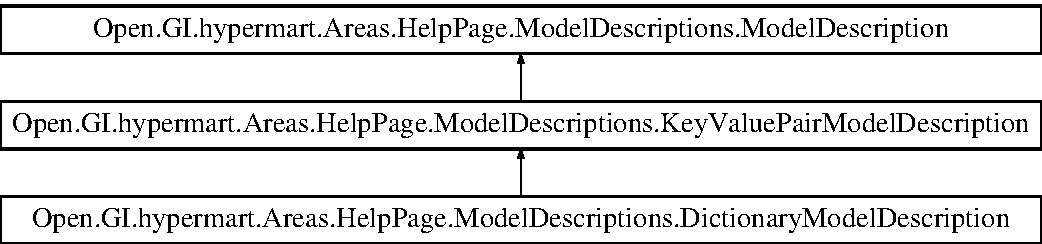
\includegraphics[height=3.000000cm]{class_open_1_1_g_i_1_1hypermart_1_1_areas_1_1_help_page_1_1_model_descriptions_1_1_dictionary_model_description}
\end{center}
\end{figure}
\subsection*{Additional Inherited Members}


\subsection{Detailed Description}


\begin{DoxySeeAlso}{See also}
\hyperlink{class_open_1_1_g_i_1_1hypermart_1_1_areas_1_1_help_page_1_1_model_descriptions_1_1_key_value_pair_model_description}{Open.\+G\+I.\+hypermart.\+Areas.\+Help\+Page.\+Model\+Descriptions.\+Key\+Value\+Pair\+Model\+Description}


\end{DoxySeeAlso}


Definition at line 7 of file Dictionary\+Model\+Description.\+cs.



The documentation for this class was generated from the following file\+:\begin{DoxyCompactItemize}
\item 
C\+:/\+Projects/\+App-\/\+Utility-\/\+Store/\+Open.\+G\+I.\+hypermart/\+Areas/\+Help\+Page/\+Model\+Descriptions/\hyperlink{_dictionary_model_description_8cs}{Dictionary\+Model\+Description.\+cs}\end{DoxyCompactItemize}

\section{Open.\+G\+I.\+hypermart.\+Controllers.\+Download\+Controller Class Reference}
\label{class_open_1_1_g_i_1_1hypermart_1_1_controllers_1_1_download_controller}\index{Open.\+G\+I.\+hypermart.\+Controllers.\+Download\+Controller@{Open.\+G\+I.\+hypermart.\+Controllers.\+Download\+Controller}}


Controller responsible for serving donwload files to the user.  


Inheritance diagram for Open.\+G\+I.\+hypermart.\+Controllers.\+Download\+Controller\+:\begin{figure}[H]
\begin{center}
\leavevmode
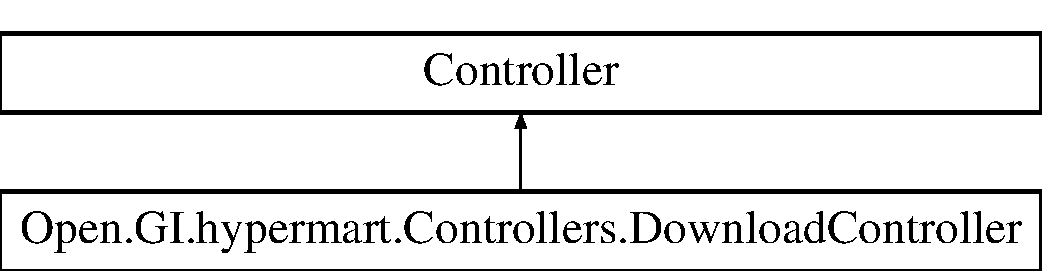
\includegraphics[height=2.000000cm]{class_open_1_1_g_i_1_1hypermart_1_1_controllers_1_1_download_controller}
\end{center}
\end{figure}
\subsection*{Public Member Functions}
\begin{DoxyCompactItemize}
\item 
File\+Result \textbf{ Download} (int id)
\begin{DoxyCompactList}\small\item\em Downloads the specified identifier. \end{DoxyCompactList}\end{DoxyCompactItemize}


\subsection{Detailed Description}
Controller responsible for serving donwload files to the user. 

\begin{DoxySeeAlso}{See also}
System.\+Web.\+Mvc.\+Controller


\end{DoxySeeAlso}


Definition at line 17 of file Download\+Controller.\+cs.



\subsection{Member Function Documentation}
\mbox{\label{class_open_1_1_g_i_1_1hypermart_1_1_controllers_1_1_download_controller_a272d3e80defa78e91555596d44891c47}} 
\index{Open\+::\+G\+I\+::hypermart\+::\+Controllers\+::\+Download\+Controller@{Open\+::\+G\+I\+::hypermart\+::\+Controllers\+::\+Download\+Controller}!Download@{Download}}
\index{Download@{Download}!Open\+::\+G\+I\+::hypermart\+::\+Controllers\+::\+Download\+Controller@{Open\+::\+G\+I\+::hypermart\+::\+Controllers\+::\+Download\+Controller}}
\subsubsection{Download()}
{\footnotesize\ttfamily File\+Result Open.\+G\+I.\+hypermart.\+Controllers.\+Download\+Controller.\+Download (\begin{DoxyParamCaption}\item[{int}]{id }\end{DoxyParamCaption})}



Downloads the specified identifier. 


\begin{DoxyParams}{Parameters}
{\em id} & The identifier.\\
\hline
\end{DoxyParams}
\begin{DoxyReturn}{Returns}

\end{DoxyReturn}

\begin{DoxyExceptions}{Exceptions}
{\em System.\+Web.\+Http\+Exception} & Cannot find file or Cannot find file -\/ can\textquotesingle{}t get remote link. \\
\hline
\end{DoxyExceptions}


Definition at line 30 of file Download\+Controller.\+cs.



The documentation for this class was generated from the following file\+:\begin{DoxyCompactItemize}
\item 
C\+:/\+Projects/\+App-\/\+Utility-\/\+Store/\+Open.\+G\+I.\+hypermart/\+Controllers/\textbf{ Download\+Controller.\+cs}\end{DoxyCompactItemize}

\section{Open.\+G\+I.\+hypermart.\+Areas.\+Help\+Page.\+Model\+Descriptions.\+Enum\+Type\+Model\+Description Class Reference}
\label{class_open_1_1_g_i_1_1hypermart_1_1_areas_1_1_help_page_1_1_model_descriptions_1_1_enum_type_model_description}\index{Open.\+G\+I.\+hypermart.\+Areas.\+Help\+Page.\+Model\+Descriptions.\+Enum\+Type\+Model\+Description@{Open.\+G\+I.\+hypermart.\+Areas.\+Help\+Page.\+Model\+Descriptions.\+Enum\+Type\+Model\+Description}}


 


Inheritance diagram for Open.\+G\+I.\+hypermart.\+Areas.\+Help\+Page.\+Model\+Descriptions.\+Enum\+Type\+Model\+Description\+:\begin{figure}[H]
\begin{center}
\leavevmode
\includegraphics[height=2.000000cm]{class_open_1_1_g_i_1_1hypermart_1_1_areas_1_1_help_page_1_1_model_descriptions_1_1_enum_type_model_description}
\end{center}
\end{figure}
\subsection*{Public Member Functions}
\begin{DoxyCompactItemize}
\item 
\textbf{ Enum\+Type\+Model\+Description} ()
\begin{DoxyCompactList}\small\item\em Initializes a new instance of the \doxyref{Enum\+Type\+Model\+Description}{p.}{class_open_1_1_g_i_1_1hypermart_1_1_areas_1_1_help_page_1_1_model_descriptions_1_1_enum_type_model_description} class. \end{DoxyCompactList}\end{DoxyCompactItemize}
\subsection*{Properties}
\begin{DoxyCompactItemize}
\item 
Collection$<$ \textbf{ Enum\+Value\+Description} $>$ \textbf{ Values}\hspace{0.3cm}{\ttfamily  [get]}
\begin{DoxyCompactList}\small\item\em Gets the values. \end{DoxyCompactList}\end{DoxyCompactItemize}


\subsection{Detailed Description}


\begin{DoxySeeAlso}{See also}
\doxyref{Open.\+G\+I.\+hypermart.\+Areas.\+Help\+Page.\+Model\+Descriptions.\+Model\+Description}{p.}{class_open_1_1_g_i_1_1hypermart_1_1_areas_1_1_help_page_1_1_model_descriptions_1_1_model_description}


\end{DoxySeeAlso}


Definition at line 10 of file Enum\+Type\+Model\+Description.\+cs.



\subsection{Constructor \& Destructor Documentation}
\mbox{\label{class_open_1_1_g_i_1_1hypermart_1_1_areas_1_1_help_page_1_1_model_descriptions_1_1_enum_type_model_description_a77a337dadd9fdcee12869c7385bf51dc}} 
\index{Open\+::\+G\+I\+::hypermart\+::\+Areas\+::\+Help\+Page\+::\+Model\+Descriptions\+::\+Enum\+Type\+Model\+Description@{Open\+::\+G\+I\+::hypermart\+::\+Areas\+::\+Help\+Page\+::\+Model\+Descriptions\+::\+Enum\+Type\+Model\+Description}!Enum\+Type\+Model\+Description@{Enum\+Type\+Model\+Description}}
\index{Enum\+Type\+Model\+Description@{Enum\+Type\+Model\+Description}!Open\+::\+G\+I\+::hypermart\+::\+Areas\+::\+Help\+Page\+::\+Model\+Descriptions\+::\+Enum\+Type\+Model\+Description@{Open\+::\+G\+I\+::hypermart\+::\+Areas\+::\+Help\+Page\+::\+Model\+Descriptions\+::\+Enum\+Type\+Model\+Description}}
\subsubsection{Enum\+Type\+Model\+Description()}
{\footnotesize\ttfamily Open.\+G\+I.\+hypermart.\+Areas.\+Help\+Page.\+Model\+Descriptions.\+Enum\+Type\+Model\+Description.\+Enum\+Type\+Model\+Description (\begin{DoxyParamCaption}{ }\end{DoxyParamCaption})}



Initializes a new instance of the \doxyref{Enum\+Type\+Model\+Description}{p.}{class_open_1_1_g_i_1_1hypermart_1_1_areas_1_1_help_page_1_1_model_descriptions_1_1_enum_type_model_description} class. 



Definition at line 15 of file Enum\+Type\+Model\+Description.\+cs.



\subsection{Property Documentation}
\mbox{\label{class_open_1_1_g_i_1_1hypermart_1_1_areas_1_1_help_page_1_1_model_descriptions_1_1_enum_type_model_description_a7b42c1652865a638dd214ba6a1642819}} 
\index{Open\+::\+G\+I\+::hypermart\+::\+Areas\+::\+Help\+Page\+::\+Model\+Descriptions\+::\+Enum\+Type\+Model\+Description@{Open\+::\+G\+I\+::hypermart\+::\+Areas\+::\+Help\+Page\+::\+Model\+Descriptions\+::\+Enum\+Type\+Model\+Description}!Values@{Values}}
\index{Values@{Values}!Open\+::\+G\+I\+::hypermart\+::\+Areas\+::\+Help\+Page\+::\+Model\+Descriptions\+::\+Enum\+Type\+Model\+Description@{Open\+::\+G\+I\+::hypermart\+::\+Areas\+::\+Help\+Page\+::\+Model\+Descriptions\+::\+Enum\+Type\+Model\+Description}}
\subsubsection{Values}
{\footnotesize\ttfamily Collection$<$\textbf{ Enum\+Value\+Description}$>$ Open.\+G\+I.\+hypermart.\+Areas.\+Help\+Page.\+Model\+Descriptions.\+Enum\+Type\+Model\+Description.\+Values\hspace{0.3cm}{\ttfamily [get]}}



Gets the values. 

The values. 

Definition at line 26 of file Enum\+Type\+Model\+Description.\+cs.



The documentation for this class was generated from the following file\+:\begin{DoxyCompactItemize}
\item 
C\+:/\+Projects/\+App-\/\+Utility-\/\+Store/\+Open.\+G\+I.\+hypermart/\+Areas/\+Help\+Page/\+Model\+Descriptions/\textbf{ Enum\+Type\+Model\+Description.\+cs}\end{DoxyCompactItemize}

\section{Open.\+G\+I.\+hypermart.\+Areas.\+Help\+Page.\+Model\+Descriptions.\+Enum\+Value\+Description Class Reference}
\label{class_open_1_1_g_i_1_1hypermart_1_1_areas_1_1_help_page_1_1_model_descriptions_1_1_enum_value_description}\index{Open.\+G\+I.\+hypermart.\+Areas.\+Help\+Page.\+Model\+Descriptions.\+Enum\+Value\+Description@{Open.\+G\+I.\+hypermart.\+Areas.\+Help\+Page.\+Model\+Descriptions.\+Enum\+Value\+Description}}


 


\subsection*{Properties}
\begin{DoxyCompactItemize}
\item 
string \textbf{ Documentation}\hspace{0.3cm}{\ttfamily  [get, set]}
\begin{DoxyCompactList}\small\item\em Gets or sets the documentation. \end{DoxyCompactList}\item 
string \textbf{ Name}\hspace{0.3cm}{\ttfamily  [get, set]}
\begin{DoxyCompactList}\small\item\em Gets or sets the name. \end{DoxyCompactList}\item 
string \textbf{ Value}\hspace{0.3cm}{\ttfamily  [get, set]}
\begin{DoxyCompactList}\small\item\em Gets or sets the value. \end{DoxyCompactList}\end{DoxyCompactItemize}


\subsection{Detailed Description}




Definition at line 6 of file Enum\+Value\+Description.\+cs.



\subsection{Property Documentation}
\mbox{\label{class_open_1_1_g_i_1_1hypermart_1_1_areas_1_1_help_page_1_1_model_descriptions_1_1_enum_value_description_a8e1e8adc9b367cdc6034e648067585c9}} 
\index{Open\+::\+G\+I\+::hypermart\+::\+Areas\+::\+Help\+Page\+::\+Model\+Descriptions\+::\+Enum\+Value\+Description@{Open\+::\+G\+I\+::hypermart\+::\+Areas\+::\+Help\+Page\+::\+Model\+Descriptions\+::\+Enum\+Value\+Description}!Documentation@{Documentation}}
\index{Documentation@{Documentation}!Open\+::\+G\+I\+::hypermart\+::\+Areas\+::\+Help\+Page\+::\+Model\+Descriptions\+::\+Enum\+Value\+Description@{Open\+::\+G\+I\+::hypermart\+::\+Areas\+::\+Help\+Page\+::\+Model\+Descriptions\+::\+Enum\+Value\+Description}}
\subsubsection{Documentation}
{\footnotesize\ttfamily string Open.\+G\+I.\+hypermart.\+Areas.\+Help\+Page.\+Model\+Descriptions.\+Enum\+Value\+Description.\+Documentation\hspace{0.3cm}{\ttfamily [get]}, {\ttfamily [set]}}



Gets or sets the documentation. 

The documentation. 

Definition at line 14 of file Enum\+Value\+Description.\+cs.

\mbox{\label{class_open_1_1_g_i_1_1hypermart_1_1_areas_1_1_help_page_1_1_model_descriptions_1_1_enum_value_description_a9a7f37f9e6c2a01c41a557b7a8e65d4e}} 
\index{Open\+::\+G\+I\+::hypermart\+::\+Areas\+::\+Help\+Page\+::\+Model\+Descriptions\+::\+Enum\+Value\+Description@{Open\+::\+G\+I\+::hypermart\+::\+Areas\+::\+Help\+Page\+::\+Model\+Descriptions\+::\+Enum\+Value\+Description}!Name@{Name}}
\index{Name@{Name}!Open\+::\+G\+I\+::hypermart\+::\+Areas\+::\+Help\+Page\+::\+Model\+Descriptions\+::\+Enum\+Value\+Description@{Open\+::\+G\+I\+::hypermart\+::\+Areas\+::\+Help\+Page\+::\+Model\+Descriptions\+::\+Enum\+Value\+Description}}
\subsubsection{Name}
{\footnotesize\ttfamily string Open.\+G\+I.\+hypermart.\+Areas.\+Help\+Page.\+Model\+Descriptions.\+Enum\+Value\+Description.\+Name\hspace{0.3cm}{\ttfamily [get]}, {\ttfamily [set]}}



Gets or sets the name. 

The name. 

Definition at line 22 of file Enum\+Value\+Description.\+cs.

\mbox{\label{class_open_1_1_g_i_1_1hypermart_1_1_areas_1_1_help_page_1_1_model_descriptions_1_1_enum_value_description_ab94229a6c9c5afad58abc04d705169f8}} 
\index{Open\+::\+G\+I\+::hypermart\+::\+Areas\+::\+Help\+Page\+::\+Model\+Descriptions\+::\+Enum\+Value\+Description@{Open\+::\+G\+I\+::hypermart\+::\+Areas\+::\+Help\+Page\+::\+Model\+Descriptions\+::\+Enum\+Value\+Description}!Value@{Value}}
\index{Value@{Value}!Open\+::\+G\+I\+::hypermart\+::\+Areas\+::\+Help\+Page\+::\+Model\+Descriptions\+::\+Enum\+Value\+Description@{Open\+::\+G\+I\+::hypermart\+::\+Areas\+::\+Help\+Page\+::\+Model\+Descriptions\+::\+Enum\+Value\+Description}}
\subsubsection{Value}
{\footnotesize\ttfamily string Open.\+G\+I.\+hypermart.\+Areas.\+Help\+Page.\+Model\+Descriptions.\+Enum\+Value\+Description.\+Value\hspace{0.3cm}{\ttfamily [get]}, {\ttfamily [set]}}



Gets or sets the value. 

The value. 

Definition at line 30 of file Enum\+Value\+Description.\+cs.



The documentation for this class was generated from the following file\+:\begin{DoxyCompactItemize}
\item 
C\+:/\+Projects/\+App-\/\+Utility-\/\+Store/\+Open.\+G\+I.\+hypermart/\+Areas/\+Help\+Page/\+Model\+Descriptions/\textbf{ Enum\+Value\+Description.\+cs}\end{DoxyCompactItemize}

\section{Open.\+G\+I.\+hypermart.\+Models.\+File Class Reference}
\label{class_open_1_1_g_i_1_1hypermart_1_1_models_1_1_file}\index{Open.\+G\+I.\+hypermart.\+Models.\+File@{Open.\+G\+I.\+hypermart.\+Models.\+File}}


Model Class representing a \doxyref{File}{p.}{class_open_1_1_g_i_1_1hypermart_1_1_models_1_1_file}.  


\subsection*{Public Member Functions}
\begin{DoxyCompactItemize}
\item 
\textbf{ File} ()
\begin{DoxyCompactList}\small\item\em Initializes a new instance of the \doxyref{File}{p.}{class_open_1_1_g_i_1_1hypermart_1_1_models_1_1_file} class. \end{DoxyCompactList}\item 
\textbf{ File} ()
\end{DoxyCompactItemize}
\subsection*{Properties}
\begin{DoxyCompactItemize}
\item 
int \textbf{ ID}\hspace{0.3cm}{\ttfamily  [get, set]}
\begin{DoxyCompactList}\small\item\em Gets or sets the identifier. \end{DoxyCompactList}\item 
\textbf{ storage\+Type} \textbf{ Storage\+Type}\hspace{0.3cm}{\ttfamily  [get, set]}
\begin{DoxyCompactList}\small\item\em Gets or sets the type of the storage. \end{DoxyCompactList}\item 
string \textbf{ File\+Name}\hspace{0.3cm}{\ttfamily  [get, set]}
\begin{DoxyCompactList}\small\item\em Gets or sets the name of the file. \end{DoxyCompactList}\item 
byte [$\,$] \textbf{ B\+L\+OB}\hspace{0.3cm}{\ttfamily  [get, set]}
\begin{DoxyCompactList}\small\item\em Gets or sets the B\+L\+OB. \end{DoxyCompactList}\item 
string \textbf{ Link}\hspace{0.3cm}{\ttfamily  [get, set]}
\begin{DoxyCompactList}\small\item\em Gets or sets the link. \end{DoxyCompactList}\item 
string \textbf{ Version}\hspace{0.3cm}{\ttfamily  [get, set]}
\begin{DoxyCompactList}\small\item\em Gets or sets the version. \end{DoxyCompactList}\item 
int \textbf{ Product\+ID}\hspace{0.3cm}{\ttfamily  [get, set]}
\begin{DoxyCompactList}\small\item\em Gets or sets the product identifier. \end{DoxyCompactList}\item 
\textbf{ Product} \textbf{ Product}\hspace{0.3cm}{\ttfamily  [get, set]}
\begin{DoxyCompactList}\small\item\em Gets or sets the product. \end{DoxyCompactList}\item 
virtual I\+Collection$<$ \textbf{ Platform} $>$ \textbf{ Platforms}\hspace{0.3cm}{\ttfamily  [get, set]}
\begin{DoxyCompactList}\small\item\em Gets or sets the platforms. \end{DoxyCompactList}\item 
int \textbf{ Storage\+Type}\hspace{0.3cm}{\ttfamily  [get, set]}
\item 
Nullable$<$ int $>$ \textbf{ Product\+ID}\hspace{0.3cm}{\ttfamily  [get, set]}
\item 
virtual \textbf{ Product} \textbf{ Product}\hspace{0.3cm}{\ttfamily  [get, set]}
\item 
virtual I\+Collection$<$ \textbf{ File\+Platform} $>$ \textbf{ File\+Platforms}\hspace{0.3cm}{\ttfamily  [get, set]}
\end{DoxyCompactItemize}


\subsection{Detailed Description}
Model Class representing a \doxyref{File}{p.}{class_open_1_1_g_i_1_1hypermart_1_1_models_1_1_file}. 



Definition at line 12 of file File.\+cs.



\subsection{Constructor \& Destructor Documentation}
\mbox{\label{class_open_1_1_g_i_1_1hypermart_1_1_models_1_1_file_a6834fcf6e0ea0428dc2decfaa974f8d2}} 
\index{Open\+::\+G\+I\+::hypermart\+::\+Models\+::\+File@{Open\+::\+G\+I\+::hypermart\+::\+Models\+::\+File}!File@{File}}
\index{File@{File}!Open\+::\+G\+I\+::hypermart\+::\+Models\+::\+File@{Open\+::\+G\+I\+::hypermart\+::\+Models\+::\+File}}
\subsubsection{File()\hspace{0.1cm}{\footnotesize\ttfamily [1/2]}}
{\footnotesize\ttfamily Open.\+G\+I.\+hypermart.\+Models.\+File.\+File (\begin{DoxyParamCaption}{ }\end{DoxyParamCaption})}



Initializes a new instance of the \doxyref{File}{p.}{class_open_1_1_g_i_1_1hypermart_1_1_models_1_1_file} class. 



Definition at line 18 of file File.\+cs.

\mbox{\label{class_open_1_1_g_i_1_1hypermart_1_1_models_1_1_file_a6834fcf6e0ea0428dc2decfaa974f8d2}} 
\index{Open\+::\+G\+I\+::hypermart\+::\+Models\+::\+File@{Open\+::\+G\+I\+::hypermart\+::\+Models\+::\+File}!File@{File}}
\index{File@{File}!Open\+::\+G\+I\+::hypermart\+::\+Models\+::\+File@{Open\+::\+G\+I\+::hypermart\+::\+Models\+::\+File}}
\subsubsection{File()\hspace{0.1cm}{\footnotesize\ttfamily [2/2]}}
{\footnotesize\ttfamily Open.\+G\+I.\+hypermart.\+Models.\+File.\+File (\begin{DoxyParamCaption}{ }\end{DoxyParamCaption})}



Definition at line 18 of file File.\+cs.



\subsection{Property Documentation}
\mbox{\label{class_open_1_1_g_i_1_1hypermart_1_1_models_1_1_file_acfdfc6e64338fc14a71994e5d7aa5111}} 
\index{Open\+::\+G\+I\+::hypermart\+::\+Models\+::\+File@{Open\+::\+G\+I\+::hypermart\+::\+Models\+::\+File}!B\+L\+OB@{B\+L\+OB}}
\index{B\+L\+OB@{B\+L\+OB}!Open\+::\+G\+I\+::hypermart\+::\+Models\+::\+File@{Open\+::\+G\+I\+::hypermart\+::\+Models\+::\+File}}
\subsubsection{B\+L\+OB}
{\footnotesize\ttfamily byte [$\,$] Open.\+G\+I.\+hypermart.\+Models.\+File.\+B\+L\+OB\hspace{0.3cm}{\ttfamily [get]}, {\ttfamily [set]}}



Gets or sets the B\+L\+OB. 

The B\+L\+OB. 

Definition at line 53 of file File.\+cs.

\mbox{\label{class_open_1_1_g_i_1_1hypermart_1_1_models_1_1_file_a5675dd150dd5ca0de9bc6755fe6c45ad}} 
\index{Open\+::\+G\+I\+::hypermart\+::\+Models\+::\+File@{Open\+::\+G\+I\+::hypermart\+::\+Models\+::\+File}!File\+Name@{File\+Name}}
\index{File\+Name@{File\+Name}!Open\+::\+G\+I\+::hypermart\+::\+Models\+::\+File@{Open\+::\+G\+I\+::hypermart\+::\+Models\+::\+File}}
\subsubsection{File\+Name}
{\footnotesize\ttfamily string Open.\+G\+I.\+hypermart.\+Models.\+File.\+File\+Name\hspace{0.3cm}{\ttfamily [get]}, {\ttfamily [set]}}



Gets or sets the name of the file. 

The name of the file. 

Definition at line 45 of file File.\+cs.

\mbox{\label{class_open_1_1_g_i_1_1hypermart_1_1_models_1_1_file_ac075b378d09c288deda822c0ea6b854c}} 
\index{Open\+::\+G\+I\+::hypermart\+::\+Models\+::\+File@{Open\+::\+G\+I\+::hypermart\+::\+Models\+::\+File}!File\+Platforms@{File\+Platforms}}
\index{File\+Platforms@{File\+Platforms}!Open\+::\+G\+I\+::hypermart\+::\+Models\+::\+File@{Open\+::\+G\+I\+::hypermart\+::\+Models\+::\+File}}
\subsubsection{File\+Platforms}
{\footnotesize\ttfamily virtual I\+Collection$<$\textbf{ File\+Platform}$>$ Open.\+G\+I.\+hypermart.\+Models.\+File.\+File\+Platforms\hspace{0.3cm}{\ttfamily [get]}, {\ttfamily [set]}}



Definition at line 33 of file File.\+cs.

\mbox{\label{class_open_1_1_g_i_1_1hypermart_1_1_models_1_1_file_ade215e549b777e8f30cfa19ec28cff96}} 
\index{Open\+::\+G\+I\+::hypermart\+::\+Models\+::\+File@{Open\+::\+G\+I\+::hypermart\+::\+Models\+::\+File}!ID@{ID}}
\index{ID@{ID}!Open\+::\+G\+I\+::hypermart\+::\+Models\+::\+File@{Open\+::\+G\+I\+::hypermart\+::\+Models\+::\+File}}
\subsubsection{ID}
{\footnotesize\ttfamily int Open.\+G\+I.\+hypermart.\+Models.\+File.\+ID\hspace{0.3cm}{\ttfamily [get]}, {\ttfamily [set]}}



Gets or sets the identifier. 

The identifier. 

Definition at line 29 of file File.\+cs.

\mbox{\label{class_open_1_1_g_i_1_1hypermart_1_1_models_1_1_file_a47b36d33252b1a1f58bee02a94d11dd5}} 
\index{Open\+::\+G\+I\+::hypermart\+::\+Models\+::\+File@{Open\+::\+G\+I\+::hypermart\+::\+Models\+::\+File}!Link@{Link}}
\index{Link@{Link}!Open\+::\+G\+I\+::hypermart\+::\+Models\+::\+File@{Open\+::\+G\+I\+::hypermart\+::\+Models\+::\+File}}
\subsubsection{Link}
{\footnotesize\ttfamily string Open.\+G\+I.\+hypermart.\+Models.\+File.\+Link\hspace{0.3cm}{\ttfamily [get]}, {\ttfamily [set]}}



Gets or sets the link. 

The link. 

Definition at line 61 of file File.\+cs.

\mbox{\label{class_open_1_1_g_i_1_1hypermart_1_1_models_1_1_file_a7cf38ed851b70df6af9b0606c4d744ed}} 
\index{Open\+::\+G\+I\+::hypermart\+::\+Models\+::\+File@{Open\+::\+G\+I\+::hypermart\+::\+Models\+::\+File}!Platforms@{Platforms}}
\index{Platforms@{Platforms}!Open\+::\+G\+I\+::hypermart\+::\+Models\+::\+File@{Open\+::\+G\+I\+::hypermart\+::\+Models\+::\+File}}
\subsubsection{Platforms}
{\footnotesize\ttfamily virtual I\+Collection$<$\textbf{ Platform}$>$ Open.\+G\+I.\+hypermart.\+Models.\+File.\+Platforms\hspace{0.3cm}{\ttfamily [get]}, {\ttfamily [set]}}



Gets or sets the platforms. 

The platforms. 

Definition at line 95 of file File.\+cs.

\mbox{\label{class_open_1_1_g_i_1_1hypermart_1_1_models_1_1_file_a7a2d45936082be844aa8528b298a2d6a}} 
\index{Open\+::\+G\+I\+::hypermart\+::\+Models\+::\+File@{Open\+::\+G\+I\+::hypermart\+::\+Models\+::\+File}!Product@{Product}}
\index{Product@{Product}!Open\+::\+G\+I\+::hypermart\+::\+Models\+::\+File@{Open\+::\+G\+I\+::hypermart\+::\+Models\+::\+File}}
\subsubsection{Product\hspace{0.1cm}{\footnotesize\ttfamily [1/2]}}
{\footnotesize\ttfamily virtual \textbf{ Product} Open.\+G\+I.\+hypermart.\+Models.\+File.\+Product\hspace{0.3cm}{\ttfamily [get]}, {\ttfamily [set]}}



Definition at line 31 of file File.\+cs.

\mbox{\label{class_open_1_1_g_i_1_1hypermart_1_1_models_1_1_file_a4b8d3f1af1802269e9e06285f9bf81b3}} 
\index{Open\+::\+G\+I\+::hypermart\+::\+Models\+::\+File@{Open\+::\+G\+I\+::hypermart\+::\+Models\+::\+File}!Product@{Product}}
\index{Product@{Product}!Open\+::\+G\+I\+::hypermart\+::\+Models\+::\+File@{Open\+::\+G\+I\+::hypermart\+::\+Models\+::\+File}}
\subsubsection{Product\hspace{0.1cm}{\footnotesize\ttfamily [2/2]}}
{\footnotesize\ttfamily \textbf{ Product} Open.\+G\+I.\+hypermart.\+Models.\+File.\+Product\hspace{0.3cm}{\ttfamily [get]}, {\ttfamily [set]}}



Gets or sets the product. 

The product. 

Definition at line 86 of file File.\+cs.

\mbox{\label{class_open_1_1_g_i_1_1hypermart_1_1_models_1_1_file_ad0b974d38df4491ce90d1d5e884a56a8}} 
\index{Open\+::\+G\+I\+::hypermart\+::\+Models\+::\+File@{Open\+::\+G\+I\+::hypermart\+::\+Models\+::\+File}!Product\+ID@{Product\+ID}}
\index{Product\+ID@{Product\+ID}!Open\+::\+G\+I\+::hypermart\+::\+Models\+::\+File@{Open\+::\+G\+I\+::hypermart\+::\+Models\+::\+File}}
\subsubsection{Product\+ID\hspace{0.1cm}{\footnotesize\ttfamily [1/2]}}
{\footnotesize\ttfamily Nullable$<$int$>$ Open.\+G\+I.\+hypermart.\+Models.\+File.\+Product\+ID\hspace{0.3cm}{\ttfamily [get]}, {\ttfamily [set]}}



Definition at line 29 of file File.\+cs.

\mbox{\label{class_open_1_1_g_i_1_1hypermart_1_1_models_1_1_file_a7f0a3da01808662b23635d9b9b6f6848}} 
\index{Open\+::\+G\+I\+::hypermart\+::\+Models\+::\+File@{Open\+::\+G\+I\+::hypermart\+::\+Models\+::\+File}!Product\+ID@{Product\+ID}}
\index{Product\+ID@{Product\+ID}!Open\+::\+G\+I\+::hypermart\+::\+Models\+::\+File@{Open\+::\+G\+I\+::hypermart\+::\+Models\+::\+File}}
\subsubsection{Product\+ID\hspace{0.1cm}{\footnotesize\ttfamily [2/2]}}
{\footnotesize\ttfamily int Open.\+G\+I.\+hypermart.\+Models.\+File.\+Product\+ID\hspace{0.3cm}{\ttfamily [get]}, {\ttfamily [set]}}



Gets or sets the product identifier. 

The product identifier. 

Definition at line 78 of file File.\+cs.

\mbox{\label{class_open_1_1_g_i_1_1hypermart_1_1_models_1_1_file_ab4ac8af085696918a7a4e1765639066d}} 
\index{Open\+::\+G\+I\+::hypermart\+::\+Models\+::\+File@{Open\+::\+G\+I\+::hypermart\+::\+Models\+::\+File}!Storage\+Type@{Storage\+Type}}
\index{Storage\+Type@{Storage\+Type}!Open\+::\+G\+I\+::hypermart\+::\+Models\+::\+File@{Open\+::\+G\+I\+::hypermart\+::\+Models\+::\+File}}
\subsubsection{Storage\+Type\hspace{0.1cm}{\footnotesize\ttfamily [1/2]}}
{\footnotesize\ttfamily int Open.\+G\+I.\+hypermart.\+Models.\+File.\+Storage\+Type\hspace{0.3cm}{\ttfamily [get]}, {\ttfamily [set]}}



Definition at line 24 of file File.\+cs.

\mbox{\label{class_open_1_1_g_i_1_1hypermart_1_1_models_1_1_file_a4d6910e1f3277beb5b50309e8139a356}} 
\index{Open\+::\+G\+I\+::hypermart\+::\+Models\+::\+File@{Open\+::\+G\+I\+::hypermart\+::\+Models\+::\+File}!Storage\+Type@{Storage\+Type}}
\index{Storage\+Type@{Storage\+Type}!Open\+::\+G\+I\+::hypermart\+::\+Models\+::\+File@{Open\+::\+G\+I\+::hypermart\+::\+Models\+::\+File}}
\subsubsection{Storage\+Type\hspace{0.1cm}{\footnotesize\ttfamily [2/2]}}
{\footnotesize\ttfamily \textbf{ storage\+Type} Open.\+G\+I.\+hypermart.\+Models.\+File.\+Storage\+Type\hspace{0.3cm}{\ttfamily [get]}, {\ttfamily [set]}}



Gets or sets the type of the storage. 

The type of the storage. 

Definition at line 37 of file File.\+cs.

\mbox{\label{class_open_1_1_g_i_1_1hypermart_1_1_models_1_1_file_a59b1cbe55394fce55d55200ea7e55cae}} 
\index{Open\+::\+G\+I\+::hypermart\+::\+Models\+::\+File@{Open\+::\+G\+I\+::hypermart\+::\+Models\+::\+File}!Version@{Version}}
\index{Version@{Version}!Open\+::\+G\+I\+::hypermart\+::\+Models\+::\+File@{Open\+::\+G\+I\+::hypermart\+::\+Models\+::\+File}}
\subsubsection{Version}
{\footnotesize\ttfamily string Open.\+G\+I.\+hypermart.\+Models.\+File.\+Version\hspace{0.3cm}{\ttfamily [get]}, {\ttfamily [set]}}



Gets or sets the version. 

The version. 

Definition at line 70 of file File.\+cs.



The documentation for this class was generated from the following file\+:\begin{DoxyCompactItemize}
\item 
C\+:/\+Projects/\+App-\/\+Utility-\/\+Store/\+Open.\+G\+I.\+hypermart/\+Models/\textbf{ File.\+cs}\end{DoxyCompactItemize}

\section{Open.\+G\+I.\+hypermart.\+Data\+Transformation\+Objects.\+File\+D\+TO Class Reference}
\label{class_open_1_1_g_i_1_1hypermart_1_1_data_transformation_objects_1_1_file_d_t_o}\index{Open.\+G\+I.\+hypermart.\+Data\+Transformation\+Objects.\+File\+D\+TO@{Open.\+G\+I.\+hypermart.\+Data\+Transformation\+Objects.\+File\+D\+TO}}


 


\subsection*{Public Member Functions}
\begin{DoxyCompactItemize}
\item 
\textbf{ File\+D\+TO} ()
\begin{DoxyCompactList}\small\item\em Initializes a new instance of the \doxyref{File\+D\+TO}{p.}{class_open_1_1_g_i_1_1hypermart_1_1_data_transformation_objects_1_1_file_d_t_o} class. \end{DoxyCompactList}\item 
\textbf{ File\+D\+TO} (\textbf{ File} \textbf{ File})
\begin{DoxyCompactList}\small\item\em Initializes a new instance of the \doxyref{File\+D\+TO}{p.}{class_open_1_1_g_i_1_1hypermart_1_1_data_transformation_objects_1_1_file_d_t_o} class. \end{DoxyCompactList}\end{DoxyCompactItemize}
\subsection*{Properties}
\begin{DoxyCompactItemize}
\item 
int \textbf{ ID}\hspace{0.3cm}{\ttfamily  [get, set]}
\begin{DoxyCompactList}\small\item\em Gets or sets the identifier. \end{DoxyCompactList}\item 
\textbf{ storage\+Type} \textbf{ Storage\+Type}\hspace{0.3cm}{\ttfamily  [get, set]}
\begin{DoxyCompactList}\small\item\em Gets or sets the type of the storage. \end{DoxyCompactList}\item 
string \textbf{ File\+Name}\hspace{0.3cm}{\ttfamily  [get, set]}
\begin{DoxyCompactList}\small\item\em Gets or sets the name of the file. \end{DoxyCompactList}\item 
byte [$\,$] \textbf{ B\+L\+OB}\hspace{0.3cm}{\ttfamily  [get, set]}
\begin{DoxyCompactList}\small\item\em Gets or sets the B\+L\+OB. \end{DoxyCompactList}\item 
string \textbf{ Link}\hspace{0.3cm}{\ttfamily  [get, set]}
\begin{DoxyCompactList}\small\item\em Gets or sets the link. \end{DoxyCompactList}\item 
string \textbf{ Version}\hspace{0.3cm}{\ttfamily  [get, set]}
\begin{DoxyCompactList}\small\item\em Gets or sets the version. \end{DoxyCompactList}\item 
int \textbf{ Product\+ID}\hspace{0.3cm}{\ttfamily  [get, set]}
\begin{DoxyCompactList}\small\item\em Gets or sets the product identifier. \end{DoxyCompactList}\item 
virtual \textbf{ Product} \textbf{ Product}\hspace{0.3cm}{\ttfamily  [get, set]}
\begin{DoxyCompactList}\small\item\em Gets or sets the product. \end{DoxyCompactList}\item 
virtual I\+Collection$<$ \textbf{ Platform} $>$ \textbf{ Platforms}\hspace{0.3cm}{\ttfamily  [get, set]}
\begin{DoxyCompactList}\small\item\em Gets or sets the platforms. \end{DoxyCompactList}\end{DoxyCompactItemize}


\subsection{Detailed Description}




Definition at line 14 of file File\+D\+T\+O.\+cs.



\subsection{Constructor \& Destructor Documentation}
\mbox{\label{class_open_1_1_g_i_1_1hypermart_1_1_data_transformation_objects_1_1_file_d_t_o_ae0da87388dbf076d2aa151cce63c81a8}} 
\index{Open\+::\+G\+I\+::hypermart\+::\+Data\+Transformation\+Objects\+::\+File\+D\+TO@{Open\+::\+G\+I\+::hypermart\+::\+Data\+Transformation\+Objects\+::\+File\+D\+TO}!File\+D\+TO@{File\+D\+TO}}
\index{File\+D\+TO@{File\+D\+TO}!Open\+::\+G\+I\+::hypermart\+::\+Data\+Transformation\+Objects\+::\+File\+D\+TO@{Open\+::\+G\+I\+::hypermart\+::\+Data\+Transformation\+Objects\+::\+File\+D\+TO}}
\subsubsection{File\+D\+T\+O()\hspace{0.1cm}{\footnotesize\ttfamily [1/2]}}
{\footnotesize\ttfamily Open.\+G\+I.\+hypermart.\+Data\+Transformation\+Objects.\+File\+D\+T\+O.\+File\+D\+TO (\begin{DoxyParamCaption}{ }\end{DoxyParamCaption})}



Initializes a new instance of the \doxyref{File\+D\+TO}{p.}{class_open_1_1_g_i_1_1hypermart_1_1_data_transformation_objects_1_1_file_d_t_o} class. 



Definition at line 19 of file File\+D\+T\+O.\+cs.

\mbox{\label{class_open_1_1_g_i_1_1hypermart_1_1_data_transformation_objects_1_1_file_d_t_o_add1a3ae47dca46ed24d3d8dda310a3a2}} 
\index{Open\+::\+G\+I\+::hypermart\+::\+Data\+Transformation\+Objects\+::\+File\+D\+TO@{Open\+::\+G\+I\+::hypermart\+::\+Data\+Transformation\+Objects\+::\+File\+D\+TO}!File\+D\+TO@{File\+D\+TO}}
\index{File\+D\+TO@{File\+D\+TO}!Open\+::\+G\+I\+::hypermart\+::\+Data\+Transformation\+Objects\+::\+File\+D\+TO@{Open\+::\+G\+I\+::hypermart\+::\+Data\+Transformation\+Objects\+::\+File\+D\+TO}}
\subsubsection{File\+D\+T\+O()\hspace{0.1cm}{\footnotesize\ttfamily [2/2]}}
{\footnotesize\ttfamily Open.\+G\+I.\+hypermart.\+Data\+Transformation\+Objects.\+File\+D\+T\+O.\+File\+D\+TO (\begin{DoxyParamCaption}\item[{\textbf{ File}}]{File }\end{DoxyParamCaption})}



Initializes a new instance of the \doxyref{File\+D\+TO}{p.}{class_open_1_1_g_i_1_1hypermart_1_1_data_transformation_objects_1_1_file_d_t_o} class. 


\begin{DoxyParams}{Parameters}
{\em File} & The file.\\
\hline
\end{DoxyParams}


Definition at line 28 of file File\+D\+T\+O.\+cs.



\subsection{Property Documentation}
\mbox{\label{class_open_1_1_g_i_1_1hypermart_1_1_data_transformation_objects_1_1_file_d_t_o_af2ebb686a878cb8342e76648d048f19a}} 
\index{Open\+::\+G\+I\+::hypermart\+::\+Data\+Transformation\+Objects\+::\+File\+D\+TO@{Open\+::\+G\+I\+::hypermart\+::\+Data\+Transformation\+Objects\+::\+File\+D\+TO}!B\+L\+OB@{B\+L\+OB}}
\index{B\+L\+OB@{B\+L\+OB}!Open\+::\+G\+I\+::hypermart\+::\+Data\+Transformation\+Objects\+::\+File\+D\+TO@{Open\+::\+G\+I\+::hypermart\+::\+Data\+Transformation\+Objects\+::\+File\+D\+TO}}
\subsubsection{B\+L\+OB}
{\footnotesize\ttfamily byte [$\,$] Open.\+G\+I.\+hypermart.\+Data\+Transformation\+Objects.\+File\+D\+T\+O.\+B\+L\+OB\hspace{0.3cm}{\ttfamily [get]}, {\ttfamily [set]}}



Gets or sets the B\+L\+OB. 

The B\+L\+OB. 

Definition at line 71 of file File\+D\+T\+O.\+cs.

\mbox{\label{class_open_1_1_g_i_1_1hypermart_1_1_data_transformation_objects_1_1_file_d_t_o_a55fb34aacab9513037108ff3f1d287a8}} 
\index{Open\+::\+G\+I\+::hypermart\+::\+Data\+Transformation\+Objects\+::\+File\+D\+TO@{Open\+::\+G\+I\+::hypermart\+::\+Data\+Transformation\+Objects\+::\+File\+D\+TO}!File\+Name@{File\+Name}}
\index{File\+Name@{File\+Name}!Open\+::\+G\+I\+::hypermart\+::\+Data\+Transformation\+Objects\+::\+File\+D\+TO@{Open\+::\+G\+I\+::hypermart\+::\+Data\+Transformation\+Objects\+::\+File\+D\+TO}}
\subsubsection{File\+Name}
{\footnotesize\ttfamily string Open.\+G\+I.\+hypermart.\+Data\+Transformation\+Objects.\+File\+D\+T\+O.\+File\+Name\hspace{0.3cm}{\ttfamily [get]}, {\ttfamily [set]}}



Gets or sets the name of the file. 

The name of the file. 

Definition at line 63 of file File\+D\+T\+O.\+cs.

\mbox{\label{class_open_1_1_g_i_1_1hypermart_1_1_data_transformation_objects_1_1_file_d_t_o_ab187e7f070650067d055de8f707e1eed}} 
\index{Open\+::\+G\+I\+::hypermart\+::\+Data\+Transformation\+Objects\+::\+File\+D\+TO@{Open\+::\+G\+I\+::hypermart\+::\+Data\+Transformation\+Objects\+::\+File\+D\+TO}!ID@{ID}}
\index{ID@{ID}!Open\+::\+G\+I\+::hypermart\+::\+Data\+Transformation\+Objects\+::\+File\+D\+TO@{Open\+::\+G\+I\+::hypermart\+::\+Data\+Transformation\+Objects\+::\+File\+D\+TO}}
\subsubsection{ID}
{\footnotesize\ttfamily int Open.\+G\+I.\+hypermart.\+Data\+Transformation\+Objects.\+File\+D\+T\+O.\+ID\hspace{0.3cm}{\ttfamily [get]}, {\ttfamily [set]}}



Gets or sets the identifier. 

The identifier. 

Definition at line 47 of file File\+D\+T\+O.\+cs.

\mbox{\label{class_open_1_1_g_i_1_1hypermart_1_1_data_transformation_objects_1_1_file_d_t_o_af58091e5ba2e9fde7db92f08dc4d3a41}} 
\index{Open\+::\+G\+I\+::hypermart\+::\+Data\+Transformation\+Objects\+::\+File\+D\+TO@{Open\+::\+G\+I\+::hypermart\+::\+Data\+Transformation\+Objects\+::\+File\+D\+TO}!Link@{Link}}
\index{Link@{Link}!Open\+::\+G\+I\+::hypermart\+::\+Data\+Transformation\+Objects\+::\+File\+D\+TO@{Open\+::\+G\+I\+::hypermart\+::\+Data\+Transformation\+Objects\+::\+File\+D\+TO}}
\subsubsection{Link}
{\footnotesize\ttfamily string Open.\+G\+I.\+hypermart.\+Data\+Transformation\+Objects.\+File\+D\+T\+O.\+Link\hspace{0.3cm}{\ttfamily [get]}, {\ttfamily [set]}}



Gets or sets the link. 

The link. 

Definition at line 79 of file File\+D\+T\+O.\+cs.

\mbox{\label{class_open_1_1_g_i_1_1hypermart_1_1_data_transformation_objects_1_1_file_d_t_o_a784824c36cab74d3bc03a8ae55d9a62a}} 
\index{Open\+::\+G\+I\+::hypermart\+::\+Data\+Transformation\+Objects\+::\+File\+D\+TO@{Open\+::\+G\+I\+::hypermart\+::\+Data\+Transformation\+Objects\+::\+File\+D\+TO}!Platforms@{Platforms}}
\index{Platforms@{Platforms}!Open\+::\+G\+I\+::hypermart\+::\+Data\+Transformation\+Objects\+::\+File\+D\+TO@{Open\+::\+G\+I\+::hypermart\+::\+Data\+Transformation\+Objects\+::\+File\+D\+TO}}
\subsubsection{Platforms}
{\footnotesize\ttfamily virtual I\+Collection$<$\textbf{ Platform}$>$ Open.\+G\+I.\+hypermart.\+Data\+Transformation\+Objects.\+File\+D\+T\+O.\+Platforms\hspace{0.3cm}{\ttfamily [get]}, {\ttfamily [set]}}



Gets or sets the platforms. 

The platforms. 

Definition at line 112 of file File\+D\+T\+O.\+cs.

\mbox{\label{class_open_1_1_g_i_1_1hypermart_1_1_data_transformation_objects_1_1_file_d_t_o_aa587dd986d4c6d62d8bf5520d3a48e79}} 
\index{Open\+::\+G\+I\+::hypermart\+::\+Data\+Transformation\+Objects\+::\+File\+D\+TO@{Open\+::\+G\+I\+::hypermart\+::\+Data\+Transformation\+Objects\+::\+File\+D\+TO}!Product@{Product}}
\index{Product@{Product}!Open\+::\+G\+I\+::hypermart\+::\+Data\+Transformation\+Objects\+::\+File\+D\+TO@{Open\+::\+G\+I\+::hypermart\+::\+Data\+Transformation\+Objects\+::\+File\+D\+TO}}
\subsubsection{Product}
{\footnotesize\ttfamily virtual \textbf{ Product} Open.\+G\+I.\+hypermart.\+Data\+Transformation\+Objects.\+File\+D\+T\+O.\+Product\hspace{0.3cm}{\ttfamily [get]}, {\ttfamily [set]}}



Gets or sets the product. 

The product. 

Definition at line 104 of file File\+D\+T\+O.\+cs.

\mbox{\label{class_open_1_1_g_i_1_1hypermart_1_1_data_transformation_objects_1_1_file_d_t_o_abd8d9083fbb95dac1e2781f2a8d4f8e9}} 
\index{Open\+::\+G\+I\+::hypermart\+::\+Data\+Transformation\+Objects\+::\+File\+D\+TO@{Open\+::\+G\+I\+::hypermart\+::\+Data\+Transformation\+Objects\+::\+File\+D\+TO}!Product\+ID@{Product\+ID}}
\index{Product\+ID@{Product\+ID}!Open\+::\+G\+I\+::hypermart\+::\+Data\+Transformation\+Objects\+::\+File\+D\+TO@{Open\+::\+G\+I\+::hypermart\+::\+Data\+Transformation\+Objects\+::\+File\+D\+TO}}
\subsubsection{Product\+ID}
{\footnotesize\ttfamily int Open.\+G\+I.\+hypermart.\+Data\+Transformation\+Objects.\+File\+D\+T\+O.\+Product\+ID\hspace{0.3cm}{\ttfamily [get]}, {\ttfamily [set]}}



Gets or sets the product identifier. 

The product identifier. 

Definition at line 96 of file File\+D\+T\+O.\+cs.

\mbox{\label{class_open_1_1_g_i_1_1hypermart_1_1_data_transformation_objects_1_1_file_d_t_o_a4563713ee116eb1163eaac1f242b395f}} 
\index{Open\+::\+G\+I\+::hypermart\+::\+Data\+Transformation\+Objects\+::\+File\+D\+TO@{Open\+::\+G\+I\+::hypermart\+::\+Data\+Transformation\+Objects\+::\+File\+D\+TO}!Storage\+Type@{Storage\+Type}}
\index{Storage\+Type@{Storage\+Type}!Open\+::\+G\+I\+::hypermart\+::\+Data\+Transformation\+Objects\+::\+File\+D\+TO@{Open\+::\+G\+I\+::hypermart\+::\+Data\+Transformation\+Objects\+::\+File\+D\+TO}}
\subsubsection{Storage\+Type}
{\footnotesize\ttfamily \textbf{ storage\+Type} Open.\+G\+I.\+hypermart.\+Data\+Transformation\+Objects.\+File\+D\+T\+O.\+Storage\+Type\hspace{0.3cm}{\ttfamily [get]}, {\ttfamily [set]}}



Gets or sets the type of the storage. 

The type of the storage. 

Definition at line 55 of file File\+D\+T\+O.\+cs.

\mbox{\label{class_open_1_1_g_i_1_1hypermart_1_1_data_transformation_objects_1_1_file_d_t_o_ac55a6e7062078277eed54e42b7c29d73}} 
\index{Open\+::\+G\+I\+::hypermart\+::\+Data\+Transformation\+Objects\+::\+File\+D\+TO@{Open\+::\+G\+I\+::hypermart\+::\+Data\+Transformation\+Objects\+::\+File\+D\+TO}!Version@{Version}}
\index{Version@{Version}!Open\+::\+G\+I\+::hypermart\+::\+Data\+Transformation\+Objects\+::\+File\+D\+TO@{Open\+::\+G\+I\+::hypermart\+::\+Data\+Transformation\+Objects\+::\+File\+D\+TO}}
\subsubsection{Version}
{\footnotesize\ttfamily string Open.\+G\+I.\+hypermart.\+Data\+Transformation\+Objects.\+File\+D\+T\+O.\+Version\hspace{0.3cm}{\ttfamily [get]}, {\ttfamily [set]}}



Gets or sets the version. 

The version. 

Definition at line 88 of file File\+D\+T\+O.\+cs.



The documentation for this class was generated from the following file\+:\begin{DoxyCompactItemize}
\item 
C\+:/\+Projects/\+App-\/\+Utility-\/\+Store/\+Open.\+G\+I.\+hypermart/\+Docs/\+Data\+Transformation\+Objects/\textbf{ File\+D\+T\+O.\+cs}\end{DoxyCompactItemize}

\hypertarget{class_open_1_1_g_i_1_1hypermart_1_1_models_1_1_file_platform}{}\section{Open.\+G\+I.\+hypermart.\+Models.\+File\+Platform Class Reference}
\label{class_open_1_1_g_i_1_1hypermart_1_1_models_1_1_file_platform}\index{Open.\+G\+I.\+hypermart.\+Models.\+File\+Platform@{Open.\+G\+I.\+hypermart.\+Models.\+File\+Platform}}
\subsection*{Properties}
\begin{DoxyCompactItemize}
\item 
int \hyperlink{class_open_1_1_g_i_1_1hypermart_1_1_models_1_1_file_platform_a6a2b6dbace772016d649b3feb7c65e44}{Files\+\_\+\+ID}\hspace{0.3cm}{\ttfamily  \mbox{[}get, set\mbox{]}}
\item 
string \hyperlink{class_open_1_1_g_i_1_1hypermart_1_1_models_1_1_file_platform_afe9e1d6e156cababf5d2123d21556d5f}{Platforms\+\_\+\+ID}\hspace{0.3cm}{\ttfamily  \mbox{[}get, set\mbox{]}}
\item 
virtual \hyperlink{class_open_1_1_g_i_1_1hypermart_1_1_models_1_1_platform}{Platform} \hyperlink{class_open_1_1_g_i_1_1hypermart_1_1_models_1_1_file_platform_aeab28cbe72f89ee18f61510d8ea2b7bc}{Platform}\hspace{0.3cm}{\ttfamily  \mbox{[}get, set\mbox{]}}
\item 
virtual \hyperlink{class_open_1_1_g_i_1_1hypermart_1_1_models_1_1_file}{File} \hyperlink{class_open_1_1_g_i_1_1hypermart_1_1_models_1_1_file_platform_aa9fd91411ba71f8dd77bdba062daecd3}{File}\hspace{0.3cm}{\ttfamily  \mbox{[}get, set\mbox{]}}
\end{DoxyCompactItemize}


\subsection{Property Documentation}
\hypertarget{class_open_1_1_g_i_1_1hypermart_1_1_models_1_1_file_platform_aa9fd91411ba71f8dd77bdba062daecd3}{}\label{class_open_1_1_g_i_1_1hypermart_1_1_models_1_1_file_platform_aa9fd91411ba71f8dd77bdba062daecd3} 
\index{Open\+::\+G\+I\+::hypermart\+::\+Models\+::\+File\+Platform@{Open\+::\+G\+I\+::hypermart\+::\+Models\+::\+File\+Platform}!File@{File}}
\index{File@{File}!Open\+::\+G\+I\+::hypermart\+::\+Models\+::\+File\+Platform@{Open\+::\+G\+I\+::hypermart\+::\+Models\+::\+File\+Platform}}
\subsubsection{\texorpdfstring{File}{File}}
{\footnotesize\ttfamily virtual \hyperlink{class_open_1_1_g_i_1_1hypermart_1_1_models_1_1_file}{File} Open.\+G\+I.\+hypermart.\+Models.\+File\+Platform.\+File\hspace{0.3cm}{\ttfamily [get]}, {\ttfamily [set]}}

\hypertarget{class_open_1_1_g_i_1_1hypermart_1_1_models_1_1_file_platform_a6a2b6dbace772016d649b3feb7c65e44}{}\label{class_open_1_1_g_i_1_1hypermart_1_1_models_1_1_file_platform_a6a2b6dbace772016d649b3feb7c65e44} 
\index{Open\+::\+G\+I\+::hypermart\+::\+Models\+::\+File\+Platform@{Open\+::\+G\+I\+::hypermart\+::\+Models\+::\+File\+Platform}!Files\+\_\+\+ID@{Files\+\_\+\+ID}}
\index{Files\+\_\+\+ID@{Files\+\_\+\+ID}!Open\+::\+G\+I\+::hypermart\+::\+Models\+::\+File\+Platform@{Open\+::\+G\+I\+::hypermart\+::\+Models\+::\+File\+Platform}}
\subsubsection{\texorpdfstring{Files\+\_\+\+ID}{Files\_ID}}
{\footnotesize\ttfamily int Open.\+G\+I.\+hypermart.\+Models.\+File\+Platform.\+Files\+\_\+\+ID\hspace{0.3cm}{\ttfamily [get]}, {\ttfamily [set]}}

\hypertarget{class_open_1_1_g_i_1_1hypermart_1_1_models_1_1_file_platform_aeab28cbe72f89ee18f61510d8ea2b7bc}{}\label{class_open_1_1_g_i_1_1hypermart_1_1_models_1_1_file_platform_aeab28cbe72f89ee18f61510d8ea2b7bc} 
\index{Open\+::\+G\+I\+::hypermart\+::\+Models\+::\+File\+Platform@{Open\+::\+G\+I\+::hypermart\+::\+Models\+::\+File\+Platform}!Platform@{Platform}}
\index{Platform@{Platform}!Open\+::\+G\+I\+::hypermart\+::\+Models\+::\+File\+Platform@{Open\+::\+G\+I\+::hypermart\+::\+Models\+::\+File\+Platform}}
\subsubsection{\texorpdfstring{Platform}{Platform}}
{\footnotesize\ttfamily virtual \hyperlink{class_open_1_1_g_i_1_1hypermart_1_1_models_1_1_platform}{Platform} Open.\+G\+I.\+hypermart.\+Models.\+File\+Platform.\+Platform\hspace{0.3cm}{\ttfamily [get]}, {\ttfamily [set]}}

\hypertarget{class_open_1_1_g_i_1_1hypermart_1_1_models_1_1_file_platform_afe9e1d6e156cababf5d2123d21556d5f}{}\label{class_open_1_1_g_i_1_1hypermart_1_1_models_1_1_file_platform_afe9e1d6e156cababf5d2123d21556d5f} 
\index{Open\+::\+G\+I\+::hypermart\+::\+Models\+::\+File\+Platform@{Open\+::\+G\+I\+::hypermart\+::\+Models\+::\+File\+Platform}!Platforms\+\_\+\+ID@{Platforms\+\_\+\+ID}}
\index{Platforms\+\_\+\+ID@{Platforms\+\_\+\+ID}!Open\+::\+G\+I\+::hypermart\+::\+Models\+::\+File\+Platform@{Open\+::\+G\+I\+::hypermart\+::\+Models\+::\+File\+Platform}}
\subsubsection{\texorpdfstring{Platforms\+\_\+\+ID}{Platforms\_ID}}
{\footnotesize\ttfamily string Open.\+G\+I.\+hypermart.\+Models.\+File\+Platform.\+Platforms\+\_\+\+ID\hspace{0.3cm}{\ttfamily [get]}, {\ttfamily [set]}}



The documentation for this class was generated from the following file\+:\begin{DoxyCompactItemize}
\item 
C\+:/\+Projects/\+App-\/\+Utility-\/\+Store/\+Open.\+G\+I.\+hypermart/\+W\+I\+P/\hyperlink{_file_platform_8cs}{File\+Platform.\+cs}\end{DoxyCompactItemize}

\section{Open.\+G\+I.\+hypermart.\+Helpers.\+File\+Share\+Helper Class Reference}
\label{class_open_1_1_g_i_1_1hypermart_1_1_helpers_1_1_file_share_helper}\index{Open.\+G\+I.\+hypermart.\+Helpers.\+File\+Share\+Helper@{Open.\+G\+I.\+hypermart.\+Helpers.\+File\+Share\+Helper}}


 


\subsection*{Static Public Member Functions}
\begin{DoxyCompactItemize}
\item 
static void \textbf{ Create\+Folder} (String Folder\+Name)
\begin{DoxyCompactList}\small\item\em Create a Folder -\/ used to create a file System for storing products \end{DoxyCompactList}\item 
static void \textbf{ Create\+Share} (string Folder\+Name, string Share\+Name, string Description)
\begin{DoxyCompactList}\small\item\em Creates the share. \end{DoxyCompactList}\item 
static void \textbf{ Delete\+Share} (string Folder\+Name)
\begin{DoxyCompactList}\small\item\em Deletes the share. \end{DoxyCompactList}\end{DoxyCompactItemize}


\subsection{Detailed Description}




Definition at line 56 of file File\+Share\+Helper.\+cs.



\subsection{Member Function Documentation}
\mbox{\label{class_open_1_1_g_i_1_1hypermart_1_1_helpers_1_1_file_share_helper_a8e938d7ae2d931ab892c0ebf964ee4d2}} 
\index{Open\+::\+G\+I\+::hypermart\+::\+Helpers\+::\+File\+Share\+Helper@{Open\+::\+G\+I\+::hypermart\+::\+Helpers\+::\+File\+Share\+Helper}!Create\+Folder@{Create\+Folder}}
\index{Create\+Folder@{Create\+Folder}!Open\+::\+G\+I\+::hypermart\+::\+Helpers\+::\+File\+Share\+Helper@{Open\+::\+G\+I\+::hypermart\+::\+Helpers\+::\+File\+Share\+Helper}}
\subsubsection{Create\+Folder()}
{\footnotesize\ttfamily static void Open.\+G\+I.\+hypermart.\+Helpers.\+File\+Share\+Helper.\+Create\+Folder (\begin{DoxyParamCaption}\item[{String}]{Folder\+Name }\end{DoxyParamCaption})\hspace{0.3cm}{\ttfamily [static]}}



Create a Folder -\/ used to create a file System for storing products 


\begin{DoxyParams}{Parameters}
{\em Folder\+Name} & \\
\hline
\end{DoxyParams}


Definition at line 62 of file File\+Share\+Helper.\+cs.

\mbox{\label{class_open_1_1_g_i_1_1hypermart_1_1_helpers_1_1_file_share_helper_af08f7c0abe722a41623b0ae56f78a927}} 
\index{Open\+::\+G\+I\+::hypermart\+::\+Helpers\+::\+File\+Share\+Helper@{Open\+::\+G\+I\+::hypermart\+::\+Helpers\+::\+File\+Share\+Helper}!Create\+Share@{Create\+Share}}
\index{Create\+Share@{Create\+Share}!Open\+::\+G\+I\+::hypermart\+::\+Helpers\+::\+File\+Share\+Helper@{Open\+::\+G\+I\+::hypermart\+::\+Helpers\+::\+File\+Share\+Helper}}
\subsubsection{Create\+Share()}
{\footnotesize\ttfamily static void Open.\+G\+I.\+hypermart.\+Helpers.\+File\+Share\+Helper.\+Create\+Share (\begin{DoxyParamCaption}\item[{string}]{Folder\+Name,  }\item[{string}]{Share\+Name,  }\item[{string}]{Description }\end{DoxyParamCaption})\hspace{0.3cm}{\ttfamily [static]}}



Creates the share. 


\begin{DoxyParams}{Parameters}
{\em Folder\+Name} & Name of the folder.\\
\hline
{\em Share\+Name} & Name of the share.\\
\hline
{\em Description} & The description.\\
\hline
\end{DoxyParams}

\begin{DoxyExceptions}{Exceptions}
{\em System.\+Exception} & Unable to share directory.\\
\hline
\end{DoxyExceptions}


Definition at line 76 of file File\+Share\+Helper.\+cs.

\mbox{\label{class_open_1_1_g_i_1_1hypermart_1_1_helpers_1_1_file_share_helper_afa333f49f2689e9a64708c27450582ef}} 
\index{Open\+::\+G\+I\+::hypermart\+::\+Helpers\+::\+File\+Share\+Helper@{Open\+::\+G\+I\+::hypermart\+::\+Helpers\+::\+File\+Share\+Helper}!Delete\+Share@{Delete\+Share}}
\index{Delete\+Share@{Delete\+Share}!Open\+::\+G\+I\+::hypermart\+::\+Helpers\+::\+File\+Share\+Helper@{Open\+::\+G\+I\+::hypermart\+::\+Helpers\+::\+File\+Share\+Helper}}
\subsubsection{Delete\+Share()}
{\footnotesize\ttfamily static void Open.\+G\+I.\+hypermart.\+Helpers.\+File\+Share\+Helper.\+Delete\+Share (\begin{DoxyParamCaption}\item[{string}]{Folder\+Name }\end{DoxyParamCaption})\hspace{0.3cm}{\ttfamily [static]}}



Deletes the share. 


\begin{DoxyParams}{Parameters}
{\em Folder\+Name} & Name of the folder.\\
\hline
\end{DoxyParams}


Definition at line 138 of file File\+Share\+Helper.\+cs.



The documentation for this class was generated from the following file\+:\begin{DoxyCompactItemize}
\item 
C\+:/\+Projects/\+App-\/\+Utility-\/\+Store/\+Open.\+G\+I.\+hypermart/\+Helpers/\textbf{ File\+Share\+Helper.\+cs}\end{DoxyCompactItemize}

\hypertarget{class_open_1_1_g_i_1_1hypermart_1_1_filter_config}{}\section{Open.\+G\+I.\+hypermart.\+Filter\+Config Class Reference}
\label{class_open_1_1_g_i_1_1hypermart_1_1_filter_config}\index{Open.\+G\+I.\+hypermart.\+Filter\+Config@{Open.\+G\+I.\+hypermart.\+Filter\+Config}}


Class for filter configuration  


\subsection*{Static Public Member Functions}
\begin{DoxyCompactItemize}
\item 
static void \hyperlink{class_open_1_1_g_i_1_1hypermart_1_1_filter_config_a7c2f9e6d0e8157c2942a400ccff8134b}{Register\+Global\+Filters} (Global\+Filter\+Collection filters)
\begin{DoxyCompactList}\small\item\em Registers the global filters. \end{DoxyCompactList}\end{DoxyCompactItemize}


\subsection{Detailed Description}
Class for filter configuration 



\subsection{Member Function Documentation}
\hypertarget{class_open_1_1_g_i_1_1hypermart_1_1_filter_config_a7c2f9e6d0e8157c2942a400ccff8134b}{}\label{class_open_1_1_g_i_1_1hypermart_1_1_filter_config_a7c2f9e6d0e8157c2942a400ccff8134b} 
\index{Open\+::\+G\+I\+::hypermart\+::\+Filter\+Config@{Open\+::\+G\+I\+::hypermart\+::\+Filter\+Config}!Register\+Global\+Filters@{Register\+Global\+Filters}}
\index{Register\+Global\+Filters@{Register\+Global\+Filters}!Open\+::\+G\+I\+::hypermart\+::\+Filter\+Config@{Open\+::\+G\+I\+::hypermart\+::\+Filter\+Config}}
\subsubsection{\texorpdfstring{Register\+Global\+Filters()}{RegisterGlobalFilters()}}
{\footnotesize\ttfamily static void Open.\+G\+I.\+hypermart.\+Filter\+Config.\+Register\+Global\+Filters (\begin{DoxyParamCaption}\item[{Global\+Filter\+Collection}]{filters }\end{DoxyParamCaption})\hspace{0.3cm}{\ttfamily [static]}}



Registers the global filters. 


\begin{DoxyParams}{Parameters}
{\em filters} & The filters.\\
\hline
\end{DoxyParams}


The documentation for this class was generated from the following file\+:\begin{DoxyCompactItemize}
\item 
C\+:/\+Projects/\+App-\/\+Utility-\/\+Store/\+Open.\+G\+I.\+hypermart/\+App\+\_\+\+Start/\hyperlink{_filter_config_8cs}{Filter\+Config.\+cs}\end{DoxyCompactItemize}

\hypertarget{class_open_1_1_g_i_1_1hypermart_1_1_areas_1_1_help_page_1_1_controllers_1_1_help_controller}{}\section{Open.\+G\+I.\+hypermart.\+Areas.\+Help\+Page.\+Controllers.\+Help\+Controller Class Reference}
\label{class_open_1_1_g_i_1_1hypermart_1_1_areas_1_1_help_page_1_1_controllers_1_1_help_controller}\index{Open.\+G\+I.\+hypermart.\+Areas.\+Help\+Page.\+Controllers.\+Help\+Controller@{Open.\+G\+I.\+hypermart.\+Areas.\+Help\+Page.\+Controllers.\+Help\+Controller}}


The controller that will handle requests for the help page.  


Inheritance diagram for Open.\+G\+I.\+hypermart.\+Areas.\+Help\+Page.\+Controllers.\+Help\+Controller\+:\begin{figure}[H]
\begin{center}
\leavevmode
\includegraphics[height=2.000000cm]{class_open_1_1_g_i_1_1hypermart_1_1_areas_1_1_help_page_1_1_controllers_1_1_help_controller}
\end{center}
\end{figure}
\subsection*{Public Member Functions}
\begin{DoxyCompactItemize}
\item 
\hyperlink{class_open_1_1_g_i_1_1hypermart_1_1_areas_1_1_help_page_1_1_controllers_1_1_help_controller_afa0b9b820c64c6b4f58818ea7a8fbee9}{Help\+Controller} ()
\begin{DoxyCompactList}\small\item\em Initializes a new instance of the \hyperlink{class_open_1_1_g_i_1_1hypermart_1_1_areas_1_1_help_page_1_1_controllers_1_1_help_controller}{Help\+Controller} class. \end{DoxyCompactList}\item 
\hyperlink{class_open_1_1_g_i_1_1hypermart_1_1_areas_1_1_help_page_1_1_controllers_1_1_help_controller_a5701fb0613147c92bcf47b40636fbb4c}{Help\+Controller} (Http\+Configuration config)
\begin{DoxyCompactList}\small\item\em Initializes a new instance of the \hyperlink{class_open_1_1_g_i_1_1hypermart_1_1_areas_1_1_help_page_1_1_controllers_1_1_help_controller}{Help\+Controller} class. \end{DoxyCompactList}\item 
Action\+Result \hyperlink{class_open_1_1_g_i_1_1hypermart_1_1_areas_1_1_help_page_1_1_controllers_1_1_help_controller_a4c63414e59364e8ce99be20a5c909da8}{Index} ()
\begin{DoxyCompactList}\small\item\em Indexes this instance. \end{DoxyCompactList}\item 
Action\+Result \hyperlink{class_open_1_1_g_i_1_1hypermart_1_1_areas_1_1_help_page_1_1_controllers_1_1_help_controller_a5f4e23a5d390343976a5b04f7a3e9344}{Api} (string api\+Id)
\begin{DoxyCompactList}\small\item\em A\+P\+Is the specified A\+P\+I identifier. \end{DoxyCompactList}\item 
Action\+Result \hyperlink{class_open_1_1_g_i_1_1hypermart_1_1_areas_1_1_help_page_1_1_controllers_1_1_help_controller_a374c9c2d8d4630c433a397b3ac76c53c}{Resource\+Model} (string model\+Name)
\begin{DoxyCompactList}\small\item\em Resources the model. \end{DoxyCompactList}\end{DoxyCompactItemize}
\subsection*{Properties}
\begin{DoxyCompactItemize}
\item 
Http\+Configuration \hyperlink{class_open_1_1_g_i_1_1hypermart_1_1_areas_1_1_help_page_1_1_controllers_1_1_help_controller_ac1327fb5827701100fa4e1b3566fd752}{Configuration}\hspace{0.3cm}{\ttfamily  \mbox{[}get\mbox{]}}
\begin{DoxyCompactList}\small\item\em Gets the configuration. \end{DoxyCompactList}\end{DoxyCompactItemize}


\subsection{Detailed Description}
The controller that will handle requests for the help page. 



Definition at line 12 of file Help\+Controller.\+cs.



\subsection{Constructor \& Destructor Documentation}
\hypertarget{class_open_1_1_g_i_1_1hypermart_1_1_areas_1_1_help_page_1_1_controllers_1_1_help_controller_afa0b9b820c64c6b4f58818ea7a8fbee9}{}\index{Open\+::\+G\+I\+::hypermart\+::\+Areas\+::\+Help\+Page\+::\+Controllers\+::\+Help\+Controller@{Open\+::\+G\+I\+::hypermart\+::\+Areas\+::\+Help\+Page\+::\+Controllers\+::\+Help\+Controller}!Help\+Controller@{Help\+Controller}}
\index{Help\+Controller@{Help\+Controller}!Open\+::\+G\+I\+::hypermart\+::\+Areas\+::\+Help\+Page\+::\+Controllers\+::\+Help\+Controller@{Open\+::\+G\+I\+::hypermart\+::\+Areas\+::\+Help\+Page\+::\+Controllers\+::\+Help\+Controller}}
\subsubsection[{Help\+Controller()}]{\setlength{\rightskip}{0pt plus 5cm}Open.\+G\+I.\+hypermart.\+Areas.\+Help\+Page.\+Controllers.\+Help\+Controller.\+Help\+Controller (
\begin{DoxyParamCaption}
{}
\end{DoxyParamCaption}
)}\label{class_open_1_1_g_i_1_1hypermart_1_1_areas_1_1_help_page_1_1_controllers_1_1_help_controller_afa0b9b820c64c6b4f58818ea7a8fbee9}


Initializes a new instance of the \hyperlink{class_open_1_1_g_i_1_1hypermart_1_1_areas_1_1_help_page_1_1_controllers_1_1_help_controller}{Help\+Controller} class. 



Definition at line 19 of file Help\+Controller.\+cs.

\hypertarget{class_open_1_1_g_i_1_1hypermart_1_1_areas_1_1_help_page_1_1_controllers_1_1_help_controller_a5701fb0613147c92bcf47b40636fbb4c}{}\index{Open\+::\+G\+I\+::hypermart\+::\+Areas\+::\+Help\+Page\+::\+Controllers\+::\+Help\+Controller@{Open\+::\+G\+I\+::hypermart\+::\+Areas\+::\+Help\+Page\+::\+Controllers\+::\+Help\+Controller}!Help\+Controller@{Help\+Controller}}
\index{Help\+Controller@{Help\+Controller}!Open\+::\+G\+I\+::hypermart\+::\+Areas\+::\+Help\+Page\+::\+Controllers\+::\+Help\+Controller@{Open\+::\+G\+I\+::hypermart\+::\+Areas\+::\+Help\+Page\+::\+Controllers\+::\+Help\+Controller}}
\subsubsection[{Help\+Controller(\+Http\+Configuration config)}]{\setlength{\rightskip}{0pt plus 5cm}Open.\+G\+I.\+hypermart.\+Areas.\+Help\+Page.\+Controllers.\+Help\+Controller.\+Help\+Controller (
\begin{DoxyParamCaption}
\item[{Http\+Configuration}]{config}
\end{DoxyParamCaption}
)}\label{class_open_1_1_g_i_1_1hypermart_1_1_areas_1_1_help_page_1_1_controllers_1_1_help_controller_a5701fb0613147c92bcf47b40636fbb4c}


Initializes a new instance of the \hyperlink{class_open_1_1_g_i_1_1hypermart_1_1_areas_1_1_help_page_1_1_controllers_1_1_help_controller}{Help\+Controller} class. 


\begin{DoxyParams}{Parameters}
{\em config} & The configuration.\\
\hline
\end{DoxyParams}


Definition at line 28 of file Help\+Controller.\+cs.



\subsection{Member Function Documentation}
\hypertarget{class_open_1_1_g_i_1_1hypermart_1_1_areas_1_1_help_page_1_1_controllers_1_1_help_controller_a5f4e23a5d390343976a5b04f7a3e9344}{}\index{Open\+::\+G\+I\+::hypermart\+::\+Areas\+::\+Help\+Page\+::\+Controllers\+::\+Help\+Controller@{Open\+::\+G\+I\+::hypermart\+::\+Areas\+::\+Help\+Page\+::\+Controllers\+::\+Help\+Controller}!Api@{Api}}
\index{Api@{Api}!Open\+::\+G\+I\+::hypermart\+::\+Areas\+::\+Help\+Page\+::\+Controllers\+::\+Help\+Controller@{Open\+::\+G\+I\+::hypermart\+::\+Areas\+::\+Help\+Page\+::\+Controllers\+::\+Help\+Controller}}
\subsubsection[{Api(string api\+Id)}]{\setlength{\rightskip}{0pt plus 5cm}Action\+Result Open.\+G\+I.\+hypermart.\+Areas.\+Help\+Page.\+Controllers.\+Help\+Controller.\+Api (
\begin{DoxyParamCaption}
\item[{string}]{api\+Id}
\end{DoxyParamCaption}
)}\label{class_open_1_1_g_i_1_1hypermart_1_1_areas_1_1_help_page_1_1_controllers_1_1_help_controller_a5f4e23a5d390343976a5b04f7a3e9344}


A\+P\+Is the specified A\+P\+I identifier. 


\begin{DoxyParams}{Parameters}
{\em api\+Id} & The A\+P\+I identifier.\\
\hline
\end{DoxyParams}
\begin{DoxyReturn}{Returns}

\end{DoxyReturn}


Definition at line 56 of file Help\+Controller.\+cs.

\hypertarget{class_open_1_1_g_i_1_1hypermart_1_1_areas_1_1_help_page_1_1_controllers_1_1_help_controller_a4c63414e59364e8ce99be20a5c909da8}{}\index{Open\+::\+G\+I\+::hypermart\+::\+Areas\+::\+Help\+Page\+::\+Controllers\+::\+Help\+Controller@{Open\+::\+G\+I\+::hypermart\+::\+Areas\+::\+Help\+Page\+::\+Controllers\+::\+Help\+Controller}!Index@{Index}}
\index{Index@{Index}!Open\+::\+G\+I\+::hypermart\+::\+Areas\+::\+Help\+Page\+::\+Controllers\+::\+Help\+Controller@{Open\+::\+G\+I\+::hypermart\+::\+Areas\+::\+Help\+Page\+::\+Controllers\+::\+Help\+Controller}}
\subsubsection[{Index()}]{\setlength{\rightskip}{0pt plus 5cm}Action\+Result Open.\+G\+I.\+hypermart.\+Areas.\+Help\+Page.\+Controllers.\+Help\+Controller.\+Index (
\begin{DoxyParamCaption}
{}
\end{DoxyParamCaption}
)}\label{class_open_1_1_g_i_1_1hypermart_1_1_areas_1_1_help_page_1_1_controllers_1_1_help_controller_a4c63414e59364e8ce99be20a5c909da8}


Indexes this instance. 

\begin{DoxyReturn}{Returns}

\end{DoxyReturn}


Definition at line 45 of file Help\+Controller.\+cs.

\hypertarget{class_open_1_1_g_i_1_1hypermart_1_1_areas_1_1_help_page_1_1_controllers_1_1_help_controller_a374c9c2d8d4630c433a397b3ac76c53c}{}\index{Open\+::\+G\+I\+::hypermart\+::\+Areas\+::\+Help\+Page\+::\+Controllers\+::\+Help\+Controller@{Open\+::\+G\+I\+::hypermart\+::\+Areas\+::\+Help\+Page\+::\+Controllers\+::\+Help\+Controller}!Resource\+Model@{Resource\+Model}}
\index{Resource\+Model@{Resource\+Model}!Open\+::\+G\+I\+::hypermart\+::\+Areas\+::\+Help\+Page\+::\+Controllers\+::\+Help\+Controller@{Open\+::\+G\+I\+::hypermart\+::\+Areas\+::\+Help\+Page\+::\+Controllers\+::\+Help\+Controller}}
\subsubsection[{Resource\+Model(string model\+Name)}]{\setlength{\rightskip}{0pt plus 5cm}Action\+Result Open.\+G\+I.\+hypermart.\+Areas.\+Help\+Page.\+Controllers.\+Help\+Controller.\+Resource\+Model (
\begin{DoxyParamCaption}
\item[{string}]{model\+Name}
\end{DoxyParamCaption}
)}\label{class_open_1_1_g_i_1_1hypermart_1_1_areas_1_1_help_page_1_1_controllers_1_1_help_controller_a374c9c2d8d4630c433a397b3ac76c53c}


Resources the model. 


\begin{DoxyParams}{Parameters}
{\em model\+Name} & Name of the model.\\
\hline
\end{DoxyParams}
\begin{DoxyReturn}{Returns}

\end{DoxyReturn}


Definition at line 75 of file Help\+Controller.\+cs.



\subsection{Property Documentation}
\hypertarget{class_open_1_1_g_i_1_1hypermart_1_1_areas_1_1_help_page_1_1_controllers_1_1_help_controller_ac1327fb5827701100fa4e1b3566fd752}{}\index{Open\+::\+G\+I\+::hypermart\+::\+Areas\+::\+Help\+Page\+::\+Controllers\+::\+Help\+Controller@{Open\+::\+G\+I\+::hypermart\+::\+Areas\+::\+Help\+Page\+::\+Controllers\+::\+Help\+Controller}!Configuration@{Configuration}}
\index{Configuration@{Configuration}!Open\+::\+G\+I\+::hypermart\+::\+Areas\+::\+Help\+Page\+::\+Controllers\+::\+Help\+Controller@{Open\+::\+G\+I\+::hypermart\+::\+Areas\+::\+Help\+Page\+::\+Controllers\+::\+Help\+Controller}}
\subsubsection[{Configuration}]{\setlength{\rightskip}{0pt plus 5cm}Http\+Configuration Open.\+G\+I.\+hypermart.\+Areas.\+Help\+Page.\+Controllers.\+Help\+Controller.\+Configuration\hspace{0.3cm}{\ttfamily [get]}}\label{class_open_1_1_g_i_1_1hypermart_1_1_areas_1_1_help_page_1_1_controllers_1_1_help_controller_ac1327fb5827701100fa4e1b3566fd752}


Gets the configuration. 

The configuration. 

Definition at line 39 of file Help\+Controller.\+cs.



The documentation for this class was generated from the following file\+:\begin{DoxyCompactItemize}
\item 
C\+:/\+Projects/\+App-\/\+Utility-\/\+Store/\+Open.\+G\+I.\+hypermart/\+Areas/\+Help\+Page/\+Controllers/\hyperlink{_help_controller_8cs}{Help\+Controller.\+cs}\end{DoxyCompactItemize}

\hypertarget{class_open_1_1_g_i_1_1hypermart_1_1_areas_1_1_help_page_1_1_models_1_1_help_page_api_model}{}\section{Open.\+G\+I.\+hypermart.\+Areas.\+Help\+Page.\+Models.\+Help\+Page\+Api\+Model Class Reference}
\label{class_open_1_1_g_i_1_1hypermart_1_1_areas_1_1_help_page_1_1_models_1_1_help_page_api_model}\index{Open.\+G\+I.\+hypermart.\+Areas.\+Help\+Page.\+Models.\+Help\+Page\+Api\+Model@{Open.\+G\+I.\+hypermart.\+Areas.\+Help\+Page.\+Models.\+Help\+Page\+Api\+Model}}


The model that represents an A\+P\+I displayed on the help page.  


\subsection*{Public Member Functions}
\begin{DoxyCompactItemize}
\item 
\hyperlink{class_open_1_1_g_i_1_1hypermart_1_1_areas_1_1_help_page_1_1_models_1_1_help_page_api_model_a34aa95dfea87b53bcfac8601fb1f3b93}{Help\+Page\+Api\+Model} ()
\begin{DoxyCompactList}\small\item\em Initializes a new instance of the \hyperlink{class_open_1_1_g_i_1_1hypermart_1_1_areas_1_1_help_page_1_1_models_1_1_help_page_api_model}{Help\+Page\+Api\+Model} class. \end{DoxyCompactList}\end{DoxyCompactItemize}
\subsection*{Properties}
\begin{DoxyCompactItemize}
\item 
Api\+Description \hyperlink{class_open_1_1_g_i_1_1hypermart_1_1_areas_1_1_help_page_1_1_models_1_1_help_page_api_model_a80061bc5f25f38dbfbff06705a48372e}{Api\+Description}\hspace{0.3cm}{\ttfamily  \mbox{[}get, set\mbox{]}}
\begin{DoxyCompactList}\small\item\em Gets or sets the \hyperlink{class_open_1_1_g_i_1_1hypermart_1_1_areas_1_1_help_page_1_1_models_1_1_help_page_api_model_a80061bc5f25f38dbfbff06705a48372e}{Api\+Description} that describes the A\+P\+I. \end{DoxyCompactList}\item 
Collection$<$ \hyperlink{class_open_1_1_g_i_1_1hypermart_1_1_areas_1_1_help_page_1_1_model_descriptions_1_1_parameter_description}{Parameter\+Description} $>$ \hyperlink{class_open_1_1_g_i_1_1hypermart_1_1_areas_1_1_help_page_1_1_models_1_1_help_page_api_model_a1ff7528f7e83c0a9951649f44f55745f}{Uri\+Parameters}\hspace{0.3cm}{\ttfamily  \mbox{[}get\mbox{]}}
\begin{DoxyCompactList}\small\item\em Gets or sets the Parameter\+Description collection that describes the U\+R\+I parameters for the A\+P\+I. \end{DoxyCompactList}\item 
string \hyperlink{class_open_1_1_g_i_1_1hypermart_1_1_areas_1_1_help_page_1_1_models_1_1_help_page_api_model_aa27a2376388763669d59b97fab474a47}{Request\+Documentation}\hspace{0.3cm}{\ttfamily  \mbox{[}get, set\mbox{]}}
\begin{DoxyCompactList}\small\item\em Gets or sets the documentation for the request. \end{DoxyCompactList}\item 
\hyperlink{class_open_1_1_g_i_1_1hypermart_1_1_areas_1_1_help_page_1_1_model_descriptions_1_1_model_description}{Model\+Description} \hyperlink{class_open_1_1_g_i_1_1hypermart_1_1_areas_1_1_help_page_1_1_models_1_1_help_page_api_model_a9922daf50e7226b541b2906b6011947c}{Request\+Model\+Description}\hspace{0.3cm}{\ttfamily  \mbox{[}get, set\mbox{]}}
\begin{DoxyCompactList}\small\item\em Gets or sets the Model\+Description that describes the request body. \end{DoxyCompactList}\item 
I\+List$<$ \hyperlink{class_open_1_1_g_i_1_1hypermart_1_1_areas_1_1_help_page_1_1_model_descriptions_1_1_parameter_description}{Parameter\+Description} $>$ \hyperlink{class_open_1_1_g_i_1_1hypermart_1_1_areas_1_1_help_page_1_1_models_1_1_help_page_api_model_a6b2ccd725318cec7557237bb25272ac0}{Request\+Body\+Parameters}\hspace{0.3cm}{\ttfamily  \mbox{[}get\mbox{]}}
\begin{DoxyCompactList}\small\item\em Gets the request body parameter descriptions. \end{DoxyCompactList}\item 
\hyperlink{class_open_1_1_g_i_1_1hypermart_1_1_areas_1_1_help_page_1_1_model_descriptions_1_1_model_description}{Model\+Description} \hyperlink{class_open_1_1_g_i_1_1hypermart_1_1_areas_1_1_help_page_1_1_models_1_1_help_page_api_model_a69f18559e320aecc4dc81f68b8327729}{Resource\+Description}\hspace{0.3cm}{\ttfamily  \mbox{[}get, set\mbox{]}}
\begin{DoxyCompactList}\small\item\em Gets or sets the Model\+Description that describes the resource. \end{DoxyCompactList}\item 
I\+List$<$ \hyperlink{class_open_1_1_g_i_1_1hypermart_1_1_areas_1_1_help_page_1_1_model_descriptions_1_1_parameter_description}{Parameter\+Description} $>$ \hyperlink{class_open_1_1_g_i_1_1hypermart_1_1_areas_1_1_help_page_1_1_models_1_1_help_page_api_model_a1fc678443900b538ee0b4bbd22e9b4d3}{Resource\+Properties}\hspace{0.3cm}{\ttfamily  \mbox{[}get\mbox{]}}
\begin{DoxyCompactList}\small\item\em Gets the resource property descriptions. \end{DoxyCompactList}\item 
I\+Dictionary$<$ Media\+Type\+Header\+Value, object $>$ \hyperlink{class_open_1_1_g_i_1_1hypermart_1_1_areas_1_1_help_page_1_1_models_1_1_help_page_api_model_a5ba6db9c9586dc77949e8d824cca46b3}{Sample\+Requests}\hspace{0.3cm}{\ttfamily  \mbox{[}get\mbox{]}}
\begin{DoxyCompactList}\small\item\em Gets the sample requests associated with the A\+P\+I. \end{DoxyCompactList}\item 
I\+Dictionary$<$ Media\+Type\+Header\+Value, object $>$ \hyperlink{class_open_1_1_g_i_1_1hypermart_1_1_areas_1_1_help_page_1_1_models_1_1_help_page_api_model_a08ca3610bd41722c64d0a58231e358a3}{Sample\+Responses}\hspace{0.3cm}{\ttfamily  \mbox{[}get\mbox{]}}
\begin{DoxyCompactList}\small\item\em Gets the sample responses associated with the A\+P\+I. \end{DoxyCompactList}\item 
Collection$<$ string $>$ \hyperlink{class_open_1_1_g_i_1_1hypermart_1_1_areas_1_1_help_page_1_1_models_1_1_help_page_api_model_a318df386bf722bfbafab9a6f2812641e}{Error\+Messages}\hspace{0.3cm}{\ttfamily  \mbox{[}get\mbox{]}}
\begin{DoxyCompactList}\small\item\em Gets the error messages associated with this model. \end{DoxyCompactList}\end{DoxyCompactItemize}


\subsection{Detailed Description}
The model that represents an A\+P\+I displayed on the help page. 



Definition at line 12 of file Help\+Page\+Api\+Model.\+cs.



\subsection{Constructor \& Destructor Documentation}
\hypertarget{class_open_1_1_g_i_1_1hypermart_1_1_areas_1_1_help_page_1_1_models_1_1_help_page_api_model_a34aa95dfea87b53bcfac8601fb1f3b93}{}\index{Open\+::\+G\+I\+::hypermart\+::\+Areas\+::\+Help\+Page\+::\+Models\+::\+Help\+Page\+Api\+Model@{Open\+::\+G\+I\+::hypermart\+::\+Areas\+::\+Help\+Page\+::\+Models\+::\+Help\+Page\+Api\+Model}!Help\+Page\+Api\+Model@{Help\+Page\+Api\+Model}}
\index{Help\+Page\+Api\+Model@{Help\+Page\+Api\+Model}!Open\+::\+G\+I\+::hypermart\+::\+Areas\+::\+Help\+Page\+::\+Models\+::\+Help\+Page\+Api\+Model@{Open\+::\+G\+I\+::hypermart\+::\+Areas\+::\+Help\+Page\+::\+Models\+::\+Help\+Page\+Api\+Model}}
\subsubsection[{Help\+Page\+Api\+Model()}]{\setlength{\rightskip}{0pt plus 5cm}Open.\+G\+I.\+hypermart.\+Areas.\+Help\+Page.\+Models.\+Help\+Page\+Api\+Model.\+Help\+Page\+Api\+Model (
\begin{DoxyParamCaption}
{}
\end{DoxyParamCaption}
)}\label{class_open_1_1_g_i_1_1hypermart_1_1_areas_1_1_help_page_1_1_models_1_1_help_page_api_model_a34aa95dfea87b53bcfac8601fb1f3b93}


Initializes a new instance of the \hyperlink{class_open_1_1_g_i_1_1hypermart_1_1_areas_1_1_help_page_1_1_models_1_1_help_page_api_model}{Help\+Page\+Api\+Model} class. 



Definition at line 17 of file Help\+Page\+Api\+Model.\+cs.



\subsection{Property Documentation}
\hypertarget{class_open_1_1_g_i_1_1hypermart_1_1_areas_1_1_help_page_1_1_models_1_1_help_page_api_model_a80061bc5f25f38dbfbff06705a48372e}{}\index{Open\+::\+G\+I\+::hypermart\+::\+Areas\+::\+Help\+Page\+::\+Models\+::\+Help\+Page\+Api\+Model@{Open\+::\+G\+I\+::hypermart\+::\+Areas\+::\+Help\+Page\+::\+Models\+::\+Help\+Page\+Api\+Model}!Api\+Description@{Api\+Description}}
\index{Api\+Description@{Api\+Description}!Open\+::\+G\+I\+::hypermart\+::\+Areas\+::\+Help\+Page\+::\+Models\+::\+Help\+Page\+Api\+Model@{Open\+::\+G\+I\+::hypermart\+::\+Areas\+::\+Help\+Page\+::\+Models\+::\+Help\+Page\+Api\+Model}}
\subsubsection[{Api\+Description}]{\setlength{\rightskip}{0pt plus 5cm}Api\+Description Open.\+G\+I.\+hypermart.\+Areas.\+Help\+Page.\+Models.\+Help\+Page\+Api\+Model.\+Api\+Description\hspace{0.3cm}{\ttfamily [get]}, {\ttfamily [set]}}\label{class_open_1_1_g_i_1_1hypermart_1_1_areas_1_1_help_page_1_1_models_1_1_help_page_api_model_a80061bc5f25f38dbfbff06705a48372e}


Gets or sets the \hyperlink{class_open_1_1_g_i_1_1hypermart_1_1_areas_1_1_help_page_1_1_models_1_1_help_page_api_model_a80061bc5f25f38dbfbff06705a48372e}{Api\+Description} that describes the A\+P\+I. 



Definition at line 28 of file Help\+Page\+Api\+Model.\+cs.

\hypertarget{class_open_1_1_g_i_1_1hypermart_1_1_areas_1_1_help_page_1_1_models_1_1_help_page_api_model_a318df386bf722bfbafab9a6f2812641e}{}\index{Open\+::\+G\+I\+::hypermart\+::\+Areas\+::\+Help\+Page\+::\+Models\+::\+Help\+Page\+Api\+Model@{Open\+::\+G\+I\+::hypermart\+::\+Areas\+::\+Help\+Page\+::\+Models\+::\+Help\+Page\+Api\+Model}!Error\+Messages@{Error\+Messages}}
\index{Error\+Messages@{Error\+Messages}!Open\+::\+G\+I\+::hypermart\+::\+Areas\+::\+Help\+Page\+::\+Models\+::\+Help\+Page\+Api\+Model@{Open\+::\+G\+I\+::hypermart\+::\+Areas\+::\+Help\+Page\+::\+Models\+::\+Help\+Page\+Api\+Model}}
\subsubsection[{Error\+Messages}]{\setlength{\rightskip}{0pt plus 5cm}Collection$<$string$>$ Open.\+G\+I.\+hypermart.\+Areas.\+Help\+Page.\+Models.\+Help\+Page\+Api\+Model.\+Error\+Messages\hspace{0.3cm}{\ttfamily [get]}}\label{class_open_1_1_g_i_1_1hypermart_1_1_areas_1_1_help_page_1_1_models_1_1_help_page_api_model_a318df386bf722bfbafab9a6f2812641e}


Gets the error messages associated with this model. 



Definition at line 85 of file Help\+Page\+Api\+Model.\+cs.

\hypertarget{class_open_1_1_g_i_1_1hypermart_1_1_areas_1_1_help_page_1_1_models_1_1_help_page_api_model_a6b2ccd725318cec7557237bb25272ac0}{}\index{Open\+::\+G\+I\+::hypermart\+::\+Areas\+::\+Help\+Page\+::\+Models\+::\+Help\+Page\+Api\+Model@{Open\+::\+G\+I\+::hypermart\+::\+Areas\+::\+Help\+Page\+::\+Models\+::\+Help\+Page\+Api\+Model}!Request\+Body\+Parameters@{Request\+Body\+Parameters}}
\index{Request\+Body\+Parameters@{Request\+Body\+Parameters}!Open\+::\+G\+I\+::hypermart\+::\+Areas\+::\+Help\+Page\+::\+Models\+::\+Help\+Page\+Api\+Model@{Open\+::\+G\+I\+::hypermart\+::\+Areas\+::\+Help\+Page\+::\+Models\+::\+Help\+Page\+Api\+Model}}
\subsubsection[{Request\+Body\+Parameters}]{\setlength{\rightskip}{0pt plus 5cm}I\+List$<${\bf Parameter\+Description}$>$ Open.\+G\+I.\+hypermart.\+Areas.\+Help\+Page.\+Models.\+Help\+Page\+Api\+Model.\+Request\+Body\+Parameters\hspace{0.3cm}{\ttfamily [get]}}\label{class_open_1_1_g_i_1_1hypermart_1_1_areas_1_1_help_page_1_1_models_1_1_help_page_api_model_a6b2ccd725318cec7557237bb25272ac0}


Gets the request body parameter descriptions. 



Definition at line 49 of file Help\+Page\+Api\+Model.\+cs.

\hypertarget{class_open_1_1_g_i_1_1hypermart_1_1_areas_1_1_help_page_1_1_models_1_1_help_page_api_model_aa27a2376388763669d59b97fab474a47}{}\index{Open\+::\+G\+I\+::hypermart\+::\+Areas\+::\+Help\+Page\+::\+Models\+::\+Help\+Page\+Api\+Model@{Open\+::\+G\+I\+::hypermart\+::\+Areas\+::\+Help\+Page\+::\+Models\+::\+Help\+Page\+Api\+Model}!Request\+Documentation@{Request\+Documentation}}
\index{Request\+Documentation@{Request\+Documentation}!Open\+::\+G\+I\+::hypermart\+::\+Areas\+::\+Help\+Page\+::\+Models\+::\+Help\+Page\+Api\+Model@{Open\+::\+G\+I\+::hypermart\+::\+Areas\+::\+Help\+Page\+::\+Models\+::\+Help\+Page\+Api\+Model}}
\subsubsection[{Request\+Documentation}]{\setlength{\rightskip}{0pt plus 5cm}string Open.\+G\+I.\+hypermart.\+Areas.\+Help\+Page.\+Models.\+Help\+Page\+Api\+Model.\+Request\+Documentation\hspace{0.3cm}{\ttfamily [get]}, {\ttfamily [set]}}\label{class_open_1_1_g_i_1_1hypermart_1_1_areas_1_1_help_page_1_1_models_1_1_help_page_api_model_aa27a2376388763669d59b97fab474a47}


Gets or sets the documentation for the request. 



Definition at line 38 of file Help\+Page\+Api\+Model.\+cs.

\hypertarget{class_open_1_1_g_i_1_1hypermart_1_1_areas_1_1_help_page_1_1_models_1_1_help_page_api_model_a9922daf50e7226b541b2906b6011947c}{}\index{Open\+::\+G\+I\+::hypermart\+::\+Areas\+::\+Help\+Page\+::\+Models\+::\+Help\+Page\+Api\+Model@{Open\+::\+G\+I\+::hypermart\+::\+Areas\+::\+Help\+Page\+::\+Models\+::\+Help\+Page\+Api\+Model}!Request\+Model\+Description@{Request\+Model\+Description}}
\index{Request\+Model\+Description@{Request\+Model\+Description}!Open\+::\+G\+I\+::hypermart\+::\+Areas\+::\+Help\+Page\+::\+Models\+::\+Help\+Page\+Api\+Model@{Open\+::\+G\+I\+::hypermart\+::\+Areas\+::\+Help\+Page\+::\+Models\+::\+Help\+Page\+Api\+Model}}
\subsubsection[{Request\+Model\+Description}]{\setlength{\rightskip}{0pt plus 5cm}{\bf Model\+Description} Open.\+G\+I.\+hypermart.\+Areas.\+Help\+Page.\+Models.\+Help\+Page\+Api\+Model.\+Request\+Model\+Description\hspace{0.3cm}{\ttfamily [get]}, {\ttfamily [set]}}\label{class_open_1_1_g_i_1_1hypermart_1_1_areas_1_1_help_page_1_1_models_1_1_help_page_api_model_a9922daf50e7226b541b2906b6011947c}


Gets or sets the Model\+Description that describes the request body. 



Definition at line 43 of file Help\+Page\+Api\+Model.\+cs.

\hypertarget{class_open_1_1_g_i_1_1hypermart_1_1_areas_1_1_help_page_1_1_models_1_1_help_page_api_model_a69f18559e320aecc4dc81f68b8327729}{}\index{Open\+::\+G\+I\+::hypermart\+::\+Areas\+::\+Help\+Page\+::\+Models\+::\+Help\+Page\+Api\+Model@{Open\+::\+G\+I\+::hypermart\+::\+Areas\+::\+Help\+Page\+::\+Models\+::\+Help\+Page\+Api\+Model}!Resource\+Description@{Resource\+Description}}
\index{Resource\+Description@{Resource\+Description}!Open\+::\+G\+I\+::hypermart\+::\+Areas\+::\+Help\+Page\+::\+Models\+::\+Help\+Page\+Api\+Model@{Open\+::\+G\+I\+::hypermart\+::\+Areas\+::\+Help\+Page\+::\+Models\+::\+Help\+Page\+Api\+Model}}
\subsubsection[{Resource\+Description}]{\setlength{\rightskip}{0pt plus 5cm}{\bf Model\+Description} Open.\+G\+I.\+hypermart.\+Areas.\+Help\+Page.\+Models.\+Help\+Page\+Api\+Model.\+Resource\+Description\hspace{0.3cm}{\ttfamily [get]}, {\ttfamily [set]}}\label{class_open_1_1_g_i_1_1hypermart_1_1_areas_1_1_help_page_1_1_models_1_1_help_page_api_model_a69f18559e320aecc4dc81f68b8327729}


Gets or sets the Model\+Description that describes the resource. 



Definition at line 59 of file Help\+Page\+Api\+Model.\+cs.

\hypertarget{class_open_1_1_g_i_1_1hypermart_1_1_areas_1_1_help_page_1_1_models_1_1_help_page_api_model_a1fc678443900b538ee0b4bbd22e9b4d3}{}\index{Open\+::\+G\+I\+::hypermart\+::\+Areas\+::\+Help\+Page\+::\+Models\+::\+Help\+Page\+Api\+Model@{Open\+::\+G\+I\+::hypermart\+::\+Areas\+::\+Help\+Page\+::\+Models\+::\+Help\+Page\+Api\+Model}!Resource\+Properties@{Resource\+Properties}}
\index{Resource\+Properties@{Resource\+Properties}!Open\+::\+G\+I\+::hypermart\+::\+Areas\+::\+Help\+Page\+::\+Models\+::\+Help\+Page\+Api\+Model@{Open\+::\+G\+I\+::hypermart\+::\+Areas\+::\+Help\+Page\+::\+Models\+::\+Help\+Page\+Api\+Model}}
\subsubsection[{Resource\+Properties}]{\setlength{\rightskip}{0pt plus 5cm}I\+List$<${\bf Parameter\+Description}$>$ Open.\+G\+I.\+hypermart.\+Areas.\+Help\+Page.\+Models.\+Help\+Page\+Api\+Model.\+Resource\+Properties\hspace{0.3cm}{\ttfamily [get]}}\label{class_open_1_1_g_i_1_1hypermart_1_1_areas_1_1_help_page_1_1_models_1_1_help_page_api_model_a1fc678443900b538ee0b4bbd22e9b4d3}


Gets the resource property descriptions. 



Definition at line 65 of file Help\+Page\+Api\+Model.\+cs.

\hypertarget{class_open_1_1_g_i_1_1hypermart_1_1_areas_1_1_help_page_1_1_models_1_1_help_page_api_model_a5ba6db9c9586dc77949e8d824cca46b3}{}\index{Open\+::\+G\+I\+::hypermart\+::\+Areas\+::\+Help\+Page\+::\+Models\+::\+Help\+Page\+Api\+Model@{Open\+::\+G\+I\+::hypermart\+::\+Areas\+::\+Help\+Page\+::\+Models\+::\+Help\+Page\+Api\+Model}!Sample\+Requests@{Sample\+Requests}}
\index{Sample\+Requests@{Sample\+Requests}!Open\+::\+G\+I\+::hypermart\+::\+Areas\+::\+Help\+Page\+::\+Models\+::\+Help\+Page\+Api\+Model@{Open\+::\+G\+I\+::hypermart\+::\+Areas\+::\+Help\+Page\+::\+Models\+::\+Help\+Page\+Api\+Model}}
\subsubsection[{Sample\+Requests}]{\setlength{\rightskip}{0pt plus 5cm}I\+Dictionary$<$Media\+Type\+Header\+Value, object$>$ Open.\+G\+I.\+hypermart.\+Areas.\+Help\+Page.\+Models.\+Help\+Page\+Api\+Model.\+Sample\+Requests\hspace{0.3cm}{\ttfamily [get]}}\label{class_open_1_1_g_i_1_1hypermart_1_1_areas_1_1_help_page_1_1_models_1_1_help_page_api_model_a5ba6db9c9586dc77949e8d824cca46b3}


Gets the sample requests associated with the A\+P\+I. 



Definition at line 75 of file Help\+Page\+Api\+Model.\+cs.

\hypertarget{class_open_1_1_g_i_1_1hypermart_1_1_areas_1_1_help_page_1_1_models_1_1_help_page_api_model_a08ca3610bd41722c64d0a58231e358a3}{}\index{Open\+::\+G\+I\+::hypermart\+::\+Areas\+::\+Help\+Page\+::\+Models\+::\+Help\+Page\+Api\+Model@{Open\+::\+G\+I\+::hypermart\+::\+Areas\+::\+Help\+Page\+::\+Models\+::\+Help\+Page\+Api\+Model}!Sample\+Responses@{Sample\+Responses}}
\index{Sample\+Responses@{Sample\+Responses}!Open\+::\+G\+I\+::hypermart\+::\+Areas\+::\+Help\+Page\+::\+Models\+::\+Help\+Page\+Api\+Model@{Open\+::\+G\+I\+::hypermart\+::\+Areas\+::\+Help\+Page\+::\+Models\+::\+Help\+Page\+Api\+Model}}
\subsubsection[{Sample\+Responses}]{\setlength{\rightskip}{0pt plus 5cm}I\+Dictionary$<$Media\+Type\+Header\+Value, object$>$ Open.\+G\+I.\+hypermart.\+Areas.\+Help\+Page.\+Models.\+Help\+Page\+Api\+Model.\+Sample\+Responses\hspace{0.3cm}{\ttfamily [get]}}\label{class_open_1_1_g_i_1_1hypermart_1_1_areas_1_1_help_page_1_1_models_1_1_help_page_api_model_a08ca3610bd41722c64d0a58231e358a3}


Gets the sample responses associated with the A\+P\+I. 



Definition at line 80 of file Help\+Page\+Api\+Model.\+cs.

\hypertarget{class_open_1_1_g_i_1_1hypermart_1_1_areas_1_1_help_page_1_1_models_1_1_help_page_api_model_a1ff7528f7e83c0a9951649f44f55745f}{}\index{Open\+::\+G\+I\+::hypermart\+::\+Areas\+::\+Help\+Page\+::\+Models\+::\+Help\+Page\+Api\+Model@{Open\+::\+G\+I\+::hypermart\+::\+Areas\+::\+Help\+Page\+::\+Models\+::\+Help\+Page\+Api\+Model}!Uri\+Parameters@{Uri\+Parameters}}
\index{Uri\+Parameters@{Uri\+Parameters}!Open\+::\+G\+I\+::hypermart\+::\+Areas\+::\+Help\+Page\+::\+Models\+::\+Help\+Page\+Api\+Model@{Open\+::\+G\+I\+::hypermart\+::\+Areas\+::\+Help\+Page\+::\+Models\+::\+Help\+Page\+Api\+Model}}
\subsubsection[{Uri\+Parameters}]{\setlength{\rightskip}{0pt plus 5cm}Collection$<${\bf Parameter\+Description}$>$ Open.\+G\+I.\+hypermart.\+Areas.\+Help\+Page.\+Models.\+Help\+Page\+Api\+Model.\+Uri\+Parameters\hspace{0.3cm}{\ttfamily [get]}}\label{class_open_1_1_g_i_1_1hypermart_1_1_areas_1_1_help_page_1_1_models_1_1_help_page_api_model_a1ff7528f7e83c0a9951649f44f55745f}


Gets or sets the Parameter\+Description collection that describes the U\+R\+I parameters for the A\+P\+I. 



Definition at line 33 of file Help\+Page\+Api\+Model.\+cs.



The documentation for this class was generated from the following file\+:\begin{DoxyCompactItemize}
\item 
C\+:/\+Projects/\+App-\/\+Utility-\/\+Store/\+Open.\+G\+I.\+hypermart/\+Areas/\+Help\+Page/\+Models/\hyperlink{_help_page_api_model_8cs}{Help\+Page\+Api\+Model.\+cs}\end{DoxyCompactItemize}

\hypertarget{class_open_1_1_g_i_1_1hypermart_1_1_areas_1_1_help_page_1_1_help_page_area_registration}{}\section{Open.\+G\+I.\+hypermart.\+Areas.\+Help\+Page.\+Help\+Page\+Area\+Registration Class Reference}
\label{class_open_1_1_g_i_1_1hypermart_1_1_areas_1_1_help_page_1_1_help_page_area_registration}\index{Open.\+G\+I.\+hypermart.\+Areas.\+Help\+Page.\+Help\+Page\+Area\+Registration@{Open.\+G\+I.\+hypermart.\+Areas.\+Help\+Page.\+Help\+Page\+Area\+Registration}}


 


Inheritance diagram for Open.\+G\+I.\+hypermart.\+Areas.\+Help\+Page.\+Help\+Page\+Area\+Registration\+:\begin{figure}[H]
\begin{center}
\leavevmode
\includegraphics[height=2.000000cm]{class_open_1_1_g_i_1_1hypermart_1_1_areas_1_1_help_page_1_1_help_page_area_registration}
\end{center}
\end{figure}
\subsection*{Public Member Functions}
\begin{DoxyCompactItemize}
\item 
override void \hyperlink{class_open_1_1_g_i_1_1hypermart_1_1_areas_1_1_help_page_1_1_help_page_area_registration_aee73751274402f096ce32ee010ef1a11}{Register\+Area} (Area\+Registration\+Context context)
\begin{DoxyCompactList}\small\item\em Registers an area in an A\+S\+P.\+N\+E\+T M\+V\+C application using the specified area\textquotesingle{}s context information. \end{DoxyCompactList}\end{DoxyCompactItemize}
\subsection*{Properties}
\begin{DoxyCompactItemize}
\item 
override string \hyperlink{class_open_1_1_g_i_1_1hypermart_1_1_areas_1_1_help_page_1_1_help_page_area_registration_a98b4d777a4852021b9a120b1eb5cd08a}{Area\+Name}\hspace{0.3cm}{\ttfamily  \mbox{[}get\mbox{]}}
\begin{DoxyCompactList}\small\item\em Gets the name of the area to register. \end{DoxyCompactList}\end{DoxyCompactItemize}


\subsection{Detailed Description}


\begin{DoxySeeAlso}{See also}
System.\+Web.\+Mvc.\+Area\+Registration


\end{DoxySeeAlso}


Definition at line 10 of file Help\+Page\+Area\+Registration.\+cs.



\subsection{Member Function Documentation}
\hypertarget{class_open_1_1_g_i_1_1hypermart_1_1_areas_1_1_help_page_1_1_help_page_area_registration_aee73751274402f096ce32ee010ef1a11}{}\index{Open\+::\+G\+I\+::hypermart\+::\+Areas\+::\+Help\+Page\+::\+Help\+Page\+Area\+Registration@{Open\+::\+G\+I\+::hypermart\+::\+Areas\+::\+Help\+Page\+::\+Help\+Page\+Area\+Registration}!Register\+Area@{Register\+Area}}
\index{Register\+Area@{Register\+Area}!Open\+::\+G\+I\+::hypermart\+::\+Areas\+::\+Help\+Page\+::\+Help\+Page\+Area\+Registration@{Open\+::\+G\+I\+::hypermart\+::\+Areas\+::\+Help\+Page\+::\+Help\+Page\+Area\+Registration}}
\subsubsection[{Register\+Area(\+Area\+Registration\+Context context)}]{\setlength{\rightskip}{0pt plus 5cm}override void Open.\+G\+I.\+hypermart.\+Areas.\+Help\+Page.\+Help\+Page\+Area\+Registration.\+Register\+Area (
\begin{DoxyParamCaption}
\item[{Area\+Registration\+Context}]{context}
\end{DoxyParamCaption}
)}\label{class_open_1_1_g_i_1_1hypermart_1_1_areas_1_1_help_page_1_1_help_page_area_registration_aee73751274402f096ce32ee010ef1a11}


Registers an area in an A\+S\+P.\+N\+E\+T M\+V\+C application using the specified area\textquotesingle{}s context information. 


\begin{DoxyParams}{Parameters}
{\em context} & Encapsulates the information that is required in order to register the area.\\
\hline
\end{DoxyParams}


Definition at line 27 of file Help\+Page\+Area\+Registration.\+cs.



\subsection{Property Documentation}
\hypertarget{class_open_1_1_g_i_1_1hypermart_1_1_areas_1_1_help_page_1_1_help_page_area_registration_a98b4d777a4852021b9a120b1eb5cd08a}{}\index{Open\+::\+G\+I\+::hypermart\+::\+Areas\+::\+Help\+Page\+::\+Help\+Page\+Area\+Registration@{Open\+::\+G\+I\+::hypermart\+::\+Areas\+::\+Help\+Page\+::\+Help\+Page\+Area\+Registration}!Area\+Name@{Area\+Name}}
\index{Area\+Name@{Area\+Name}!Open\+::\+G\+I\+::hypermart\+::\+Areas\+::\+Help\+Page\+::\+Help\+Page\+Area\+Registration@{Open\+::\+G\+I\+::hypermart\+::\+Areas\+::\+Help\+Page\+::\+Help\+Page\+Area\+Registration}}
\subsubsection[{Area\+Name}]{\setlength{\rightskip}{0pt plus 5cm}override string Open.\+G\+I.\+hypermart.\+Areas.\+Help\+Page.\+Help\+Page\+Area\+Registration.\+Area\+Name\hspace{0.3cm}{\ttfamily [get]}}\label{class_open_1_1_g_i_1_1hypermart_1_1_areas_1_1_help_page_1_1_help_page_area_registration_a98b4d777a4852021b9a120b1eb5cd08a}


Gets the name of the area to register. 



Definition at line 16 of file Help\+Page\+Area\+Registration.\+cs.



The documentation for this class was generated from the following file\+:\begin{DoxyCompactItemize}
\item 
C\+:/\+Projects/\+App-\/\+Utility-\/\+Store/\+Open.\+G\+I.\+hypermart/\+Areas/\+Help\+Page/\hyperlink{_help_page_area_registration_8cs}{Help\+Page\+Area\+Registration.\+cs}\end{DoxyCompactItemize}

\section{Open.\+G\+I.\+hypermart.\+Areas.\+Help\+Page.\+Help\+Page\+Sample\+Generator Class Reference}
\label{class_open_1_1_g_i_1_1hypermart_1_1_areas_1_1_help_page_1_1_help_page_sample_generator}\index{Open.\+G\+I.\+hypermart.\+Areas.\+Help\+Page.\+Help\+Page\+Sample\+Generator@{Open.\+G\+I.\+hypermart.\+Areas.\+Help\+Page.\+Help\+Page\+Sample\+Generator}}


This class will generate the samples for the help page.  


\subsection*{Public Member Functions}
\begin{DoxyCompactItemize}
\item 
\textbf{ Help\+Page\+Sample\+Generator} ()
\begin{DoxyCompactList}\small\item\em Initializes a new instance of the \doxyref{Help\+Page\+Sample\+Generator}{p.}{class_open_1_1_g_i_1_1hypermart_1_1_areas_1_1_help_page_1_1_help_page_sample_generator} class. \end{DoxyCompactList}\item 
I\+Dictionary$<$ Media\+Type\+Header\+Value, object $>$ \textbf{ Get\+Sample\+Requests} (Api\+Description api)
\begin{DoxyCompactList}\small\item\em Gets the request body samples for a given Api\+Description. \end{DoxyCompactList}\item 
I\+Dictionary$<$ Media\+Type\+Header\+Value, object $>$ \textbf{ Get\+Sample\+Responses} (Api\+Description api)
\begin{DoxyCompactList}\small\item\em Gets the response body samples for a given Api\+Description. \end{DoxyCompactList}\item 
virtual I\+Dictionary$<$ Media\+Type\+Header\+Value, object $>$ \textbf{ Get\+Sample} (Api\+Description api, \textbf{ Sample\+Direction} sample\+Direction)
\begin{DoxyCompactList}\small\item\em Gets the request or response body samples. \end{DoxyCompactList}\item 
virtual object \textbf{ Get\+Action\+Sample} (string controller\+Name, string action\+Name, I\+Enumerable$<$ string $>$ parameter\+Names, Type type, Media\+Type\+Formatter formatter, Media\+Type\+Header\+Value media\+Type, \textbf{ Sample\+Direction} sample\+Direction)
\begin{DoxyCompactList}\small\item\em Search for samples that are provided directly through \doxyref{Action\+Samples}{p.}{class_open_1_1_g_i_1_1hypermart_1_1_areas_1_1_help_page_1_1_help_page_sample_generator_a6e94135c5b0f1c91af7a2662aa40d713}. \end{DoxyCompactList}\item 
virtual object \textbf{ Get\+Sample\+Object} (Type type)
\begin{DoxyCompactList}\small\item\em Gets the sample object that will be serialized by the formatters. First, it will look at the \doxyref{Sample\+Objects}{p.}{class_open_1_1_g_i_1_1hypermart_1_1_areas_1_1_help_page_1_1_help_page_sample_generator_a1a16afd9020493bb00d793ed79d0a056}. If no sample object is found, it will try to create one using Default\+Sample\+Object\+Factory (which wraps an \doxyref{Object\+Generator}{p.}{class_open_1_1_g_i_1_1hypermart_1_1_areas_1_1_help_page_1_1_object_generator}) and other factories in \doxyref{Sample\+Object\+Factories}{p.}{class_open_1_1_g_i_1_1hypermart_1_1_areas_1_1_help_page_1_1_help_page_sample_generator_a659aa13a69376385d931264d06fbd398}. \end{DoxyCompactList}\item 
virtual Type \textbf{ Resolve\+Http\+Request\+Message\+Type} (Api\+Description api)
\begin{DoxyCompactList}\small\item\em Resolves the actual type of System.\+Net.\+Http.\+Object\+Content$<$\+T$>$ passed to the System.\+Net.\+Http.\+Http\+Request\+Message in an action. \end{DoxyCompactList}\item 
virtual Type \textbf{ Resolve\+Type} (Api\+Description api, string controller\+Name, string action\+Name, I\+Enumerable$<$ string $>$ parameter\+Names, \textbf{ Sample\+Direction} sample\+Direction, out Collection$<$ Media\+Type\+Formatter $>$ formatters)
\begin{DoxyCompactList}\small\item\em Resolves the type of the action parameter or return value when Http\+Request\+Message or Http\+Response\+Message is used. \end{DoxyCompactList}\item 
virtual object \textbf{ Write\+Sample\+Object\+Using\+Formatter} (Media\+Type\+Formatter formatter, object value, Type type, Media\+Type\+Header\+Value media\+Type)
\begin{DoxyCompactList}\small\item\em Writes the sample object using formatter. \end{DoxyCompactList}\end{DoxyCompactItemize}
\subsection*{Properties}
\begin{DoxyCompactItemize}
\item 
I\+Dictionary$<$ \textbf{ Help\+Page\+Sample\+Key}, Type $>$ \textbf{ Actual\+Http\+Message\+Types}\hspace{0.3cm}{\ttfamily  [get, set]}
\begin{DoxyCompactList}\small\item\em Gets C\+LR types that are used as the content of Http\+Request\+Message or Http\+Response\+Message. \end{DoxyCompactList}\item 
I\+Dictionary$<$ \textbf{ Help\+Page\+Sample\+Key}, object $>$ \textbf{ Action\+Samples}\hspace{0.3cm}{\ttfamily  [get, set]}
\begin{DoxyCompactList}\small\item\em Gets the objects that are used directly as samples for certain actions. \end{DoxyCompactList}\item 
I\+Dictionary$<$ Type, object $>$ \textbf{ Sample\+Objects}\hspace{0.3cm}{\ttfamily  [get, set]}
\begin{DoxyCompactList}\small\item\em Gets the objects that are serialized as samples by the supported formatters. \end{DoxyCompactList}\item 
I\+List$<$ Func$<$ \textbf{ Help\+Page\+Sample\+Generator}, Type, object $>$ $>$ \textbf{ Sample\+Object\+Factories}\hspace{0.3cm}{\ttfamily  [get]}
\begin{DoxyCompactList}\small\item\em Gets factories for the objects that the supported formatters will serialize as samples. Processed in order, stopping when the factory successfully returns a non-\/ object. \end{DoxyCompactList}\end{DoxyCompactItemize}


\subsection{Detailed Description}
This class will generate the samples for the help page. 



Definition at line 21 of file Help\+Page\+Sample\+Generator.\+cs.



\subsection{Constructor \& Destructor Documentation}
\mbox{\label{class_open_1_1_g_i_1_1hypermart_1_1_areas_1_1_help_page_1_1_help_page_sample_generator_aa3984bba40389ce2ca9530e02a6a2eff}} 
\index{Open\+::\+G\+I\+::hypermart\+::\+Areas\+::\+Help\+Page\+::\+Help\+Page\+Sample\+Generator@{Open\+::\+G\+I\+::hypermart\+::\+Areas\+::\+Help\+Page\+::\+Help\+Page\+Sample\+Generator}!Help\+Page\+Sample\+Generator@{Help\+Page\+Sample\+Generator}}
\index{Help\+Page\+Sample\+Generator@{Help\+Page\+Sample\+Generator}!Open\+::\+G\+I\+::hypermart\+::\+Areas\+::\+Help\+Page\+::\+Help\+Page\+Sample\+Generator@{Open\+::\+G\+I\+::hypermart\+::\+Areas\+::\+Help\+Page\+::\+Help\+Page\+Sample\+Generator}}
\subsubsection{Help\+Page\+Sample\+Generator()}
{\footnotesize\ttfamily Open.\+G\+I.\+hypermart.\+Areas.\+Help\+Page.\+Help\+Page\+Sample\+Generator.\+Help\+Page\+Sample\+Generator (\begin{DoxyParamCaption}{ }\end{DoxyParamCaption})}



Initializes a new instance of the \doxyref{Help\+Page\+Sample\+Generator}{p.}{class_open_1_1_g_i_1_1hypermart_1_1_areas_1_1_help_page_1_1_help_page_sample_generator} class. 



Definition at line 26 of file Help\+Page\+Sample\+Generator.\+cs.



\subsection{Member Function Documentation}
\mbox{\label{class_open_1_1_g_i_1_1hypermart_1_1_areas_1_1_help_page_1_1_help_page_sample_generator_aafd6b28c8518482fe8d7826d4a36a2bf}} 
\index{Open\+::\+G\+I\+::hypermart\+::\+Areas\+::\+Help\+Page\+::\+Help\+Page\+Sample\+Generator@{Open\+::\+G\+I\+::hypermart\+::\+Areas\+::\+Help\+Page\+::\+Help\+Page\+Sample\+Generator}!Get\+Action\+Sample@{Get\+Action\+Sample}}
\index{Get\+Action\+Sample@{Get\+Action\+Sample}!Open\+::\+G\+I\+::hypermart\+::\+Areas\+::\+Help\+Page\+::\+Help\+Page\+Sample\+Generator@{Open\+::\+G\+I\+::hypermart\+::\+Areas\+::\+Help\+Page\+::\+Help\+Page\+Sample\+Generator}}
\subsubsection{Get\+Action\+Sample()}
{\footnotesize\ttfamily virtual object Open.\+G\+I.\+hypermart.\+Areas.\+Help\+Page.\+Help\+Page\+Sample\+Generator.\+Get\+Action\+Sample (\begin{DoxyParamCaption}\item[{string}]{controller\+Name,  }\item[{string}]{action\+Name,  }\item[{I\+Enumerable$<$ string $>$}]{parameter\+Names,  }\item[{Type}]{type,  }\item[{Media\+Type\+Formatter}]{formatter,  }\item[{Media\+Type\+Header\+Value}]{media\+Type,  }\item[{\textbf{ Sample\+Direction}}]{sample\+Direction }\end{DoxyParamCaption})\hspace{0.3cm}{\ttfamily [virtual]}}



Search for samples that are provided directly through \doxyref{Action\+Samples}{p.}{class_open_1_1_g_i_1_1hypermart_1_1_areas_1_1_help_page_1_1_help_page_sample_generator_a6e94135c5b0f1c91af7a2662aa40d713}. 


\begin{DoxyParams}{Parameters}
{\em controller\+Name} & Name of the controller.\\
\hline
{\em action\+Name} & Name of the action.\\
\hline
{\em parameter\+Names} & The parameter names.\\
\hline
{\em type} & The C\+LR type.\\
\hline
{\em formatter} & The formatter.\\
\hline
{\em media\+Type} & The media type.\\
\hline
{\em sample\+Direction} & The value indicating whether the sample is for a request or for a response.\\
\hline
\end{DoxyParams}
\begin{DoxyReturn}{Returns}
The sample that matches the parameters.
\end{DoxyReturn}


Definition at line 149 of file Help\+Page\+Sample\+Generator.\+cs.

\mbox{\label{class_open_1_1_g_i_1_1hypermart_1_1_areas_1_1_help_page_1_1_help_page_sample_generator_aa427225f9c3a32e667b908b071537f10}} 
\index{Open\+::\+G\+I\+::hypermart\+::\+Areas\+::\+Help\+Page\+::\+Help\+Page\+Sample\+Generator@{Open\+::\+G\+I\+::hypermart\+::\+Areas\+::\+Help\+Page\+::\+Help\+Page\+Sample\+Generator}!Get\+Sample@{Get\+Sample}}
\index{Get\+Sample@{Get\+Sample}!Open\+::\+G\+I\+::hypermart\+::\+Areas\+::\+Help\+Page\+::\+Help\+Page\+Sample\+Generator@{Open\+::\+G\+I\+::hypermart\+::\+Areas\+::\+Help\+Page\+::\+Help\+Page\+Sample\+Generator}}
\subsubsection{Get\+Sample()}
{\footnotesize\ttfamily virtual I\+Dictionary$<$Media\+Type\+Header\+Value, object$>$ Open.\+G\+I.\+hypermart.\+Areas.\+Help\+Page.\+Help\+Page\+Sample\+Generator.\+Get\+Sample (\begin{DoxyParamCaption}\item[{Api\+Description}]{api,  }\item[{\textbf{ Sample\+Direction}}]{sample\+Direction }\end{DoxyParamCaption})\hspace{0.3cm}{\ttfamily [virtual]}}



Gets the request or response body samples. 


\begin{DoxyParams}{Parameters}
{\em api} & The Api\+Description.\\
\hline
{\em sample\+Direction} & The value indicating whether the sample is for a request or for a response.\\
\hline
\end{DoxyParams}
\begin{DoxyReturn}{Returns}
The samples keyed by media type.
\end{DoxyReturn}


Definition at line 90 of file Help\+Page\+Sample\+Generator.\+cs.

\mbox{\label{class_open_1_1_g_i_1_1hypermart_1_1_areas_1_1_help_page_1_1_help_page_sample_generator_ae69a2233e30b8e1799fe175bc0e65821}} 
\index{Open\+::\+G\+I\+::hypermart\+::\+Areas\+::\+Help\+Page\+::\+Help\+Page\+Sample\+Generator@{Open\+::\+G\+I\+::hypermart\+::\+Areas\+::\+Help\+Page\+::\+Help\+Page\+Sample\+Generator}!Get\+Sample\+Object@{Get\+Sample\+Object}}
\index{Get\+Sample\+Object@{Get\+Sample\+Object}!Open\+::\+G\+I\+::hypermart\+::\+Areas\+::\+Help\+Page\+::\+Help\+Page\+Sample\+Generator@{Open\+::\+G\+I\+::hypermart\+::\+Areas\+::\+Help\+Page\+::\+Help\+Page\+Sample\+Generator}}
\subsubsection{Get\+Sample\+Object()}
{\footnotesize\ttfamily virtual object Open.\+G\+I.\+hypermart.\+Areas.\+Help\+Page.\+Help\+Page\+Sample\+Generator.\+Get\+Sample\+Object (\begin{DoxyParamCaption}\item[{Type}]{type }\end{DoxyParamCaption})\hspace{0.3cm}{\ttfamily [virtual]}}



Gets the sample object that will be serialized by the formatters. First, it will look at the \doxyref{Sample\+Objects}{p.}{class_open_1_1_g_i_1_1hypermart_1_1_areas_1_1_help_page_1_1_help_page_sample_generator_a1a16afd9020493bb00d793ed79d0a056}. If no sample object is found, it will try to create one using Default\+Sample\+Object\+Factory (which wraps an \doxyref{Object\+Generator}{p.}{class_open_1_1_g_i_1_1hypermart_1_1_areas_1_1_help_page_1_1_object_generator}) and other factories in \doxyref{Sample\+Object\+Factories}{p.}{class_open_1_1_g_i_1_1hypermart_1_1_areas_1_1_help_page_1_1_help_page_sample_generator_a659aa13a69376385d931264d06fbd398}. 


\begin{DoxyParams}{Parameters}
{\em type} & The type.\\
\hline
\end{DoxyParams}
\begin{DoxyReturn}{Returns}
The sample object.
\end{DoxyReturn}


Definition at line 178 of file Help\+Page\+Sample\+Generator.\+cs.

\mbox{\label{class_open_1_1_g_i_1_1hypermart_1_1_areas_1_1_help_page_1_1_help_page_sample_generator_a1ae2a75ff1221fb53031799fbf2e4e65}} 
\index{Open\+::\+G\+I\+::hypermart\+::\+Areas\+::\+Help\+Page\+::\+Help\+Page\+Sample\+Generator@{Open\+::\+G\+I\+::hypermart\+::\+Areas\+::\+Help\+Page\+::\+Help\+Page\+Sample\+Generator}!Get\+Sample\+Requests@{Get\+Sample\+Requests}}
\index{Get\+Sample\+Requests@{Get\+Sample\+Requests}!Open\+::\+G\+I\+::hypermart\+::\+Areas\+::\+Help\+Page\+::\+Help\+Page\+Sample\+Generator@{Open\+::\+G\+I\+::hypermart\+::\+Areas\+::\+Help\+Page\+::\+Help\+Page\+Sample\+Generator}}
\subsubsection{Get\+Sample\+Requests()}
{\footnotesize\ttfamily I\+Dictionary$<$Media\+Type\+Header\+Value, object$>$ Open.\+G\+I.\+hypermart.\+Areas.\+Help\+Page.\+Help\+Page\+Sample\+Generator.\+Get\+Sample\+Requests (\begin{DoxyParamCaption}\item[{Api\+Description}]{api }\end{DoxyParamCaption})}



Gets the request body samples for a given Api\+Description. 


\begin{DoxyParams}{Parameters}
{\em api} & The Api\+Description.\\
\hline
\end{DoxyParams}
\begin{DoxyReturn}{Returns}
The samples keyed by media type.
\end{DoxyReturn}


Definition at line 69 of file Help\+Page\+Sample\+Generator.\+cs.

\mbox{\label{class_open_1_1_g_i_1_1hypermart_1_1_areas_1_1_help_page_1_1_help_page_sample_generator_ac1b28b1a321875fe574c8db544326551}} 
\index{Open\+::\+G\+I\+::hypermart\+::\+Areas\+::\+Help\+Page\+::\+Help\+Page\+Sample\+Generator@{Open\+::\+G\+I\+::hypermart\+::\+Areas\+::\+Help\+Page\+::\+Help\+Page\+Sample\+Generator}!Get\+Sample\+Responses@{Get\+Sample\+Responses}}
\index{Get\+Sample\+Responses@{Get\+Sample\+Responses}!Open\+::\+G\+I\+::hypermart\+::\+Areas\+::\+Help\+Page\+::\+Help\+Page\+Sample\+Generator@{Open\+::\+G\+I\+::hypermart\+::\+Areas\+::\+Help\+Page\+::\+Help\+Page\+Sample\+Generator}}
\subsubsection{Get\+Sample\+Responses()}
{\footnotesize\ttfamily I\+Dictionary$<$Media\+Type\+Header\+Value, object$>$ Open.\+G\+I.\+hypermart.\+Areas.\+Help\+Page.\+Help\+Page\+Sample\+Generator.\+Get\+Sample\+Responses (\begin{DoxyParamCaption}\item[{Api\+Description}]{api }\end{DoxyParamCaption})}



Gets the response body samples for a given Api\+Description. 


\begin{DoxyParams}{Parameters}
{\em api} & The Api\+Description.\\
\hline
\end{DoxyParams}
\begin{DoxyReturn}{Returns}
The samples keyed by media type.
\end{DoxyReturn}


Definition at line 79 of file Help\+Page\+Sample\+Generator.\+cs.

\mbox{\label{class_open_1_1_g_i_1_1hypermart_1_1_areas_1_1_help_page_1_1_help_page_sample_generator_a64f0926946de3989be80507e6189fdc8}} 
\index{Open\+::\+G\+I\+::hypermart\+::\+Areas\+::\+Help\+Page\+::\+Help\+Page\+Sample\+Generator@{Open\+::\+G\+I\+::hypermart\+::\+Areas\+::\+Help\+Page\+::\+Help\+Page\+Sample\+Generator}!Resolve\+Http\+Request\+Message\+Type@{Resolve\+Http\+Request\+Message\+Type}}
\index{Resolve\+Http\+Request\+Message\+Type@{Resolve\+Http\+Request\+Message\+Type}!Open\+::\+G\+I\+::hypermart\+::\+Areas\+::\+Help\+Page\+::\+Help\+Page\+Sample\+Generator@{Open\+::\+G\+I\+::hypermart\+::\+Areas\+::\+Help\+Page\+::\+Help\+Page\+Sample\+Generator}}
\subsubsection{Resolve\+Http\+Request\+Message\+Type()}
{\footnotesize\ttfamily virtual Type Open.\+G\+I.\+hypermart.\+Areas.\+Help\+Page.\+Help\+Page\+Sample\+Generator.\+Resolve\+Http\+Request\+Message\+Type (\begin{DoxyParamCaption}\item[{Api\+Description}]{api }\end{DoxyParamCaption})\hspace{0.3cm}{\ttfamily [virtual]}}



Resolves the actual type of System.\+Net.\+Http.\+Object\+Content$<$\+T$>$ passed to the System.\+Net.\+Http.\+Http\+Request\+Message in an action. 


\begin{DoxyParams}{Parameters}
{\em api} & The Api\+Description.\\
\hline
\end{DoxyParams}
\begin{DoxyReturn}{Returns}
The type.
\end{DoxyReturn}


Definition at line 215 of file Help\+Page\+Sample\+Generator.\+cs.

\mbox{\label{class_open_1_1_g_i_1_1hypermart_1_1_areas_1_1_help_page_1_1_help_page_sample_generator_aa2027a7a15a18958eb23c9a9d2407cda}} 
\index{Open\+::\+G\+I\+::hypermart\+::\+Areas\+::\+Help\+Page\+::\+Help\+Page\+Sample\+Generator@{Open\+::\+G\+I\+::hypermart\+::\+Areas\+::\+Help\+Page\+::\+Help\+Page\+Sample\+Generator}!Resolve\+Type@{Resolve\+Type}}
\index{Resolve\+Type@{Resolve\+Type}!Open\+::\+G\+I\+::hypermart\+::\+Areas\+::\+Help\+Page\+::\+Help\+Page\+Sample\+Generator@{Open\+::\+G\+I\+::hypermart\+::\+Areas\+::\+Help\+Page\+::\+Help\+Page\+Sample\+Generator}}
\subsubsection{Resolve\+Type()}
{\footnotesize\ttfamily virtual Type Open.\+G\+I.\+hypermart.\+Areas.\+Help\+Page.\+Help\+Page\+Sample\+Generator.\+Resolve\+Type (\begin{DoxyParamCaption}\item[{Api\+Description}]{api,  }\item[{string}]{controller\+Name,  }\item[{string}]{action\+Name,  }\item[{I\+Enumerable$<$ string $>$}]{parameter\+Names,  }\item[{\textbf{ Sample\+Direction}}]{sample\+Direction,  }\item[{out Collection$<$ Media\+Type\+Formatter $>$}]{formatters }\end{DoxyParamCaption})\hspace{0.3cm}{\ttfamily [virtual]}}



Resolves the type of the action parameter or return value when Http\+Request\+Message or Http\+Response\+Message is used. 


\begin{DoxyParams}{Parameters}
{\em api} & The Api\+Description.\\
\hline
{\em controller\+Name} & Name of the controller.\\
\hline
{\em action\+Name} & Name of the action.\\
\hline
{\em parameter\+Names} & The parameter names.\\
\hline
{\em sample\+Direction} & The value indicating whether the sample is for a request or a response.\\
\hline
{\em formatters} & The formatters.\\
\hline
\end{DoxyParams}


Definition at line 234 of file Help\+Page\+Sample\+Generator.\+cs.

\mbox{\label{class_open_1_1_g_i_1_1hypermart_1_1_areas_1_1_help_page_1_1_help_page_sample_generator_a2612cc414813ea500d4822a4cd17731a}} 
\index{Open\+::\+G\+I\+::hypermart\+::\+Areas\+::\+Help\+Page\+::\+Help\+Page\+Sample\+Generator@{Open\+::\+G\+I\+::hypermart\+::\+Areas\+::\+Help\+Page\+::\+Help\+Page\+Sample\+Generator}!Write\+Sample\+Object\+Using\+Formatter@{Write\+Sample\+Object\+Using\+Formatter}}
\index{Write\+Sample\+Object\+Using\+Formatter@{Write\+Sample\+Object\+Using\+Formatter}!Open\+::\+G\+I\+::hypermart\+::\+Areas\+::\+Help\+Page\+::\+Help\+Page\+Sample\+Generator@{Open\+::\+G\+I\+::hypermart\+::\+Areas\+::\+Help\+Page\+::\+Help\+Page\+Sample\+Generator}}
\subsubsection{Write\+Sample\+Object\+Using\+Formatter()}
{\footnotesize\ttfamily virtual object Open.\+G\+I.\+hypermart.\+Areas.\+Help\+Page.\+Help\+Page\+Sample\+Generator.\+Write\+Sample\+Object\+Using\+Formatter (\begin{DoxyParamCaption}\item[{Media\+Type\+Formatter}]{formatter,  }\item[{object}]{value,  }\item[{Type}]{type,  }\item[{Media\+Type\+Header\+Value}]{media\+Type }\end{DoxyParamCaption})\hspace{0.3cm}{\ttfamily [virtual]}}



Writes the sample object using formatter. 


\begin{DoxyParams}{Parameters}
{\em formatter} & The formatter.\\
\hline
{\em value} & The value.\\
\hline
{\em type} & The type.\\
\hline
{\em media\+Type} & Type of the media.\\
\hline
\end{DoxyParams}
\begin{DoxyReturn}{Returns}

\end{DoxyReturn}


Definition at line 288 of file Help\+Page\+Sample\+Generator.\+cs.



\subsection{Property Documentation}
\mbox{\label{class_open_1_1_g_i_1_1hypermart_1_1_areas_1_1_help_page_1_1_help_page_sample_generator_a6e94135c5b0f1c91af7a2662aa40d713}} 
\index{Open\+::\+G\+I\+::hypermart\+::\+Areas\+::\+Help\+Page\+::\+Help\+Page\+Sample\+Generator@{Open\+::\+G\+I\+::hypermart\+::\+Areas\+::\+Help\+Page\+::\+Help\+Page\+Sample\+Generator}!Action\+Samples@{Action\+Samples}}
\index{Action\+Samples@{Action\+Samples}!Open\+::\+G\+I\+::hypermart\+::\+Areas\+::\+Help\+Page\+::\+Help\+Page\+Sample\+Generator@{Open\+::\+G\+I\+::hypermart\+::\+Areas\+::\+Help\+Page\+::\+Help\+Page\+Sample\+Generator}}
\subsubsection{Action\+Samples}
{\footnotesize\ttfamily I\+Dictionary$<$\textbf{ Help\+Page\+Sample\+Key}, object$>$ Open.\+G\+I.\+hypermart.\+Areas.\+Help\+Page.\+Help\+Page\+Sample\+Generator.\+Action\+Samples\hspace{0.3cm}{\ttfamily [get]}, {\ttfamily [set]}}



Gets the objects that are used directly as samples for certain actions. 



Definition at line 45 of file Help\+Page\+Sample\+Generator.\+cs.

\mbox{\label{class_open_1_1_g_i_1_1hypermart_1_1_areas_1_1_help_page_1_1_help_page_sample_generator_a62bbf2941b3a4e2db28a546ae2fc5857}} 
\index{Open\+::\+G\+I\+::hypermart\+::\+Areas\+::\+Help\+Page\+::\+Help\+Page\+Sample\+Generator@{Open\+::\+G\+I\+::hypermart\+::\+Areas\+::\+Help\+Page\+::\+Help\+Page\+Sample\+Generator}!Actual\+Http\+Message\+Types@{Actual\+Http\+Message\+Types}}
\index{Actual\+Http\+Message\+Types@{Actual\+Http\+Message\+Types}!Open\+::\+G\+I\+::hypermart\+::\+Areas\+::\+Help\+Page\+::\+Help\+Page\+Sample\+Generator@{Open\+::\+G\+I\+::hypermart\+::\+Areas\+::\+Help\+Page\+::\+Help\+Page\+Sample\+Generator}}
\subsubsection{Actual\+Http\+Message\+Types}
{\footnotesize\ttfamily I\+Dictionary$<$\textbf{ Help\+Page\+Sample\+Key}, Type$>$ Open.\+G\+I.\+hypermart.\+Areas.\+Help\+Page.\+Help\+Page\+Sample\+Generator.\+Actual\+Http\+Message\+Types\hspace{0.3cm}{\ttfamily [get]}, {\ttfamily [set]}}



Gets C\+LR types that are used as the content of Http\+Request\+Message or Http\+Response\+Message. 



Definition at line 40 of file Help\+Page\+Sample\+Generator.\+cs.

\mbox{\label{class_open_1_1_g_i_1_1hypermart_1_1_areas_1_1_help_page_1_1_help_page_sample_generator_a659aa13a69376385d931264d06fbd398}} 
\index{Open\+::\+G\+I\+::hypermart\+::\+Areas\+::\+Help\+Page\+::\+Help\+Page\+Sample\+Generator@{Open\+::\+G\+I\+::hypermart\+::\+Areas\+::\+Help\+Page\+::\+Help\+Page\+Sample\+Generator}!Sample\+Object\+Factories@{Sample\+Object\+Factories}}
\index{Sample\+Object\+Factories@{Sample\+Object\+Factories}!Open\+::\+G\+I\+::hypermart\+::\+Areas\+::\+Help\+Page\+::\+Help\+Page\+Sample\+Generator@{Open\+::\+G\+I\+::hypermart\+::\+Areas\+::\+Help\+Page\+::\+Help\+Page\+Sample\+Generator}}
\subsubsection{Sample\+Object\+Factories}
{\footnotesize\ttfamily I\+List$<$Func$<$\textbf{ Help\+Page\+Sample\+Generator}, Type, object$>$ $>$ Open.\+G\+I.\+hypermart.\+Areas.\+Help\+Page.\+Help\+Page\+Sample\+Generator.\+Sample\+Object\+Factories\hspace{0.3cm}{\ttfamily [get]}}



Gets factories for the objects that the supported formatters will serialize as samples. Processed in order, stopping when the factory successfully returns a non-\/ object. 

Collection includes just \doxyref{Object\+Generator.\+Generate\+Object(\+Type)}{p.}{class_open_1_1_g_i_1_1hypermart_1_1_areas_1_1_help_page_1_1_object_generator_a118924d1ff5f565e6e9c2893d36f35d2} initially. Use 
\begin{DoxyCode}
SampleObjectFactories.Insert(0, func)
\end{DoxyCode}
 to provide an override and 
\begin{DoxyCode}
SampleObjectFactories.Add(func)
\end{DoxyCode}
 to provide a fallback.

Definition at line 62 of file Help\+Page\+Sample\+Generator.\+cs.

\mbox{\label{class_open_1_1_g_i_1_1hypermart_1_1_areas_1_1_help_page_1_1_help_page_sample_generator_a1a16afd9020493bb00d793ed79d0a056}} 
\index{Open\+::\+G\+I\+::hypermart\+::\+Areas\+::\+Help\+Page\+::\+Help\+Page\+Sample\+Generator@{Open\+::\+G\+I\+::hypermart\+::\+Areas\+::\+Help\+Page\+::\+Help\+Page\+Sample\+Generator}!Sample\+Objects@{Sample\+Objects}}
\index{Sample\+Objects@{Sample\+Objects}!Open\+::\+G\+I\+::hypermart\+::\+Areas\+::\+Help\+Page\+::\+Help\+Page\+Sample\+Generator@{Open\+::\+G\+I\+::hypermart\+::\+Areas\+::\+Help\+Page\+::\+Help\+Page\+Sample\+Generator}}
\subsubsection{Sample\+Objects}
{\footnotesize\ttfamily I\+Dictionary$<$Type, object$>$ Open.\+G\+I.\+hypermart.\+Areas.\+Help\+Page.\+Help\+Page\+Sample\+Generator.\+Sample\+Objects\hspace{0.3cm}{\ttfamily [get]}, {\ttfamily [set]}}



Gets the objects that are serialized as samples by the supported formatters. 



Definition at line 50 of file Help\+Page\+Sample\+Generator.\+cs.



The documentation for this class was generated from the following file\+:\begin{DoxyCompactItemize}
\item 
C\+:/\+Projects/\+App-\/\+Utility-\/\+Store/\+Open.\+G\+I.\+hypermart/\+Areas/\+Help\+Page/\+Sample\+Generation/\textbf{ Help\+Page\+Sample\+Generator.\+cs}\end{DoxyCompactItemize}

\hypertarget{class_open_1_1_g_i_1_1hypermart_1_1_areas_1_1_help_page_1_1_help_page_sample_key}{}\section{Open.\+G\+I.\+hypermart.\+Areas.\+Help\+Page.\+Help\+Page\+Sample\+Key Class Reference}
\label{class_open_1_1_g_i_1_1hypermart_1_1_areas_1_1_help_page_1_1_help_page_sample_key}\index{Open.\+G\+I.\+hypermart.\+Areas.\+Help\+Page.\+Help\+Page\+Sample\+Key@{Open.\+G\+I.\+hypermart.\+Areas.\+Help\+Page.\+Help\+Page\+Sample\+Key}}


This is used to identify the place where the sample should be applied.  


\subsection*{Public Member Functions}
\begin{DoxyCompactItemize}
\item 
\hyperlink{class_open_1_1_g_i_1_1hypermart_1_1_areas_1_1_help_page_1_1_help_page_sample_key_ad8a76b6a8eb3e52035d2dd20d0a9706b}{Help\+Page\+Sample\+Key} (Media\+Type\+Header\+Value media\+Type)
\begin{DoxyCompactList}\small\item\em Creates a new \hyperlink{class_open_1_1_g_i_1_1hypermart_1_1_areas_1_1_help_page_1_1_help_page_sample_key}{Help\+Page\+Sample\+Key} based on media type. \end{DoxyCompactList}\item 
\hyperlink{class_open_1_1_g_i_1_1hypermart_1_1_areas_1_1_help_page_1_1_help_page_sample_key_a17332c9908a0efd7d9c68d15f2217170}{Help\+Page\+Sample\+Key} (Media\+Type\+Header\+Value media\+Type, Type type)
\begin{DoxyCompactList}\small\item\em Creates a new \hyperlink{class_open_1_1_g_i_1_1hypermart_1_1_areas_1_1_help_page_1_1_help_page_sample_key}{Help\+Page\+Sample\+Key} based on media type and C\+LR type. \end{DoxyCompactList}\item 
\hyperlink{class_open_1_1_g_i_1_1hypermart_1_1_areas_1_1_help_page_1_1_help_page_sample_key_a98e3f2c1797d9c12a29d6aaca315fef9}{Help\+Page\+Sample\+Key} (\hyperlink{namespace_open_1_1_g_i_1_1hypermart_1_1_areas_1_1_help_page_a96790152101b7f9c7e4ff518bb45c822}{Sample\+Direction} sample\+Direction, string controller\+Name, string action\+Name, I\+Enumerable$<$ string $>$ parameter\+Names)
\begin{DoxyCompactList}\small\item\em Creates a new \hyperlink{class_open_1_1_g_i_1_1hypermart_1_1_areas_1_1_help_page_1_1_help_page_sample_key}{Help\+Page\+Sample\+Key} based on \hyperlink{class_open_1_1_g_i_1_1hypermart_1_1_areas_1_1_help_page_1_1_help_page_sample_key_a62a3b3c50ce55cf2b20b4f859776f884}{Sample\+Direction}, controller name, action name and parameter names. \end{DoxyCompactList}\item 
\hyperlink{class_open_1_1_g_i_1_1hypermart_1_1_areas_1_1_help_page_1_1_help_page_sample_key_ad0be4fe1feb2ef2719dd3f2cb649a987}{Help\+Page\+Sample\+Key} (Media\+Type\+Header\+Value media\+Type, \hyperlink{namespace_open_1_1_g_i_1_1hypermart_1_1_areas_1_1_help_page_a96790152101b7f9c7e4ff518bb45c822}{Sample\+Direction} sample\+Direction, string controller\+Name, string action\+Name, I\+Enumerable$<$ string $>$ parameter\+Names)
\begin{DoxyCompactList}\small\item\em Creates a new \hyperlink{class_open_1_1_g_i_1_1hypermart_1_1_areas_1_1_help_page_1_1_help_page_sample_key}{Help\+Page\+Sample\+Key} based on media type, \hyperlink{class_open_1_1_g_i_1_1hypermart_1_1_areas_1_1_help_page_1_1_help_page_sample_key_a62a3b3c50ce55cf2b20b4f859776f884}{Sample\+Direction}, controller name, action name and parameter names. \end{DoxyCompactList}\item 
override bool \hyperlink{class_open_1_1_g_i_1_1hypermart_1_1_areas_1_1_help_page_1_1_help_page_sample_key_a6f27772d78ce8643c31153497bdff9b7}{Equals} (object obj)
\begin{DoxyCompactList}\small\item\em Determines whether the specified System.\+Object, is equal to this instance. \end{DoxyCompactList}\item 
override int \hyperlink{class_open_1_1_g_i_1_1hypermart_1_1_areas_1_1_help_page_1_1_help_page_sample_key_a232891dfae35aa54606577e755c3b3c3}{Get\+Hash\+Code} ()
\begin{DoxyCompactList}\small\item\em Returns a hash code for this instance. \end{DoxyCompactList}\end{DoxyCompactItemize}
\subsection*{Properties}
\begin{DoxyCompactItemize}
\item 
string \hyperlink{class_open_1_1_g_i_1_1hypermart_1_1_areas_1_1_help_page_1_1_help_page_sample_key_a8045e8479b1f6b2f1bb4f51c96fc7591}{Controller\+Name}\hspace{0.3cm}{\ttfamily  \mbox{[}get\mbox{]}}
\begin{DoxyCompactList}\small\item\em Gets the name of the controller. \end{DoxyCompactList}\item 
string \hyperlink{class_open_1_1_g_i_1_1hypermart_1_1_areas_1_1_help_page_1_1_help_page_sample_key_aaa937f6039e7b88ba4fade25831f0295}{Action\+Name}\hspace{0.3cm}{\ttfamily  \mbox{[}get\mbox{]}}
\begin{DoxyCompactList}\small\item\em Gets the name of the action. \end{DoxyCompactList}\item 
Media\+Type\+Header\+Value \hyperlink{class_open_1_1_g_i_1_1hypermart_1_1_areas_1_1_help_page_1_1_help_page_sample_key_a55d7490220ed44dd3611a3982b802850}{Media\+Type}\hspace{0.3cm}{\ttfamily  \mbox{[}get\mbox{]}}
\begin{DoxyCompactList}\small\item\em Gets the media type. \end{DoxyCompactList}\item 
Hash\+Set$<$ string $>$ \hyperlink{class_open_1_1_g_i_1_1hypermart_1_1_areas_1_1_help_page_1_1_help_page_sample_key_af57a533cea792e25a70fda6695a65c46}{Parameter\+Names}\hspace{0.3cm}{\ttfamily  \mbox{[}get\mbox{]}}
\begin{DoxyCompactList}\small\item\em Gets the parameter names. \end{DoxyCompactList}\item 
Type \hyperlink{class_open_1_1_g_i_1_1hypermart_1_1_areas_1_1_help_page_1_1_help_page_sample_key_afa5b00d332331b114e9391367bda2bf0}{Parameter\+Type}\hspace{0.3cm}{\ttfamily  \mbox{[}get\mbox{]}}
\begin{DoxyCompactList}\small\item\em Gets the type of the parameter. \end{DoxyCompactList}\item 
\hyperlink{namespace_open_1_1_g_i_1_1hypermart_1_1_areas_1_1_help_page_a96790152101b7f9c7e4ff518bb45c822}{Sample\+Direction} \hyperlink{class_open_1_1_g_i_1_1hypermart_1_1_areas_1_1_help_page_1_1_help_page_sample_key_a62a3b3c50ce55cf2b20b4f859776f884}{Sample\+Direction}\hspace{0.3cm}{\ttfamily  \mbox{[}get\mbox{]}}
\begin{DoxyCompactList}\small\item\em Gets the \hyperlink{class_open_1_1_g_i_1_1hypermart_1_1_areas_1_1_help_page_1_1_help_page_sample_key_a62a3b3c50ce55cf2b20b4f859776f884}{Sample\+Direction}. \end{DoxyCompactList}\end{DoxyCompactItemize}


\subsection{Detailed Description}
This is used to identify the place where the sample should be applied. 



\subsection{Constructor \& Destructor Documentation}
\hypertarget{class_open_1_1_g_i_1_1hypermart_1_1_areas_1_1_help_page_1_1_help_page_sample_key_ad8a76b6a8eb3e52035d2dd20d0a9706b}{}\label{class_open_1_1_g_i_1_1hypermart_1_1_areas_1_1_help_page_1_1_help_page_sample_key_ad8a76b6a8eb3e52035d2dd20d0a9706b} 
\index{Open\+::\+G\+I\+::hypermart\+::\+Areas\+::\+Help\+Page\+::\+Help\+Page\+Sample\+Key@{Open\+::\+G\+I\+::hypermart\+::\+Areas\+::\+Help\+Page\+::\+Help\+Page\+Sample\+Key}!Help\+Page\+Sample\+Key@{Help\+Page\+Sample\+Key}}
\index{Help\+Page\+Sample\+Key@{Help\+Page\+Sample\+Key}!Open\+::\+G\+I\+::hypermart\+::\+Areas\+::\+Help\+Page\+::\+Help\+Page\+Sample\+Key@{Open\+::\+G\+I\+::hypermart\+::\+Areas\+::\+Help\+Page\+::\+Help\+Page\+Sample\+Key}}
\subsubsection{\texorpdfstring{Help\+Page\+Sample\+Key()}{HelpPageSampleKey()}\hspace{0.1cm}{\footnotesize\ttfamily [1/4]}}
{\footnotesize\ttfamily Open.\+G\+I.\+hypermart.\+Areas.\+Help\+Page.\+Help\+Page\+Sample\+Key.\+Help\+Page\+Sample\+Key (\begin{DoxyParamCaption}\item[{Media\+Type\+Header\+Value}]{media\+Type }\end{DoxyParamCaption})}



Creates a new \hyperlink{class_open_1_1_g_i_1_1hypermart_1_1_areas_1_1_help_page_1_1_help_page_sample_key}{Help\+Page\+Sample\+Key} based on media type. 


\begin{DoxyParams}{Parameters}
{\em media\+Type} & The media type.\\
\hline
\end{DoxyParams}
\hypertarget{class_open_1_1_g_i_1_1hypermart_1_1_areas_1_1_help_page_1_1_help_page_sample_key_a17332c9908a0efd7d9c68d15f2217170}{}\label{class_open_1_1_g_i_1_1hypermart_1_1_areas_1_1_help_page_1_1_help_page_sample_key_a17332c9908a0efd7d9c68d15f2217170} 
\index{Open\+::\+G\+I\+::hypermart\+::\+Areas\+::\+Help\+Page\+::\+Help\+Page\+Sample\+Key@{Open\+::\+G\+I\+::hypermart\+::\+Areas\+::\+Help\+Page\+::\+Help\+Page\+Sample\+Key}!Help\+Page\+Sample\+Key@{Help\+Page\+Sample\+Key}}
\index{Help\+Page\+Sample\+Key@{Help\+Page\+Sample\+Key}!Open\+::\+G\+I\+::hypermart\+::\+Areas\+::\+Help\+Page\+::\+Help\+Page\+Sample\+Key@{Open\+::\+G\+I\+::hypermart\+::\+Areas\+::\+Help\+Page\+::\+Help\+Page\+Sample\+Key}}
\subsubsection{\texorpdfstring{Help\+Page\+Sample\+Key()}{HelpPageSampleKey()}\hspace{0.1cm}{\footnotesize\ttfamily [2/4]}}
{\footnotesize\ttfamily Open.\+G\+I.\+hypermart.\+Areas.\+Help\+Page.\+Help\+Page\+Sample\+Key.\+Help\+Page\+Sample\+Key (\begin{DoxyParamCaption}\item[{Media\+Type\+Header\+Value}]{media\+Type,  }\item[{Type}]{type }\end{DoxyParamCaption})}



Creates a new \hyperlink{class_open_1_1_g_i_1_1hypermart_1_1_areas_1_1_help_page_1_1_help_page_sample_key}{Help\+Page\+Sample\+Key} based on media type and C\+LR type. 


\begin{DoxyParams}{Parameters}
{\em media\+Type} & The media type.\\
\hline
{\em type} & The C\+LR type.\\
\hline
\end{DoxyParams}
\hypertarget{class_open_1_1_g_i_1_1hypermart_1_1_areas_1_1_help_page_1_1_help_page_sample_key_a98e3f2c1797d9c12a29d6aaca315fef9}{}\label{class_open_1_1_g_i_1_1hypermart_1_1_areas_1_1_help_page_1_1_help_page_sample_key_a98e3f2c1797d9c12a29d6aaca315fef9} 
\index{Open\+::\+G\+I\+::hypermart\+::\+Areas\+::\+Help\+Page\+::\+Help\+Page\+Sample\+Key@{Open\+::\+G\+I\+::hypermart\+::\+Areas\+::\+Help\+Page\+::\+Help\+Page\+Sample\+Key}!Help\+Page\+Sample\+Key@{Help\+Page\+Sample\+Key}}
\index{Help\+Page\+Sample\+Key@{Help\+Page\+Sample\+Key}!Open\+::\+G\+I\+::hypermart\+::\+Areas\+::\+Help\+Page\+::\+Help\+Page\+Sample\+Key@{Open\+::\+G\+I\+::hypermart\+::\+Areas\+::\+Help\+Page\+::\+Help\+Page\+Sample\+Key}}
\subsubsection{\texorpdfstring{Help\+Page\+Sample\+Key()}{HelpPageSampleKey()}\hspace{0.1cm}{\footnotesize\ttfamily [3/4]}}
{\footnotesize\ttfamily Open.\+G\+I.\+hypermart.\+Areas.\+Help\+Page.\+Help\+Page\+Sample\+Key.\+Help\+Page\+Sample\+Key (\begin{DoxyParamCaption}\item[{\hyperlink{namespace_open_1_1_g_i_1_1hypermart_1_1_areas_1_1_help_page_a96790152101b7f9c7e4ff518bb45c822}{Sample\+Direction}}]{sample\+Direction,  }\item[{string}]{controller\+Name,  }\item[{string}]{action\+Name,  }\item[{I\+Enumerable$<$ string $>$}]{parameter\+Names }\end{DoxyParamCaption})}



Creates a new \hyperlink{class_open_1_1_g_i_1_1hypermart_1_1_areas_1_1_help_page_1_1_help_page_sample_key}{Help\+Page\+Sample\+Key} based on \hyperlink{class_open_1_1_g_i_1_1hypermart_1_1_areas_1_1_help_page_1_1_help_page_sample_key_a62a3b3c50ce55cf2b20b4f859776f884}{Sample\+Direction}, controller name, action name and parameter names. 


\begin{DoxyParams}{Parameters}
{\em sample\+Direction} & The \hyperlink{class_open_1_1_g_i_1_1hypermart_1_1_areas_1_1_help_page_1_1_help_page_sample_key_a62a3b3c50ce55cf2b20b4f859776f884}{Sample\+Direction}.\\
\hline
{\em controller\+Name} & Name of the controller.\\
\hline
{\em action\+Name} & Name of the action.\\
\hline
{\em parameter\+Names} & The parameter names.\\
\hline
\end{DoxyParams}
\hypertarget{class_open_1_1_g_i_1_1hypermart_1_1_areas_1_1_help_page_1_1_help_page_sample_key_ad0be4fe1feb2ef2719dd3f2cb649a987}{}\label{class_open_1_1_g_i_1_1hypermart_1_1_areas_1_1_help_page_1_1_help_page_sample_key_ad0be4fe1feb2ef2719dd3f2cb649a987} 
\index{Open\+::\+G\+I\+::hypermart\+::\+Areas\+::\+Help\+Page\+::\+Help\+Page\+Sample\+Key@{Open\+::\+G\+I\+::hypermart\+::\+Areas\+::\+Help\+Page\+::\+Help\+Page\+Sample\+Key}!Help\+Page\+Sample\+Key@{Help\+Page\+Sample\+Key}}
\index{Help\+Page\+Sample\+Key@{Help\+Page\+Sample\+Key}!Open\+::\+G\+I\+::hypermart\+::\+Areas\+::\+Help\+Page\+::\+Help\+Page\+Sample\+Key@{Open\+::\+G\+I\+::hypermart\+::\+Areas\+::\+Help\+Page\+::\+Help\+Page\+Sample\+Key}}
\subsubsection{\texorpdfstring{Help\+Page\+Sample\+Key()}{HelpPageSampleKey()}\hspace{0.1cm}{\footnotesize\ttfamily [4/4]}}
{\footnotesize\ttfamily Open.\+G\+I.\+hypermart.\+Areas.\+Help\+Page.\+Help\+Page\+Sample\+Key.\+Help\+Page\+Sample\+Key (\begin{DoxyParamCaption}\item[{Media\+Type\+Header\+Value}]{media\+Type,  }\item[{\hyperlink{namespace_open_1_1_g_i_1_1hypermart_1_1_areas_1_1_help_page_a96790152101b7f9c7e4ff518bb45c822}{Sample\+Direction}}]{sample\+Direction,  }\item[{string}]{controller\+Name,  }\item[{string}]{action\+Name,  }\item[{I\+Enumerable$<$ string $>$}]{parameter\+Names }\end{DoxyParamCaption})}



Creates a new \hyperlink{class_open_1_1_g_i_1_1hypermart_1_1_areas_1_1_help_page_1_1_help_page_sample_key}{Help\+Page\+Sample\+Key} based on media type, \hyperlink{class_open_1_1_g_i_1_1hypermart_1_1_areas_1_1_help_page_1_1_help_page_sample_key_a62a3b3c50ce55cf2b20b4f859776f884}{Sample\+Direction}, controller name, action name and parameter names. 


\begin{DoxyParams}{Parameters}
{\em media\+Type} & The media type.\\
\hline
{\em sample\+Direction} & The \hyperlink{class_open_1_1_g_i_1_1hypermart_1_1_areas_1_1_help_page_1_1_help_page_sample_key_a62a3b3c50ce55cf2b20b4f859776f884}{Sample\+Direction}.\\
\hline
{\em controller\+Name} & Name of the controller.\\
\hline
{\em action\+Name} & Name of the action.\\
\hline
{\em parameter\+Names} & The parameter names.\\
\hline
\end{DoxyParams}


\subsection{Member Function Documentation}
\hypertarget{class_open_1_1_g_i_1_1hypermart_1_1_areas_1_1_help_page_1_1_help_page_sample_key_a6f27772d78ce8643c31153497bdff9b7}{}\label{class_open_1_1_g_i_1_1hypermart_1_1_areas_1_1_help_page_1_1_help_page_sample_key_a6f27772d78ce8643c31153497bdff9b7} 
\index{Open\+::\+G\+I\+::hypermart\+::\+Areas\+::\+Help\+Page\+::\+Help\+Page\+Sample\+Key@{Open\+::\+G\+I\+::hypermart\+::\+Areas\+::\+Help\+Page\+::\+Help\+Page\+Sample\+Key}!Equals@{Equals}}
\index{Equals@{Equals}!Open\+::\+G\+I\+::hypermart\+::\+Areas\+::\+Help\+Page\+::\+Help\+Page\+Sample\+Key@{Open\+::\+G\+I\+::hypermart\+::\+Areas\+::\+Help\+Page\+::\+Help\+Page\+Sample\+Key}}
\subsubsection{\texorpdfstring{Equals()}{Equals()}}
{\footnotesize\ttfamily override bool Open.\+G\+I.\+hypermart.\+Areas.\+Help\+Page.\+Help\+Page\+Sample\+Key.\+Equals (\begin{DoxyParamCaption}\item[{object}]{obj }\end{DoxyParamCaption})}



Determines whether the specified System.\+Object, is equal to this instance. 


\begin{DoxyParams}{Parameters}
{\em obj} & The System.\+Object to compare with this instance.\\
\hline
\end{DoxyParams}
\begin{DoxyReturn}{Returns}
{\ttfamily true} if the specified System.\+Object is equal to this instance; otherwise, {\ttfamily false}. 
\end{DoxyReturn}
\hypertarget{class_open_1_1_g_i_1_1hypermart_1_1_areas_1_1_help_page_1_1_help_page_sample_key_a232891dfae35aa54606577e755c3b3c3}{}\label{class_open_1_1_g_i_1_1hypermart_1_1_areas_1_1_help_page_1_1_help_page_sample_key_a232891dfae35aa54606577e755c3b3c3} 
\index{Open\+::\+G\+I\+::hypermart\+::\+Areas\+::\+Help\+Page\+::\+Help\+Page\+Sample\+Key@{Open\+::\+G\+I\+::hypermart\+::\+Areas\+::\+Help\+Page\+::\+Help\+Page\+Sample\+Key}!Get\+Hash\+Code@{Get\+Hash\+Code}}
\index{Get\+Hash\+Code@{Get\+Hash\+Code}!Open\+::\+G\+I\+::hypermart\+::\+Areas\+::\+Help\+Page\+::\+Help\+Page\+Sample\+Key@{Open\+::\+G\+I\+::hypermart\+::\+Areas\+::\+Help\+Page\+::\+Help\+Page\+Sample\+Key}}
\subsubsection{\texorpdfstring{Get\+Hash\+Code()}{GetHashCode()}}
{\footnotesize\ttfamily override int Open.\+G\+I.\+hypermart.\+Areas.\+Help\+Page.\+Help\+Page\+Sample\+Key.\+Get\+Hash\+Code (\begin{DoxyParamCaption}{ }\end{DoxyParamCaption})}



Returns a hash code for this instance. 

\begin{DoxyReturn}{Returns}
A hash code for this instance, suitable for use in hashing algorithms and data structures like a hash table. 
\end{DoxyReturn}


\subsection{Property Documentation}
\hypertarget{class_open_1_1_g_i_1_1hypermart_1_1_areas_1_1_help_page_1_1_help_page_sample_key_aaa937f6039e7b88ba4fade25831f0295}{}\label{class_open_1_1_g_i_1_1hypermart_1_1_areas_1_1_help_page_1_1_help_page_sample_key_aaa937f6039e7b88ba4fade25831f0295} 
\index{Open\+::\+G\+I\+::hypermart\+::\+Areas\+::\+Help\+Page\+::\+Help\+Page\+Sample\+Key@{Open\+::\+G\+I\+::hypermart\+::\+Areas\+::\+Help\+Page\+::\+Help\+Page\+Sample\+Key}!Action\+Name@{Action\+Name}}
\index{Action\+Name@{Action\+Name}!Open\+::\+G\+I\+::hypermart\+::\+Areas\+::\+Help\+Page\+::\+Help\+Page\+Sample\+Key@{Open\+::\+G\+I\+::hypermart\+::\+Areas\+::\+Help\+Page\+::\+Help\+Page\+Sample\+Key}}
\subsubsection{\texorpdfstring{Action\+Name}{ActionName}}
{\footnotesize\ttfamily string Open.\+G\+I.\+hypermart.\+Areas.\+Help\+Page.\+Help\+Page\+Sample\+Key.\+Action\+Name\hspace{0.3cm}{\ttfamily [get]}}



Gets the name of the action. 

The name of the action. \hypertarget{class_open_1_1_g_i_1_1hypermart_1_1_areas_1_1_help_page_1_1_help_page_sample_key_a8045e8479b1f6b2f1bb4f51c96fc7591}{}\label{class_open_1_1_g_i_1_1hypermart_1_1_areas_1_1_help_page_1_1_help_page_sample_key_a8045e8479b1f6b2f1bb4f51c96fc7591} 
\index{Open\+::\+G\+I\+::hypermart\+::\+Areas\+::\+Help\+Page\+::\+Help\+Page\+Sample\+Key@{Open\+::\+G\+I\+::hypermart\+::\+Areas\+::\+Help\+Page\+::\+Help\+Page\+Sample\+Key}!Controller\+Name@{Controller\+Name}}
\index{Controller\+Name@{Controller\+Name}!Open\+::\+G\+I\+::hypermart\+::\+Areas\+::\+Help\+Page\+::\+Help\+Page\+Sample\+Key@{Open\+::\+G\+I\+::hypermart\+::\+Areas\+::\+Help\+Page\+::\+Help\+Page\+Sample\+Key}}
\subsubsection{\texorpdfstring{Controller\+Name}{ControllerName}}
{\footnotesize\ttfamily string Open.\+G\+I.\+hypermart.\+Areas.\+Help\+Page.\+Help\+Page\+Sample\+Key.\+Controller\+Name\hspace{0.3cm}{\ttfamily [get]}}



Gets the name of the controller. 

The name of the controller. \hypertarget{class_open_1_1_g_i_1_1hypermart_1_1_areas_1_1_help_page_1_1_help_page_sample_key_a55d7490220ed44dd3611a3982b802850}{}\label{class_open_1_1_g_i_1_1hypermart_1_1_areas_1_1_help_page_1_1_help_page_sample_key_a55d7490220ed44dd3611a3982b802850} 
\index{Open\+::\+G\+I\+::hypermart\+::\+Areas\+::\+Help\+Page\+::\+Help\+Page\+Sample\+Key@{Open\+::\+G\+I\+::hypermart\+::\+Areas\+::\+Help\+Page\+::\+Help\+Page\+Sample\+Key}!Media\+Type@{Media\+Type}}
\index{Media\+Type@{Media\+Type}!Open\+::\+G\+I\+::hypermart\+::\+Areas\+::\+Help\+Page\+::\+Help\+Page\+Sample\+Key@{Open\+::\+G\+I\+::hypermart\+::\+Areas\+::\+Help\+Page\+::\+Help\+Page\+Sample\+Key}}
\subsubsection{\texorpdfstring{Media\+Type}{MediaType}}
{\footnotesize\ttfamily Media\+Type\+Header\+Value Open.\+G\+I.\+hypermart.\+Areas.\+Help\+Page.\+Help\+Page\+Sample\+Key.\+Media\+Type\hspace{0.3cm}{\ttfamily [get]}}



Gets the media type. 

The media type. \hypertarget{class_open_1_1_g_i_1_1hypermart_1_1_areas_1_1_help_page_1_1_help_page_sample_key_af57a533cea792e25a70fda6695a65c46}{}\label{class_open_1_1_g_i_1_1hypermart_1_1_areas_1_1_help_page_1_1_help_page_sample_key_af57a533cea792e25a70fda6695a65c46} 
\index{Open\+::\+G\+I\+::hypermart\+::\+Areas\+::\+Help\+Page\+::\+Help\+Page\+Sample\+Key@{Open\+::\+G\+I\+::hypermart\+::\+Areas\+::\+Help\+Page\+::\+Help\+Page\+Sample\+Key}!Parameter\+Names@{Parameter\+Names}}
\index{Parameter\+Names@{Parameter\+Names}!Open\+::\+G\+I\+::hypermart\+::\+Areas\+::\+Help\+Page\+::\+Help\+Page\+Sample\+Key@{Open\+::\+G\+I\+::hypermart\+::\+Areas\+::\+Help\+Page\+::\+Help\+Page\+Sample\+Key}}
\subsubsection{\texorpdfstring{Parameter\+Names}{ParameterNames}}
{\footnotesize\ttfamily Hash\+Set$<$string$>$ Open.\+G\+I.\+hypermart.\+Areas.\+Help\+Page.\+Help\+Page\+Sample\+Key.\+Parameter\+Names\hspace{0.3cm}{\ttfamily [get]}}



Gets the parameter names. 

\hypertarget{class_open_1_1_g_i_1_1hypermart_1_1_areas_1_1_help_page_1_1_help_page_sample_key_afa5b00d332331b114e9391367bda2bf0}{}\label{class_open_1_1_g_i_1_1hypermart_1_1_areas_1_1_help_page_1_1_help_page_sample_key_afa5b00d332331b114e9391367bda2bf0} 
\index{Open\+::\+G\+I\+::hypermart\+::\+Areas\+::\+Help\+Page\+::\+Help\+Page\+Sample\+Key@{Open\+::\+G\+I\+::hypermart\+::\+Areas\+::\+Help\+Page\+::\+Help\+Page\+Sample\+Key}!Parameter\+Type@{Parameter\+Type}}
\index{Parameter\+Type@{Parameter\+Type}!Open\+::\+G\+I\+::hypermart\+::\+Areas\+::\+Help\+Page\+::\+Help\+Page\+Sample\+Key@{Open\+::\+G\+I\+::hypermart\+::\+Areas\+::\+Help\+Page\+::\+Help\+Page\+Sample\+Key}}
\subsubsection{\texorpdfstring{Parameter\+Type}{ParameterType}}
{\footnotesize\ttfamily Type Open.\+G\+I.\+hypermart.\+Areas.\+Help\+Page.\+Help\+Page\+Sample\+Key.\+Parameter\+Type\hspace{0.3cm}{\ttfamily [get]}}



Gets the type of the parameter. 

The type of the parameter. \hypertarget{class_open_1_1_g_i_1_1hypermart_1_1_areas_1_1_help_page_1_1_help_page_sample_key_a62a3b3c50ce55cf2b20b4f859776f884}{}\label{class_open_1_1_g_i_1_1hypermart_1_1_areas_1_1_help_page_1_1_help_page_sample_key_a62a3b3c50ce55cf2b20b4f859776f884} 
\index{Open\+::\+G\+I\+::hypermart\+::\+Areas\+::\+Help\+Page\+::\+Help\+Page\+Sample\+Key@{Open\+::\+G\+I\+::hypermart\+::\+Areas\+::\+Help\+Page\+::\+Help\+Page\+Sample\+Key}!Sample\+Direction@{Sample\+Direction}}
\index{Sample\+Direction@{Sample\+Direction}!Open\+::\+G\+I\+::hypermart\+::\+Areas\+::\+Help\+Page\+::\+Help\+Page\+Sample\+Key@{Open\+::\+G\+I\+::hypermart\+::\+Areas\+::\+Help\+Page\+::\+Help\+Page\+Sample\+Key}}
\subsubsection{\texorpdfstring{Sample\+Direction}{SampleDirection}}
{\footnotesize\ttfamily \hyperlink{namespace_open_1_1_g_i_1_1hypermart_1_1_areas_1_1_help_page_a96790152101b7f9c7e4ff518bb45c822}{Sample\+Direction} Open.\+G\+I.\+hypermart.\+Areas.\+Help\+Page.\+Help\+Page\+Sample\+Key.\+Sample\+Direction\hspace{0.3cm}{\ttfamily [get]}}



Gets the \hyperlink{class_open_1_1_g_i_1_1hypermart_1_1_areas_1_1_help_page_1_1_help_page_sample_key_a62a3b3c50ce55cf2b20b4f859776f884}{Sample\+Direction}. 



The documentation for this class was generated from the following file\+:\begin{DoxyCompactItemize}
\item 
C\+:/\+Projects/\+App-\/\+Utility-\/\+Store/\+Open.\+G\+I.\+hypermart/\+Areas/\+Help\+Page/\+Sample\+Generation/\hyperlink{_help_page_sample_key_8cs}{Help\+Page\+Sample\+Key.\+cs}\end{DoxyCompactItemize}

\hypertarget{class_open_1_1_g_i_1_1hypermart_1_1_controllers_1_1_home_controller}{}\section{Open.\+G\+I.\+hypermart.\+Controllers.\+Home\+Controller Class Reference}
\label{class_open_1_1_g_i_1_1hypermart_1_1_controllers_1_1_home_controller}\index{Open.\+G\+I.\+hypermart.\+Controllers.\+Home\+Controller@{Open.\+G\+I.\+hypermart.\+Controllers.\+Home\+Controller}}


A\+S\+P.\+N\+E\+T M\+V\+C Home Controller  


Inheritance diagram for Open.\+G\+I.\+hypermart.\+Controllers.\+Home\+Controller\+:\begin{figure}[H]
\begin{center}
\leavevmode
\includegraphics[height=2.000000cm]{class_open_1_1_g_i_1_1hypermart_1_1_controllers_1_1_home_controller}
\end{center}
\end{figure}
\subsection*{Public Member Functions}
\begin{DoxyCompactItemize}
\item 
Action\+Result \hyperlink{class_open_1_1_g_i_1_1hypermart_1_1_controllers_1_1_home_controller_a18ad180258caf702a7cfe51c16bf5558}{Index} ()
\begin{DoxyCompactList}\small\item\em Indexes this instance. \end{DoxyCompactList}\item 
Action\+Result \hyperlink{class_open_1_1_g_i_1_1hypermart_1_1_controllers_1_1_home_controller_a6d90d2a8ae2ce9f7c9ec38b175847e6f}{About} ()
\begin{DoxyCompactList}\small\item\em Abouts this instance. \end{DoxyCompactList}\item 
Action\+Result \hyperlink{class_open_1_1_g_i_1_1hypermart_1_1_controllers_1_1_home_controller_a758666761af826c9091b8a8655eb5e18}{Contact} ()
\begin{DoxyCompactList}\small\item\em Contacts this instance. \end{DoxyCompactList}\end{DoxyCompactItemize}


\subsection{Detailed Description}
A\+S\+P.\+N\+E\+T M\+V\+C Home Controller 

\begin{DoxySeeAlso}{See also}
System.\+Web.\+Mvc.\+Controller


\end{DoxySeeAlso}


Definition at line 13 of file Home\+Controller.\+cs.



\subsection{Member Function Documentation}
\hypertarget{class_open_1_1_g_i_1_1hypermart_1_1_controllers_1_1_home_controller_a6d90d2a8ae2ce9f7c9ec38b175847e6f}{}\index{Open\+::\+G\+I\+::hypermart\+::\+Controllers\+::\+Home\+Controller@{Open\+::\+G\+I\+::hypermart\+::\+Controllers\+::\+Home\+Controller}!About@{About}}
\index{About@{About}!Open\+::\+G\+I\+::hypermart\+::\+Controllers\+::\+Home\+Controller@{Open\+::\+G\+I\+::hypermart\+::\+Controllers\+::\+Home\+Controller}}
\subsubsection[{About()}]{\setlength{\rightskip}{0pt plus 5cm}Action\+Result Open.\+G\+I.\+hypermart.\+Controllers.\+Home\+Controller.\+About (
\begin{DoxyParamCaption}
{}
\end{DoxyParamCaption}
)}\label{class_open_1_1_g_i_1_1hypermart_1_1_controllers_1_1_home_controller_a6d90d2a8ae2ce9f7c9ec38b175847e6f}


Abouts this instance. 

\begin{DoxyReturn}{Returns}

\end{DoxyReturn}


Definition at line 28 of file Home\+Controller.\+cs.

\hypertarget{class_open_1_1_g_i_1_1hypermart_1_1_controllers_1_1_home_controller_a758666761af826c9091b8a8655eb5e18}{}\index{Open\+::\+G\+I\+::hypermart\+::\+Controllers\+::\+Home\+Controller@{Open\+::\+G\+I\+::hypermart\+::\+Controllers\+::\+Home\+Controller}!Contact@{Contact}}
\index{Contact@{Contact}!Open\+::\+G\+I\+::hypermart\+::\+Controllers\+::\+Home\+Controller@{Open\+::\+G\+I\+::hypermart\+::\+Controllers\+::\+Home\+Controller}}
\subsubsection[{Contact()}]{\setlength{\rightskip}{0pt plus 5cm}Action\+Result Open.\+G\+I.\+hypermart.\+Controllers.\+Home\+Controller.\+Contact (
\begin{DoxyParamCaption}
{}
\end{DoxyParamCaption}
)}\label{class_open_1_1_g_i_1_1hypermart_1_1_controllers_1_1_home_controller_a758666761af826c9091b8a8655eb5e18}


Contacts this instance. 

\begin{DoxyReturn}{Returns}

\end{DoxyReturn}


Definition at line 39 of file Home\+Controller.\+cs.

\hypertarget{class_open_1_1_g_i_1_1hypermart_1_1_controllers_1_1_home_controller_a18ad180258caf702a7cfe51c16bf5558}{}\index{Open\+::\+G\+I\+::hypermart\+::\+Controllers\+::\+Home\+Controller@{Open\+::\+G\+I\+::hypermart\+::\+Controllers\+::\+Home\+Controller}!Index@{Index}}
\index{Index@{Index}!Open\+::\+G\+I\+::hypermart\+::\+Controllers\+::\+Home\+Controller@{Open\+::\+G\+I\+::hypermart\+::\+Controllers\+::\+Home\+Controller}}
\subsubsection[{Index()}]{\setlength{\rightskip}{0pt plus 5cm}Action\+Result Open.\+G\+I.\+hypermart.\+Controllers.\+Home\+Controller.\+Index (
\begin{DoxyParamCaption}
{}
\end{DoxyParamCaption}
)}\label{class_open_1_1_g_i_1_1hypermart_1_1_controllers_1_1_home_controller_a18ad180258caf702a7cfe51c16bf5558}


Indexes this instance. 

\begin{DoxyReturn}{Returns}

\end{DoxyReturn}


Definition at line 19 of file Home\+Controller.\+cs.



The documentation for this class was generated from the following file\+:\begin{DoxyCompactItemize}
\item 
C\+:/\+Projects/\+App-\/\+Utility-\/\+Store/\+Open.\+G\+I.\+hypermart/\+Controllers/\hyperlink{_home_controller_8cs}{Home\+Controller.\+cs}\end{DoxyCompactItemize}

\hypertarget{class_open_1_1_g_i_1_1hypermart_1_1_d_a_l_1_1_hypermart_context}{}\section{Open.\+G\+I.\+hypermart.\+D\+A\+L.\+Hypermart\+Context Class Reference}
\label{class_open_1_1_g_i_1_1hypermart_1_1_d_a_l_1_1_hypermart_context}\index{Open.\+G\+I.\+hypermart.\+D\+A\+L.\+Hypermart\+Context@{Open.\+G\+I.\+hypermart.\+D\+A\+L.\+Hypermart\+Context}}


Hypermart Context  


Inheritance diagram for Open.\+G\+I.\+hypermart.\+D\+A\+L.\+Hypermart\+Context\+:\begin{figure}[H]
\begin{center}
\leavevmode
\includegraphics[height=3.000000cm]{class_open_1_1_g_i_1_1hypermart_1_1_d_a_l_1_1_hypermart_context}
\end{center}
\end{figure}
\subsection*{Public Member Functions}
\begin{DoxyCompactItemize}
\item 
\hyperlink{class_open_1_1_g_i_1_1hypermart_1_1_d_a_l_1_1_hypermart_context_a3bcbe3fbf08e41a8b384326b606a7327}{Hypermart\+Context} ()
\begin{DoxyCompactList}\small\item\em Initializes a new instance of the \hyperlink{class_open_1_1_g_i_1_1hypermart_1_1_d_a_l_1_1_hypermart_context}{Hypermart\+Context} class. \end{DoxyCompactList}\item 
virtual new void \hyperlink{class_open_1_1_g_i_1_1hypermart_1_1_d_a_l_1_1_hypermart_context_a53edb75fbc2507fc97eaf26e36d92f42}{Save\+Changes} ()
\begin{DoxyCompactList}\small\item\em In a DB Context object, this should save all changes made in this context to the underlying database \end{DoxyCompactList}\end{DoxyCompactItemize}
\subsection*{Protected Member Functions}
\begin{DoxyCompactItemize}
\item 
override void \hyperlink{class_open_1_1_g_i_1_1hypermart_1_1_d_a_l_1_1_hypermart_context_a1a255d0b197dd90f76233146c608a0f1}{On\+Model\+Creating} (Db\+Model\+Builder model\+Builder)
\begin{DoxyCompactList}\small\item\em This method is called when the model for a derived context has been initialized, but before the model has been locked down and used to initialize the context. The default implementation of this method does nothing, but it can be overridden in a derived class such that the model can be further configured before it is locked down. \end{DoxyCompactList}\end{DoxyCompactItemize}
\subsection*{Properties}
\begin{DoxyCompactItemize}
\item 
virtual I\+Db\+Set$<$ \hyperlink{class_open_1_1_g_i_1_1hypermart_1_1_models_1_1_file}{File} $>$ \hyperlink{class_open_1_1_g_i_1_1hypermart_1_1_d_a_l_1_1_hypermart_context_a07b9fbba8f80cd3c629d2372d9d4d5c6}{Files}\hspace{0.3cm}{\ttfamily  \mbox{[}get, set\mbox{]}}
\begin{DoxyCompactList}\small\item\em Gets or sets the files. \end{DoxyCompactList}\item 
virtual I\+Db\+Set$<$ \hyperlink{class_open_1_1_g_i_1_1hypermart_1_1_models_1_1_platform}{Platform} $>$ \hyperlink{class_open_1_1_g_i_1_1hypermart_1_1_d_a_l_1_1_hypermart_context_af3f2a4e0cc12b56ba4b87e6de7e0d9b8}{Platforms}\hspace{0.3cm}{\ttfamily  \mbox{[}get, set\mbox{]}}
\begin{DoxyCompactList}\small\item\em Gets or sets the platforms. \end{DoxyCompactList}\item 
virtual I\+Db\+Set$<$ \hyperlink{class_open_1_1_g_i_1_1hypermart_1_1_models_1_1_product}{Product} $>$ \hyperlink{class_open_1_1_g_i_1_1hypermart_1_1_d_a_l_1_1_hypermart_context_a0f25e3272e2504f80b53a8291ba7920e}{Products}\hspace{0.3cm}{\ttfamily  \mbox{[}get, set\mbox{]}}
\begin{DoxyCompactList}\small\item\em Gets or sets the products. \end{DoxyCompactList}\item 
virtual I\+Db\+Set$<$ \hyperlink{class_open_1_1_g_i_1_1hypermart_1_1_models_1_1_screenshot}{Screenshot} $>$ \hyperlink{class_open_1_1_g_i_1_1hypermart_1_1_d_a_l_1_1_hypermart_context_af81b06ad6509a480c430f3f1c1d66c59}{Screenshots}\hspace{0.3cm}{\ttfamily  \mbox{[}get, set\mbox{]}}
\begin{DoxyCompactList}\small\item\em Gets or sets the screenshots. \end{DoxyCompactList}\item 
virtual I\+Db\+Set$<$ \hyperlink{class_open_1_1_g_i_1_1hypermart_1_1_models_1_1_rating}{Rating} $>$ \hyperlink{class_open_1_1_g_i_1_1hypermart_1_1_d_a_l_1_1_hypermart_context_a70dcf8c6d47caf1bfdad2073e31dcb02}{Ratings}\hspace{0.3cm}{\ttfamily  \mbox{[}get, set\mbox{]}}
\begin{DoxyCompactList}\small\item\em Gets or sets the ratings. \end{DoxyCompactList}\item 
virtual I\+Db\+Set$<$ \hyperlink{class_open_1_1_g_i_1_1hypermart_1_1_models_1_1_installation_history}{Installation\+History} $>$ \hyperlink{class_open_1_1_g_i_1_1hypermart_1_1_d_a_l_1_1_hypermart_context_a0ea04cdf64676cc94cc0e910f9c2fe5f}{Installation\+History}\hspace{0.3cm}{\ttfamily  \mbox{[}get, set\mbox{]}}
\begin{DoxyCompactList}\small\item\em Gets or sets the installation History. \end{DoxyCompactList}\end{DoxyCompactItemize}


\subsection{Detailed Description}
Hypermart Context 

\begin{DoxySeeAlso}{See also}
System.\+Data.\+Entity.\+Db\+Context, \hyperlink{interface_open_1_1_g_i_1_1hypermart_1_1_d_a_l_1_1_i_hypermart_context}{Open.\+G\+I.\+hypermart.\+D\+A\+L.\+I\+Hypermart\+Context}


\end{DoxySeeAlso}


\subsection{Constructor \& Destructor Documentation}
\hypertarget{class_open_1_1_g_i_1_1hypermart_1_1_d_a_l_1_1_hypermart_context_a3bcbe3fbf08e41a8b384326b606a7327}{}\label{class_open_1_1_g_i_1_1hypermart_1_1_d_a_l_1_1_hypermart_context_a3bcbe3fbf08e41a8b384326b606a7327} 
\index{Open\+::\+G\+I\+::hypermart\+::\+D\+A\+L\+::\+Hypermart\+Context@{Open\+::\+G\+I\+::hypermart\+::\+D\+A\+L\+::\+Hypermart\+Context}!Hypermart\+Context@{Hypermart\+Context}}
\index{Hypermart\+Context@{Hypermart\+Context}!Open\+::\+G\+I\+::hypermart\+::\+D\+A\+L\+::\+Hypermart\+Context@{Open\+::\+G\+I\+::hypermart\+::\+D\+A\+L\+::\+Hypermart\+Context}}
\subsubsection{\texorpdfstring{Hypermart\+Context()}{HypermartContext()}}
{\footnotesize\ttfamily Open.\+G\+I.\+hypermart.\+D\+A\+L.\+Hypermart\+Context.\+Hypermart\+Context (\begin{DoxyParamCaption}{ }\end{DoxyParamCaption})}



Initializes a new instance of the \hyperlink{class_open_1_1_g_i_1_1hypermart_1_1_d_a_l_1_1_hypermart_context}{Hypermart\+Context} class. 



\subsection{Member Function Documentation}
\hypertarget{class_open_1_1_g_i_1_1hypermart_1_1_d_a_l_1_1_hypermart_context_a1a255d0b197dd90f76233146c608a0f1}{}\label{class_open_1_1_g_i_1_1hypermart_1_1_d_a_l_1_1_hypermart_context_a1a255d0b197dd90f76233146c608a0f1} 
\index{Open\+::\+G\+I\+::hypermart\+::\+D\+A\+L\+::\+Hypermart\+Context@{Open\+::\+G\+I\+::hypermart\+::\+D\+A\+L\+::\+Hypermart\+Context}!On\+Model\+Creating@{On\+Model\+Creating}}
\index{On\+Model\+Creating@{On\+Model\+Creating}!Open\+::\+G\+I\+::hypermart\+::\+D\+A\+L\+::\+Hypermart\+Context@{Open\+::\+G\+I\+::hypermart\+::\+D\+A\+L\+::\+Hypermart\+Context}}
\subsubsection{\texorpdfstring{On\+Model\+Creating()}{OnModelCreating()}}
{\footnotesize\ttfamily override void Open.\+G\+I.\+hypermart.\+D\+A\+L.\+Hypermart\+Context.\+On\+Model\+Creating (\begin{DoxyParamCaption}\item[{Db\+Model\+Builder}]{model\+Builder }\end{DoxyParamCaption})\hspace{0.3cm}{\ttfamily [protected]}}



This method is called when the model for a derived context has been initialized, but before the model has been locked down and used to initialize the context. The default implementation of this method does nothing, but it can be overridden in a derived class such that the model can be further configured before it is locked down. 


\begin{DoxyParams}{Parameters}
{\em model\+Builder} & The builder that defines the model for the context being created.\\
\hline
\end{DoxyParams}


Typically, this method is called only once when the first instance of a derived context is created. The model for that context is then cached and is for all further instances of the context in the app domain. This caching can be disabled by setting the Model\+Caching property on the given Model\+Buidler, but note that this can seriously degrade performance. More control over caching is provided through use of the Db\+Model\+Builder and Db\+Context\+Factory classes directly. \hypertarget{class_open_1_1_g_i_1_1hypermart_1_1_d_a_l_1_1_hypermart_context_a53edb75fbc2507fc97eaf26e36d92f42}{}\label{class_open_1_1_g_i_1_1hypermart_1_1_d_a_l_1_1_hypermart_context_a53edb75fbc2507fc97eaf26e36d92f42} 
\index{Open\+::\+G\+I\+::hypermart\+::\+D\+A\+L\+::\+Hypermart\+Context@{Open\+::\+G\+I\+::hypermart\+::\+D\+A\+L\+::\+Hypermart\+Context}!Save\+Changes@{Save\+Changes}}
\index{Save\+Changes@{Save\+Changes}!Open\+::\+G\+I\+::hypermart\+::\+D\+A\+L\+::\+Hypermart\+Context@{Open\+::\+G\+I\+::hypermart\+::\+D\+A\+L\+::\+Hypermart\+Context}}
\subsubsection{\texorpdfstring{Save\+Changes()}{SaveChanges()}}
{\footnotesize\ttfamily virtual new void Open.\+G\+I.\+hypermart.\+D\+A\+L.\+Hypermart\+Context.\+Save\+Changes (\begin{DoxyParamCaption}{ }\end{DoxyParamCaption})\hspace{0.3cm}{\ttfamily [virtual]}}



In a DB Context object, this should save all changes made in this context to the underlying database 



Implements \hyperlink{interface_open_1_1_g_i_1_1hypermart_1_1_d_a_l_1_1_i_hypermart_context_aacc5015260d97950f2a10d7673873304}{Open.\+G\+I.\+hypermart.\+D\+A\+L.\+I\+Hypermart\+Context}.



\subsection{Property Documentation}
\hypertarget{class_open_1_1_g_i_1_1hypermart_1_1_d_a_l_1_1_hypermart_context_a07b9fbba8f80cd3c629d2372d9d4d5c6}{}\label{class_open_1_1_g_i_1_1hypermart_1_1_d_a_l_1_1_hypermart_context_a07b9fbba8f80cd3c629d2372d9d4d5c6} 
\index{Open\+::\+G\+I\+::hypermart\+::\+D\+A\+L\+::\+Hypermart\+Context@{Open\+::\+G\+I\+::hypermart\+::\+D\+A\+L\+::\+Hypermart\+Context}!Files@{Files}}
\index{Files@{Files}!Open\+::\+G\+I\+::hypermart\+::\+D\+A\+L\+::\+Hypermart\+Context@{Open\+::\+G\+I\+::hypermart\+::\+D\+A\+L\+::\+Hypermart\+Context}}
\subsubsection{\texorpdfstring{Files}{Files}}
{\footnotesize\ttfamily virtual I\+Db\+Set$<$\hyperlink{class_open_1_1_g_i_1_1hypermart_1_1_models_1_1_file}{File}$>$ Open.\+G\+I.\+hypermart.\+D\+A\+L.\+Hypermart\+Context.\+Files\hspace{0.3cm}{\ttfamily [get]}, {\ttfamily [set]}}



Gets or sets the files. 

The files. \hypertarget{class_open_1_1_g_i_1_1hypermart_1_1_d_a_l_1_1_hypermart_context_a0ea04cdf64676cc94cc0e910f9c2fe5f}{}\label{class_open_1_1_g_i_1_1hypermart_1_1_d_a_l_1_1_hypermart_context_a0ea04cdf64676cc94cc0e910f9c2fe5f} 
\index{Open\+::\+G\+I\+::hypermart\+::\+D\+A\+L\+::\+Hypermart\+Context@{Open\+::\+G\+I\+::hypermart\+::\+D\+A\+L\+::\+Hypermart\+Context}!Installation\+History@{Installation\+History}}
\index{Installation\+History@{Installation\+History}!Open\+::\+G\+I\+::hypermart\+::\+D\+A\+L\+::\+Hypermart\+Context@{Open\+::\+G\+I\+::hypermart\+::\+D\+A\+L\+::\+Hypermart\+Context}}
\subsubsection{\texorpdfstring{Installation\+History}{InstallationHistory}}
{\footnotesize\ttfamily virtual I\+Db\+Set$<$\hyperlink{class_open_1_1_g_i_1_1hypermart_1_1_models_1_1_installation_history}{Installation\+History}$>$ Open.\+G\+I.\+hypermart.\+D\+A\+L.\+Hypermart\+Context.\+Installation\+History\hspace{0.3cm}{\ttfamily [get]}, {\ttfamily [set]}}



Gets or sets the installation History. 

The installation History details. \hypertarget{class_open_1_1_g_i_1_1hypermart_1_1_d_a_l_1_1_hypermart_context_af3f2a4e0cc12b56ba4b87e6de7e0d9b8}{}\label{class_open_1_1_g_i_1_1hypermart_1_1_d_a_l_1_1_hypermart_context_af3f2a4e0cc12b56ba4b87e6de7e0d9b8} 
\index{Open\+::\+G\+I\+::hypermart\+::\+D\+A\+L\+::\+Hypermart\+Context@{Open\+::\+G\+I\+::hypermart\+::\+D\+A\+L\+::\+Hypermart\+Context}!Platforms@{Platforms}}
\index{Platforms@{Platforms}!Open\+::\+G\+I\+::hypermart\+::\+D\+A\+L\+::\+Hypermart\+Context@{Open\+::\+G\+I\+::hypermart\+::\+D\+A\+L\+::\+Hypermart\+Context}}
\subsubsection{\texorpdfstring{Platforms}{Platforms}}
{\footnotesize\ttfamily virtual I\+Db\+Set$<$\hyperlink{class_open_1_1_g_i_1_1hypermart_1_1_models_1_1_platform}{Platform}$>$ Open.\+G\+I.\+hypermart.\+D\+A\+L.\+Hypermart\+Context.\+Platforms\hspace{0.3cm}{\ttfamily [get]}, {\ttfamily [set]}}



Gets or sets the platforms. 

The platforms. \hypertarget{class_open_1_1_g_i_1_1hypermart_1_1_d_a_l_1_1_hypermart_context_a0f25e3272e2504f80b53a8291ba7920e}{}\label{class_open_1_1_g_i_1_1hypermart_1_1_d_a_l_1_1_hypermart_context_a0f25e3272e2504f80b53a8291ba7920e} 
\index{Open\+::\+G\+I\+::hypermart\+::\+D\+A\+L\+::\+Hypermart\+Context@{Open\+::\+G\+I\+::hypermart\+::\+D\+A\+L\+::\+Hypermart\+Context}!Products@{Products}}
\index{Products@{Products}!Open\+::\+G\+I\+::hypermart\+::\+D\+A\+L\+::\+Hypermart\+Context@{Open\+::\+G\+I\+::hypermart\+::\+D\+A\+L\+::\+Hypermart\+Context}}
\subsubsection{\texorpdfstring{Products}{Products}}
{\footnotesize\ttfamily virtual I\+Db\+Set$<$\hyperlink{class_open_1_1_g_i_1_1hypermart_1_1_models_1_1_product}{Product}$>$ Open.\+G\+I.\+hypermart.\+D\+A\+L.\+Hypermart\+Context.\+Products\hspace{0.3cm}{\ttfamily [get]}, {\ttfamily [set]}}



Gets or sets the products. 

The products. \hypertarget{class_open_1_1_g_i_1_1hypermart_1_1_d_a_l_1_1_hypermart_context_a70dcf8c6d47caf1bfdad2073e31dcb02}{}\label{class_open_1_1_g_i_1_1hypermart_1_1_d_a_l_1_1_hypermart_context_a70dcf8c6d47caf1bfdad2073e31dcb02} 
\index{Open\+::\+G\+I\+::hypermart\+::\+D\+A\+L\+::\+Hypermart\+Context@{Open\+::\+G\+I\+::hypermart\+::\+D\+A\+L\+::\+Hypermart\+Context}!Ratings@{Ratings}}
\index{Ratings@{Ratings}!Open\+::\+G\+I\+::hypermart\+::\+D\+A\+L\+::\+Hypermart\+Context@{Open\+::\+G\+I\+::hypermart\+::\+D\+A\+L\+::\+Hypermart\+Context}}
\subsubsection{\texorpdfstring{Ratings}{Ratings}}
{\footnotesize\ttfamily virtual I\+Db\+Set$<$\hyperlink{class_open_1_1_g_i_1_1hypermart_1_1_models_1_1_rating}{Rating}$>$ Open.\+G\+I.\+hypermart.\+D\+A\+L.\+Hypermart\+Context.\+Ratings\hspace{0.3cm}{\ttfamily [get]}, {\ttfamily [set]}}



Gets or sets the ratings. 

The ratings. \hypertarget{class_open_1_1_g_i_1_1hypermart_1_1_d_a_l_1_1_hypermart_context_af81b06ad6509a480c430f3f1c1d66c59}{}\label{class_open_1_1_g_i_1_1hypermart_1_1_d_a_l_1_1_hypermart_context_af81b06ad6509a480c430f3f1c1d66c59} 
\index{Open\+::\+G\+I\+::hypermart\+::\+D\+A\+L\+::\+Hypermart\+Context@{Open\+::\+G\+I\+::hypermart\+::\+D\+A\+L\+::\+Hypermart\+Context}!Screenshots@{Screenshots}}
\index{Screenshots@{Screenshots}!Open\+::\+G\+I\+::hypermart\+::\+D\+A\+L\+::\+Hypermart\+Context@{Open\+::\+G\+I\+::hypermart\+::\+D\+A\+L\+::\+Hypermart\+Context}}
\subsubsection{\texorpdfstring{Screenshots}{Screenshots}}
{\footnotesize\ttfamily virtual I\+Db\+Set$<$\hyperlink{class_open_1_1_g_i_1_1hypermart_1_1_models_1_1_screenshot}{Screenshot}$>$ Open.\+G\+I.\+hypermart.\+D\+A\+L.\+Hypermart\+Context.\+Screenshots\hspace{0.3cm}{\ttfamily [get]}, {\ttfamily [set]}}



Gets or sets the screenshots. 

The screenshots. 

The documentation for this class was generated from the following file\+:\begin{DoxyCompactItemize}
\item 
C\+:/\+Projects/\+App-\/\+Utility-\/\+Store/\+Open.\+G\+I.\+hypermart/\+D\+A\+L/\hyperlink{_hypermart_context_8cs}{Hypermart\+Context.\+cs}\end{DoxyCompactItemize}

\section{Open.\+G\+I.\+hypermart.\+D\+A\+L.\+Hypermart\+Initializer Class Reference}
\label{class_open_1_1_g_i_1_1hypermart_1_1_d_a_l_1_1_hypermart_initializer}\index{Open.\+G\+I.\+hypermart.\+D\+A\+L.\+Hypermart\+Initializer@{Open.\+G\+I.\+hypermart.\+D\+A\+L.\+Hypermart\+Initializer}}


Hypermart Initializer  


Inheritance diagram for Open.\+G\+I.\+hypermart.\+D\+A\+L.\+Hypermart\+Initializer\+:\begin{figure}[H]
\begin{center}
\leavevmode
\includegraphics[height=2.000000cm]{class_open_1_1_g_i_1_1hypermart_1_1_d_a_l_1_1_hypermart_initializer}
\end{center}
\end{figure}
\subsection*{Protected Member Functions}
\begin{DoxyCompactItemize}
\item 
override void \textbf{ Seed} (\textbf{ Hypermart\+Context} context)
\begin{DoxyCompactList}\small\item\em Seeds the database with content. \end{DoxyCompactList}\end{DoxyCompactItemize}


\subsection{Detailed Description}
Hypermart Initializer 



Definition at line 15 of file Hypermart\+Initializer.\+cs.



\subsection{Member Function Documentation}
\mbox{\label{class_open_1_1_g_i_1_1hypermart_1_1_d_a_l_1_1_hypermart_initializer_a2e19732fa6f8db0a6b72049415947016}} 
\index{Open\+::\+G\+I\+::hypermart\+::\+D\+A\+L\+::\+Hypermart\+Initializer@{Open\+::\+G\+I\+::hypermart\+::\+D\+A\+L\+::\+Hypermart\+Initializer}!Seed@{Seed}}
\index{Seed@{Seed}!Open\+::\+G\+I\+::hypermart\+::\+D\+A\+L\+::\+Hypermart\+Initializer@{Open\+::\+G\+I\+::hypermart\+::\+D\+A\+L\+::\+Hypermart\+Initializer}}
\subsubsection{Seed()}
{\footnotesize\ttfamily override void Open.\+G\+I.\+hypermart.\+D\+A\+L.\+Hypermart\+Initializer.\+Seed (\begin{DoxyParamCaption}\item[{\textbf{ Hypermart\+Context}}]{context }\end{DoxyParamCaption})\hspace{0.3cm}{\ttfamily [protected]}}



Seeds the database with content. 


\begin{DoxyParams}{Parameters}
{\em context} & The context.\\
\hline
\end{DoxyParams}


Definition at line 21 of file Hypermart\+Initializer.\+cs.



The documentation for this class was generated from the following file\+:\begin{DoxyCompactItemize}
\item 
C\+:/\+Projects/\+App-\/\+Utility-\/\+Store/\+Open.\+G\+I.\+hypermart/\+D\+A\+L/\textbf{ Hypermart\+Initializer.\+cs}\end{DoxyCompactItemize}

\hypertarget{interface_open_1_1_g_i_1_1hypermart_1_1_d_a_l_1_1_i_hypermart_context}{}\section{Open.\+G\+I.\+hypermart.\+D\+A\+L.\+I\+Hypermart\+Context Interface Reference}
\label{interface_open_1_1_g_i_1_1hypermart_1_1_d_a_l_1_1_i_hypermart_context}\index{Open.\+G\+I.\+hypermart.\+D\+A\+L.\+I\+Hypermart\+Context@{Open.\+G\+I.\+hypermart.\+D\+A\+L.\+I\+Hypermart\+Context}}


Interface describing the functionality of the Database Context  


Inheritance diagram for Open.\+G\+I.\+hypermart.\+D\+A\+L.\+I\+Hypermart\+Context\+:\begin{figure}[H]
\begin{center}
\leavevmode
\includegraphics[height=2.000000cm]{interface_open_1_1_g_i_1_1hypermart_1_1_d_a_l_1_1_i_hypermart_context}
\end{center}
\end{figure}
\subsection*{Public Member Functions}
\begin{DoxyCompactItemize}
\item 
void \hyperlink{interface_open_1_1_g_i_1_1hypermart_1_1_d_a_l_1_1_i_hypermart_context_aacc5015260d97950f2a10d7673873304}{Save\+Changes} ()
\begin{DoxyCompactList}\small\item\em In a D\+B Context object, this should save all changes made in this context to the underlying database \end{DoxyCompactList}\end{DoxyCompactItemize}
\subsection*{Properties}
\begin{DoxyCompactItemize}
\item 
System.\+Data.\+Entity.\+Db\+Set$<$ \hyperlink{class_open_1_1_g_i_1_1hypermart_1_1_models_1_1_file}{Open.\+G\+I.\+hypermart.\+Models.\+File} $>$ \hyperlink{interface_open_1_1_g_i_1_1hypermart_1_1_d_a_l_1_1_i_hypermart_context_ad55483dd70d49187d4ef3fc2f33eeed5}{Files}\hspace{0.3cm}{\ttfamily  \mbox{[}get, set\mbox{]}}
\begin{DoxyCompactList}\small\item\em Gets or sets the files. \end{DoxyCompactList}\item 
System.\+Data.\+Entity.\+Db\+Set$<$ \hyperlink{class_open_1_1_g_i_1_1hypermart_1_1_models_1_1_platform}{Open.\+G\+I.\+hypermart.\+Models.\+Platform} $>$ \hyperlink{interface_open_1_1_g_i_1_1hypermart_1_1_d_a_l_1_1_i_hypermart_context_a580b33089049ddd9288285d5b6207329}{Platforms}\hspace{0.3cm}{\ttfamily  \mbox{[}get, set\mbox{]}}
\begin{DoxyCompactList}\small\item\em Gets or sets the platforms. \end{DoxyCompactList}\item 
System.\+Data.\+Entity.\+Db\+Set$<$ \hyperlink{class_open_1_1_g_i_1_1hypermart_1_1_models_1_1_product}{Open.\+G\+I.\+hypermart.\+Models.\+Product} $>$ \hyperlink{interface_open_1_1_g_i_1_1hypermart_1_1_d_a_l_1_1_i_hypermart_context_a173fd0de652e5d4a60803383c0046956}{Products}\hspace{0.3cm}{\ttfamily  \mbox{[}get, set\mbox{]}}
\begin{DoxyCompactList}\small\item\em Gets or sets the products. \end{DoxyCompactList}\item 
System.\+Data.\+Entity.\+Db\+Set$<$ \hyperlink{class_open_1_1_g_i_1_1hypermart_1_1_models_1_1_screenshot}{Open.\+G\+I.\+hypermart.\+Models.\+Screenshot} $>$ \hyperlink{interface_open_1_1_g_i_1_1hypermart_1_1_d_a_l_1_1_i_hypermart_context_a2434b31b0324b19022883a71b1444494}{Screenshots}\hspace{0.3cm}{\ttfamily  \mbox{[}get, set\mbox{]}}
\begin{DoxyCompactList}\small\item\em Gets or sets the screenshots. \end{DoxyCompactList}\end{DoxyCompactItemize}


\subsection{Detailed Description}
Interface describing the functionality of the Database Context 



Definition at line 8 of file I\+Hypermart\+Context.\+cs.



\subsection{Member Function Documentation}
\hypertarget{interface_open_1_1_g_i_1_1hypermart_1_1_d_a_l_1_1_i_hypermart_context_aacc5015260d97950f2a10d7673873304}{}\index{Open\+::\+G\+I\+::hypermart\+::\+D\+A\+L\+::\+I\+Hypermart\+Context@{Open\+::\+G\+I\+::hypermart\+::\+D\+A\+L\+::\+I\+Hypermart\+Context}!Save\+Changes@{Save\+Changes}}
\index{Save\+Changes@{Save\+Changes}!Open\+::\+G\+I\+::hypermart\+::\+D\+A\+L\+::\+I\+Hypermart\+Context@{Open\+::\+G\+I\+::hypermart\+::\+D\+A\+L\+::\+I\+Hypermart\+Context}}
\subsubsection[{Save\+Changes()}]{\setlength{\rightskip}{0pt plus 5cm}void Open.\+G\+I.\+hypermart.\+D\+A\+L.\+I\+Hypermart\+Context.\+Save\+Changes (
\begin{DoxyParamCaption}
{}
\end{DoxyParamCaption}
)}\label{interface_open_1_1_g_i_1_1hypermart_1_1_d_a_l_1_1_i_hypermart_context_aacc5015260d97950f2a10d7673873304}


In a D\+B Context object, this should save all changes made in this context to the underlying database 



Implemented in \hyperlink{class_open_1_1_g_i_1_1hypermart_1_1_d_a_l_1_1_hypermart_context_a30d97828a1a45fcdf9b51cadb10029a4}{Open.\+G\+I.\+hypermart.\+D\+A\+L.\+Hypermart\+Context}.



\subsection{Property Documentation}
\hypertarget{interface_open_1_1_g_i_1_1hypermart_1_1_d_a_l_1_1_i_hypermart_context_ad55483dd70d49187d4ef3fc2f33eeed5}{}\index{Open\+::\+G\+I\+::hypermart\+::\+D\+A\+L\+::\+I\+Hypermart\+Context@{Open\+::\+G\+I\+::hypermart\+::\+D\+A\+L\+::\+I\+Hypermart\+Context}!Files@{Files}}
\index{Files@{Files}!Open\+::\+G\+I\+::hypermart\+::\+D\+A\+L\+::\+I\+Hypermart\+Context@{Open\+::\+G\+I\+::hypermart\+::\+D\+A\+L\+::\+I\+Hypermart\+Context}}
\subsubsection[{Files}]{\setlength{\rightskip}{0pt plus 5cm}System.\+Data.\+Entity.\+Db\+Set$<${\bf Open.\+G\+I.\+hypermart.\+Models.\+File}$>$ Open.\+G\+I.\+hypermart.\+D\+A\+L.\+I\+Hypermart\+Context.\+Files\hspace{0.3cm}{\ttfamily [get]}, {\ttfamily [set]}}\label{interface_open_1_1_g_i_1_1hypermart_1_1_d_a_l_1_1_i_hypermart_context_ad55483dd70d49187d4ef3fc2f33eeed5}


Gets or sets the files. 

The files. 

Definition at line 16 of file I\+Hypermart\+Context.\+cs.

\hypertarget{interface_open_1_1_g_i_1_1hypermart_1_1_d_a_l_1_1_i_hypermart_context_a580b33089049ddd9288285d5b6207329}{}\index{Open\+::\+G\+I\+::hypermart\+::\+D\+A\+L\+::\+I\+Hypermart\+Context@{Open\+::\+G\+I\+::hypermart\+::\+D\+A\+L\+::\+I\+Hypermart\+Context}!Platforms@{Platforms}}
\index{Platforms@{Platforms}!Open\+::\+G\+I\+::hypermart\+::\+D\+A\+L\+::\+I\+Hypermart\+Context@{Open\+::\+G\+I\+::hypermart\+::\+D\+A\+L\+::\+I\+Hypermart\+Context}}
\subsubsection[{Platforms}]{\setlength{\rightskip}{0pt plus 5cm}System.\+Data.\+Entity.\+Db\+Set$<${\bf Open.\+G\+I.\+hypermart.\+Models.\+Platform}$>$ Open.\+G\+I.\+hypermart.\+D\+A\+L.\+I\+Hypermart\+Context.\+Platforms\hspace{0.3cm}{\ttfamily [get]}, {\ttfamily [set]}}\label{interface_open_1_1_g_i_1_1hypermart_1_1_d_a_l_1_1_i_hypermart_context_a580b33089049ddd9288285d5b6207329}


Gets or sets the platforms. 

The platforms. 

Definition at line 23 of file I\+Hypermart\+Context.\+cs.

\hypertarget{interface_open_1_1_g_i_1_1hypermart_1_1_d_a_l_1_1_i_hypermart_context_a173fd0de652e5d4a60803383c0046956}{}\index{Open\+::\+G\+I\+::hypermart\+::\+D\+A\+L\+::\+I\+Hypermart\+Context@{Open\+::\+G\+I\+::hypermart\+::\+D\+A\+L\+::\+I\+Hypermart\+Context}!Products@{Products}}
\index{Products@{Products}!Open\+::\+G\+I\+::hypermart\+::\+D\+A\+L\+::\+I\+Hypermart\+Context@{Open\+::\+G\+I\+::hypermart\+::\+D\+A\+L\+::\+I\+Hypermart\+Context}}
\subsubsection[{Products}]{\setlength{\rightskip}{0pt plus 5cm}System.\+Data.\+Entity.\+Db\+Set$<${\bf Open.\+G\+I.\+hypermart.\+Models.\+Product}$>$ Open.\+G\+I.\+hypermart.\+D\+A\+L.\+I\+Hypermart\+Context.\+Products\hspace{0.3cm}{\ttfamily [get]}, {\ttfamily [set]}}\label{interface_open_1_1_g_i_1_1hypermart_1_1_d_a_l_1_1_i_hypermart_context_a173fd0de652e5d4a60803383c0046956}


Gets or sets the products. 

The products. 

Definition at line 30 of file I\+Hypermart\+Context.\+cs.

\hypertarget{interface_open_1_1_g_i_1_1hypermart_1_1_d_a_l_1_1_i_hypermart_context_a2434b31b0324b19022883a71b1444494}{}\index{Open\+::\+G\+I\+::hypermart\+::\+D\+A\+L\+::\+I\+Hypermart\+Context@{Open\+::\+G\+I\+::hypermart\+::\+D\+A\+L\+::\+I\+Hypermart\+Context}!Screenshots@{Screenshots}}
\index{Screenshots@{Screenshots}!Open\+::\+G\+I\+::hypermart\+::\+D\+A\+L\+::\+I\+Hypermart\+Context@{Open\+::\+G\+I\+::hypermart\+::\+D\+A\+L\+::\+I\+Hypermart\+Context}}
\subsubsection[{Screenshots}]{\setlength{\rightskip}{0pt plus 5cm}System.\+Data.\+Entity.\+Db\+Set$<${\bf Open.\+G\+I.\+hypermart.\+Models.\+Screenshot}$>$ Open.\+G\+I.\+hypermart.\+D\+A\+L.\+I\+Hypermart\+Context.\+Screenshots\hspace{0.3cm}{\ttfamily [get]}, {\ttfamily [set]}}\label{interface_open_1_1_g_i_1_1hypermart_1_1_d_a_l_1_1_i_hypermart_context_a2434b31b0324b19022883a71b1444494}


Gets or sets the screenshots. 

The screenshots. 

Definition at line 37 of file I\+Hypermart\+Context.\+cs.



The documentation for this interface was generated from the following file\+:\begin{DoxyCompactItemize}
\item 
C\+:/\+Projects/\+App-\/\+Utility-\/\+Store/\+Open.\+G\+I.\+hypermart/\+D\+A\+L/\hyperlink{_i_hypermart_context_8cs}{I\+Hypermart\+Context.\+cs}\end{DoxyCompactItemize}

\section{Open.\+G\+I.\+hypermart.\+Areas.\+Help\+Page.\+Image\+Sample Class Reference}
\label{class_open_1_1_g_i_1_1hypermart_1_1_areas_1_1_help_page_1_1_image_sample}\index{Open.\+G\+I.\+hypermart.\+Areas.\+Help\+Page.\+Image\+Sample@{Open.\+G\+I.\+hypermart.\+Areas.\+Help\+Page.\+Image\+Sample}}


This represents an image sample on the help page. There\textquotesingle{}s a display template named \doxyref{Image\+Sample}{p.}{class_open_1_1_g_i_1_1hypermart_1_1_areas_1_1_help_page_1_1_image_sample} associated with this class.  


\subsection*{Public Member Functions}
\begin{DoxyCompactItemize}
\item 
\textbf{ Image\+Sample} (string src)
\begin{DoxyCompactList}\small\item\em Initializes a new instance of the \doxyref{Image\+Sample}{p.}{class_open_1_1_g_i_1_1hypermart_1_1_areas_1_1_help_page_1_1_image_sample} class. \end{DoxyCompactList}\item 
override bool \textbf{ Equals} (object obj)
\begin{DoxyCompactList}\small\item\em Determines whether the specified System.\+Object, is equal to this instance. \end{DoxyCompactList}\item 
override int \textbf{ Get\+Hash\+Code} ()
\begin{DoxyCompactList}\small\item\em Returns a hash code for this instance. \end{DoxyCompactList}\item 
override string \textbf{ To\+String} ()
\begin{DoxyCompactList}\small\item\em Returns a System.\+String that represents this instance. \end{DoxyCompactList}\end{DoxyCompactItemize}
\subsection*{Properties}
\begin{DoxyCompactItemize}
\item 
string \textbf{ Src}\hspace{0.3cm}{\ttfamily  [get]}
\end{DoxyCompactItemize}


\subsection{Detailed Description}
This represents an image sample on the help page. There\textquotesingle{}s a display template named \doxyref{Image\+Sample}{p.}{class_open_1_1_g_i_1_1hypermart_1_1_areas_1_1_help_page_1_1_image_sample} associated with this class. 



Definition at line 8 of file Image\+Sample.\+cs.



\subsection{Constructor \& Destructor Documentation}
\mbox{\label{class_open_1_1_g_i_1_1hypermart_1_1_areas_1_1_help_page_1_1_image_sample_a3570ac8793e478a72e64041784f39120}} 
\index{Open\+::\+G\+I\+::hypermart\+::\+Areas\+::\+Help\+Page\+::\+Image\+Sample@{Open\+::\+G\+I\+::hypermart\+::\+Areas\+::\+Help\+Page\+::\+Image\+Sample}!Image\+Sample@{Image\+Sample}}
\index{Image\+Sample@{Image\+Sample}!Open\+::\+G\+I\+::hypermart\+::\+Areas\+::\+Help\+Page\+::\+Image\+Sample@{Open\+::\+G\+I\+::hypermart\+::\+Areas\+::\+Help\+Page\+::\+Image\+Sample}}
\subsubsection{Image\+Sample()}
{\footnotesize\ttfamily Open.\+G\+I.\+hypermart.\+Areas.\+Help\+Page.\+Image\+Sample.\+Image\+Sample (\begin{DoxyParamCaption}\item[{string}]{src }\end{DoxyParamCaption})}



Initializes a new instance of the \doxyref{Image\+Sample}{p.}{class_open_1_1_g_i_1_1hypermart_1_1_areas_1_1_help_page_1_1_image_sample} class. 


\begin{DoxyParams}{Parameters}
{\em src} & The U\+RL of an image.\\
\hline
\end{DoxyParams}


Definition at line 14 of file Image\+Sample.\+cs.



\subsection{Member Function Documentation}
\mbox{\label{class_open_1_1_g_i_1_1hypermart_1_1_areas_1_1_help_page_1_1_image_sample_a51e16a01c4f9a5a568c82d1f2d093337}} 
\index{Open\+::\+G\+I\+::hypermart\+::\+Areas\+::\+Help\+Page\+::\+Image\+Sample@{Open\+::\+G\+I\+::hypermart\+::\+Areas\+::\+Help\+Page\+::\+Image\+Sample}!Equals@{Equals}}
\index{Equals@{Equals}!Open\+::\+G\+I\+::hypermart\+::\+Areas\+::\+Help\+Page\+::\+Image\+Sample@{Open\+::\+G\+I\+::hypermart\+::\+Areas\+::\+Help\+Page\+::\+Image\+Sample}}
\subsubsection{Equals()}
{\footnotesize\ttfamily override bool Open.\+G\+I.\+hypermart.\+Areas.\+Help\+Page.\+Image\+Sample.\+Equals (\begin{DoxyParamCaption}\item[{object}]{obj }\end{DoxyParamCaption})}



Determines whether the specified System.\+Object, is equal to this instance. 


\begin{DoxyParams}{Parameters}
{\em obj} & The System.\+Object to compare with this instance.\\
\hline
\end{DoxyParams}
\begin{DoxyReturn}{Returns}
{\ttfamily true} if the specified System.\+Object is equal to this instance; otherwise, {\ttfamily false}. 
\end{DoxyReturn}


Definition at line 37 of file Image\+Sample.\+cs.

\mbox{\label{class_open_1_1_g_i_1_1hypermart_1_1_areas_1_1_help_page_1_1_image_sample_a3374507c967e37d7fcba28ec9481865b}} 
\index{Open\+::\+G\+I\+::hypermart\+::\+Areas\+::\+Help\+Page\+::\+Image\+Sample@{Open\+::\+G\+I\+::hypermart\+::\+Areas\+::\+Help\+Page\+::\+Image\+Sample}!Get\+Hash\+Code@{Get\+Hash\+Code}}
\index{Get\+Hash\+Code@{Get\+Hash\+Code}!Open\+::\+G\+I\+::hypermart\+::\+Areas\+::\+Help\+Page\+::\+Image\+Sample@{Open\+::\+G\+I\+::hypermart\+::\+Areas\+::\+Help\+Page\+::\+Image\+Sample}}
\subsubsection{Get\+Hash\+Code()}
{\footnotesize\ttfamily override int Open.\+G\+I.\+hypermart.\+Areas.\+Help\+Page.\+Image\+Sample.\+Get\+Hash\+Code (\begin{DoxyParamCaption}{ }\end{DoxyParamCaption})}



Returns a hash code for this instance. 

\begin{DoxyReturn}{Returns}
A hash code for this instance, suitable for use in hashing algorithms and data structures like a hash table. 
\end{DoxyReturn}


Definition at line 49 of file Image\+Sample.\+cs.

\mbox{\label{class_open_1_1_g_i_1_1hypermart_1_1_areas_1_1_help_page_1_1_image_sample_a704782de956313701ca9e6e61692d433}} 
\index{Open\+::\+G\+I\+::hypermart\+::\+Areas\+::\+Help\+Page\+::\+Image\+Sample@{Open\+::\+G\+I\+::hypermart\+::\+Areas\+::\+Help\+Page\+::\+Image\+Sample}!To\+String@{To\+String}}
\index{To\+String@{To\+String}!Open\+::\+G\+I\+::hypermart\+::\+Areas\+::\+Help\+Page\+::\+Image\+Sample@{Open\+::\+G\+I\+::hypermart\+::\+Areas\+::\+Help\+Page\+::\+Image\+Sample}}
\subsubsection{To\+String()}
{\footnotesize\ttfamily override string Open.\+G\+I.\+hypermart.\+Areas.\+Help\+Page.\+Image\+Sample.\+To\+String (\begin{DoxyParamCaption}{ }\end{DoxyParamCaption})}



Returns a System.\+String that represents this instance. 

\begin{DoxyReturn}{Returns}
A System.\+String that represents this instance. 
\end{DoxyReturn}


Definition at line 60 of file Image\+Sample.\+cs.



\subsection{Property Documentation}
\mbox{\label{class_open_1_1_g_i_1_1hypermart_1_1_areas_1_1_help_page_1_1_image_sample_a19a1c712823d2e81590e2be51f2e30fb}} 
\index{Open\+::\+G\+I\+::hypermart\+::\+Areas\+::\+Help\+Page\+::\+Image\+Sample@{Open\+::\+G\+I\+::hypermart\+::\+Areas\+::\+Help\+Page\+::\+Image\+Sample}!Src@{Src}}
\index{Src@{Src}!Open\+::\+G\+I\+::hypermart\+::\+Areas\+::\+Help\+Page\+::\+Image\+Sample@{Open\+::\+G\+I\+::hypermart\+::\+Areas\+::\+Help\+Page\+::\+Image\+Sample}}
\subsubsection{Src}
{\footnotesize\ttfamily string Open.\+G\+I.\+hypermart.\+Areas.\+Help\+Page.\+Image\+Sample.\+Src\hspace{0.3cm}{\ttfamily [get]}}





The source. 

Definition at line 28 of file Image\+Sample.\+cs.



The documentation for this class was generated from the following file\+:\begin{DoxyCompactItemize}
\item 
C\+:/\+Projects/\+App-\/\+Utility-\/\+Store/\+Open.\+G\+I.\+hypermart/\+Areas/\+Help\+Page/\+Sample\+Generation/\textbf{ Image\+Sample.\+cs}\end{DoxyCompactItemize}

\hypertarget{interface_open_1_1_g_i_1_1hypermart_1_1_areas_1_1_help_page_1_1_model_descriptions_1_1_i_model_documentation_provider}{}\section{Open.\+G\+I.\+hypermart.\+Areas.\+Help\+Page.\+Model\+Descriptions.\+I\+Model\+Documentation\+Provider Interface Reference}
\label{interface_open_1_1_g_i_1_1hypermart_1_1_areas_1_1_help_page_1_1_model_descriptions_1_1_i_model_documentation_provider}\index{Open.\+G\+I.\+hypermart.\+Areas.\+Help\+Page.\+Model\+Descriptions.\+I\+Model\+Documentation\+Provider@{Open.\+G\+I.\+hypermart.\+Areas.\+Help\+Page.\+Model\+Descriptions.\+I\+Model\+Documentation\+Provider}}


 


Inheritance diagram for Open.\+G\+I.\+hypermart.\+Areas.\+Help\+Page.\+Model\+Descriptions.\+I\+Model\+Documentation\+Provider\+:\begin{figure}[H]
\begin{center}
\leavevmode
\includegraphics[height=2.000000cm]{interface_open_1_1_g_i_1_1hypermart_1_1_areas_1_1_help_page_1_1_model_descriptions_1_1_i_model_documentation_provider}
\end{center}
\end{figure}
\subsection*{Public Member Functions}
\begin{DoxyCompactItemize}
\item 
string \hyperlink{interface_open_1_1_g_i_1_1hypermart_1_1_areas_1_1_help_page_1_1_model_descriptions_1_1_i_model_documentation_provider_a27d4470da05e52051ae345515c17755a}{Get\+Documentation} (Member\+Info member)
\begin{DoxyCompactList}\small\item\em Gets the documentation. \end{DoxyCompactList}\item 
string \hyperlink{interface_open_1_1_g_i_1_1hypermart_1_1_areas_1_1_help_page_1_1_model_descriptions_1_1_i_model_documentation_provider_a047061b90c62930fc0a1dbcb09732bd3}{Get\+Documentation} (Type type)
\begin{DoxyCompactList}\small\item\em Gets the documentation. \end{DoxyCompactList}\end{DoxyCompactItemize}


\subsection{Detailed Description}




Definition at line 9 of file I\+Model\+Documentation\+Provider.\+cs.



\subsection{Member Function Documentation}
\hypertarget{interface_open_1_1_g_i_1_1hypermart_1_1_areas_1_1_help_page_1_1_model_descriptions_1_1_i_model_documentation_provider_a27d4470da05e52051ae345515c17755a}{}\index{Open\+::\+G\+I\+::hypermart\+::\+Areas\+::\+Help\+Page\+::\+Model\+Descriptions\+::\+I\+Model\+Documentation\+Provider@{Open\+::\+G\+I\+::hypermart\+::\+Areas\+::\+Help\+Page\+::\+Model\+Descriptions\+::\+I\+Model\+Documentation\+Provider}!Get\+Documentation@{Get\+Documentation}}
\index{Get\+Documentation@{Get\+Documentation}!Open\+::\+G\+I\+::hypermart\+::\+Areas\+::\+Help\+Page\+::\+Model\+Descriptions\+::\+I\+Model\+Documentation\+Provider@{Open\+::\+G\+I\+::hypermart\+::\+Areas\+::\+Help\+Page\+::\+Model\+Descriptions\+::\+I\+Model\+Documentation\+Provider}}
\subsubsection[{Get\+Documentation(\+Member\+Info member)}]{\setlength{\rightskip}{0pt plus 5cm}string Open.\+G\+I.\+hypermart.\+Areas.\+Help\+Page.\+Model\+Descriptions.\+I\+Model\+Documentation\+Provider.\+Get\+Documentation (
\begin{DoxyParamCaption}
\item[{Member\+Info}]{member}
\end{DoxyParamCaption}
)}\label{interface_open_1_1_g_i_1_1hypermart_1_1_areas_1_1_help_page_1_1_model_descriptions_1_1_i_model_documentation_provider_a27d4470da05e52051ae345515c17755a}


Gets the documentation. 


\begin{DoxyParams}{Parameters}
{\em member} & The member.\\
\hline
\end{DoxyParams}
\begin{DoxyReturn}{Returns}

\end{DoxyReturn}


Implemented in \hyperlink{class_open_1_1_g_i_1_1hypermart_1_1_areas_1_1_help_page_1_1_xml_documentation_provider_a1ba7e50dea71787a555f92306ec99efc}{Open.\+G\+I.\+hypermart.\+Areas.\+Help\+Page.\+Xml\+Documentation\+Provider}.

\hypertarget{interface_open_1_1_g_i_1_1hypermart_1_1_areas_1_1_help_page_1_1_model_descriptions_1_1_i_model_documentation_provider_a047061b90c62930fc0a1dbcb09732bd3}{}\index{Open\+::\+G\+I\+::hypermart\+::\+Areas\+::\+Help\+Page\+::\+Model\+Descriptions\+::\+I\+Model\+Documentation\+Provider@{Open\+::\+G\+I\+::hypermart\+::\+Areas\+::\+Help\+Page\+::\+Model\+Descriptions\+::\+I\+Model\+Documentation\+Provider}!Get\+Documentation@{Get\+Documentation}}
\index{Get\+Documentation@{Get\+Documentation}!Open\+::\+G\+I\+::hypermart\+::\+Areas\+::\+Help\+Page\+::\+Model\+Descriptions\+::\+I\+Model\+Documentation\+Provider@{Open\+::\+G\+I\+::hypermart\+::\+Areas\+::\+Help\+Page\+::\+Model\+Descriptions\+::\+I\+Model\+Documentation\+Provider}}
\subsubsection[{Get\+Documentation(\+Type type)}]{\setlength{\rightskip}{0pt plus 5cm}string Open.\+G\+I.\+hypermart.\+Areas.\+Help\+Page.\+Model\+Descriptions.\+I\+Model\+Documentation\+Provider.\+Get\+Documentation (
\begin{DoxyParamCaption}
\item[{Type}]{type}
\end{DoxyParamCaption}
)}\label{interface_open_1_1_g_i_1_1hypermart_1_1_areas_1_1_help_page_1_1_model_descriptions_1_1_i_model_documentation_provider_a047061b90c62930fc0a1dbcb09732bd3}


Gets the documentation. 


\begin{DoxyParams}{Parameters}
{\em type} & The type.\\
\hline
\end{DoxyParams}
\begin{DoxyReturn}{Returns}

\end{DoxyReturn}


Implemented in \hyperlink{class_open_1_1_g_i_1_1hypermart_1_1_areas_1_1_help_page_1_1_xml_documentation_provider_af096939cdb4e5a26bd20ae3341fad66c}{Open.\+G\+I.\+hypermart.\+Areas.\+Help\+Page.\+Xml\+Documentation\+Provider}.



The documentation for this interface was generated from the following file\+:\begin{DoxyCompactItemize}
\item 
C\+:/\+Projects/\+App-\/\+Utility-\/\+Store/\+Open.\+G\+I.\+hypermart/\+Areas/\+Help\+Page/\+Model\+Descriptions/\hyperlink{_i_model_documentation_provider_8cs}{I\+Model\+Documentation\+Provider.\+cs}\end{DoxyCompactItemize}

\hypertarget{class_open_1_1_g_i_1_1hypermart_1_1_areas_1_1_help_page_1_1_invalid_sample}{}\section{Open.\+G\+I.\+hypermart.\+Areas.\+Help\+Page.\+Invalid\+Sample Class Reference}
\label{class_open_1_1_g_i_1_1hypermart_1_1_areas_1_1_help_page_1_1_invalid_sample}\index{Open.\+G\+I.\+hypermart.\+Areas.\+Help\+Page.\+Invalid\+Sample@{Open.\+G\+I.\+hypermart.\+Areas.\+Help\+Page.\+Invalid\+Sample}}


This represents an invalid sample on the help page. There\textquotesingle{}s a display template named \hyperlink{class_open_1_1_g_i_1_1hypermart_1_1_areas_1_1_help_page_1_1_invalid_sample}{Invalid\+Sample} associated with this class.  


\subsection*{Public Member Functions}
\begin{DoxyCompactItemize}
\item 
\hyperlink{class_open_1_1_g_i_1_1hypermart_1_1_areas_1_1_help_page_1_1_invalid_sample_a27e0677e2227b94913ea3072e05094b1}{Invalid\+Sample} (string error\+Message)
\begin{DoxyCompactList}\small\item\em Initializes a new instance of the \hyperlink{class_open_1_1_g_i_1_1hypermart_1_1_areas_1_1_help_page_1_1_invalid_sample}{Invalid\+Sample} class. \end{DoxyCompactList}\item 
override bool \hyperlink{class_open_1_1_g_i_1_1hypermart_1_1_areas_1_1_help_page_1_1_invalid_sample_a3c5afe0e3460fccc63bb2b058cf13a8d}{Equals} (object obj)
\begin{DoxyCompactList}\small\item\em Determines whether the specified System.\+Object, is equal to this instance. \end{DoxyCompactList}\item 
override int \hyperlink{class_open_1_1_g_i_1_1hypermart_1_1_areas_1_1_help_page_1_1_invalid_sample_a804d4354478ebcdab08f85e34f138496}{Get\+Hash\+Code} ()
\begin{DoxyCompactList}\small\item\em Returns a hash code for this instance. \end{DoxyCompactList}\item 
override string \hyperlink{class_open_1_1_g_i_1_1hypermart_1_1_areas_1_1_help_page_1_1_invalid_sample_ac19ab8008f61f08252bad6d7c063e7bd}{To\+String} ()
\begin{DoxyCompactList}\small\item\em Returns a System.\+String that represents this instance. \end{DoxyCompactList}\end{DoxyCompactItemize}
\subsection*{Properties}
\begin{DoxyCompactItemize}
\item 
string \hyperlink{class_open_1_1_g_i_1_1hypermart_1_1_areas_1_1_help_page_1_1_invalid_sample_a89f95b69edc57c57963b214d0bc844af}{Error\+Message}\hspace{0.3cm}{\ttfamily  \mbox{[}get\mbox{]}}
\begin{DoxyCompactList}\small\item\em Gets the error message. \end{DoxyCompactList}\end{DoxyCompactItemize}


\subsection{Detailed Description}
This represents an invalid sample on the help page. There\textquotesingle{}s a display template named \hyperlink{class_open_1_1_g_i_1_1hypermart_1_1_areas_1_1_help_page_1_1_invalid_sample}{Invalid\+Sample} associated with this class. 



\subsection{Constructor \& Destructor Documentation}
\hypertarget{class_open_1_1_g_i_1_1hypermart_1_1_areas_1_1_help_page_1_1_invalid_sample_a27e0677e2227b94913ea3072e05094b1}{}\label{class_open_1_1_g_i_1_1hypermart_1_1_areas_1_1_help_page_1_1_invalid_sample_a27e0677e2227b94913ea3072e05094b1} 
\index{Open\+::\+G\+I\+::hypermart\+::\+Areas\+::\+Help\+Page\+::\+Invalid\+Sample@{Open\+::\+G\+I\+::hypermart\+::\+Areas\+::\+Help\+Page\+::\+Invalid\+Sample}!Invalid\+Sample@{Invalid\+Sample}}
\index{Invalid\+Sample@{Invalid\+Sample}!Open\+::\+G\+I\+::hypermart\+::\+Areas\+::\+Help\+Page\+::\+Invalid\+Sample@{Open\+::\+G\+I\+::hypermart\+::\+Areas\+::\+Help\+Page\+::\+Invalid\+Sample}}
\subsubsection{\texorpdfstring{Invalid\+Sample()}{InvalidSample()}}
{\footnotesize\ttfamily Open.\+G\+I.\+hypermart.\+Areas.\+Help\+Page.\+Invalid\+Sample.\+Invalid\+Sample (\begin{DoxyParamCaption}\item[{string}]{error\+Message }\end{DoxyParamCaption})}



Initializes a new instance of the \hyperlink{class_open_1_1_g_i_1_1hypermart_1_1_areas_1_1_help_page_1_1_invalid_sample}{Invalid\+Sample} class. 


\begin{DoxyParams}{Parameters}
{\em error\+Message} & The error message.\\
\hline
\end{DoxyParams}

\begin{DoxyExceptions}{Exceptions}
{\em System.\+Argument\+Null\+Exception} & error\+Message\\
\hline
\end{DoxyExceptions}


\subsection{Member Function Documentation}
\hypertarget{class_open_1_1_g_i_1_1hypermart_1_1_areas_1_1_help_page_1_1_invalid_sample_a3c5afe0e3460fccc63bb2b058cf13a8d}{}\label{class_open_1_1_g_i_1_1hypermart_1_1_areas_1_1_help_page_1_1_invalid_sample_a3c5afe0e3460fccc63bb2b058cf13a8d} 
\index{Open\+::\+G\+I\+::hypermart\+::\+Areas\+::\+Help\+Page\+::\+Invalid\+Sample@{Open\+::\+G\+I\+::hypermart\+::\+Areas\+::\+Help\+Page\+::\+Invalid\+Sample}!Equals@{Equals}}
\index{Equals@{Equals}!Open\+::\+G\+I\+::hypermart\+::\+Areas\+::\+Help\+Page\+::\+Invalid\+Sample@{Open\+::\+G\+I\+::hypermart\+::\+Areas\+::\+Help\+Page\+::\+Invalid\+Sample}}
\subsubsection{\texorpdfstring{Equals()}{Equals()}}
{\footnotesize\ttfamily override bool Open.\+G\+I.\+hypermart.\+Areas.\+Help\+Page.\+Invalid\+Sample.\+Equals (\begin{DoxyParamCaption}\item[{object}]{obj }\end{DoxyParamCaption})}



Determines whether the specified System.\+Object, is equal to this instance. 


\begin{DoxyParams}{Parameters}
{\em obj} & The System.\+Object to compare with this instance.\\
\hline
\end{DoxyParams}
\begin{DoxyReturn}{Returns}
{\ttfamily true} if the specified System.\+Object is equal to this instance; otherwise, {\ttfamily false}. 
\end{DoxyReturn}
\hypertarget{class_open_1_1_g_i_1_1hypermart_1_1_areas_1_1_help_page_1_1_invalid_sample_a804d4354478ebcdab08f85e34f138496}{}\label{class_open_1_1_g_i_1_1hypermart_1_1_areas_1_1_help_page_1_1_invalid_sample_a804d4354478ebcdab08f85e34f138496} 
\index{Open\+::\+G\+I\+::hypermart\+::\+Areas\+::\+Help\+Page\+::\+Invalid\+Sample@{Open\+::\+G\+I\+::hypermart\+::\+Areas\+::\+Help\+Page\+::\+Invalid\+Sample}!Get\+Hash\+Code@{Get\+Hash\+Code}}
\index{Get\+Hash\+Code@{Get\+Hash\+Code}!Open\+::\+G\+I\+::hypermart\+::\+Areas\+::\+Help\+Page\+::\+Invalid\+Sample@{Open\+::\+G\+I\+::hypermart\+::\+Areas\+::\+Help\+Page\+::\+Invalid\+Sample}}
\subsubsection{\texorpdfstring{Get\+Hash\+Code()}{GetHashCode()}}
{\footnotesize\ttfamily override int Open.\+G\+I.\+hypermart.\+Areas.\+Help\+Page.\+Invalid\+Sample.\+Get\+Hash\+Code (\begin{DoxyParamCaption}{ }\end{DoxyParamCaption})}



Returns a hash code for this instance. 

\begin{DoxyReturn}{Returns}
A hash code for this instance, suitable for use in hashing algorithms and data structures like a hash table. 
\end{DoxyReturn}
\hypertarget{class_open_1_1_g_i_1_1hypermart_1_1_areas_1_1_help_page_1_1_invalid_sample_ac19ab8008f61f08252bad6d7c063e7bd}{}\label{class_open_1_1_g_i_1_1hypermart_1_1_areas_1_1_help_page_1_1_invalid_sample_ac19ab8008f61f08252bad6d7c063e7bd} 
\index{Open\+::\+G\+I\+::hypermart\+::\+Areas\+::\+Help\+Page\+::\+Invalid\+Sample@{Open\+::\+G\+I\+::hypermart\+::\+Areas\+::\+Help\+Page\+::\+Invalid\+Sample}!To\+String@{To\+String}}
\index{To\+String@{To\+String}!Open\+::\+G\+I\+::hypermart\+::\+Areas\+::\+Help\+Page\+::\+Invalid\+Sample@{Open\+::\+G\+I\+::hypermart\+::\+Areas\+::\+Help\+Page\+::\+Invalid\+Sample}}
\subsubsection{\texorpdfstring{To\+String()}{ToString()}}
{\footnotesize\ttfamily override string Open.\+G\+I.\+hypermart.\+Areas.\+Help\+Page.\+Invalid\+Sample.\+To\+String (\begin{DoxyParamCaption}{ }\end{DoxyParamCaption})}



Returns a System.\+String that represents this instance. 

\begin{DoxyReturn}{Returns}
A System.\+String that represents this instance. 
\end{DoxyReturn}


\subsection{Property Documentation}
\hypertarget{class_open_1_1_g_i_1_1hypermart_1_1_areas_1_1_help_page_1_1_invalid_sample_a89f95b69edc57c57963b214d0bc844af}{}\label{class_open_1_1_g_i_1_1hypermart_1_1_areas_1_1_help_page_1_1_invalid_sample_a89f95b69edc57c57963b214d0bc844af} 
\index{Open\+::\+G\+I\+::hypermart\+::\+Areas\+::\+Help\+Page\+::\+Invalid\+Sample@{Open\+::\+G\+I\+::hypermart\+::\+Areas\+::\+Help\+Page\+::\+Invalid\+Sample}!Error\+Message@{Error\+Message}}
\index{Error\+Message@{Error\+Message}!Open\+::\+G\+I\+::hypermart\+::\+Areas\+::\+Help\+Page\+::\+Invalid\+Sample@{Open\+::\+G\+I\+::hypermart\+::\+Areas\+::\+Help\+Page\+::\+Invalid\+Sample}}
\subsubsection{\texorpdfstring{Error\+Message}{ErrorMessage}}
{\footnotesize\ttfamily string Open.\+G\+I.\+hypermart.\+Areas.\+Help\+Page.\+Invalid\+Sample.\+Error\+Message\hspace{0.3cm}{\ttfamily [get]}}



Gets the error message. 

The error message. 

The documentation for this class was generated from the following file\+:\begin{DoxyCompactItemize}
\item 
C\+:/\+Projects/\+App-\/\+Utility-\/\+Store/\+Open.\+G\+I.\+hypermart/\+Areas/\+Help\+Page/\+Sample\+Generation/\hyperlink{_invalid_sample_8cs}{Invalid\+Sample.\+cs}\end{DoxyCompactItemize}

\hypertarget{class_open_1_1_g_i_1_1hypermart_1_1_areas_1_1_help_page_1_1_model_descriptions_1_1_key_value_pair_model_description}{}\section{Open.\+G\+I.\+hypermart.\+Areas.\+Help\+Page.\+Model\+Descriptions.\+Key\+Value\+Pair\+Model\+Description Class Reference}
\label{class_open_1_1_g_i_1_1hypermart_1_1_areas_1_1_help_page_1_1_model_descriptions_1_1_key_value_pair_model_description}\index{Open.\+G\+I.\+hypermart.\+Areas.\+Help\+Page.\+Model\+Descriptions.\+Key\+Value\+Pair\+Model\+Description@{Open.\+G\+I.\+hypermart.\+Areas.\+Help\+Page.\+Model\+Descriptions.\+Key\+Value\+Pair\+Model\+Description}}


 


Inheritance diagram for Open.\+G\+I.\+hypermart.\+Areas.\+Help\+Page.\+Model\+Descriptions.\+Key\+Value\+Pair\+Model\+Description\+:\begin{figure}[H]
\begin{center}
\leavevmode
\includegraphics[height=3.000000cm]{class_open_1_1_g_i_1_1hypermart_1_1_areas_1_1_help_page_1_1_model_descriptions_1_1_key_value_pair_model_description}
\end{center}
\end{figure}
\subsection*{Properties}
\begin{DoxyCompactItemize}
\item 
\hyperlink{class_open_1_1_g_i_1_1hypermart_1_1_areas_1_1_help_page_1_1_model_descriptions_1_1_model_description}{Model\+Description} \hyperlink{class_open_1_1_g_i_1_1hypermart_1_1_areas_1_1_help_page_1_1_model_descriptions_1_1_key_value_pair_model_description_a76ccd9d3ad532ce5a56b52d15d84c324}{Key\+Model\+Description}\hspace{0.3cm}{\ttfamily  \mbox{[}get, set\mbox{]}}
\begin{DoxyCompactList}\small\item\em Gets or sets the key model description. \end{DoxyCompactList}\item 
\hyperlink{class_open_1_1_g_i_1_1hypermart_1_1_areas_1_1_help_page_1_1_model_descriptions_1_1_model_description}{Model\+Description} \hyperlink{class_open_1_1_g_i_1_1hypermart_1_1_areas_1_1_help_page_1_1_model_descriptions_1_1_key_value_pair_model_description_a5bcf18b1e78df6ba8b0cbc001a11ace6}{Value\+Model\+Description}\hspace{0.3cm}{\ttfamily  \mbox{[}get, set\mbox{]}}
\begin{DoxyCompactList}\small\item\em Gets or sets the value model description. \end{DoxyCompactList}\end{DoxyCompactItemize}


\subsection{Detailed Description}


\begin{DoxySeeAlso}{See also}
\hyperlink{class_open_1_1_g_i_1_1hypermart_1_1_areas_1_1_help_page_1_1_model_descriptions_1_1_model_description}{Open.\+G\+I.\+hypermart.\+Areas.\+Help\+Page.\+Model\+Descriptions.\+Model\+Description}


\end{DoxySeeAlso}


Definition at line 7 of file Key\+Value\+Pair\+Model\+Description.\+cs.



\subsection{Property Documentation}
\hypertarget{class_open_1_1_g_i_1_1hypermart_1_1_areas_1_1_help_page_1_1_model_descriptions_1_1_key_value_pair_model_description_a76ccd9d3ad532ce5a56b52d15d84c324}{}\index{Open\+::\+G\+I\+::hypermart\+::\+Areas\+::\+Help\+Page\+::\+Model\+Descriptions\+::\+Key\+Value\+Pair\+Model\+Description@{Open\+::\+G\+I\+::hypermart\+::\+Areas\+::\+Help\+Page\+::\+Model\+Descriptions\+::\+Key\+Value\+Pair\+Model\+Description}!Key\+Model\+Description@{Key\+Model\+Description}}
\index{Key\+Model\+Description@{Key\+Model\+Description}!Open\+::\+G\+I\+::hypermart\+::\+Areas\+::\+Help\+Page\+::\+Model\+Descriptions\+::\+Key\+Value\+Pair\+Model\+Description@{Open\+::\+G\+I\+::hypermart\+::\+Areas\+::\+Help\+Page\+::\+Model\+Descriptions\+::\+Key\+Value\+Pair\+Model\+Description}}
\subsubsection[{Key\+Model\+Description}]{\setlength{\rightskip}{0pt plus 5cm}{\bf Model\+Description} Open.\+G\+I.\+hypermart.\+Areas.\+Help\+Page.\+Model\+Descriptions.\+Key\+Value\+Pair\+Model\+Description.\+Key\+Model\+Description\hspace{0.3cm}{\ttfamily [get]}, {\ttfamily [set]}}\label{class_open_1_1_g_i_1_1hypermart_1_1_areas_1_1_help_page_1_1_model_descriptions_1_1_key_value_pair_model_description_a76ccd9d3ad532ce5a56b52d15d84c324}


Gets or sets the key model description. 

The key model description. 

Definition at line 15 of file Key\+Value\+Pair\+Model\+Description.\+cs.

\hypertarget{class_open_1_1_g_i_1_1hypermart_1_1_areas_1_1_help_page_1_1_model_descriptions_1_1_key_value_pair_model_description_a5bcf18b1e78df6ba8b0cbc001a11ace6}{}\index{Open\+::\+G\+I\+::hypermart\+::\+Areas\+::\+Help\+Page\+::\+Model\+Descriptions\+::\+Key\+Value\+Pair\+Model\+Description@{Open\+::\+G\+I\+::hypermart\+::\+Areas\+::\+Help\+Page\+::\+Model\+Descriptions\+::\+Key\+Value\+Pair\+Model\+Description}!Value\+Model\+Description@{Value\+Model\+Description}}
\index{Value\+Model\+Description@{Value\+Model\+Description}!Open\+::\+G\+I\+::hypermart\+::\+Areas\+::\+Help\+Page\+::\+Model\+Descriptions\+::\+Key\+Value\+Pair\+Model\+Description@{Open\+::\+G\+I\+::hypermart\+::\+Areas\+::\+Help\+Page\+::\+Model\+Descriptions\+::\+Key\+Value\+Pair\+Model\+Description}}
\subsubsection[{Value\+Model\+Description}]{\setlength{\rightskip}{0pt plus 5cm}{\bf Model\+Description} Open.\+G\+I.\+hypermart.\+Areas.\+Help\+Page.\+Model\+Descriptions.\+Key\+Value\+Pair\+Model\+Description.\+Value\+Model\+Description\hspace{0.3cm}{\ttfamily [get]}, {\ttfamily [set]}}\label{class_open_1_1_g_i_1_1hypermart_1_1_areas_1_1_help_page_1_1_model_descriptions_1_1_key_value_pair_model_description_a5bcf18b1e78df6ba8b0cbc001a11ace6}


Gets or sets the value model description. 

The value model description. 

Definition at line 23 of file Key\+Value\+Pair\+Model\+Description.\+cs.



The documentation for this class was generated from the following file\+:\begin{DoxyCompactItemize}
\item 
C\+:/\+Projects/\+App-\/\+Utility-\/\+Store/\+Open.\+G\+I.\+hypermart/\+Areas/\+Help\+Page/\+Model\+Descriptions/\hyperlink{_key_value_pair_model_description_8cs}{Key\+Value\+Pair\+Model\+Description.\+cs}\end{DoxyCompactItemize}

\hypertarget{class_open_1_1_g_i_1_1hypermart_1_1_models_1_1_model1_container}{}\section{Open.\+G\+I.\+hypermart.\+Models.\+Model1\+Container Class Reference}
\label{class_open_1_1_g_i_1_1hypermart_1_1_models_1_1_model1_container}\index{Open.\+G\+I.\+hypermart.\+Models.\+Model1\+Container@{Open.\+G\+I.\+hypermart.\+Models.\+Model1\+Container}}
Inheritance diagram for Open.\+G\+I.\+hypermart.\+Models.\+Model1\+Container\+:\begin{figure}[H]
\begin{center}
\leavevmode
\includegraphics[height=2.000000cm]{class_open_1_1_g_i_1_1hypermart_1_1_models_1_1_model1_container}
\end{center}
\end{figure}
\subsection*{Public Member Functions}
\begin{DoxyCompactItemize}
\item 
\hyperlink{class_open_1_1_g_i_1_1hypermart_1_1_models_1_1_model1_container_a8d957335d29c47427c9d9062c11e6205}{Model1\+Container} ()
\end{DoxyCompactItemize}
\subsection*{Protected Member Functions}
\begin{DoxyCompactItemize}
\item 
override void \hyperlink{class_open_1_1_g_i_1_1hypermart_1_1_models_1_1_model1_container_a738eaf983c5fc89665bff3d90f9fb188}{On\+Model\+Creating} (Db\+Model\+Builder model\+Builder)
\end{DoxyCompactItemize}
\subsection*{Properties}
\begin{DoxyCompactItemize}
\item 
virtual Db\+Set$<$ \hyperlink{class_open_1_1_g_i_1_1hypermart_1_1_models_1_1_file}{File} $>$ \hyperlink{class_open_1_1_g_i_1_1hypermart_1_1_models_1_1_model1_container_a446f391e8b281cf4e3e71f369940189c}{Files}\hspace{0.3cm}{\ttfamily  \mbox{[}get, set\mbox{]}}
\item 
virtual Db\+Set$<$ \hyperlink{class_open_1_1_g_i_1_1hypermart_1_1_models_1_1_file_platform}{File\+Platform} $>$ \hyperlink{class_open_1_1_g_i_1_1hypermart_1_1_models_1_1_model1_container_ad8999f3ba131f3c46c9162b2eff4c7f9}{File\+Platforms}\hspace{0.3cm}{\ttfamily  \mbox{[}get, set\mbox{]}}
\item 
virtual Db\+Set$<$ \hyperlink{class_open_1_1_g_i_1_1hypermart_1_1_models_1_1_platform}{Platform} $>$ \hyperlink{class_open_1_1_g_i_1_1hypermart_1_1_models_1_1_model1_container_a47b249679414da9e63797516568ddb73}{Platforms}\hspace{0.3cm}{\ttfamily  \mbox{[}get, set\mbox{]}}
\item 
virtual Db\+Set$<$ \hyperlink{class_open_1_1_g_i_1_1hypermart_1_1_models_1_1_product}{Product} $>$ \hyperlink{class_open_1_1_g_i_1_1hypermart_1_1_models_1_1_model1_container_a3152c9cb162bad57e707fb1a6b48152c}{Products}\hspace{0.3cm}{\ttfamily  \mbox{[}get, set\mbox{]}}
\item 
virtual Db\+Set$<$ \hyperlink{class_open_1_1_g_i_1_1hypermart_1_1_models_1_1_screenshot}{Screenshot} $>$ \hyperlink{class_open_1_1_g_i_1_1hypermart_1_1_models_1_1_model1_container_a16840948ed271ebac66728f3398b6696}{Screenshots}\hspace{0.3cm}{\ttfamily  \mbox{[}get, set\mbox{]}}
\end{DoxyCompactItemize}


\subsection{Detailed Description}


Definition at line 16 of file Model1.\+Context.\+cs.



\subsection{Constructor \& Destructor Documentation}
\hypertarget{class_open_1_1_g_i_1_1hypermart_1_1_models_1_1_model1_container_a8d957335d29c47427c9d9062c11e6205}{}\index{Open\+::\+G\+I\+::hypermart\+::\+Models\+::\+Model1\+Container@{Open\+::\+G\+I\+::hypermart\+::\+Models\+::\+Model1\+Container}!Model1\+Container@{Model1\+Container}}
\index{Model1\+Container@{Model1\+Container}!Open\+::\+G\+I\+::hypermart\+::\+Models\+::\+Model1\+Container@{Open\+::\+G\+I\+::hypermart\+::\+Models\+::\+Model1\+Container}}
\subsubsection[{Model1\+Container()}]{\setlength{\rightskip}{0pt plus 5cm}Open.\+G\+I.\+hypermart.\+Models.\+Model1\+Container.\+Model1\+Container (
\begin{DoxyParamCaption}
{}
\end{DoxyParamCaption}
)}\label{class_open_1_1_g_i_1_1hypermart_1_1_models_1_1_model1_container_a8d957335d29c47427c9d9062c11e6205}


Definition at line 18 of file Model1.\+Context.\+cs.



\subsection{Member Function Documentation}
\hypertarget{class_open_1_1_g_i_1_1hypermart_1_1_models_1_1_model1_container_a738eaf983c5fc89665bff3d90f9fb188}{}\index{Open\+::\+G\+I\+::hypermart\+::\+Models\+::\+Model1\+Container@{Open\+::\+G\+I\+::hypermart\+::\+Models\+::\+Model1\+Container}!On\+Model\+Creating@{On\+Model\+Creating}}
\index{On\+Model\+Creating@{On\+Model\+Creating}!Open\+::\+G\+I\+::hypermart\+::\+Models\+::\+Model1\+Container@{Open\+::\+G\+I\+::hypermart\+::\+Models\+::\+Model1\+Container}}
\subsubsection[{On\+Model\+Creating(\+Db\+Model\+Builder model\+Builder)}]{\setlength{\rightskip}{0pt plus 5cm}override void Open.\+G\+I.\+hypermart.\+Models.\+Model1\+Container.\+On\+Model\+Creating (
\begin{DoxyParamCaption}
\item[{Db\+Model\+Builder}]{model\+Builder}
\end{DoxyParamCaption}
)\hspace{0.3cm}{\ttfamily [protected]}}\label{class_open_1_1_g_i_1_1hypermart_1_1_models_1_1_model1_container_a738eaf983c5fc89665bff3d90f9fb188}


Definition at line 23 of file Model1.\+Context.\+cs.



\subsection{Property Documentation}
\hypertarget{class_open_1_1_g_i_1_1hypermart_1_1_models_1_1_model1_container_ad8999f3ba131f3c46c9162b2eff4c7f9}{}\index{Open\+::\+G\+I\+::hypermart\+::\+Models\+::\+Model1\+Container@{Open\+::\+G\+I\+::hypermart\+::\+Models\+::\+Model1\+Container}!File\+Platforms@{File\+Platforms}}
\index{File\+Platforms@{File\+Platforms}!Open\+::\+G\+I\+::hypermart\+::\+Models\+::\+Model1\+Container@{Open\+::\+G\+I\+::hypermart\+::\+Models\+::\+Model1\+Container}}
\subsubsection[{File\+Platforms}]{\setlength{\rightskip}{0pt plus 5cm}virtual Db\+Set$<${\bf File\+Platform}$>$ Open.\+G\+I.\+hypermart.\+Models.\+Model1\+Container.\+File\+Platforms\hspace{0.3cm}{\ttfamily [get]}, {\ttfamily [set]}}\label{class_open_1_1_g_i_1_1hypermart_1_1_models_1_1_model1_container_ad8999f3ba131f3c46c9162b2eff4c7f9}


Definition at line 29 of file Model1.\+Context.\+cs.

\hypertarget{class_open_1_1_g_i_1_1hypermart_1_1_models_1_1_model1_container_a446f391e8b281cf4e3e71f369940189c}{}\index{Open\+::\+G\+I\+::hypermart\+::\+Models\+::\+Model1\+Container@{Open\+::\+G\+I\+::hypermart\+::\+Models\+::\+Model1\+Container}!Files@{Files}}
\index{Files@{Files}!Open\+::\+G\+I\+::hypermart\+::\+Models\+::\+Model1\+Container@{Open\+::\+G\+I\+::hypermart\+::\+Models\+::\+Model1\+Container}}
\subsubsection[{Files}]{\setlength{\rightskip}{0pt plus 5cm}virtual Db\+Set$<${\bf File}$>$ Open.\+G\+I.\+hypermart.\+Models.\+Model1\+Container.\+Files\hspace{0.3cm}{\ttfamily [get]}, {\ttfamily [set]}}\label{class_open_1_1_g_i_1_1hypermart_1_1_models_1_1_model1_container_a446f391e8b281cf4e3e71f369940189c}


Definition at line 28 of file Model1.\+Context.\+cs.

\hypertarget{class_open_1_1_g_i_1_1hypermart_1_1_models_1_1_model1_container_a47b249679414da9e63797516568ddb73}{}\index{Open\+::\+G\+I\+::hypermart\+::\+Models\+::\+Model1\+Container@{Open\+::\+G\+I\+::hypermart\+::\+Models\+::\+Model1\+Container}!Platforms@{Platforms}}
\index{Platforms@{Platforms}!Open\+::\+G\+I\+::hypermart\+::\+Models\+::\+Model1\+Container@{Open\+::\+G\+I\+::hypermart\+::\+Models\+::\+Model1\+Container}}
\subsubsection[{Platforms}]{\setlength{\rightskip}{0pt plus 5cm}virtual Db\+Set$<${\bf Platform}$>$ Open.\+G\+I.\+hypermart.\+Models.\+Model1\+Container.\+Platforms\hspace{0.3cm}{\ttfamily [get]}, {\ttfamily [set]}}\label{class_open_1_1_g_i_1_1hypermart_1_1_models_1_1_model1_container_a47b249679414da9e63797516568ddb73}


Definition at line 30 of file Model1.\+Context.\+cs.

\hypertarget{class_open_1_1_g_i_1_1hypermart_1_1_models_1_1_model1_container_a3152c9cb162bad57e707fb1a6b48152c}{}\index{Open\+::\+G\+I\+::hypermart\+::\+Models\+::\+Model1\+Container@{Open\+::\+G\+I\+::hypermart\+::\+Models\+::\+Model1\+Container}!Products@{Products}}
\index{Products@{Products}!Open\+::\+G\+I\+::hypermart\+::\+Models\+::\+Model1\+Container@{Open\+::\+G\+I\+::hypermart\+::\+Models\+::\+Model1\+Container}}
\subsubsection[{Products}]{\setlength{\rightskip}{0pt plus 5cm}virtual Db\+Set$<${\bf Product}$>$ Open.\+G\+I.\+hypermart.\+Models.\+Model1\+Container.\+Products\hspace{0.3cm}{\ttfamily [get]}, {\ttfamily [set]}}\label{class_open_1_1_g_i_1_1hypermart_1_1_models_1_1_model1_container_a3152c9cb162bad57e707fb1a6b48152c}


Definition at line 31 of file Model1.\+Context.\+cs.

\hypertarget{class_open_1_1_g_i_1_1hypermart_1_1_models_1_1_model1_container_a16840948ed271ebac66728f3398b6696}{}\index{Open\+::\+G\+I\+::hypermart\+::\+Models\+::\+Model1\+Container@{Open\+::\+G\+I\+::hypermart\+::\+Models\+::\+Model1\+Container}!Screenshots@{Screenshots}}
\index{Screenshots@{Screenshots}!Open\+::\+G\+I\+::hypermart\+::\+Models\+::\+Model1\+Container@{Open\+::\+G\+I\+::hypermart\+::\+Models\+::\+Model1\+Container}}
\subsubsection[{Screenshots}]{\setlength{\rightskip}{0pt plus 5cm}virtual Db\+Set$<${\bf Screenshot}$>$ Open.\+G\+I.\+hypermart.\+Models.\+Model1\+Container.\+Screenshots\hspace{0.3cm}{\ttfamily [get]}, {\ttfamily [set]}}\label{class_open_1_1_g_i_1_1hypermart_1_1_models_1_1_model1_container_a16840948ed271ebac66728f3398b6696}


Definition at line 32 of file Model1.\+Context.\+cs.



The documentation for this class was generated from the following file\+:\begin{DoxyCompactItemize}
\item 
C\+:/\+Projects/\+App-\/\+Utility-\/\+Store/\+Open.\+G\+I.\+hypermart/\+W\+I\+P/\hyperlink{_model1_8_context_8cs}{Model1.\+Context.\+cs}\end{DoxyCompactItemize}

\hypertarget{class_open_1_1_g_i_1_1hypermart_1_1_areas_1_1_help_page_1_1_model_descriptions_1_1_model_description}{}\section{Open.\+G\+I.\+hypermart.\+Areas.\+Help\+Page.\+Model\+Descriptions.\+Model\+Description Class Reference}
\label{class_open_1_1_g_i_1_1hypermart_1_1_areas_1_1_help_page_1_1_model_descriptions_1_1_model_description}\index{Open.\+G\+I.\+hypermart.\+Areas.\+Help\+Page.\+Model\+Descriptions.\+Model\+Description@{Open.\+G\+I.\+hypermart.\+Areas.\+Help\+Page.\+Model\+Descriptions.\+Model\+Description}}


Describes a type model.  


Inheritance diagram for Open.\+G\+I.\+hypermart.\+Areas.\+Help\+Page.\+Model\+Descriptions.\+Model\+Description\+:\begin{figure}[H]
\begin{center}
\leavevmode
\includegraphics[height=0.652427cm]{class_open_1_1_g_i_1_1hypermart_1_1_areas_1_1_help_page_1_1_model_descriptions_1_1_model_description}
\end{center}
\end{figure}
\subsection*{Properties}
\begin{DoxyCompactItemize}
\item 
string \hyperlink{class_open_1_1_g_i_1_1hypermart_1_1_areas_1_1_help_page_1_1_model_descriptions_1_1_model_description_af08e1f5a6e3a28669b602926cb9a07b9}{Documentation}\hspace{0.3cm}{\ttfamily  \mbox{[}get, set\mbox{]}}
\begin{DoxyCompactList}\small\item\em Gets or sets the documentation. \end{DoxyCompactList}\item 
Type \hyperlink{class_open_1_1_g_i_1_1hypermart_1_1_areas_1_1_help_page_1_1_model_descriptions_1_1_model_description_ab41d4f322450e3a2cde611673ca4abb1}{Model\+Type}\hspace{0.3cm}{\ttfamily  \mbox{[}get, set\mbox{]}}
\begin{DoxyCompactList}\small\item\em Gets or sets the type of the model. \end{DoxyCompactList}\item 
string \hyperlink{class_open_1_1_g_i_1_1hypermart_1_1_areas_1_1_help_page_1_1_model_descriptions_1_1_model_description_aa5a42ec74b1d880ce15fd12b8ef0baf9}{Name}\hspace{0.3cm}{\ttfamily  \mbox{[}get, set\mbox{]}}
\begin{DoxyCompactList}\small\item\em Gets or sets the name. \end{DoxyCompactList}\end{DoxyCompactItemize}


\subsection{Detailed Description}
Describes a type model. 



\subsection{Property Documentation}
\hypertarget{class_open_1_1_g_i_1_1hypermart_1_1_areas_1_1_help_page_1_1_model_descriptions_1_1_model_description_af08e1f5a6e3a28669b602926cb9a07b9}{}\label{class_open_1_1_g_i_1_1hypermart_1_1_areas_1_1_help_page_1_1_model_descriptions_1_1_model_description_af08e1f5a6e3a28669b602926cb9a07b9} 
\index{Open\+::\+G\+I\+::hypermart\+::\+Areas\+::\+Help\+Page\+::\+Model\+Descriptions\+::\+Model\+Description@{Open\+::\+G\+I\+::hypermart\+::\+Areas\+::\+Help\+Page\+::\+Model\+Descriptions\+::\+Model\+Description}!Documentation@{Documentation}}
\index{Documentation@{Documentation}!Open\+::\+G\+I\+::hypermart\+::\+Areas\+::\+Help\+Page\+::\+Model\+Descriptions\+::\+Model\+Description@{Open\+::\+G\+I\+::hypermart\+::\+Areas\+::\+Help\+Page\+::\+Model\+Descriptions\+::\+Model\+Description}}
\subsubsection{\texorpdfstring{Documentation}{Documentation}}
{\footnotesize\ttfamily string Open.\+G\+I.\+hypermart.\+Areas.\+Help\+Page.\+Model\+Descriptions.\+Model\+Description.\+Documentation\hspace{0.3cm}{\ttfamily [get]}, {\ttfamily [set]}}



Gets or sets the documentation. 

The documentation. \hypertarget{class_open_1_1_g_i_1_1hypermart_1_1_areas_1_1_help_page_1_1_model_descriptions_1_1_model_description_ab41d4f322450e3a2cde611673ca4abb1}{}\label{class_open_1_1_g_i_1_1hypermart_1_1_areas_1_1_help_page_1_1_model_descriptions_1_1_model_description_ab41d4f322450e3a2cde611673ca4abb1} 
\index{Open\+::\+G\+I\+::hypermart\+::\+Areas\+::\+Help\+Page\+::\+Model\+Descriptions\+::\+Model\+Description@{Open\+::\+G\+I\+::hypermart\+::\+Areas\+::\+Help\+Page\+::\+Model\+Descriptions\+::\+Model\+Description}!Model\+Type@{Model\+Type}}
\index{Model\+Type@{Model\+Type}!Open\+::\+G\+I\+::hypermart\+::\+Areas\+::\+Help\+Page\+::\+Model\+Descriptions\+::\+Model\+Description@{Open\+::\+G\+I\+::hypermart\+::\+Areas\+::\+Help\+Page\+::\+Model\+Descriptions\+::\+Model\+Description}}
\subsubsection{\texorpdfstring{Model\+Type}{ModelType}}
{\footnotesize\ttfamily Type Open.\+G\+I.\+hypermart.\+Areas.\+Help\+Page.\+Model\+Descriptions.\+Model\+Description.\+Model\+Type\hspace{0.3cm}{\ttfamily [get]}, {\ttfamily [set]}}



Gets or sets the type of the model. 

The type of the model. \hypertarget{class_open_1_1_g_i_1_1hypermart_1_1_areas_1_1_help_page_1_1_model_descriptions_1_1_model_description_aa5a42ec74b1d880ce15fd12b8ef0baf9}{}\label{class_open_1_1_g_i_1_1hypermart_1_1_areas_1_1_help_page_1_1_model_descriptions_1_1_model_description_aa5a42ec74b1d880ce15fd12b8ef0baf9} 
\index{Open\+::\+G\+I\+::hypermart\+::\+Areas\+::\+Help\+Page\+::\+Model\+Descriptions\+::\+Model\+Description@{Open\+::\+G\+I\+::hypermart\+::\+Areas\+::\+Help\+Page\+::\+Model\+Descriptions\+::\+Model\+Description}!Name@{Name}}
\index{Name@{Name}!Open\+::\+G\+I\+::hypermart\+::\+Areas\+::\+Help\+Page\+::\+Model\+Descriptions\+::\+Model\+Description@{Open\+::\+G\+I\+::hypermart\+::\+Areas\+::\+Help\+Page\+::\+Model\+Descriptions\+::\+Model\+Description}}
\subsubsection{\texorpdfstring{Name}{Name}}
{\footnotesize\ttfamily string Open.\+G\+I.\+hypermart.\+Areas.\+Help\+Page.\+Model\+Descriptions.\+Model\+Description.\+Name\hspace{0.3cm}{\ttfamily [get]}, {\ttfamily [set]}}



Gets or sets the name. 

The name. 

The documentation for this class was generated from the following file\+:\begin{DoxyCompactItemize}
\item 
C\+:/\+Projects/\+App-\/\+Utility-\/\+Store/\+Open.\+G\+I.\+hypermart/\+Areas/\+Help\+Page/\+Model\+Descriptions/\hyperlink{_model_description_8cs}{Model\+Description.\+cs}\end{DoxyCompactItemize}

\hypertarget{class_open_1_1_g_i_1_1hypermart_1_1_areas_1_1_help_page_1_1_model_descriptions_1_1_model_description_generator}{}\section{Open.\+G\+I.\+hypermart.\+Areas.\+Help\+Page.\+Model\+Descriptions.\+Model\+Description\+Generator Class Reference}
\label{class_open_1_1_g_i_1_1hypermart_1_1_areas_1_1_help_page_1_1_model_descriptions_1_1_model_description_generator}\index{Open.\+G\+I.\+hypermart.\+Areas.\+Help\+Page.\+Model\+Descriptions.\+Model\+Description\+Generator@{Open.\+G\+I.\+hypermart.\+Areas.\+Help\+Page.\+Model\+Descriptions.\+Model\+Description\+Generator}}


Generates model descriptions for given types.  


\subsection*{Public Member Functions}
\begin{DoxyCompactItemize}
\item 
\hyperlink{class_open_1_1_g_i_1_1hypermart_1_1_areas_1_1_help_page_1_1_model_descriptions_1_1_model_description_generator_a56c6ca4b29667cf648929f4bbedca964}{Model\+Description\+Generator} (Http\+Configuration config)
\begin{DoxyCompactList}\small\item\em Initializes a new instance of the \hyperlink{class_open_1_1_g_i_1_1hypermart_1_1_areas_1_1_help_page_1_1_model_descriptions_1_1_model_description_generator}{Model\+Description\+Generator} class. \end{DoxyCompactList}\item 
\hyperlink{class_open_1_1_g_i_1_1hypermart_1_1_areas_1_1_help_page_1_1_model_descriptions_1_1_model_description}{Model\+Description} \hyperlink{class_open_1_1_g_i_1_1hypermart_1_1_areas_1_1_help_page_1_1_model_descriptions_1_1_model_description_generator_aa693e668d64aa73688aaa4fc080eb525}{Get\+Or\+Create\+Model\+Description} (Type model\+Type)
\begin{DoxyCompactList}\small\item\em Gets the or create model description. \end{DoxyCompactList}\end{DoxyCompactItemize}
\subsection*{Properties}
\begin{DoxyCompactItemize}
\item 
Dictionary$<$ string, \hyperlink{class_open_1_1_g_i_1_1hypermart_1_1_areas_1_1_help_page_1_1_model_descriptions_1_1_model_description}{Model\+Description} $>$ \hyperlink{class_open_1_1_g_i_1_1hypermart_1_1_areas_1_1_help_page_1_1_model_descriptions_1_1_model_description_generator_ad4d703c3da52e11a1e52c12ae04e88a6}{Generated\+Models}\hspace{0.3cm}{\ttfamily  \mbox{[}get\mbox{]}}
\begin{DoxyCompactList}\small\item\em Gets the generated models. \end{DoxyCompactList}\end{DoxyCompactItemize}


\subsection{Detailed Description}
Generates model descriptions for given types. 



Definition at line 19 of file Model\+Description\+Generator.\+cs.



\subsection{Constructor \& Destructor Documentation}
\hypertarget{class_open_1_1_g_i_1_1hypermart_1_1_areas_1_1_help_page_1_1_model_descriptions_1_1_model_description_generator_a56c6ca4b29667cf648929f4bbedca964}{}\index{Open\+::\+G\+I\+::hypermart\+::\+Areas\+::\+Help\+Page\+::\+Model\+Descriptions\+::\+Model\+Description\+Generator@{Open\+::\+G\+I\+::hypermart\+::\+Areas\+::\+Help\+Page\+::\+Model\+Descriptions\+::\+Model\+Description\+Generator}!Model\+Description\+Generator@{Model\+Description\+Generator}}
\index{Model\+Description\+Generator@{Model\+Description\+Generator}!Open\+::\+G\+I\+::hypermart\+::\+Areas\+::\+Help\+Page\+::\+Model\+Descriptions\+::\+Model\+Description\+Generator@{Open\+::\+G\+I\+::hypermart\+::\+Areas\+::\+Help\+Page\+::\+Model\+Descriptions\+::\+Model\+Description\+Generator}}
\subsubsection[{Model\+Description\+Generator(\+Http\+Configuration config)}]{\setlength{\rightskip}{0pt plus 5cm}Open.\+G\+I.\+hypermart.\+Areas.\+Help\+Page.\+Model\+Descriptions.\+Model\+Description\+Generator.\+Model\+Description\+Generator (
\begin{DoxyParamCaption}
\item[{Http\+Configuration}]{config}
\end{DoxyParamCaption}
)}\label{class_open_1_1_g_i_1_1hypermart_1_1_areas_1_1_help_page_1_1_model_descriptions_1_1_model_description_generator_a56c6ca4b29667cf648929f4bbedca964}


Initializes a new instance of the \hyperlink{class_open_1_1_g_i_1_1hypermart_1_1_areas_1_1_help_page_1_1_model_descriptions_1_1_model_description_generator}{Model\+Description\+Generator} class. 


\begin{DoxyParams}{Parameters}
{\em config} & The configuration.\\
\hline
\end{DoxyParams}


Definition at line 93 of file Model\+Description\+Generator.\+cs.



\subsection{Member Function Documentation}
\hypertarget{class_open_1_1_g_i_1_1hypermart_1_1_areas_1_1_help_page_1_1_model_descriptions_1_1_model_description_generator_aa693e668d64aa73688aaa4fc080eb525}{}\index{Open\+::\+G\+I\+::hypermart\+::\+Areas\+::\+Help\+Page\+::\+Model\+Descriptions\+::\+Model\+Description\+Generator@{Open\+::\+G\+I\+::hypermart\+::\+Areas\+::\+Help\+Page\+::\+Model\+Descriptions\+::\+Model\+Description\+Generator}!Get\+Or\+Create\+Model\+Description@{Get\+Or\+Create\+Model\+Description}}
\index{Get\+Or\+Create\+Model\+Description@{Get\+Or\+Create\+Model\+Description}!Open\+::\+G\+I\+::hypermart\+::\+Areas\+::\+Help\+Page\+::\+Model\+Descriptions\+::\+Model\+Description\+Generator@{Open\+::\+G\+I\+::hypermart\+::\+Areas\+::\+Help\+Page\+::\+Model\+Descriptions\+::\+Model\+Description\+Generator}}
\subsubsection[{Get\+Or\+Create\+Model\+Description(\+Type model\+Type)}]{\setlength{\rightskip}{0pt plus 5cm}{\bf Model\+Description} Open.\+G\+I.\+hypermart.\+Areas.\+Help\+Page.\+Model\+Descriptions.\+Model\+Description\+Generator.\+Get\+Or\+Create\+Model\+Description (
\begin{DoxyParamCaption}
\item[{Type}]{model\+Type}
\end{DoxyParamCaption}
)}\label{class_open_1_1_g_i_1_1hypermart_1_1_areas_1_1_help_page_1_1_model_descriptions_1_1_model_description_generator_aa693e668d64aa73688aaa4fc080eb525}


Gets the or create model description. 


\begin{DoxyParams}{Parameters}
{\em model\+Type} & Type of the model.\\
\hline
\end{DoxyParams}
\begin{DoxyReturn}{Returns}

\end{DoxyReturn}


Definition at line 125 of file Model\+Description\+Generator.\+cs.



\subsection{Property Documentation}
\hypertarget{class_open_1_1_g_i_1_1hypermart_1_1_areas_1_1_help_page_1_1_model_descriptions_1_1_model_description_generator_ad4d703c3da52e11a1e52c12ae04e88a6}{}\index{Open\+::\+G\+I\+::hypermart\+::\+Areas\+::\+Help\+Page\+::\+Model\+Descriptions\+::\+Model\+Description\+Generator@{Open\+::\+G\+I\+::hypermart\+::\+Areas\+::\+Help\+Page\+::\+Model\+Descriptions\+::\+Model\+Description\+Generator}!Generated\+Models@{Generated\+Models}}
\index{Generated\+Models@{Generated\+Models}!Open\+::\+G\+I\+::hypermart\+::\+Areas\+::\+Help\+Page\+::\+Model\+Descriptions\+::\+Model\+Description\+Generator@{Open\+::\+G\+I\+::hypermart\+::\+Areas\+::\+Help\+Page\+::\+Model\+Descriptions\+::\+Model\+Description\+Generator}}
\subsubsection[{Generated\+Models}]{\setlength{\rightskip}{0pt plus 5cm}Dictionary$<$string, {\bf Model\+Description}$>$ Open.\+G\+I.\+hypermart.\+Areas.\+Help\+Page.\+Model\+Descriptions.\+Model\+Description\+Generator.\+Generated\+Models\hspace{0.3cm}{\ttfamily [get]}}\label{class_open_1_1_g_i_1_1hypermart_1_1_areas_1_1_help_page_1_1_model_descriptions_1_1_model_description_generator_ad4d703c3da52e11a1e52c12ae04e88a6}


Gets the generated models. 

The generated models. 

Definition at line 110 of file Model\+Description\+Generator.\+cs.



The documentation for this class was generated from the following file\+:\begin{DoxyCompactItemize}
\item 
C\+:/\+Projects/\+App-\/\+Utility-\/\+Store/\+Open.\+G\+I.\+hypermart/\+Areas/\+Help\+Page/\+Model\+Descriptions/\hyperlink{_model_description_generator_8cs}{Model\+Description\+Generator.\+cs}\end{DoxyCompactItemize}

\hypertarget{class_open_1_1_g_i_1_1hypermart_1_1_areas_1_1_help_page_1_1_model_descriptions_1_1_model_name_attribute}{}\section{Open.\+G\+I.\+hypermart.\+Areas.\+Help\+Page.\+Model\+Descriptions.\+Model\+Name\+Attribute Class Reference}
\label{class_open_1_1_g_i_1_1hypermart_1_1_areas_1_1_help_page_1_1_model_descriptions_1_1_model_name_attribute}\index{Open.\+G\+I.\+hypermart.\+Areas.\+Help\+Page.\+Model\+Descriptions.\+Model\+Name\+Attribute@{Open.\+G\+I.\+hypermart.\+Areas.\+Help\+Page.\+Model\+Descriptions.\+Model\+Name\+Attribute}}


Use this attribute to change the name of the \hyperlink{class_open_1_1_g_i_1_1hypermart_1_1_areas_1_1_help_page_1_1_model_descriptions_1_1_model_description}{Model\+Description} generated for a type.  


Inheritance diagram for Open.\+G\+I.\+hypermart.\+Areas.\+Help\+Page.\+Model\+Descriptions.\+Model\+Name\+Attribute\+:\begin{figure}[H]
\begin{center}
\leavevmode
\includegraphics[height=2.000000cm]{class_open_1_1_g_i_1_1hypermart_1_1_areas_1_1_help_page_1_1_model_descriptions_1_1_model_name_attribute}
\end{center}
\end{figure}
\subsection*{Public Member Functions}
\begin{DoxyCompactItemize}
\item 
\hyperlink{class_open_1_1_g_i_1_1hypermart_1_1_areas_1_1_help_page_1_1_model_descriptions_1_1_model_name_attribute_a993a54c4cc771558eef5ea586b70d6d7}{Model\+Name\+Attribute} (string name)
\begin{DoxyCompactList}\small\item\em Initializes a new instance of the \hyperlink{class_open_1_1_g_i_1_1hypermart_1_1_areas_1_1_help_page_1_1_model_descriptions_1_1_model_name_attribute}{Model\+Name\+Attribute} class. \end{DoxyCompactList}\end{DoxyCompactItemize}
\subsection*{Properties}
\begin{DoxyCompactItemize}
\item 
string \hyperlink{class_open_1_1_g_i_1_1hypermart_1_1_areas_1_1_help_page_1_1_model_descriptions_1_1_model_name_attribute_a1388599f97bb13f4b52da9cebfd994d3}{Name}\hspace{0.3cm}{\ttfamily  \mbox{[}get\mbox{]}}
\begin{DoxyCompactList}\small\item\em Gets the name. \end{DoxyCompactList}\end{DoxyCompactItemize}


\subsection{Detailed Description}
Use this attribute to change the name of the \hyperlink{class_open_1_1_g_i_1_1hypermart_1_1_areas_1_1_help_page_1_1_model_descriptions_1_1_model_description}{Model\+Description} generated for a type. 



\subsection{Constructor \& Destructor Documentation}
\hypertarget{class_open_1_1_g_i_1_1hypermart_1_1_areas_1_1_help_page_1_1_model_descriptions_1_1_model_name_attribute_a993a54c4cc771558eef5ea586b70d6d7}{}\label{class_open_1_1_g_i_1_1hypermart_1_1_areas_1_1_help_page_1_1_model_descriptions_1_1_model_name_attribute_a993a54c4cc771558eef5ea586b70d6d7} 
\index{Open\+::\+G\+I\+::hypermart\+::\+Areas\+::\+Help\+Page\+::\+Model\+Descriptions\+::\+Model\+Name\+Attribute@{Open\+::\+G\+I\+::hypermart\+::\+Areas\+::\+Help\+Page\+::\+Model\+Descriptions\+::\+Model\+Name\+Attribute}!Model\+Name\+Attribute@{Model\+Name\+Attribute}}
\index{Model\+Name\+Attribute@{Model\+Name\+Attribute}!Open\+::\+G\+I\+::hypermart\+::\+Areas\+::\+Help\+Page\+::\+Model\+Descriptions\+::\+Model\+Name\+Attribute@{Open\+::\+G\+I\+::hypermart\+::\+Areas\+::\+Help\+Page\+::\+Model\+Descriptions\+::\+Model\+Name\+Attribute}}
\subsubsection{\texorpdfstring{Model\+Name\+Attribute()}{ModelNameAttribute()}}
{\footnotesize\ttfamily Open.\+G\+I.\+hypermart.\+Areas.\+Help\+Page.\+Model\+Descriptions.\+Model\+Name\+Attribute.\+Model\+Name\+Attribute (\begin{DoxyParamCaption}\item[{string}]{name }\end{DoxyParamCaption})}



Initializes a new instance of the \hyperlink{class_open_1_1_g_i_1_1hypermart_1_1_areas_1_1_help_page_1_1_model_descriptions_1_1_model_name_attribute}{Model\+Name\+Attribute} class. 


\begin{DoxyParams}{Parameters}
{\em name} & The name.\\
\hline
\end{DoxyParams}


\subsection{Property Documentation}
\hypertarget{class_open_1_1_g_i_1_1hypermart_1_1_areas_1_1_help_page_1_1_model_descriptions_1_1_model_name_attribute_a1388599f97bb13f4b52da9cebfd994d3}{}\label{class_open_1_1_g_i_1_1hypermart_1_1_areas_1_1_help_page_1_1_model_descriptions_1_1_model_name_attribute_a1388599f97bb13f4b52da9cebfd994d3} 
\index{Open\+::\+G\+I\+::hypermart\+::\+Areas\+::\+Help\+Page\+::\+Model\+Descriptions\+::\+Model\+Name\+Attribute@{Open\+::\+G\+I\+::hypermart\+::\+Areas\+::\+Help\+Page\+::\+Model\+Descriptions\+::\+Model\+Name\+Attribute}!Name@{Name}}
\index{Name@{Name}!Open\+::\+G\+I\+::hypermart\+::\+Areas\+::\+Help\+Page\+::\+Model\+Descriptions\+::\+Model\+Name\+Attribute@{Open\+::\+G\+I\+::hypermart\+::\+Areas\+::\+Help\+Page\+::\+Model\+Descriptions\+::\+Model\+Name\+Attribute}}
\subsubsection{\texorpdfstring{Name}{Name}}
{\footnotesize\ttfamily string Open.\+G\+I.\+hypermart.\+Areas.\+Help\+Page.\+Model\+Descriptions.\+Model\+Name\+Attribute.\+Name\hspace{0.3cm}{\ttfamily [get]}}



Gets the name. 

The name. 

The documentation for this class was generated from the following file\+:\begin{DoxyCompactItemize}
\item 
C\+:/\+Projects/\+App-\/\+Utility-\/\+Store/\+Open.\+G\+I.\+hypermart/\+Areas/\+Help\+Page/\+Model\+Descriptions/\hyperlink{_model_name_attribute_8cs}{Model\+Name\+Attribute.\+cs}\end{DoxyCompactItemize}

\section{Open.\+G\+I.\+hypermart.\+Mvc\+Application Class Reference}
\label{class_open_1_1_g_i_1_1hypermart_1_1_mvc_application}\index{Open.\+G\+I.\+hypermart.\+Mvc\+Application@{Open.\+G\+I.\+hypermart.\+Mvc\+Application}}


Main M\+VC Application Class  


Inheritance diagram for Open.\+G\+I.\+hypermart.\+Mvc\+Application\+:\begin{figure}[H]
\begin{center}
\leavevmode
\includegraphics[height=2.000000cm]{class_open_1_1_g_i_1_1hypermart_1_1_mvc_application}
\end{center}
\end{figure}
\subsection*{Protected Member Functions}
\begin{DoxyCompactItemize}
\item 
void \textbf{ Application\+\_\+\+Start} ()
\begin{DoxyCompactList}\small\item\em A\+S\+P.\+N\+ET M\+VC Application start method \end{DoxyCompactList}\end{DoxyCompactItemize}


\subsection{Detailed Description}
Main M\+VC Application Class 

\begin{DoxySeeAlso}{See also}
System.\+Web.\+Http\+Application


\end{DoxySeeAlso}


Definition at line 17 of file Global.\+asax.\+cs.



\subsection{Member Function Documentation}
\mbox{\label{class_open_1_1_g_i_1_1hypermart_1_1_mvc_application_a8169da76cd5c9b98983e4eee8d40ce4e}} 
\index{Open\+::\+G\+I\+::hypermart\+::\+Mvc\+Application@{Open\+::\+G\+I\+::hypermart\+::\+Mvc\+Application}!Application\+\_\+\+Start@{Application\+\_\+\+Start}}
\index{Application\+\_\+\+Start@{Application\+\_\+\+Start}!Open\+::\+G\+I\+::hypermart\+::\+Mvc\+Application@{Open\+::\+G\+I\+::hypermart\+::\+Mvc\+Application}}
\subsubsection{Application\+\_\+\+Start()}
{\footnotesize\ttfamily void Open.\+G\+I.\+hypermart.\+Mvc\+Application.\+Application\+\_\+\+Start (\begin{DoxyParamCaption}{ }\end{DoxyParamCaption})\hspace{0.3cm}{\ttfamily [protected]}}



A\+S\+P.\+N\+ET M\+VC Application start method 



Definition at line 22 of file Global.\+asax.\+cs.



The documentation for this class was generated from the following file\+:\begin{DoxyCompactItemize}
\item 
C\+:/\+Projects/\+App-\/\+Utility-\/\+Store/\+Open.\+G\+I.\+hypermart/\textbf{ Global.\+asax.\+cs}\end{DoxyCompactItemize}

\section{Open.\+G\+I.\+hypermart.\+Controllers.\+Nuget\+Controller Class Reference}
\label{class_open_1_1_g_i_1_1hypermart_1_1_controllers_1_1_nuget_controller}\index{Open.\+G\+I.\+hypermart.\+Controllers.\+Nuget\+Controller@{Open.\+G\+I.\+hypermart.\+Controllers.\+Nuget\+Controller}}


An attempt to create a Nuget controller (phase 2)  


Inheritance diagram for Open.\+G\+I.\+hypermart.\+Controllers.\+Nuget\+Controller\+:\begin{figure}[H]
\begin{center}
\leavevmode
\includegraphics[height=2.000000cm]{class_open_1_1_g_i_1_1hypermart_1_1_controllers_1_1_nuget_controller}
\end{center}
\end{figure}
\subsection*{Public Member Functions}
\begin{DoxyCompactItemize}
\item 
Action\+Result \textbf{ Index} ()
\begin{DoxyCompactList}\small\item\em Indexes this instance. \end{DoxyCompactList}\item 
\textbf{ Atom\+Action\+Result} \textbf{ Packages} ()
\begin{DoxyCompactList}\small\item\em Packageses this instance. \end{DoxyCompactList}\end{DoxyCompactItemize}


\subsection{Detailed Description}
An attempt to create a Nuget controller (phase 2) 

\begin{DoxySeeAlso}{See also}
System.\+Web.\+Mvc.\+Controller


\end{DoxySeeAlso}


Definition at line 15 of file Nuget\+Controller.\+cs.



\subsection{Member Function Documentation}
\mbox{\label{class_open_1_1_g_i_1_1hypermart_1_1_controllers_1_1_nuget_controller_a4512f0f0edfb480430dea27f009d37a6}} 
\index{Open\+::\+G\+I\+::hypermart\+::\+Controllers\+::\+Nuget\+Controller@{Open\+::\+G\+I\+::hypermart\+::\+Controllers\+::\+Nuget\+Controller}!Index@{Index}}
\index{Index@{Index}!Open\+::\+G\+I\+::hypermart\+::\+Controllers\+::\+Nuget\+Controller@{Open\+::\+G\+I\+::hypermart\+::\+Controllers\+::\+Nuget\+Controller}}
\subsubsection{Index()}
{\footnotesize\ttfamily Action\+Result Open.\+G\+I.\+hypermart.\+Controllers.\+Nuget\+Controller.\+Index (\begin{DoxyParamCaption}{ }\end{DoxyParamCaption})}



Indexes this instance. 

\begin{DoxyReturn}{Returns}

\end{DoxyReturn}


Definition at line 22 of file Nuget\+Controller.\+cs.

\mbox{\label{class_open_1_1_g_i_1_1hypermart_1_1_controllers_1_1_nuget_controller_a8b2f4aa532a73eaacab1efcfd3fed054}} 
\index{Open\+::\+G\+I\+::hypermart\+::\+Controllers\+::\+Nuget\+Controller@{Open\+::\+G\+I\+::hypermart\+::\+Controllers\+::\+Nuget\+Controller}!Packages@{Packages}}
\index{Packages@{Packages}!Open\+::\+G\+I\+::hypermart\+::\+Controllers\+::\+Nuget\+Controller@{Open\+::\+G\+I\+::hypermart\+::\+Controllers\+::\+Nuget\+Controller}}
\subsubsection{Packages()}
{\footnotesize\ttfamily \textbf{ Atom\+Action\+Result} Open.\+G\+I.\+hypermart.\+Controllers.\+Nuget\+Controller.\+Packages (\begin{DoxyParamCaption}{ }\end{DoxyParamCaption})}



Packageses this instance. 

\begin{DoxyReturn}{Returns}

\end{DoxyReturn}


Definition at line 31 of file Nuget\+Controller.\+cs.



The documentation for this class was generated from the following file\+:\begin{DoxyCompactItemize}
\item 
C\+:/\+Projects/\+App-\/\+Utility-\/\+Store/\+Open.\+G\+I.\+hypermart/\+Controllers/\textbf{ Nuget\+Controller.\+cs}\end{DoxyCompactItemize}

\hypertarget{class_open_1_1_g_i_1_1hypermart_1_1_areas_1_1_help_page_1_1_object_generator}{}\section{Open.\+G\+I.\+hypermart.\+Areas.\+Help\+Page.\+Object\+Generator Class Reference}
\label{class_open_1_1_g_i_1_1hypermart_1_1_areas_1_1_help_page_1_1_object_generator}\index{Open.\+G\+I.\+hypermart.\+Areas.\+Help\+Page.\+Object\+Generator@{Open.\+G\+I.\+hypermart.\+Areas.\+Help\+Page.\+Object\+Generator}}


This class will create an object of a given type and populate it with sample data.  


\subsection*{Public Member Functions}
\begin{DoxyCompactItemize}
\item 
object \hyperlink{class_open_1_1_g_i_1_1hypermart_1_1_areas_1_1_help_page_1_1_object_generator_a118924d1ff5f565e6e9c2893d36f35d2}{Generate\+Object} (Type type)
\begin{DoxyCompactList}\small\item\em Generates an object for a given type. The type needs to be public, have a public default constructor and settable public properties/fields. Currently it supports the following types\+: Simple types\+: int, string, Enum, Date\+Time, Uri, etc. Complex types\+: P\+O\+CO types. Nullables\+: Nullable$<$\+T$>$. Arrays\+: arrays of simple types or complex types. Key value pairs\+: Key\+Value\+Pair$<$\+T\+Key,\+T\+Value$>$ Tuples\+: Tuple$<$\+T1$>$, Tuple$<$\+T1,\+T2$>$, etc Dictionaries\+: I\+Dictionary$<$\+T\+Key,\+T\+Value$>$ or anything deriving from I\+Dictionary$<$\+T\+Key,\+T\+Value$>$. Collections\+: I\+List$<$\+T$>$, I\+Enumerable$<$\+T$>$, I\+Collection$<$\+T$>$, I\+List, I\+Enumerable, I\+Collection or anything deriving from I\+Collection$<$\+T$>$ or I\+List. Queryables\+: I\+Queryable, I\+Queryable$<$\+T$>$. \end{DoxyCompactList}\end{DoxyCompactItemize}


\subsection{Detailed Description}
This class will create an object of a given type and populate it with sample data. 



\subsection{Member Function Documentation}
\hypertarget{class_open_1_1_g_i_1_1hypermart_1_1_areas_1_1_help_page_1_1_object_generator_a118924d1ff5f565e6e9c2893d36f35d2}{}\label{class_open_1_1_g_i_1_1hypermart_1_1_areas_1_1_help_page_1_1_object_generator_a118924d1ff5f565e6e9c2893d36f35d2} 
\index{Open\+::\+G\+I\+::hypermart\+::\+Areas\+::\+Help\+Page\+::\+Object\+Generator@{Open\+::\+G\+I\+::hypermart\+::\+Areas\+::\+Help\+Page\+::\+Object\+Generator}!Generate\+Object@{Generate\+Object}}
\index{Generate\+Object@{Generate\+Object}!Open\+::\+G\+I\+::hypermart\+::\+Areas\+::\+Help\+Page\+::\+Object\+Generator@{Open\+::\+G\+I\+::hypermart\+::\+Areas\+::\+Help\+Page\+::\+Object\+Generator}}
\subsubsection{\texorpdfstring{Generate\+Object()}{GenerateObject()}}
{\footnotesize\ttfamily object Open.\+G\+I.\+hypermart.\+Areas.\+Help\+Page.\+Object\+Generator.\+Generate\+Object (\begin{DoxyParamCaption}\item[{Type}]{type }\end{DoxyParamCaption})}



Generates an object for a given type. The type needs to be public, have a public default constructor and settable public properties/fields. Currently it supports the following types\+: Simple types\+: int, string, Enum, Date\+Time, Uri, etc. Complex types\+: P\+O\+CO types. Nullables\+: Nullable$<$\+T$>$. Arrays\+: arrays of simple types or complex types. Key value pairs\+: Key\+Value\+Pair$<$\+T\+Key,\+T\+Value$>$ Tuples\+: Tuple$<$\+T1$>$, Tuple$<$\+T1,\+T2$>$, etc Dictionaries\+: I\+Dictionary$<$\+T\+Key,\+T\+Value$>$ or anything deriving from I\+Dictionary$<$\+T\+Key,\+T\+Value$>$. Collections\+: I\+List$<$\+T$>$, I\+Enumerable$<$\+T$>$, I\+Collection$<$\+T$>$, I\+List, I\+Enumerable, I\+Collection or anything deriving from I\+Collection$<$\+T$>$ or I\+List. Queryables\+: I\+Queryable, I\+Queryable$<$\+T$>$. 


\begin{DoxyParams}{Parameters}
{\em type} & The type.\\
\hline
\end{DoxyParams}
\begin{DoxyReturn}{Returns}
An object of the given type.
\end{DoxyReturn}


The documentation for this class was generated from the following file\+:\begin{DoxyCompactItemize}
\item 
C\+:/\+Projects/\+App-\/\+Utility-\/\+Store/\+Open.\+G\+I.\+hypermart/\+Areas/\+Help\+Page/\+Sample\+Generation/\hyperlink{_object_generator_8cs}{Object\+Generator.\+cs}\end{DoxyCompactItemize}

\hypertarget{class_open_1_1_g_i_1_1hypermart_1_1_areas_1_1_help_page_1_1_model_descriptions_1_1_parameter_annotation}{}\section{Open.\+G\+I.\+hypermart.\+Areas.\+Help\+Page.\+Model\+Descriptions.\+Parameter\+Annotation Class Reference}
\label{class_open_1_1_g_i_1_1hypermart_1_1_areas_1_1_help_page_1_1_model_descriptions_1_1_parameter_annotation}\index{Open.\+G\+I.\+hypermart.\+Areas.\+Help\+Page.\+Model\+Descriptions.\+Parameter\+Annotation@{Open.\+G\+I.\+hypermart.\+Areas.\+Help\+Page.\+Model\+Descriptions.\+Parameter\+Annotation}}


 


\subsection*{Properties}
\begin{DoxyCompactItemize}
\item 
Attribute \hyperlink{class_open_1_1_g_i_1_1hypermart_1_1_areas_1_1_help_page_1_1_model_descriptions_1_1_parameter_annotation_a53e191aedff647b1d7cd63e2bb2219e0}{Annotation\+Attribute}\hspace{0.3cm}{\ttfamily  \mbox{[}get, set\mbox{]}}
\begin{DoxyCompactList}\small\item\em Gets or sets the annotation attribute. \end{DoxyCompactList}\item 
string \hyperlink{class_open_1_1_g_i_1_1hypermart_1_1_areas_1_1_help_page_1_1_model_descriptions_1_1_parameter_annotation_a9bfcc6f5d41c3630187373bbf9993fa4}{Documentation}\hspace{0.3cm}{\ttfamily  \mbox{[}get, set\mbox{]}}
\begin{DoxyCompactList}\small\item\em Gets or sets the documentation. \end{DoxyCompactList}\end{DoxyCompactItemize}


\subsection{Detailed Description}




Definition at line 8 of file Parameter\+Annotation.\+cs.



\subsection{Property Documentation}
\hypertarget{class_open_1_1_g_i_1_1hypermart_1_1_areas_1_1_help_page_1_1_model_descriptions_1_1_parameter_annotation_a53e191aedff647b1d7cd63e2bb2219e0}{}\index{Open\+::\+G\+I\+::hypermart\+::\+Areas\+::\+Help\+Page\+::\+Model\+Descriptions\+::\+Parameter\+Annotation@{Open\+::\+G\+I\+::hypermart\+::\+Areas\+::\+Help\+Page\+::\+Model\+Descriptions\+::\+Parameter\+Annotation}!Annotation\+Attribute@{Annotation\+Attribute}}
\index{Annotation\+Attribute@{Annotation\+Attribute}!Open\+::\+G\+I\+::hypermart\+::\+Areas\+::\+Help\+Page\+::\+Model\+Descriptions\+::\+Parameter\+Annotation@{Open\+::\+G\+I\+::hypermart\+::\+Areas\+::\+Help\+Page\+::\+Model\+Descriptions\+::\+Parameter\+Annotation}}
\subsubsection[{Annotation\+Attribute}]{\setlength{\rightskip}{0pt plus 5cm}Attribute Open.\+G\+I.\+hypermart.\+Areas.\+Help\+Page.\+Model\+Descriptions.\+Parameter\+Annotation.\+Annotation\+Attribute\hspace{0.3cm}{\ttfamily [get]}, {\ttfamily [set]}}\label{class_open_1_1_g_i_1_1hypermart_1_1_areas_1_1_help_page_1_1_model_descriptions_1_1_parameter_annotation_a53e191aedff647b1d7cd63e2bb2219e0}


Gets or sets the annotation attribute. 

The annotation attribute. 

Definition at line 16 of file Parameter\+Annotation.\+cs.

\hypertarget{class_open_1_1_g_i_1_1hypermart_1_1_areas_1_1_help_page_1_1_model_descriptions_1_1_parameter_annotation_a9bfcc6f5d41c3630187373bbf9993fa4}{}\index{Open\+::\+G\+I\+::hypermart\+::\+Areas\+::\+Help\+Page\+::\+Model\+Descriptions\+::\+Parameter\+Annotation@{Open\+::\+G\+I\+::hypermart\+::\+Areas\+::\+Help\+Page\+::\+Model\+Descriptions\+::\+Parameter\+Annotation}!Documentation@{Documentation}}
\index{Documentation@{Documentation}!Open\+::\+G\+I\+::hypermart\+::\+Areas\+::\+Help\+Page\+::\+Model\+Descriptions\+::\+Parameter\+Annotation@{Open\+::\+G\+I\+::hypermart\+::\+Areas\+::\+Help\+Page\+::\+Model\+Descriptions\+::\+Parameter\+Annotation}}
\subsubsection[{Documentation}]{\setlength{\rightskip}{0pt plus 5cm}string Open.\+G\+I.\+hypermart.\+Areas.\+Help\+Page.\+Model\+Descriptions.\+Parameter\+Annotation.\+Documentation\hspace{0.3cm}{\ttfamily [get]}, {\ttfamily [set]}}\label{class_open_1_1_g_i_1_1hypermart_1_1_areas_1_1_help_page_1_1_model_descriptions_1_1_parameter_annotation_a9bfcc6f5d41c3630187373bbf9993fa4}


Gets or sets the documentation. 

The documentation. 

Definition at line 24 of file Parameter\+Annotation.\+cs.



The documentation for this class was generated from the following file\+:\begin{DoxyCompactItemize}
\item 
C\+:/\+Projects/\+App-\/\+Utility-\/\+Store/\+Open.\+G\+I.\+hypermart/\+Areas/\+Help\+Page/\+Model\+Descriptions/\hyperlink{_parameter_annotation_8cs}{Parameter\+Annotation.\+cs}\end{DoxyCompactItemize}

\hypertarget{class_open_1_1_g_i_1_1hypermart_1_1_areas_1_1_help_page_1_1_model_descriptions_1_1_parameter_description}{}\section{Open.\+G\+I.\+hypermart.\+Areas.\+Help\+Page.\+Model\+Descriptions.\+Parameter\+Description Class Reference}
\label{class_open_1_1_g_i_1_1hypermart_1_1_areas_1_1_help_page_1_1_model_descriptions_1_1_parameter_description}\index{Open.\+G\+I.\+hypermart.\+Areas.\+Help\+Page.\+Model\+Descriptions.\+Parameter\+Description@{Open.\+G\+I.\+hypermart.\+Areas.\+Help\+Page.\+Model\+Descriptions.\+Parameter\+Description}}


 


\subsection*{Public Member Functions}
\begin{DoxyCompactItemize}
\item 
\hyperlink{class_open_1_1_g_i_1_1hypermart_1_1_areas_1_1_help_page_1_1_model_descriptions_1_1_parameter_description_a6a431c66f4493e970ceb5477cede9744}{Parameter\+Description} ()
\begin{DoxyCompactList}\small\item\em Initializes a new instance of the \hyperlink{class_open_1_1_g_i_1_1hypermart_1_1_areas_1_1_help_page_1_1_model_descriptions_1_1_parameter_description}{Parameter\+Description} class. \end{DoxyCompactList}\end{DoxyCompactItemize}
\subsection*{Properties}
\begin{DoxyCompactItemize}
\item 
Collection$<$ \hyperlink{class_open_1_1_g_i_1_1hypermart_1_1_areas_1_1_help_page_1_1_model_descriptions_1_1_parameter_annotation}{Parameter\+Annotation} $>$ \hyperlink{class_open_1_1_g_i_1_1hypermart_1_1_areas_1_1_help_page_1_1_model_descriptions_1_1_parameter_description_ab64b50d81b22dc90c5d40081722ff711}{Annotations}\hspace{0.3cm}{\ttfamily  \mbox{[}get\mbox{]}}
\begin{DoxyCompactList}\small\item\em Gets the annotations. \end{DoxyCompactList}\item 
string \hyperlink{class_open_1_1_g_i_1_1hypermart_1_1_areas_1_1_help_page_1_1_model_descriptions_1_1_parameter_description_a14b38b56f23972d23b7fc5594b5ac15f}{Documentation}\hspace{0.3cm}{\ttfamily  \mbox{[}get, set\mbox{]}}
\begin{DoxyCompactList}\small\item\em Gets or sets the documentation. \end{DoxyCompactList}\item 
string \hyperlink{class_open_1_1_g_i_1_1hypermart_1_1_areas_1_1_help_page_1_1_model_descriptions_1_1_parameter_description_a213cc3debc198eb331e57e38ecdca4ed}{Name}\hspace{0.3cm}{\ttfamily  \mbox{[}get, set\mbox{]}}
\begin{DoxyCompactList}\small\item\em Gets or sets the name. \end{DoxyCompactList}\item 
\hyperlink{class_open_1_1_g_i_1_1hypermart_1_1_areas_1_1_help_page_1_1_model_descriptions_1_1_model_description}{Model\+Description} \hyperlink{class_open_1_1_g_i_1_1hypermart_1_1_areas_1_1_help_page_1_1_model_descriptions_1_1_parameter_description_a175a097aa553ad65ae87f136df0e24e7}{Type\+Description}\hspace{0.3cm}{\ttfamily  \mbox{[}get, set\mbox{]}}
\begin{DoxyCompactList}\small\item\em Gets or sets the type description. \end{DoxyCompactList}\end{DoxyCompactItemize}


\subsection{Detailed Description}




Definition at line 9 of file Parameter\+Description.\+cs.



\subsection{Constructor \& Destructor Documentation}
\hypertarget{class_open_1_1_g_i_1_1hypermart_1_1_areas_1_1_help_page_1_1_model_descriptions_1_1_parameter_description_a6a431c66f4493e970ceb5477cede9744}{}\index{Open\+::\+G\+I\+::hypermart\+::\+Areas\+::\+Help\+Page\+::\+Model\+Descriptions\+::\+Parameter\+Description@{Open\+::\+G\+I\+::hypermart\+::\+Areas\+::\+Help\+Page\+::\+Model\+Descriptions\+::\+Parameter\+Description}!Parameter\+Description@{Parameter\+Description}}
\index{Parameter\+Description@{Parameter\+Description}!Open\+::\+G\+I\+::hypermart\+::\+Areas\+::\+Help\+Page\+::\+Model\+Descriptions\+::\+Parameter\+Description@{Open\+::\+G\+I\+::hypermart\+::\+Areas\+::\+Help\+Page\+::\+Model\+Descriptions\+::\+Parameter\+Description}}
\subsubsection[{Parameter\+Description()}]{\setlength{\rightskip}{0pt plus 5cm}Open.\+G\+I.\+hypermart.\+Areas.\+Help\+Page.\+Model\+Descriptions.\+Parameter\+Description.\+Parameter\+Description (
\begin{DoxyParamCaption}
{}
\end{DoxyParamCaption}
)}\label{class_open_1_1_g_i_1_1hypermart_1_1_areas_1_1_help_page_1_1_model_descriptions_1_1_parameter_description_a6a431c66f4493e970ceb5477cede9744}


Initializes a new instance of the \hyperlink{class_open_1_1_g_i_1_1hypermart_1_1_areas_1_1_help_page_1_1_model_descriptions_1_1_parameter_description}{Parameter\+Description} class. 



Definition at line 14 of file Parameter\+Description.\+cs.



\subsection{Property Documentation}
\hypertarget{class_open_1_1_g_i_1_1hypermart_1_1_areas_1_1_help_page_1_1_model_descriptions_1_1_parameter_description_ab64b50d81b22dc90c5d40081722ff711}{}\index{Open\+::\+G\+I\+::hypermart\+::\+Areas\+::\+Help\+Page\+::\+Model\+Descriptions\+::\+Parameter\+Description@{Open\+::\+G\+I\+::hypermart\+::\+Areas\+::\+Help\+Page\+::\+Model\+Descriptions\+::\+Parameter\+Description}!Annotations@{Annotations}}
\index{Annotations@{Annotations}!Open\+::\+G\+I\+::hypermart\+::\+Areas\+::\+Help\+Page\+::\+Model\+Descriptions\+::\+Parameter\+Description@{Open\+::\+G\+I\+::hypermart\+::\+Areas\+::\+Help\+Page\+::\+Model\+Descriptions\+::\+Parameter\+Description}}
\subsubsection[{Annotations}]{\setlength{\rightskip}{0pt plus 5cm}Collection$<${\bf Parameter\+Annotation}$>$ Open.\+G\+I.\+hypermart.\+Areas.\+Help\+Page.\+Model\+Descriptions.\+Parameter\+Description.\+Annotations\hspace{0.3cm}{\ttfamily [get]}}\label{class_open_1_1_g_i_1_1hypermart_1_1_areas_1_1_help_page_1_1_model_descriptions_1_1_parameter_description_ab64b50d81b22dc90c5d40081722ff711}


Gets the annotations. 

The annotations. 

Definition at line 25 of file Parameter\+Description.\+cs.

\hypertarget{class_open_1_1_g_i_1_1hypermart_1_1_areas_1_1_help_page_1_1_model_descriptions_1_1_parameter_description_a14b38b56f23972d23b7fc5594b5ac15f}{}\index{Open\+::\+G\+I\+::hypermart\+::\+Areas\+::\+Help\+Page\+::\+Model\+Descriptions\+::\+Parameter\+Description@{Open\+::\+G\+I\+::hypermart\+::\+Areas\+::\+Help\+Page\+::\+Model\+Descriptions\+::\+Parameter\+Description}!Documentation@{Documentation}}
\index{Documentation@{Documentation}!Open\+::\+G\+I\+::hypermart\+::\+Areas\+::\+Help\+Page\+::\+Model\+Descriptions\+::\+Parameter\+Description@{Open\+::\+G\+I\+::hypermart\+::\+Areas\+::\+Help\+Page\+::\+Model\+Descriptions\+::\+Parameter\+Description}}
\subsubsection[{Documentation}]{\setlength{\rightskip}{0pt plus 5cm}string Open.\+G\+I.\+hypermart.\+Areas.\+Help\+Page.\+Model\+Descriptions.\+Parameter\+Description.\+Documentation\hspace{0.3cm}{\ttfamily [get]}, {\ttfamily [set]}}\label{class_open_1_1_g_i_1_1hypermart_1_1_areas_1_1_help_page_1_1_model_descriptions_1_1_parameter_description_a14b38b56f23972d23b7fc5594b5ac15f}


Gets or sets the documentation. 

The documentation. 

Definition at line 33 of file Parameter\+Description.\+cs.

\hypertarget{class_open_1_1_g_i_1_1hypermart_1_1_areas_1_1_help_page_1_1_model_descriptions_1_1_parameter_description_a213cc3debc198eb331e57e38ecdca4ed}{}\index{Open\+::\+G\+I\+::hypermart\+::\+Areas\+::\+Help\+Page\+::\+Model\+Descriptions\+::\+Parameter\+Description@{Open\+::\+G\+I\+::hypermart\+::\+Areas\+::\+Help\+Page\+::\+Model\+Descriptions\+::\+Parameter\+Description}!Name@{Name}}
\index{Name@{Name}!Open\+::\+G\+I\+::hypermart\+::\+Areas\+::\+Help\+Page\+::\+Model\+Descriptions\+::\+Parameter\+Description@{Open\+::\+G\+I\+::hypermart\+::\+Areas\+::\+Help\+Page\+::\+Model\+Descriptions\+::\+Parameter\+Description}}
\subsubsection[{Name}]{\setlength{\rightskip}{0pt plus 5cm}string Open.\+G\+I.\+hypermart.\+Areas.\+Help\+Page.\+Model\+Descriptions.\+Parameter\+Description.\+Name\hspace{0.3cm}{\ttfamily [get]}, {\ttfamily [set]}}\label{class_open_1_1_g_i_1_1hypermart_1_1_areas_1_1_help_page_1_1_model_descriptions_1_1_parameter_description_a213cc3debc198eb331e57e38ecdca4ed}


Gets or sets the name. 

The name. 

Definition at line 41 of file Parameter\+Description.\+cs.

\hypertarget{class_open_1_1_g_i_1_1hypermart_1_1_areas_1_1_help_page_1_1_model_descriptions_1_1_parameter_description_a175a097aa553ad65ae87f136df0e24e7}{}\index{Open\+::\+G\+I\+::hypermart\+::\+Areas\+::\+Help\+Page\+::\+Model\+Descriptions\+::\+Parameter\+Description@{Open\+::\+G\+I\+::hypermart\+::\+Areas\+::\+Help\+Page\+::\+Model\+Descriptions\+::\+Parameter\+Description}!Type\+Description@{Type\+Description}}
\index{Type\+Description@{Type\+Description}!Open\+::\+G\+I\+::hypermart\+::\+Areas\+::\+Help\+Page\+::\+Model\+Descriptions\+::\+Parameter\+Description@{Open\+::\+G\+I\+::hypermart\+::\+Areas\+::\+Help\+Page\+::\+Model\+Descriptions\+::\+Parameter\+Description}}
\subsubsection[{Type\+Description}]{\setlength{\rightskip}{0pt plus 5cm}{\bf Model\+Description} Open.\+G\+I.\+hypermart.\+Areas.\+Help\+Page.\+Model\+Descriptions.\+Parameter\+Description.\+Type\+Description\hspace{0.3cm}{\ttfamily [get]}, {\ttfamily [set]}}\label{class_open_1_1_g_i_1_1hypermart_1_1_areas_1_1_help_page_1_1_model_descriptions_1_1_parameter_description_a175a097aa553ad65ae87f136df0e24e7}


Gets or sets the type description. 

The type description. 

Definition at line 49 of file Parameter\+Description.\+cs.



The documentation for this class was generated from the following file\+:\begin{DoxyCompactItemize}
\item 
C\+:/\+Projects/\+App-\/\+Utility-\/\+Store/\+Open.\+G\+I.\+hypermart/\+Areas/\+Help\+Page/\+Model\+Descriptions/\hyperlink{_parameter_description_8cs}{Parameter\+Description.\+cs}\end{DoxyCompactItemize}

\hypertarget{class_open_1_1_g_i_1_1hypermart_1_1_models_1_1_platform}{}\section{Open.\+G\+I.\+hypermart.\+Models.\+Platform Class Reference}
\label{class_open_1_1_g_i_1_1hypermart_1_1_models_1_1_platform}\index{Open.\+G\+I.\+hypermart.\+Models.\+Platform@{Open.\+G\+I.\+hypermart.\+Models.\+Platform}}


Model Class for platform.  


\subsection*{Public Member Functions}
\begin{DoxyCompactItemize}
\item 
\hyperlink{class_open_1_1_g_i_1_1hypermart_1_1_models_1_1_platform_a6c806705f4dc1171773096a5249a1563}{Platform} ()
\begin{DoxyCompactList}\small\item\em Initializes a new instance of the \hyperlink{class_open_1_1_g_i_1_1hypermart_1_1_models_1_1_platform}{Platform} class. \end{DoxyCompactList}\item 
\hyperlink{class_open_1_1_g_i_1_1hypermart_1_1_models_1_1_platform_a6c806705f4dc1171773096a5249a1563}{Platform} ()
\end{DoxyCompactItemize}
\subsection*{Properties}
\begin{DoxyCompactItemize}
\item 
string \hyperlink{class_open_1_1_g_i_1_1hypermart_1_1_models_1_1_platform_ae11ad27de467131d539e35f598ff3051}{I\+D}\hspace{0.3cm}{\ttfamily  \mbox{[}get, set\mbox{]}}
\begin{DoxyCompactList}\small\item\em Gets or sets the identifier. \end{DoxyCompactList}\item 
string \hyperlink{class_open_1_1_g_i_1_1hypermart_1_1_models_1_1_platform_aa93619cbb18655b2425f416df0f194c6}{Platform1}\hspace{0.3cm}{\ttfamily  \mbox{[}get, set\mbox{]}}
\begin{DoxyCompactList}\small\item\em Gets or sets the platform1. \end{DoxyCompactList}\item 
virtual I\+Collection$<$ \hyperlink{class_open_1_1_g_i_1_1hypermart_1_1_models_1_1_file}{File} $>$ \hyperlink{class_open_1_1_g_i_1_1hypermart_1_1_models_1_1_platform_a984a31b30ada1f33acef9099c09d9ca0}{Files}\hspace{0.3cm}{\ttfamily  \mbox{[}get, set\mbox{]}}
\begin{DoxyCompactList}\small\item\em Gets or sets the files. \end{DoxyCompactList}\item 
virtual I\+Collection$<$ \hyperlink{class_open_1_1_g_i_1_1hypermart_1_1_models_1_1_file_platform}{File\+Platform} $>$ \hyperlink{class_open_1_1_g_i_1_1hypermart_1_1_models_1_1_platform_ac358f8b1b556f6d99fb47fdb29de7202}{File\+Platforms}\hspace{0.3cm}{\ttfamily  \mbox{[}get, set\mbox{]}}
\end{DoxyCompactItemize}


\subsection{Detailed Description}
Model Class for platform. 



Definition at line 12 of file Platform.\+cs.



\subsection{Constructor \& Destructor Documentation}
\hypertarget{class_open_1_1_g_i_1_1hypermart_1_1_models_1_1_platform_a6c806705f4dc1171773096a5249a1563}{}\index{Open\+::\+G\+I\+::hypermart\+::\+Models\+::\+Platform@{Open\+::\+G\+I\+::hypermart\+::\+Models\+::\+Platform}!Platform@{Platform}}
\index{Platform@{Platform}!Open\+::\+G\+I\+::hypermart\+::\+Models\+::\+Platform@{Open\+::\+G\+I\+::hypermart\+::\+Models\+::\+Platform}}
\subsubsection[{Platform()}]{\setlength{\rightskip}{0pt plus 5cm}Open.\+G\+I.\+hypermart.\+Models.\+Platform.\+Platform (
\begin{DoxyParamCaption}
{}
\end{DoxyParamCaption}
)}\label{class_open_1_1_g_i_1_1hypermart_1_1_models_1_1_platform_a6c806705f4dc1171773096a5249a1563}


Initializes a new instance of the \hyperlink{class_open_1_1_g_i_1_1hypermart_1_1_models_1_1_platform}{Platform} class. 



Definition at line 18 of file Platform.\+cs.

\hypertarget{class_open_1_1_g_i_1_1hypermart_1_1_models_1_1_platform_a6c806705f4dc1171773096a5249a1563}{}\index{Open\+::\+G\+I\+::hypermart\+::\+Models\+::\+Platform@{Open\+::\+G\+I\+::hypermart\+::\+Models\+::\+Platform}!Platform@{Platform}}
\index{Platform@{Platform}!Open\+::\+G\+I\+::hypermart\+::\+Models\+::\+Platform@{Open\+::\+G\+I\+::hypermart\+::\+Models\+::\+Platform}}
\subsubsection[{Platform()}]{\setlength{\rightskip}{0pt plus 5cm}Open.\+G\+I.\+hypermart.\+Models.\+Platform.\+Platform (
\begin{DoxyParamCaption}
{}
\end{DoxyParamCaption}
)}\label{class_open_1_1_g_i_1_1hypermart_1_1_models_1_1_platform_a6c806705f4dc1171773096a5249a1563}


Definition at line 18 of file Platform.\+cs.



\subsection{Property Documentation}
\hypertarget{class_open_1_1_g_i_1_1hypermart_1_1_models_1_1_platform_ac358f8b1b556f6d99fb47fdb29de7202}{}\index{Open\+::\+G\+I\+::hypermart\+::\+Models\+::\+Platform@{Open\+::\+G\+I\+::hypermart\+::\+Models\+::\+Platform}!File\+Platforms@{File\+Platforms}}
\index{File\+Platforms@{File\+Platforms}!Open\+::\+G\+I\+::hypermart\+::\+Models\+::\+Platform@{Open\+::\+G\+I\+::hypermart\+::\+Models\+::\+Platform}}
\subsubsection[{File\+Platforms}]{\setlength{\rightskip}{0pt plus 5cm}virtual I\+Collection$<${\bf File\+Platform}$>$ Open.\+G\+I.\+hypermart.\+Models.\+Platform.\+File\+Platforms\hspace{0.3cm}{\ttfamily [get]}, {\ttfamily [set]}}\label{class_open_1_1_g_i_1_1hypermart_1_1_models_1_1_platform_ac358f8b1b556f6d99fb47fdb29de7202}


Definition at line 27 of file Platform.\+cs.

\hypertarget{class_open_1_1_g_i_1_1hypermart_1_1_models_1_1_platform_a984a31b30ada1f33acef9099c09d9ca0}{}\index{Open\+::\+G\+I\+::hypermart\+::\+Models\+::\+Platform@{Open\+::\+G\+I\+::hypermart\+::\+Models\+::\+Platform}!Files@{Files}}
\index{Files@{Files}!Open\+::\+G\+I\+::hypermart\+::\+Models\+::\+Platform@{Open\+::\+G\+I\+::hypermart\+::\+Models\+::\+Platform}}
\subsubsection[{Files}]{\setlength{\rightskip}{0pt plus 5cm}virtual I\+Collection$<${\bf File}$>$ Open.\+G\+I.\+hypermart.\+Models.\+Platform.\+Files\hspace{0.3cm}{\ttfamily [get]}, {\ttfamily [set]}}\label{class_open_1_1_g_i_1_1hypermart_1_1_models_1_1_platform_a984a31b30ada1f33acef9099c09d9ca0}


Gets or sets the files. 

The files. 

Definition at line 47 of file Platform.\+cs.

\hypertarget{class_open_1_1_g_i_1_1hypermart_1_1_models_1_1_platform_ae11ad27de467131d539e35f598ff3051}{}\index{Open\+::\+G\+I\+::hypermart\+::\+Models\+::\+Platform@{Open\+::\+G\+I\+::hypermart\+::\+Models\+::\+Platform}!I\+D@{I\+D}}
\index{I\+D@{I\+D}!Open\+::\+G\+I\+::hypermart\+::\+Models\+::\+Platform@{Open\+::\+G\+I\+::hypermart\+::\+Models\+::\+Platform}}
\subsubsection[{I\+D}]{\setlength{\rightskip}{0pt plus 5cm}string Open.\+G\+I.\+hypermart.\+Models.\+Platform.\+I\+D\hspace{0.3cm}{\ttfamily [get]}, {\ttfamily [set]}}\label{class_open_1_1_g_i_1_1hypermart_1_1_models_1_1_platform_ae11ad27de467131d539e35f598ff3051}


Gets or sets the identifier. 

The identifier. 

Definition at line 30 of file Platform.\+cs.

\hypertarget{class_open_1_1_g_i_1_1hypermart_1_1_models_1_1_platform_aa93619cbb18655b2425f416df0f194c6}{}\index{Open\+::\+G\+I\+::hypermart\+::\+Models\+::\+Platform@{Open\+::\+G\+I\+::hypermart\+::\+Models\+::\+Platform}!Platform1@{Platform1}}
\index{Platform1@{Platform1}!Open\+::\+G\+I\+::hypermart\+::\+Models\+::\+Platform@{Open\+::\+G\+I\+::hypermart\+::\+Models\+::\+Platform}}
\subsubsection[{Platform1}]{\setlength{\rightskip}{0pt plus 5cm}string Open.\+G\+I.\+hypermart.\+Models.\+Platform.\+Platform1\hspace{0.3cm}{\ttfamily [get]}, {\ttfamily [set]}}\label{class_open_1_1_g_i_1_1hypermart_1_1_models_1_1_platform_aa93619cbb18655b2425f416df0f194c6}


Gets or sets the platform1. 

The platform1. 

Definition at line 38 of file Platform.\+cs.



The documentation for this class was generated from the following file\+:\begin{DoxyCompactItemize}
\item 
C\+:/\+Projects/\+App-\/\+Utility-\/\+Store/\+Open.\+G\+I.\+hypermart/\+Models/\hyperlink{_models_2_platform_8cs}{Platform.\+cs}\end{DoxyCompactItemize}

\hypertarget{class_open_1_1_g_i_1_1hypermart_1_1_models_1_1_product}{}\section{Open.\+G\+I.\+hypermart.\+Models.\+Product Class Reference}
\label{class_open_1_1_g_i_1_1hypermart_1_1_models_1_1_product}\index{Open.\+G\+I.\+hypermart.\+Models.\+Product@{Open.\+G\+I.\+hypermart.\+Models.\+Product}}


\hyperlink{class_open_1_1_g_i_1_1hypermart_1_1_models_1_1_product}{Product} Model Class  


\subsection*{Public Member Functions}
\begin{DoxyCompactItemize}
\item 
\hyperlink{class_open_1_1_g_i_1_1hypermart_1_1_models_1_1_product_a6e3b824c07f190baa506f9c73da63e62}{Product} ()
\begin{DoxyCompactList}\small\item\em Initializes a new instance of the \hyperlink{class_open_1_1_g_i_1_1hypermart_1_1_models_1_1_product}{Product} class. \end{DoxyCompactList}\item 
\hyperlink{class_open_1_1_g_i_1_1hypermart_1_1_models_1_1_product_a6e3b824c07f190baa506f9c73da63e62}{Product} ()
\end{DoxyCompactItemize}
\subsection*{Properties}
\begin{DoxyCompactItemize}
\item 
int \hyperlink{class_open_1_1_g_i_1_1hypermart_1_1_models_1_1_product_a4fedd3f62a9c36939c6e45ea2e8cd011}{ID}\hspace{0.3cm}{\ttfamily  \mbox{[}get, set\mbox{]}}
\begin{DoxyCompactList}\small\item\em Gets or sets the identifier. \end{DoxyCompactList}\item 
string \hyperlink{class_open_1_1_g_i_1_1hypermart_1_1_models_1_1_product_a877241a61c423e91b6b630df5ca811d0}{Title}\hspace{0.3cm}{\ttfamily  \mbox{[}get, set\mbox{]}}
\begin{DoxyCompactList}\small\item\em Gets or sets the title. \end{DoxyCompactList}\item 
string \hyperlink{class_open_1_1_g_i_1_1hypermart_1_1_models_1_1_product_a8d7cb8cd22f77fa66f06726400b1381e}{Description}\hspace{0.3cm}{\ttfamily  \mbox{[}get, set\mbox{]}}
\begin{DoxyCompactList}\small\item\em Gets or sets the description. \end{DoxyCompactList}\item 
string \hyperlink{class_open_1_1_g_i_1_1hypermart_1_1_models_1_1_product_ad0233eb35ac4048277a4eafde6432c43}{Tagline}\hspace{0.3cm}{\ttfamily  \mbox{[}get, set\mbox{]}}
\begin{DoxyCompactList}\small\item\em Gets or sets the tagline. \end{DoxyCompactList}\item 
string \hyperlink{class_open_1_1_g_i_1_1hypermart_1_1_models_1_1_product_a646bc5e183ba8d87c06d290398e6bee6}{Lead}\hspace{0.3cm}{\ttfamily  \mbox{[}get, set\mbox{]}}
\begin{DoxyCompactList}\small\item\em Gets or sets the lead. \end{DoxyCompactList}\item 
string \hyperlink{class_open_1_1_g_i_1_1hypermart_1_1_models_1_1_product_ab5fd5620220d0e68053208859137a6cb}{Source\+Code}\hspace{0.3cm}{\ttfamily  \mbox{[}get, set\mbox{]}}
\begin{DoxyCompactList}\small\item\em Gets or sets the source code location for the project. \end{DoxyCompactList}\item 
virtual I\+Collection$<$ string $>$ \hyperlink{class_open_1_1_g_i_1_1hypermart_1_1_models_1_1_product_af39b6e12bee2265db7bbca5ecbeb116c}{Maintainers}\hspace{0.3cm}{\ttfamily  \mbox{[}get, set\mbox{]}}
\begin{DoxyCompactList}\small\item\em Gets or sets the maintainers. \end{DoxyCompactList}\item 
virtual I\+Collection$<$ \hyperlink{class_open_1_1_g_i_1_1hypermart_1_1_models_1_1_file}{File} $>$ \hyperlink{class_open_1_1_g_i_1_1hypermart_1_1_models_1_1_product_a8632e80d5f05c8818c289b3924137c13}{Files}\hspace{0.3cm}{\ttfamily  \mbox{[}get, set\mbox{]}}
\begin{DoxyCompactList}\small\item\em Gets or sets the files. \end{DoxyCompactList}\item 
virtual I\+Collection$<$ \hyperlink{class_open_1_1_g_i_1_1hypermart_1_1_models_1_1_screenshot}{Screenshot} $>$ \hyperlink{class_open_1_1_g_i_1_1hypermart_1_1_models_1_1_product_a5fae1aafb8f9a3af27ce369d5d053df1}{Screenshots}\hspace{0.3cm}{\ttfamily  \mbox{[}get, set\mbox{]}}
\begin{DoxyCompactList}\small\item\em Gets or sets the screenshots. \end{DoxyCompactList}\item 
virtual I\+Collection$<$ \hyperlink{class_open_1_1_g_i_1_1hypermart_1_1_models_1_1_rating}{Rating} $>$ \hyperlink{class_open_1_1_g_i_1_1hypermart_1_1_models_1_1_product_a7e60500876b53ff5597ccae7f88e1d5e}{Ratings}\hspace{0.3cm}{\ttfamily  \mbox{[}get, set\mbox{]}}
\begin{DoxyCompactList}\small\item\em Gets or sets the ratings. \end{DoxyCompactList}\item 
virtual I\+Collection$<$ \hyperlink{class_open_1_1_g_i_1_1hypermart_1_1_models_1_1_rating}{Rating} $>$ \hyperlink{class_open_1_1_g_i_1_1hypermart_1_1_models_1_1_product_aa13c2560a38bf25cc01435cef5e2ba7e}{Average\+Rating}\hspace{0.3cm}{\ttfamily  \mbox{[}get, set\mbox{]}}
\begin{DoxyCompactList}\small\item\em Gets the average rating. \end{DoxyCompactList}\item 
virtual I\+Collection$<$ \hyperlink{class_open_1_1_g_i_1_1hypermart_1_1_models_1_1_rating}{Rating} $>$ \hyperlink{class_open_1_1_g_i_1_1hypermart_1_1_models_1_1_product_ac4dbb116d11b4c02f51d0ce0adf33bf2}{My\+Rating}\hspace{0.3cm}{\ttfamily  \mbox{[}get, set\mbox{]}}
\begin{DoxyCompactList}\small\item\em Gets my rating. \end{DoxyCompactList}\end{DoxyCompactItemize}


\subsection{Detailed Description}
\hyperlink{class_open_1_1_g_i_1_1hypermart_1_1_models_1_1_product}{Product} Model Class 



\subsection{Constructor \& Destructor Documentation}
\hypertarget{class_open_1_1_g_i_1_1hypermart_1_1_models_1_1_product_a6e3b824c07f190baa506f9c73da63e62}{}\label{class_open_1_1_g_i_1_1hypermart_1_1_models_1_1_product_a6e3b824c07f190baa506f9c73da63e62} 
\index{Open\+::\+G\+I\+::hypermart\+::\+Models\+::\+Product@{Open\+::\+G\+I\+::hypermart\+::\+Models\+::\+Product}!Product@{Product}}
\index{Product@{Product}!Open\+::\+G\+I\+::hypermart\+::\+Models\+::\+Product@{Open\+::\+G\+I\+::hypermart\+::\+Models\+::\+Product}}
\subsubsection{\texorpdfstring{Product()}{Product()}\hspace{0.1cm}{\footnotesize\ttfamily [1/2]}}
{\footnotesize\ttfamily Open.\+G\+I.\+hypermart.\+Models.\+Product.\+Product (\begin{DoxyParamCaption}{ }\end{DoxyParamCaption})}



Initializes a new instance of the \hyperlink{class_open_1_1_g_i_1_1hypermart_1_1_models_1_1_product}{Product} class. 

\hypertarget{class_open_1_1_g_i_1_1hypermart_1_1_models_1_1_product_a6e3b824c07f190baa506f9c73da63e62}{}\label{class_open_1_1_g_i_1_1hypermart_1_1_models_1_1_product_a6e3b824c07f190baa506f9c73da63e62} 
\index{Open\+::\+G\+I\+::hypermart\+::\+Models\+::\+Product@{Open\+::\+G\+I\+::hypermart\+::\+Models\+::\+Product}!Product@{Product}}
\index{Product@{Product}!Open\+::\+G\+I\+::hypermart\+::\+Models\+::\+Product@{Open\+::\+G\+I\+::hypermart\+::\+Models\+::\+Product}}
\subsubsection{\texorpdfstring{Product()}{Product()}\hspace{0.1cm}{\footnotesize\ttfamily [2/2]}}
{\footnotesize\ttfamily Open.\+G\+I.\+hypermart.\+Models.\+Product.\+Product (\begin{DoxyParamCaption}{ }\end{DoxyParamCaption})}



\subsection{Property Documentation}
\hypertarget{class_open_1_1_g_i_1_1hypermart_1_1_models_1_1_product_aa13c2560a38bf25cc01435cef5e2ba7e}{}\label{class_open_1_1_g_i_1_1hypermart_1_1_models_1_1_product_aa13c2560a38bf25cc01435cef5e2ba7e} 
\index{Open\+::\+G\+I\+::hypermart\+::\+Models\+::\+Product@{Open\+::\+G\+I\+::hypermart\+::\+Models\+::\+Product}!Average\+Rating@{Average\+Rating}}
\index{Average\+Rating@{Average\+Rating}!Open\+::\+G\+I\+::hypermart\+::\+Models\+::\+Product@{Open\+::\+G\+I\+::hypermart\+::\+Models\+::\+Product}}
\subsubsection{\texorpdfstring{Average\+Rating}{AverageRating}}
{\footnotesize\ttfamily virtual I\+Collection$<$\hyperlink{class_open_1_1_g_i_1_1hypermart_1_1_models_1_1_rating}{Rating}$>$ Open.\+G\+I.\+hypermart.\+Models.\+Product.\+Average\+Rating\hspace{0.3cm}{\ttfamily [get]}, {\ttfamily [set]}}



Gets the average rating. 

The average rating. \hypertarget{class_open_1_1_g_i_1_1hypermart_1_1_models_1_1_product_a8d7cb8cd22f77fa66f06726400b1381e}{}\label{class_open_1_1_g_i_1_1hypermart_1_1_models_1_1_product_a8d7cb8cd22f77fa66f06726400b1381e} 
\index{Open\+::\+G\+I\+::hypermart\+::\+Models\+::\+Product@{Open\+::\+G\+I\+::hypermart\+::\+Models\+::\+Product}!Description@{Description}}
\index{Description@{Description}!Open\+::\+G\+I\+::hypermart\+::\+Models\+::\+Product@{Open\+::\+G\+I\+::hypermart\+::\+Models\+::\+Product}}
\subsubsection{\texorpdfstring{Description}{Description}}
{\footnotesize\ttfamily string Open.\+G\+I.\+hypermart.\+Models.\+Product.\+Description\hspace{0.3cm}{\ttfamily [get]}, {\ttfamily [set]}}



Gets or sets the description. 

The description. \hypertarget{class_open_1_1_g_i_1_1hypermart_1_1_models_1_1_product_a8632e80d5f05c8818c289b3924137c13}{}\label{class_open_1_1_g_i_1_1hypermart_1_1_models_1_1_product_a8632e80d5f05c8818c289b3924137c13} 
\index{Open\+::\+G\+I\+::hypermart\+::\+Models\+::\+Product@{Open\+::\+G\+I\+::hypermart\+::\+Models\+::\+Product}!Files@{Files}}
\index{Files@{Files}!Open\+::\+G\+I\+::hypermart\+::\+Models\+::\+Product@{Open\+::\+G\+I\+::hypermart\+::\+Models\+::\+Product}}
\subsubsection{\texorpdfstring{Files}{Files}}
{\footnotesize\ttfamily I\+Collection$<$ \hyperlink{class_open_1_1_g_i_1_1hypermart_1_1_models_1_1_file}{File} $>$ Open.\+G\+I.\+hypermart.\+Models.\+Product.\+Files\hspace{0.3cm}{\ttfamily [get]}, {\ttfamily [set]}}



Gets or sets the files. 

The files. \hypertarget{class_open_1_1_g_i_1_1hypermart_1_1_models_1_1_product_a4fedd3f62a9c36939c6e45ea2e8cd011}{}\label{class_open_1_1_g_i_1_1hypermart_1_1_models_1_1_product_a4fedd3f62a9c36939c6e45ea2e8cd011} 
\index{Open\+::\+G\+I\+::hypermart\+::\+Models\+::\+Product@{Open\+::\+G\+I\+::hypermart\+::\+Models\+::\+Product}!ID@{ID}}
\index{ID@{ID}!Open\+::\+G\+I\+::hypermart\+::\+Models\+::\+Product@{Open\+::\+G\+I\+::hypermart\+::\+Models\+::\+Product}}
\subsubsection{\texorpdfstring{ID}{ID}}
{\footnotesize\ttfamily int Open.\+G\+I.\+hypermart.\+Models.\+Product.\+ID\hspace{0.3cm}{\ttfamily [get]}, {\ttfamily [set]}}



Gets or sets the identifier. 

The identifier. \hypertarget{class_open_1_1_g_i_1_1hypermart_1_1_models_1_1_product_a646bc5e183ba8d87c06d290398e6bee6}{}\label{class_open_1_1_g_i_1_1hypermart_1_1_models_1_1_product_a646bc5e183ba8d87c06d290398e6bee6} 
\index{Open\+::\+G\+I\+::hypermart\+::\+Models\+::\+Product@{Open\+::\+G\+I\+::hypermart\+::\+Models\+::\+Product}!Lead@{Lead}}
\index{Lead@{Lead}!Open\+::\+G\+I\+::hypermart\+::\+Models\+::\+Product@{Open\+::\+G\+I\+::hypermart\+::\+Models\+::\+Product}}
\subsubsection{\texorpdfstring{Lead}{Lead}}
{\footnotesize\ttfamily string Open.\+G\+I.\+hypermart.\+Models.\+Product.\+Lead\hspace{0.3cm}{\ttfamily [get]}, {\ttfamily [set]}}



Gets or sets the lead. 

The lead. \hypertarget{class_open_1_1_g_i_1_1hypermart_1_1_models_1_1_product_af39b6e12bee2265db7bbca5ecbeb116c}{}\label{class_open_1_1_g_i_1_1hypermart_1_1_models_1_1_product_af39b6e12bee2265db7bbca5ecbeb116c} 
\index{Open\+::\+G\+I\+::hypermart\+::\+Models\+::\+Product@{Open\+::\+G\+I\+::hypermart\+::\+Models\+::\+Product}!Maintainers@{Maintainers}}
\index{Maintainers@{Maintainers}!Open\+::\+G\+I\+::hypermart\+::\+Models\+::\+Product@{Open\+::\+G\+I\+::hypermart\+::\+Models\+::\+Product}}
\subsubsection{\texorpdfstring{Maintainers}{Maintainers}}
{\footnotesize\ttfamily virtual I\+Collection$<$string$>$ Open.\+G\+I.\+hypermart.\+Models.\+Product.\+Maintainers\hspace{0.3cm}{\ttfamily [get]}, {\ttfamily [set]}}



Gets or sets the maintainers. 

The maintainers. \hypertarget{class_open_1_1_g_i_1_1hypermart_1_1_models_1_1_product_ac4dbb116d11b4c02f51d0ce0adf33bf2}{}\label{class_open_1_1_g_i_1_1hypermart_1_1_models_1_1_product_ac4dbb116d11b4c02f51d0ce0adf33bf2} 
\index{Open\+::\+G\+I\+::hypermart\+::\+Models\+::\+Product@{Open\+::\+G\+I\+::hypermart\+::\+Models\+::\+Product}!My\+Rating@{My\+Rating}}
\index{My\+Rating@{My\+Rating}!Open\+::\+G\+I\+::hypermart\+::\+Models\+::\+Product@{Open\+::\+G\+I\+::hypermart\+::\+Models\+::\+Product}}
\subsubsection{\texorpdfstring{My\+Rating}{MyRating}}
{\footnotesize\ttfamily virtual I\+Collection$<$\hyperlink{class_open_1_1_g_i_1_1hypermart_1_1_models_1_1_rating}{Rating}$>$ Open.\+G\+I.\+hypermart.\+Models.\+Product.\+My\+Rating\hspace{0.3cm}{\ttfamily [get]}, {\ttfamily [set]}}



Gets my rating. 

My rating. \hypertarget{class_open_1_1_g_i_1_1hypermart_1_1_models_1_1_product_a7e60500876b53ff5597ccae7f88e1d5e}{}\label{class_open_1_1_g_i_1_1hypermart_1_1_models_1_1_product_a7e60500876b53ff5597ccae7f88e1d5e} 
\index{Open\+::\+G\+I\+::hypermart\+::\+Models\+::\+Product@{Open\+::\+G\+I\+::hypermart\+::\+Models\+::\+Product}!Ratings@{Ratings}}
\index{Ratings@{Ratings}!Open\+::\+G\+I\+::hypermart\+::\+Models\+::\+Product@{Open\+::\+G\+I\+::hypermart\+::\+Models\+::\+Product}}
\subsubsection{\texorpdfstring{Ratings}{Ratings}}
{\footnotesize\ttfamily virtual I\+Collection$<$\hyperlink{class_open_1_1_g_i_1_1hypermart_1_1_models_1_1_rating}{Rating}$>$ Open.\+G\+I.\+hypermart.\+Models.\+Product.\+Ratings\hspace{0.3cm}{\ttfamily [get]}, {\ttfamily [set]}}



Gets or sets the ratings. 

The ratings. \hypertarget{class_open_1_1_g_i_1_1hypermart_1_1_models_1_1_product_a5fae1aafb8f9a3af27ce369d5d053df1}{}\label{class_open_1_1_g_i_1_1hypermart_1_1_models_1_1_product_a5fae1aafb8f9a3af27ce369d5d053df1} 
\index{Open\+::\+G\+I\+::hypermart\+::\+Models\+::\+Product@{Open\+::\+G\+I\+::hypermart\+::\+Models\+::\+Product}!Screenshots@{Screenshots}}
\index{Screenshots@{Screenshots}!Open\+::\+G\+I\+::hypermart\+::\+Models\+::\+Product@{Open\+::\+G\+I\+::hypermart\+::\+Models\+::\+Product}}
\subsubsection{\texorpdfstring{Screenshots}{Screenshots}}
{\footnotesize\ttfamily I\+Collection$<$ \hyperlink{class_open_1_1_g_i_1_1hypermart_1_1_models_1_1_screenshot}{Screenshot} $>$ Open.\+G\+I.\+hypermart.\+Models.\+Product.\+Screenshots\hspace{0.3cm}{\ttfamily [get]}, {\ttfamily [set]}}



Gets or sets the screenshots. 

The screenshots. \hypertarget{class_open_1_1_g_i_1_1hypermart_1_1_models_1_1_product_ab5fd5620220d0e68053208859137a6cb}{}\label{class_open_1_1_g_i_1_1hypermart_1_1_models_1_1_product_ab5fd5620220d0e68053208859137a6cb} 
\index{Open\+::\+G\+I\+::hypermart\+::\+Models\+::\+Product@{Open\+::\+G\+I\+::hypermart\+::\+Models\+::\+Product}!Source\+Code@{Source\+Code}}
\index{Source\+Code@{Source\+Code}!Open\+::\+G\+I\+::hypermart\+::\+Models\+::\+Product@{Open\+::\+G\+I\+::hypermart\+::\+Models\+::\+Product}}
\subsubsection{\texorpdfstring{Source\+Code}{SourceCode}}
{\footnotesize\ttfamily string Open.\+G\+I.\+hypermart.\+Models.\+Product.\+Source\+Code\hspace{0.3cm}{\ttfamily [get]}, {\ttfamily [set]}}



Gets or sets the source code location for the project. 

The source code. \hypertarget{class_open_1_1_g_i_1_1hypermart_1_1_models_1_1_product_ad0233eb35ac4048277a4eafde6432c43}{}\label{class_open_1_1_g_i_1_1hypermart_1_1_models_1_1_product_ad0233eb35ac4048277a4eafde6432c43} 
\index{Open\+::\+G\+I\+::hypermart\+::\+Models\+::\+Product@{Open\+::\+G\+I\+::hypermart\+::\+Models\+::\+Product}!Tagline@{Tagline}}
\index{Tagline@{Tagline}!Open\+::\+G\+I\+::hypermart\+::\+Models\+::\+Product@{Open\+::\+G\+I\+::hypermart\+::\+Models\+::\+Product}}
\subsubsection{\texorpdfstring{Tagline}{Tagline}}
{\footnotesize\ttfamily string Open.\+G\+I.\+hypermart.\+Models.\+Product.\+Tagline\hspace{0.3cm}{\ttfamily [get]}, {\ttfamily [set]}}



Gets or sets the tagline. 

The tagline. \hypertarget{class_open_1_1_g_i_1_1hypermart_1_1_models_1_1_product_a877241a61c423e91b6b630df5ca811d0}{}\label{class_open_1_1_g_i_1_1hypermart_1_1_models_1_1_product_a877241a61c423e91b6b630df5ca811d0} 
\index{Open\+::\+G\+I\+::hypermart\+::\+Models\+::\+Product@{Open\+::\+G\+I\+::hypermart\+::\+Models\+::\+Product}!Title@{Title}}
\index{Title@{Title}!Open\+::\+G\+I\+::hypermart\+::\+Models\+::\+Product@{Open\+::\+G\+I\+::hypermart\+::\+Models\+::\+Product}}
\subsubsection{\texorpdfstring{Title}{Title}}
{\footnotesize\ttfamily string Open.\+G\+I.\+hypermart.\+Models.\+Product.\+Title\hspace{0.3cm}{\ttfamily [get]}, {\ttfamily [set]}}



Gets or sets the title. 

The title. 

The documentation for this class was generated from the following file\+:\begin{DoxyCompactItemize}
\item 
C\+:/\+Projects/\+App-\/\+Utility-\/\+Store/\+Open.\+G\+I.\+hypermart/\+Models/\hyperlink{_models_2_product_8cs}{Product.\+cs}\end{DoxyCompactItemize}

\section{Open.\+G\+I.\+hypermart.\+Data\+Transformation\+Objects.\+Product\+D\+TO Class Reference}
\label{class_open_1_1_g_i_1_1hypermart_1_1_data_transformation_objects_1_1_product_d_t_o}\index{Open.\+G\+I.\+hypermart.\+Data\+Transformation\+Objects.\+Product\+D\+TO@{Open.\+G\+I.\+hypermart.\+Data\+Transformation\+Objects.\+Product\+D\+TO}}


 


\subsection*{Public Member Functions}
\begin{DoxyCompactItemize}
\item 
\textbf{ Product\+D\+TO} ()
\begin{DoxyCompactList}\small\item\em Initializes a new instance of the \doxyref{Product\+D\+TO}{p.}{class_open_1_1_g_i_1_1hypermart_1_1_data_transformation_objects_1_1_product_d_t_o} class. \end{DoxyCompactList}\item 
\textbf{ Product\+D\+TO} (\textbf{ Product} prod)
\begin{DoxyCompactList}\small\item\em Initializes a new instance of the \doxyref{Product\+D\+TO}{p.}{class_open_1_1_g_i_1_1hypermart_1_1_data_transformation_objects_1_1_product_d_t_o} class. \end{DoxyCompactList}\end{DoxyCompactItemize}
\subsection*{Properties}
\begin{DoxyCompactItemize}
\item 
int \textbf{ ID}\hspace{0.3cm}{\ttfamily  [get, set]}
\begin{DoxyCompactList}\small\item\em Gets or sets the identifier. \end{DoxyCompactList}\item 
string \textbf{ Title}\hspace{0.3cm}{\ttfamily  [get, set]}
\begin{DoxyCompactList}\small\item\em Gets or sets the title. \end{DoxyCompactList}\item 
string \textbf{ Description}\hspace{0.3cm}{\ttfamily  [get, set]}
\begin{DoxyCompactList}\small\item\em Gets or sets the description. \end{DoxyCompactList}\item 
string \textbf{ Tagline}\hspace{0.3cm}{\ttfamily  [get, set]}
\begin{DoxyCompactList}\small\item\em Gets or sets the tagline. \end{DoxyCompactList}\item 
string \textbf{ Lead}\hspace{0.3cm}{\ttfamily  [get, set]}
\begin{DoxyCompactList}\small\item\em Gets or sets the lead. \end{DoxyCompactList}\item 
List$<$ byte[$\,$]$>$ \textbf{ Screen\+Shot}\hspace{0.3cm}{\ttfamily  [get, set]}
\begin{DoxyCompactList}\small\item\em Screen Shot \end{DoxyCompactList}\end{DoxyCompactItemize}


\subsection{Detailed Description}




Definition at line 13 of file Product\+D\+T\+O.\+cs.



\subsection{Constructor \& Destructor Documentation}
\mbox{\label{class_open_1_1_g_i_1_1hypermart_1_1_data_transformation_objects_1_1_product_d_t_o_a99130c4316beb76caa542b78f0de4e38}} 
\index{Open\+::\+G\+I\+::hypermart\+::\+Data\+Transformation\+Objects\+::\+Product\+D\+TO@{Open\+::\+G\+I\+::hypermart\+::\+Data\+Transformation\+Objects\+::\+Product\+D\+TO}!Product\+D\+TO@{Product\+D\+TO}}
\index{Product\+D\+TO@{Product\+D\+TO}!Open\+::\+G\+I\+::hypermart\+::\+Data\+Transformation\+Objects\+::\+Product\+D\+TO@{Open\+::\+G\+I\+::hypermart\+::\+Data\+Transformation\+Objects\+::\+Product\+D\+TO}}
\subsubsection{Product\+D\+T\+O()\hspace{0.1cm}{\footnotesize\ttfamily [1/2]}}
{\footnotesize\ttfamily Open.\+G\+I.\+hypermart.\+Data\+Transformation\+Objects.\+Product\+D\+T\+O.\+Product\+D\+TO (\begin{DoxyParamCaption}{ }\end{DoxyParamCaption})}



Initializes a new instance of the \doxyref{Product\+D\+TO}{p.}{class_open_1_1_g_i_1_1hypermart_1_1_data_transformation_objects_1_1_product_d_t_o} class. 



Definition at line 18 of file Product\+D\+T\+O.\+cs.

\mbox{\label{class_open_1_1_g_i_1_1hypermart_1_1_data_transformation_objects_1_1_product_d_t_o_a4deb78b33f6f3fc07ec2d4f49ada1f93}} 
\index{Open\+::\+G\+I\+::hypermart\+::\+Data\+Transformation\+Objects\+::\+Product\+D\+TO@{Open\+::\+G\+I\+::hypermart\+::\+Data\+Transformation\+Objects\+::\+Product\+D\+TO}!Product\+D\+TO@{Product\+D\+TO}}
\index{Product\+D\+TO@{Product\+D\+TO}!Open\+::\+G\+I\+::hypermart\+::\+Data\+Transformation\+Objects\+::\+Product\+D\+TO@{Open\+::\+G\+I\+::hypermart\+::\+Data\+Transformation\+Objects\+::\+Product\+D\+TO}}
\subsubsection{Product\+D\+T\+O()\hspace{0.1cm}{\footnotesize\ttfamily [2/2]}}
{\footnotesize\ttfamily Open.\+G\+I.\+hypermart.\+Data\+Transformation\+Objects.\+Product\+D\+T\+O.\+Product\+D\+TO (\begin{DoxyParamCaption}\item[{\textbf{ Product}}]{prod }\end{DoxyParamCaption})}



Initializes a new instance of the \doxyref{Product\+D\+TO}{p.}{class_open_1_1_g_i_1_1hypermart_1_1_data_transformation_objects_1_1_product_d_t_o} class. 


\begin{DoxyParams}{Parameters}
{\em prod} & The base.\\
\hline
\end{DoxyParams}


Definition at line 26 of file Product\+D\+T\+O.\+cs.



\subsection{Property Documentation}
\mbox{\label{class_open_1_1_g_i_1_1hypermart_1_1_data_transformation_objects_1_1_product_d_t_o_a1de153f9a50688af8c97932d30056fef}} 
\index{Open\+::\+G\+I\+::hypermart\+::\+Data\+Transformation\+Objects\+::\+Product\+D\+TO@{Open\+::\+G\+I\+::hypermart\+::\+Data\+Transformation\+Objects\+::\+Product\+D\+TO}!Description@{Description}}
\index{Description@{Description}!Open\+::\+G\+I\+::hypermart\+::\+Data\+Transformation\+Objects\+::\+Product\+D\+TO@{Open\+::\+G\+I\+::hypermart\+::\+Data\+Transformation\+Objects\+::\+Product\+D\+TO}}
\subsubsection{Description}
{\footnotesize\ttfamily string Open.\+G\+I.\+hypermart.\+Data\+Transformation\+Objects.\+Product\+D\+T\+O.\+Description\hspace{0.3cm}{\ttfamily [get]}, {\ttfamily [set]}}



Gets or sets the description. 

The description. 

Definition at line 62 of file Product\+D\+T\+O.\+cs.

\mbox{\label{class_open_1_1_g_i_1_1hypermart_1_1_data_transformation_objects_1_1_product_d_t_o_ab965f0f2be3b04afb1de5e8fa97cd93a}} 
\index{Open\+::\+G\+I\+::hypermart\+::\+Data\+Transformation\+Objects\+::\+Product\+D\+TO@{Open\+::\+G\+I\+::hypermart\+::\+Data\+Transformation\+Objects\+::\+Product\+D\+TO}!ID@{ID}}
\index{ID@{ID}!Open\+::\+G\+I\+::hypermart\+::\+Data\+Transformation\+Objects\+::\+Product\+D\+TO@{Open\+::\+G\+I\+::hypermart\+::\+Data\+Transformation\+Objects\+::\+Product\+D\+TO}}
\subsubsection{ID}
{\footnotesize\ttfamily int Open.\+G\+I.\+hypermart.\+Data\+Transformation\+Objects.\+Product\+D\+T\+O.\+ID\hspace{0.3cm}{\ttfamily [get]}, {\ttfamily [set]}}



Gets or sets the identifier. 

The identifier. 

Definition at line 46 of file Product\+D\+T\+O.\+cs.

\mbox{\label{class_open_1_1_g_i_1_1hypermart_1_1_data_transformation_objects_1_1_product_d_t_o_a900af3a5017cf99ef7a51c8a496289cc}} 
\index{Open\+::\+G\+I\+::hypermart\+::\+Data\+Transformation\+Objects\+::\+Product\+D\+TO@{Open\+::\+G\+I\+::hypermart\+::\+Data\+Transformation\+Objects\+::\+Product\+D\+TO}!Lead@{Lead}}
\index{Lead@{Lead}!Open\+::\+G\+I\+::hypermart\+::\+Data\+Transformation\+Objects\+::\+Product\+D\+TO@{Open\+::\+G\+I\+::hypermart\+::\+Data\+Transformation\+Objects\+::\+Product\+D\+TO}}
\subsubsection{Lead}
{\footnotesize\ttfamily string Open.\+G\+I.\+hypermart.\+Data\+Transformation\+Objects.\+Product\+D\+T\+O.\+Lead\hspace{0.3cm}{\ttfamily [get]}, {\ttfamily [set]}}



Gets or sets the lead. 

The lead. 

Definition at line 79 of file Product\+D\+T\+O.\+cs.

\mbox{\label{class_open_1_1_g_i_1_1hypermart_1_1_data_transformation_objects_1_1_product_d_t_o_ac2f998445710bc55481fe5983ed485de}} 
\index{Open\+::\+G\+I\+::hypermart\+::\+Data\+Transformation\+Objects\+::\+Product\+D\+TO@{Open\+::\+G\+I\+::hypermart\+::\+Data\+Transformation\+Objects\+::\+Product\+D\+TO}!Screen\+Shot@{Screen\+Shot}}
\index{Screen\+Shot@{Screen\+Shot}!Open\+::\+G\+I\+::hypermart\+::\+Data\+Transformation\+Objects\+::\+Product\+D\+TO@{Open\+::\+G\+I\+::hypermart\+::\+Data\+Transformation\+Objects\+::\+Product\+D\+TO}}
\subsubsection{Screen\+Shot}
{\footnotesize\ttfamily List$<$byte[$\,$]$>$ Open.\+G\+I.\+hypermart.\+Data\+Transformation\+Objects.\+Product\+D\+T\+O.\+Screen\+Shot\hspace{0.3cm}{\ttfamily [get]}, {\ttfamily [set]}}



Screen Shot 



Definition at line 84 of file Product\+D\+T\+O.\+cs.

\mbox{\label{class_open_1_1_g_i_1_1hypermart_1_1_data_transformation_objects_1_1_product_d_t_o_a7b9cf190d3a304a72287dc1c0200aa94}} 
\index{Open\+::\+G\+I\+::hypermart\+::\+Data\+Transformation\+Objects\+::\+Product\+D\+TO@{Open\+::\+G\+I\+::hypermart\+::\+Data\+Transformation\+Objects\+::\+Product\+D\+TO}!Tagline@{Tagline}}
\index{Tagline@{Tagline}!Open\+::\+G\+I\+::hypermart\+::\+Data\+Transformation\+Objects\+::\+Product\+D\+TO@{Open\+::\+G\+I\+::hypermart\+::\+Data\+Transformation\+Objects\+::\+Product\+D\+TO}}
\subsubsection{Tagline}
{\footnotesize\ttfamily string Open.\+G\+I.\+hypermart.\+Data\+Transformation\+Objects.\+Product\+D\+T\+O.\+Tagline\hspace{0.3cm}{\ttfamily [get]}, {\ttfamily [set]}}



Gets or sets the tagline. 

The tagline. 

Definition at line 70 of file Product\+D\+T\+O.\+cs.

\mbox{\label{class_open_1_1_g_i_1_1hypermart_1_1_data_transformation_objects_1_1_product_d_t_o_a6f03b28697c295061d5c914d5598efef}} 
\index{Open\+::\+G\+I\+::hypermart\+::\+Data\+Transformation\+Objects\+::\+Product\+D\+TO@{Open\+::\+G\+I\+::hypermart\+::\+Data\+Transformation\+Objects\+::\+Product\+D\+TO}!Title@{Title}}
\index{Title@{Title}!Open\+::\+G\+I\+::hypermart\+::\+Data\+Transformation\+Objects\+::\+Product\+D\+TO@{Open\+::\+G\+I\+::hypermart\+::\+Data\+Transformation\+Objects\+::\+Product\+D\+TO}}
\subsubsection{Title}
{\footnotesize\ttfamily string Open.\+G\+I.\+hypermart.\+Data\+Transformation\+Objects.\+Product\+D\+T\+O.\+Title\hspace{0.3cm}{\ttfamily [get]}, {\ttfamily [set]}}



Gets or sets the title. 

The title. 

Definition at line 54 of file Product\+D\+T\+O.\+cs.



The documentation for this class was generated from the following file\+:\begin{DoxyCompactItemize}
\item 
C\+:/\+Projects/\+App-\/\+Utility-\/\+Store/\+Open.\+G\+I.\+hypermart/\+Docs/\+Data\+Transformation\+Objects/\textbf{ Product\+D\+T\+O.\+cs}\end{DoxyCompactItemize}

\hypertarget{class_open_1_1_g_i_1_1hypermart_1_1_controllers_1_1_products_controller}{}\section{Open.\+G\+I.\+hypermart.\+Controllers.\+Products\+Controller Class Reference}
\label{class_open_1_1_g_i_1_1hypermart_1_1_controllers_1_1_products_controller}\index{Open.\+G\+I.\+hypermart.\+Controllers.\+Products\+Controller@{Open.\+G\+I.\+hypermart.\+Controllers.\+Products\+Controller}}


 


Inheritance diagram for Open.\+G\+I.\+hypermart.\+Controllers.\+Products\+Controller\+:\begin{figure}[H]
\begin{center}
\leavevmode
\includegraphics[height=2.000000cm]{class_open_1_1_g_i_1_1hypermart_1_1_controllers_1_1_products_controller}
\end{center}
\end{figure}
\subsection*{Public Member Functions}
\begin{DoxyCompactItemize}
\item 
Action\+Result \hyperlink{class_open_1_1_g_i_1_1hypermart_1_1_controllers_1_1_products_controller_a244e974803aa1c0f91e8a4fcf0618a9d}{Index} ()
\begin{DoxyCompactList}\small\item\em Indexes this instance. \end{DoxyCompactList}\item 
Action\+Result \hyperlink{class_open_1_1_g_i_1_1hypermart_1_1_controllers_1_1_products_controller_aa5e18ee35c24f02d8932e7fb69a9fa0c}{Details} (int?id)
\begin{DoxyCompactList}\small\item\em Detailses the specified identifier. \end{DoxyCompactList}\item 
Action\+Result \hyperlink{class_open_1_1_g_i_1_1hypermart_1_1_controllers_1_1_products_controller_a1ead91e895aa356b20ba2840eafe0a99}{Create} ()
\begin{DoxyCompactList}\small\item\em Creates this instance. \end{DoxyCompactList}\item 
Action\+Result \hyperlink{class_open_1_1_g_i_1_1hypermart_1_1_controllers_1_1_products_controller_a86b2d44b3d7536bec77fc5bacf3d359a}{Create} (\mbox{[}Bind(Include=\char`\"{}I\+D,Title,Version\char`\"{})\mbox{]} Product product)
\begin{DoxyCompactList}\small\item\em Creates the specified product. \end{DoxyCompactList}\item 
Action\+Result \hyperlink{class_open_1_1_g_i_1_1hypermart_1_1_controllers_1_1_products_controller_a0bda16e05e1e8a17e1f728359e5076e9}{Edit} (int?id)
\begin{DoxyCompactList}\small\item\em Edits the specified identifier. \end{DoxyCompactList}\item 
Action\+Result \hyperlink{class_open_1_1_g_i_1_1hypermart_1_1_controllers_1_1_products_controller_a7b98181f09525a81fbce5ccb04000546}{Edit} (\mbox{[}Bind(Include=\char`\"{}I\+D,Title,Version,Description,Lead\char`\"{})\mbox{]} Product product)
\begin{DoxyCompactList}\small\item\em Edits the specified product. \end{DoxyCompactList}\item 
Action\+Result \hyperlink{class_open_1_1_g_i_1_1hypermart_1_1_controllers_1_1_products_controller_ae0da78ed558e1b19fa9575223f39738a}{Delete} (int?id)
\begin{DoxyCompactList}\small\item\em Deletes the specified identifier. \end{DoxyCompactList}\item 
Action\+Result \hyperlink{class_open_1_1_g_i_1_1hypermart_1_1_controllers_1_1_products_controller_a043d74a7640e6cd249143de4c9641404}{Delete\+Confirmed} (int id)
\begin{DoxyCompactList}\small\item\em Deletes the confirmed. \end{DoxyCompactList}\end{DoxyCompactItemize}
\subsection*{Protected Member Functions}
\begin{DoxyCompactItemize}
\item 
override void \hyperlink{class_open_1_1_g_i_1_1hypermart_1_1_controllers_1_1_products_controller_a242db0a0ce58c01d24fc41273dcc393f}{Dispose} (bool disposing)
\begin{DoxyCompactList}\small\item\em Releases unmanaged resources and optionally releases managed resources. \end{DoxyCompactList}\end{DoxyCompactItemize}


\subsection{Detailed Description}


\begin{DoxySeeAlso}{See also}
System.\+Web.\+Mvc.\+Controller


\end{DoxySeeAlso}


Definition at line 18 of file Products\+Controller.\+cs.



\subsection{Member Function Documentation}
\hypertarget{class_open_1_1_g_i_1_1hypermart_1_1_controllers_1_1_products_controller_a1ead91e895aa356b20ba2840eafe0a99}{}\index{Open\+::\+G\+I\+::hypermart\+::\+Controllers\+::\+Products\+Controller@{Open\+::\+G\+I\+::hypermart\+::\+Controllers\+::\+Products\+Controller}!Create@{Create}}
\index{Create@{Create}!Open\+::\+G\+I\+::hypermart\+::\+Controllers\+::\+Products\+Controller@{Open\+::\+G\+I\+::hypermart\+::\+Controllers\+::\+Products\+Controller}}
\subsubsection[{Create()}]{\setlength{\rightskip}{0pt plus 5cm}Action\+Result Open.\+G\+I.\+hypermart.\+Controllers.\+Products\+Controller.\+Create (
\begin{DoxyParamCaption}
{}
\end{DoxyParamCaption}
)}\label{class_open_1_1_g_i_1_1hypermart_1_1_controllers_1_1_products_controller_a1ead91e895aa356b20ba2840eafe0a99}


Creates this instance. 

\begin{DoxyReturn}{Returns}

\end{DoxyReturn}


Definition at line 58 of file Products\+Controller.\+cs.

\hypertarget{class_open_1_1_g_i_1_1hypermart_1_1_controllers_1_1_products_controller_a86b2d44b3d7536bec77fc5bacf3d359a}{}\index{Open\+::\+G\+I\+::hypermart\+::\+Controllers\+::\+Products\+Controller@{Open\+::\+G\+I\+::hypermart\+::\+Controllers\+::\+Products\+Controller}!Create@{Create}}
\index{Create@{Create}!Open\+::\+G\+I\+::hypermart\+::\+Controllers\+::\+Products\+Controller@{Open\+::\+G\+I\+::hypermart\+::\+Controllers\+::\+Products\+Controller}}
\subsubsection[{Create([Bind(\+Include=""I\+D,\+Title,\+Version"")] Product product)}]{\setlength{\rightskip}{0pt plus 5cm}Action\+Result Open.\+G\+I.\+hypermart.\+Controllers.\+Products\+Controller.\+Create (
\begin{DoxyParamCaption}
\item[{\mbox{[}\+Bind(\+Include = \char`\"{}\+I\+D,\+Title,\+Version\char`\"{})\mbox{]} {\bf Product}}]{product}
\end{DoxyParamCaption}
)}\label{class_open_1_1_g_i_1_1hypermart_1_1_controllers_1_1_products_controller_a86b2d44b3d7536bec77fc5bacf3d359a}


Creates the specified product. 


\begin{DoxyParams}{Parameters}
{\em product} & The product.\\
\hline
\end{DoxyParams}
\begin{DoxyReturn}{Returns}

\end{DoxyReturn}


Definition at line 73 of file Products\+Controller.\+cs.

\hypertarget{class_open_1_1_g_i_1_1hypermart_1_1_controllers_1_1_products_controller_ae0da78ed558e1b19fa9575223f39738a}{}\index{Open\+::\+G\+I\+::hypermart\+::\+Controllers\+::\+Products\+Controller@{Open\+::\+G\+I\+::hypermart\+::\+Controllers\+::\+Products\+Controller}!Delete@{Delete}}
\index{Delete@{Delete}!Open\+::\+G\+I\+::hypermart\+::\+Controllers\+::\+Products\+Controller@{Open\+::\+G\+I\+::hypermart\+::\+Controllers\+::\+Products\+Controller}}
\subsubsection[{Delete(int?id)}]{\setlength{\rightskip}{0pt plus 5cm}Action\+Result Open.\+G\+I.\+hypermart.\+Controllers.\+Products\+Controller.\+Delete (
\begin{DoxyParamCaption}
\item[{int?}]{id}
\end{DoxyParamCaption}
)}\label{class_open_1_1_g_i_1_1hypermart_1_1_controllers_1_1_products_controller_ae0da78ed558e1b19fa9575223f39738a}


Deletes the specified identifier. 


\begin{DoxyParams}{Parameters}
{\em id} & The identifier.\\
\hline
\end{DoxyParams}
\begin{DoxyReturn}{Returns}

\end{DoxyReturn}


Definition at line 132 of file Products\+Controller.\+cs.

\hypertarget{class_open_1_1_g_i_1_1hypermart_1_1_controllers_1_1_products_controller_a043d74a7640e6cd249143de4c9641404}{}\index{Open\+::\+G\+I\+::hypermart\+::\+Controllers\+::\+Products\+Controller@{Open\+::\+G\+I\+::hypermart\+::\+Controllers\+::\+Products\+Controller}!Delete\+Confirmed@{Delete\+Confirmed}}
\index{Delete\+Confirmed@{Delete\+Confirmed}!Open\+::\+G\+I\+::hypermart\+::\+Controllers\+::\+Products\+Controller@{Open\+::\+G\+I\+::hypermart\+::\+Controllers\+::\+Products\+Controller}}
\subsubsection[{Delete\+Confirmed(int id)}]{\setlength{\rightskip}{0pt plus 5cm}Action\+Result Open.\+G\+I.\+hypermart.\+Controllers.\+Products\+Controller.\+Delete\+Confirmed (
\begin{DoxyParamCaption}
\item[{int}]{id}
\end{DoxyParamCaption}
)}\label{class_open_1_1_g_i_1_1hypermart_1_1_controllers_1_1_products_controller_a043d74a7640e6cd249143de4c9641404}


Deletes the confirmed. 


\begin{DoxyParams}{Parameters}
{\em id} & The identifier.\\
\hline
\end{DoxyParams}
\begin{DoxyReturn}{Returns}

\end{DoxyReturn}


Definition at line 154 of file Products\+Controller.\+cs.

\hypertarget{class_open_1_1_g_i_1_1hypermart_1_1_controllers_1_1_products_controller_aa5e18ee35c24f02d8932e7fb69a9fa0c}{}\index{Open\+::\+G\+I\+::hypermart\+::\+Controllers\+::\+Products\+Controller@{Open\+::\+G\+I\+::hypermart\+::\+Controllers\+::\+Products\+Controller}!Details@{Details}}
\index{Details@{Details}!Open\+::\+G\+I\+::hypermart\+::\+Controllers\+::\+Products\+Controller@{Open\+::\+G\+I\+::hypermart\+::\+Controllers\+::\+Products\+Controller}}
\subsubsection[{Details(int?id)}]{\setlength{\rightskip}{0pt plus 5cm}Action\+Result Open.\+G\+I.\+hypermart.\+Controllers.\+Products\+Controller.\+Details (
\begin{DoxyParamCaption}
\item[{int?}]{id}
\end{DoxyParamCaption}
)}\label{class_open_1_1_g_i_1_1hypermart_1_1_controllers_1_1_products_controller_aa5e18ee35c24f02d8932e7fb69a9fa0c}


Detailses the specified identifier. 


\begin{DoxyParams}{Parameters}
{\em id} & The identifier.\\
\hline
\end{DoxyParams}
\begin{DoxyReturn}{Returns}

\end{DoxyReturn}


Definition at line 38 of file Products\+Controller.\+cs.

\hypertarget{class_open_1_1_g_i_1_1hypermart_1_1_controllers_1_1_products_controller_a242db0a0ce58c01d24fc41273dcc393f}{}\index{Open\+::\+G\+I\+::hypermart\+::\+Controllers\+::\+Products\+Controller@{Open\+::\+G\+I\+::hypermart\+::\+Controllers\+::\+Products\+Controller}!Dispose@{Dispose}}
\index{Dispose@{Dispose}!Open\+::\+G\+I\+::hypermart\+::\+Controllers\+::\+Products\+Controller@{Open\+::\+G\+I\+::hypermart\+::\+Controllers\+::\+Products\+Controller}}
\subsubsection[{Dispose(bool disposing)}]{\setlength{\rightskip}{0pt plus 5cm}override void Open.\+G\+I.\+hypermart.\+Controllers.\+Products\+Controller.\+Dispose (
\begin{DoxyParamCaption}
\item[{bool}]{disposing}
\end{DoxyParamCaption}
)\hspace{0.3cm}{\ttfamily [protected]}}\label{class_open_1_1_g_i_1_1hypermart_1_1_controllers_1_1_products_controller_a242db0a0ce58c01d24fc41273dcc393f}


Releases unmanaged resources and optionally releases managed resources. 


\begin{DoxyParams}{Parameters}
{\em disposing} & true to release both managed and unmanaged resources; false to release only unmanaged resources.\\
\hline
\end{DoxyParams}


Definition at line 166 of file Products\+Controller.\+cs.

\hypertarget{class_open_1_1_g_i_1_1hypermart_1_1_controllers_1_1_products_controller_a0bda16e05e1e8a17e1f728359e5076e9}{}\index{Open\+::\+G\+I\+::hypermart\+::\+Controllers\+::\+Products\+Controller@{Open\+::\+G\+I\+::hypermart\+::\+Controllers\+::\+Products\+Controller}!Edit@{Edit}}
\index{Edit@{Edit}!Open\+::\+G\+I\+::hypermart\+::\+Controllers\+::\+Products\+Controller@{Open\+::\+G\+I\+::hypermart\+::\+Controllers\+::\+Products\+Controller}}
\subsubsection[{Edit(int?id)}]{\setlength{\rightskip}{0pt plus 5cm}Action\+Result Open.\+G\+I.\+hypermart.\+Controllers.\+Products\+Controller.\+Edit (
\begin{DoxyParamCaption}
\item[{int?}]{id}
\end{DoxyParamCaption}
)}\label{class_open_1_1_g_i_1_1hypermart_1_1_controllers_1_1_products_controller_a0bda16e05e1e8a17e1f728359e5076e9}


Edits the specified identifier. 


\begin{DoxyParams}{Parameters}
{\em id} & The identifier.\\
\hline
\end{DoxyParams}
\begin{DoxyReturn}{Returns}

\end{DoxyReturn}


Definition at line 91 of file Products\+Controller.\+cs.

\hypertarget{class_open_1_1_g_i_1_1hypermart_1_1_controllers_1_1_products_controller_a7b98181f09525a81fbce5ccb04000546}{}\index{Open\+::\+G\+I\+::hypermart\+::\+Controllers\+::\+Products\+Controller@{Open\+::\+G\+I\+::hypermart\+::\+Controllers\+::\+Products\+Controller}!Edit@{Edit}}
\index{Edit@{Edit}!Open\+::\+G\+I\+::hypermart\+::\+Controllers\+::\+Products\+Controller@{Open\+::\+G\+I\+::hypermart\+::\+Controllers\+::\+Products\+Controller}}
\subsubsection[{Edit([Bind(\+Include=""I\+D,\+Title,\+Version,\+Description,\+Lead"")] Product product)}]{\setlength{\rightskip}{0pt plus 5cm}Action\+Result Open.\+G\+I.\+hypermart.\+Controllers.\+Products\+Controller.\+Edit (
\begin{DoxyParamCaption}
\item[{\mbox{[}\+Bind(\+Include = \char`\"{}\+I\+D,\+Title,\+Version,\+Description,\+Lead\char`\"{})\mbox{]} {\bf Product}}]{product}
\end{DoxyParamCaption}
)}\label{class_open_1_1_g_i_1_1hypermart_1_1_controllers_1_1_products_controller_a7b98181f09525a81fbce5ccb04000546}


Edits the specified product. 


\begin{DoxyParams}{Parameters}
{\em product} & The product.\\
\hline
\end{DoxyParams}
\begin{DoxyReturn}{Returns}

\end{DoxyReturn}


Definition at line 115 of file Products\+Controller.\+cs.

\hypertarget{class_open_1_1_g_i_1_1hypermart_1_1_controllers_1_1_products_controller_a244e974803aa1c0f91e8a4fcf0618a9d}{}\index{Open\+::\+G\+I\+::hypermart\+::\+Controllers\+::\+Products\+Controller@{Open\+::\+G\+I\+::hypermart\+::\+Controllers\+::\+Products\+Controller}!Index@{Index}}
\index{Index@{Index}!Open\+::\+G\+I\+::hypermart\+::\+Controllers\+::\+Products\+Controller@{Open\+::\+G\+I\+::hypermart\+::\+Controllers\+::\+Products\+Controller}}
\subsubsection[{Index()}]{\setlength{\rightskip}{0pt plus 5cm}Action\+Result Open.\+G\+I.\+hypermart.\+Controllers.\+Products\+Controller.\+Index (
\begin{DoxyParamCaption}
{}
\end{DoxyParamCaption}
)}\label{class_open_1_1_g_i_1_1hypermart_1_1_controllers_1_1_products_controller_a244e974803aa1c0f91e8a4fcf0618a9d}


Indexes this instance. 

\begin{DoxyReturn}{Returns}

\end{DoxyReturn}


Definition at line 27 of file Products\+Controller.\+cs.



The documentation for this class was generated from the following file\+:\begin{DoxyCompactItemize}
\item 
C\+:/\+Projects/\+App-\/\+Utility-\/\+Store/\+Open.\+G\+I.\+hypermart/\+Controllers/\hyperlink{_products_controller_8cs}{Products\+Controller.\+cs}\end{DoxyCompactItemize}

\hypertarget{class_open_1_1_g_i_1_1hypermart_1_1_models_1_1_rating}{}\section{Open.\+G\+I.\+hypermart.\+Models.\+Rating Class Reference}
\label{class_open_1_1_g_i_1_1hypermart_1_1_models_1_1_rating}\index{Open.\+G\+I.\+hypermart.\+Models.\+Rating@{Open.\+G\+I.\+hypermart.\+Models.\+Rating}}


Model for storing rating information  


\subsection*{Properties}
\begin{DoxyCompactItemize}
\item 
string \hyperlink{class_open_1_1_g_i_1_1hypermart_1_1_models_1_1_rating_a1e8a569cc68356a222db0eee305273f2}{user\+ID}\hspace{0.3cm}{\ttfamily  \mbox{[}get, set\mbox{]}}
\begin{DoxyCompactList}\small\item\em Gets or sets the user identifier. \end{DoxyCompactList}\item 
string \hyperlink{class_open_1_1_g_i_1_1hypermart_1_1_models_1_1_rating_a89b742b6bfd7d9aa0929b73c951fb37e}{Rating\+Category}\hspace{0.3cm}{\ttfamily  \mbox{[}get, set\mbox{]}}
\begin{DoxyCompactList}\small\item\em Gets or sets the rating category. \end{DoxyCompactList}\item 
int \hyperlink{class_open_1_1_g_i_1_1hypermart_1_1_models_1_1_rating_a84ebcfe9c03b3ee3859323be1a9b02da}{Product\+ID}\hspace{0.3cm}{\ttfamily  \mbox{[}get, set\mbox{]}}
\begin{DoxyCompactList}\small\item\em Gets or sets the product identifier. \end{DoxyCompactList}\item 
\hyperlink{class_open_1_1_g_i_1_1hypermart_1_1_models_1_1_product}{Product} \hyperlink{class_open_1_1_g_i_1_1hypermart_1_1_models_1_1_rating_acf0485f546d4d61e33703627040247e8}{Rated\+Product}\hspace{0.3cm}{\ttfamily  \mbox{[}get, set\mbox{]}}
\begin{DoxyCompactList}\small\item\em Gets or sets the rated product. \end{DoxyCompactList}\item 
double \hyperlink{class_open_1_1_g_i_1_1hypermart_1_1_models_1_1_rating_a1090f6d360b3768ba5ad879befb798e0}{rating}\hspace{0.3cm}{\ttfamily  \mbox{[}get, set\mbox{]}}
\begin{DoxyCompactList}\small\item\em Gets or sets the rating. \end{DoxyCompactList}\item 
string \hyperlink{class_open_1_1_g_i_1_1hypermart_1_1_models_1_1_rating_a1b1467d2d1898f6109cc19ec24ee7fd4}{Comments}\hspace{0.3cm}{\ttfamily  \mbox{[}get, set\mbox{]}}
\begin{DoxyCompactList}\small\item\em Gets or sets the comments. \end{DoxyCompactList}\end{DoxyCompactItemize}


\subsection{Detailed Description}
Model for storing rating information 



\subsection{Property Documentation}
\hypertarget{class_open_1_1_g_i_1_1hypermart_1_1_models_1_1_rating_a1b1467d2d1898f6109cc19ec24ee7fd4}{}\label{class_open_1_1_g_i_1_1hypermart_1_1_models_1_1_rating_a1b1467d2d1898f6109cc19ec24ee7fd4} 
\index{Open\+::\+G\+I\+::hypermart\+::\+Models\+::\+Rating@{Open\+::\+G\+I\+::hypermart\+::\+Models\+::\+Rating}!Comments@{Comments}}
\index{Comments@{Comments}!Open\+::\+G\+I\+::hypermart\+::\+Models\+::\+Rating@{Open\+::\+G\+I\+::hypermart\+::\+Models\+::\+Rating}}
\subsubsection{\texorpdfstring{Comments}{Comments}}
{\footnotesize\ttfamily string Open.\+G\+I.\+hypermart.\+Models.\+Rating.\+Comments\hspace{0.3cm}{\ttfamily [get]}, {\ttfamily [set]}}



Gets or sets the comments. 

The comments. \hypertarget{class_open_1_1_g_i_1_1hypermart_1_1_models_1_1_rating_a84ebcfe9c03b3ee3859323be1a9b02da}{}\label{class_open_1_1_g_i_1_1hypermart_1_1_models_1_1_rating_a84ebcfe9c03b3ee3859323be1a9b02da} 
\index{Open\+::\+G\+I\+::hypermart\+::\+Models\+::\+Rating@{Open\+::\+G\+I\+::hypermart\+::\+Models\+::\+Rating}!Product\+ID@{Product\+ID}}
\index{Product\+ID@{Product\+ID}!Open\+::\+G\+I\+::hypermart\+::\+Models\+::\+Rating@{Open\+::\+G\+I\+::hypermart\+::\+Models\+::\+Rating}}
\subsubsection{\texorpdfstring{Product\+ID}{ProductID}}
{\footnotesize\ttfamily int Open.\+G\+I.\+hypermart.\+Models.\+Rating.\+Product\+ID\hspace{0.3cm}{\ttfamily [get]}, {\ttfamily [set]}}



Gets or sets the product identifier. 

The product identifier. \hypertarget{class_open_1_1_g_i_1_1hypermart_1_1_models_1_1_rating_acf0485f546d4d61e33703627040247e8}{}\label{class_open_1_1_g_i_1_1hypermart_1_1_models_1_1_rating_acf0485f546d4d61e33703627040247e8} 
\index{Open\+::\+G\+I\+::hypermart\+::\+Models\+::\+Rating@{Open\+::\+G\+I\+::hypermart\+::\+Models\+::\+Rating}!Rated\+Product@{Rated\+Product}}
\index{Rated\+Product@{Rated\+Product}!Open\+::\+G\+I\+::hypermart\+::\+Models\+::\+Rating@{Open\+::\+G\+I\+::hypermart\+::\+Models\+::\+Rating}}
\subsubsection{\texorpdfstring{Rated\+Product}{RatedProduct}}
{\footnotesize\ttfamily \hyperlink{class_open_1_1_g_i_1_1hypermart_1_1_models_1_1_product}{Product} Open.\+G\+I.\+hypermart.\+Models.\+Rating.\+Rated\+Product\hspace{0.3cm}{\ttfamily [get]}, {\ttfamily [set]}}



Gets or sets the rated product. 

The rated product. \hypertarget{class_open_1_1_g_i_1_1hypermart_1_1_models_1_1_rating_a1090f6d360b3768ba5ad879befb798e0}{}\label{class_open_1_1_g_i_1_1hypermart_1_1_models_1_1_rating_a1090f6d360b3768ba5ad879befb798e0} 
\index{Open\+::\+G\+I\+::hypermart\+::\+Models\+::\+Rating@{Open\+::\+G\+I\+::hypermart\+::\+Models\+::\+Rating}!rating@{rating}}
\index{rating@{rating}!Open\+::\+G\+I\+::hypermart\+::\+Models\+::\+Rating@{Open\+::\+G\+I\+::hypermart\+::\+Models\+::\+Rating}}
\subsubsection{\texorpdfstring{rating}{rating}}
{\footnotesize\ttfamily double Open.\+G\+I.\+hypermart.\+Models.\+Rating.\+rating\hspace{0.3cm}{\ttfamily [get]}, {\ttfamily [set]}}



Gets or sets the rating. 

The rating. \hypertarget{class_open_1_1_g_i_1_1hypermart_1_1_models_1_1_rating_a89b742b6bfd7d9aa0929b73c951fb37e}{}\label{class_open_1_1_g_i_1_1hypermart_1_1_models_1_1_rating_a89b742b6bfd7d9aa0929b73c951fb37e} 
\index{Open\+::\+G\+I\+::hypermart\+::\+Models\+::\+Rating@{Open\+::\+G\+I\+::hypermart\+::\+Models\+::\+Rating}!Rating\+Category@{Rating\+Category}}
\index{Rating\+Category@{Rating\+Category}!Open\+::\+G\+I\+::hypermart\+::\+Models\+::\+Rating@{Open\+::\+G\+I\+::hypermart\+::\+Models\+::\+Rating}}
\subsubsection{\texorpdfstring{Rating\+Category}{RatingCategory}}
{\footnotesize\ttfamily string Open.\+G\+I.\+hypermart.\+Models.\+Rating.\+Rating\+Category\hspace{0.3cm}{\ttfamily [get]}, {\ttfamily [set]}}



Gets or sets the rating category. 

The rating category. \hypertarget{class_open_1_1_g_i_1_1hypermart_1_1_models_1_1_rating_a1e8a569cc68356a222db0eee305273f2}{}\label{class_open_1_1_g_i_1_1hypermart_1_1_models_1_1_rating_a1e8a569cc68356a222db0eee305273f2} 
\index{Open\+::\+G\+I\+::hypermart\+::\+Models\+::\+Rating@{Open\+::\+G\+I\+::hypermart\+::\+Models\+::\+Rating}!user\+ID@{user\+ID}}
\index{user\+ID@{user\+ID}!Open\+::\+G\+I\+::hypermart\+::\+Models\+::\+Rating@{Open\+::\+G\+I\+::hypermart\+::\+Models\+::\+Rating}}
\subsubsection{\texorpdfstring{user\+ID}{userID}}
{\footnotesize\ttfamily string Open.\+G\+I.\+hypermart.\+Models.\+Rating.\+user\+ID\hspace{0.3cm}{\ttfamily [get]}, {\ttfamily [set]}}



Gets or sets the user identifier. 

The user identifier. 

The documentation for this class was generated from the following file\+:\begin{DoxyCompactItemize}
\item 
C\+:/\+Projects/\+App-\/\+Utility-\/\+Store/\+Open.\+G\+I.\+hypermart/\+Models/\hyperlink{_rating_8cs}{Rating.\+cs}\end{DoxyCompactItemize}

\hypertarget{class_open_1_1_g_i_1_1hypermart_1_1_route_config}{}\section{Open.\+G\+I.\+hypermart.\+Route\+Config Class Reference}
\label{class_open_1_1_g_i_1_1hypermart_1_1_route_config}\index{Open.\+G\+I.\+hypermart.\+Route\+Config@{Open.\+G\+I.\+hypermart.\+Route\+Config}}


M\+VC -\/ Route Registration  


\subsection*{Static Public Member Functions}
\begin{DoxyCompactItemize}
\item 
static void \hyperlink{class_open_1_1_g_i_1_1hypermart_1_1_route_config_a9b4bb82c10a972d509a88ad37cb1c783}{Register\+Routes} (Route\+Collection routes)
\begin{DoxyCompactList}\small\item\em Registers the routes. \end{DoxyCompactList}\end{DoxyCompactItemize}


\subsection{Detailed Description}
M\+VC -\/ Route Registration 



\subsection{Member Function Documentation}
\hypertarget{class_open_1_1_g_i_1_1hypermart_1_1_route_config_a9b4bb82c10a972d509a88ad37cb1c783}{}\label{class_open_1_1_g_i_1_1hypermart_1_1_route_config_a9b4bb82c10a972d509a88ad37cb1c783} 
\index{Open\+::\+G\+I\+::hypermart\+::\+Route\+Config@{Open\+::\+G\+I\+::hypermart\+::\+Route\+Config}!Register\+Routes@{Register\+Routes}}
\index{Register\+Routes@{Register\+Routes}!Open\+::\+G\+I\+::hypermart\+::\+Route\+Config@{Open\+::\+G\+I\+::hypermart\+::\+Route\+Config}}
\subsubsection{\texorpdfstring{Register\+Routes()}{RegisterRoutes()}}
{\footnotesize\ttfamily static void Open.\+G\+I.\+hypermart.\+Route\+Config.\+Register\+Routes (\begin{DoxyParamCaption}\item[{Route\+Collection}]{routes }\end{DoxyParamCaption})\hspace{0.3cm}{\ttfamily [static]}}



Registers the routes. 


\begin{DoxyParams}{Parameters}
{\em routes} & The routes.\\
\hline
\end{DoxyParams}


The documentation for this class was generated from the following file\+:\begin{DoxyCompactItemize}
\item 
C\+:/\+Projects/\+App-\/\+Utility-\/\+Store/\+Open.\+G\+I.\+hypermart/\+App\+\_\+\+Start/\hyperlink{_route_config_8cs}{Route\+Config.\+cs}\end{DoxyCompactItemize}

\section{Open.\+G\+I.\+hypermart.\+Helpers.\+Rss\+Action\+Result Class Reference}
\label{class_open_1_1_g_i_1_1hypermart_1_1_helpers_1_1_rss_action_result}\index{Open.\+G\+I.\+hypermart.\+Helpers.\+Rss\+Action\+Result@{Open.\+G\+I.\+hypermart.\+Helpers.\+Rss\+Action\+Result}}


R\+SS Action Results  


Inheritance diagram for Open.\+G\+I.\+hypermart.\+Helpers.\+Rss\+Action\+Result\+:\begin{figure}[H]
\begin{center}
\leavevmode
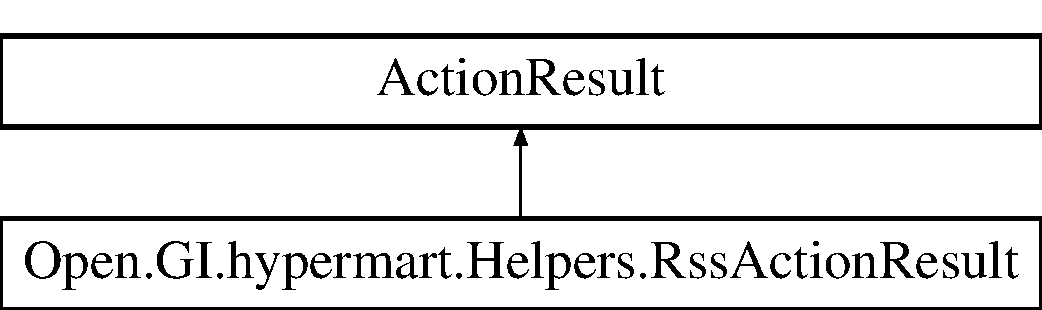
\includegraphics[height=2.000000cm]{class_open_1_1_g_i_1_1hypermart_1_1_helpers_1_1_rss_action_result}
\end{center}
\end{figure}
\subsection*{Public Member Functions}
\begin{DoxyCompactItemize}
\item 
override void \textbf{ Execute\+Result} (Controller\+Context context)
\begin{DoxyCompactList}\small\item\em Enables processing of the result of an action method by a custom type that inherits from the T\+:\+System.\+Web.\+Mvc.\+Action\+Result class. \end{DoxyCompactList}\end{DoxyCompactItemize}
\subsection*{Properties}
\begin{DoxyCompactItemize}
\item 
Syndication\+Feed \textbf{ Feed}\hspace{0.3cm}{\ttfamily  [get, set]}
\begin{DoxyCompactList}\small\item\em Gets or sets the feed. \end{DoxyCompactList}\end{DoxyCompactItemize}


\subsection{Detailed Description}
R\+SS Action Results 

\begin{DoxySeeAlso}{See also}
System.\+Web.\+Mvc.\+Action\+Result


\end{DoxySeeAlso}


Definition at line 43 of file Rss\+Action\+Result.\+cs.



\subsection{Member Function Documentation}
\mbox{\label{class_open_1_1_g_i_1_1hypermart_1_1_helpers_1_1_rss_action_result_a18ff30f679b2858b2d88a7dc267fd672}} 
\index{Open\+::\+G\+I\+::hypermart\+::\+Helpers\+::\+Rss\+Action\+Result@{Open\+::\+G\+I\+::hypermart\+::\+Helpers\+::\+Rss\+Action\+Result}!Execute\+Result@{Execute\+Result}}
\index{Execute\+Result@{Execute\+Result}!Open\+::\+G\+I\+::hypermart\+::\+Helpers\+::\+Rss\+Action\+Result@{Open\+::\+G\+I\+::hypermart\+::\+Helpers\+::\+Rss\+Action\+Result}}
\subsubsection{Execute\+Result()}
{\footnotesize\ttfamily override void Open.\+G\+I.\+hypermart.\+Helpers.\+Rss\+Action\+Result.\+Execute\+Result (\begin{DoxyParamCaption}\item[{Controller\+Context}]{context }\end{DoxyParamCaption})}



Enables processing of the result of an action method by a custom type that inherits from the T\+:\+System.\+Web.\+Mvc.\+Action\+Result class. 


\begin{DoxyParams}{Parameters}
{\em context} & The context in which the result is executed. The context information includes the controller, H\+T\+TP content, request context, and route data.\\
\hline
\end{DoxyParams}


Definition at line 57 of file Rss\+Action\+Result.\+cs.



\subsection{Property Documentation}
\mbox{\label{class_open_1_1_g_i_1_1hypermart_1_1_helpers_1_1_rss_action_result_a3b07cc4558b6a4863821fbedd9aa6888}} 
\index{Open\+::\+G\+I\+::hypermart\+::\+Helpers\+::\+Rss\+Action\+Result@{Open\+::\+G\+I\+::hypermart\+::\+Helpers\+::\+Rss\+Action\+Result}!Feed@{Feed}}
\index{Feed@{Feed}!Open\+::\+G\+I\+::hypermart\+::\+Helpers\+::\+Rss\+Action\+Result@{Open\+::\+G\+I\+::hypermart\+::\+Helpers\+::\+Rss\+Action\+Result}}
\subsubsection{Feed}
{\footnotesize\ttfamily Syndication\+Feed Open.\+G\+I.\+hypermart.\+Helpers.\+Rss\+Action\+Result.\+Feed\hspace{0.3cm}{\ttfamily [get]}, {\ttfamily [set]}}



Gets or sets the feed. 

The feed. 

Definition at line 51 of file Rss\+Action\+Result.\+cs.



The documentation for this class was generated from the following file\+:\begin{DoxyCompactItemize}
\item 
C\+:/\+Projects/\+App-\/\+Utility-\/\+Store/\+Open.\+G\+I.\+hypermart/\+Helpers/\textbf{ Rss\+Action\+Result.\+cs}\end{DoxyCompactItemize}

\hypertarget{class_open_1_1_g_i_1_1hypermart_1_1_models_1_1_screenshot}{}\section{Open.\+G\+I.\+hypermart.\+Models.\+Screenshot Class Reference}
\label{class_open_1_1_g_i_1_1hypermart_1_1_models_1_1_screenshot}\index{Open.\+G\+I.\+hypermart.\+Models.\+Screenshot@{Open.\+G\+I.\+hypermart.\+Models.\+Screenshot}}


Screen Shot Model Class  


\subsection*{Properties}
\begin{DoxyCompactItemize}
\item 
int \hyperlink{class_open_1_1_g_i_1_1hypermart_1_1_models_1_1_screenshot_a7460fabffe75a362966595c8b86cdef2}{ID}\hspace{0.3cm}{\ttfamily  \mbox{[}get, set\mbox{]}}
\begin{DoxyCompactList}\small\item\em Gets or sets the identifier. \end{DoxyCompactList}\item 
byte \mbox{[}$\,$\mbox{]} \hyperlink{class_open_1_1_g_i_1_1hypermart_1_1_models_1_1_screenshot_a435ca1863d66de2de497d603585610d8}{Screen\+Shot1}\hspace{0.3cm}{\ttfamily  \mbox{[}get, set\mbox{]}}
\begin{DoxyCompactList}\small\item\em Gets or sets the screen shot1. \end{DoxyCompactList}\item 
int \hyperlink{class_open_1_1_g_i_1_1hypermart_1_1_models_1_1_screenshot_ad381abf51bb0ebb1c2566c70df11c05a}{Product\+ID}\hspace{0.3cm}{\ttfamily  \mbox{[}get, set\mbox{]}}
\begin{DoxyCompactList}\small\item\em Gets or sets the product\+\_\+ identifier. \end{DoxyCompactList}\item 
\hyperlink{class_open_1_1_g_i_1_1hypermart_1_1_models_1_1_product}{Product} \hyperlink{class_open_1_1_g_i_1_1hypermart_1_1_models_1_1_screenshot_ae4e4b60e07136a6c4debe888426d6f6b}{Product}\hspace{0.3cm}{\ttfamily  \mbox{[}get, set\mbox{]}}
\begin{DoxyCompactList}\small\item\em Gets or sets the product. \end{DoxyCompactList}\item 
virtual \hyperlink{class_open_1_1_g_i_1_1hypermart_1_1_models_1_1_product}{Product} \hyperlink{class_open_1_1_g_i_1_1hypermart_1_1_models_1_1_screenshot_a8aed1d2289db7caefe8c7e14e0f5cc50}{Product}\hspace{0.3cm}{\ttfamily  \mbox{[}get, set\mbox{]}}
\end{DoxyCompactItemize}


\subsection{Detailed Description}
Screen Shot Model Class 



\subsection{Property Documentation}
\hypertarget{class_open_1_1_g_i_1_1hypermart_1_1_models_1_1_screenshot_a7460fabffe75a362966595c8b86cdef2}{}\label{class_open_1_1_g_i_1_1hypermart_1_1_models_1_1_screenshot_a7460fabffe75a362966595c8b86cdef2} 
\index{Open\+::\+G\+I\+::hypermart\+::\+Models\+::\+Screenshot@{Open\+::\+G\+I\+::hypermart\+::\+Models\+::\+Screenshot}!ID@{ID}}
\index{ID@{ID}!Open\+::\+G\+I\+::hypermart\+::\+Models\+::\+Screenshot@{Open\+::\+G\+I\+::hypermart\+::\+Models\+::\+Screenshot}}
\subsubsection{\texorpdfstring{ID}{ID}}
{\footnotesize\ttfamily int Open.\+G\+I.\+hypermart.\+Models.\+Screenshot.\+ID\hspace{0.3cm}{\ttfamily [get]}, {\ttfamily [set]}}



Gets or sets the identifier. 

The identifier. \hypertarget{class_open_1_1_g_i_1_1hypermart_1_1_models_1_1_screenshot_a8aed1d2289db7caefe8c7e14e0f5cc50}{}\label{class_open_1_1_g_i_1_1hypermart_1_1_models_1_1_screenshot_a8aed1d2289db7caefe8c7e14e0f5cc50} 
\index{Open\+::\+G\+I\+::hypermart\+::\+Models\+::\+Screenshot@{Open\+::\+G\+I\+::hypermart\+::\+Models\+::\+Screenshot}!Product@{Product}}
\index{Product@{Product}!Open\+::\+G\+I\+::hypermart\+::\+Models\+::\+Screenshot@{Open\+::\+G\+I\+::hypermart\+::\+Models\+::\+Screenshot}}
\subsubsection{\texorpdfstring{Product}{Product}\hspace{0.1cm}{\footnotesize\ttfamily [1/2]}}
{\footnotesize\ttfamily virtual \hyperlink{class_open_1_1_g_i_1_1hypermart_1_1_models_1_1_product}{Product} Open.\+G\+I.\+hypermart.\+Models.\+Screenshot.\+Product\hspace{0.3cm}{\ttfamily [get]}, {\ttfamily [set]}}

\hypertarget{class_open_1_1_g_i_1_1hypermart_1_1_models_1_1_screenshot_ae4e4b60e07136a6c4debe888426d6f6b}{}\label{class_open_1_1_g_i_1_1hypermart_1_1_models_1_1_screenshot_ae4e4b60e07136a6c4debe888426d6f6b} 
\index{Open\+::\+G\+I\+::hypermart\+::\+Models\+::\+Screenshot@{Open\+::\+G\+I\+::hypermart\+::\+Models\+::\+Screenshot}!Product@{Product}}
\index{Product@{Product}!Open\+::\+G\+I\+::hypermart\+::\+Models\+::\+Screenshot@{Open\+::\+G\+I\+::hypermart\+::\+Models\+::\+Screenshot}}
\subsubsection{\texorpdfstring{Product}{Product}\hspace{0.1cm}{\footnotesize\ttfamily [2/2]}}
{\footnotesize\ttfamily \hyperlink{class_open_1_1_g_i_1_1hypermart_1_1_models_1_1_product}{Product} Open.\+G\+I.\+hypermart.\+Models.\+Screenshot.\+Product\hspace{0.3cm}{\ttfamily [get]}, {\ttfamily [set]}}



Gets or sets the product. 

The product. \hypertarget{class_open_1_1_g_i_1_1hypermart_1_1_models_1_1_screenshot_ad381abf51bb0ebb1c2566c70df11c05a}{}\label{class_open_1_1_g_i_1_1hypermart_1_1_models_1_1_screenshot_ad381abf51bb0ebb1c2566c70df11c05a} 
\index{Open\+::\+G\+I\+::hypermart\+::\+Models\+::\+Screenshot@{Open\+::\+G\+I\+::hypermart\+::\+Models\+::\+Screenshot}!Product\+ID@{Product\+ID}}
\index{Product\+ID@{Product\+ID}!Open\+::\+G\+I\+::hypermart\+::\+Models\+::\+Screenshot@{Open\+::\+G\+I\+::hypermart\+::\+Models\+::\+Screenshot}}
\subsubsection{\texorpdfstring{Product\+ID}{ProductID}}
{\footnotesize\ttfamily int Open.\+G\+I.\+hypermart.\+Models.\+Screenshot.\+Product\+ID\hspace{0.3cm}{\ttfamily [get]}, {\ttfamily [set]}}



Gets or sets the product\+\_\+ identifier. 

The product\+\_\+ identifier. \hypertarget{class_open_1_1_g_i_1_1hypermart_1_1_models_1_1_screenshot_a435ca1863d66de2de497d603585610d8}{}\label{class_open_1_1_g_i_1_1hypermart_1_1_models_1_1_screenshot_a435ca1863d66de2de497d603585610d8} 
\index{Open\+::\+G\+I\+::hypermart\+::\+Models\+::\+Screenshot@{Open\+::\+G\+I\+::hypermart\+::\+Models\+::\+Screenshot}!Screen\+Shot1@{Screen\+Shot1}}
\index{Screen\+Shot1@{Screen\+Shot1}!Open\+::\+G\+I\+::hypermart\+::\+Models\+::\+Screenshot@{Open\+::\+G\+I\+::hypermart\+::\+Models\+::\+Screenshot}}
\subsubsection{\texorpdfstring{Screen\+Shot1}{ScreenShot1}}
{\footnotesize\ttfamily byte \mbox{[}$\,$\mbox{]} Open.\+G\+I.\+hypermart.\+Models.\+Screenshot.\+Screen\+Shot1\hspace{0.3cm}{\ttfamily [get]}, {\ttfamily [set]}}



Gets or sets the screen shot1. 

The screen shot1. 

The documentation for this class was generated from the following file\+:\begin{DoxyCompactItemize}
\item 
C\+:/\+Projects/\+App-\/\+Utility-\/\+Store/\+Open.\+G\+I.\+hypermart/\+Models/\hyperlink{_models_2_screenshot_8cs}{Screenshot.\+cs}\end{DoxyCompactItemize}

\section{Open.\+G\+I.\+hypermart.\+Areas.\+Help\+Page.\+Model\+Descriptions.\+Simple\+Type\+Model\+Description Class Reference}
\label{class_open_1_1_g_i_1_1hypermart_1_1_areas_1_1_help_page_1_1_model_descriptions_1_1_simple_type_model_description}\index{Open.\+G\+I.\+hypermart.\+Areas.\+Help\+Page.\+Model\+Descriptions.\+Simple\+Type\+Model\+Description@{Open.\+G\+I.\+hypermart.\+Areas.\+Help\+Page.\+Model\+Descriptions.\+Simple\+Type\+Model\+Description}}


 


Inheritance diagram for Open.\+G\+I.\+hypermart.\+Areas.\+Help\+Page.\+Model\+Descriptions.\+Simple\+Type\+Model\+Description\+:\begin{figure}[H]
\begin{center}
\leavevmode
\includegraphics[height=2.000000cm]{class_open_1_1_g_i_1_1hypermart_1_1_areas_1_1_help_page_1_1_model_descriptions_1_1_simple_type_model_description}
\end{center}
\end{figure}
\subsection*{Additional Inherited Members}


\subsection{Detailed Description}


\begin{DoxySeeAlso}{See also}
\doxyref{Open.\+G\+I.\+hypermart.\+Areas.\+Help\+Page.\+Model\+Descriptions.\+Model\+Description}{p.}{class_open_1_1_g_i_1_1hypermart_1_1_areas_1_1_help_page_1_1_model_descriptions_1_1_model_description}


\end{DoxySeeAlso}


Definition at line 7 of file Simple\+Type\+Model\+Description.\+cs.



The documentation for this class was generated from the following file\+:\begin{DoxyCompactItemize}
\item 
C\+:/\+Projects/\+App-\/\+Utility-\/\+Store/\+Open.\+G\+I.\+hypermart/\+Areas/\+Help\+Page/\+Model\+Descriptions/\textbf{ Simple\+Type\+Model\+Description.\+cs}\end{DoxyCompactItemize}

\hypertarget{class_open_1_1_g_i_1_1hypermart_1_1_status}{}\section{Open.\+G\+I.\+hypermart.\+Status Class Reference}
\label{class_open_1_1_g_i_1_1hypermart_1_1_status}\index{Open.\+G\+I.\+hypermart.\+Status@{Open.\+G\+I.\+hypermart.\+Status}}


Summary description for \hyperlink{class_open_1_1_g_i_1_1hypermart_1_1_status}{Status}  


Inheritance diagram for Open.\+G\+I.\+hypermart.\+Status\+:\begin{figure}[H]
\begin{center}
\leavevmode
\includegraphics[height=2.000000cm]{class_open_1_1_g_i_1_1hypermart_1_1_status}
\end{center}
\end{figure}
\subsection*{Public Member Functions}
\begin{DoxyCompactItemize}
\item 
string \hyperlink{class_open_1_1_g_i_1_1hypermart_1_1_status_a73a11d6869226091bd66017995dfabef}{Hello\+World} ()
\begin{DoxyCompactList}\small\item\em This is the Hello World method. \end{DoxyCompactList}\end{DoxyCompactItemize}


\subsection{Detailed Description}
Summary description for \hyperlink{class_open_1_1_g_i_1_1hypermart_1_1_status}{Status} 



Definition at line 17 of file Status.\+asmx.\+cs.



\subsection{Member Function Documentation}
\hypertarget{class_open_1_1_g_i_1_1hypermart_1_1_status_a73a11d6869226091bd66017995dfabef}{}\index{Open\+::\+G\+I\+::hypermart\+::\+Status@{Open\+::\+G\+I\+::hypermart\+::\+Status}!Hello\+World@{Hello\+World}}
\index{Hello\+World@{Hello\+World}!Open\+::\+G\+I\+::hypermart\+::\+Status@{Open\+::\+G\+I\+::hypermart\+::\+Status}}
\subsubsection[{Hello\+World()}]{\setlength{\rightskip}{0pt plus 5cm}string Open.\+G\+I.\+hypermart.\+Status.\+Hello\+World (
\begin{DoxyParamCaption}
{}
\end{DoxyParamCaption}
)}\label{class_open_1_1_g_i_1_1hypermart_1_1_status_a73a11d6869226091bd66017995dfabef}


This is the Hello World method. 

\begin{DoxyReturn}{Returns}

\end{DoxyReturn}


Definition at line 25 of file Status.\+asmx.\+cs.



The documentation for this class was generated from the following file\+:\begin{DoxyCompactItemize}
\item 
C\+:/\+Projects/\+App-\/\+Utility-\/\+Store/\+Open.\+G\+I.\+hypermart/\hyperlink{_status_8asmx_8cs}{Status.\+asmx.\+cs}\end{DoxyCompactItemize}

\hypertarget{class_open_1_1_g_i_1_1hypermart_1_1_controllers_1_1_store_content_controller}{}\section{Open.\+G\+I.\+hypermart.\+Controllers.\+Store\+Content\+Controller Class Reference}
\label{class_open_1_1_g_i_1_1hypermart_1_1_controllers_1_1_store_content_controller}\index{Open.\+G\+I.\+hypermart.\+Controllers.\+Store\+Content\+Controller@{Open.\+G\+I.\+hypermart.\+Controllers.\+Store\+Content\+Controller}}


This is the Open\+GI \hyperlink{namespace_open_1_1_g_i_1_1hypermart_1_1_controllers_1_1_a_p_i}{A\+PI} layer for interacting with the Store(\+Ading content etc). Some of the calls here relating to updates and creation will require a session token.  


Inheritance diagram for Open.\+G\+I.\+hypermart.\+Controllers.\+Store\+Content\+Controller\+:\begin{figure}[H]
\begin{center}
\leavevmode
\includegraphics[height=2.000000cm]{class_open_1_1_g_i_1_1hypermart_1_1_controllers_1_1_store_content_controller}
\end{center}
\end{figure}
\subsection*{Public Member Functions}
\begin{DoxyCompactItemize}
\item 
\hyperlink{class_open_1_1_g_i_1_1hypermart_1_1_controllers_1_1_store_content_controller_a01bad24ca04f869ec58d136ff35b2d13}{Store\+Content\+Controller} ()
\begin{DoxyCompactList}\small\item\em Initializes a new instance of the \hyperlink{class_open_1_1_g_i_1_1hypermart_1_1_controllers_1_1_store_content_controller}{Store\+Content\+Controller} class. \end{DoxyCompactList}\item 
\hyperlink{class_open_1_1_g_i_1_1hypermart_1_1_controllers_1_1_store_content_controller_ad8b3b3f13892bbb028eb21b7e240d7e2}{Store\+Content\+Controller} (\hyperlink{interface_open_1_1_g_i_1_1hypermart_1_1_d_a_l_1_1_i_hypermart_context}{I\+Hypermart\+Context} db\+Context)
\begin{DoxyCompactList}\small\item\em Initializes a new instance of the \hyperlink{class_open_1_1_g_i_1_1hypermart_1_1_controllers_1_1_store_content_controller}{Store\+Content\+Controller} class. \end{DoxyCompactList}\item 
I\+Queryable$<$ \hyperlink{class_open_1_1_g_i_1_1hypermart_1_1_data_transformation_objects_1_1_product_d_t_o}{Product\+D\+TO} $>$ \hyperlink{class_open_1_1_g_i_1_1hypermart_1_1_controllers_1_1_store_content_controller_ac0cf1a9777a6cb4978fbd1507dea8bbf}{Get\+All\+Products} ()
\begin{DoxyCompactList}\small\item\em Gets all products. \end{DoxyCompactList}\item 
\hyperlink{class_open_1_1_g_i_1_1hypermart_1_1_data_transformation_objects_1_1_product_d_t_o}{Product\+D\+TO} \hyperlink{class_open_1_1_g_i_1_1hypermart_1_1_controllers_1_1_store_content_controller_a4859d188d3e79898959e74538e832247}{Get\+Product} (int id)
\begin{DoxyCompactList}\small\item\em Gets a product. \end{DoxyCompactList}\item 
\hyperlink{class_open_1_1_g_i_1_1hypermart_1_1_data_transformation_objects_1_1_product_d_t_o}{Product\+D\+TO} \hyperlink{class_open_1_1_g_i_1_1hypermart_1_1_controllers_1_1_store_content_controller_ac11817b427cdc3139f1a1022791d9697}{Post\+Product} (\hyperlink{class_open_1_1_g_i_1_1hypermart_1_1_models_1_1_product}{Product} item\+To\+Add)
\begin{DoxyCompactList}\small\item\em Create a New Product \end{DoxyCompactList}\item 
bool \hyperlink{class_open_1_1_g_i_1_1hypermart_1_1_controllers_1_1_store_content_controller_a3e98139b9c8d95c6afb1bbe699aff201}{Delete\+Product} (\hyperlink{class_open_1_1_g_i_1_1hypermart_1_1_models_1_1_product}{Product} product\+To\+Delete)
\begin{DoxyCompactList}\small\item\em Deletes the product. \end{DoxyCompactList}\item 
void \hyperlink{class_open_1_1_g_i_1_1hypermart_1_1_controllers_1_1_store_content_controller_aee0d4040607c0d07828fc0d000135fcd}{Delete\+Product} (int Product\+ID)
\begin{DoxyCompactList}\small\item\em Deletes the product. \end{DoxyCompactList}\item 
List$<$ \hyperlink{class_open_1_1_g_i_1_1hypermart_1_1_data_transformation_objects_1_1_file_d_t_o}{File\+D\+TO} $>$ \hyperlink{class_open_1_1_g_i_1_1hypermart_1_1_controllers_1_1_store_content_controller_ae0b56b375fd34ca44fd3d7c32be04c04}{Get\+Files} (int id)
\begin{DoxyCompactList}\small\item\em Gets all files for a product. \end{DoxyCompactList}\item 
\hyperlink{class_open_1_1_g_i_1_1hypermart_1_1_data_transformation_objects_1_1_file_d_t_o}{File\+D\+TO} \hyperlink{class_open_1_1_g_i_1_1hypermart_1_1_controllers_1_1_store_content_controller_aeab9cb977ea719d1baa4610b3bc6a631}{Post\+Product\+File} (int Product\+ID, \hyperlink{class_open_1_1_g_i_1_1hypermart_1_1_models_1_1_file}{Open.\+G\+I.\+hypermart.\+Models.\+File} File\+To\+Add)
\begin{DoxyCompactList}\small\item\em Posts the product file. \end{DoxyCompactList}\item 
\hyperlink{class_open_1_1_g_i_1_1hypermart_1_1_data_transformation_objects_1_1_file_d_t_o}{File\+D\+TO} \hyperlink{class_open_1_1_g_i_1_1hypermart_1_1_controllers_1_1_store_content_controller_a36a438b2ab2cbb1d937b6a4c5bd8b17d}{Add\+File} (int Product\+ID, \hyperlink{class_open_1_1_g_i_1_1hypermart_1_1_models_1_1_file}{Open.\+G\+I.\+hypermart.\+Models.\+File} File\+To\+Add)
\begin{DoxyCompactList}\small\item\em Add A File to a product \end{DoxyCompactList}\item 
void \hyperlink{class_open_1_1_g_i_1_1hypermart_1_1_controllers_1_1_store_content_controller_a7c5b861d456ae7b592165634a07c6738}{Add\+Screen\+Shot} (int Product\+ID)
\begin{DoxyCompactList}\small\item\em Add a Screenshot to an Product \end{DoxyCompactList}\item 
void \hyperlink{class_open_1_1_g_i_1_1hypermart_1_1_controllers_1_1_store_content_controller_ae9be0167fa1b3e2f785c08e04b602bc1}{Post\+Ratings} (\hyperlink{class_open_1_1_g_i_1_1hypermart_1_1_data_transformation_objects_1_1_rating_information_d_t_o}{Rating\+Information\+D\+TO} Rating\+To\+Add)
\begin{DoxyCompactList}\small\item\em Create a New Product Rating \end{DoxyCompactList}\end{DoxyCompactItemize}


\subsection{Detailed Description}
This is the Open\+GI \hyperlink{namespace_open_1_1_g_i_1_1hypermart_1_1_controllers_1_1_a_p_i}{A\+PI} layer for interacting with the Store(\+Ading content etc). Some of the calls here relating to updates and creation will require a session token. 



\subsection{Constructor \& Destructor Documentation}
\hypertarget{class_open_1_1_g_i_1_1hypermart_1_1_controllers_1_1_store_content_controller_a01bad24ca04f869ec58d136ff35b2d13}{}\label{class_open_1_1_g_i_1_1hypermart_1_1_controllers_1_1_store_content_controller_a01bad24ca04f869ec58d136ff35b2d13} 
\index{Open\+::\+G\+I\+::hypermart\+::\+Controllers\+::\+Store\+Content\+Controller@{Open\+::\+G\+I\+::hypermart\+::\+Controllers\+::\+Store\+Content\+Controller}!Store\+Content\+Controller@{Store\+Content\+Controller}}
\index{Store\+Content\+Controller@{Store\+Content\+Controller}!Open\+::\+G\+I\+::hypermart\+::\+Controllers\+::\+Store\+Content\+Controller@{Open\+::\+G\+I\+::hypermart\+::\+Controllers\+::\+Store\+Content\+Controller}}
\subsubsection{\texorpdfstring{Store\+Content\+Controller()}{StoreContentController()}\hspace{0.1cm}{\footnotesize\ttfamily [1/2]}}
{\footnotesize\ttfamily Open.\+G\+I.\+hypermart.\+Controllers.\+Store\+Content\+Controller.\+Store\+Content\+Controller (\begin{DoxyParamCaption}{ }\end{DoxyParamCaption})}



Initializes a new instance of the \hyperlink{class_open_1_1_g_i_1_1hypermart_1_1_controllers_1_1_store_content_controller}{Store\+Content\+Controller} class. 

\hypertarget{class_open_1_1_g_i_1_1hypermart_1_1_controllers_1_1_store_content_controller_ad8b3b3f13892bbb028eb21b7e240d7e2}{}\label{class_open_1_1_g_i_1_1hypermart_1_1_controllers_1_1_store_content_controller_ad8b3b3f13892bbb028eb21b7e240d7e2} 
\index{Open\+::\+G\+I\+::hypermart\+::\+Controllers\+::\+Store\+Content\+Controller@{Open\+::\+G\+I\+::hypermart\+::\+Controllers\+::\+Store\+Content\+Controller}!Store\+Content\+Controller@{Store\+Content\+Controller}}
\index{Store\+Content\+Controller@{Store\+Content\+Controller}!Open\+::\+G\+I\+::hypermart\+::\+Controllers\+::\+Store\+Content\+Controller@{Open\+::\+G\+I\+::hypermart\+::\+Controllers\+::\+Store\+Content\+Controller}}
\subsubsection{\texorpdfstring{Store\+Content\+Controller()}{StoreContentController()}\hspace{0.1cm}{\footnotesize\ttfamily [2/2]}}
{\footnotesize\ttfamily Open.\+G\+I.\+hypermart.\+Controllers.\+Store\+Content\+Controller.\+Store\+Content\+Controller (\begin{DoxyParamCaption}\item[{\hyperlink{interface_open_1_1_g_i_1_1hypermart_1_1_d_a_l_1_1_i_hypermart_context}{I\+Hypermart\+Context}}]{db\+Context }\end{DoxyParamCaption})}



Initializes a new instance of the \hyperlink{class_open_1_1_g_i_1_1hypermart_1_1_controllers_1_1_store_content_controller}{Store\+Content\+Controller} class. 


\begin{DoxyParams}{Parameters}
{\em db\+Context} & The database context.\\
\hline
\end{DoxyParams}


\subsection{Member Function Documentation}
\hypertarget{class_open_1_1_g_i_1_1hypermart_1_1_controllers_1_1_store_content_controller_a36a438b2ab2cbb1d937b6a4c5bd8b17d}{}\label{class_open_1_1_g_i_1_1hypermart_1_1_controllers_1_1_store_content_controller_a36a438b2ab2cbb1d937b6a4c5bd8b17d} 
\index{Open\+::\+G\+I\+::hypermart\+::\+Controllers\+::\+Store\+Content\+Controller@{Open\+::\+G\+I\+::hypermart\+::\+Controllers\+::\+Store\+Content\+Controller}!Add\+File@{Add\+File}}
\index{Add\+File@{Add\+File}!Open\+::\+G\+I\+::hypermart\+::\+Controllers\+::\+Store\+Content\+Controller@{Open\+::\+G\+I\+::hypermart\+::\+Controllers\+::\+Store\+Content\+Controller}}
\subsubsection{\texorpdfstring{Add\+File()}{AddFile()}}
{\footnotesize\ttfamily \hyperlink{class_open_1_1_g_i_1_1hypermart_1_1_data_transformation_objects_1_1_file_d_t_o}{File\+D\+TO} Open.\+G\+I.\+hypermart.\+Controllers.\+Store\+Content\+Controller.\+Add\+File (\begin{DoxyParamCaption}\item[{int}]{Product\+ID,  }\item[{\hyperlink{class_open_1_1_g_i_1_1hypermart_1_1_models_1_1_file}{Open.\+G\+I.\+hypermart.\+Models.\+File}}]{File\+To\+Add }\end{DoxyParamCaption})}



Add A File to a product 


\begin{DoxyParams}{Parameters}
{\em Product\+ID} & \\
\hline
{\em File\+To\+Add} & \\
\hline
\end{DoxyParams}
\begin{DoxyReturn}{Returns}

\end{DoxyReturn}
\hypertarget{class_open_1_1_g_i_1_1hypermart_1_1_controllers_1_1_store_content_controller_a7c5b861d456ae7b592165634a07c6738}{}\label{class_open_1_1_g_i_1_1hypermart_1_1_controllers_1_1_store_content_controller_a7c5b861d456ae7b592165634a07c6738} 
\index{Open\+::\+G\+I\+::hypermart\+::\+Controllers\+::\+Store\+Content\+Controller@{Open\+::\+G\+I\+::hypermart\+::\+Controllers\+::\+Store\+Content\+Controller}!Add\+Screen\+Shot@{Add\+Screen\+Shot}}
\index{Add\+Screen\+Shot@{Add\+Screen\+Shot}!Open\+::\+G\+I\+::hypermart\+::\+Controllers\+::\+Store\+Content\+Controller@{Open\+::\+G\+I\+::hypermart\+::\+Controllers\+::\+Store\+Content\+Controller}}
\subsubsection{\texorpdfstring{Add\+Screen\+Shot()}{AddScreenShot()}}
{\footnotesize\ttfamily void Open.\+G\+I.\+hypermart.\+Controllers.\+Store\+Content\+Controller.\+Add\+Screen\+Shot (\begin{DoxyParamCaption}\item[{int}]{Product\+ID }\end{DoxyParamCaption})}



Add a Screenshot to an Product 


\begin{DoxyParams}{Parameters}
{\em Product\+ID} & \\
\hline
\end{DoxyParams}
\hypertarget{class_open_1_1_g_i_1_1hypermart_1_1_controllers_1_1_store_content_controller_a3e98139b9c8d95c6afb1bbe699aff201}{}\label{class_open_1_1_g_i_1_1hypermart_1_1_controllers_1_1_store_content_controller_a3e98139b9c8d95c6afb1bbe699aff201} 
\index{Open\+::\+G\+I\+::hypermart\+::\+Controllers\+::\+Store\+Content\+Controller@{Open\+::\+G\+I\+::hypermart\+::\+Controllers\+::\+Store\+Content\+Controller}!Delete\+Product@{Delete\+Product}}
\index{Delete\+Product@{Delete\+Product}!Open\+::\+G\+I\+::hypermart\+::\+Controllers\+::\+Store\+Content\+Controller@{Open\+::\+G\+I\+::hypermart\+::\+Controllers\+::\+Store\+Content\+Controller}}
\subsubsection{\texorpdfstring{Delete\+Product()}{DeleteProduct()}\hspace{0.1cm}{\footnotesize\ttfamily [1/2]}}
{\footnotesize\ttfamily bool Open.\+G\+I.\+hypermart.\+Controllers.\+Store\+Content\+Controller.\+Delete\+Product (\begin{DoxyParamCaption}\item[{\hyperlink{class_open_1_1_g_i_1_1hypermart_1_1_models_1_1_product}{Product}}]{product\+To\+Delete }\end{DoxyParamCaption})}



Deletes the product. 


\begin{DoxyParams}{Parameters}
{\em product\+To\+Delete} & The product to delete.\\
\hline
\end{DoxyParams}
\begin{DoxyReturn}{Returns}

\end{DoxyReturn}
\hypertarget{class_open_1_1_g_i_1_1hypermart_1_1_controllers_1_1_store_content_controller_aee0d4040607c0d07828fc0d000135fcd}{}\label{class_open_1_1_g_i_1_1hypermart_1_1_controllers_1_1_store_content_controller_aee0d4040607c0d07828fc0d000135fcd} 
\index{Open\+::\+G\+I\+::hypermart\+::\+Controllers\+::\+Store\+Content\+Controller@{Open\+::\+G\+I\+::hypermart\+::\+Controllers\+::\+Store\+Content\+Controller}!Delete\+Product@{Delete\+Product}}
\index{Delete\+Product@{Delete\+Product}!Open\+::\+G\+I\+::hypermart\+::\+Controllers\+::\+Store\+Content\+Controller@{Open\+::\+G\+I\+::hypermart\+::\+Controllers\+::\+Store\+Content\+Controller}}
\subsubsection{\texorpdfstring{Delete\+Product()}{DeleteProduct()}\hspace{0.1cm}{\footnotesize\ttfamily [2/2]}}
{\footnotesize\ttfamily void Open.\+G\+I.\+hypermart.\+Controllers.\+Store\+Content\+Controller.\+Delete\+Product (\begin{DoxyParamCaption}\item[{int}]{Product\+ID }\end{DoxyParamCaption})}



Deletes the product. 


\begin{DoxyParams}{Parameters}
{\em Product\+ID} & The product identifier.\\
\hline
\end{DoxyParams}
\hypertarget{class_open_1_1_g_i_1_1hypermart_1_1_controllers_1_1_store_content_controller_ac0cf1a9777a6cb4978fbd1507dea8bbf}{}\label{class_open_1_1_g_i_1_1hypermart_1_1_controllers_1_1_store_content_controller_ac0cf1a9777a6cb4978fbd1507dea8bbf} 
\index{Open\+::\+G\+I\+::hypermart\+::\+Controllers\+::\+Store\+Content\+Controller@{Open\+::\+G\+I\+::hypermart\+::\+Controllers\+::\+Store\+Content\+Controller}!Get\+All\+Products@{Get\+All\+Products}}
\index{Get\+All\+Products@{Get\+All\+Products}!Open\+::\+G\+I\+::hypermart\+::\+Controllers\+::\+Store\+Content\+Controller@{Open\+::\+G\+I\+::hypermart\+::\+Controllers\+::\+Store\+Content\+Controller}}
\subsubsection{\texorpdfstring{Get\+All\+Products()}{GetAllProducts()}}
{\footnotesize\ttfamily I\+Queryable$<$\hyperlink{class_open_1_1_g_i_1_1hypermart_1_1_data_transformation_objects_1_1_product_d_t_o}{Product\+D\+TO}$>$ Open.\+G\+I.\+hypermart.\+Controllers.\+Store\+Content\+Controller.\+Get\+All\+Products (\begin{DoxyParamCaption}{ }\end{DoxyParamCaption})}



Gets all products. 

\begin{DoxyReturn}{Returns}

\end{DoxyReturn}
\hypertarget{class_open_1_1_g_i_1_1hypermart_1_1_controllers_1_1_store_content_controller_ae0b56b375fd34ca44fd3d7c32be04c04}{}\label{class_open_1_1_g_i_1_1hypermart_1_1_controllers_1_1_store_content_controller_ae0b56b375fd34ca44fd3d7c32be04c04} 
\index{Open\+::\+G\+I\+::hypermart\+::\+Controllers\+::\+Store\+Content\+Controller@{Open\+::\+G\+I\+::hypermart\+::\+Controllers\+::\+Store\+Content\+Controller}!Get\+Files@{Get\+Files}}
\index{Get\+Files@{Get\+Files}!Open\+::\+G\+I\+::hypermart\+::\+Controllers\+::\+Store\+Content\+Controller@{Open\+::\+G\+I\+::hypermart\+::\+Controllers\+::\+Store\+Content\+Controller}}
\subsubsection{\texorpdfstring{Get\+Files()}{GetFiles()}}
{\footnotesize\ttfamily List$<$\hyperlink{class_open_1_1_g_i_1_1hypermart_1_1_data_transformation_objects_1_1_file_d_t_o}{File\+D\+TO}$>$ Open.\+G\+I.\+hypermart.\+Controllers.\+Store\+Content\+Controller.\+Get\+Files (\begin{DoxyParamCaption}\item[{int}]{id }\end{DoxyParamCaption})}



Gets all files for a product. 

\begin{DoxyReturn}{Returns}

\end{DoxyReturn}
\hypertarget{class_open_1_1_g_i_1_1hypermart_1_1_controllers_1_1_store_content_controller_a4859d188d3e79898959e74538e832247}{}\label{class_open_1_1_g_i_1_1hypermart_1_1_controllers_1_1_store_content_controller_a4859d188d3e79898959e74538e832247} 
\index{Open\+::\+G\+I\+::hypermart\+::\+Controllers\+::\+Store\+Content\+Controller@{Open\+::\+G\+I\+::hypermart\+::\+Controllers\+::\+Store\+Content\+Controller}!Get\+Product@{Get\+Product}}
\index{Get\+Product@{Get\+Product}!Open\+::\+G\+I\+::hypermart\+::\+Controllers\+::\+Store\+Content\+Controller@{Open\+::\+G\+I\+::hypermart\+::\+Controllers\+::\+Store\+Content\+Controller}}
\subsubsection{\texorpdfstring{Get\+Product()}{GetProduct()}}
{\footnotesize\ttfamily \hyperlink{class_open_1_1_g_i_1_1hypermart_1_1_data_transformation_objects_1_1_product_d_t_o}{Product\+D\+TO} Open.\+G\+I.\+hypermart.\+Controllers.\+Store\+Content\+Controller.\+Get\+Product (\begin{DoxyParamCaption}\item[{int}]{id }\end{DoxyParamCaption})}



Gets a product. 


\begin{DoxyParams}{Parameters}
{\em id} & The identifier.\\
\hline
\end{DoxyParams}
\begin{DoxyReturn}{Returns}

\end{DoxyReturn}

\begin{DoxyExceptions}{Exceptions}
{\em Http\+Response\+Exception} & \\
\hline
\end{DoxyExceptions}
\hypertarget{class_open_1_1_g_i_1_1hypermart_1_1_controllers_1_1_store_content_controller_ac11817b427cdc3139f1a1022791d9697}{}\label{class_open_1_1_g_i_1_1hypermart_1_1_controllers_1_1_store_content_controller_ac11817b427cdc3139f1a1022791d9697} 
\index{Open\+::\+G\+I\+::hypermart\+::\+Controllers\+::\+Store\+Content\+Controller@{Open\+::\+G\+I\+::hypermart\+::\+Controllers\+::\+Store\+Content\+Controller}!Post\+Product@{Post\+Product}}
\index{Post\+Product@{Post\+Product}!Open\+::\+G\+I\+::hypermart\+::\+Controllers\+::\+Store\+Content\+Controller@{Open\+::\+G\+I\+::hypermart\+::\+Controllers\+::\+Store\+Content\+Controller}}
\subsubsection{\texorpdfstring{Post\+Product()}{PostProduct()}}
{\footnotesize\ttfamily \hyperlink{class_open_1_1_g_i_1_1hypermart_1_1_data_transformation_objects_1_1_product_d_t_o}{Product\+D\+TO} Open.\+G\+I.\+hypermart.\+Controllers.\+Store\+Content\+Controller.\+Post\+Product (\begin{DoxyParamCaption}\item[{\hyperlink{class_open_1_1_g_i_1_1hypermart_1_1_models_1_1_product}{Product}}]{item\+To\+Add }\end{DoxyParamCaption})}



Create a New Product 

\hypertarget{class_open_1_1_g_i_1_1hypermart_1_1_controllers_1_1_store_content_controller_aeab9cb977ea719d1baa4610b3bc6a631}{}\label{class_open_1_1_g_i_1_1hypermart_1_1_controllers_1_1_store_content_controller_aeab9cb977ea719d1baa4610b3bc6a631} 
\index{Open\+::\+G\+I\+::hypermart\+::\+Controllers\+::\+Store\+Content\+Controller@{Open\+::\+G\+I\+::hypermart\+::\+Controllers\+::\+Store\+Content\+Controller}!Post\+Product\+File@{Post\+Product\+File}}
\index{Post\+Product\+File@{Post\+Product\+File}!Open\+::\+G\+I\+::hypermart\+::\+Controllers\+::\+Store\+Content\+Controller@{Open\+::\+G\+I\+::hypermart\+::\+Controllers\+::\+Store\+Content\+Controller}}
\subsubsection{\texorpdfstring{Post\+Product\+File()}{PostProductFile()}}
{\footnotesize\ttfamily \hyperlink{class_open_1_1_g_i_1_1hypermart_1_1_data_transformation_objects_1_1_file_d_t_o}{File\+D\+TO} Open.\+G\+I.\+hypermart.\+Controllers.\+Store\+Content\+Controller.\+Post\+Product\+File (\begin{DoxyParamCaption}\item[{int}]{Product\+ID,  }\item[{\hyperlink{class_open_1_1_g_i_1_1hypermart_1_1_models_1_1_file}{Open.\+G\+I.\+hypermart.\+Models.\+File}}]{File\+To\+Add }\end{DoxyParamCaption})}



Posts the product file. 


\begin{DoxyParams}{Parameters}
{\em Product\+ID} & The product identifier.\\
\hline
{\em File\+To\+Add} & The file to add.\\
\hline
\end{DoxyParams}
\begin{DoxyReturn}{Returns}

\end{DoxyReturn}

\begin{DoxyExceptions}{Exceptions}
{\em System.\+Web.\+Http.\+Http\+Response\+Exception} & \\
\hline
{\em System.\+Exception} & Cannot add a product file\\
\hline
\end{DoxyExceptions}
\hypertarget{class_open_1_1_g_i_1_1hypermart_1_1_controllers_1_1_store_content_controller_ae9be0167fa1b3e2f785c08e04b602bc1}{}\label{class_open_1_1_g_i_1_1hypermart_1_1_controllers_1_1_store_content_controller_ae9be0167fa1b3e2f785c08e04b602bc1} 
\index{Open\+::\+G\+I\+::hypermart\+::\+Controllers\+::\+Store\+Content\+Controller@{Open\+::\+G\+I\+::hypermart\+::\+Controllers\+::\+Store\+Content\+Controller}!Post\+Ratings@{Post\+Ratings}}
\index{Post\+Ratings@{Post\+Ratings}!Open\+::\+G\+I\+::hypermart\+::\+Controllers\+::\+Store\+Content\+Controller@{Open\+::\+G\+I\+::hypermart\+::\+Controllers\+::\+Store\+Content\+Controller}}
\subsubsection{\texorpdfstring{Post\+Ratings()}{PostRatings()}}
{\footnotesize\ttfamily void Open.\+G\+I.\+hypermart.\+Controllers.\+Store\+Content\+Controller.\+Post\+Ratings (\begin{DoxyParamCaption}\item[{\hyperlink{class_open_1_1_g_i_1_1hypermart_1_1_data_transformation_objects_1_1_rating_information_d_t_o}{Rating\+Information\+D\+TO}}]{Rating\+To\+Add }\end{DoxyParamCaption})}



Create a New Product Rating 



The documentation for this class was generated from the following file\+:\begin{DoxyCompactItemize}
\item 
C\+:/\+Projects/\+App-\/\+Utility-\/\+Store/\+Open.\+G\+I.\+hypermart/\+Controllers/\+A\+P\+I/\hyperlink{_store_content_controller_8cs}{Store\+Content\+Controller.\+cs}\end{DoxyCompactItemize}

\hypertarget{class_open_1_1_g_i_1_1hypermart_1_1_models_1_1_tag}{}\section{Open.\+G\+I.\+hypermart.\+Models.\+Tag Class Reference}
\label{class_open_1_1_g_i_1_1hypermart_1_1_models_1_1_tag}\index{Open.\+G\+I.\+hypermart.\+Models.\+Tag@{Open.\+G\+I.\+hypermart.\+Models.\+Tag}}


Hyper\+Mart -\/ Tagging. Tagging seems simple -\/ it is after all a collection of strings that the user can choose to asociate with a file.  


\subsection*{Properties}
\begin{DoxyCompactItemize}
\item 
string \hyperlink{class_open_1_1_g_i_1_1hypermart_1_1_models_1_1_tag_a9aa9f9231f2e67fc98403f5ae6be4c0c}{Name}\hspace{0.3cm}{\ttfamily  \mbox{[}get, set\mbox{]}}
\begin{DoxyCompactList}\small\item\em The \hyperlink{class_open_1_1_g_i_1_1hypermart_1_1_models_1_1_tag}{Tag} to save or associate with a file -\/ this might simplify to a Text collection (unsure) \end{DoxyCompactList}\end{DoxyCompactItemize}


\subsection{Detailed Description}
Hyper\+Mart -\/ Tagging. Tagging seems simple -\/ it is after all a collection of strings that the user can choose to asociate with a file. 



\subsection{Property Documentation}
\hypertarget{class_open_1_1_g_i_1_1hypermart_1_1_models_1_1_tag_a9aa9f9231f2e67fc98403f5ae6be4c0c}{}\label{class_open_1_1_g_i_1_1hypermart_1_1_models_1_1_tag_a9aa9f9231f2e67fc98403f5ae6be4c0c} 
\index{Open\+::\+G\+I\+::hypermart\+::\+Models\+::\+Tag@{Open\+::\+G\+I\+::hypermart\+::\+Models\+::\+Tag}!Name@{Name}}
\index{Name@{Name}!Open\+::\+G\+I\+::hypermart\+::\+Models\+::\+Tag@{Open\+::\+G\+I\+::hypermart\+::\+Models\+::\+Tag}}
\subsubsection{\texorpdfstring{Name}{Name}}
{\footnotesize\ttfamily string Open.\+G\+I.\+hypermart.\+Models.\+Tag.\+Name\hspace{0.3cm}{\ttfamily [get]}, {\ttfamily [set]}}



The \hyperlink{class_open_1_1_g_i_1_1hypermart_1_1_models_1_1_tag}{Tag} to save or associate with a file -\/ this might simplify to a Text collection (unsure) 



The documentation for this class was generated from the following file\+:\begin{DoxyCompactItemize}
\item 
C\+:/\+Projects/\+App-\/\+Utility-\/\+Store/\+Open.\+G\+I.\+hypermart/\+Models/\hyperlink{_tag_8cs}{Tag.\+cs}\end{DoxyCompactItemize}

\section{Open.\+G\+I.\+hypermart.\+Areas.\+Help\+Page.\+Text\+Sample Class Reference}
\label{class_open_1_1_g_i_1_1hypermart_1_1_areas_1_1_help_page_1_1_text_sample}\index{Open.\+G\+I.\+hypermart.\+Areas.\+Help\+Page.\+Text\+Sample@{Open.\+G\+I.\+hypermart.\+Areas.\+Help\+Page.\+Text\+Sample}}


This represents a preformatted text sample on the help page. There\textquotesingle{}s a display template named \doxyref{Text\+Sample}{p.}{class_open_1_1_g_i_1_1hypermart_1_1_areas_1_1_help_page_1_1_text_sample} associated with this class.  


\subsection*{Public Member Functions}
\begin{DoxyCompactItemize}
\item 
\textbf{ Text\+Sample} (string text)
\begin{DoxyCompactList}\small\item\em Initializes a new instance of the \doxyref{Text\+Sample}{p.}{class_open_1_1_g_i_1_1hypermart_1_1_areas_1_1_help_page_1_1_text_sample} class. \end{DoxyCompactList}\item 
override bool \textbf{ Equals} (object obj)
\begin{DoxyCompactList}\small\item\em Determines whether the specified System.\+Object, is equal to this instance. \end{DoxyCompactList}\item 
override int \textbf{ Get\+Hash\+Code} ()
\begin{DoxyCompactList}\small\item\em Returns a hash code for this instance. \end{DoxyCompactList}\item 
override string \textbf{ To\+String} ()
\begin{DoxyCompactList}\small\item\em Returns a System.\+String that represents this instance. \end{DoxyCompactList}\end{DoxyCompactItemize}
\subsection*{Properties}
\begin{DoxyCompactItemize}
\item 
string \textbf{ Text}\hspace{0.3cm}{\ttfamily  [get]}
\begin{DoxyCompactList}\small\item\em Gets the text. \end{DoxyCompactList}\end{DoxyCompactItemize}


\subsection{Detailed Description}
This represents a preformatted text sample on the help page. There\textquotesingle{}s a display template named \doxyref{Text\+Sample}{p.}{class_open_1_1_g_i_1_1hypermart_1_1_areas_1_1_help_page_1_1_text_sample} associated with this class. 



Definition at line 8 of file Text\+Sample.\+cs.



\subsection{Constructor \& Destructor Documentation}
\mbox{\label{class_open_1_1_g_i_1_1hypermart_1_1_areas_1_1_help_page_1_1_text_sample_aa2097f4582d638f73b4982201ab7e3e3}} 
\index{Open\+::\+G\+I\+::hypermart\+::\+Areas\+::\+Help\+Page\+::\+Text\+Sample@{Open\+::\+G\+I\+::hypermart\+::\+Areas\+::\+Help\+Page\+::\+Text\+Sample}!Text\+Sample@{Text\+Sample}}
\index{Text\+Sample@{Text\+Sample}!Open\+::\+G\+I\+::hypermart\+::\+Areas\+::\+Help\+Page\+::\+Text\+Sample@{Open\+::\+G\+I\+::hypermart\+::\+Areas\+::\+Help\+Page\+::\+Text\+Sample}}
\subsubsection{Text\+Sample()}
{\footnotesize\ttfamily Open.\+G\+I.\+hypermart.\+Areas.\+Help\+Page.\+Text\+Sample.\+Text\+Sample (\begin{DoxyParamCaption}\item[{string}]{text }\end{DoxyParamCaption})}



Initializes a new instance of the \doxyref{Text\+Sample}{p.}{class_open_1_1_g_i_1_1hypermart_1_1_areas_1_1_help_page_1_1_text_sample} class. 


\begin{DoxyParams}{Parameters}
{\em text} & The text.\\
\hline
\end{DoxyParams}

\begin{DoxyExceptions}{Exceptions}
{\em System.\+Argument\+Null\+Exception} & text\\
\hline
\end{DoxyExceptions}


Definition at line 15 of file Text\+Sample.\+cs.



\subsection{Member Function Documentation}
\mbox{\label{class_open_1_1_g_i_1_1hypermart_1_1_areas_1_1_help_page_1_1_text_sample_a05b2a9d64c25c827a041e83516b4cb18}} 
\index{Open\+::\+G\+I\+::hypermart\+::\+Areas\+::\+Help\+Page\+::\+Text\+Sample@{Open\+::\+G\+I\+::hypermart\+::\+Areas\+::\+Help\+Page\+::\+Text\+Sample}!Equals@{Equals}}
\index{Equals@{Equals}!Open\+::\+G\+I\+::hypermart\+::\+Areas\+::\+Help\+Page\+::\+Text\+Sample@{Open\+::\+G\+I\+::hypermart\+::\+Areas\+::\+Help\+Page\+::\+Text\+Sample}}
\subsubsection{Equals()}
{\footnotesize\ttfamily override bool Open.\+G\+I.\+hypermart.\+Areas.\+Help\+Page.\+Text\+Sample.\+Equals (\begin{DoxyParamCaption}\item[{object}]{obj }\end{DoxyParamCaption})}



Determines whether the specified System.\+Object, is equal to this instance. 


\begin{DoxyParams}{Parameters}
{\em obj} & The System.\+Object to compare with this instance.\\
\hline
\end{DoxyParams}
\begin{DoxyReturn}{Returns}
{\ttfamily true} if the specified System.\+Object is equal to this instance; otherwise, {\ttfamily false}. 
\end{DoxyReturn}


Definition at line 39 of file Text\+Sample.\+cs.

\mbox{\label{class_open_1_1_g_i_1_1hypermart_1_1_areas_1_1_help_page_1_1_text_sample_a020567c194ea1dff6b48f033c7dee994}} 
\index{Open\+::\+G\+I\+::hypermart\+::\+Areas\+::\+Help\+Page\+::\+Text\+Sample@{Open\+::\+G\+I\+::hypermart\+::\+Areas\+::\+Help\+Page\+::\+Text\+Sample}!Get\+Hash\+Code@{Get\+Hash\+Code}}
\index{Get\+Hash\+Code@{Get\+Hash\+Code}!Open\+::\+G\+I\+::hypermart\+::\+Areas\+::\+Help\+Page\+::\+Text\+Sample@{Open\+::\+G\+I\+::hypermart\+::\+Areas\+::\+Help\+Page\+::\+Text\+Sample}}
\subsubsection{Get\+Hash\+Code()}
{\footnotesize\ttfamily override int Open.\+G\+I.\+hypermart.\+Areas.\+Help\+Page.\+Text\+Sample.\+Get\+Hash\+Code (\begin{DoxyParamCaption}{ }\end{DoxyParamCaption})}



Returns a hash code for this instance. 

\begin{DoxyReturn}{Returns}
A hash code for this instance, suitable for use in hashing algorithms and data structures like a hash table. 
\end{DoxyReturn}


Definition at line 51 of file Text\+Sample.\+cs.

\mbox{\label{class_open_1_1_g_i_1_1hypermart_1_1_areas_1_1_help_page_1_1_text_sample_a06ee6af965d7778dcb62e1d49af71740}} 
\index{Open\+::\+G\+I\+::hypermart\+::\+Areas\+::\+Help\+Page\+::\+Text\+Sample@{Open\+::\+G\+I\+::hypermart\+::\+Areas\+::\+Help\+Page\+::\+Text\+Sample}!To\+String@{To\+String}}
\index{To\+String@{To\+String}!Open\+::\+G\+I\+::hypermart\+::\+Areas\+::\+Help\+Page\+::\+Text\+Sample@{Open\+::\+G\+I\+::hypermart\+::\+Areas\+::\+Help\+Page\+::\+Text\+Sample}}
\subsubsection{To\+String()}
{\footnotesize\ttfamily override string Open.\+G\+I.\+hypermart.\+Areas.\+Help\+Page.\+Text\+Sample.\+To\+String (\begin{DoxyParamCaption}{ }\end{DoxyParamCaption})}



Returns a System.\+String that represents this instance. 

\begin{DoxyReturn}{Returns}
A System.\+String that represents this instance. 
\end{DoxyReturn}


Definition at line 62 of file Text\+Sample.\+cs.



\subsection{Property Documentation}
\mbox{\label{class_open_1_1_g_i_1_1hypermart_1_1_areas_1_1_help_page_1_1_text_sample_aac44397744d5ca5d933bc1d85b07eda6}} 
\index{Open\+::\+G\+I\+::hypermart\+::\+Areas\+::\+Help\+Page\+::\+Text\+Sample@{Open\+::\+G\+I\+::hypermart\+::\+Areas\+::\+Help\+Page\+::\+Text\+Sample}!Text@{Text}}
\index{Text@{Text}!Open\+::\+G\+I\+::hypermart\+::\+Areas\+::\+Help\+Page\+::\+Text\+Sample@{Open\+::\+G\+I\+::hypermart\+::\+Areas\+::\+Help\+Page\+::\+Text\+Sample}}
\subsubsection{Text}
{\footnotesize\ttfamily string Open.\+G\+I.\+hypermart.\+Areas.\+Help\+Page.\+Text\+Sample.\+Text\hspace{0.3cm}{\ttfamily [get]}}



Gets the text. 

The text. 

Definition at line 30 of file Text\+Sample.\+cs.



The documentation for this class was generated from the following file\+:\begin{DoxyCompactItemize}
\item 
C\+:/\+Projects/\+App-\/\+Utility-\/\+Store/\+Open.\+G\+I.\+hypermart/\+Areas/\+Help\+Page/\+Sample\+Generation/\textbf{ Text\+Sample.\+cs}\end{DoxyCompactItemize}

\hypertarget{class_open_1_1_g_i_1_1hypermart_1_1_models_1_1_user}{}\section{Open.\+G\+I.\+hypermart.\+Models.\+User Class Reference}
\label{class_open_1_1_g_i_1_1hypermart_1_1_models_1_1_user}\index{Open.\+G\+I.\+hypermart.\+Models.\+User@{Open.\+G\+I.\+hypermart.\+Models.\+User}}


\hyperlink{class_open_1_1_g_i_1_1hypermart_1_1_models_1_1_user}{User} Model Class  


\subsection*{Properties}
\begin{DoxyCompactItemize}
\item 
string \hyperlink{class_open_1_1_g_i_1_1hypermart_1_1_models_1_1_user_a8681bb284b2bce5e87537a5dedc2dc05}{username}\hspace{0.3cm}{\ttfamily  \mbox{[}get, set\mbox{]}}
\begin{DoxyCompactList}\small\item\em Gets or sets the username. \end{DoxyCompactList}\item 
string \hyperlink{class_open_1_1_g_i_1_1hypermart_1_1_models_1_1_user_a70e545515c09bf8fc7a646c8f1a883a2}{Phone\+Numnber}\hspace{0.3cm}{\ttfamily  \mbox{[}get, set\mbox{]}}
\begin{DoxyCompactList}\small\item\em Gets or sets the phone numnber. \end{DoxyCompactList}\item 
Image \hyperlink{class_open_1_1_g_i_1_1hypermart_1_1_models_1_1_user_ae5b46912f2c2765d720a0a4754cc1921}{Photo}\hspace{0.3cm}{\ttfamily  \mbox{[}get, set\mbox{]}}
\begin{DoxyCompactList}\small\item\em Gets or sets the photo. \end{DoxyCompactList}\item 
string \hyperlink{class_open_1_1_g_i_1_1hypermart_1_1_models_1_1_user_a7b16ff0fd873d16ef921cd94f89be6f5}{Email}\hspace{0.3cm}{\ttfamily  \mbox{[}get, set\mbox{]}}
\begin{DoxyCompactList}\small\item\em Gets or sets the email. \end{DoxyCompactList}\item 
string \hyperlink{class_open_1_1_g_i_1_1hypermart_1_1_models_1_1_user_ad0aa7cba72b233858607496eb693d149}{Job\+Title}\hspace{0.3cm}{\ttfamily  \mbox{[}get, set\mbox{]}}
\begin{DoxyCompactList}\small\item\em Gets or sets the job title. \end{DoxyCompactList}\end{DoxyCompactItemize}


\subsection{Detailed Description}
\hyperlink{class_open_1_1_g_i_1_1hypermart_1_1_models_1_1_user}{User} Model Class 



\subsection{Property Documentation}
\hypertarget{class_open_1_1_g_i_1_1hypermart_1_1_models_1_1_user_a7b16ff0fd873d16ef921cd94f89be6f5}{}\label{class_open_1_1_g_i_1_1hypermart_1_1_models_1_1_user_a7b16ff0fd873d16ef921cd94f89be6f5} 
\index{Open\+::\+G\+I\+::hypermart\+::\+Models\+::\+User@{Open\+::\+G\+I\+::hypermart\+::\+Models\+::\+User}!Email@{Email}}
\index{Email@{Email}!Open\+::\+G\+I\+::hypermart\+::\+Models\+::\+User@{Open\+::\+G\+I\+::hypermart\+::\+Models\+::\+User}}
\subsubsection{\texorpdfstring{Email}{Email}}
{\footnotesize\ttfamily string Open.\+G\+I.\+hypermart.\+Models.\+User.\+Email\hspace{0.3cm}{\ttfamily [get]}, {\ttfamily [set]}}



Gets or sets the email. 

The email. \hypertarget{class_open_1_1_g_i_1_1hypermart_1_1_models_1_1_user_ad0aa7cba72b233858607496eb693d149}{}\label{class_open_1_1_g_i_1_1hypermart_1_1_models_1_1_user_ad0aa7cba72b233858607496eb693d149} 
\index{Open\+::\+G\+I\+::hypermart\+::\+Models\+::\+User@{Open\+::\+G\+I\+::hypermart\+::\+Models\+::\+User}!Job\+Title@{Job\+Title}}
\index{Job\+Title@{Job\+Title}!Open\+::\+G\+I\+::hypermart\+::\+Models\+::\+User@{Open\+::\+G\+I\+::hypermart\+::\+Models\+::\+User}}
\subsubsection{\texorpdfstring{Job\+Title}{JobTitle}}
{\footnotesize\ttfamily string Open.\+G\+I.\+hypermart.\+Models.\+User.\+Job\+Title\hspace{0.3cm}{\ttfamily [get]}, {\ttfamily [set]}}



Gets or sets the job title. 

The job title. \hypertarget{class_open_1_1_g_i_1_1hypermart_1_1_models_1_1_user_a70e545515c09bf8fc7a646c8f1a883a2}{}\label{class_open_1_1_g_i_1_1hypermart_1_1_models_1_1_user_a70e545515c09bf8fc7a646c8f1a883a2} 
\index{Open\+::\+G\+I\+::hypermart\+::\+Models\+::\+User@{Open\+::\+G\+I\+::hypermart\+::\+Models\+::\+User}!Phone\+Numnber@{Phone\+Numnber}}
\index{Phone\+Numnber@{Phone\+Numnber}!Open\+::\+G\+I\+::hypermart\+::\+Models\+::\+User@{Open\+::\+G\+I\+::hypermart\+::\+Models\+::\+User}}
\subsubsection{\texorpdfstring{Phone\+Numnber}{PhoneNumnber}}
{\footnotesize\ttfamily string Open.\+G\+I.\+hypermart.\+Models.\+User.\+Phone\+Numnber\hspace{0.3cm}{\ttfamily [get]}, {\ttfamily [set]}}



Gets or sets the phone numnber. 

The phone numnber. \hypertarget{class_open_1_1_g_i_1_1hypermart_1_1_models_1_1_user_ae5b46912f2c2765d720a0a4754cc1921}{}\label{class_open_1_1_g_i_1_1hypermart_1_1_models_1_1_user_ae5b46912f2c2765d720a0a4754cc1921} 
\index{Open\+::\+G\+I\+::hypermart\+::\+Models\+::\+User@{Open\+::\+G\+I\+::hypermart\+::\+Models\+::\+User}!Photo@{Photo}}
\index{Photo@{Photo}!Open\+::\+G\+I\+::hypermart\+::\+Models\+::\+User@{Open\+::\+G\+I\+::hypermart\+::\+Models\+::\+User}}
\subsubsection{\texorpdfstring{Photo}{Photo}}
{\footnotesize\ttfamily Image Open.\+G\+I.\+hypermart.\+Models.\+User.\+Photo\hspace{0.3cm}{\ttfamily [get]}, {\ttfamily [set]}}



Gets or sets the photo. 

The photo. \hypertarget{class_open_1_1_g_i_1_1hypermart_1_1_models_1_1_user_a8681bb284b2bce5e87537a5dedc2dc05}{}\label{class_open_1_1_g_i_1_1hypermart_1_1_models_1_1_user_a8681bb284b2bce5e87537a5dedc2dc05} 
\index{Open\+::\+G\+I\+::hypermart\+::\+Models\+::\+User@{Open\+::\+G\+I\+::hypermart\+::\+Models\+::\+User}!username@{username}}
\index{username@{username}!Open\+::\+G\+I\+::hypermart\+::\+Models\+::\+User@{Open\+::\+G\+I\+::hypermart\+::\+Models\+::\+User}}
\subsubsection{\texorpdfstring{username}{username}}
{\footnotesize\ttfamily string Open.\+G\+I.\+hypermart.\+Models.\+User.\+username\hspace{0.3cm}{\ttfamily [get]}, {\ttfamily [set]}}



Gets or sets the username. 

The username. 

The documentation for this class was generated from the following file\+:\begin{DoxyCompactItemize}
\item 
C\+:/\+Projects/\+App-\/\+Utility-\/\+Store/\+Open.\+G\+I.\+hypermart/\+Models/\hyperlink{_models_2_user_8cs}{User.\+cs}\end{DoxyCompactItemize}

\hypertarget{class_open_1_1_g_i_1_1hypermart_1_1_controllers_1_1_a_p_i_1_1_user_controller}{}\section{Open.\+G\+I.\+hypermart.\+Controllers.\+A\+P\+I.\+User\+Controller Class Reference}
\label{class_open_1_1_g_i_1_1hypermart_1_1_controllers_1_1_a_p_i_1_1_user_controller}\index{Open.\+G\+I.\+hypermart.\+Controllers.\+A\+P\+I.\+User\+Controller@{Open.\+G\+I.\+hypermart.\+Controllers.\+A\+P\+I.\+User\+Controller}}


This is the Open\+GI \hyperlink{namespace_open_1_1_g_i_1_1hypermart_1_1_controllers_1_1_a_p_i}{A\+PI} layer for interacting with users. This \hyperlink{namespace_open_1_1_g_i_1_1hypermart_1_1_controllers_1_1_a_p_i}{A\+PI} layer allows user details to be retireved from Active Directory.  


Inheritance diagram for Open.\+G\+I.\+hypermart.\+Controllers.\+A\+P\+I.\+User\+Controller\+:\begin{figure}[H]
\begin{center}
\leavevmode
\includegraphics[height=2.000000cm]{class_open_1_1_g_i_1_1hypermart_1_1_controllers_1_1_a_p_i_1_1_user_controller}
\end{center}
\end{figure}
\subsection*{Public Member Functions}
\begin{DoxyCompactItemize}
\item 
\hyperlink{class_open_1_1_g_i_1_1hypermart_1_1_data_transformation_objects_1_1_user_d_t_o}{User\+D\+TO} \hyperlink{class_open_1_1_g_i_1_1hypermart_1_1_controllers_1_1_a_p_i_1_1_user_controller_af2896a942d750bcc948228c298221f15}{Details} (string userid)
\begin{DoxyCompactList}\small\item\em Retrieves the user information from the directory. \end{DoxyCompactList}\end{DoxyCompactItemize}


\subsection{Detailed Description}
This is the Open\+GI \hyperlink{namespace_open_1_1_g_i_1_1hypermart_1_1_controllers_1_1_a_p_i}{A\+PI} layer for interacting with users. This \hyperlink{namespace_open_1_1_g_i_1_1hypermart_1_1_controllers_1_1_a_p_i}{A\+PI} layer allows user details to be retireved from Active Directory. 

Required minimal configuration, but does require a directory services of sorts -\/ this should work with the Active Directory Lightweight Directory Services (to be confirmed). 

\subsection{Member Function Documentation}
\hypertarget{class_open_1_1_g_i_1_1hypermart_1_1_controllers_1_1_a_p_i_1_1_user_controller_af2896a942d750bcc948228c298221f15}{}\label{class_open_1_1_g_i_1_1hypermart_1_1_controllers_1_1_a_p_i_1_1_user_controller_af2896a942d750bcc948228c298221f15} 
\index{Open\+::\+G\+I\+::hypermart\+::\+Controllers\+::\+A\+P\+I\+::\+User\+Controller@{Open\+::\+G\+I\+::hypermart\+::\+Controllers\+::\+A\+P\+I\+::\+User\+Controller}!Details@{Details}}
\index{Details@{Details}!Open\+::\+G\+I\+::hypermart\+::\+Controllers\+::\+A\+P\+I\+::\+User\+Controller@{Open\+::\+G\+I\+::hypermart\+::\+Controllers\+::\+A\+P\+I\+::\+User\+Controller}}
\subsubsection{\texorpdfstring{Details()}{Details()}}
{\footnotesize\ttfamily \hyperlink{class_open_1_1_g_i_1_1hypermart_1_1_data_transformation_objects_1_1_user_d_t_o}{User\+D\+TO} Open.\+G\+I.\+hypermart.\+Controllers.\+A\+P\+I.\+User\+Controller.\+Details (\begin{DoxyParamCaption}\item[{string}]{userid }\end{DoxyParamCaption})}



Retrieves the user information from the directory. 


\begin{DoxyParams}{Parameters}
{\em userid} & \\
\hline
\end{DoxyParams}
\begin{DoxyReturn}{Returns}

\end{DoxyReturn}


The documentation for this class was generated from the following file\+:\begin{DoxyCompactItemize}
\item 
C\+:/\+Projects/\+App-\/\+Utility-\/\+Store/\+Open.\+G\+I.\+hypermart/\+Controllers/\+A\+P\+I/\hyperlink{_a_p_i_2_user_controller_8cs}{User\+Controller.\+cs}\end{DoxyCompactItemize}

\hypertarget{class_open_1_1_g_i_1_1hypermart_1_1_controllers_1_1_user_controller}{}\section{Open.\+G\+I.\+hypermart.\+Controllers.\+User\+Controller Class Reference}
\label{class_open_1_1_g_i_1_1hypermart_1_1_controllers_1_1_user_controller}\index{Open.\+G\+I.\+hypermart.\+Controllers.\+User\+Controller@{Open.\+G\+I.\+hypermart.\+Controllers.\+User\+Controller}}


User Controller  


Inheritance diagram for Open.\+G\+I.\+hypermart.\+Controllers.\+User\+Controller\+:\begin{figure}[H]
\begin{center}
\leavevmode
\includegraphics[height=2.000000cm]{class_open_1_1_g_i_1_1hypermart_1_1_controllers_1_1_user_controller}
\end{center}
\end{figure}
\subsection*{Public Member Functions}
\begin{DoxyCompactItemize}
\item 
Action\+Result \hyperlink{class_open_1_1_g_i_1_1hypermart_1_1_controllers_1_1_user_controller_a4627a7a94b713760f00050bac936a54f}{Details} (string id)
\begin{DoxyCompactList}\small\item\em Detailses the specified userid. \end{DoxyCompactList}\item 
Action\+Result \hyperlink{class_open_1_1_g_i_1_1hypermart_1_1_controllers_1_1_user_controller_a3168162b86edbdbd30a593fa6aca8e9f}{popup\+\_\+\+Details} (string userid)
\begin{DoxyCompactList}\small\item\em Detailses the specified userid. \end{DoxyCompactList}\end{DoxyCompactItemize}


\subsection{Detailed Description}
User Controller 

\begin{DoxySeeAlso}{See also}
System.\+Web.\+Mvc.\+Controller


\end{DoxySeeAlso}


\subsection{Member Function Documentation}
\hypertarget{class_open_1_1_g_i_1_1hypermart_1_1_controllers_1_1_user_controller_a4627a7a94b713760f00050bac936a54f}{}\label{class_open_1_1_g_i_1_1hypermart_1_1_controllers_1_1_user_controller_a4627a7a94b713760f00050bac936a54f} 
\index{Open\+::\+G\+I\+::hypermart\+::\+Controllers\+::\+User\+Controller@{Open\+::\+G\+I\+::hypermart\+::\+Controllers\+::\+User\+Controller}!Details@{Details}}
\index{Details@{Details}!Open\+::\+G\+I\+::hypermart\+::\+Controllers\+::\+User\+Controller@{Open\+::\+G\+I\+::hypermart\+::\+Controllers\+::\+User\+Controller}}
\subsubsection{\texorpdfstring{Details()}{Details()}}
{\footnotesize\ttfamily Action\+Result Open.\+G\+I.\+hypermart.\+Controllers.\+User\+Controller.\+Details (\begin{DoxyParamCaption}\item[{string}]{id }\end{DoxyParamCaption})}



Detailses the specified userid. 


\begin{DoxyParams}{Parameters}
{\em id} & The userid.\\
\hline
\end{DoxyParams}
\begin{DoxyReturn}{Returns}

\end{DoxyReturn}
\hypertarget{class_open_1_1_g_i_1_1hypermart_1_1_controllers_1_1_user_controller_a3168162b86edbdbd30a593fa6aca8e9f}{}\label{class_open_1_1_g_i_1_1hypermart_1_1_controllers_1_1_user_controller_a3168162b86edbdbd30a593fa6aca8e9f} 
\index{Open\+::\+G\+I\+::hypermart\+::\+Controllers\+::\+User\+Controller@{Open\+::\+G\+I\+::hypermart\+::\+Controllers\+::\+User\+Controller}!popup\+\_\+\+Details@{popup\+\_\+\+Details}}
\index{popup\+\_\+\+Details@{popup\+\_\+\+Details}!Open\+::\+G\+I\+::hypermart\+::\+Controllers\+::\+User\+Controller@{Open\+::\+G\+I\+::hypermart\+::\+Controllers\+::\+User\+Controller}}
\subsubsection{\texorpdfstring{popup\+\_\+\+Details()}{popup\_Details()}}
{\footnotesize\ttfamily Action\+Result Open.\+G\+I.\+hypermart.\+Controllers.\+User\+Controller.\+popup\+\_\+\+Details (\begin{DoxyParamCaption}\item[{string}]{userid }\end{DoxyParamCaption})}



Detailses the specified userid. 


\begin{DoxyParams}{Parameters}
{\em userid} & The userid.\\
\hline
\end{DoxyParams}
\begin{DoxyReturn}{Returns}

\end{DoxyReturn}


The documentation for this class was generated from the following file\+:\begin{DoxyCompactItemize}
\item 
C\+:/\+Projects/\+App-\/\+Utility-\/\+Store/\+Open.\+G\+I.\+hypermart/\+Controllers/\hyperlink{_user_controller_8cs}{User\+Controller.\+cs}\end{DoxyCompactItemize}

\hypertarget{class_open_1_1_g_i_1_1hypermart_1_1_data_transformation_objects_1_1_user_d_t_o}{}\section{Open.\+G\+I.\+hypermart.\+Data\+Transformation\+Objects.\+User\+D\+T\+O Class Reference}
\label{class_open_1_1_g_i_1_1hypermart_1_1_data_transformation_objects_1_1_user_d_t_o}\index{Open.\+G\+I.\+hypermart.\+Data\+Transformation\+Objects.\+User\+D\+T\+O@{Open.\+G\+I.\+hypermart.\+Data\+Transformation\+Objects.\+User\+D\+T\+O}}


Class for Over-\/the-\/wire transmission of user information. If a user cannot be found, then an Unknown User will be returned.  


\subsection*{Public Member Functions}
\begin{DoxyCompactItemize}
\item 
\hyperlink{class_open_1_1_g_i_1_1hypermart_1_1_data_transformation_objects_1_1_user_d_t_o_ab715e6cac8b432f39c5fe6f22e3db645}{User\+D\+T\+O} ()
\begin{DoxyCompactList}\small\item\em Initializes a new instance of the \hyperlink{class_open_1_1_g_i_1_1hypermart_1_1_data_transformation_objects_1_1_user_d_t_o}{User\+D\+T\+O} class. \end{DoxyCompactList}\item 
\hyperlink{class_open_1_1_g_i_1_1hypermart_1_1_data_transformation_objects_1_1_user_d_t_o_a21ce2f8eaac0781bcc484f8eeca38404}{User\+D\+T\+O} (\hyperlink{class_open_1_1_g_i_1_1hypermart_1_1_models_1_1_user}{Open.\+G\+I.\+hypermart.\+Models.\+User} User\+To\+Wrap)
\begin{DoxyCompactList}\small\item\em Initializes a new instance of the \hyperlink{class_open_1_1_g_i_1_1hypermart_1_1_data_transformation_objects_1_1_user_d_t_o}{User\+D\+T\+O} class. \end{DoxyCompactList}\end{DoxyCompactItemize}
\subsection*{Properties}
\begin{DoxyCompactItemize}
\item 
string \hyperlink{class_open_1_1_g_i_1_1hypermart_1_1_data_transformation_objects_1_1_user_d_t_o_a123512619de906f987a3da0b7ec32bb1}{username}\hspace{0.3cm}{\ttfamily  \mbox{[}get, set\mbox{]}}
\begin{DoxyCompactList}\small\item\em Gets or sets the username. \end{DoxyCompactList}\item 
string \hyperlink{class_open_1_1_g_i_1_1hypermart_1_1_data_transformation_objects_1_1_user_d_t_o_a8ead06f70fbd3e0bcc72bf3aaae4fc9f}{Phone\+Numnber}\hspace{0.3cm}{\ttfamily  \mbox{[}get, set\mbox{]}}
\begin{DoxyCompactList}\small\item\em Gets or sets the phone numnber. \end{DoxyCompactList}\item 
Byte\mbox{[}$\,$\mbox{]} \hyperlink{class_open_1_1_g_i_1_1hypermart_1_1_data_transformation_objects_1_1_user_d_t_o_a3e4447b4cd2ef861c95c1e9162cbceb1}{Photo\+\_\+byte\+Array}\hspace{0.3cm}{\ttfamily  \mbox{[}get, set\mbox{]}}
\begin{DoxyCompactList}\small\item\em Base 64 encoded png image. \end{DoxyCompactList}\item 
string \hyperlink{class_open_1_1_g_i_1_1hypermart_1_1_data_transformation_objects_1_1_user_d_t_o_a96fdfcc9b2aa36fb35f6612b9e99b535}{Email}\hspace{0.3cm}{\ttfamily  \mbox{[}get, set\mbox{]}}
\begin{DoxyCompactList}\small\item\em Gets or sets the email. \end{DoxyCompactList}\item 
string \hyperlink{class_open_1_1_g_i_1_1hypermart_1_1_data_transformation_objects_1_1_user_d_t_o_a7a436dea35ee6683f2f7f0c3e9551d08}{Job\+Title}\hspace{0.3cm}{\ttfamily  \mbox{[}get, set\mbox{]}}
\begin{DoxyCompactList}\small\item\em Gets or sets the job title. \end{DoxyCompactList}\end{DoxyCompactItemize}


\subsection{Detailed Description}
Class for Over-\/the-\/wire transmission of user information. If a user cannot be found, then an Unknown User will be returned. 



Definition at line 14 of file User\+D\+T\+O.\+cs.



\subsection{Constructor \& Destructor Documentation}
\hypertarget{class_open_1_1_g_i_1_1hypermart_1_1_data_transformation_objects_1_1_user_d_t_o_ab715e6cac8b432f39c5fe6f22e3db645}{}\index{Open\+::\+G\+I\+::hypermart\+::\+Data\+Transformation\+Objects\+::\+User\+D\+T\+O@{Open\+::\+G\+I\+::hypermart\+::\+Data\+Transformation\+Objects\+::\+User\+D\+T\+O}!User\+D\+T\+O@{User\+D\+T\+O}}
\index{User\+D\+T\+O@{User\+D\+T\+O}!Open\+::\+G\+I\+::hypermart\+::\+Data\+Transformation\+Objects\+::\+User\+D\+T\+O@{Open\+::\+G\+I\+::hypermart\+::\+Data\+Transformation\+Objects\+::\+User\+D\+T\+O}}
\subsubsection[{User\+D\+T\+O()}]{\setlength{\rightskip}{0pt plus 5cm}Open.\+G\+I.\+hypermart.\+Data\+Transformation\+Objects.\+User\+D\+T\+O.\+User\+D\+T\+O (
\begin{DoxyParamCaption}
{}
\end{DoxyParamCaption}
)}\label{class_open_1_1_g_i_1_1hypermart_1_1_data_transformation_objects_1_1_user_d_t_o_ab715e6cac8b432f39c5fe6f22e3db645}


Initializes a new instance of the \hyperlink{class_open_1_1_g_i_1_1hypermart_1_1_data_transformation_objects_1_1_user_d_t_o}{User\+D\+T\+O} class. 



Definition at line 19 of file User\+D\+T\+O.\+cs.

\hypertarget{class_open_1_1_g_i_1_1hypermart_1_1_data_transformation_objects_1_1_user_d_t_o_a21ce2f8eaac0781bcc484f8eeca38404}{}\index{Open\+::\+G\+I\+::hypermart\+::\+Data\+Transformation\+Objects\+::\+User\+D\+T\+O@{Open\+::\+G\+I\+::hypermart\+::\+Data\+Transformation\+Objects\+::\+User\+D\+T\+O}!User\+D\+T\+O@{User\+D\+T\+O}}
\index{User\+D\+T\+O@{User\+D\+T\+O}!Open\+::\+G\+I\+::hypermart\+::\+Data\+Transformation\+Objects\+::\+User\+D\+T\+O@{Open\+::\+G\+I\+::hypermart\+::\+Data\+Transformation\+Objects\+::\+User\+D\+T\+O}}
\subsubsection[{User\+D\+T\+O(\+Open.\+G\+I.\+hypermart.\+Models.\+User User\+To\+Wrap)}]{\setlength{\rightskip}{0pt plus 5cm}Open.\+G\+I.\+hypermart.\+Data\+Transformation\+Objects.\+User\+D\+T\+O.\+User\+D\+T\+O (
\begin{DoxyParamCaption}
\item[{{\bf Open.\+G\+I.\+hypermart.\+Models.\+User}}]{User\+To\+Wrap}
\end{DoxyParamCaption}
)}\label{class_open_1_1_g_i_1_1hypermart_1_1_data_transformation_objects_1_1_user_d_t_o_a21ce2f8eaac0781bcc484f8eeca38404}


Initializes a new instance of the \hyperlink{class_open_1_1_g_i_1_1hypermart_1_1_data_transformation_objects_1_1_user_d_t_o}{User\+D\+T\+O} class. 


\begin{DoxyParams}{Parameters}
{\em User\+To\+Wrap} & The user to wrap.\\
\hline
\end{DoxyParams}


Definition at line 28 of file User\+D\+T\+O.\+cs.



\subsection{Property Documentation}
\hypertarget{class_open_1_1_g_i_1_1hypermart_1_1_data_transformation_objects_1_1_user_d_t_o_a96fdfcc9b2aa36fb35f6612b9e99b535}{}\index{Open\+::\+G\+I\+::hypermart\+::\+Data\+Transformation\+Objects\+::\+User\+D\+T\+O@{Open\+::\+G\+I\+::hypermart\+::\+Data\+Transformation\+Objects\+::\+User\+D\+T\+O}!Email@{Email}}
\index{Email@{Email}!Open\+::\+G\+I\+::hypermart\+::\+Data\+Transformation\+Objects\+::\+User\+D\+T\+O@{Open\+::\+G\+I\+::hypermart\+::\+Data\+Transformation\+Objects\+::\+User\+D\+T\+O}}
\subsubsection[{Email}]{\setlength{\rightskip}{0pt plus 5cm}string Open.\+G\+I.\+hypermart.\+Data\+Transformation\+Objects.\+User\+D\+T\+O.\+Email\hspace{0.3cm}{\ttfamily [get]}, {\ttfamily [set]}}\label{class_open_1_1_g_i_1_1hypermart_1_1_data_transformation_objects_1_1_user_d_t_o_a96fdfcc9b2aa36fb35f6612b9e99b535}


Gets or sets the email. 

The email. 

Definition at line 60 of file User\+D\+T\+O.\+cs.

\hypertarget{class_open_1_1_g_i_1_1hypermart_1_1_data_transformation_objects_1_1_user_d_t_o_a7a436dea35ee6683f2f7f0c3e9551d08}{}\index{Open\+::\+G\+I\+::hypermart\+::\+Data\+Transformation\+Objects\+::\+User\+D\+T\+O@{Open\+::\+G\+I\+::hypermart\+::\+Data\+Transformation\+Objects\+::\+User\+D\+T\+O}!Job\+Title@{Job\+Title}}
\index{Job\+Title@{Job\+Title}!Open\+::\+G\+I\+::hypermart\+::\+Data\+Transformation\+Objects\+::\+User\+D\+T\+O@{Open\+::\+G\+I\+::hypermart\+::\+Data\+Transformation\+Objects\+::\+User\+D\+T\+O}}
\subsubsection[{Job\+Title}]{\setlength{\rightskip}{0pt plus 5cm}string Open.\+G\+I.\+hypermart.\+Data\+Transformation\+Objects.\+User\+D\+T\+O.\+Job\+Title\hspace{0.3cm}{\ttfamily [get]}, {\ttfamily [set]}}\label{class_open_1_1_g_i_1_1hypermart_1_1_data_transformation_objects_1_1_user_d_t_o_a7a436dea35ee6683f2f7f0c3e9551d08}


Gets or sets the job title. 

The job title. 

Definition at line 67 of file User\+D\+T\+O.\+cs.

\hypertarget{class_open_1_1_g_i_1_1hypermart_1_1_data_transformation_objects_1_1_user_d_t_o_a8ead06f70fbd3e0bcc72bf3aaae4fc9f}{}\index{Open\+::\+G\+I\+::hypermart\+::\+Data\+Transformation\+Objects\+::\+User\+D\+T\+O@{Open\+::\+G\+I\+::hypermart\+::\+Data\+Transformation\+Objects\+::\+User\+D\+T\+O}!Phone\+Numnber@{Phone\+Numnber}}
\index{Phone\+Numnber@{Phone\+Numnber}!Open\+::\+G\+I\+::hypermart\+::\+Data\+Transformation\+Objects\+::\+User\+D\+T\+O@{Open\+::\+G\+I\+::hypermart\+::\+Data\+Transformation\+Objects\+::\+User\+D\+T\+O}}
\subsubsection[{Phone\+Numnber}]{\setlength{\rightskip}{0pt plus 5cm}string Open.\+G\+I.\+hypermart.\+Data\+Transformation\+Objects.\+User\+D\+T\+O.\+Phone\+Numnber\hspace{0.3cm}{\ttfamily [get]}, {\ttfamily [set]}}\label{class_open_1_1_g_i_1_1hypermart_1_1_data_transformation_objects_1_1_user_d_t_o_a8ead06f70fbd3e0bcc72bf3aaae4fc9f}


Gets or sets the phone numnber. 

The phone numnber. 

Definition at line 49 of file User\+D\+T\+O.\+cs.

\hypertarget{class_open_1_1_g_i_1_1hypermart_1_1_data_transformation_objects_1_1_user_d_t_o_a3e4447b4cd2ef861c95c1e9162cbceb1}{}\index{Open\+::\+G\+I\+::hypermart\+::\+Data\+Transformation\+Objects\+::\+User\+D\+T\+O@{Open\+::\+G\+I\+::hypermart\+::\+Data\+Transformation\+Objects\+::\+User\+D\+T\+O}!Photo\+\_\+byte\+Array@{Photo\+\_\+byte\+Array}}
\index{Photo\+\_\+byte\+Array@{Photo\+\_\+byte\+Array}!Open\+::\+G\+I\+::hypermart\+::\+Data\+Transformation\+Objects\+::\+User\+D\+T\+O@{Open\+::\+G\+I\+::hypermart\+::\+Data\+Transformation\+Objects\+::\+User\+D\+T\+O}}
\subsubsection[{Photo\+\_\+byte\+Array}]{\setlength{\rightskip}{0pt plus 5cm}Byte \mbox{[}$\,$\mbox{]} Open.\+G\+I.\+hypermart.\+Data\+Transformation\+Objects.\+User\+D\+T\+O.\+Photo\+\_\+byte\+Array\hspace{0.3cm}{\ttfamily [get]}, {\ttfamily [set]}}\label{class_open_1_1_g_i_1_1hypermart_1_1_data_transformation_objects_1_1_user_d_t_o_a3e4447b4cd2ef861c95c1e9162cbceb1}


Base 64 encoded png image. 



Definition at line 53 of file User\+D\+T\+O.\+cs.

\hypertarget{class_open_1_1_g_i_1_1hypermart_1_1_data_transformation_objects_1_1_user_d_t_o_a123512619de906f987a3da0b7ec32bb1}{}\index{Open\+::\+G\+I\+::hypermart\+::\+Data\+Transformation\+Objects\+::\+User\+D\+T\+O@{Open\+::\+G\+I\+::hypermart\+::\+Data\+Transformation\+Objects\+::\+User\+D\+T\+O}!username@{username}}
\index{username@{username}!Open\+::\+G\+I\+::hypermart\+::\+Data\+Transformation\+Objects\+::\+User\+D\+T\+O@{Open\+::\+G\+I\+::hypermart\+::\+Data\+Transformation\+Objects\+::\+User\+D\+T\+O}}
\subsubsection[{username}]{\setlength{\rightskip}{0pt plus 5cm}string Open.\+G\+I.\+hypermart.\+Data\+Transformation\+Objects.\+User\+D\+T\+O.\+username\hspace{0.3cm}{\ttfamily [get]}, {\ttfamily [set]}}\label{class_open_1_1_g_i_1_1hypermart_1_1_data_transformation_objects_1_1_user_d_t_o_a123512619de906f987a3da0b7ec32bb1}


Gets or sets the username. 

The username. 

Definition at line 42 of file User\+D\+T\+O.\+cs.



The documentation for this class was generated from the following file\+:\begin{DoxyCompactItemize}
\item 
C\+:/\+Projects/\+App-\/\+Utility-\/\+Store/\+Open.\+G\+I.\+hypermart/\+Data\+Transformation\+Objects/\hyperlink{_user_d_t_o_8cs}{User\+D\+T\+O.\+cs}\end{DoxyCompactItemize}

\hypertarget{class_open_1_1_g_i_1_1hypermart_1_1_controllers_1_1_a_p_i_1_1_values_controller1}{}\section{Open.\+G\+I.\+hypermart.\+Controllers.\+A\+P\+I.\+Values\+Controller1 Class Reference}
\label{class_open_1_1_g_i_1_1hypermart_1_1_controllers_1_1_a_p_i_1_1_values_controller1}\index{Open.\+G\+I.\+hypermart.\+Controllers.\+A\+P\+I.\+Values\+Controller1@{Open.\+G\+I.\+hypermart.\+Controllers.\+A\+P\+I.\+Values\+Controller1}}


Values Controller  


Inheritance diagram for Open.\+G\+I.\+hypermart.\+Controllers.\+A\+P\+I.\+Values\+Controller1\+:\begin{figure}[H]
\begin{center}
\leavevmode
\includegraphics[height=2.000000cm]{class_open_1_1_g_i_1_1hypermart_1_1_controllers_1_1_a_p_i_1_1_values_controller1}
\end{center}
\end{figure}
\subsection*{Public Member Functions}
\begin{DoxyCompactItemize}
\item 
I\+Enumerable$<$ string $>$ \hyperlink{class_open_1_1_g_i_1_1hypermart_1_1_controllers_1_1_a_p_i_1_1_values_controller1_a8a5f7b7ca76cec5f41e04cca6ecddb3e}{Get} ()
\begin{DoxyCompactList}\small\item\em Gets all of the values \end{DoxyCompactList}\item 
string \hyperlink{class_open_1_1_g_i_1_1hypermart_1_1_controllers_1_1_a_p_i_1_1_values_controller1_a4474d8ac7e57e5c271f44870b0836259}{Get} (int id)
\begin{DoxyCompactList}\small\item\em Gets the specified identifier. \end{DoxyCompactList}\item 
void \hyperlink{class_open_1_1_g_i_1_1hypermart_1_1_controllers_1_1_a_p_i_1_1_values_controller1_a36f57a403289840e0545d8ba47ea04d2}{Post} (\mbox{[}From\+Body\mbox{]}string value)
\begin{DoxyCompactList}\small\item\em Posts the specified value. \end{DoxyCompactList}\item 
void \hyperlink{class_open_1_1_g_i_1_1hypermart_1_1_controllers_1_1_a_p_i_1_1_values_controller1_abc6ccf3b8af53263011cb0c7788dd69c}{Put} (int id, \mbox{[}From\+Body\mbox{]}string value)
\begin{DoxyCompactList}\small\item\em Puts the specified identifier. \end{DoxyCompactList}\item 
void \hyperlink{class_open_1_1_g_i_1_1hypermart_1_1_controllers_1_1_a_p_i_1_1_values_controller1_a90c5ec51ac779bf121442d6329938ee0}{Delete} (int id)
\begin{DoxyCompactList}\small\item\em Deletes the specified identifier. \end{DoxyCompactList}\end{DoxyCompactItemize}


\subsection{Detailed Description}
Values Controller 

\begin{DoxySeeAlso}{See also}
System.\+Web.\+Http.\+Api\+Controller


\end{DoxySeeAlso}


Definition at line 14 of file Values\+Controller1.\+cs.



\subsection{Member Function Documentation}
\hypertarget{class_open_1_1_g_i_1_1hypermart_1_1_controllers_1_1_a_p_i_1_1_values_controller1_a90c5ec51ac779bf121442d6329938ee0}{}\index{Open\+::\+G\+I\+::hypermart\+::\+Controllers\+::\+A\+P\+I\+::\+Values\+Controller1@{Open\+::\+G\+I\+::hypermart\+::\+Controllers\+::\+A\+P\+I\+::\+Values\+Controller1}!Delete@{Delete}}
\index{Delete@{Delete}!Open\+::\+G\+I\+::hypermart\+::\+Controllers\+::\+A\+P\+I\+::\+Values\+Controller1@{Open\+::\+G\+I\+::hypermart\+::\+Controllers\+::\+A\+P\+I\+::\+Values\+Controller1}}
\subsubsection[{Delete(int id)}]{\setlength{\rightskip}{0pt plus 5cm}void Open.\+G\+I.\+hypermart.\+Controllers.\+A\+P\+I.\+Values\+Controller1.\+Delete (
\begin{DoxyParamCaption}
\item[{int}]{id}
\end{DoxyParamCaption}
)}\label{class_open_1_1_g_i_1_1hypermart_1_1_controllers_1_1_a_p_i_1_1_values_controller1_a90c5ec51ac779bf121442d6329938ee0}


Deletes the specified identifier. 


\begin{DoxyParams}{Parameters}
{\em id} & The identifier.\\
\hline
\end{DoxyParams}


Definition at line 56 of file Values\+Controller1.\+cs.

\hypertarget{class_open_1_1_g_i_1_1hypermart_1_1_controllers_1_1_a_p_i_1_1_values_controller1_a8a5f7b7ca76cec5f41e04cca6ecddb3e}{}\index{Open\+::\+G\+I\+::hypermart\+::\+Controllers\+::\+A\+P\+I\+::\+Values\+Controller1@{Open\+::\+G\+I\+::hypermart\+::\+Controllers\+::\+A\+P\+I\+::\+Values\+Controller1}!Get@{Get}}
\index{Get@{Get}!Open\+::\+G\+I\+::hypermart\+::\+Controllers\+::\+A\+P\+I\+::\+Values\+Controller1@{Open\+::\+G\+I\+::hypermart\+::\+Controllers\+::\+A\+P\+I\+::\+Values\+Controller1}}
\subsubsection[{Get()}]{\setlength{\rightskip}{0pt plus 5cm}I\+Enumerable$<$string$>$ Open.\+G\+I.\+hypermart.\+Controllers.\+A\+P\+I.\+Values\+Controller1.\+Get (
\begin{DoxyParamCaption}
{}
\end{DoxyParamCaption}
)}\label{class_open_1_1_g_i_1_1hypermart_1_1_controllers_1_1_a_p_i_1_1_values_controller1_a8a5f7b7ca76cec5f41e04cca6ecddb3e}


Gets all of the values 

\begin{DoxyReturn}{Returns}

\end{DoxyReturn}


Definition at line 20 of file Values\+Controller1.\+cs.

\hypertarget{class_open_1_1_g_i_1_1hypermart_1_1_controllers_1_1_a_p_i_1_1_values_controller1_a4474d8ac7e57e5c271f44870b0836259}{}\index{Open\+::\+G\+I\+::hypermart\+::\+Controllers\+::\+A\+P\+I\+::\+Values\+Controller1@{Open\+::\+G\+I\+::hypermart\+::\+Controllers\+::\+A\+P\+I\+::\+Values\+Controller1}!Get@{Get}}
\index{Get@{Get}!Open\+::\+G\+I\+::hypermart\+::\+Controllers\+::\+A\+P\+I\+::\+Values\+Controller1@{Open\+::\+G\+I\+::hypermart\+::\+Controllers\+::\+A\+P\+I\+::\+Values\+Controller1}}
\subsubsection[{Get(int id)}]{\setlength{\rightskip}{0pt plus 5cm}string Open.\+G\+I.\+hypermart.\+Controllers.\+A\+P\+I.\+Values\+Controller1.\+Get (
\begin{DoxyParamCaption}
\item[{int}]{id}
\end{DoxyParamCaption}
)}\label{class_open_1_1_g_i_1_1hypermart_1_1_controllers_1_1_a_p_i_1_1_values_controller1_a4474d8ac7e57e5c271f44870b0836259}


Gets the specified identifier. 


\begin{DoxyParams}{Parameters}
{\em id} & The identifier.\\
\hline
\end{DoxyParams}
\begin{DoxyReturn}{Returns}

\end{DoxyReturn}


Definition at line 30 of file Values\+Controller1.\+cs.

\hypertarget{class_open_1_1_g_i_1_1hypermart_1_1_controllers_1_1_a_p_i_1_1_values_controller1_a36f57a403289840e0545d8ba47ea04d2}{}\index{Open\+::\+G\+I\+::hypermart\+::\+Controllers\+::\+A\+P\+I\+::\+Values\+Controller1@{Open\+::\+G\+I\+::hypermart\+::\+Controllers\+::\+A\+P\+I\+::\+Values\+Controller1}!Post@{Post}}
\index{Post@{Post}!Open\+::\+G\+I\+::hypermart\+::\+Controllers\+::\+A\+P\+I\+::\+Values\+Controller1@{Open\+::\+G\+I\+::hypermart\+::\+Controllers\+::\+A\+P\+I\+::\+Values\+Controller1}}
\subsubsection[{Post([From\+Body]string value)}]{\setlength{\rightskip}{0pt plus 5cm}void Open.\+G\+I.\+hypermart.\+Controllers.\+A\+P\+I.\+Values\+Controller1.\+Post (
\begin{DoxyParamCaption}
\item[{\mbox{[}\+From\+Body\mbox{]} string}]{value}
\end{DoxyParamCaption}
)}\label{class_open_1_1_g_i_1_1hypermart_1_1_controllers_1_1_a_p_i_1_1_values_controller1_a36f57a403289840e0545d8ba47ea04d2}


Posts the specified value. 


\begin{DoxyParams}{Parameters}
{\em value} & The value.\\
\hline
\end{DoxyParams}


Definition at line 39 of file Values\+Controller1.\+cs.

\hypertarget{class_open_1_1_g_i_1_1hypermart_1_1_controllers_1_1_a_p_i_1_1_values_controller1_abc6ccf3b8af53263011cb0c7788dd69c}{}\index{Open\+::\+G\+I\+::hypermart\+::\+Controllers\+::\+A\+P\+I\+::\+Values\+Controller1@{Open\+::\+G\+I\+::hypermart\+::\+Controllers\+::\+A\+P\+I\+::\+Values\+Controller1}!Put@{Put}}
\index{Put@{Put}!Open\+::\+G\+I\+::hypermart\+::\+Controllers\+::\+A\+P\+I\+::\+Values\+Controller1@{Open\+::\+G\+I\+::hypermart\+::\+Controllers\+::\+A\+P\+I\+::\+Values\+Controller1}}
\subsubsection[{Put(int id, [From\+Body]string value)}]{\setlength{\rightskip}{0pt plus 5cm}void Open.\+G\+I.\+hypermart.\+Controllers.\+A\+P\+I.\+Values\+Controller1.\+Put (
\begin{DoxyParamCaption}
\item[{int}]{id, }
\item[{\mbox{[}\+From\+Body\mbox{]} string}]{value}
\end{DoxyParamCaption}
)}\label{class_open_1_1_g_i_1_1hypermart_1_1_controllers_1_1_a_p_i_1_1_values_controller1_abc6ccf3b8af53263011cb0c7788dd69c}


Puts the specified identifier. 


\begin{DoxyParams}{Parameters}
{\em id} & The identifier.\\
\hline
{\em value} & The value.\\
\hline
\end{DoxyParams}


Definition at line 48 of file Values\+Controller1.\+cs.



The documentation for this class was generated from the following file\+:\begin{DoxyCompactItemize}
\item 
C\+:/\+Projects/\+App-\/\+Utility-\/\+Store/\+Open.\+G\+I.\+hypermart/\+Controllers/\+A\+P\+I/\hyperlink{_values_controller1_8cs}{Values\+Controller1.\+cs}\end{DoxyCompactItemize}

\section{Open.\+G\+I.\+hypermart.\+Areas.\+Help\+Page.\+Xml\+Documentation\+Provider Class Reference}
\label{class_open_1_1_g_i_1_1hypermart_1_1_areas_1_1_help_page_1_1_xml_documentation_provider}\index{Open.\+G\+I.\+hypermart.\+Areas.\+Help\+Page.\+Xml\+Documentation\+Provider@{Open.\+G\+I.\+hypermart.\+Areas.\+Help\+Page.\+Xml\+Documentation\+Provider}}


A custom I\+Documentation\+Provider that reads the A\+PI documentation from an X\+ML documentation file.  


Inheritance diagram for Open.\+G\+I.\+hypermart.\+Areas.\+Help\+Page.\+Xml\+Documentation\+Provider\+:\begin{figure}[H]
\begin{center}
\leavevmode
\includegraphics[height=1.102362cm]{class_open_1_1_g_i_1_1hypermart_1_1_areas_1_1_help_page_1_1_xml_documentation_provider}
\end{center}
\end{figure}
\subsection*{Public Member Functions}
\begin{DoxyCompactItemize}
\item 
\textbf{ Xml\+Documentation\+Provider} (string document\+Path)
\begin{DoxyCompactList}\small\item\em Initializes a new instance of the \doxyref{Xml\+Documentation\+Provider}{p.}{class_open_1_1_g_i_1_1hypermart_1_1_areas_1_1_help_page_1_1_xml_documentation_provider} class. \end{DoxyCompactList}\item 
string \textbf{ Get\+Documentation} (Http\+Controller\+Descriptor controller\+Descriptor)
\begin{DoxyCompactList}\small\item\em Gets the documentation. \end{DoxyCompactList}\item 
virtual string \textbf{ Get\+Documentation} (Http\+Action\+Descriptor action\+Descriptor)
\begin{DoxyCompactList}\small\item\em Gets the documentation based on T\+:\+System.\+Web.\+Http.\+Controllers.\+Http\+Action\+Descriptor. \end{DoxyCompactList}\item 
virtual string \textbf{ Get\+Documentation} (Http\+Parameter\+Descriptor parameter\+Descriptor)
\begin{DoxyCompactList}\small\item\em Gets the documentation based on T\+:\+System.\+Web.\+Http.\+Controllers.\+Http\+Parameter\+Descriptor. \end{DoxyCompactList}\item 
string \textbf{ Get\+Response\+Documentation} (Http\+Action\+Descriptor action\+Descriptor)
\begin{DoxyCompactList}\small\item\em Gets the response documentation. \end{DoxyCompactList}\item 
string \textbf{ Get\+Documentation} (Member\+Info member)
\begin{DoxyCompactList}\small\item\em Gets the documentation. \end{DoxyCompactList}\item 
string \textbf{ Get\+Documentation} (Type type)
\begin{DoxyCompactList}\small\item\em Gets the documentation. \end{DoxyCompactList}\end{DoxyCompactItemize}


\subsection{Detailed Description}
A custom I\+Documentation\+Provider that reads the A\+PI documentation from an X\+ML documentation file. 



Definition at line 15 of file Xml\+Documentation\+Provider.\+cs.



\subsection{Constructor \& Destructor Documentation}
\mbox{\label{class_open_1_1_g_i_1_1hypermart_1_1_areas_1_1_help_page_1_1_xml_documentation_provider_a20855501bd3ff394652127b70e822308}} 
\index{Open\+::\+G\+I\+::hypermart\+::\+Areas\+::\+Help\+Page\+::\+Xml\+Documentation\+Provider@{Open\+::\+G\+I\+::hypermart\+::\+Areas\+::\+Help\+Page\+::\+Xml\+Documentation\+Provider}!Xml\+Documentation\+Provider@{Xml\+Documentation\+Provider}}
\index{Xml\+Documentation\+Provider@{Xml\+Documentation\+Provider}!Open\+::\+G\+I\+::hypermart\+::\+Areas\+::\+Help\+Page\+::\+Xml\+Documentation\+Provider@{Open\+::\+G\+I\+::hypermart\+::\+Areas\+::\+Help\+Page\+::\+Xml\+Documentation\+Provider}}
\subsubsection{Xml\+Documentation\+Provider()}
{\footnotesize\ttfamily Open.\+G\+I.\+hypermart.\+Areas.\+Help\+Page.\+Xml\+Documentation\+Provider.\+Xml\+Documentation\+Provider (\begin{DoxyParamCaption}\item[{string}]{document\+Path }\end{DoxyParamCaption})}



Initializes a new instance of the \doxyref{Xml\+Documentation\+Provider}{p.}{class_open_1_1_g_i_1_1hypermart_1_1_areas_1_1_help_page_1_1_xml_documentation_provider} class. 


\begin{DoxyParams}{Parameters}
{\em document\+Path} & The physical path to X\+ML document.\\
\hline
\end{DoxyParams}


Definition at line 28 of file Xml\+Documentation\+Provider.\+cs.



\subsection{Member Function Documentation}
\mbox{\label{class_open_1_1_g_i_1_1hypermart_1_1_areas_1_1_help_page_1_1_xml_documentation_provider_a05e11e0de4ff25a0e602ce9e5e916056}} 
\index{Open\+::\+G\+I\+::hypermart\+::\+Areas\+::\+Help\+Page\+::\+Xml\+Documentation\+Provider@{Open\+::\+G\+I\+::hypermart\+::\+Areas\+::\+Help\+Page\+::\+Xml\+Documentation\+Provider}!Get\+Documentation@{Get\+Documentation}}
\index{Get\+Documentation@{Get\+Documentation}!Open\+::\+G\+I\+::hypermart\+::\+Areas\+::\+Help\+Page\+::\+Xml\+Documentation\+Provider@{Open\+::\+G\+I\+::hypermart\+::\+Areas\+::\+Help\+Page\+::\+Xml\+Documentation\+Provider}}
\subsubsection{Get\+Documentation()\hspace{0.1cm}{\footnotesize\ttfamily [1/5]}}
{\footnotesize\ttfamily string Open.\+G\+I.\+hypermart.\+Areas.\+Help\+Page.\+Xml\+Documentation\+Provider.\+Get\+Documentation (\begin{DoxyParamCaption}\item[{Http\+Controller\+Descriptor}]{controller\+Descriptor }\end{DoxyParamCaption})}



Gets the documentation. 


\begin{DoxyParams}{Parameters}
{\em controller\+Descriptor} & The controller descriptor.\\
\hline
\end{DoxyParams}
\begin{DoxyReturn}{Returns}

\end{DoxyReturn}


Definition at line 43 of file Xml\+Documentation\+Provider.\+cs.

\mbox{\label{class_open_1_1_g_i_1_1hypermart_1_1_areas_1_1_help_page_1_1_xml_documentation_provider_ad27b3bee09fd9709d46eb720bff4b860}} 
\index{Open\+::\+G\+I\+::hypermart\+::\+Areas\+::\+Help\+Page\+::\+Xml\+Documentation\+Provider@{Open\+::\+G\+I\+::hypermart\+::\+Areas\+::\+Help\+Page\+::\+Xml\+Documentation\+Provider}!Get\+Documentation@{Get\+Documentation}}
\index{Get\+Documentation@{Get\+Documentation}!Open\+::\+G\+I\+::hypermart\+::\+Areas\+::\+Help\+Page\+::\+Xml\+Documentation\+Provider@{Open\+::\+G\+I\+::hypermart\+::\+Areas\+::\+Help\+Page\+::\+Xml\+Documentation\+Provider}}
\subsubsection{Get\+Documentation()\hspace{0.1cm}{\footnotesize\ttfamily [2/5]}}
{\footnotesize\ttfamily virtual string Open.\+G\+I.\+hypermart.\+Areas.\+Help\+Page.\+Xml\+Documentation\+Provider.\+Get\+Documentation (\begin{DoxyParamCaption}\item[{Http\+Action\+Descriptor}]{action\+Descriptor }\end{DoxyParamCaption})\hspace{0.3cm}{\ttfamily [virtual]}}



Gets the documentation based on T\+:\+System.\+Web.\+Http.\+Controllers.\+Http\+Action\+Descriptor. 


\begin{DoxyParams}{Parameters}
{\em action\+Descriptor} & The action descriptor.\\
\hline
\end{DoxyParams}
\begin{DoxyReturn}{Returns}
The documentation for the controller. 
\end{DoxyReturn}


Definition at line 56 of file Xml\+Documentation\+Provider.\+cs.

\mbox{\label{class_open_1_1_g_i_1_1hypermart_1_1_areas_1_1_help_page_1_1_xml_documentation_provider_a765e1ebc7e331274a664dd0edba7660c}} 
\index{Open\+::\+G\+I\+::hypermart\+::\+Areas\+::\+Help\+Page\+::\+Xml\+Documentation\+Provider@{Open\+::\+G\+I\+::hypermart\+::\+Areas\+::\+Help\+Page\+::\+Xml\+Documentation\+Provider}!Get\+Documentation@{Get\+Documentation}}
\index{Get\+Documentation@{Get\+Documentation}!Open\+::\+G\+I\+::hypermart\+::\+Areas\+::\+Help\+Page\+::\+Xml\+Documentation\+Provider@{Open\+::\+G\+I\+::hypermart\+::\+Areas\+::\+Help\+Page\+::\+Xml\+Documentation\+Provider}}
\subsubsection{Get\+Documentation()\hspace{0.1cm}{\footnotesize\ttfamily [3/5]}}
{\footnotesize\ttfamily virtual string Open.\+G\+I.\+hypermart.\+Areas.\+Help\+Page.\+Xml\+Documentation\+Provider.\+Get\+Documentation (\begin{DoxyParamCaption}\item[{Http\+Parameter\+Descriptor}]{parameter\+Descriptor }\end{DoxyParamCaption})\hspace{0.3cm}{\ttfamily [virtual]}}



Gets the documentation based on T\+:\+System.\+Web.\+Http.\+Controllers.\+Http\+Parameter\+Descriptor. 


\begin{DoxyParams}{Parameters}
{\em parameter\+Descriptor} & The parameter descriptor.\\
\hline
\end{DoxyParams}
\begin{DoxyReturn}{Returns}
The documentation for the controller. 
\end{DoxyReturn}


Definition at line 69 of file Xml\+Documentation\+Provider.\+cs.

\mbox{\label{class_open_1_1_g_i_1_1hypermart_1_1_areas_1_1_help_page_1_1_xml_documentation_provider_a1ba7e50dea71787a555f92306ec99efc}} 
\index{Open\+::\+G\+I\+::hypermart\+::\+Areas\+::\+Help\+Page\+::\+Xml\+Documentation\+Provider@{Open\+::\+G\+I\+::hypermart\+::\+Areas\+::\+Help\+Page\+::\+Xml\+Documentation\+Provider}!Get\+Documentation@{Get\+Documentation}}
\index{Get\+Documentation@{Get\+Documentation}!Open\+::\+G\+I\+::hypermart\+::\+Areas\+::\+Help\+Page\+::\+Xml\+Documentation\+Provider@{Open\+::\+G\+I\+::hypermart\+::\+Areas\+::\+Help\+Page\+::\+Xml\+Documentation\+Provider}}
\subsubsection{Get\+Documentation()\hspace{0.1cm}{\footnotesize\ttfamily [4/5]}}
{\footnotesize\ttfamily string Open.\+G\+I.\+hypermart.\+Areas.\+Help\+Page.\+Xml\+Documentation\+Provider.\+Get\+Documentation (\begin{DoxyParamCaption}\item[{Member\+Info}]{member }\end{DoxyParamCaption})}



Gets the documentation. 


\begin{DoxyParams}{Parameters}
{\em member} & The member.\\
\hline
\end{DoxyParams}
\begin{DoxyReturn}{Returns}

\end{DoxyReturn}


Implements \textbf{ Open.\+G\+I.\+hypermart.\+Areas.\+Help\+Page.\+Model\+Descriptions.\+I\+Model\+Documentation\+Provider} \doxyref{}{p.}{interface_open_1_1_g_i_1_1hypermart_1_1_areas_1_1_help_page_1_1_model_descriptions_1_1_i_model_documentation_provider_a27d4470da05e52051ae345515c17755a}.



Definition at line 105 of file Xml\+Documentation\+Provider.\+cs.

\mbox{\label{class_open_1_1_g_i_1_1hypermart_1_1_areas_1_1_help_page_1_1_xml_documentation_provider_af096939cdb4e5a26bd20ae3341fad66c}} 
\index{Open\+::\+G\+I\+::hypermart\+::\+Areas\+::\+Help\+Page\+::\+Xml\+Documentation\+Provider@{Open\+::\+G\+I\+::hypermart\+::\+Areas\+::\+Help\+Page\+::\+Xml\+Documentation\+Provider}!Get\+Documentation@{Get\+Documentation}}
\index{Get\+Documentation@{Get\+Documentation}!Open\+::\+G\+I\+::hypermart\+::\+Areas\+::\+Help\+Page\+::\+Xml\+Documentation\+Provider@{Open\+::\+G\+I\+::hypermart\+::\+Areas\+::\+Help\+Page\+::\+Xml\+Documentation\+Provider}}
\subsubsection{Get\+Documentation()\hspace{0.1cm}{\footnotesize\ttfamily [5/5]}}
{\footnotesize\ttfamily string Open.\+G\+I.\+hypermart.\+Areas.\+Help\+Page.\+Xml\+Documentation\+Provider.\+Get\+Documentation (\begin{DoxyParamCaption}\item[{Type}]{type }\end{DoxyParamCaption})}



Gets the documentation. 


\begin{DoxyParams}{Parameters}
{\em type} & The type.\\
\hline
\end{DoxyParams}
\begin{DoxyReturn}{Returns}

\end{DoxyReturn}


Implements \textbf{ Open.\+G\+I.\+hypermart.\+Areas.\+Help\+Page.\+Model\+Descriptions.\+I\+Model\+Documentation\+Provider} \doxyref{}{p.}{interface_open_1_1_g_i_1_1hypermart_1_1_areas_1_1_help_page_1_1_model_descriptions_1_1_i_model_documentation_provider_a047061b90c62930fc0a1dbcb09732bd3}.



Definition at line 119 of file Xml\+Documentation\+Provider.\+cs.

\mbox{\label{class_open_1_1_g_i_1_1hypermart_1_1_areas_1_1_help_page_1_1_xml_documentation_provider_a3f8e45cb0b20d0aef5e795a7ac638346}} 
\index{Open\+::\+G\+I\+::hypermart\+::\+Areas\+::\+Help\+Page\+::\+Xml\+Documentation\+Provider@{Open\+::\+G\+I\+::hypermart\+::\+Areas\+::\+Help\+Page\+::\+Xml\+Documentation\+Provider}!Get\+Response\+Documentation@{Get\+Response\+Documentation}}
\index{Get\+Response\+Documentation@{Get\+Response\+Documentation}!Open\+::\+G\+I\+::hypermart\+::\+Areas\+::\+Help\+Page\+::\+Xml\+Documentation\+Provider@{Open\+::\+G\+I\+::hypermart\+::\+Areas\+::\+Help\+Page\+::\+Xml\+Documentation\+Provider}}
\subsubsection{Get\+Response\+Documentation()}
{\footnotesize\ttfamily string Open.\+G\+I.\+hypermart.\+Areas.\+Help\+Page.\+Xml\+Documentation\+Provider.\+Get\+Response\+Documentation (\begin{DoxyParamCaption}\item[{Http\+Action\+Descriptor}]{action\+Descriptor }\end{DoxyParamCaption})}



Gets the response documentation. 


\begin{DoxyParams}{Parameters}
{\em action\+Descriptor} & The action descriptor.\\
\hline
\end{DoxyParams}
\begin{DoxyReturn}{Returns}

\end{DoxyReturn}


Definition at line 94 of file Xml\+Documentation\+Provider.\+cs.



The documentation for this class was generated from the following file\+:\begin{DoxyCompactItemize}
\item 
C\+:/\+Projects/\+App-\/\+Utility-\/\+Store/\+Open.\+G\+I.\+hypermart/\+Areas/\+Help\+Page/\textbf{ Xml\+Documentation\+Provider.\+cs}\end{DoxyCompactItemize}

\chapter{File Documentation}
\section{C\+:/\+Projects/\+App-\/\+Utility-\/\+Store/\+Open.G\+I.\+hypermart/\+App\+\_\+\+Start/\+Bundle\+Config.cs File Reference}
\label{_bundle_config_8cs}\index{C\+:/\+Projects/\+App-\/\+Utility-\/\+Store/\+Open.\+G\+I.\+hypermart/\+App\+\_\+\+Start/\+Bundle\+Config.\+cs@{C\+:/\+Projects/\+App-\/\+Utility-\/\+Store/\+Open.\+G\+I.\+hypermart/\+App\+\_\+\+Start/\+Bundle\+Config.\+cs}}
\subsection*{Classes}
\begin{DoxyCompactItemize}
\item 
class \textbf{ Open.\+G\+I.\+hypermart.\+Bundle\+Config}
\begin{DoxyCompactList}\small\item\em A\+S\+P.\+N\+ET M\+VC Bundle configuration \end{DoxyCompactList}\end{DoxyCompactItemize}
\subsection*{Namespaces}
\begin{DoxyCompactItemize}
\item 
namespace \textbf{ Open.\+G\+I.\+hypermart}
\end{DoxyCompactItemize}

\hypertarget{_filter_config_8cs}{}\section{C\+:/\+Projects/\+App-\/\+Utility-\/\+Store/\+Open.G\+I.\+hypermart/\+App\+\_\+\+Start/\+Filter\+Config.cs File Reference}
\label{_filter_config_8cs}\index{C\+:/\+Projects/\+App-\/\+Utility-\/\+Store/\+Open.\+G\+I.\+hypermart/\+App\+\_\+\+Start/\+Filter\+Config.\+cs@{C\+:/\+Projects/\+App-\/\+Utility-\/\+Store/\+Open.\+G\+I.\+hypermart/\+App\+\_\+\+Start/\+Filter\+Config.\+cs}}
\subsection*{Classes}
\begin{DoxyCompactItemize}
\item 
class \hyperlink{class_open_1_1_g_i_1_1hypermart_1_1_filter_config}{Open.\+G\+I.\+hypermart.\+Filter\+Config}
\begin{DoxyCompactList}\small\item\em Class for filter configuration \end{DoxyCompactList}\end{DoxyCompactItemize}
\subsection*{Namespaces}
\begin{DoxyCompactItemize}
\item 
namespace \hyperlink{namespace_open_1_1_g_i_1_1hypermart}{Open.\+G\+I.\+hypermart}
\end{DoxyCompactItemize}

\hypertarget{_route_config_8cs}{}\section{C\+:/\+Projects/\+App-\/\+Utility-\/\+Store/\+Open.G\+I.\+hypermart/\+App\+\_\+\+Start/\+Route\+Config.cs File Reference}
\label{_route_config_8cs}\index{C\+:/\+Projects/\+App-\/\+Utility-\/\+Store/\+Open.\+G\+I.\+hypermart/\+App\+\_\+\+Start/\+Route\+Config.\+cs@{C\+:/\+Projects/\+App-\/\+Utility-\/\+Store/\+Open.\+G\+I.\+hypermart/\+App\+\_\+\+Start/\+Route\+Config.\+cs}}
\subsection*{Classes}
\begin{DoxyCompactItemize}
\item 
class \hyperlink{class_open_1_1_g_i_1_1hypermart_1_1_route_config}{Open.\+G\+I.\+hypermart.\+Route\+Config}
\begin{DoxyCompactList}\small\item\em M\+V\+C -\/ Route Registration \end{DoxyCompactList}\end{DoxyCompactItemize}
\subsection*{Namespaces}
\begin{DoxyCompactItemize}
\item 
namespace \hyperlink{namespace_open_1_1_g_i_1_1hypermart}{Open.\+G\+I.\+hypermart}
\end{DoxyCompactItemize}

\hypertarget{_web_api_config_8cs}{}\section{C\+:/\+Projects/\+App-\/\+Utility-\/\+Store/\+Open.G\+I.\+hypermart/\+App\+\_\+\+Start/\+Web\+Api\+Config.cs File Reference}
\label{_web_api_config_8cs}\index{C\+:/\+Projects/\+App-\/\+Utility-\/\+Store/\+Open.\+G\+I.\+hypermart/\+App\+\_\+\+Start/\+Web\+Api\+Config.\+cs@{C\+:/\+Projects/\+App-\/\+Utility-\/\+Store/\+Open.\+G\+I.\+hypermart/\+App\+\_\+\+Start/\+Web\+Api\+Config.\+cs}}
\subsection*{Classes}
\begin{DoxyCompactItemize}
\item 
class {\bfseries Open.\+G\+I.\+hypermart.\+Web\+Api\+Config}
\begin{DoxyCompactList}\small\item\em Configuring Web A\+P\+I layer \end{DoxyCompactList}\end{DoxyCompactItemize}
\subsection*{Namespaces}
\begin{DoxyCompactItemize}
\item 
namespace \hyperlink{namespace_open_1_1_g_i_1_1hypermart}{Open.\+G\+I.\+hypermart}
\end{DoxyCompactItemize}

\section{C\+:/\+Projects/\+App-\/\+Utility-\/\+Store/\+Open.G\+I.\+hypermart/\+Areas/\+Help\+Page/\+Api\+Description\+Extensions.cs File Reference}
\label{_api_description_extensions_8cs}\index{C\+:/\+Projects/\+App-\/\+Utility-\/\+Store/\+Open.\+G\+I.\+hypermart/\+Areas/\+Help\+Page/\+Api\+Description\+Extensions.\+cs@{C\+:/\+Projects/\+App-\/\+Utility-\/\+Store/\+Open.\+G\+I.\+hypermart/\+Areas/\+Help\+Page/\+Api\+Description\+Extensions.\+cs}}
\subsection*{Classes}
\begin{DoxyCompactItemize}
\item 
class {\bfseries Open.\+G\+I.\+hypermart.\+Areas.\+Help\+Page.\+Api\+Description\+Extensions}
\end{DoxyCompactItemize}
\subsection*{Namespaces}
\begin{DoxyCompactItemize}
\item 
namespace \textbf{ Open.\+G\+I.\+hypermart.\+Areas.\+Help\+Page}
\end{DoxyCompactItemize}

\section{C\+:/\+Projects/\+App-\/\+Utility-\/\+Store/\+Open.G\+I.\+hypermart/\+Areas/\+Help\+Page/\+App\+\_\+\+Start/\+Help\+Page\+Config.cs File Reference}
\label{_help_page_config_8cs}\index{C\+:/\+Projects/\+App-\/\+Utility-\/\+Store/\+Open.\+G\+I.\+hypermart/\+Areas/\+Help\+Page/\+App\+\_\+\+Start/\+Help\+Page\+Config.\+cs@{C\+:/\+Projects/\+App-\/\+Utility-\/\+Store/\+Open.\+G\+I.\+hypermart/\+Areas/\+Help\+Page/\+App\+\_\+\+Start/\+Help\+Page\+Config.\+cs}}
\subsection*{Classes}
\begin{DoxyCompactItemize}
\item 
class {\bfseries Open.\+G\+I.\+hypermart.\+Areas.\+Help\+Page.\+Help\+Page\+Config}
\begin{DoxyCompactList}\small\item\em Use this class to customize the Help Page. For example you can set a custom System.\+Web.\+Http.\+Description.\+I\+Documentation\+Provider to supply the documentation or you can provide the samples for the requests/responses. \end{DoxyCompactList}\end{DoxyCompactItemize}
\subsection*{Namespaces}
\begin{DoxyCompactItemize}
\item 
namespace \textbf{ Open.\+G\+I.\+hypermart.\+Areas.\+Help\+Page}
\end{DoxyCompactItemize}

\hypertarget{_help_controller_8cs}{}\section{C\+:/\+Projects/\+App-\/\+Utility-\/\+Store/\+Open.G\+I.\+hypermart/\+Areas/\+Help\+Page/\+Controllers/\+Help\+Controller.cs File Reference}
\label{_help_controller_8cs}\index{C\+:/\+Projects/\+App-\/\+Utility-\/\+Store/\+Open.\+G\+I.\+hypermart/\+Areas/\+Help\+Page/\+Controllers/\+Help\+Controller.\+cs@{C\+:/\+Projects/\+App-\/\+Utility-\/\+Store/\+Open.\+G\+I.\+hypermart/\+Areas/\+Help\+Page/\+Controllers/\+Help\+Controller.\+cs}}
\subsection*{Classes}
\begin{DoxyCompactItemize}
\item 
class \hyperlink{class_open_1_1_g_i_1_1hypermart_1_1_areas_1_1_help_page_1_1_controllers_1_1_help_controller}{Open.\+G\+I.\+hypermart.\+Areas.\+Help\+Page.\+Controllers.\+Help\+Controller}
\begin{DoxyCompactList}\small\item\em The controller that will handle requests for the help page. \end{DoxyCompactList}\end{DoxyCompactItemize}
\subsection*{Namespaces}
\begin{DoxyCompactItemize}
\item 
namespace \hyperlink{namespace_open_1_1_g_i_1_1hypermart_1_1_areas_1_1_help_page_1_1_controllers}{Open.\+G\+I.\+hypermart.\+Areas.\+Help\+Page.\+Controllers}
\end{DoxyCompactItemize}

\section{C\+:/\+Projects/\+App-\/\+Utility-\/\+Store/\+Open.G\+I.\+hypermart/\+Areas/\+Help\+Page/\+Help\+Page\+Area\+Registration.cs File Reference}
\label{_help_page_area_registration_8cs}\index{C\+:/\+Projects/\+App-\/\+Utility-\/\+Store/\+Open.\+G\+I.\+hypermart/\+Areas/\+Help\+Page/\+Help\+Page\+Area\+Registration.\+cs@{C\+:/\+Projects/\+App-\/\+Utility-\/\+Store/\+Open.\+G\+I.\+hypermart/\+Areas/\+Help\+Page/\+Help\+Page\+Area\+Registration.\+cs}}
\subsection*{Classes}
\begin{DoxyCompactItemize}
\item 
class \textbf{ Open.\+G\+I.\+hypermart.\+Areas.\+Help\+Page.\+Help\+Page\+Area\+Registration}
\end{DoxyCompactItemize}
\subsection*{Namespaces}
\begin{DoxyCompactItemize}
\item 
namespace \textbf{ Open.\+G\+I.\+hypermart.\+Areas.\+Help\+Page}
\end{DoxyCompactItemize}

\section{C\+:/\+Projects/\+App-\/\+Utility-\/\+Store/\+Open.G\+I.\+hypermart/\+Areas/\+Help\+Page/\+Help\+Page\+Configuration\+Extensions.cs File Reference}
\label{_help_page_configuration_extensions_8cs}\index{C\+:/\+Projects/\+App-\/\+Utility-\/\+Store/\+Open.\+G\+I.\+hypermart/\+Areas/\+Help\+Page/\+Help\+Page\+Configuration\+Extensions.\+cs@{C\+:/\+Projects/\+App-\/\+Utility-\/\+Store/\+Open.\+G\+I.\+hypermart/\+Areas/\+Help\+Page/\+Help\+Page\+Configuration\+Extensions.\+cs}}
\subsection*{Classes}
\begin{DoxyCompactItemize}
\item 
class {\bfseries Open.\+G\+I.\+hypermart.\+Areas.\+Help\+Page.\+Help\+Page\+Configuration\+Extensions}
\end{DoxyCompactItemize}
\subsection*{Namespaces}
\begin{DoxyCompactItemize}
\item 
namespace \textbf{ Open.\+G\+I.\+hypermart.\+Areas.\+Help\+Page}
\end{DoxyCompactItemize}

\section{C\+:/\+Projects/\+App-\/\+Utility-\/\+Store/\+Open.G\+I.\+hypermart/\+Areas/\+Help\+Page/\+Model\+Descriptions/\+Collection\+Model\+Description.cs File Reference}
\label{_collection_model_description_8cs}\index{C\+:/\+Projects/\+App-\/\+Utility-\/\+Store/\+Open.\+G\+I.\+hypermart/\+Areas/\+Help\+Page/\+Model\+Descriptions/\+Collection\+Model\+Description.\+cs@{C\+:/\+Projects/\+App-\/\+Utility-\/\+Store/\+Open.\+G\+I.\+hypermart/\+Areas/\+Help\+Page/\+Model\+Descriptions/\+Collection\+Model\+Description.\+cs}}
\subsection*{Classes}
\begin{DoxyCompactItemize}
\item 
class \textbf{ Open.\+G\+I.\+hypermart.\+Areas.\+Help\+Page.\+Model\+Descriptions.\+Collection\+Model\+Description}
\end{DoxyCompactItemize}
\subsection*{Namespaces}
\begin{DoxyCompactItemize}
\item 
namespace \textbf{ Open.\+G\+I.\+hypermart.\+Areas.\+Help\+Page.\+Model\+Descriptions}
\end{DoxyCompactItemize}

\section{C\+:/\+Projects/\+App-\/\+Utility-\/\+Store/\+Open.G\+I.\+hypermart/\+Areas/\+Help\+Page/\+Model\+Descriptions/\+Complex\+Type\+Model\+Description.cs File Reference}
\label{_complex_type_model_description_8cs}\index{C\+:/\+Projects/\+App-\/\+Utility-\/\+Store/\+Open.\+G\+I.\+hypermart/\+Areas/\+Help\+Page/\+Model\+Descriptions/\+Complex\+Type\+Model\+Description.\+cs@{C\+:/\+Projects/\+App-\/\+Utility-\/\+Store/\+Open.\+G\+I.\+hypermart/\+Areas/\+Help\+Page/\+Model\+Descriptions/\+Complex\+Type\+Model\+Description.\+cs}}
\subsection*{Classes}
\begin{DoxyCompactItemize}
\item 
class \textbf{ Open.\+G\+I.\+hypermart.\+Areas.\+Help\+Page.\+Model\+Descriptions.\+Complex\+Type\+Model\+Description}
\end{DoxyCompactItemize}
\subsection*{Namespaces}
\begin{DoxyCompactItemize}
\item 
namespace \textbf{ Open.\+G\+I.\+hypermart.\+Areas.\+Help\+Page.\+Model\+Descriptions}
\end{DoxyCompactItemize}

\section{C\+:/\+Projects/\+App-\/\+Utility-\/\+Store/\+Open.G\+I.\+hypermart/\+Areas/\+Help\+Page/\+Model\+Descriptions/\+Dictionary\+Model\+Description.cs File Reference}
\label{_dictionary_model_description_8cs}\index{C\+:/\+Projects/\+App-\/\+Utility-\/\+Store/\+Open.\+G\+I.\+hypermart/\+Areas/\+Help\+Page/\+Model\+Descriptions/\+Dictionary\+Model\+Description.\+cs@{C\+:/\+Projects/\+App-\/\+Utility-\/\+Store/\+Open.\+G\+I.\+hypermart/\+Areas/\+Help\+Page/\+Model\+Descriptions/\+Dictionary\+Model\+Description.\+cs}}
\subsection*{Classes}
\begin{DoxyCompactItemize}
\item 
class \textbf{ Open.\+G\+I.\+hypermart.\+Areas.\+Help\+Page.\+Model\+Descriptions.\+Dictionary\+Model\+Description}
\end{DoxyCompactItemize}
\subsection*{Namespaces}
\begin{DoxyCompactItemize}
\item 
namespace \textbf{ Open.\+G\+I.\+hypermart.\+Areas.\+Help\+Page.\+Model\+Descriptions}
\end{DoxyCompactItemize}

\hypertarget{_enum_type_model_description_8cs}{}\section{C\+:/\+Projects/\+App-\/\+Utility-\/\+Store/\+Open.G\+I.\+hypermart/\+Areas/\+Help\+Page/\+Model\+Descriptions/\+Enum\+Type\+Model\+Description.cs File Reference}
\label{_enum_type_model_description_8cs}\index{C\+:/\+Projects/\+App-\/\+Utility-\/\+Store/\+Open.\+G\+I.\+hypermart/\+Areas/\+Help\+Page/\+Model\+Descriptions/\+Enum\+Type\+Model\+Description.\+cs@{C\+:/\+Projects/\+App-\/\+Utility-\/\+Store/\+Open.\+G\+I.\+hypermart/\+Areas/\+Help\+Page/\+Model\+Descriptions/\+Enum\+Type\+Model\+Description.\+cs}}
\subsection*{Classes}
\begin{DoxyCompactItemize}
\item 
class \hyperlink{class_open_1_1_g_i_1_1hypermart_1_1_areas_1_1_help_page_1_1_model_descriptions_1_1_enum_type_model_description}{Open.\+G\+I.\+hypermart.\+Areas.\+Help\+Page.\+Model\+Descriptions.\+Enum\+Type\+Model\+Description}
\end{DoxyCompactItemize}
\subsection*{Namespaces}
\begin{DoxyCompactItemize}
\item 
namespace \hyperlink{namespace_open_1_1_g_i_1_1hypermart_1_1_areas_1_1_help_page_1_1_model_descriptions}{Open.\+G\+I.\+hypermart.\+Areas.\+Help\+Page.\+Model\+Descriptions}
\end{DoxyCompactItemize}

\hypertarget{_enum_value_description_8cs}{}\section{C\+:/\+Projects/\+App-\/\+Utility-\/\+Store/\+Open.G\+I.\+hypermart/\+Areas/\+Help\+Page/\+Model\+Descriptions/\+Enum\+Value\+Description.cs File Reference}
\label{_enum_value_description_8cs}\index{C\+:/\+Projects/\+App-\/\+Utility-\/\+Store/\+Open.\+G\+I.\+hypermart/\+Areas/\+Help\+Page/\+Model\+Descriptions/\+Enum\+Value\+Description.\+cs@{C\+:/\+Projects/\+App-\/\+Utility-\/\+Store/\+Open.\+G\+I.\+hypermart/\+Areas/\+Help\+Page/\+Model\+Descriptions/\+Enum\+Value\+Description.\+cs}}
\subsection*{Classes}
\begin{DoxyCompactItemize}
\item 
class \hyperlink{class_open_1_1_g_i_1_1hypermart_1_1_areas_1_1_help_page_1_1_model_descriptions_1_1_enum_value_description}{Open.\+G\+I.\+hypermart.\+Areas.\+Help\+Page.\+Model\+Descriptions.\+Enum\+Value\+Description}
\end{DoxyCompactItemize}
\subsection*{Namespaces}
\begin{DoxyCompactItemize}
\item 
namespace \hyperlink{namespace_open_1_1_g_i_1_1hypermart_1_1_areas_1_1_help_page_1_1_model_descriptions}{Open.\+G\+I.\+hypermart.\+Areas.\+Help\+Page.\+Model\+Descriptions}
\end{DoxyCompactItemize}

\section{C\+:/\+Projects/\+App-\/\+Utility-\/\+Store/\+Open.G\+I.\+hypermart/\+Areas/\+Help\+Page/\+Model\+Descriptions/\+I\+Model\+Documentation\+Provider.cs File Reference}
\label{_i_model_documentation_provider_8cs}\index{C\+:/\+Projects/\+App-\/\+Utility-\/\+Store/\+Open.\+G\+I.\+hypermart/\+Areas/\+Help\+Page/\+Model\+Descriptions/\+I\+Model\+Documentation\+Provider.\+cs@{C\+:/\+Projects/\+App-\/\+Utility-\/\+Store/\+Open.\+G\+I.\+hypermart/\+Areas/\+Help\+Page/\+Model\+Descriptions/\+I\+Model\+Documentation\+Provider.\+cs}}
\subsection*{Classes}
\begin{DoxyCompactItemize}
\item 
interface \textbf{ Open.\+G\+I.\+hypermart.\+Areas.\+Help\+Page.\+Model\+Descriptions.\+I\+Model\+Documentation\+Provider}
\end{DoxyCompactItemize}
\subsection*{Namespaces}
\begin{DoxyCompactItemize}
\item 
namespace \textbf{ Open.\+G\+I.\+hypermart.\+Areas.\+Help\+Page.\+Model\+Descriptions}
\end{DoxyCompactItemize}

\section{C\+:/\+Projects/\+App-\/\+Utility-\/\+Store/\+Open.G\+I.\+hypermart/\+Areas/\+Help\+Page/\+Model\+Descriptions/\+Key\+Value\+Pair\+Model\+Description.cs File Reference}
\label{_key_value_pair_model_description_8cs}\index{C\+:/\+Projects/\+App-\/\+Utility-\/\+Store/\+Open.\+G\+I.\+hypermart/\+Areas/\+Help\+Page/\+Model\+Descriptions/\+Key\+Value\+Pair\+Model\+Description.\+cs@{C\+:/\+Projects/\+App-\/\+Utility-\/\+Store/\+Open.\+G\+I.\+hypermart/\+Areas/\+Help\+Page/\+Model\+Descriptions/\+Key\+Value\+Pair\+Model\+Description.\+cs}}
\subsection*{Classes}
\begin{DoxyCompactItemize}
\item 
class \textbf{ Open.\+G\+I.\+hypermart.\+Areas.\+Help\+Page.\+Model\+Descriptions.\+Key\+Value\+Pair\+Model\+Description}
\end{DoxyCompactItemize}
\subsection*{Namespaces}
\begin{DoxyCompactItemize}
\item 
namespace \textbf{ Open.\+G\+I.\+hypermart.\+Areas.\+Help\+Page.\+Model\+Descriptions}
\end{DoxyCompactItemize}

\section{C\+:/\+Projects/\+App-\/\+Utility-\/\+Store/\+Open.G\+I.\+hypermart/\+Areas/\+Help\+Page/\+Model\+Descriptions/\+Model\+Description.cs File Reference}
\label{_model_description_8cs}\index{C\+:/\+Projects/\+App-\/\+Utility-\/\+Store/\+Open.\+G\+I.\+hypermart/\+Areas/\+Help\+Page/\+Model\+Descriptions/\+Model\+Description.\+cs@{C\+:/\+Projects/\+App-\/\+Utility-\/\+Store/\+Open.\+G\+I.\+hypermart/\+Areas/\+Help\+Page/\+Model\+Descriptions/\+Model\+Description.\+cs}}
\subsection*{Classes}
\begin{DoxyCompactItemize}
\item 
class \textbf{ Open.\+G\+I.\+hypermart.\+Areas.\+Help\+Page.\+Model\+Descriptions.\+Model\+Description}
\begin{DoxyCompactList}\small\item\em Describes a type model. \end{DoxyCompactList}\end{DoxyCompactItemize}
\subsection*{Namespaces}
\begin{DoxyCompactItemize}
\item 
namespace \textbf{ Open.\+G\+I.\+hypermart.\+Areas.\+Help\+Page.\+Model\+Descriptions}
\end{DoxyCompactItemize}

\section{C\+:/\+Projects/\+App-\/\+Utility-\/\+Store/\+Open.G\+I.\+hypermart/\+Areas/\+Help\+Page/\+Model\+Descriptions/\+Model\+Description\+Generator.cs File Reference}
\label{_model_description_generator_8cs}\index{C\+:/\+Projects/\+App-\/\+Utility-\/\+Store/\+Open.\+G\+I.\+hypermart/\+Areas/\+Help\+Page/\+Model\+Descriptions/\+Model\+Description\+Generator.\+cs@{C\+:/\+Projects/\+App-\/\+Utility-\/\+Store/\+Open.\+G\+I.\+hypermart/\+Areas/\+Help\+Page/\+Model\+Descriptions/\+Model\+Description\+Generator.\+cs}}
\subsection*{Classes}
\begin{DoxyCompactItemize}
\item 
class \textbf{ Open.\+G\+I.\+hypermart.\+Areas.\+Help\+Page.\+Model\+Descriptions.\+Model\+Description\+Generator}
\begin{DoxyCompactList}\small\item\em Generates model descriptions for given types. \end{DoxyCompactList}\end{DoxyCompactItemize}
\subsection*{Namespaces}
\begin{DoxyCompactItemize}
\item 
namespace \textbf{ Open.\+G\+I.\+hypermart.\+Areas.\+Help\+Page.\+Model\+Descriptions}
\end{DoxyCompactItemize}

\hypertarget{_model_name_attribute_8cs}{}\section{C\+:/\+Projects/\+App-\/\+Utility-\/\+Store/\+Open.G\+I.\+hypermart/\+Areas/\+Help\+Page/\+Model\+Descriptions/\+Model\+Name\+Attribute.cs File Reference}
\label{_model_name_attribute_8cs}\index{C\+:/\+Projects/\+App-\/\+Utility-\/\+Store/\+Open.\+G\+I.\+hypermart/\+Areas/\+Help\+Page/\+Model\+Descriptions/\+Model\+Name\+Attribute.\+cs@{C\+:/\+Projects/\+App-\/\+Utility-\/\+Store/\+Open.\+G\+I.\+hypermart/\+Areas/\+Help\+Page/\+Model\+Descriptions/\+Model\+Name\+Attribute.\+cs}}
\subsection*{Classes}
\begin{DoxyCompactItemize}
\item 
class \hyperlink{class_open_1_1_g_i_1_1hypermart_1_1_areas_1_1_help_page_1_1_model_descriptions_1_1_model_name_attribute}{Open.\+G\+I.\+hypermart.\+Areas.\+Help\+Page.\+Model\+Descriptions.\+Model\+Name\+Attribute}
\begin{DoxyCompactList}\small\item\em Use this attribute to change the name of the \hyperlink{class_open_1_1_g_i_1_1hypermart_1_1_areas_1_1_help_page_1_1_model_descriptions_1_1_model_description}{Model\+Description} generated for a type. \end{DoxyCompactList}\end{DoxyCompactItemize}
\subsection*{Namespaces}
\begin{DoxyCompactItemize}
\item 
namespace \hyperlink{namespace_open_1_1_g_i_1_1hypermart_1_1_areas_1_1_help_page_1_1_model_descriptions}{Open.\+G\+I.\+hypermart.\+Areas.\+Help\+Page.\+Model\+Descriptions}
\end{DoxyCompactItemize}

\hypertarget{_model_name_helper_8cs}{}\section{C\+:/\+Projects/\+App-\/\+Utility-\/\+Store/\+Open.G\+I.\+hypermart/\+Areas/\+Help\+Page/\+Model\+Descriptions/\+Model\+Name\+Helper.cs File Reference}
\label{_model_name_helper_8cs}\index{C\+:/\+Projects/\+App-\/\+Utility-\/\+Store/\+Open.\+G\+I.\+hypermart/\+Areas/\+Help\+Page/\+Model\+Descriptions/\+Model\+Name\+Helper.\+cs@{C\+:/\+Projects/\+App-\/\+Utility-\/\+Store/\+Open.\+G\+I.\+hypermart/\+Areas/\+Help\+Page/\+Model\+Descriptions/\+Model\+Name\+Helper.\+cs}}
\subsection*{Classes}
\begin{DoxyCompactItemize}
\item 
class {\bfseries Open.\+G\+I.\+hypermart.\+Areas.\+Help\+Page.\+Model\+Descriptions.\+Model\+Name\+Helper}
\end{DoxyCompactItemize}
\subsection*{Namespaces}
\begin{DoxyCompactItemize}
\item 
namespace \hyperlink{namespace_open_1_1_g_i_1_1hypermart_1_1_areas_1_1_help_page_1_1_model_descriptions}{Open.\+G\+I.\+hypermart.\+Areas.\+Help\+Page.\+Model\+Descriptions}
\end{DoxyCompactItemize}

\section{C\+:/\+Projects/\+App-\/\+Utility-\/\+Store/\+Open.G\+I.\+hypermart/\+Areas/\+Help\+Page/\+Model\+Descriptions/\+Parameter\+Annotation.cs File Reference}
\label{_parameter_annotation_8cs}\index{C\+:/\+Projects/\+App-\/\+Utility-\/\+Store/\+Open.\+G\+I.\+hypermart/\+Areas/\+Help\+Page/\+Model\+Descriptions/\+Parameter\+Annotation.\+cs@{C\+:/\+Projects/\+App-\/\+Utility-\/\+Store/\+Open.\+G\+I.\+hypermart/\+Areas/\+Help\+Page/\+Model\+Descriptions/\+Parameter\+Annotation.\+cs}}
\subsection*{Classes}
\begin{DoxyCompactItemize}
\item 
class \textbf{ Open.\+G\+I.\+hypermart.\+Areas.\+Help\+Page.\+Model\+Descriptions.\+Parameter\+Annotation}
\end{DoxyCompactItemize}
\subsection*{Namespaces}
\begin{DoxyCompactItemize}
\item 
namespace \textbf{ Open.\+G\+I.\+hypermart.\+Areas.\+Help\+Page.\+Model\+Descriptions}
\end{DoxyCompactItemize}

\section{C\+:/\+Projects/\+App-\/\+Utility-\/\+Store/\+Open.G\+I.\+hypermart/\+Areas/\+Help\+Page/\+Model\+Descriptions/\+Parameter\+Description.cs File Reference}
\label{_parameter_description_8cs}\index{C\+:/\+Projects/\+App-\/\+Utility-\/\+Store/\+Open.\+G\+I.\+hypermart/\+Areas/\+Help\+Page/\+Model\+Descriptions/\+Parameter\+Description.\+cs@{C\+:/\+Projects/\+App-\/\+Utility-\/\+Store/\+Open.\+G\+I.\+hypermart/\+Areas/\+Help\+Page/\+Model\+Descriptions/\+Parameter\+Description.\+cs}}
\subsection*{Classes}
\begin{DoxyCompactItemize}
\item 
class \textbf{ Open.\+G\+I.\+hypermart.\+Areas.\+Help\+Page.\+Model\+Descriptions.\+Parameter\+Description}
\end{DoxyCompactItemize}
\subsection*{Namespaces}
\begin{DoxyCompactItemize}
\item 
namespace \textbf{ Open.\+G\+I.\+hypermart.\+Areas.\+Help\+Page.\+Model\+Descriptions}
\end{DoxyCompactItemize}

\input{_simple_type_model_description_8cs}
\section{C\+:/\+Projects/\+App-\/\+Utility-\/\+Store/\+Open.G\+I.\+hypermart/\+Areas/\+Help\+Page/\+Models/\+Help\+Page\+Api\+Model.cs File Reference}
\label{_help_page_api_model_8cs}\index{C\+:/\+Projects/\+App-\/\+Utility-\/\+Store/\+Open.\+G\+I.\+hypermart/\+Areas/\+Help\+Page/\+Models/\+Help\+Page\+Api\+Model.\+cs@{C\+:/\+Projects/\+App-\/\+Utility-\/\+Store/\+Open.\+G\+I.\+hypermart/\+Areas/\+Help\+Page/\+Models/\+Help\+Page\+Api\+Model.\+cs}}
\subsection*{Classes}
\begin{DoxyCompactItemize}
\item 
class \textbf{ Open.\+G\+I.\+hypermart.\+Areas.\+Help\+Page.\+Models.\+Help\+Page\+Api\+Model}
\begin{DoxyCompactList}\small\item\em The model that represents an A\+PI displayed on the help page. \end{DoxyCompactList}\end{DoxyCompactItemize}
\subsection*{Namespaces}
\begin{DoxyCompactItemize}
\item 
namespace \textbf{ Open.\+G\+I.\+hypermart.\+Areas.\+Help\+Page.\+Models}
\end{DoxyCompactItemize}

\hypertarget{_help_page_sample_generator_8cs}{}\section{C\+:/\+Projects/\+App-\/\+Utility-\/\+Store/\+Open.G\+I.\+hypermart/\+Areas/\+Help\+Page/\+Sample\+Generation/\+Help\+Page\+Sample\+Generator.cs File Reference}
\label{_help_page_sample_generator_8cs}\index{C\+:/\+Projects/\+App-\/\+Utility-\/\+Store/\+Open.\+G\+I.\+hypermart/\+Areas/\+Help\+Page/\+Sample\+Generation/\+Help\+Page\+Sample\+Generator.\+cs@{C\+:/\+Projects/\+App-\/\+Utility-\/\+Store/\+Open.\+G\+I.\+hypermart/\+Areas/\+Help\+Page/\+Sample\+Generation/\+Help\+Page\+Sample\+Generator.\+cs}}
\subsection*{Classes}
\begin{DoxyCompactItemize}
\item 
class \hyperlink{class_open_1_1_g_i_1_1hypermart_1_1_areas_1_1_help_page_1_1_help_page_sample_generator}{Open.\+G\+I.\+hypermart.\+Areas.\+Help\+Page.\+Help\+Page\+Sample\+Generator}
\begin{DoxyCompactList}\small\item\em This class will generate the samples for the help page. \end{DoxyCompactList}\end{DoxyCompactItemize}
\subsection*{Namespaces}
\begin{DoxyCompactItemize}
\item 
namespace \hyperlink{namespace_open_1_1_g_i_1_1hypermart_1_1_areas_1_1_help_page}{Open.\+G\+I.\+hypermart.\+Areas.\+Help\+Page}
\end{DoxyCompactItemize}

\section{C\+:/\+Projects/\+App-\/\+Utility-\/\+Store/\+Open.G\+I.\+hypermart/\+Areas/\+Help\+Page/\+Sample\+Generation/\+Help\+Page\+Sample\+Key.cs File Reference}
\label{_help_page_sample_key_8cs}\index{C\+:/\+Projects/\+App-\/\+Utility-\/\+Store/\+Open.\+G\+I.\+hypermart/\+Areas/\+Help\+Page/\+Sample\+Generation/\+Help\+Page\+Sample\+Key.\+cs@{C\+:/\+Projects/\+App-\/\+Utility-\/\+Store/\+Open.\+G\+I.\+hypermart/\+Areas/\+Help\+Page/\+Sample\+Generation/\+Help\+Page\+Sample\+Key.\+cs}}
\subsection*{Classes}
\begin{DoxyCompactItemize}
\item 
class \textbf{ Open.\+G\+I.\+hypermart.\+Areas.\+Help\+Page.\+Help\+Page\+Sample\+Key}
\begin{DoxyCompactList}\small\item\em This is used to identify the place where the sample should be applied. \end{DoxyCompactList}\end{DoxyCompactItemize}
\subsection*{Namespaces}
\begin{DoxyCompactItemize}
\item 
namespace \textbf{ Open.\+G\+I.\+hypermart.\+Areas.\+Help\+Page}
\end{DoxyCompactItemize}

\input{_image_sample_8cs}
\section{C\+:/\+Projects/\+App-\/\+Utility-\/\+Store/\+Open.G\+I.\+hypermart/\+Areas/\+Help\+Page/\+Sample\+Generation/\+Invalid\+Sample.cs File Reference}
\label{_invalid_sample_8cs}\index{C\+:/\+Projects/\+App-\/\+Utility-\/\+Store/\+Open.\+G\+I.\+hypermart/\+Areas/\+Help\+Page/\+Sample\+Generation/\+Invalid\+Sample.\+cs@{C\+:/\+Projects/\+App-\/\+Utility-\/\+Store/\+Open.\+G\+I.\+hypermart/\+Areas/\+Help\+Page/\+Sample\+Generation/\+Invalid\+Sample.\+cs}}
\subsection*{Classes}
\begin{DoxyCompactItemize}
\item 
class \textbf{ Open.\+G\+I.\+hypermart.\+Areas.\+Help\+Page.\+Invalid\+Sample}
\begin{DoxyCompactList}\small\item\em This represents an invalid sample on the help page. There\textquotesingle{}s a display template named \doxyref{Invalid\+Sample}{p.}{class_open_1_1_g_i_1_1hypermart_1_1_areas_1_1_help_page_1_1_invalid_sample} associated with this class. \end{DoxyCompactList}\end{DoxyCompactItemize}
\subsection*{Namespaces}
\begin{DoxyCompactItemize}
\item 
namespace \textbf{ Open.\+G\+I.\+hypermart.\+Areas.\+Help\+Page}
\end{DoxyCompactItemize}

\hypertarget{_object_generator_8cs}{}\section{C\+:/\+Projects/\+App-\/\+Utility-\/\+Store/\+Open.G\+I.\+hypermart/\+Areas/\+Help\+Page/\+Sample\+Generation/\+Object\+Generator.cs File Reference}
\label{_object_generator_8cs}\index{C\+:/\+Projects/\+App-\/\+Utility-\/\+Store/\+Open.\+G\+I.\+hypermart/\+Areas/\+Help\+Page/\+Sample\+Generation/\+Object\+Generator.\+cs@{C\+:/\+Projects/\+App-\/\+Utility-\/\+Store/\+Open.\+G\+I.\+hypermart/\+Areas/\+Help\+Page/\+Sample\+Generation/\+Object\+Generator.\+cs}}
\subsection*{Classes}
\begin{DoxyCompactItemize}
\item 
class \hyperlink{class_open_1_1_g_i_1_1hypermart_1_1_areas_1_1_help_page_1_1_object_generator}{Open.\+G\+I.\+hypermart.\+Areas.\+Help\+Page.\+Object\+Generator}
\begin{DoxyCompactList}\small\item\em This class will create an object of a given type and populate it with sample data. \end{DoxyCompactList}\end{DoxyCompactItemize}
\subsection*{Namespaces}
\begin{DoxyCompactItemize}
\item 
namespace \hyperlink{namespace_open_1_1_g_i_1_1hypermart_1_1_areas_1_1_help_page}{Open.\+G\+I.\+hypermart.\+Areas.\+Help\+Page}
\end{DoxyCompactItemize}

\section{C\+:/\+Projects/\+App-\/\+Utility-\/\+Store/\+Open.G\+I.\+hypermart/\+Areas/\+Help\+Page/\+Sample\+Generation/\+Sample\+Direction.cs File Reference}
\label{_sample_direction_8cs}\index{C\+:/\+Projects/\+App-\/\+Utility-\/\+Store/\+Open.\+G\+I.\+hypermart/\+Areas/\+Help\+Page/\+Sample\+Generation/\+Sample\+Direction.\+cs@{C\+:/\+Projects/\+App-\/\+Utility-\/\+Store/\+Open.\+G\+I.\+hypermart/\+Areas/\+Help\+Page/\+Sample\+Generation/\+Sample\+Direction.\+cs}}
\subsection*{Namespaces}
\begin{DoxyCompactItemize}
\item 
namespace \textbf{ Open.\+G\+I.\+hypermart.\+Areas.\+Help\+Page}
\end{DoxyCompactItemize}
\subsection*{Enumerations}
\begin{DoxyCompactItemize}
\item 
enum \textbf{ Open.\+G\+I.\+hypermart.\+Areas.\+Help\+Page.\+Sample\+Direction} \{ \textbf{ Open.\+G\+I.\+hypermart.\+Areas.\+Help\+Page.\+Sample\+Direction.\+Request} = 0, 
\textbf{ Open.\+G\+I.\+hypermart.\+Areas.\+Help\+Page.\+Sample\+Direction.\+Response}
 \}\begin{DoxyCompactList}\small\item\em Indicates whether the sample is used for request or response \end{DoxyCompactList}
\end{DoxyCompactItemize}

\section{C\+:/\+Projects/\+App-\/\+Utility-\/\+Store/\+Open.G\+I.\+hypermart/\+Areas/\+Help\+Page/\+Sample\+Generation/\+Text\+Sample.cs File Reference}
\label{_text_sample_8cs}\index{C\+:/\+Projects/\+App-\/\+Utility-\/\+Store/\+Open.\+G\+I.\+hypermart/\+Areas/\+Help\+Page/\+Sample\+Generation/\+Text\+Sample.\+cs@{C\+:/\+Projects/\+App-\/\+Utility-\/\+Store/\+Open.\+G\+I.\+hypermart/\+Areas/\+Help\+Page/\+Sample\+Generation/\+Text\+Sample.\+cs}}
\subsection*{Classes}
\begin{DoxyCompactItemize}
\item 
class \textbf{ Open.\+G\+I.\+hypermart.\+Areas.\+Help\+Page.\+Text\+Sample}
\begin{DoxyCompactList}\small\item\em This represents a preformatted text sample on the help page. There\textquotesingle{}s a display template named \doxyref{Text\+Sample}{p.}{class_open_1_1_g_i_1_1hypermart_1_1_areas_1_1_help_page_1_1_text_sample} associated with this class. \end{DoxyCompactList}\end{DoxyCompactItemize}
\subsection*{Namespaces}
\begin{DoxyCompactItemize}
\item 
namespace \textbf{ Open.\+G\+I.\+hypermart.\+Areas.\+Help\+Page}
\end{DoxyCompactItemize}

\hypertarget{_xml_documentation_provider_8cs}{}\section{C\+:/\+Projects/\+App-\/\+Utility-\/\+Store/\+Open.G\+I.\+hypermart/\+Areas/\+Help\+Page/\+Xml\+Documentation\+Provider.cs File Reference}
\label{_xml_documentation_provider_8cs}\index{C\+:/\+Projects/\+App-\/\+Utility-\/\+Store/\+Open.\+G\+I.\+hypermart/\+Areas/\+Help\+Page/\+Xml\+Documentation\+Provider.\+cs@{C\+:/\+Projects/\+App-\/\+Utility-\/\+Store/\+Open.\+G\+I.\+hypermart/\+Areas/\+Help\+Page/\+Xml\+Documentation\+Provider.\+cs}}
\subsection*{Classes}
\begin{DoxyCompactItemize}
\item 
class \hyperlink{class_open_1_1_g_i_1_1hypermart_1_1_areas_1_1_help_page_1_1_xml_documentation_provider}{Open.\+G\+I.\+hypermart.\+Areas.\+Help\+Page.\+Xml\+Documentation\+Provider}
\begin{DoxyCompactList}\small\item\em A custom I\+Documentation\+Provider that reads the A\+P\+I documentation from an X\+M\+L documentation file. \end{DoxyCompactList}\end{DoxyCompactItemize}
\subsection*{Namespaces}
\begin{DoxyCompactItemize}
\item 
namespace \hyperlink{namespace_open_1_1_g_i_1_1hypermart_1_1_areas_1_1_help_page}{Open.\+G\+I.\+hypermart.\+Areas.\+Help\+Page}
\end{DoxyCompactItemize}

\section{C\+:/\+Projects/\+App-\/\+Utility-\/\+Store/\+Open.G\+I.\+hypermart/\+Controllers/\+A\+P\+I/\+Store\+Content\+Controller.cs File Reference}
\label{_store_content_controller_8cs}\index{C\+:/\+Projects/\+App-\/\+Utility-\/\+Store/\+Open.\+G\+I.\+hypermart/\+Controllers/\+A\+P\+I/\+Store\+Content\+Controller.\+cs@{C\+:/\+Projects/\+App-\/\+Utility-\/\+Store/\+Open.\+G\+I.\+hypermart/\+Controllers/\+A\+P\+I/\+Store\+Content\+Controller.\+cs}}
\subsection*{Classes}
\begin{DoxyCompactItemize}
\item 
class \textbf{ Open.\+G\+I.\+hypermart.\+Controllers.\+Store\+Content\+Controller}
\begin{DoxyCompactList}\small\item\em This is the Open\+GI \doxyref{A\+PI}{p.}{namespace_open_1_1_g_i_1_1hypermart_1_1_controllers_1_1_a_p_i} layer for interacting with the Store(\+Ading content etc). Some of the calls here relating to updates and creation will require a session token. \end{DoxyCompactList}\end{DoxyCompactItemize}
\subsection*{Namespaces}
\begin{DoxyCompactItemize}
\item 
namespace \textbf{ Open.\+G\+I.\+hypermart.\+Controllers}
\end{DoxyCompactItemize}

\section{C\+:/\+Projects/\+App-\/\+Utility-\/\+Store/\+Open.G\+I.\+hypermart/\+Controllers/\+A\+P\+I/\+User\+Controller.cs File Reference}
\label{_a_p_i_2_user_controller_8cs}\index{C\+:/\+Projects/\+App-\/\+Utility-\/\+Store/\+Open.\+G\+I.\+hypermart/\+Controllers/\+A\+P\+I/\+User\+Controller.\+cs@{C\+:/\+Projects/\+App-\/\+Utility-\/\+Store/\+Open.\+G\+I.\+hypermart/\+Controllers/\+A\+P\+I/\+User\+Controller.\+cs}}
\subsection*{Classes}
\begin{DoxyCompactItemize}
\item 
class \textbf{ Open.\+G\+I.\+hypermart.\+Controllers.\+A\+P\+I.\+User\+Controller}
\begin{DoxyCompactList}\small\item\em This is the Open\+GI \doxyref{A\+PI}{p.}{namespace_open_1_1_g_i_1_1hypermart_1_1_controllers_1_1_a_p_i} layer for interacting with users. This \doxyref{A\+PI}{p.}{namespace_open_1_1_g_i_1_1hypermart_1_1_controllers_1_1_a_p_i} layer allows user details to be retireved from Active Directory. \end{DoxyCompactList}\end{DoxyCompactItemize}
\subsection*{Namespaces}
\begin{DoxyCompactItemize}
\item 
namespace \textbf{ Open.\+G\+I.\+hypermart.\+Controllers.\+A\+PI}
\end{DoxyCompactItemize}

\hypertarget{_user_controller_8cs}{}\section{C\+:/\+Projects/\+App-\/\+Utility-\/\+Store/\+Open.G\+I.\+hypermart/\+Controllers/\+User\+Controller.cs File Reference}
\label{_user_controller_8cs}\index{C\+:/\+Projects/\+App-\/\+Utility-\/\+Store/\+Open.\+G\+I.\+hypermart/\+Controllers/\+User\+Controller.\+cs@{C\+:/\+Projects/\+App-\/\+Utility-\/\+Store/\+Open.\+G\+I.\+hypermart/\+Controllers/\+User\+Controller.\+cs}}
\subsection*{Classes}
\begin{DoxyCompactItemize}
\item 
class \hyperlink{class_open_1_1_g_i_1_1hypermart_1_1_controllers_1_1_user_controller}{Open.\+G\+I.\+hypermart.\+Controllers.\+User\+Controller}
\begin{DoxyCompactList}\small\item\em User Controller \end{DoxyCompactList}\end{DoxyCompactItemize}
\subsection*{Namespaces}
\begin{DoxyCompactItemize}
\item 
namespace \hyperlink{namespace_open_1_1_g_i_1_1hypermart_1_1_controllers}{Open.\+G\+I.\+hypermart.\+Controllers}
\end{DoxyCompactItemize}

\hypertarget{_values_controller1_8cs}{}\section{C\+:/\+Projects/\+App-\/\+Utility-\/\+Store/\+Open.G\+I.\+hypermart/\+Controllers/\+A\+P\+I/\+Values\+Controller1.cs File Reference}
\label{_values_controller1_8cs}\index{C\+:/\+Projects/\+App-\/\+Utility-\/\+Store/\+Open.\+G\+I.\+hypermart/\+Controllers/\+A\+P\+I/\+Values\+Controller1.\+cs@{C\+:/\+Projects/\+App-\/\+Utility-\/\+Store/\+Open.\+G\+I.\+hypermart/\+Controllers/\+A\+P\+I/\+Values\+Controller1.\+cs}}
\subsection*{Classes}
\begin{DoxyCompactItemize}
\item 
class \hyperlink{class_open_1_1_g_i_1_1hypermart_1_1_controllers_1_1_a_p_i_1_1_values_controller1}{Open.\+G\+I.\+hypermart.\+Controllers.\+A\+P\+I.\+Values\+Controller1}
\begin{DoxyCompactList}\small\item\em Values Controller \end{DoxyCompactList}\end{DoxyCompactItemize}
\subsection*{Namespaces}
\begin{DoxyCompactItemize}
\item 
namespace \hyperlink{namespace_open_1_1_g_i_1_1hypermart_1_1_controllers_1_1_a_p_i}{Open.\+G\+I.\+hypermart.\+Controllers.\+A\+P\+I}
\end{DoxyCompactItemize}

\hypertarget{_download_controller_8cs}{}\section{C\+:/\+Projects/\+App-\/\+Utility-\/\+Store/\+Open.G\+I.\+hypermart/\+Controllers/\+Download\+Controller.cs File Reference}
\label{_download_controller_8cs}\index{C\+:/\+Projects/\+App-\/\+Utility-\/\+Store/\+Open.\+G\+I.\+hypermart/\+Controllers/\+Download\+Controller.\+cs@{C\+:/\+Projects/\+App-\/\+Utility-\/\+Store/\+Open.\+G\+I.\+hypermart/\+Controllers/\+Download\+Controller.\+cs}}
\subsection*{Classes}
\begin{DoxyCompactItemize}
\item 
class \hyperlink{class_open_1_1_g_i_1_1hypermart_1_1_controllers_1_1_download_controller}{Open.\+G\+I.\+hypermart.\+Controllers.\+Download\+Controller}
\end{DoxyCompactItemize}
\subsection*{Namespaces}
\begin{DoxyCompactItemize}
\item 
namespace \hyperlink{namespace_open_1_1_g_i_1_1hypermart_1_1_controllers}{Open.\+G\+I.\+hypermart.\+Controllers}
\end{DoxyCompactItemize}

\hypertarget{_home_controller_8cs}{}\section{C\+:/\+Projects/\+App-\/\+Utility-\/\+Store/\+Open.G\+I.\+hypermart/\+Controllers/\+Home\+Controller.cs File Reference}
\label{_home_controller_8cs}\index{C\+:/\+Projects/\+App-\/\+Utility-\/\+Store/\+Open.\+G\+I.\+hypermart/\+Controllers/\+Home\+Controller.\+cs@{C\+:/\+Projects/\+App-\/\+Utility-\/\+Store/\+Open.\+G\+I.\+hypermart/\+Controllers/\+Home\+Controller.\+cs}}
\subsection*{Classes}
\begin{DoxyCompactItemize}
\item 
class \hyperlink{class_open_1_1_g_i_1_1hypermart_1_1_controllers_1_1_home_controller}{Open.\+G\+I.\+hypermart.\+Controllers.\+Home\+Controller}
\begin{DoxyCompactList}\small\item\em A\+S\+P.\+N\+E\+T M\+V\+C Home Controller \end{DoxyCompactList}\end{DoxyCompactItemize}
\subsection*{Namespaces}
\begin{DoxyCompactItemize}
\item 
namespace \hyperlink{namespace_open_1_1_g_i_1_1hypermart_1_1_controllers}{Open.\+G\+I.\+hypermart.\+Controllers}
\end{DoxyCompactItemize}

\section{C\+:/\+Projects/\+App-\/\+Utility-\/\+Store/\+Open.G\+I.\+hypermart/\+Controllers/\+Nuget\+Controller.cs File Reference}
\label{_nuget_controller_8cs}\index{C\+:/\+Projects/\+App-\/\+Utility-\/\+Store/\+Open.\+G\+I.\+hypermart/\+Controllers/\+Nuget\+Controller.\+cs@{C\+:/\+Projects/\+App-\/\+Utility-\/\+Store/\+Open.\+G\+I.\+hypermart/\+Controllers/\+Nuget\+Controller.\+cs}}
\subsection*{Classes}
\begin{DoxyCompactItemize}
\item 
class \textbf{ Open.\+G\+I.\+hypermart.\+Controllers.\+Nuget\+Controller}
\begin{DoxyCompactList}\small\item\em An attempt to create a Nuget controller (phase 2) \end{DoxyCompactList}\end{DoxyCompactItemize}
\subsection*{Namespaces}
\begin{DoxyCompactItemize}
\item 
namespace \textbf{ Open.\+G\+I.\+hypermart.\+Controllers}
\end{DoxyCompactItemize}

\section{C\+:/\+Projects/\+App-\/\+Utility-\/\+Store/\+Open.G\+I.\+hypermart/\+Controllers/\+Products\+Controller.cs File Reference}
\label{_products_controller_8cs}\index{C\+:/\+Projects/\+App-\/\+Utility-\/\+Store/\+Open.\+G\+I.\+hypermart/\+Controllers/\+Products\+Controller.\+cs@{C\+:/\+Projects/\+App-\/\+Utility-\/\+Store/\+Open.\+G\+I.\+hypermart/\+Controllers/\+Products\+Controller.\+cs}}
\subsection*{Classes}
\begin{DoxyCompactItemize}
\item 
class \textbf{ Open.\+G\+I.\+hypermart.\+Controllers.\+Products\+Controller}
\end{DoxyCompactItemize}
\subsection*{Namespaces}
\begin{DoxyCompactItemize}
\item 
namespace \textbf{ Open.\+G\+I.\+hypermart.\+Controllers}
\end{DoxyCompactItemize}

\section{C\+:/\+Projects/\+App-\/\+Utility-\/\+Store/\+Open.G\+I.\+hypermart/\+D\+A\+L/\+Hypermart\+Context.cs File Reference}
\label{_hypermart_context_8cs}\index{C\+:/\+Projects/\+App-\/\+Utility-\/\+Store/\+Open.\+G\+I.\+hypermart/\+D\+A\+L/\+Hypermart\+Context.\+cs@{C\+:/\+Projects/\+App-\/\+Utility-\/\+Store/\+Open.\+G\+I.\+hypermart/\+D\+A\+L/\+Hypermart\+Context.\+cs}}
\subsection*{Classes}
\begin{DoxyCompactItemize}
\item 
class \textbf{ Open.\+G\+I.\+hypermart.\+D\+A\+L.\+Hypermart\+Context}
\begin{DoxyCompactList}\small\item\em Hypermart Context \end{DoxyCompactList}\end{DoxyCompactItemize}
\subsection*{Namespaces}
\begin{DoxyCompactItemize}
\item 
namespace \textbf{ Open.\+G\+I.\+hypermart.\+D\+AL}
\end{DoxyCompactItemize}

\hypertarget{_hypermart_initializer_8cs}{}\section{C\+:/\+Projects/\+App-\/\+Utility-\/\+Store/\+Open.G\+I.\+hypermart/\+D\+A\+L/\+Hypermart\+Initializer.cs File Reference}
\label{_hypermart_initializer_8cs}\index{C\+:/\+Projects/\+App-\/\+Utility-\/\+Store/\+Open.\+G\+I.\+hypermart/\+D\+A\+L/\+Hypermart\+Initializer.\+cs@{C\+:/\+Projects/\+App-\/\+Utility-\/\+Store/\+Open.\+G\+I.\+hypermart/\+D\+A\+L/\+Hypermart\+Initializer.\+cs}}
\subsection*{Classes}
\begin{DoxyCompactItemize}
\item 
class \hyperlink{class_open_1_1_g_i_1_1hypermart_1_1_d_a_l_1_1_hypermart_initializer}{Open.\+G\+I.\+hypermart.\+D\+A\+L.\+Hypermart\+Initializer}
\begin{DoxyCompactList}\small\item\em Hypermart Initializer \end{DoxyCompactList}\end{DoxyCompactItemize}
\subsection*{Namespaces}
\begin{DoxyCompactItemize}
\item 
namespace \hyperlink{namespace_open_1_1_g_i_1_1hypermart_1_1_d_a_l}{Open.\+G\+I.\+hypermart.\+D\+AL}
\end{DoxyCompactItemize}

\section{C\+:/\+Projects/\+App-\/\+Utility-\/\+Store/\+Open.G\+I.\+hypermart/\+D\+A\+L/\+I\+Hypermart\+Context.cs File Reference}
\label{_i_hypermart_context_8cs}\index{C\+:/\+Projects/\+App-\/\+Utility-\/\+Store/\+Open.\+G\+I.\+hypermart/\+D\+A\+L/\+I\+Hypermart\+Context.\+cs@{C\+:/\+Projects/\+App-\/\+Utility-\/\+Store/\+Open.\+G\+I.\+hypermart/\+D\+A\+L/\+I\+Hypermart\+Context.\+cs}}
\subsection*{Classes}
\begin{DoxyCompactItemize}
\item 
interface \textbf{ Open.\+G\+I.\+hypermart.\+D\+A\+L.\+I\+Hypermart\+Context}
\begin{DoxyCompactList}\small\item\em Interface describing the functionality of the Database Context \end{DoxyCompactList}\end{DoxyCompactItemize}
\subsection*{Namespaces}
\begin{DoxyCompactItemize}
\item 
namespace \textbf{ Open.\+G\+I.\+hypermart.\+D\+AL}
\end{DoxyCompactItemize}

\section{C\+:/\+Projects/\+App-\/\+Utility-\/\+Store/\+Open.G\+I.\+hypermart/\+Docs/\+Data\+Transformation\+Objects/\+File\+D\+TO.cs File Reference}
\label{_file_d_t_o_8cs}\index{C\+:/\+Projects/\+App-\/\+Utility-\/\+Store/\+Open.\+G\+I.\+hypermart/\+Docs/\+Data\+Transformation\+Objects/\+File\+D\+T\+O.\+cs@{C\+:/\+Projects/\+App-\/\+Utility-\/\+Store/\+Open.\+G\+I.\+hypermart/\+Docs/\+Data\+Transformation\+Objects/\+File\+D\+T\+O.\+cs}}
\subsection*{Classes}
\begin{DoxyCompactItemize}
\item 
class \textbf{ Open.\+G\+I.\+hypermart.\+Data\+Transformation\+Objects.\+File\+D\+TO}
\end{DoxyCompactItemize}
\subsection*{Namespaces}
\begin{DoxyCompactItemize}
\item 
namespace \textbf{ Open.\+G\+I.\+hypermart.\+Data\+Transformation\+Objects}
\end{DoxyCompactItemize}

\hypertarget{_product_d_t_o_8cs}{}\section{C\+:/\+Projects/\+App-\/\+Utility-\/\+Store/\+Open.G\+I.\+hypermart/\+Data\+Transformation\+Objects/\+Product\+D\+T\+O.cs File Reference}
\label{_product_d_t_o_8cs}\index{C\+:/\+Projects/\+App-\/\+Utility-\/\+Store/\+Open.\+G\+I.\+hypermart/\+Data\+Transformation\+Objects/\+Product\+D\+T\+O.\+cs@{C\+:/\+Projects/\+App-\/\+Utility-\/\+Store/\+Open.\+G\+I.\+hypermart/\+Data\+Transformation\+Objects/\+Product\+D\+T\+O.\+cs}}
\subsection*{Classes}
\begin{DoxyCompactItemize}
\item 
class \hyperlink{class_open_1_1_g_i_1_1hypermart_1_1_data_transformation_objects_1_1_product_d_t_o}{Open.\+G\+I.\+hypermart.\+Data\+Transformation\+Objects.\+Product\+D\+T\+O}
\end{DoxyCompactItemize}
\subsection*{Namespaces}
\begin{DoxyCompactItemize}
\item 
namespace \hyperlink{namespace_open_1_1_g_i_1_1hypermart_1_1_data_transformation_objects}{Open.\+G\+I.\+hypermart.\+Data\+Transformation\+Objects}
\end{DoxyCompactItemize}

\section{C\+:/\+Projects/\+App-\/\+Utility-\/\+Store/\+Open.G\+I.\+hypermart/\+Docs/\+Data\+Transformation\+Objects/\+User\+D\+TO.cs File Reference}
\label{_user_d_t_o_8cs}\index{C\+:/\+Projects/\+App-\/\+Utility-\/\+Store/\+Open.\+G\+I.\+hypermart/\+Docs/\+Data\+Transformation\+Objects/\+User\+D\+T\+O.\+cs@{C\+:/\+Projects/\+App-\/\+Utility-\/\+Store/\+Open.\+G\+I.\+hypermart/\+Docs/\+Data\+Transformation\+Objects/\+User\+D\+T\+O.\+cs}}
\subsection*{Classes}
\begin{DoxyCompactItemize}
\item 
class \textbf{ Open.\+G\+I.\+hypermart.\+Data\+Transformation\+Objects.\+User\+D\+TO}
\begin{DoxyCompactList}\small\item\em Class for Over-\/the-\/wire transmission of user information. If a user cannot be found, then an Unknown User will be returned. \end{DoxyCompactList}\end{DoxyCompactItemize}
\subsection*{Namespaces}
\begin{DoxyCompactItemize}
\item 
namespace \textbf{ Open.\+G\+I.\+hypermart.\+Data\+Transformation\+Objects}
\end{DoxyCompactItemize}

\hypertarget{_global_8asax_8cs}{}\section{C\+:/\+Projects/\+App-\/\+Utility-\/\+Store/\+Open.G\+I.\+hypermart/\+Global.asax.\+cs File Reference}
\label{_global_8asax_8cs}\index{C\+:/\+Projects/\+App-\/\+Utility-\/\+Store/\+Open.\+G\+I.\+hypermart/\+Global.\+asax.\+cs@{C\+:/\+Projects/\+App-\/\+Utility-\/\+Store/\+Open.\+G\+I.\+hypermart/\+Global.\+asax.\+cs}}
\subsection*{Classes}
\begin{DoxyCompactItemize}
\item 
class \hyperlink{class_open_1_1_g_i_1_1hypermart_1_1_mvc_application}{Open.\+G\+I.\+hypermart.\+Mvc\+Application}
\begin{DoxyCompactList}\small\item\em Main M\+VC Application Class \end{DoxyCompactList}\end{DoxyCompactItemize}
\subsection*{Namespaces}
\begin{DoxyCompactItemize}
\item 
namespace \hyperlink{namespace_open_1_1_g_i_1_1hypermart}{Open.\+G\+I.\+hypermart}
\end{DoxyCompactItemize}

\section{C\+:/\+Projects/\+App-\/\+Utility-\/\+Store/\+Open.G\+I.\+hypermart/\+Helpers/\+A\+D\+\_\+\+Repository.cs File Reference}
\label{_a_d___repository_8cs}\index{C\+:/\+Projects/\+App-\/\+Utility-\/\+Store/\+Open.\+G\+I.\+hypermart/\+Helpers/\+A\+D\+\_\+\+Repository.\+cs@{C\+:/\+Projects/\+App-\/\+Utility-\/\+Store/\+Open.\+G\+I.\+hypermart/\+Helpers/\+A\+D\+\_\+\+Repository.\+cs}}
\subsection*{Classes}
\begin{DoxyCompactItemize}
\item 
class \textbf{ Open.\+G\+I.\+hypermart.\+Helpers.\+A\+D\+\_\+\+Repository}
\begin{DoxyCompactList}\small\item\em Active Directory Repository \end{DoxyCompactList}\end{DoxyCompactItemize}
\subsection*{Namespaces}
\begin{DoxyCompactItemize}
\item 
namespace \textbf{ Open.\+G\+I.\+hypermart.\+Helpers}
\end{DoxyCompactItemize}

\section{C\+:/\+Projects/\+App-\/\+Utility-\/\+Store/\+Open.G\+I.\+hypermart/\+Helpers/\+File\+Share\+Helper.cs File Reference}
\label{_file_share_helper_8cs}\index{C\+:/\+Projects/\+App-\/\+Utility-\/\+Store/\+Open.\+G\+I.\+hypermart/\+Helpers/\+File\+Share\+Helper.\+cs@{C\+:/\+Projects/\+App-\/\+Utility-\/\+Store/\+Open.\+G\+I.\+hypermart/\+Helpers/\+File\+Share\+Helper.\+cs}}
\subsection*{Classes}
\begin{DoxyCompactItemize}
\item 
class \textbf{ Open.\+G\+I.\+hypermart.\+Helpers.\+File\+Share\+Helper}
\end{DoxyCompactItemize}
\subsection*{Namespaces}
\begin{DoxyCompactItemize}
\item 
namespace \textbf{ Open.\+G\+I.\+hypermart.\+Helpers}
\end{DoxyCompactItemize}
\subsection*{Enumerations}
\begin{DoxyCompactItemize}
\item 
enum \textbf{ Open.\+G\+I.\+hypermart.\+Helpers.\+Management\+Type} \+: uint \{ \newline
\textbf{ Open.\+G\+I.\+hypermart.\+Helpers.\+Management\+Type.\+Disk\+Drive} = 0x0, 
\textbf{ Open.\+G\+I.\+hypermart.\+Helpers.\+Management\+Type.\+Print\+Queue} = 0x1, 
\textbf{ Open.\+G\+I.\+hypermart.\+Helpers.\+Management\+Type.\+D\+E\+V\+I\+CE} = 0x2, 
\textbf{ Open.\+G\+I.\+hypermart.\+Helpers.\+Management\+Type.\+I\+PC} = 0x3, 
\newline
\textbf{ Open.\+G\+I.\+hypermart.\+Helpers.\+Management\+Type.\+D\+I\+S\+K\+\_\+\+D\+R\+I\+V\+E\+\_\+\+A\+D\+M\+IN} = 0x80000000, 
\textbf{ Open.\+G\+I.\+hypermart.\+Helpers.\+Management\+Type.\+P\+R\+I\+N\+T\+\_\+\+Q\+U\+E\+U\+E\+\_\+\+A\+D\+M\+IN} = 0x80000001, 
\textbf{ Open.\+G\+I.\+hypermart.\+Helpers.\+Management\+Type.\+D\+E\+V\+I\+C\+E\+\_\+\+A\+D\+M\+IN} = 0x80000002, 
\textbf{ Open.\+G\+I.\+hypermart.\+Helpers.\+Management\+Type.\+I\+P\+C\+\_\+\+A\+D\+M\+IN} = 0x8000003
 \}\begin{DoxyCompactList}\small\item\em File Share helper (create and manage file shares) \end{DoxyCompactList}
\end{DoxyCompactItemize}

\hypertarget{_image_helper_8cs}{}\section{C\+:/\+Projects/\+App-\/\+Utility-\/\+Store/\+Open.G\+I.\+hypermart/\+Helpers/\+Image\+Helper.cs File Reference}
\label{_image_helper_8cs}\index{C\+:/\+Projects/\+App-\/\+Utility-\/\+Store/\+Open.\+G\+I.\+hypermart/\+Helpers/\+Image\+Helper.\+cs@{C\+:/\+Projects/\+App-\/\+Utility-\/\+Store/\+Open.\+G\+I.\+hypermart/\+Helpers/\+Image\+Helper.\+cs}}
\subsection*{Classes}
\begin{DoxyCompactItemize}
\item 
class {\bfseries Open.\+G\+I.\+hypermart.\+Helpers.\+Image\+Helper}
\begin{DoxyCompactList}\small\item\em Image \hyperlink{namespace_open_1_1_g_i_1_1hypermart_1_1_helpers}{Helpers} -\/ manage images. \end{DoxyCompactList}\end{DoxyCompactItemize}
\subsection*{Namespaces}
\begin{DoxyCompactItemize}
\item 
namespace \hyperlink{namespace_open_1_1_g_i_1_1hypermart_1_1_helpers}{Open.\+G\+I.\+hypermart.\+Helpers}
\end{DoxyCompactItemize}

\hypertarget{_platform_helper_8cs}{}\section{C\+:/\+Projects/\+App-\/\+Utility-\/\+Store/\+Open.G\+I.\+hypermart/\+Helpers/\+Platform\+Helper.cs File Reference}
\label{_platform_helper_8cs}\index{C\+:/\+Projects/\+App-\/\+Utility-\/\+Store/\+Open.\+G\+I.\+hypermart/\+Helpers/\+Platform\+Helper.\+cs@{C\+:/\+Projects/\+App-\/\+Utility-\/\+Store/\+Open.\+G\+I.\+hypermart/\+Helpers/\+Platform\+Helper.\+cs}}
\subsection*{Classes}
\begin{DoxyCompactItemize}
\item 
class {\bfseries Open.\+G\+I.\+hypermart.\+Helpers.\+Platform\+Helper}
\begin{DoxyCompactList}\small\item\em Platform helper Class. \end{DoxyCompactList}\end{DoxyCompactItemize}
\subsection*{Namespaces}
\begin{DoxyCompactItemize}
\item 
namespace \hyperlink{namespace_open_1_1_g_i_1_1hypermart_1_1_helpers}{Open.\+G\+I.\+hypermart.\+Helpers}
\end{DoxyCompactItemize}

\hypertarget{_rss_action_result_8cs}{}\section{C\+:/\+Projects/\+App-\/\+Utility-\/\+Store/\+Open.G\+I.\+hypermart/\+Helpers/\+Rss\+Action\+Result.cs File Reference}
\label{_rss_action_result_8cs}\index{C\+:/\+Projects/\+App-\/\+Utility-\/\+Store/\+Open.\+G\+I.\+hypermart/\+Helpers/\+Rss\+Action\+Result.\+cs@{C\+:/\+Projects/\+App-\/\+Utility-\/\+Store/\+Open.\+G\+I.\+hypermart/\+Helpers/\+Rss\+Action\+Result.\+cs}}
\subsection*{Classes}
\begin{DoxyCompactItemize}
\item 
class \hyperlink{class_open_1_1_g_i_1_1hypermart_1_1_helpers_1_1_atom_action_result}{Open.\+G\+I.\+hypermart.\+Helpers.\+Atom\+Action\+Result}
\begin{DoxyCompactList}\small\item\em Creates an A\+T\+O\+M Result \end{DoxyCompactList}\item 
class \hyperlink{class_open_1_1_g_i_1_1hypermart_1_1_helpers_1_1_rss_action_result}{Open.\+G\+I.\+hypermart.\+Helpers.\+Rss\+Action\+Result}
\begin{DoxyCompactList}\small\item\em R\+S\+S Action Results \end{DoxyCompactList}\end{DoxyCompactItemize}
\subsection*{Namespaces}
\begin{DoxyCompactItemize}
\item 
namespace \hyperlink{namespace_open_1_1_g_i_1_1hypermart_1_1_helpers}{Open.\+G\+I.\+hypermart.\+Helpers}
\end{DoxyCompactItemize}

\section{C\+:/\+Projects/\+App-\/\+Utility-\/\+Store/\+Open.G\+I.\+hypermart/\+Models/\+Category.cs File Reference}
\label{_category_8cs}\index{C\+:/\+Projects/\+App-\/\+Utility-\/\+Store/\+Open.\+G\+I.\+hypermart/\+Models/\+Category.\+cs@{C\+:/\+Projects/\+App-\/\+Utility-\/\+Store/\+Open.\+G\+I.\+hypermart/\+Models/\+Category.\+cs}}
\subsection*{Classes}
\begin{DoxyCompactItemize}
\item 
class \textbf{ Open.\+G\+I.\+hypermart.\+Models.\+Category}
\end{DoxyCompactItemize}
\subsection*{Namespaces}
\begin{DoxyCompactItemize}
\item 
namespace \textbf{ Open.\+G\+I.\+hypermart.\+Models}
\end{DoxyCompactItemize}

\hypertarget{_models_2_file_8cs}{}\section{C\+:/\+Projects/\+App-\/\+Utility-\/\+Store/\+Open.G\+I.\+hypermart/\+Models/\+File.cs File Reference}
\label{_models_2_file_8cs}\index{C\+:/\+Projects/\+App-\/\+Utility-\/\+Store/\+Open.\+G\+I.\+hypermart/\+Models/\+File.\+cs@{C\+:/\+Projects/\+App-\/\+Utility-\/\+Store/\+Open.\+G\+I.\+hypermart/\+Models/\+File.\+cs}}
\subsection*{Classes}
\begin{DoxyCompactItemize}
\item 
class \hyperlink{class_open_1_1_g_i_1_1hypermart_1_1_models_1_1_file}{Open.\+G\+I.\+hypermart.\+Models.\+File}
\begin{DoxyCompactList}\small\item\em Model Class representing a \hyperlink{class_open_1_1_g_i_1_1hypermart_1_1_models_1_1_file}{File}. \end{DoxyCompactList}\end{DoxyCompactItemize}
\subsection*{Namespaces}
\begin{DoxyCompactItemize}
\item 
namespace \hyperlink{namespace_open_1_1_g_i_1_1hypermart_1_1_models}{Open.\+G\+I.\+hypermart.\+Models}
\end{DoxyCompactItemize}

\section{C\+:/\+Projects/\+App-\/\+Utility-\/\+Store/\+Open.G\+I.\+hypermart/\+W\+I\+P/\+File.cs File Reference}
\label{_w_i_p_2_file_8cs}\index{C\+:/\+Projects/\+App-\/\+Utility-\/\+Store/\+Open.\+G\+I.\+hypermart/\+W\+I\+P/\+File.\+cs@{C\+:/\+Projects/\+App-\/\+Utility-\/\+Store/\+Open.\+G\+I.\+hypermart/\+W\+I\+P/\+File.\+cs}}
\subsection*{Classes}
\begin{DoxyCompactItemize}
\item 
class \textbf{ Open.\+G\+I.\+hypermart.\+Models.\+File}
\begin{DoxyCompactList}\small\item\em Model Class representing a \doxyref{File}{p.}{class_open_1_1_g_i_1_1hypermart_1_1_models_1_1_file}. \end{DoxyCompactList}\end{DoxyCompactItemize}
\subsection*{Namespaces}
\begin{DoxyCompactItemize}
\item 
namespace \textbf{ Open.\+G\+I.\+hypermart.\+Models}
\end{DoxyCompactItemize}

\hypertarget{_models_2_platform_8cs}{}\section{C\+:/\+Projects/\+App-\/\+Utility-\/\+Store/\+Open.G\+I.\+hypermart/\+Models/\+Platform.cs File Reference}
\label{_models_2_platform_8cs}\index{C\+:/\+Projects/\+App-\/\+Utility-\/\+Store/\+Open.\+G\+I.\+hypermart/\+Models/\+Platform.\+cs@{C\+:/\+Projects/\+App-\/\+Utility-\/\+Store/\+Open.\+G\+I.\+hypermart/\+Models/\+Platform.\+cs}}
\subsection*{Classes}
\begin{DoxyCompactItemize}
\item 
class \hyperlink{class_open_1_1_g_i_1_1hypermart_1_1_models_1_1_platform}{Open.\+G\+I.\+hypermart.\+Models.\+Platform}
\begin{DoxyCompactList}\small\item\em Model Class for platform. \end{DoxyCompactList}\end{DoxyCompactItemize}
\subsection*{Namespaces}
\begin{DoxyCompactItemize}
\item 
namespace \hyperlink{namespace_open_1_1_g_i_1_1hypermart_1_1_models}{Open.\+G\+I.\+hypermart.\+Models}
\end{DoxyCompactItemize}

\hypertarget{_w_i_p_2_platform_8cs}{}\section{C\+:/\+Projects/\+App-\/\+Utility-\/\+Store/\+Open.G\+I.\+hypermart/\+W\+I\+P/\+Platform.cs File Reference}
\label{_w_i_p_2_platform_8cs}\index{C\+:/\+Projects/\+App-\/\+Utility-\/\+Store/\+Open.\+G\+I.\+hypermart/\+W\+I\+P/\+Platform.\+cs@{C\+:/\+Projects/\+App-\/\+Utility-\/\+Store/\+Open.\+G\+I.\+hypermart/\+W\+I\+P/\+Platform.\+cs}}
\subsection*{Classes}
\begin{DoxyCompactItemize}
\item 
class \hyperlink{class_open_1_1_g_i_1_1hypermart_1_1_models_1_1_platform}{Open.\+G\+I.\+hypermart.\+Models.\+Platform}
\begin{DoxyCompactList}\small\item\em Model Class for platform. \end{DoxyCompactList}\end{DoxyCompactItemize}
\subsection*{Namespaces}
\begin{DoxyCompactItemize}
\item 
namespace \hyperlink{namespace_open_1_1_g_i_1_1hypermart_1_1_models}{Open.\+G\+I.\+hypermart.\+Models}
\end{DoxyCompactItemize}

\section{C\+:/\+Projects/\+App-\/\+Utility-\/\+Store/\+Open.G\+I.\+hypermart/\+Models/\+Product.cs File Reference}
\label{_models_2_product_8cs}\index{C\+:/\+Projects/\+App-\/\+Utility-\/\+Store/\+Open.\+G\+I.\+hypermart/\+Models/\+Product.\+cs@{C\+:/\+Projects/\+App-\/\+Utility-\/\+Store/\+Open.\+G\+I.\+hypermart/\+Models/\+Product.\+cs}}
\subsection*{Classes}
\begin{DoxyCompactItemize}
\item 
class \textbf{ Open.\+G\+I.\+hypermart.\+Models.\+Product}
\begin{DoxyCompactList}\small\item\em \doxyref{Product}{p.}{class_open_1_1_g_i_1_1hypermart_1_1_models_1_1_product} Model Class \end{DoxyCompactList}\end{DoxyCompactItemize}
\subsection*{Namespaces}
\begin{DoxyCompactItemize}
\item 
namespace \textbf{ Open.\+G\+I.\+hypermart.\+Models}
\end{DoxyCompactItemize}

\hypertarget{_w_i_p_2_product_8cs}{}\section{C\+:/\+Projects/\+App-\/\+Utility-\/\+Store/\+Open.G\+I.\+hypermart/\+W\+I\+P/\+Product.cs File Reference}
\label{_w_i_p_2_product_8cs}\index{C\+:/\+Projects/\+App-\/\+Utility-\/\+Store/\+Open.\+G\+I.\+hypermart/\+W\+I\+P/\+Product.\+cs@{C\+:/\+Projects/\+App-\/\+Utility-\/\+Store/\+Open.\+G\+I.\+hypermart/\+W\+I\+P/\+Product.\+cs}}
\subsection*{Classes}
\begin{DoxyCompactItemize}
\item 
class \hyperlink{class_open_1_1_g_i_1_1hypermart_1_1_models_1_1_product}{Open.\+G\+I.\+hypermart.\+Models.\+Product}
\begin{DoxyCompactList}\small\item\em \hyperlink{class_open_1_1_g_i_1_1hypermart_1_1_models_1_1_product}{Product} Model Class \end{DoxyCompactList}\end{DoxyCompactItemize}
\subsection*{Namespaces}
\begin{DoxyCompactItemize}
\item 
namespace \hyperlink{namespace_open_1_1_g_i_1_1hypermart_1_1_models}{Open.\+G\+I.\+hypermart.\+Models}
\end{DoxyCompactItemize}

\section{C\+:/\+Projects/\+App-\/\+Utility-\/\+Store/\+Open.G\+I.\+hypermart/\+Models/\+Rating.cs File Reference}
\label{_rating_8cs}\index{C\+:/\+Projects/\+App-\/\+Utility-\/\+Store/\+Open.\+G\+I.\+hypermart/\+Models/\+Rating.\+cs@{C\+:/\+Projects/\+App-\/\+Utility-\/\+Store/\+Open.\+G\+I.\+hypermart/\+Models/\+Rating.\+cs}}
\subsection*{Classes}
\begin{DoxyCompactItemize}
\item 
class \textbf{ Open.\+G\+I.\+hypermart.\+Models.\+Rating}
\begin{DoxyCompactList}\small\item\em Model for storing rating information \end{DoxyCompactList}\end{DoxyCompactItemize}
\subsection*{Namespaces}
\begin{DoxyCompactItemize}
\item 
namespace \textbf{ Open.\+G\+I.\+hypermart.\+Models}
\end{DoxyCompactItemize}

\section{C\+:/\+Projects/\+App-\/\+Utility-\/\+Store/\+Open.G\+I.\+hypermart/\+Models/\+Screenshot.cs File Reference}
\label{_models_2_screenshot_8cs}\index{C\+:/\+Projects/\+App-\/\+Utility-\/\+Store/\+Open.\+G\+I.\+hypermart/\+Models/\+Screenshot.\+cs@{C\+:/\+Projects/\+App-\/\+Utility-\/\+Store/\+Open.\+G\+I.\+hypermart/\+Models/\+Screenshot.\+cs}}
\subsection*{Classes}
\begin{DoxyCompactItemize}
\item 
class \textbf{ Open.\+G\+I.\+hypermart.\+Models.\+Screenshot}
\begin{DoxyCompactList}\small\item\em Screen Shot Model Class \end{DoxyCompactList}\end{DoxyCompactItemize}
\subsection*{Namespaces}
\begin{DoxyCompactItemize}
\item 
namespace \textbf{ Open.\+G\+I.\+hypermart.\+Models}
\end{DoxyCompactItemize}

\section{C\+:/\+Projects/\+App-\/\+Utility-\/\+Store/\+Open.G\+I.\+hypermart/\+W\+I\+P/\+Screenshot.cs File Reference}
\label{_w_i_p_2_screenshot_8cs}\index{C\+:/\+Projects/\+App-\/\+Utility-\/\+Store/\+Open.\+G\+I.\+hypermart/\+W\+I\+P/\+Screenshot.\+cs@{C\+:/\+Projects/\+App-\/\+Utility-\/\+Store/\+Open.\+G\+I.\+hypermart/\+W\+I\+P/\+Screenshot.\+cs}}
\subsection*{Classes}
\begin{DoxyCompactItemize}
\item 
class \textbf{ Open.\+G\+I.\+hypermart.\+Models.\+Screenshot}
\begin{DoxyCompactList}\small\item\em Screen Shot Model Class \end{DoxyCompactList}\end{DoxyCompactItemize}
\subsection*{Namespaces}
\begin{DoxyCompactItemize}
\item 
namespace \textbf{ Open.\+G\+I.\+hypermart.\+Models}
\end{DoxyCompactItemize}

\hypertarget{_models_2_storage_type_8cs}{}\section{C\+:/\+Projects/\+App-\/\+Utility-\/\+Store/\+Open.G\+I.\+hypermart/\+Models/\+Storage\+Type.cs File Reference}
\label{_models_2_storage_type_8cs}\index{C\+:/\+Projects/\+App-\/\+Utility-\/\+Store/\+Open.\+G\+I.\+hypermart/\+Models/\+Storage\+Type.\+cs@{C\+:/\+Projects/\+App-\/\+Utility-\/\+Store/\+Open.\+G\+I.\+hypermart/\+Models/\+Storage\+Type.\+cs}}
\subsection*{Namespaces}
\begin{DoxyCompactItemize}
\item 
namespace \hyperlink{namespace_open_1_1_g_i_1_1hypermart_1_1_models}{Open.\+G\+I.\+hypermart.\+Models}
\end{DoxyCompactItemize}
\subsection*{Enumerations}
\begin{DoxyCompactItemize}
\item 
enum \hyperlink{namespace_open_1_1_g_i_1_1hypermart_1_1_models_a21c5ffa7da75ad8a6d2b04798113f9db}{Open.\+G\+I.\+hypermart.\+Models.\+storage\+Type} \{ \hyperlink{namespace_open_1_1_g_i_1_1hypermart_1_1_models_a21c5ffa7da75ad8a6d2b04798113f9dba8f87bf12722bc0a9f85e6e26a5ea44ae}{Open.\+G\+I.\+hypermart.\+Models.\+storage\+Type.\+Internal\+B\+L\+OB}, 
\hyperlink{namespace_open_1_1_g_i_1_1hypermart_1_1_models_a21c5ffa7da75ad8a6d2b04798113f9dba3631a3e39fc04e9ba7977a14b6e20308}{Open.\+G\+I.\+hypermart.\+Models.\+storage\+Type.\+Remote\+Share}, 
\hyperlink{namespace_open_1_1_g_i_1_1hypermart_1_1_models_a21c5ffa7da75ad8a6d2b04798113f9dba8f87bf12722bc0a9f85e6e26a5ea44ae}{Open.\+G\+I.\+hypermart.\+Models.\+storage\+Type.\+Internal\+B\+L\+OB}, 
\hyperlink{namespace_open_1_1_g_i_1_1hypermart_1_1_models_a21c5ffa7da75ad8a6d2b04798113f9dba3631a3e39fc04e9ba7977a14b6e20308}{Open.\+G\+I.\+hypermart.\+Models.\+storage\+Type.\+Remote\+Share}
 \}\begin{DoxyCompactList}\small\item\em Type of storage used. \end{DoxyCompactList}
\end{DoxyCompactItemize}

\section{C\+:/\+Projects/\+App-\/\+Utility-\/\+Store/\+Open.G\+I.\+hypermart/\+W\+I\+P/\+Storage\+Type.cs File Reference}
\label{_w_i_p_2_storage_type_8cs}\index{C\+:/\+Projects/\+App-\/\+Utility-\/\+Store/\+Open.\+G\+I.\+hypermart/\+W\+I\+P/\+Storage\+Type.\+cs@{C\+:/\+Projects/\+App-\/\+Utility-\/\+Store/\+Open.\+G\+I.\+hypermart/\+W\+I\+P/\+Storage\+Type.\+cs}}
\subsection*{Namespaces}
\begin{DoxyCompactItemize}
\item 
namespace \textbf{ Open.\+G\+I.\+hypermart.\+Models}
\end{DoxyCompactItemize}
\subsection*{Enumerations}
\begin{DoxyCompactItemize}
\item 
enum \textbf{ Open.\+G\+I.\+hypermart.\+Models.\+storage\+Type} \{ \textbf{ Open.\+G\+I.\+hypermart.\+Models.\+storage\+Type.\+Internal\+B\+L\+OB}, 
\textbf{ Open.\+G\+I.\+hypermart.\+Models.\+storage\+Type.\+Remote\+Share}, 
\textbf{ Open.\+G\+I.\+hypermart.\+Models.\+storage\+Type.\+Internal\+B\+L\+OB}, 
\textbf{ Open.\+G\+I.\+hypermart.\+Models.\+storage\+Type.\+Remote\+Share}
 \}
\end{DoxyCompactItemize}

\section{C\+:/\+Projects/\+App-\/\+Utility-\/\+Store/\+Open.G\+I.\+hypermart/\+Models/\+Tag.cs File Reference}
\label{_tag_8cs}\index{C\+:/\+Projects/\+App-\/\+Utility-\/\+Store/\+Open.\+G\+I.\+hypermart/\+Models/\+Tag.\+cs@{C\+:/\+Projects/\+App-\/\+Utility-\/\+Store/\+Open.\+G\+I.\+hypermart/\+Models/\+Tag.\+cs}}
\subsection*{Classes}
\begin{DoxyCompactItemize}
\item 
class \textbf{ Open.\+G\+I.\+hypermart.\+Models.\+Tag}
\begin{DoxyCompactList}\small\item\em Hyper\+Mart -\/ Tagging. Tagging seems simple -\/ it is after all a collection of strings that the user can choose to asociate with a file. \end{DoxyCompactList}\end{DoxyCompactItemize}
\subsection*{Namespaces}
\begin{DoxyCompactItemize}
\item 
namespace \textbf{ Open.\+G\+I.\+hypermart.\+Models}
\end{DoxyCompactItemize}

\hypertarget{_models_2_user_8cs}{}\section{C\+:/\+Projects/\+App-\/\+Utility-\/\+Store/\+Open.G\+I.\+hypermart/\+Models/\+User.cs File Reference}
\label{_models_2_user_8cs}\index{C\+:/\+Projects/\+App-\/\+Utility-\/\+Store/\+Open.\+G\+I.\+hypermart/\+Models/\+User.\+cs@{C\+:/\+Projects/\+App-\/\+Utility-\/\+Store/\+Open.\+G\+I.\+hypermart/\+Models/\+User.\+cs}}
\subsection*{Classes}
\begin{DoxyCompactItemize}
\item 
class \hyperlink{class_open_1_1_g_i_1_1hypermart_1_1_models_1_1_user}{Open.\+G\+I.\+hypermart.\+Models.\+User}
\begin{DoxyCompactList}\small\item\em \hyperlink{class_open_1_1_g_i_1_1hypermart_1_1_models_1_1_user}{User} Model Class \end{DoxyCompactList}\end{DoxyCompactItemize}
\subsection*{Namespaces}
\begin{DoxyCompactItemize}
\item 
namespace \hyperlink{namespace_open_1_1_g_i_1_1hypermart_1_1_models}{Open.\+G\+I.\+hypermart.\+Models}
\end{DoxyCompactItemize}

\input{_w_i_p_2_user_8cs}
\input{_debug_2_temporary_generated_file__036_c0_b5_b-1481-4323-8_d20-8_f5_a_d_c_b23_d92_8cs}
\input{_release_2_temporary_generated_file__036_c0_b5_b-1481-4323-8_d20-8_f5_a_d_c_b23_d92_8cs}
\input{_debug_2_temporary_generated_file__5937a670-0e60-4077-877b-f7221da3dda1_8cs}
\hypertarget{_release_2_temporary_generated_file__5937a670-0e60-4077-877b-f7221da3dda1_8cs}{}\section{C\+:/\+Projects/\+App-\/\+Utility-\/\+Store/\+Open.G\+I.\+hypermart/obj/\+Release/\+Temporary\+Generated\+File\+\_\+5937a670-\/0e60-\/4077-\/877b-\/f7221da3dda1.cs File Reference}
\label{_release_2_temporary_generated_file__5937a670-0e60-4077-877b-f7221da3dda1_8cs}\index{C\+:/\+Projects/\+App-\/\+Utility-\/\+Store/\+Open.\+G\+I.\+hypermart/obj/\+Release/\+Temporary\+Generated\+File\+\_\+5937a670-\/0e60-\/4077-\/877b-\/f7221da3dda1.\+cs@{C\+:/\+Projects/\+App-\/\+Utility-\/\+Store/\+Open.\+G\+I.\+hypermart/obj/\+Release/\+Temporary\+Generated\+File\+\_\+5937a670-\/0e60-\/4077-\/877b-\/f7221da3dda1.\+cs}}

\input{_debug_2_temporary_generated_file___e7_a71_f73-0_f8_d-4_b9_b-_b56_e-8_e70_b10_b_c5_d3_8cs}
\input{_release_2_temporary_generated_file___e7_a71_f73-0_f8_d-4_b9_b-_b56_e-8_e70_b10_b_c5_d3_8cs}
\hypertarget{obj_2_release_2_package_2_package_tmp_2_scripts_2__references_8js}{}\section{C\+:/\+Projects/\+App-\/\+Utility-\/\+Store/\+Open.G\+I.\+hypermart/obj/\+Release/\+Package/\+Package\+Tmp/\+Scripts/\+\_\+references.js File Reference}
\label{obj_2_release_2_package_2_package_tmp_2_scripts_2__references_8js}\index{C\+:/\+Projects/\+App-\/\+Utility-\/\+Store/\+Open.\+G\+I.\+hypermart/obj/\+Release/\+Package/\+Package\+Tmp/\+Scripts/\+\_\+references.\+js@{C\+:/\+Projects/\+App-\/\+Utility-\/\+Store/\+Open.\+G\+I.\+hypermart/obj/\+Release/\+Package/\+Package\+Tmp/\+Scripts/\+\_\+references.\+js}}

\hypertarget{_scripts_2__references_8js}{}\section{C\+:/\+Projects/\+App-\/\+Utility-\/\+Store/\+Open.G\+I.\+hypermart/\+Scripts/\+\_\+references.js File Reference}
\label{_scripts_2__references_8js}\index{C\+:/\+Projects/\+App-\/\+Utility-\/\+Store/\+Open.\+G\+I.\+hypermart/\+Scripts/\+\_\+references.\+js@{C\+:/\+Projects/\+App-\/\+Utility-\/\+Store/\+Open.\+G\+I.\+hypermart/\+Scripts/\+\_\+references.\+js}}

\input{obj_2_release_2_package_2_package_tmp_2_scripts_2bootstrap_8js}
\input{_scripts_2bootstrap_8js}
\hypertarget{obj_2_release_2_package_2_package_tmp_2_scripts_2bootstrap_8min_8js}{}\section{C\+:/\+Projects/\+App-\/\+Utility-\/\+Store/\+Open.G\+I.\+hypermart/obj/\+Release/\+Package/\+Package\+Tmp/\+Scripts/bootstrap.min.\+js File Reference}
\label{obj_2_release_2_package_2_package_tmp_2_scripts_2bootstrap_8min_8js}\index{C\+:/\+Projects/\+App-\/\+Utility-\/\+Store/\+Open.\+G\+I.\+hypermart/obj/\+Release/\+Package/\+Package\+Tmp/\+Scripts/bootstrap.\+min.\+js@{C\+:/\+Projects/\+App-\/\+Utility-\/\+Store/\+Open.\+G\+I.\+hypermart/obj/\+Release/\+Package/\+Package\+Tmp/\+Scripts/bootstrap.\+min.\+js}}
\subsection*{Functions}
\begin{DoxyCompactItemize}
\item 
\hyperlink{obj_2_release_2_package_2_package_tmp_2_scripts_2bootstrap_8min_8js_afac0f023df4d3c79a9b54c1aae1fbdc3}{if} (!\hyperlink{_scripts_2jquery-1_810_82_8js_a41c2e1bff4a6b292938143764e31d789}{j\+Query}) throw new Error(\char`\"{}Bootstrap requires \hyperlink{_scripts_2jquery-1_810_82_8js_a41c2e1bff4a6b292938143764e31d789}{j\+Query}\char`\"{})
\item 
function \hyperlink{obj_2_release_2_package_2_package_tmp_2_scripts_2bootstrap_8min_8js_a7c192e47b11481e4717b9f1e04eb4420}{b} ()
\item 
a \hyperlink{_scripts_2jquery-1_810_82_8min_8js_a37b9e1ceee4c6d2616fa6081784b5468}{fn} \hyperlink{obj_2_release_2_package_2_package_tmp_2_scripts_2bootstrap_8min_8js_a7318f59fb86a4437995ee89c780c51ac}{a} (function()\{a.\+support.\+transition=\hyperlink{_scripts_2bootstrap_8min_8js_a7c192e47b11481e4717b9f1e04eb4420}{b}()\})\}(\hyperlink{_scripts_2jquery-1_810_82_8js_a41c2e1bff4a6b292938143764e31d789}{window.\+j\+Query})
\item 
\hyperlink{_scripts_2bootstrap_8min_8js_a7318f59fb86a4437995ee89c780c51ac}{a} \hyperlink{_scripts_2jquery-1_810_82_8min_8js_a37b9e1ceee4c6d2616fa6081784b5468}{fn} \hyperlink{_scripts_2bootstrap_8min_8js_a7318f59fb86a4437995ee89c780c51ac}{a} \hyperlink{_scripts_2jquery-1_810_82_8min_8js_a37b9e1ceee4c6d2616fa6081784b5468}{fn} \hyperlink{_scripts_2bootstrap_8min_8js_aaa41eef066735d697e7786ec86d52389}{alert} \hyperlink{_scripts_2bootstrap_8min_8js_a7318f59fb86a4437995ee89c780c51ac}{a} \hyperlink{_scripts_2jquery-1_810_82_8min_8js_a37b9e1ceee4c6d2616fa6081784b5468}{fn} \hyperlink{_scripts_2bootstrap_8min_8js_aaa41eef066735d697e7786ec86d52389}{alert} \hyperlink{_scripts_2jquery_8validate_8unobtrusive_8min_8js_a49679efee850e553095f7d06862738a7}{c} \hyperlink{_scripts_2jquery-1_810_82_8js_ab5e5d0976552f788d31448ed049ae4a4}{prototype} \hyperlink{obj_2_release_2_package_2_package_tmp_2_scripts_2bootstrap_8min_8js_ac581e13fc2b7b6ddfcf10b44940becde}{close} (\hyperlink{_scripts_2jquery-1_810_82_8js_a41c2e1bff4a6b292938143764e31d789}{window.\+j\+Query})
\item 
\hyperlink{_scripts_2jquery_8validate_8unobtrusive_8min_8js_a49679efee850e553095f7d06862738a7}{c} \hyperlink{obj_2_release_2_package_2_package_tmp_2_scripts_2bootstrap_8min_8js_a8def0d8d5e720a12b6d5be36ad348855}{has\+Class} (\char`\"{}btn\char`\"{})$\vert$$\vert$(c
\end{DoxyCompactItemize}
\subsection*{Variables}
\begin{DoxyCompactItemize}
\item 
function \hyperlink{obj_2_release_2_package_2_package_tmp_2_scripts_2bootstrap_8min_8js_ae8f6b400ed3390908c5cdeebed3a82b9}{a} \{\char`\"{}use strict\char`\"{}
\item 
\hyperlink{_scripts_2bootstrap_8min_8js_a7318f59fb86a4437995ee89c780c51ac}{a} \hyperlink{_scripts_2jquery-1_810_82_8min_8js_a37b9e1ceee4c6d2616fa6081784b5468}{fn} \hyperlink{obj_2_release_2_package_2_package_tmp_2_scripts_2bootstrap_8min_8js_a006fe6a2a254572b367123c6db401ff3}{emulate\+Transition\+End} =function(\hyperlink{_scripts_2bootstrap_8min_8js_a7c192e47b11481e4717b9f1e04eb4420}{b})\{var \hyperlink{_scripts_2jquery_8validate_8unobtrusive_8min_8js_a49679efee850e553095f7d06862738a7}{c}=!1,\hyperlink{_scripts_2respond_8min_8js_aeb337d295abaddb5ec3cb34cc2e2bbc9}{d}=this;\hyperlink{_scripts_2bootstrap_8min_8js_a7318f59fb86a4437995ee89c780c51ac}{a}(this).one(a.\+support.\+transition.\+end,function()\{\hyperlink{_scripts_2jquery_8validate_8unobtrusive_8min_8js_a49679efee850e553095f7d06862738a7}{c}=!0\});var \hyperlink{_scripts_2respond_8min_8js_a2c038346d47955cbe2cb91e338edd7e1}{e}=function()\{\hyperlink{_scripts_2jquery_8validate_8unobtrusive_8min_8js_a49679efee850e553095f7d06862738a7}{c}$\vert$$\vert$\hyperlink{_scripts_2bootstrap_8min_8js_a7318f59fb86a4437995ee89c780c51ac}{a}(\hyperlink{_scripts_2respond_8min_8js_aeb337d295abaddb5ec3cb34cc2e2bbc9}{d}).trigger(a.\+support.\+transition.\+end)\};return set\+Timeout(\hyperlink{_scripts_2respond_8min_8js_a2c038346d47955cbe2cb91e338edd7e1}{e},\hyperlink{_scripts_2bootstrap_8min_8js_a7c192e47b11481e4717b9f1e04eb4420}{b}),this\}
\item 
var \hyperlink{obj_2_release_2_package_2_package_tmp_2_scripts_2bootstrap_8min_8js_ac0431efac4d7c393d1e70b86115cb93f}{b} =\textquotesingle{}\mbox{[}data-\/\hyperlink{_scripts_2bootstrap_8js_a5a23b6797090169c0f80e3372ca76a4d}{dismiss}=\char`\"{}alert\char`\"{}\mbox{]}\textquotesingle{}
\item 
var \hyperlink{obj_2_release_2_package_2_package_tmp_2_scripts_2bootstrap_8min_8js_abce695e0af988ece0826d9ad59b8160d}{c} =function(c)\{\hyperlink{_scripts_2bootstrap_8min_8js_a7318f59fb86a4437995ee89c780c51ac}{a}(c).\hyperlink{_scripts_2jquery-1_810_82_8min_8js_a9d5fa4fe98b38569490d55d1a97b0f72}{on}(\char`\"{}click\char`\"{},b,\hyperlink{_scripts_2bootstrap_8min_8js_ac581e13fc2b7b6ddfcf10b44940becde}{this.\+close})\}
\item 
\hyperlink{_scripts_2jquery_8validate_8unobtrusive_8min_8js_a49679efee850e553095f7d06862738a7}{c} \hyperlink{_scripts_2jquery-1_810_82_8js_ab5e5d0976552f788d31448ed049ae4a4}{prototype} \hyperlink{obj_2_release_2_package_2_package_tmp_2_scripts_2bootstrap_8min_8js_a314ce17330af946811d51efef6a5b8d0}{close} =function(\hyperlink{_scripts_2bootstrap_8min_8js_a7c192e47b11481e4717b9f1e04eb4420}{b})\{function \hyperlink{_scripts_2jquery_8validate_8unobtrusive_8min_8js_a49679efee850e553095f7d06862738a7}{c}()\{f.\+trigger(\char`\"{}closed.\+bs.\+alert\char`\"{}).remove()\}var \hyperlink{_scripts_2respond_8min_8js_aeb337d295abaddb5ec3cb34cc2e2bbc9}{d}=\hyperlink{_scripts_2bootstrap_8min_8js_a7318f59fb86a4437995ee89c780c51ac}{a}(this),\hyperlink{_scripts_2respond_8min_8js_a2c038346d47955cbe2cb91e338edd7e1}{e}=d.\+attr(\char`\"{}data-\/target\char`\"{});e$\vert$$\vert$(\hyperlink{_scripts_2respond_8min_8js_a2c038346d47955cbe2cb91e338edd7e1}{e}=d.\+attr(\char`\"{}href\char`\"{}),e=\hyperlink{_scripts_2respond_8min_8js_a2c038346d47955cbe2cb91e338edd7e1}{e}\&\&e.\+replace(/.$\ast$(?=\#\mbox{[}$^\wedge$\textbackslash{}\hyperlink{_scripts_2respond_8min_8js_ad9a7d92cb87932d25187fdec3ba1b621}{s}\mbox{]}$\ast$\$)/,\char`\"{}\char`\"{}));var \hyperlink{_scripts_2jquery_8validate_8unobtrusive_8min_8js_a775508d78fd0500ad5567eb03db78606}{f}=\hyperlink{_scripts_2bootstrap_8min_8js_a7318f59fb86a4437995ee89c780c51ac}{a}(\hyperlink{_scripts_2respond_8min_8js_a2c038346d47955cbe2cb91e338edd7e1}{e});\hyperlink{_scripts_2bootstrap_8min_8js_a7c192e47b11481e4717b9f1e04eb4420}{b}\&\&b.\+prevent\+Default(),f.\+length$\vert$$\vert$(\hyperlink{_scripts_2jquery_8validate_8unobtrusive_8min_8js_a775508d78fd0500ad5567eb03db78606}{f}=\hyperlink{_scripts_2bootstrap_8min_8js_a8def0d8d5e720a12b6d5be36ad348855}{d.\+has\+Class}(\char`\"{}alert\char`\"{})?d\+:d.\+parent()),f.\+trigger(\hyperlink{_scripts_2bootstrap_8min_8js_a7c192e47b11481e4717b9f1e04eb4420}{b}=a.\+Event(\char`\"{}close.\+bs.\+alert\char`\"{})),b.\+is\+Default\+Prevented()$\vert$$\vert$(f.\+remove\+Class(\char`\"{}in\char`\"{}),a.\+support.\+transition\&\&\hyperlink{_scripts_2bootstrap_8min_8js_a8def0d8d5e720a12b6d5be36ad348855}{f.\+has\+Class}(\char`\"{}fade\char`\"{})?f.\+one(a.\+support.\+transition.\+end,\hyperlink{_scripts_2jquery_8validate_8unobtrusive_8min_8js_a49679efee850e553095f7d06862738a7}{c}).\hyperlink{_scripts_2bootstrap_8min_8js_a006fe6a2a254572b367123c6db401ff3}{emulate\+Transition\+End}(150)\+:\hyperlink{_scripts_2jquery_8validate_8unobtrusive_8min_8js_a49679efee850e553095f7d06862738a7}{c}())\}
\item 
var \hyperlink{obj_2_release_2_package_2_package_tmp_2_scripts_2bootstrap_8min_8js_aeb337d295abaddb5ec3cb34cc2e2bbc9}{d} =\hyperlink{_scripts_2bootstrap_8min_8js_aaa41eef066735d697e7786ec86d52389}{a.\+fn.\+alert}
\item 
\hyperlink{_scripts_2bootstrap_8min_8js_a7318f59fb86a4437995ee89c780c51ac}{a} \hyperlink{_scripts_2jquery-1_810_82_8min_8js_a37b9e1ceee4c6d2616fa6081784b5468}{fn} \hyperlink{obj_2_release_2_package_2_package_tmp_2_scripts_2bootstrap_8min_8js_aaa41eef066735d697e7786ec86d52389}{alert} =function(\hyperlink{_scripts_2bootstrap_8min_8js_a7c192e47b11481e4717b9f1e04eb4420}{b})\{return \hyperlink{_scripts_2jquery-1_810_82_8min_8js_af24c9ea1e34372f8c8b312b35586008d}{this.\+each}(function()\{var \hyperlink{_scripts_2respond_8min_8js_aeb337d295abaddb5ec3cb34cc2e2bbc9}{d}=\hyperlink{_scripts_2bootstrap_8min_8js_a7318f59fb86a4437995ee89c780c51ac}{a}(this),\hyperlink{_scripts_2respond_8min_8js_a2c038346d47955cbe2cb91e338edd7e1}{e}=d.\+data(\char`\"{}bs.\+alert\char`\"{});e$\vert$$\vert$d.\+data(\char`\"{}bs.\+alert\char`\"{},e=new \hyperlink{_scripts_2jquery_8validate_8unobtrusive_8min_8js_a49679efee850e553095f7d06862738a7}{c}(this)),\char`\"{}string\char`\"{}==typeof \hyperlink{_scripts_2bootstrap_8min_8js_a7c192e47b11481e4717b9f1e04eb4420}{b}\&\&\hyperlink{_scripts_2respond_8min_8js_a2c038346d47955cbe2cb91e338edd7e1}{e}\mbox{[}\hyperlink{_scripts_2bootstrap_8min_8js_a7c192e47b11481e4717b9f1e04eb4420}{b}\mbox{]}.\hyperlink{_scripts_2dropzone_8js_aafc46d047b4d7639fd2c4b927ec5048c}{call}(\hyperlink{_scripts_2respond_8min_8js_aeb337d295abaddb5ec3cb34cc2e2bbc9}{d})\})\}
\item 
\hyperlink{_scripts_2bootstrap_8min_8js_a7318f59fb86a4437995ee89c780c51ac}{a} \hyperlink{_scripts_2jquery-1_810_82_8min_8js_a37b9e1ceee4c6d2616fa6081784b5468}{fn} \hyperlink{_scripts_2bootstrap_8min_8js_a7318f59fb86a4437995ee89c780c51ac}{a} \hyperlink{_scripts_2jquery-1_810_82_8min_8js_a37b9e1ceee4c6d2616fa6081784b5468}{fn} \hyperlink{_scripts_2bootstrap_8min_8js_aaa41eef066735d697e7786ec86d52389}{alert} \hyperlink{obj_2_release_2_package_2_package_tmp_2_scripts_2bootstrap_8min_8js_a0545907c609a48549a0cf5d4c692f851}{Constructor} =\hyperlink{_scripts_2jquery_8validate_8unobtrusive_8min_8js_a49679efee850e553095f7d06862738a7}{c}
\item 
\hyperlink{_scripts_2bootstrap_8min_8js_a7318f59fb86a4437995ee89c780c51ac}{a} \hyperlink{_scripts_2jquery-1_810_82_8min_8js_a37b9e1ceee4c6d2616fa6081784b5468}{fn} \hyperlink{_scripts_2bootstrap_8min_8js_a7318f59fb86a4437995ee89c780c51ac}{a} \hyperlink{_scripts_2jquery-1_810_82_8min_8js_a37b9e1ceee4c6d2616fa6081784b5468}{fn} \hyperlink{_scripts_2bootstrap_8min_8js_aaa41eef066735d697e7786ec86d52389}{alert} \hyperlink{_scripts_2bootstrap_8min_8js_a7318f59fb86a4437995ee89c780c51ac}{a} \hyperlink{_scripts_2jquery-1_810_82_8min_8js_a37b9e1ceee4c6d2616fa6081784b5468}{fn} \hyperlink{_scripts_2bootstrap_8min_8js_aaa41eef066735d697e7786ec86d52389}{alert} \hyperlink{obj_2_release_2_package_2_package_tmp_2_scripts_2bootstrap_8min_8js_ac26971afe341e4079ee34fceab395fc2}{no\+Conflict} =function()\{return \hyperlink{_scripts_2bootstrap_8min_8js_aaa41eef066735d697e7786ec86d52389}{a.\+fn.\+alert}=\hyperlink{_scripts_2respond_8min_8js_aeb337d295abaddb5ec3cb34cc2e2bbc9}{d},this\}
\item 
\hyperlink{_scripts_2bootstrap_8min_8js_a7c192e47b11481e4717b9f1e04eb4420}{b} \hyperlink{obj_2_release_2_package_2_package_tmp_2_scripts_2bootstrap_8min_8js_afc6c55f4447aa01fb85409abfdd168f1}{D\+E\+F\+A\+U\+L\+T\+S} =\{loading\+Text\+:\char`\"{}loading...\char`\"{}\}
\item 
\hyperlink{_scripts_2bootstrap_8min_8js_a7c192e47b11481e4717b9f1e04eb4420}{b} \hyperlink{_scripts_2bootstrap_8min_8js_a7c192e47b11481e4717b9f1e04eb4420}{b} \hyperlink{_scripts_2jquery-1_810_82_8js_ab5e5d0976552f788d31448ed049ae4a4}{prototype} \hyperlink{obj_2_release_2_package_2_package_tmp_2_scripts_2bootstrap_8min_8js_ad273a05f4079b14677fb31d6e6a563cc}{set\+State} =function(\hyperlink{_scripts_2bootstrap_8min_8js_a7318f59fb86a4437995ee89c780c51ac}{a})\{var \hyperlink{_scripts_2bootstrap_8min_8js_a7c192e47b11481e4717b9f1e04eb4420}{b}=\char`\"{}disabled\char`\"{},c=this.\$element,\hyperlink{_scripts_2respond_8min_8js_aeb337d295abaddb5ec3cb34cc2e2bbc9}{d}=c.\+is(\char`\"{}input\char`\"{})?\char`\"{}val\char`\"{}\+:\char`\"{}html\char`\"{},e=c.\+data();\hyperlink{_scripts_2bootstrap_8min_8js_a7318f59fb86a4437995ee89c780c51ac}{a}+=\char`\"{}Text\char`\"{},e.\+reset\+Text$\vert$$\vert$c.\+data(\char`\"{}reset\+Text\char`\"{},c\mbox{[}\hyperlink{_scripts_2respond_8min_8js_aeb337d295abaddb5ec3cb34cc2e2bbc9}{d}\mbox{]}()),\hyperlink{_scripts_2jquery_8validate_8unobtrusive_8min_8js_a49679efee850e553095f7d06862738a7}{c}\mbox{[}\hyperlink{_scripts_2respond_8min_8js_aeb337d295abaddb5ec3cb34cc2e2bbc9}{d}\mbox{]}(\hyperlink{_scripts_2respond_8min_8js_a2c038346d47955cbe2cb91e338edd7e1}{e}\mbox{[}\hyperlink{_scripts_2bootstrap_8min_8js_a7318f59fb86a4437995ee89c780c51ac}{a}\mbox{]}$\vert$$\vert$\hyperlink{_scripts_2dropzone_8js_a601a442fa75a5a2657a41da857c71b55}{this.\+options}\mbox{[}\hyperlink{_scripts_2bootstrap_8min_8js_a7318f59fb86a4437995ee89c780c51ac}{a}\mbox{]}),set\+Timeout(function()\{\char`\"{}loading\+Text\char`\"{}==a?c.\+add\+Class(\hyperlink{_scripts_2bootstrap_8min_8js_a7c192e47b11481e4717b9f1e04eb4420}{b}).attr(\hyperlink{_scripts_2bootstrap_8min_8js_a7c192e47b11481e4717b9f1e04eb4420}{b},\hyperlink{_scripts_2bootstrap_8min_8js_a7c192e47b11481e4717b9f1e04eb4420}{b})\+:c.\+remove\+Class(\hyperlink{_scripts_2bootstrap_8min_8js_a7c192e47b11481e4717b9f1e04eb4420}{b}).remove\+Attr(\hyperlink{_scripts_2bootstrap_8min_8js_a7c192e47b11481e4717b9f1e04eb4420}{b})\},0)\}
\item 
\hyperlink{_scripts_2bootstrap_8min_8js_a7c192e47b11481e4717b9f1e04eb4420}{b} \hyperlink{_scripts_2bootstrap_8min_8js_a7c192e47b11481e4717b9f1e04eb4420}{b} \hyperlink{_scripts_2jquery-1_810_82_8js_ab5e5d0976552f788d31448ed049ae4a4}{prototype} \hyperlink{_scripts_2bootstrap_8min_8js_a7c192e47b11481e4717b9f1e04eb4420}{b} \hyperlink{_scripts_2jquery-1_810_82_8js_ab5e5d0976552f788d31448ed049ae4a4}{prototype} \hyperlink{obj_2_release_2_package_2_package_tmp_2_scripts_2bootstrap_8min_8js_acf7cf7d86a171d1c082d8bf08f2de490}{toggle} =function()\{var \hyperlink{_scripts_2bootstrap_8min_8js_a7318f59fb86a4437995ee89c780c51ac}{a}=this.\$element.\+closest(\textquotesingle{}\mbox{[}data-\/toggle=\char`\"{}buttons\char`\"{}\mbox{]}\textquotesingle{});if(a.\+length)\{var \hyperlink{_scripts_2bootstrap_8min_8js_a7c192e47b11481e4717b9f1e04eb4420}{b}=this.\$element.\+find(\char`\"{}input\char`\"{}).prop(\char`\"{}checked\char`\"{},!this.\$element.\+has\+Class(\char`\"{}active\char`\"{})).trigger(\char`\"{}change\char`\"{});\char`\"{}radio\char`\"{}===b.\+prop(\char`\"{}type\char`\"{})\&\&a.\+find(\char`\"{}.active\char`\"{}).remove\+Class(\char`\"{}active\char`\"{})\}this.\$element.\+toggle\+Class(\char`\"{}active\char`\"{})\}
\item 
\hyperlink{_scripts_2bootstrap_8min_8js_a7318f59fb86a4437995ee89c780c51ac}{a} \hyperlink{_scripts_2jquery-1_810_82_8min_8js_a37b9e1ceee4c6d2616fa6081784b5468}{fn} \hyperlink{obj_2_release_2_package_2_package_tmp_2_scripts_2bootstrap_8min_8js_a55e170814e74f6c3db8ae9ea3ba9054f}{button} =function(\hyperlink{_scripts_2jquery_8validate_8unobtrusive_8min_8js_a49679efee850e553095f7d06862738a7}{c})\{return \hyperlink{_scripts_2jquery-1_810_82_8min_8js_af24c9ea1e34372f8c8b312b35586008d}{this.\+each}(function()\{var \hyperlink{_scripts_2respond_8min_8js_aeb337d295abaddb5ec3cb34cc2e2bbc9}{d}=\hyperlink{_scripts_2bootstrap_8min_8js_a7318f59fb86a4437995ee89c780c51ac}{a}(this),\hyperlink{_scripts_2respond_8min_8js_a2c038346d47955cbe2cb91e338edd7e1}{e}=d.\+data(\char`\"{}bs.\+button\char`\"{}),f=\char`\"{}object\char`\"{}==typeof \hyperlink{_scripts_2jquery_8validate_8unobtrusive_8min_8js_a49679efee850e553095f7d06862738a7}{c}\&\&\hyperlink{_scripts_2jquery_8validate_8unobtrusive_8min_8js_a49679efee850e553095f7d06862738a7}{c};\hyperlink{_scripts_2respond_8min_8js_a2c038346d47955cbe2cb91e338edd7e1}{e}$\vert$$\vert$d.\+data(\char`\"{}bs.\+button\char`\"{},e=new \hyperlink{_scripts_2bootstrap_8min_8js_a7c192e47b11481e4717b9f1e04eb4420}{b}(this,\hyperlink{_scripts_2jquery_8validate_8unobtrusive_8min_8js_a775508d78fd0500ad5567eb03db78606}{f})),\char`\"{}toggle\char`\"{}==c?\hyperlink{_scripts_2bootstrap_8min_8js_acf7cf7d86a171d1c082d8bf08f2de490}{e.\+toggle}()\+:\hyperlink{_scripts_2jquery_8validate_8unobtrusive_8min_8js_a49679efee850e553095f7d06862738a7}{c}\&\&\hyperlink{_scripts_2bootstrap_8min_8js_ad273a05f4079b14677fb31d6e6a563cc}{e.\+set\+State}(\hyperlink{_scripts_2jquery_8validate_8unobtrusive_8min_8js_a49679efee850e553095f7d06862738a7}{c})\})\}
\end{DoxyCompactItemize}


\subsection{Function Documentation}
\hypertarget{obj_2_release_2_package_2_package_tmp_2_scripts_2bootstrap_8min_8js_a7318f59fb86a4437995ee89c780c51ac}{}\index{obj/\+Release/\+Package/\+Package\+Tmp/\+Scripts/bootstrap.\+min.\+js@{obj/\+Release/\+Package/\+Package\+Tmp/\+Scripts/bootstrap.\+min.\+js}!a@{a}}
\index{a@{a}!obj/\+Release/\+Package/\+Package\+Tmp/\+Scripts/bootstrap.\+min.\+js@{obj/\+Release/\+Package/\+Package\+Tmp/\+Scripts/bootstrap.\+min.\+js}}
\subsubsection[{a(function()\lcurly{}a.\+support.\+transition=b()\rcurly{})\rcurly{}(window.\+j\+Query)}]{\setlength{\rightskip}{0pt plus 5cm}a {\bf fn} a (
\begin{DoxyParamCaption}
\item[{}]{function()\{a.\+support.\+transition=b()\}}
\end{DoxyParamCaption}
)}\label{obj_2_release_2_package_2_package_tmp_2_scripts_2bootstrap_8min_8js_a7318f59fb86a4437995ee89c780c51ac}
\hypertarget{obj_2_release_2_package_2_package_tmp_2_scripts_2bootstrap_8min_8js_a7c192e47b11481e4717b9f1e04eb4420}{}\index{obj/\+Release/\+Package/\+Package\+Tmp/\+Scripts/bootstrap.\+min.\+js@{obj/\+Release/\+Package/\+Package\+Tmp/\+Scripts/bootstrap.\+min.\+js}!b@{b}}
\index{b@{b}!obj/\+Release/\+Package/\+Package\+Tmp/\+Scripts/bootstrap.\+min.\+js@{obj/\+Release/\+Package/\+Package\+Tmp/\+Scripts/bootstrap.\+min.\+js}}
\subsubsection[{b()}]{\setlength{\rightskip}{0pt plus 5cm}function b (
\begin{DoxyParamCaption}
{}
\end{DoxyParamCaption}
)}\label{obj_2_release_2_package_2_package_tmp_2_scripts_2bootstrap_8min_8js_a7c192e47b11481e4717b9f1e04eb4420}


Definition at line 21 of file bootstrap.\+min.\+js.

\hypertarget{obj_2_release_2_package_2_package_tmp_2_scripts_2bootstrap_8min_8js_ac581e13fc2b7b6ddfcf10b44940becde}{}\index{obj/\+Release/\+Package/\+Package\+Tmp/\+Scripts/bootstrap.\+min.\+js@{obj/\+Release/\+Package/\+Package\+Tmp/\+Scripts/bootstrap.\+min.\+js}!close@{close}}
\index{close@{close}!obj/\+Release/\+Package/\+Package\+Tmp/\+Scripts/bootstrap.\+min.\+js@{obj/\+Release/\+Package/\+Package\+Tmp/\+Scripts/bootstrap.\+min.\+js}}
\subsubsection[{close(window.\+j\+Query)}]{\setlength{\rightskip}{0pt plus 5cm}{\bf a} {\bf fn} {\bf a} {\bf fn} {\bf alert} {\bf a} {\bf fn} {\bf alert} {\bf c} {\bf prototype} close (
\begin{DoxyParamCaption}
\item[{window.}]{j\+Query}
\end{DoxyParamCaption}
)}\label{obj_2_release_2_package_2_package_tmp_2_scripts_2bootstrap_8min_8js_ac581e13fc2b7b6ddfcf10b44940becde}
\hypertarget{obj_2_release_2_package_2_package_tmp_2_scripts_2bootstrap_8min_8js_a8def0d8d5e720a12b6d5be36ad348855}{}\index{obj/\+Release/\+Package/\+Package\+Tmp/\+Scripts/bootstrap.\+min.\+js@{obj/\+Release/\+Package/\+Package\+Tmp/\+Scripts/bootstrap.\+min.\+js}!has\+Class@{has\+Class}}
\index{has\+Class@{has\+Class}!obj/\+Release/\+Package/\+Package\+Tmp/\+Scripts/bootstrap.\+min.\+js@{obj/\+Release/\+Package/\+Package\+Tmp/\+Scripts/bootstrap.\+min.\+js}}
\subsubsection[{has\+Class(""btn"")\texttt{"|}\texttt{"|}(c}]{\setlength{\rightskip}{0pt plus 5cm}{\bf c} has\+Class (
\begin{DoxyParamCaption}
\item[{\char`\"{}btn\char`\"{}}]{}
\end{DoxyParamCaption}
)}\label{obj_2_release_2_package_2_package_tmp_2_scripts_2bootstrap_8min_8js_a8def0d8d5e720a12b6d5be36ad348855}
\hypertarget{obj_2_release_2_package_2_package_tmp_2_scripts_2bootstrap_8min_8js_afac0f023df4d3c79a9b54c1aae1fbdc3}{}\index{obj/\+Release/\+Package/\+Package\+Tmp/\+Scripts/bootstrap.\+min.\+js@{obj/\+Release/\+Package/\+Package\+Tmp/\+Scripts/bootstrap.\+min.\+js}!if@{if}}
\index{if@{if}!obj/\+Release/\+Package/\+Package\+Tmp/\+Scripts/bootstrap.\+min.\+js@{obj/\+Release/\+Package/\+Package\+Tmp/\+Scripts/bootstrap.\+min.\+js}}
\subsubsection[{if("!j\+Query) throw new Error(""Bootstrap requires j\+Query"")}]{\setlength{\rightskip}{0pt plus 5cm}if (
\begin{DoxyParamCaption}
\item[{!}]{j\+Query}
\end{DoxyParamCaption}
)\hspace{0.3cm}{\ttfamily [new]}}\label{obj_2_release_2_package_2_package_tmp_2_scripts_2bootstrap_8min_8js_afac0f023df4d3c79a9b54c1aae1fbdc3}
bootstrap.\+js v3.\+0.\+0 by  and  Copyright 2013 Twitter Inc. \href{http://www.apache.org/licenses/LICENSE-2.0}{\tt http\+://www.\+apache.\+org/licenses/\+L\+I\+C\+E\+N\+S\+E-\/2.\+0} 

Definition at line 21 of file bootstrap.\+js.



\subsection{Variable Documentation}
\hypertarget{obj_2_release_2_package_2_package_tmp_2_scripts_2bootstrap_8min_8js_ae8f6b400ed3390908c5cdeebed3a82b9}{}\index{obj/\+Release/\+Package/\+Package\+Tmp/\+Scripts/bootstrap.\+min.\+js@{obj/\+Release/\+Package/\+Package\+Tmp/\+Scripts/bootstrap.\+min.\+js}!a@{a}}
\index{a@{a}!obj/\+Release/\+Package/\+Package\+Tmp/\+Scripts/bootstrap.\+min.\+js@{obj/\+Release/\+Package/\+Package\+Tmp/\+Scripts/bootstrap.\+min.\+js}}
\subsubsection[{a}]{\setlength{\rightskip}{0pt plus 5cm}a {\bf fn} a {\bf fn} {\bf button} a {\bf fn} {\bf button} a \{\char`\"{}use strict\char`\"{}}\label{obj_2_release_2_package_2_package_tmp_2_scripts_2bootstrap_8min_8js_ae8f6b400ed3390908c5cdeebed3a82b9}


Definition at line 21 of file bootstrap.\+min.\+js.

\hypertarget{obj_2_release_2_package_2_package_tmp_2_scripts_2bootstrap_8min_8js_aaa41eef066735d697e7786ec86d52389}{}\index{obj/\+Release/\+Package/\+Package\+Tmp/\+Scripts/bootstrap.\+min.\+js@{obj/\+Release/\+Package/\+Package\+Tmp/\+Scripts/bootstrap.\+min.\+js}!alert@{alert}}
\index{alert@{alert}!obj/\+Release/\+Package/\+Package\+Tmp/\+Scripts/bootstrap.\+min.\+js@{obj/\+Release/\+Package/\+Package\+Tmp/\+Scripts/bootstrap.\+min.\+js}}
\subsubsection[{alert}]{\setlength{\rightskip}{0pt plus 5cm}{\bf a} {\bf fn} alert =function({\bf b})\{return {\bf this.\+each}(function()\{var {\bf d}={\bf a}(this),{\bf e}=d.\+data(\char`\"{}bs.\+alert\char`\"{});e$\vert$$\vert$d.\+data(\char`\"{}bs.\+alert\char`\"{},e=new {\bf c}(this)),\char`\"{}string\char`\"{}==typeof {\bf b}\&\&{\bf e}\mbox{[}{\bf b}\mbox{]}.{\bf call}({\bf d})\})\}}\label{obj_2_release_2_package_2_package_tmp_2_scripts_2bootstrap_8min_8js_aaa41eef066735d697e7786ec86d52389}


Definition at line 21 of file bootstrap.\+min.\+js.

\hypertarget{obj_2_release_2_package_2_package_tmp_2_scripts_2bootstrap_8min_8js_ac0431efac4d7c393d1e70b86115cb93f}{}\index{obj/\+Release/\+Package/\+Package\+Tmp/\+Scripts/bootstrap.\+min.\+js@{obj/\+Release/\+Package/\+Package\+Tmp/\+Scripts/bootstrap.\+min.\+js}!b@{b}}
\index{b@{b}!obj/\+Release/\+Package/\+Package\+Tmp/\+Scripts/bootstrap.\+min.\+js@{obj/\+Release/\+Package/\+Package\+Tmp/\+Scripts/bootstrap.\+min.\+js}}
\subsubsection[{b}]{\setlength{\rightskip}{0pt plus 5cm}function b =\textquotesingle{}\mbox{[}data-\/{\bf dismiss}=\char`\"{}alert\char`\"{}\mbox{]}\textquotesingle{}}\label{obj_2_release_2_package_2_package_tmp_2_scripts_2bootstrap_8min_8js_ac0431efac4d7c393d1e70b86115cb93f}


Definition at line 21 of file bootstrap.\+min.\+js.

\hypertarget{obj_2_release_2_package_2_package_tmp_2_scripts_2bootstrap_8min_8js_a55e170814e74f6c3db8ae9ea3ba9054f}{}\index{obj/\+Release/\+Package/\+Package\+Tmp/\+Scripts/bootstrap.\+min.\+js@{obj/\+Release/\+Package/\+Package\+Tmp/\+Scripts/bootstrap.\+min.\+js}!button@{button}}
\index{button@{button}!obj/\+Release/\+Package/\+Package\+Tmp/\+Scripts/bootstrap.\+min.\+js@{obj/\+Release/\+Package/\+Package\+Tmp/\+Scripts/bootstrap.\+min.\+js}}
\subsubsection[{button}]{\setlength{\rightskip}{0pt plus 5cm}{\bf a} {\bf fn} button =function({\bf c})\{return {\bf this.\+each}(function()\{var {\bf d}={\bf a}(this),{\bf e}=d.\+data(\char`\"{}bs.\+button\char`\"{}),f=\char`\"{}object\char`\"{}==typeof {\bf c}\&\&{\bf c};{\bf e}$\vert$$\vert$d.\+data(\char`\"{}bs.\+button\char`\"{},e=new {\bf b}(this,{\bf f})),\char`\"{}toggle\char`\"{}==c?{\bf e.\+toggle}()\+:{\bf c}\&\&{\bf e.\+set\+State}({\bf c})\})\}}\label{obj_2_release_2_package_2_package_tmp_2_scripts_2bootstrap_8min_8js_a55e170814e74f6c3db8ae9ea3ba9054f}


Definition at line 21 of file bootstrap.\+min.\+js.

\hypertarget{obj_2_release_2_package_2_package_tmp_2_scripts_2bootstrap_8min_8js_abce695e0af988ece0826d9ad59b8160d}{}\index{obj/\+Release/\+Package/\+Package\+Tmp/\+Scripts/bootstrap.\+min.\+js@{obj/\+Release/\+Package/\+Package\+Tmp/\+Scripts/bootstrap.\+min.\+js}!c@{c}}
\index{c@{c}!obj/\+Release/\+Package/\+Package\+Tmp/\+Scripts/bootstrap.\+min.\+js@{obj/\+Release/\+Package/\+Package\+Tmp/\+Scripts/bootstrap.\+min.\+js}}
\subsubsection[{c}]{\setlength{\rightskip}{0pt plus 5cm}var c =function(c)\{{\bf a}(c).{\bf on}(\char`\"{}click\char`\"{},b,{\bf this.\+close})\}}\label{obj_2_release_2_package_2_package_tmp_2_scripts_2bootstrap_8min_8js_abce695e0af988ece0826d9ad59b8160d}


Definition at line 21 of file bootstrap.\+min.\+js.

\hypertarget{obj_2_release_2_package_2_package_tmp_2_scripts_2bootstrap_8min_8js_a314ce17330af946811d51efef6a5b8d0}{}\index{obj/\+Release/\+Package/\+Package\+Tmp/\+Scripts/bootstrap.\+min.\+js@{obj/\+Release/\+Package/\+Package\+Tmp/\+Scripts/bootstrap.\+min.\+js}!close@{close}}
\index{close@{close}!obj/\+Release/\+Package/\+Package\+Tmp/\+Scripts/bootstrap.\+min.\+js@{obj/\+Release/\+Package/\+Package\+Tmp/\+Scripts/bootstrap.\+min.\+js}}
\subsubsection[{close}]{\setlength{\rightskip}{0pt plus 5cm}{\bf c} {\bf prototype} close =function({\bf b})\{function {\bf c}()\{f.\+trigger(\char`\"{}closed.\+bs.\+alert\char`\"{}).remove()\}var {\bf d}={\bf a}(this),{\bf e}=d.\+attr(\char`\"{}data-\/target\char`\"{});e$\vert$$\vert$({\bf e}=d.\+attr(\char`\"{}href\char`\"{}),e={\bf e}\&\&e.\+replace(/.$\ast$(?=\#\mbox{[}$^\wedge$\textbackslash{}{\bf s}\mbox{]}$\ast$\$)/,\char`\"{}\char`\"{}));var {\bf f}={\bf a}({\bf e});{\bf b}\&\&b.\+prevent\+Default(),f.\+length$\vert$$\vert$({\bf f}={\bf d.\+has\+Class}(\char`\"{}alert\char`\"{})?d\+:d.\+parent()),f.\+trigger({\bf b}=a.\+Event(\char`\"{}close.\+bs.\+alert\char`\"{})),b.\+is\+Default\+Prevented()$\vert$$\vert$(f.\+remove\+Class(\char`\"{}in\char`\"{}),a.\+support.\+transition\&\&{\bf f.\+has\+Class}(\char`\"{}fade\char`\"{})?f.\+one(a.\+support.\+transition.\+end,{\bf c}).{\bf emulate\+Transition\+End}(150)\+:{\bf c}())\}}\label{obj_2_release_2_package_2_package_tmp_2_scripts_2bootstrap_8min_8js_a314ce17330af946811d51efef6a5b8d0}


Definition at line 21 of file bootstrap.\+min.\+js.

\hypertarget{obj_2_release_2_package_2_package_tmp_2_scripts_2bootstrap_8min_8js_a0545907c609a48549a0cf5d4c692f851}{}\index{obj/\+Release/\+Package/\+Package\+Tmp/\+Scripts/bootstrap.\+min.\+js@{obj/\+Release/\+Package/\+Package\+Tmp/\+Scripts/bootstrap.\+min.\+js}!Constructor@{Constructor}}
\index{Constructor@{Constructor}!obj/\+Release/\+Package/\+Package\+Tmp/\+Scripts/bootstrap.\+min.\+js@{obj/\+Release/\+Package/\+Package\+Tmp/\+Scripts/bootstrap.\+min.\+js}}
\subsubsection[{Constructor}]{\setlength{\rightskip}{0pt plus 5cm}{\bf a} {\bf fn} {\bf a} {\bf fn} {\bf button} Constructor ={\bf c}}\label{obj_2_release_2_package_2_package_tmp_2_scripts_2bootstrap_8min_8js_a0545907c609a48549a0cf5d4c692f851}


Definition at line 21 of file bootstrap.\+min.\+js.

\hypertarget{obj_2_release_2_package_2_package_tmp_2_scripts_2bootstrap_8min_8js_aeb337d295abaddb5ec3cb34cc2e2bbc9}{}\index{obj/\+Release/\+Package/\+Package\+Tmp/\+Scripts/bootstrap.\+min.\+js@{obj/\+Release/\+Package/\+Package\+Tmp/\+Scripts/bootstrap.\+min.\+js}!d@{d}}
\index{d@{d}!obj/\+Release/\+Package/\+Package\+Tmp/\+Scripts/bootstrap.\+min.\+js@{obj/\+Release/\+Package/\+Package\+Tmp/\+Scripts/bootstrap.\+min.\+js}}
\subsubsection[{d}]{\setlength{\rightskip}{0pt plus 5cm}var d ={\bf a.\+fn.\+alert}}\label{obj_2_release_2_package_2_package_tmp_2_scripts_2bootstrap_8min_8js_aeb337d295abaddb5ec3cb34cc2e2bbc9}


Definition at line 21 of file bootstrap.\+min.\+js.

\hypertarget{obj_2_release_2_package_2_package_tmp_2_scripts_2bootstrap_8min_8js_afc6c55f4447aa01fb85409abfdd168f1}{}\index{obj/\+Release/\+Package/\+Package\+Tmp/\+Scripts/bootstrap.\+min.\+js@{obj/\+Release/\+Package/\+Package\+Tmp/\+Scripts/bootstrap.\+min.\+js}!D\+E\+F\+A\+U\+L\+T\+S@{D\+E\+F\+A\+U\+L\+T\+S}}
\index{D\+E\+F\+A\+U\+L\+T\+S@{D\+E\+F\+A\+U\+L\+T\+S}!obj/\+Release/\+Package/\+Package\+Tmp/\+Scripts/bootstrap.\+min.\+js@{obj/\+Release/\+Package/\+Package\+Tmp/\+Scripts/bootstrap.\+min.\+js}}
\subsubsection[{D\+E\+F\+A\+U\+L\+T\+S}]{\setlength{\rightskip}{0pt plus 5cm}{\bf b} D\+E\+F\+A\+U\+L\+T\+S =\{loading\+Text\+:\char`\"{}loading...\char`\"{}\}}\label{obj_2_release_2_package_2_package_tmp_2_scripts_2bootstrap_8min_8js_afc6c55f4447aa01fb85409abfdd168f1}


Definition at line 21 of file bootstrap.\+min.\+js.

\hypertarget{obj_2_release_2_package_2_package_tmp_2_scripts_2bootstrap_8min_8js_a006fe6a2a254572b367123c6db401ff3}{}\index{obj/\+Release/\+Package/\+Package\+Tmp/\+Scripts/bootstrap.\+min.\+js@{obj/\+Release/\+Package/\+Package\+Tmp/\+Scripts/bootstrap.\+min.\+js}!emulate\+Transition\+End@{emulate\+Transition\+End}}
\index{emulate\+Transition\+End@{emulate\+Transition\+End}!obj/\+Release/\+Package/\+Package\+Tmp/\+Scripts/bootstrap.\+min.\+js@{obj/\+Release/\+Package/\+Package\+Tmp/\+Scripts/bootstrap.\+min.\+js}}
\subsubsection[{emulate\+Transition\+End}]{\setlength{\rightskip}{0pt plus 5cm}{\bf a} {\bf fn} emulate\+Transition\+End =function({\bf b})\{var {\bf c}=!1,{\bf d}=this;{\bf a}(this).one(a.\+support.\+transition.\+end,function()\{{\bf c}=!0\});var {\bf e}=function()\{{\bf c}$\vert$$\vert${\bf a}({\bf d}).trigger(a.\+support.\+transition.\+end)\};return set\+Timeout({\bf e},{\bf b}),this\}}\label{obj_2_release_2_package_2_package_tmp_2_scripts_2bootstrap_8min_8js_a006fe6a2a254572b367123c6db401ff3}


Definition at line 21 of file bootstrap.\+min.\+js.

\hypertarget{obj_2_release_2_package_2_package_tmp_2_scripts_2bootstrap_8min_8js_ac26971afe341e4079ee34fceab395fc2}{}\index{obj/\+Release/\+Package/\+Package\+Tmp/\+Scripts/bootstrap.\+min.\+js@{obj/\+Release/\+Package/\+Package\+Tmp/\+Scripts/bootstrap.\+min.\+js}!no\+Conflict@{no\+Conflict}}
\index{no\+Conflict@{no\+Conflict}!obj/\+Release/\+Package/\+Package\+Tmp/\+Scripts/bootstrap.\+min.\+js@{obj/\+Release/\+Package/\+Package\+Tmp/\+Scripts/bootstrap.\+min.\+js}}
\subsubsection[{no\+Conflict}]{\setlength{\rightskip}{0pt plus 5cm}{\bf a} {\bf fn} {\bf a} {\bf fn} {\bf button} {\bf a} {\bf fn} {\bf button} no\+Conflict =function()\{return {\bf a.\+fn.\+alert}={\bf d},this\}}\label{obj_2_release_2_package_2_package_tmp_2_scripts_2bootstrap_8min_8js_ac26971afe341e4079ee34fceab395fc2}


Definition at line 21 of file bootstrap.\+min.\+js.

\hypertarget{obj_2_release_2_package_2_package_tmp_2_scripts_2bootstrap_8min_8js_ad273a05f4079b14677fb31d6e6a563cc}{}\index{obj/\+Release/\+Package/\+Package\+Tmp/\+Scripts/bootstrap.\+min.\+js@{obj/\+Release/\+Package/\+Package\+Tmp/\+Scripts/bootstrap.\+min.\+js}!set\+State@{set\+State}}
\index{set\+State@{set\+State}!obj/\+Release/\+Package/\+Package\+Tmp/\+Scripts/bootstrap.\+min.\+js@{obj/\+Release/\+Package/\+Package\+Tmp/\+Scripts/bootstrap.\+min.\+js}}
\subsubsection[{set\+State}]{\setlength{\rightskip}{0pt plus 5cm}{\bf b} {\bf b} {\bf prototype} set\+State =function({\bf a})\{var {\bf b}=\char`\"{}disabled\char`\"{},c=this.\$element,{\bf d}=c.\+is(\char`\"{}input\char`\"{})?\char`\"{}val\char`\"{}\+:\char`\"{}html\char`\"{},e=c.\+data();{\bf a}+=\char`\"{}Text\char`\"{},e.\+reset\+Text$\vert$$\vert$c.\+data(\char`\"{}reset\+Text\char`\"{},c\mbox{[}{\bf d}\mbox{]}()),{\bf c}\mbox{[}{\bf d}\mbox{]}({\bf e}\mbox{[}{\bf a}\mbox{]}$\vert$$\vert${\bf this.\+options}\mbox{[}{\bf a}\mbox{]}),set\+Timeout(function()\{\char`\"{}loading\+Text\char`\"{}==a?c.\+add\+Class({\bf b}).attr({\bf b},{\bf b})\+:c.\+remove\+Class({\bf b}).remove\+Attr({\bf b})\},0)\}}\label{obj_2_release_2_package_2_package_tmp_2_scripts_2bootstrap_8min_8js_ad273a05f4079b14677fb31d6e6a563cc}


Definition at line 21 of file bootstrap.\+min.\+js.

\hypertarget{obj_2_release_2_package_2_package_tmp_2_scripts_2bootstrap_8min_8js_acf7cf7d86a171d1c082d8bf08f2de490}{}\index{obj/\+Release/\+Package/\+Package\+Tmp/\+Scripts/bootstrap.\+min.\+js@{obj/\+Release/\+Package/\+Package\+Tmp/\+Scripts/bootstrap.\+min.\+js}!toggle@{toggle}}
\index{toggle@{toggle}!obj/\+Release/\+Package/\+Package\+Tmp/\+Scripts/bootstrap.\+min.\+js@{obj/\+Release/\+Package/\+Package\+Tmp/\+Scripts/bootstrap.\+min.\+js}}
\subsubsection[{toggle}]{\setlength{\rightskip}{0pt plus 5cm}{\bf b} {\bf b} {\bf prototype} {\bf b} {\bf prototype} toggle =function()\{var {\bf a}=this.\$element.\+closest(\textquotesingle{}\mbox{[}data-\/toggle=\char`\"{}buttons\char`\"{}\mbox{]}\textquotesingle{});if(a.\+length)\{var {\bf b}=this.\$element.\+find(\char`\"{}input\char`\"{}).prop(\char`\"{}checked\char`\"{},!this.\$element.\+has\+Class(\char`\"{}active\char`\"{})).trigger(\char`\"{}change\char`\"{});\char`\"{}radio\char`\"{}===b.\+prop(\char`\"{}type\char`\"{})\&\&a.\+find(\char`\"{}.active\char`\"{}).remove\+Class(\char`\"{}active\char`\"{})\}this.\$element.\+toggle\+Class(\char`\"{}active\char`\"{})\}}\label{obj_2_release_2_package_2_package_tmp_2_scripts_2bootstrap_8min_8js_acf7cf7d86a171d1c082d8bf08f2de490}


Definition at line 21 of file bootstrap.\+min.\+js.


\input{_scripts_2bootstrap_8min_8js}
\hypertarget{obj_2_release_2_package_2_package_tmp_2_scripts_2dropzone_8js}{}\section{C\+:/\+Projects/\+App-\/\+Utility-\/\+Store/\+Open.G\+I.\+hypermart/obj/\+Release/\+Package/\+Package\+Tmp/\+Scripts/dropzone.js File Reference}
\label{obj_2_release_2_package_2_package_tmp_2_scripts_2dropzone_8js}\index{C\+:/\+Projects/\+App-\/\+Utility-\/\+Store/\+Open.\+G\+I.\+hypermart/obj/\+Release/\+Package/\+Package\+Tmp/\+Scripts/dropzone.\+js@{C\+:/\+Projects/\+App-\/\+Utility-\/\+Store/\+Open.\+G\+I.\+hypermart/obj/\+Release/\+Package/\+Package\+Tmp/\+Scripts/dropzone.\+js}}
\subsection*{Functions}
\begin{DoxyCompactItemize}
\item 
\hyperlink{obj_2_release_2_package_2_package_tmp_2_scripts_2dropzone_8js_a16c992bba20733ee4c116ce1348e586b}{if} (typeof j\+Query!==\char`\"{}undefined\char`\"{}\&\&j\+Query!==null)
\item 
\hyperlink{obj_2_release_2_package_2_package_tmp_2_scripts_2dropzone_8js_a75d06b29f3869acb9022926a2b8b02a2}{content\+Loaded} (\hyperlink{_scripts_2jquery-1_810_82_8js_a04a8a2bbfa9c15500892b8e5033d625b}{window}, \hyperlink{_scripts_2dropzone_8js_ae9fc566eaef64423865c3831680a901e}{Dropzone.\+\_\+auto\+Discover\+Function})
\item 
\hyperlink{obj_2_release_2_package_2_package_tmp_2_scripts_2dropzone_8js_aafc46d047b4d7639fd2c4b927ec5048c}{call} (this)
\end{DoxyCompactItemize}
\subsection*{Variables}
\begin{DoxyCompactItemize}
\item 
function \hyperlink{obj_2_release_2_package_2_package_tmp_2_scripts_2dropzone_8js_a5ee121e2a02829c387f4c02eeca8e38c}{noop} = function() \{\}
\item 
\hyperlink{obj_2_release_2_package_2_package_tmp_2_scripts_2dropzone_8js_acb8d3c33243f96607ca7b02f62c2bb66}{Emitter}
\item 
\hyperlink{obj_2_release_2_package_2_package_tmp_2_scripts_2dropzone_8js_a46677aa2ad48bc144d3b401ffe62cfea}{Dropzone}
\item 
\hyperlink{_scripts_2dropzone_8js_a46677aa2ad48bc144d3b401ffe62cfea}{Dropzone} \hyperlink{obj_2_release_2_package_2_package_tmp_2_scripts_2dropzone_8js_a3a218c507387294cdac43206ee1cd099}{version} = \char`\"{}4.\+2.\+0\char`\"{}
\item 
\hyperlink{_scripts_2dropzone_8js_a46677aa2ad48bc144d3b401ffe62cfea}{Dropzone} \hyperlink{obj_2_release_2_package_2_package_tmp_2_scripts_2dropzone_8js_a601a442fa75a5a2657a41da857c71b55}{options} = \{\}
\item 
\hyperlink{_scripts_2dropzone_8js_a46677aa2ad48bc144d3b401ffe62cfea}{Dropzone} \hyperlink{obj_2_release_2_package_2_package_tmp_2_scripts_2dropzone_8js_afbf9d95d3a426c163e7aa35ec1c2b581}{options\+For\+Element}
\item 
\hyperlink{_scripts_2dropzone_8js_a46677aa2ad48bc144d3b401ffe62cfea}{Dropzone} \hyperlink{obj_2_release_2_package_2_package_tmp_2_scripts_2dropzone_8js_a353c7de1da348d8a581293f50e8b23e7}{instances} = \mbox{[}$\,$\mbox{]}
\item 
\hyperlink{_scripts_2dropzone_8js_a46677aa2ad48bc144d3b401ffe62cfea}{Dropzone} \hyperlink{obj_2_release_2_package_2_package_tmp_2_scripts_2dropzone_8js_aa0bdb8a9a33f71653df8b5c5f81b6bc9}{for\+Element}
\item 
\hyperlink{_scripts_2dropzone_8js_a46677aa2ad48bc144d3b401ffe62cfea}{Dropzone} \hyperlink{obj_2_release_2_package_2_package_tmp_2_scripts_2dropzone_8js_a62b9fa49257271604cfb40221b147e77}{auto\+Discover} = true
\item 
\hyperlink{_scripts_2dropzone_8js_a46677aa2ad48bc144d3b401ffe62cfea}{Dropzone} \hyperlink{obj_2_release_2_package_2_package_tmp_2_scripts_2dropzone_8js_af634d5ec280467c63b1ef6322ebc334d}{discover}
\item 
\hyperlink{_scripts_2dropzone_8js_a46677aa2ad48bc144d3b401ffe62cfea}{Dropzone} \hyperlink{obj_2_release_2_package_2_package_tmp_2_scripts_2dropzone_8js_a62eece6cbc479a6fb4299441aa701ad7}{blacklisted\+Browsers} = \mbox{[}/opera.$\ast$Macintosh.$\ast$version\textbackslash{}/12/\hyperlink{_scripts_2respond_8min_8js_a5e25b1d1bed9ab5f3174b76d6a722180}{i}\mbox{]}
\item 
\hyperlink{_scripts_2dropzone_8js_a46677aa2ad48bc144d3b401ffe62cfea}{Dropzone} \hyperlink{obj_2_release_2_package_2_package_tmp_2_scripts_2dropzone_8js_aedecc84bbd3960c0ddd7cdfe7ddd6315}{is\+Browser\+Supported}
\item 
\hyperlink{obj_2_release_2_package_2_package_tmp_2_scripts_2dropzone_8js_aaf6d55f4fdbb9a0440b62753ae36c773}{without}
\item 
\hyperlink{obj_2_release_2_package_2_package_tmp_2_scripts_2dropzone_8js_a2ad4f8071276e9bd6bcc265b370a3eba}{camelize}
\item 
\hyperlink{_scripts_2dropzone_8js_a46677aa2ad48bc144d3b401ffe62cfea}{Dropzone} \hyperlink{obj_2_release_2_package_2_package_tmp_2_scripts_2dropzone_8js_a96f0c341e85b096ddfd669eee0981f51}{create\+Element}
\item 
\hyperlink{_scripts_2dropzone_8js_a46677aa2ad48bc144d3b401ffe62cfea}{Dropzone} \hyperlink{obj_2_release_2_package_2_package_tmp_2_scripts_2dropzone_8js_aa1bcf40569b2634c0dbe49410815374d}{element\+Inside}
\item 
\hyperlink{_scripts_2dropzone_8js_a46677aa2ad48bc144d3b401ffe62cfea}{Dropzone} \hyperlink{obj_2_release_2_package_2_package_tmp_2_scripts_2dropzone_8js_a4f046a9acb5f2fef5e3e656b8aa2c821}{get\+Element}
\item 
\hyperlink{_scripts_2dropzone_8js_a46677aa2ad48bc144d3b401ffe62cfea}{Dropzone} \hyperlink{obj_2_release_2_package_2_package_tmp_2_scripts_2dropzone_8js_a4d27e84addf081dcb1dc5a009b0396dd}{get\+Elements}
\item 
\hyperlink{_scripts_2dropzone_8js_a46677aa2ad48bc144d3b401ffe62cfea}{Dropzone} \hyperlink{obj_2_release_2_package_2_package_tmp_2_scripts_2dropzone_8js_ac33fd75c3b53833b34045b6b2b4ba521}{confirm}
\item 
\hyperlink{_scripts_2dropzone_8js_a46677aa2ad48bc144d3b401ffe62cfea}{Dropzone} \hyperlink{obj_2_release_2_package_2_package_tmp_2_scripts_2dropzone_8js_a2684ac4e50664faabec85f38ec70bf25}{is\+Valid\+File}
\item 
\hyperlink{obj_2_release_2_package_2_package_tmp_2_scripts_2dropzone_8js_a0544c3fe466e421738dae463968b70ba}{else}
\item 
\hyperlink{_scripts_2dropzone_8js_a46677aa2ad48bc144d3b401ffe62cfea}{Dropzone} \hyperlink{obj_2_release_2_package_2_package_tmp_2_scripts_2dropzone_8js_a04dd455a24d6f86d3491cd871d75458b}{A\+D\+D\+E\+D} = \char`\"{}added\char`\"{}
\item 
\hyperlink{_scripts_2dropzone_8js_a46677aa2ad48bc144d3b401ffe62cfea}{Dropzone} \hyperlink{obj_2_release_2_package_2_package_tmp_2_scripts_2dropzone_8js_a07ec6caaa860e5458e430e7b46f29685}{Q\+U\+E\+U\+E\+D} = \char`\"{}queued\char`\"{}
\item 
\hyperlink{_scripts_2dropzone_8js_a46677aa2ad48bc144d3b401ffe62cfea}{Dropzone} \hyperlink{obj_2_release_2_package_2_package_tmp_2_scripts_2dropzone_8js_aed7f4d47317feb3594ae709a8d9b5c27}{A\+C\+C\+E\+P\+T\+E\+D} = \hyperlink{_scripts_2dropzone_8js_a07ec6caaa860e5458e430e7b46f29685}{Dropzone.\+Q\+U\+E\+U\+E\+D}
\item 
\hyperlink{_scripts_2dropzone_8js_a46677aa2ad48bc144d3b401ffe62cfea}{Dropzone} \hyperlink{obj_2_release_2_package_2_package_tmp_2_scripts_2dropzone_8js_aa2f5dcbe4662b12ac4225253c71f0330}{U\+P\+L\+O\+A\+D\+I\+N\+G} = \char`\"{}uploading\char`\"{}
\item 
\hyperlink{_scripts_2dropzone_8js_a46677aa2ad48bc144d3b401ffe62cfea}{Dropzone} \hyperlink{obj_2_release_2_package_2_package_tmp_2_scripts_2dropzone_8js_a4c95e5af35e830ff76f2b0b635cc5297}{P\+R\+O\+C\+E\+S\+S\+I\+N\+G} = \hyperlink{_scripts_2dropzone_8js_aa2f5dcbe4662b12ac4225253c71f0330}{Dropzone.\+U\+P\+L\+O\+A\+D\+I\+N\+G}
\item 
\hyperlink{_scripts_2dropzone_8js_a46677aa2ad48bc144d3b401ffe62cfea}{Dropzone} \hyperlink{obj_2_release_2_package_2_package_tmp_2_scripts_2dropzone_8js_a8274d4f7b7f0880e11e63404b512ba79}{C\+A\+N\+C\+E\+L\+E\+D} = \char`\"{}canceled\char`\"{}
\item 
\hyperlink{_scripts_2dropzone_8js_a46677aa2ad48bc144d3b401ffe62cfea}{Dropzone} \hyperlink{obj_2_release_2_package_2_package_tmp_2_scripts_2dropzone_8js_a2be033933da88e74009e6bdaf5978516}{E\+R\+R\+O\+R} = \char`\"{}error\char`\"{}
\item 
\hyperlink{_scripts_2dropzone_8js_a46677aa2ad48bc144d3b401ffe62cfea}{Dropzone} \hyperlink{obj_2_release_2_package_2_package_tmp_2_scripts_2dropzone_8js_ad3c94b495baedd9ae155b84fbcb47f66}{S\+U\+C\+C\+E\+S\+S} = \char`\"{}success\char`\"{}
\item 
\hyperlink{obj_2_release_2_package_2_package_tmp_2_scripts_2dropzone_8js_a2f250a478440909d20d8b0788b985c76}{detect\+Vertical\+Squash}
\item 
\hyperlink{obj_2_release_2_package_2_package_tmp_2_scripts_2dropzone_8js_a14bda2ae3137a7a330d4bbadddf14970}{draw\+Image\+I\+O\+S\+Fix}
\item 
\hyperlink{obj_2_release_2_package_2_package_tmp_2_scripts_2dropzone_8js_a310c28813d379ef79f35fade5948eb46}{content\+Loaded}
\item 
\hyperlink{_scripts_2dropzone_8js_a46677aa2ad48bc144d3b401ffe62cfea}{Dropzone} \hyperlink{obj_2_release_2_package_2_package_tmp_2_scripts_2dropzone_8js_ae9fc566eaef64423865c3831680a901e}{\+\_\+auto\+Discover\+Function}
\end{DoxyCompactItemize}


\subsection{Function Documentation}
\hypertarget{obj_2_release_2_package_2_package_tmp_2_scripts_2dropzone_8js_aafc46d047b4d7639fd2c4b927ec5048c}{}\index{obj/\+Release/\+Package/\+Package\+Tmp/\+Scripts/dropzone.\+js@{obj/\+Release/\+Package/\+Package\+Tmp/\+Scripts/dropzone.\+js}!call@{call}}
\index{call@{call}!obj/\+Release/\+Package/\+Package\+Tmp/\+Scripts/dropzone.\+js@{obj/\+Release/\+Package/\+Package\+Tmp/\+Scripts/dropzone.\+js}}
\subsubsection[{call(this)}]{\setlength{\rightskip}{0pt plus 5cm}call (
\begin{DoxyParamCaption}
\item[{this}]{}
\end{DoxyParamCaption}
)}\label{obj_2_release_2_package_2_package_tmp_2_scripts_2dropzone_8js_aafc46d047b4d7639fd2c4b927ec5048c}
\hypertarget{obj_2_release_2_package_2_package_tmp_2_scripts_2dropzone_8js_a75d06b29f3869acb9022926a2b8b02a2}{}\index{obj/\+Release/\+Package/\+Package\+Tmp/\+Scripts/dropzone.\+js@{obj/\+Release/\+Package/\+Package\+Tmp/\+Scripts/dropzone.\+js}!content\+Loaded@{content\+Loaded}}
\index{content\+Loaded@{content\+Loaded}!obj/\+Release/\+Package/\+Package\+Tmp/\+Scripts/dropzone.\+js@{obj/\+Release/\+Package/\+Package\+Tmp/\+Scripts/dropzone.\+js}}
\subsubsection[{content\+Loaded(window, Dropzone.\+\_\+auto\+Discover\+Function)}]{\setlength{\rightskip}{0pt plus 5cm}content\+Loaded (
\begin{DoxyParamCaption}
\item[{{\bf window}}]{, }
\item[{Dropzone.}]{\+\_\+auto\+Discover\+Function}
\end{DoxyParamCaption}
)}\label{obj_2_release_2_package_2_package_tmp_2_scripts_2dropzone_8js_a75d06b29f3869acb9022926a2b8b02a2}
\hypertarget{obj_2_release_2_package_2_package_tmp_2_scripts_2dropzone_8js_a16c992bba20733ee4c116ce1348e586b}{}\index{obj/\+Release/\+Package/\+Package\+Tmp/\+Scripts/dropzone.\+js@{obj/\+Release/\+Package/\+Package\+Tmp/\+Scripts/dropzone.\+js}!if@{if}}
\index{if@{if}!obj/\+Release/\+Package/\+Package\+Tmp/\+Scripts/dropzone.\+js@{obj/\+Release/\+Package/\+Package\+Tmp/\+Scripts/dropzone.\+js}}
\subsubsection[{if(typeof j\+Query"!==""undefined""\&\&j\+Query"!==null)}]{\setlength{\rightskip}{0pt plus 5cm}if (
\begin{DoxyParamCaption}
\item[{}]{typeof j\+Query! = {\ttfamily =~\char`\"{}undefined\char`\"{}~\&\&~jQuery~!==~null}}
\end{DoxyParamCaption}
)}\label{obj_2_release_2_package_2_package_tmp_2_scripts_2dropzone_8js_a16c992bba20733ee4c116ce1348e586b}


Definition at line 1611 of file dropzone.\+js.



\subsection{Variable Documentation}
\hypertarget{obj_2_release_2_package_2_package_tmp_2_scripts_2dropzone_8js_ae9fc566eaef64423865c3831680a901e}{}\index{obj/\+Release/\+Package/\+Package\+Tmp/\+Scripts/dropzone.\+js@{obj/\+Release/\+Package/\+Package\+Tmp/\+Scripts/dropzone.\+js}!\+\_\+auto\+Discover\+Function@{\+\_\+auto\+Discover\+Function}}
\index{\+\_\+auto\+Discover\+Function@{\+\_\+auto\+Discover\+Function}!obj/\+Release/\+Package/\+Package\+Tmp/\+Scripts/dropzone.\+js@{obj/\+Release/\+Package/\+Package\+Tmp/\+Scripts/dropzone.\+js}}
\subsubsection[{\+\_\+auto\+Discover\+Function}]{\setlength{\rightskip}{0pt plus 5cm}{\bf Dropzone} \+\_\+auto\+Discover\+Function}\label{obj_2_release_2_package_2_package_tmp_2_scripts_2dropzone_8js_ae9fc566eaef64423865c3831680a901e}
{\bfseries Initial value\+:}
\begin{DoxyCode}
= \textcolor{keyword}{function}() \{
    \textcolor{keywordflow}{if} (\hyperlink{obj_2_release_2_package_2_package_tmp_2_scripts_2dropzone_8js_a46677aa2ad48bc144d3b401ffe62cfea}{Dropzone}.autoDiscover) \{
      \textcolor{keywordflow}{return} \hyperlink{obj_2_release_2_package_2_package_tmp_2_scripts_2dropzone_8js_a46677aa2ad48bc144d3b401ffe62cfea}{Dropzone}.discover();
    \}
  \}
\end{DoxyCode}


Definition at line 1744 of file dropzone.\+js.

\hypertarget{obj_2_release_2_package_2_package_tmp_2_scripts_2dropzone_8js_aed7f4d47317feb3594ae709a8d9b5c27}{}\index{obj/\+Release/\+Package/\+Package\+Tmp/\+Scripts/dropzone.\+js@{obj/\+Release/\+Package/\+Package\+Tmp/\+Scripts/dropzone.\+js}!A\+C\+C\+E\+P\+T\+E\+D@{A\+C\+C\+E\+P\+T\+E\+D}}
\index{A\+C\+C\+E\+P\+T\+E\+D@{A\+C\+C\+E\+P\+T\+E\+D}!obj/\+Release/\+Package/\+Package\+Tmp/\+Scripts/dropzone.\+js@{obj/\+Release/\+Package/\+Package\+Tmp/\+Scripts/dropzone.\+js}}
\subsubsection[{A\+C\+C\+E\+P\+T\+E\+D}]{\setlength{\rightskip}{0pt plus 5cm}{\bf Dropzone} A\+C\+C\+E\+P\+T\+E\+D = {\bf Dropzone.\+Q\+U\+E\+U\+E\+D}}\label{obj_2_release_2_package_2_package_tmp_2_scripts_2dropzone_8js_aed7f4d47317feb3594ae709a8d9b5c27}


Definition at line 1629 of file dropzone.\+js.

\hypertarget{obj_2_release_2_package_2_package_tmp_2_scripts_2dropzone_8js_a04dd455a24d6f86d3491cd871d75458b}{}\index{obj/\+Release/\+Package/\+Package\+Tmp/\+Scripts/dropzone.\+js@{obj/\+Release/\+Package/\+Package\+Tmp/\+Scripts/dropzone.\+js}!A\+D\+D\+E\+D@{A\+D\+D\+E\+D}}
\index{A\+D\+D\+E\+D@{A\+D\+D\+E\+D}!obj/\+Release/\+Package/\+Package\+Tmp/\+Scripts/dropzone.\+js@{obj/\+Release/\+Package/\+Package\+Tmp/\+Scripts/dropzone.\+js}}
\subsubsection[{A\+D\+D\+E\+D}]{\setlength{\rightskip}{0pt plus 5cm}{\bf Dropzone} A\+D\+D\+E\+D = \char`\"{}added\char`\"{}}\label{obj_2_release_2_package_2_package_tmp_2_scripts_2dropzone_8js_a04dd455a24d6f86d3491cd871d75458b}


Definition at line 1625 of file dropzone.\+js.

\hypertarget{obj_2_release_2_package_2_package_tmp_2_scripts_2dropzone_8js_a62b9fa49257271604cfb40221b147e77}{}\index{obj/\+Release/\+Package/\+Package\+Tmp/\+Scripts/dropzone.\+js@{obj/\+Release/\+Package/\+Package\+Tmp/\+Scripts/dropzone.\+js}!auto\+Discover@{auto\+Discover}}
\index{auto\+Discover@{auto\+Discover}!obj/\+Release/\+Package/\+Package\+Tmp/\+Scripts/dropzone.\+js@{obj/\+Release/\+Package/\+Package\+Tmp/\+Scripts/dropzone.\+js}}
\subsubsection[{auto\+Discover}]{\setlength{\rightskip}{0pt plus 5cm}{\bf Dropzone} auto\+Discover = true}\label{obj_2_release_2_package_2_package_tmp_2_scripts_2dropzone_8js_a62b9fa49257271604cfb40221b147e77}


Definition at line 1436 of file dropzone.\+js.

\hypertarget{obj_2_release_2_package_2_package_tmp_2_scripts_2dropzone_8js_a62eece6cbc479a6fb4299441aa701ad7}{}\index{obj/\+Release/\+Package/\+Package\+Tmp/\+Scripts/dropzone.\+js@{obj/\+Release/\+Package/\+Package\+Tmp/\+Scripts/dropzone.\+js}!blacklisted\+Browsers@{blacklisted\+Browsers}}
\index{blacklisted\+Browsers@{blacklisted\+Browsers}!obj/\+Release/\+Package/\+Package\+Tmp/\+Scripts/dropzone.\+js@{obj/\+Release/\+Package/\+Package\+Tmp/\+Scripts/dropzone.\+js}}
\subsubsection[{blacklisted\+Browsers}]{\setlength{\rightskip}{0pt plus 5cm}{\bf Dropzone} blacklisted\+Browsers = \mbox{[}/opera.$\ast$Macintosh.$\ast$version\textbackslash{}/12/{\bf i}\mbox{]}}\label{obj_2_release_2_package_2_package_tmp_2_scripts_2dropzone_8js_a62eece6cbc479a6fb4299441aa701ad7}


Definition at line 1472 of file dropzone.\+js.

\hypertarget{obj_2_release_2_package_2_package_tmp_2_scripts_2dropzone_8js_a2ad4f8071276e9bd6bcc265b370a3eba}{}\index{obj/\+Release/\+Package/\+Package\+Tmp/\+Scripts/dropzone.\+js@{obj/\+Release/\+Package/\+Package\+Tmp/\+Scripts/dropzone.\+js}!camelize@{camelize}}
\index{camelize@{camelize}!obj/\+Release/\+Package/\+Package\+Tmp/\+Scripts/dropzone.\+js@{obj/\+Release/\+Package/\+Package\+Tmp/\+Scripts/dropzone.\+js}}
\subsubsection[{camelize}]{\setlength{\rightskip}{0pt plus 5cm}camelize}\label{obj_2_release_2_package_2_package_tmp_2_scripts_2dropzone_8js_a2ad4f8071276e9bd6bcc265b370a3eba}
{\bfseries Initial value\+:}
\begin{DoxyCode}
= \textcolor{keyword}{function}(str) \{
    \textcolor{keywordflow}{return} str.replace(/[\(\backslash\)-\_](\(\backslash\)\hyperlink{obj_2_release_2_package_2_package_tmp_2_scripts_2respond_8min_8js_a9721a992655f700bdc2e91ba68b71e26}{w})/\hyperlink{obj_2_release_2_package_2_package_tmp_2_scripts_2respond_8min_8js_a103df269476e78897c9c4c6cb8f4eb06}{g}, \textcolor{keyword}{function}(match) \{
      \textcolor{keywordflow}{return} match.charAt(1).toUpperCase();
    \});
  \}
\end{DoxyCode}


Definition at line 1508 of file dropzone.\+js.

\hypertarget{obj_2_release_2_package_2_package_tmp_2_scripts_2dropzone_8js_a8274d4f7b7f0880e11e63404b512ba79}{}\index{obj/\+Release/\+Package/\+Package\+Tmp/\+Scripts/dropzone.\+js@{obj/\+Release/\+Package/\+Package\+Tmp/\+Scripts/dropzone.\+js}!C\+A\+N\+C\+E\+L\+E\+D@{C\+A\+N\+C\+E\+L\+E\+D}}
\index{C\+A\+N\+C\+E\+L\+E\+D@{C\+A\+N\+C\+E\+L\+E\+D}!obj/\+Release/\+Package/\+Package\+Tmp/\+Scripts/dropzone.\+js@{obj/\+Release/\+Package/\+Package\+Tmp/\+Scripts/dropzone.\+js}}
\subsubsection[{C\+A\+N\+C\+E\+L\+E\+D}]{\setlength{\rightskip}{0pt plus 5cm}{\bf Dropzone} C\+A\+N\+C\+E\+L\+E\+D = \char`\"{}canceled\char`\"{}}\label{obj_2_release_2_package_2_package_tmp_2_scripts_2dropzone_8js_a8274d4f7b7f0880e11e63404b512ba79}


Definition at line 1635 of file dropzone.\+js.

\hypertarget{obj_2_release_2_package_2_package_tmp_2_scripts_2dropzone_8js_ac33fd75c3b53833b34045b6b2b4ba521}{}\index{obj/\+Release/\+Package/\+Package\+Tmp/\+Scripts/dropzone.\+js@{obj/\+Release/\+Package/\+Package\+Tmp/\+Scripts/dropzone.\+js}!confirm@{confirm}}
\index{confirm@{confirm}!obj/\+Release/\+Package/\+Package\+Tmp/\+Scripts/dropzone.\+js@{obj/\+Release/\+Package/\+Package\+Tmp/\+Scripts/dropzone.\+js}}
\subsubsection[{confirm}]{\setlength{\rightskip}{0pt plus 5cm}{\bf Dropzone} confirm}\label{obj_2_release_2_package_2_package_tmp_2_scripts_2dropzone_8js_ac33fd75c3b53833b34045b6b2b4ba521}
{\bfseries Initial value\+:}
\begin{DoxyCode}
= \textcolor{keyword}{function}(question, accepted, rejected) \{
    \textcolor{keywordflow}{if} (\hyperlink{obj_2_release_2_package_2_package_tmp_2_scripts_2jquery-1_810_82_8js_a04a8a2bbfa9c15500892b8e5033d625b}{window}.confirm(question)) \{
      \textcolor{keywordflow}{return} accepted();
    \} \textcolor{keywordflow}{else} \textcolor{keywordflow}{if} (rejected != null) \{
      \textcolor{keywordflow}{return} rejected();
    \}
  \}
\end{DoxyCode}


Definition at line 1575 of file dropzone.\+js.

\hypertarget{obj_2_release_2_package_2_package_tmp_2_scripts_2dropzone_8js_a310c28813d379ef79f35fade5948eb46}{}\index{obj/\+Release/\+Package/\+Package\+Tmp/\+Scripts/dropzone.\+js@{obj/\+Release/\+Package/\+Package\+Tmp/\+Scripts/dropzone.\+js}!content\+Loaded@{content\+Loaded}}
\index{content\+Loaded@{content\+Loaded}!obj/\+Release/\+Package/\+Package\+Tmp/\+Scripts/dropzone.\+js@{obj/\+Release/\+Package/\+Package\+Tmp/\+Scripts/dropzone.\+js}}
\subsubsection[{content\+Loaded}]{\setlength{\rightskip}{0pt plus 5cm}content\+Loaded}\label{obj_2_release_2_package_2_package_tmp_2_scripts_2dropzone_8js_a310c28813d379ef79f35fade5948eb46}


Definition at line 1700 of file dropzone.\+js.

\hypertarget{obj_2_release_2_package_2_package_tmp_2_scripts_2dropzone_8js_a96f0c341e85b096ddfd669eee0981f51}{}\index{obj/\+Release/\+Package/\+Package\+Tmp/\+Scripts/dropzone.\+js@{obj/\+Release/\+Package/\+Package\+Tmp/\+Scripts/dropzone.\+js}!create\+Element@{create\+Element}}
\index{create\+Element@{create\+Element}!obj/\+Release/\+Package/\+Package\+Tmp/\+Scripts/dropzone.\+js@{obj/\+Release/\+Package/\+Package\+Tmp/\+Scripts/dropzone.\+js}}
\subsubsection[{create\+Element}]{\setlength{\rightskip}{0pt plus 5cm}{\bf Dropzone} create\+Element}\label{obj_2_release_2_package_2_package_tmp_2_scripts_2dropzone_8js_a96f0c341e85b096ddfd669eee0981f51}
{\bfseries Initial value\+:}
\begin{DoxyCode}
= \textcolor{keyword}{function}(string) \{
    var div;
    div = document.createElement(\textcolor{stringliteral}{"div"});
    div.innerHTML = string;
    \textcolor{keywordflow}{return} div.childNodes[0];
  \}
\end{DoxyCode}


Definition at line 1514 of file dropzone.\+js.

\hypertarget{obj_2_release_2_package_2_package_tmp_2_scripts_2dropzone_8js_a2f250a478440909d20d8b0788b985c76}{}\index{obj/\+Release/\+Package/\+Package\+Tmp/\+Scripts/dropzone.\+js@{obj/\+Release/\+Package/\+Package\+Tmp/\+Scripts/dropzone.\+js}!detect\+Vertical\+Squash@{detect\+Vertical\+Squash}}
\index{detect\+Vertical\+Squash@{detect\+Vertical\+Squash}!obj/\+Release/\+Package/\+Package\+Tmp/\+Scripts/dropzone.\+js@{obj/\+Release/\+Package/\+Package\+Tmp/\+Scripts/dropzone.\+js}}
\subsubsection[{detect\+Vertical\+Squash}]{\setlength{\rightskip}{0pt plus 5cm}detect\+Vertical\+Squash}\label{obj_2_release_2_package_2_package_tmp_2_scripts_2dropzone_8js_a2f250a478440909d20d8b0788b985c76}
{\bfseries Initial value\+:}
\begin{DoxyCode}
= \textcolor{keyword}{function}(img) \{
    var alpha, canvas, ctx, data, ey, ih, iw, py, ratio, sy;
    iw = img.naturalWidth;
    ih = img.naturalHeight;
    canvas = document.createElement(\textcolor{stringliteral}{"canvas"});
    canvas.width = 1;
    canvas.height = ih;
    ctx = canvas.getContext(\textcolor{stringliteral}{"2d"});
    ctx.drawImage(img, 0, 0);
    data = ctx.getImageData(0, 0, 1, ih).data;
    sy = 0;
    ey = ih;
    py = ih;
    \textcolor{keywordflow}{while} (py > sy) \{
      alpha = data[(py - 1) * 4 + 3];
      \textcolor{keywordflow}{if} (alpha === 0) \{
        ey = py;
      \} \textcolor{keywordflow}{else} \{
        sy = py;
      \}
      py = (ey + sy) >> 1;
    \}
    ratio = py / ih;
    \textcolor{keywordflow}{if} (ratio === 0) \{
      \textcolor{keywordflow}{return} 1;
    \} \textcolor{keywordflow}{else} \{
      \textcolor{keywordflow}{return} ratio;
    \}
  \}
\end{DoxyCode}


Definition at line 1649 of file dropzone.\+js.

\hypertarget{obj_2_release_2_package_2_package_tmp_2_scripts_2dropzone_8js_af634d5ec280467c63b1ef6322ebc334d}{}\index{obj/\+Release/\+Package/\+Package\+Tmp/\+Scripts/dropzone.\+js@{obj/\+Release/\+Package/\+Package\+Tmp/\+Scripts/dropzone.\+js}!discover@{discover}}
\index{discover@{discover}!obj/\+Release/\+Package/\+Package\+Tmp/\+Scripts/dropzone.\+js@{obj/\+Release/\+Package/\+Package\+Tmp/\+Scripts/dropzone.\+js}}
\subsubsection[{discover}]{\setlength{\rightskip}{0pt plus 5cm}{\bf Dropzone} discover}\label{obj_2_release_2_package_2_package_tmp_2_scripts_2dropzone_8js_af634d5ec280467c63b1ef6322ebc334d}


Definition at line 1438 of file dropzone.\+js.

\hypertarget{obj_2_release_2_package_2_package_tmp_2_scripts_2dropzone_8js_a14bda2ae3137a7a330d4bbadddf14970}{}\index{obj/\+Release/\+Package/\+Package\+Tmp/\+Scripts/dropzone.\+js@{obj/\+Release/\+Package/\+Package\+Tmp/\+Scripts/dropzone.\+js}!draw\+Image\+I\+O\+S\+Fix@{draw\+Image\+I\+O\+S\+Fix}}
\index{draw\+Image\+I\+O\+S\+Fix@{draw\+Image\+I\+O\+S\+Fix}!obj/\+Release/\+Package/\+Package\+Tmp/\+Scripts/dropzone.\+js@{obj/\+Release/\+Package/\+Package\+Tmp/\+Scripts/dropzone.\+js}}
\subsubsection[{draw\+Image\+I\+O\+S\+Fix}]{\setlength{\rightskip}{0pt plus 5cm}draw\+Image\+I\+O\+S\+Fix}\label{obj_2_release_2_package_2_package_tmp_2_scripts_2dropzone_8js_a14bda2ae3137a7a330d4bbadddf14970}
{\bfseries Initial value\+:}
\begin{DoxyCode}
= \textcolor{keyword}{function}(ctx, img, sx, sy, sw, sh, dx, dy, dw, dh) \{
    var vertSquashRatio;
    vertSquashRatio = \hyperlink{obj_2_release_2_package_2_package_tmp_2_scripts_2dropzone_8js_a2f250a478440909d20d8b0788b985c76}{detectVerticalSquash}(img);
    \textcolor{keywordflow}{return} ctx.drawImage(img, sx, sy, sw, sh, dx, dy, dw, dh / vertSquashRatio);
  \}
\end{DoxyCode}


Definition at line 1679 of file dropzone.\+js.

\hypertarget{obj_2_release_2_package_2_package_tmp_2_scripts_2dropzone_8js_a46677aa2ad48bc144d3b401ffe62cfea}{}\index{obj/\+Release/\+Package/\+Package\+Tmp/\+Scripts/dropzone.\+js@{obj/\+Release/\+Package/\+Package\+Tmp/\+Scripts/dropzone.\+js}!Dropzone@{Dropzone}}
\index{Dropzone@{Dropzone}!obj/\+Release/\+Package/\+Package\+Tmp/\+Scripts/dropzone.\+js@{obj/\+Release/\+Package/\+Package\+Tmp/\+Scripts/dropzone.\+js}}
\subsubsection[{Dropzone}]{\setlength{\rightskip}{0pt plus 5cm}Dropzone}\label{obj_2_release_2_package_2_package_tmp_2_scripts_2dropzone_8js_a46677aa2ad48bc144d3b401ffe62cfea}


Definition at line 98 of file dropzone.\+js.

\hypertarget{obj_2_release_2_package_2_package_tmp_2_scripts_2dropzone_8js_aa1bcf40569b2634c0dbe49410815374d}{}\index{obj/\+Release/\+Package/\+Package\+Tmp/\+Scripts/dropzone.\+js@{obj/\+Release/\+Package/\+Package\+Tmp/\+Scripts/dropzone.\+js}!element\+Inside@{element\+Inside}}
\index{element\+Inside@{element\+Inside}!obj/\+Release/\+Package/\+Package\+Tmp/\+Scripts/dropzone.\+js@{obj/\+Release/\+Package/\+Package\+Tmp/\+Scripts/dropzone.\+js}}
\subsubsection[{element\+Inside}]{\setlength{\rightskip}{0pt plus 5cm}{\bf Dropzone} element\+Inside}\label{obj_2_release_2_package_2_package_tmp_2_scripts_2dropzone_8js_aa1bcf40569b2634c0dbe49410815374d}
{\bfseries Initial value\+:}
\begin{DoxyCode}
= \textcolor{keyword}{function}(element, container) \{
    \textcolor{keywordflow}{if} (element === container) \{
      \textcolor{keywordflow}{return} \textcolor{keyword}{true};
    \}
    \textcolor{keywordflow}{while} (element = element.parentNode) \{
      \textcolor{keywordflow}{if} (element === container) \{
        \textcolor{keywordflow}{return} \textcolor{keyword}{true};
      \}
    \}
    \textcolor{keywordflow}{return} \textcolor{keyword}{false};
  \}
\end{DoxyCode}


Definition at line 1521 of file dropzone.\+js.

\hypertarget{obj_2_release_2_package_2_package_tmp_2_scripts_2dropzone_8js_a0544c3fe466e421738dae463968b70ba}{}\index{obj/\+Release/\+Package/\+Package\+Tmp/\+Scripts/dropzone.\+js@{obj/\+Release/\+Package/\+Package\+Tmp/\+Scripts/dropzone.\+js}!else@{else}}
\index{else@{else}!obj/\+Release/\+Package/\+Package\+Tmp/\+Scripts/dropzone.\+js@{obj/\+Release/\+Package/\+Package\+Tmp/\+Scripts/dropzone.\+js}}
\subsubsection[{else}]{\setlength{\rightskip}{0pt plus 5cm}else}\label{obj_2_release_2_package_2_package_tmp_2_scripts_2dropzone_8js_a0544c3fe466e421738dae463968b70ba}
{\bfseries Initial value\+:}
\begin{DoxyCode}
\{
    \hyperlink{obj_2_release_2_package_2_package_tmp_2_scripts_2jquery-1_810_82_8js_a04a8a2bbfa9c15500892b8e5033d625b}{window}.Dropzone = \hyperlink{obj_2_release_2_package_2_package_tmp_2_scripts_2dropzone_8js_a46677aa2ad48bc144d3b401ffe62cfea}{Dropzone}
\end{DoxyCode}


Definition at line 1621 of file dropzone.\+js.

\hypertarget{obj_2_release_2_package_2_package_tmp_2_scripts_2dropzone_8js_acb8d3c33243f96607ca7b02f62c2bb66}{}\index{obj/\+Release/\+Package/\+Package\+Tmp/\+Scripts/dropzone.\+js@{obj/\+Release/\+Package/\+Package\+Tmp/\+Scripts/dropzone.\+js}!Emitter@{Emitter}}
\index{Emitter@{Emitter}!obj/\+Release/\+Package/\+Package\+Tmp/\+Scripts/dropzone.\+js@{obj/\+Release/\+Package/\+Package\+Tmp/\+Scripts/dropzone.\+js}}
\subsubsection[{Emitter}]{\setlength{\rightskip}{0pt plus 5cm}Emitter}\label{obj_2_release_2_package_2_package_tmp_2_scripts_2dropzone_8js_acb8d3c33243f96607ca7b02f62c2bb66}


Definition at line 36 of file dropzone.\+js.

\hypertarget{obj_2_release_2_package_2_package_tmp_2_scripts_2dropzone_8js_a2be033933da88e74009e6bdaf5978516}{}\index{obj/\+Release/\+Package/\+Package\+Tmp/\+Scripts/dropzone.\+js@{obj/\+Release/\+Package/\+Package\+Tmp/\+Scripts/dropzone.\+js}!E\+R\+R\+O\+R@{E\+R\+R\+O\+R}}
\index{E\+R\+R\+O\+R@{E\+R\+R\+O\+R}!obj/\+Release/\+Package/\+Package\+Tmp/\+Scripts/dropzone.\+js@{obj/\+Release/\+Package/\+Package\+Tmp/\+Scripts/dropzone.\+js}}
\subsubsection[{E\+R\+R\+O\+R}]{\setlength{\rightskip}{0pt plus 5cm}{\bf Dropzone} E\+R\+R\+O\+R = \char`\"{}error\char`\"{}}\label{obj_2_release_2_package_2_package_tmp_2_scripts_2dropzone_8js_a2be033933da88e74009e6bdaf5978516}


Definition at line 1637 of file dropzone.\+js.

\hypertarget{obj_2_release_2_package_2_package_tmp_2_scripts_2dropzone_8js_aa0bdb8a9a33f71653df8b5c5f81b6bc9}{}\index{obj/\+Release/\+Package/\+Package\+Tmp/\+Scripts/dropzone.\+js@{obj/\+Release/\+Package/\+Package\+Tmp/\+Scripts/dropzone.\+js}!for\+Element@{for\+Element}}
\index{for\+Element@{for\+Element}!obj/\+Release/\+Package/\+Package\+Tmp/\+Scripts/dropzone.\+js@{obj/\+Release/\+Package/\+Package\+Tmp/\+Scripts/dropzone.\+js}}
\subsubsection[{for\+Element}]{\setlength{\rightskip}{0pt plus 5cm}{\bf Dropzone} for\+Element}\label{obj_2_release_2_package_2_package_tmp_2_scripts_2dropzone_8js_aa0bdb8a9a33f71653df8b5c5f81b6bc9}
{\bfseries Initial value\+:}
\begin{DoxyCode}
= \textcolor{keyword}{function}(element) \{
    \textcolor{keywordflow}{if} (typeof element === \textcolor{stringliteral}{"string"}) \{
      element = document.querySelector(element);
    \}
    \textcolor{keywordflow}{if} ((element != null ? element.dropzone : \textcolor{keywordtype}{void} 0) == null) \{
      \textcolor{keywordflow}{throw} \textcolor{keyword}{new} Error(\textcolor{stringliteral}{"No Dropzone found for given element. This is probably because you're trying to
       access it before Dropzone had the time to initialize. Use the `init` option to setup any additional observers on
       your Dropzone."});
    \}
    \textcolor{keywordflow}{return} element.dropzone;
  \}
\end{DoxyCode}


Definition at line 1426 of file dropzone.\+js.

\hypertarget{obj_2_release_2_package_2_package_tmp_2_scripts_2dropzone_8js_a4f046a9acb5f2fef5e3e656b8aa2c821}{}\index{obj/\+Release/\+Package/\+Package\+Tmp/\+Scripts/dropzone.\+js@{obj/\+Release/\+Package/\+Package\+Tmp/\+Scripts/dropzone.\+js}!get\+Element@{get\+Element}}
\index{get\+Element@{get\+Element}!obj/\+Release/\+Package/\+Package\+Tmp/\+Scripts/dropzone.\+js@{obj/\+Release/\+Package/\+Package\+Tmp/\+Scripts/dropzone.\+js}}
\subsubsection[{get\+Element}]{\setlength{\rightskip}{0pt plus 5cm}{\bf Dropzone} get\+Element}\label{obj_2_release_2_package_2_package_tmp_2_scripts_2dropzone_8js_a4f046a9acb5f2fef5e3e656b8aa2c821}
{\bfseries Initial value\+:}
\begin{DoxyCode}
= \textcolor{keyword}{function}(el, name) \{
    var element;
    \textcolor{keywordflow}{if} (typeof el === \textcolor{stringliteral}{"string"}) \{
      element = document.querySelector(el);
    \} \textcolor{keywordflow}{else} \textcolor{keywordflow}{if} (el.nodeType != null) \{
      element = el;
    \}
    \textcolor{keywordflow}{if} (element == null) \{
      \textcolor{keywordflow}{throw} \textcolor{keyword}{new} Error(\textcolor{stringliteral}{"Invalid `"} + name + \textcolor{stringliteral}{"` option provided. Please provide a CSS selector or a plain
       HTML element."});
    \}
    \textcolor{keywordflow}{return} element;
  \}
\end{DoxyCode}


Definition at line 1533 of file dropzone.\+js.

\hypertarget{obj_2_release_2_package_2_package_tmp_2_scripts_2dropzone_8js_a4d27e84addf081dcb1dc5a009b0396dd}{}\index{obj/\+Release/\+Package/\+Package\+Tmp/\+Scripts/dropzone.\+js@{obj/\+Release/\+Package/\+Package\+Tmp/\+Scripts/dropzone.\+js}!get\+Elements@{get\+Elements}}
\index{get\+Elements@{get\+Elements}!obj/\+Release/\+Package/\+Package\+Tmp/\+Scripts/dropzone.\+js@{obj/\+Release/\+Package/\+Package\+Tmp/\+Scripts/dropzone.\+js}}
\subsubsection[{get\+Elements}]{\setlength{\rightskip}{0pt plus 5cm}{\bf Dropzone} get\+Elements}\label{obj_2_release_2_package_2_package_tmp_2_scripts_2dropzone_8js_a4d27e84addf081dcb1dc5a009b0396dd}
{\bfseries Initial value\+:}
\begin{DoxyCode}
= \textcolor{keyword}{function}(els, name) \{
    var \hyperlink{obj_2_release_2_package_2_package_tmp_2_scripts_2jquery-1_810_82_8min_8js_a2c038346d47955cbe2cb91e338edd7e1}{e}, el, elements, \_i, \_j, \_len, \_len1, \_ref;
    \textcolor{keywordflow}{if} (els instanceof Array) \{
      elements = [];
      \textcolor{keywordflow}{try} \{
        \textcolor{keywordflow}{for} (\_i = 0, \_len = els.length; \_i < \_len; \_i++) \{
          el = els[\_i];
          elements.push(this.\hyperlink{obj_2_release_2_package_2_package_tmp_2_scripts_2dropzone_8js_a4f046a9acb5f2fef5e3e656b8aa2c821}{getElement}(el, name));
        \}
      \} \textcolor{keywordflow}{catch} (\_error) \{
        e = \_error;
        elements = null;
      \}
    \} \textcolor{keywordflow}{else} \textcolor{keywordflow}{if} (typeof els === \textcolor{stringliteral}{"string"}) \{
      elements = [];
      \_ref = document.querySelectorAll(els);
      \textcolor{keywordflow}{for} (\_j = 0, \_len1 = \_ref.length; \_j < \_len1; \_j++) \{
        el = \_ref[\_j];
        elements.push(el);
      \}
    \} \textcolor{keywordflow}{else} \textcolor{keywordflow}{if} (els.nodeType != null) \{
      elements = [els];
    \}
    \textcolor{keywordflow}{if} (!((elements != null) && elements.length)) \{
      \textcolor{keywordflow}{throw} \textcolor{keyword}{new} Error(\textcolor{stringliteral}{"Invalid `"} + name + \textcolor{stringliteral}{"` option provided. Please provide a CSS selector, a plain HTML
       element or a list of those."});
    \}
    \textcolor{keywordflow}{return} elements;
  \}
\end{DoxyCode}


Definition at line 1546 of file dropzone.\+js.

\hypertarget{obj_2_release_2_package_2_package_tmp_2_scripts_2dropzone_8js_a353c7de1da348d8a581293f50e8b23e7}{}\index{obj/\+Release/\+Package/\+Package\+Tmp/\+Scripts/dropzone.\+js@{obj/\+Release/\+Package/\+Package\+Tmp/\+Scripts/dropzone.\+js}!instances@{instances}}
\index{instances@{instances}!obj/\+Release/\+Package/\+Package\+Tmp/\+Scripts/dropzone.\+js@{obj/\+Release/\+Package/\+Package\+Tmp/\+Scripts/dropzone.\+js}}
\subsubsection[{instances}]{\setlength{\rightskip}{0pt plus 5cm}{\bf Dropzone} instances = \mbox{[}$\,$\mbox{]}}\label{obj_2_release_2_package_2_package_tmp_2_scripts_2dropzone_8js_a353c7de1da348d8a581293f50e8b23e7}


Definition at line 1424 of file dropzone.\+js.

\hypertarget{obj_2_release_2_package_2_package_tmp_2_scripts_2dropzone_8js_aedecc84bbd3960c0ddd7cdfe7ddd6315}{}\index{obj/\+Release/\+Package/\+Package\+Tmp/\+Scripts/dropzone.\+js@{obj/\+Release/\+Package/\+Package\+Tmp/\+Scripts/dropzone.\+js}!is\+Browser\+Supported@{is\+Browser\+Supported}}
\index{is\+Browser\+Supported@{is\+Browser\+Supported}!obj/\+Release/\+Package/\+Package\+Tmp/\+Scripts/dropzone.\+js@{obj/\+Release/\+Package/\+Package\+Tmp/\+Scripts/dropzone.\+js}}
\subsubsection[{is\+Browser\+Supported}]{\setlength{\rightskip}{0pt plus 5cm}{\bf Dropzone} is\+Browser\+Supported}\label{obj_2_release_2_package_2_package_tmp_2_scripts_2dropzone_8js_aedecc84bbd3960c0ddd7cdfe7ddd6315}
{\bfseries Initial value\+:}
\begin{DoxyCode}
= \textcolor{keyword}{function}() \{
    var capableBrowser, regex, \_i, \_len, \_ref;
    capableBrowser = \textcolor{keyword}{true};
    \textcolor{keywordflow}{if} (\hyperlink{obj_2_release_2_package_2_package_tmp_2_scripts_2jquery-1_810_82_8js_a04a8a2bbfa9c15500892b8e5033d625b}{window}.File && \hyperlink{obj_2_release_2_package_2_package_tmp_2_scripts_2jquery-1_810_82_8js_a04a8a2bbfa9c15500892b8e5033d625b}{window}.FileReader && \hyperlink{obj_2_release_2_package_2_package_tmp_2_scripts_2jquery-1_810_82_8js_a04a8a2bbfa9c15500892b8e5033d625b}{window}.FileList && 
      \hyperlink{obj_2_release_2_package_2_package_tmp_2_scripts_2jquery-1_810_82_8js_a04a8a2bbfa9c15500892b8e5033d625b}{window}.Blob && \hyperlink{obj_2_release_2_package_2_package_tmp_2_scripts_2jquery-1_810_82_8js_a04a8a2bbfa9c15500892b8e5033d625b}{window}.FormData && document.querySelector) \{
      \textcolor{keywordflow}{if} (!(\textcolor{stringliteral}{"classList"} in document.createElement(\textcolor{stringliteral}{"a"}))) \{
        capableBrowser = \textcolor{keyword}{false};
      \} \textcolor{keywordflow}{else} \{
        \_ref = \hyperlink{obj_2_release_2_package_2_package_tmp_2_scripts_2dropzone_8js_a46677aa2ad48bc144d3b401ffe62cfea}{Dropzone}.blacklistedBrowsers;
        \textcolor{keywordflow}{for} (\_i = 0, \_len = \_ref.length; \_i < \_len; \_i++) \{
          regex = \_ref[\_i];
          \textcolor{keywordflow}{if} (regex.test(navigator.userAgent)) \{
            capableBrowser = \textcolor{keyword}{false};
            \textcolor{keywordflow}{continue};
          \}
        \}
      \}
    \} \textcolor{keywordflow}{else} \{
      capableBrowser = \textcolor{keyword}{false};
    \}
    \textcolor{keywordflow}{return} capableBrowser;
  \}
\end{DoxyCode}


Definition at line 1474 of file dropzone.\+js.

\hypertarget{obj_2_release_2_package_2_package_tmp_2_scripts_2dropzone_8js_a2684ac4e50664faabec85f38ec70bf25}{}\index{obj/\+Release/\+Package/\+Package\+Tmp/\+Scripts/dropzone.\+js@{obj/\+Release/\+Package/\+Package\+Tmp/\+Scripts/dropzone.\+js}!is\+Valid\+File@{is\+Valid\+File}}
\index{is\+Valid\+File@{is\+Valid\+File}!obj/\+Release/\+Package/\+Package\+Tmp/\+Scripts/dropzone.\+js@{obj/\+Release/\+Package/\+Package\+Tmp/\+Scripts/dropzone.\+js}}
\subsubsection[{is\+Valid\+File}]{\setlength{\rightskip}{0pt plus 5cm}{\bf Dropzone} is\+Valid\+File}\label{obj_2_release_2_package_2_package_tmp_2_scripts_2dropzone_8js_a2684ac4e50664faabec85f38ec70bf25}
{\bfseries Initial value\+:}
\begin{DoxyCode}
= \textcolor{keyword}{function}(file, acceptedFiles) \{
    var baseMimeType, mimeType, validType, \_i, \_len;
    \textcolor{keywordflow}{if} (!acceptedFiles) \{
      \textcolor{keywordflow}{return} \textcolor{keyword}{true};
    \}
    acceptedFiles = acceptedFiles.split(\textcolor{stringliteral}{","});
    mimeType = file.type;
    baseMimeType = mimeType.replace(/\(\backslash\)/.*$/, \textcolor{stringliteral}{""});
    \textcolor{keywordflow}{for} (\_i = 0, \_len = acceptedFiles.length; \_i < \_len; \_i++) \{
      validType = acceptedFiles[\_i];
      validType = validType.trim();
      \textcolor{keywordflow}{if} (validType.charAt(0) === \textcolor{stringliteral}{"."}) \{
        \textcolor{keywordflow}{if} (file.name.toLowerCase().indexOf(validType.toLowerCase(), file.name.length - validType.length) 
      !== -1) \{
          \textcolor{keywordflow}{return} \textcolor{keyword}{true};
        \}
      \} \textcolor{keywordflow}{else} \textcolor{keywordflow}{if} (/\(\backslash\)/\(\backslash\)*$/.test(validType)) \{
        \textcolor{keywordflow}{if} (baseMimeType === validType.replace(/\(\backslash\)/.*$/, \textcolor{stringliteral}{""})) \{
          \textcolor{keywordflow}{return} \textcolor{keyword}{true};
        \}
      \} \textcolor{keywordflow}{else} \{
        \textcolor{keywordflow}{if} (mimeType === validType) \{
          \textcolor{keywordflow}{return} \textcolor{keyword}{true};
        \}
      \}
    \}
    \textcolor{keywordflow}{return} \textcolor{keyword}{false};
  \}
\end{DoxyCode}


Definition at line 1583 of file dropzone.\+js.

\hypertarget{obj_2_release_2_package_2_package_tmp_2_scripts_2dropzone_8js_a5ee121e2a02829c387f4c02eeca8e38c}{}\index{obj/\+Release/\+Package/\+Package\+Tmp/\+Scripts/dropzone.\+js@{obj/\+Release/\+Package/\+Package\+Tmp/\+Scripts/dropzone.\+js}!noop@{noop}}
\index{noop@{noop}!obj/\+Release/\+Package/\+Package\+Tmp/\+Scripts/dropzone.\+js@{obj/\+Release/\+Package/\+Package\+Tmp/\+Scripts/dropzone.\+js}}
\subsubsection[{noop}]{\setlength{\rightskip}{0pt plus 5cm}function noop = function() \{\}}\label{obj_2_release_2_package_2_package_tmp_2_scripts_2dropzone_8js_a5ee121e2a02829c387f4c02eeca8e38c}


Definition at line 34 of file dropzone.\+js.

\hypertarget{obj_2_release_2_package_2_package_tmp_2_scripts_2dropzone_8js_a601a442fa75a5a2657a41da857c71b55}{}\index{obj/\+Release/\+Package/\+Package\+Tmp/\+Scripts/dropzone.\+js@{obj/\+Release/\+Package/\+Package\+Tmp/\+Scripts/dropzone.\+js}!options@{options}}
\index{options@{options}!obj/\+Release/\+Package/\+Package\+Tmp/\+Scripts/dropzone.\+js@{obj/\+Release/\+Package/\+Package\+Tmp/\+Scripts/dropzone.\+js}}
\subsubsection[{options}]{\setlength{\rightskip}{0pt plus 5cm}{\bf Dropzone} options = \{\}}\label{obj_2_release_2_package_2_package_tmp_2_scripts_2dropzone_8js_a601a442fa75a5a2657a41da857c71b55}


Definition at line 1414 of file dropzone.\+js.

\hypertarget{obj_2_release_2_package_2_package_tmp_2_scripts_2dropzone_8js_afbf9d95d3a426c163e7aa35ec1c2b581}{}\index{obj/\+Release/\+Package/\+Package\+Tmp/\+Scripts/dropzone.\+js@{obj/\+Release/\+Package/\+Package\+Tmp/\+Scripts/dropzone.\+js}!options\+For\+Element@{options\+For\+Element}}
\index{options\+For\+Element@{options\+For\+Element}!obj/\+Release/\+Package/\+Package\+Tmp/\+Scripts/dropzone.\+js@{obj/\+Release/\+Package/\+Package\+Tmp/\+Scripts/dropzone.\+js}}
\subsubsection[{options\+For\+Element}]{\setlength{\rightskip}{0pt plus 5cm}{\bf Dropzone} options\+For\+Element}\label{obj_2_release_2_package_2_package_tmp_2_scripts_2dropzone_8js_afbf9d95d3a426c163e7aa35ec1c2b581}
{\bfseries Initial value\+:}
\begin{DoxyCode}
= \textcolor{keyword}{function}(element) \{
    \textcolor{keywordflow}{if} (element.getAttribute(\textcolor{stringliteral}{"id"})) \{
      \textcolor{keywordflow}{return} \hyperlink{obj_2_release_2_package_2_package_tmp_2_scripts_2dropzone_8js_a46677aa2ad48bc144d3b401ffe62cfea}{Dropzone}.options[\hyperlink{obj_2_release_2_package_2_package_tmp_2_scripts_2dropzone_8js_a2ad4f8071276e9bd6bcc265b370a3eba}{camelize}(element.getAttribute(\textcolor{stringliteral}{"id"}))];
    \} \textcolor{keywordflow}{else} \{
      \textcolor{keywordflow}{return} \textcolor{keywordtype}{void} 0;
    \}
  \}
\end{DoxyCode}


Definition at line 1416 of file dropzone.\+js.

\hypertarget{obj_2_release_2_package_2_package_tmp_2_scripts_2dropzone_8js_a4c95e5af35e830ff76f2b0b635cc5297}{}\index{obj/\+Release/\+Package/\+Package\+Tmp/\+Scripts/dropzone.\+js@{obj/\+Release/\+Package/\+Package\+Tmp/\+Scripts/dropzone.\+js}!P\+R\+O\+C\+E\+S\+S\+I\+N\+G@{P\+R\+O\+C\+E\+S\+S\+I\+N\+G}}
\index{P\+R\+O\+C\+E\+S\+S\+I\+N\+G@{P\+R\+O\+C\+E\+S\+S\+I\+N\+G}!obj/\+Release/\+Package/\+Package\+Tmp/\+Scripts/dropzone.\+js@{obj/\+Release/\+Package/\+Package\+Tmp/\+Scripts/dropzone.\+js}}
\subsubsection[{P\+R\+O\+C\+E\+S\+S\+I\+N\+G}]{\setlength{\rightskip}{0pt plus 5cm}{\bf Dropzone} P\+R\+O\+C\+E\+S\+S\+I\+N\+G = {\bf Dropzone.\+U\+P\+L\+O\+A\+D\+I\+N\+G}}\label{obj_2_release_2_package_2_package_tmp_2_scripts_2dropzone_8js_a4c95e5af35e830ff76f2b0b635cc5297}


Definition at line 1633 of file dropzone.\+js.

\hypertarget{obj_2_release_2_package_2_package_tmp_2_scripts_2dropzone_8js_a07ec6caaa860e5458e430e7b46f29685}{}\index{obj/\+Release/\+Package/\+Package\+Tmp/\+Scripts/dropzone.\+js@{obj/\+Release/\+Package/\+Package\+Tmp/\+Scripts/dropzone.\+js}!Q\+U\+E\+U\+E\+D@{Q\+U\+E\+U\+E\+D}}
\index{Q\+U\+E\+U\+E\+D@{Q\+U\+E\+U\+E\+D}!obj/\+Release/\+Package/\+Package\+Tmp/\+Scripts/dropzone.\+js@{obj/\+Release/\+Package/\+Package\+Tmp/\+Scripts/dropzone.\+js}}
\subsubsection[{Q\+U\+E\+U\+E\+D}]{\setlength{\rightskip}{0pt plus 5cm}{\bf Dropzone} Q\+U\+E\+U\+E\+D = \char`\"{}queued\char`\"{}}\label{obj_2_release_2_package_2_package_tmp_2_scripts_2dropzone_8js_a07ec6caaa860e5458e430e7b46f29685}


Definition at line 1627 of file dropzone.\+js.

\hypertarget{obj_2_release_2_package_2_package_tmp_2_scripts_2dropzone_8js_ad3c94b495baedd9ae155b84fbcb47f66}{}\index{obj/\+Release/\+Package/\+Package\+Tmp/\+Scripts/dropzone.\+js@{obj/\+Release/\+Package/\+Package\+Tmp/\+Scripts/dropzone.\+js}!S\+U\+C\+C\+E\+S\+S@{S\+U\+C\+C\+E\+S\+S}}
\index{S\+U\+C\+C\+E\+S\+S@{S\+U\+C\+C\+E\+S\+S}!obj/\+Release/\+Package/\+Package\+Tmp/\+Scripts/dropzone.\+js@{obj/\+Release/\+Package/\+Package\+Tmp/\+Scripts/dropzone.\+js}}
\subsubsection[{S\+U\+C\+C\+E\+S\+S}]{\setlength{\rightskip}{0pt plus 5cm}{\bf Dropzone} S\+U\+C\+C\+E\+S\+S = \char`\"{}success\char`\"{}}\label{obj_2_release_2_package_2_package_tmp_2_scripts_2dropzone_8js_ad3c94b495baedd9ae155b84fbcb47f66}


Definition at line 1639 of file dropzone.\+js.

\hypertarget{obj_2_release_2_package_2_package_tmp_2_scripts_2dropzone_8js_aa2f5dcbe4662b12ac4225253c71f0330}{}\index{obj/\+Release/\+Package/\+Package\+Tmp/\+Scripts/dropzone.\+js@{obj/\+Release/\+Package/\+Package\+Tmp/\+Scripts/dropzone.\+js}!U\+P\+L\+O\+A\+D\+I\+N\+G@{U\+P\+L\+O\+A\+D\+I\+N\+G}}
\index{U\+P\+L\+O\+A\+D\+I\+N\+G@{U\+P\+L\+O\+A\+D\+I\+N\+G}!obj/\+Release/\+Package/\+Package\+Tmp/\+Scripts/dropzone.\+js@{obj/\+Release/\+Package/\+Package\+Tmp/\+Scripts/dropzone.\+js}}
\subsubsection[{U\+P\+L\+O\+A\+D\+I\+N\+G}]{\setlength{\rightskip}{0pt plus 5cm}{\bf Dropzone} U\+P\+L\+O\+A\+D\+I\+N\+G = \char`\"{}uploading\char`\"{}}\label{obj_2_release_2_package_2_package_tmp_2_scripts_2dropzone_8js_aa2f5dcbe4662b12ac4225253c71f0330}


Definition at line 1631 of file dropzone.\+js.

\hypertarget{obj_2_release_2_package_2_package_tmp_2_scripts_2dropzone_8js_a3a218c507387294cdac43206ee1cd099}{}\index{obj/\+Release/\+Package/\+Package\+Tmp/\+Scripts/dropzone.\+js@{obj/\+Release/\+Package/\+Package\+Tmp/\+Scripts/dropzone.\+js}!version@{version}}
\index{version@{version}!obj/\+Release/\+Package/\+Package\+Tmp/\+Scripts/dropzone.\+js@{obj/\+Release/\+Package/\+Package\+Tmp/\+Scripts/dropzone.\+js}}
\subsubsection[{version}]{\setlength{\rightskip}{0pt plus 5cm}{\bf Dropzone} version = \char`\"{}4.\+2.\+0\char`\"{}}\label{obj_2_release_2_package_2_package_tmp_2_scripts_2dropzone_8js_a3a218c507387294cdac43206ee1cd099}


Definition at line 1412 of file dropzone.\+js.

\hypertarget{obj_2_release_2_package_2_package_tmp_2_scripts_2dropzone_8js_aaf6d55f4fdbb9a0440b62753ae36c773}{}\index{obj/\+Release/\+Package/\+Package\+Tmp/\+Scripts/dropzone.\+js@{obj/\+Release/\+Package/\+Package\+Tmp/\+Scripts/dropzone.\+js}!without@{without}}
\index{without@{without}!obj/\+Release/\+Package/\+Package\+Tmp/\+Scripts/dropzone.\+js@{obj/\+Release/\+Package/\+Package\+Tmp/\+Scripts/dropzone.\+js}}
\subsubsection[{without}]{\setlength{\rightskip}{0pt plus 5cm}without}\label{obj_2_release_2_package_2_package_tmp_2_scripts_2dropzone_8js_aaf6d55f4fdbb9a0440b62753ae36c773}
{\bfseries Initial value\+:}
\begin{DoxyCode}
= \textcolor{keyword}{function}(list, rejectedItem) \{
    var item, \_i, \_len, \_results;
    \_results = [];
    \textcolor{keywordflow}{for} (\_i = 0, \_len = list.length; \_i < \_len; \_i++) \{
      item = list[\_i];
      \textcolor{keywordflow}{if} (item !== rejectedItem) \{
        \_results.push(item);
      \}
    \}
    \textcolor{keywordflow}{return} \_results;
  \}
\end{DoxyCode}


Definition at line 1496 of file dropzone.\+js.


\input{_scripts_2dropzone_8js}
\input{obj_2_release_2_package_2_package_tmp_2_scripts_2jquery-1_810_82_8js}
\input{_scripts_2jquery-1_810_82_8js}
\input{obj_2_release_2_package_2_package_tmp_2_scripts_2jquery-1_810_82_8min_8js}
\input{_scripts_2jquery-1_810_82_8min_8js}
\input{obj_2_release_2_package_2_package_tmp_2_scripts_2jquery_8validate_8js}
\input{_scripts_2jquery_8validate_8js}
\input{obj_2_release_2_package_2_package_tmp_2_scripts_2jquery_8validate_8min_8js}
\input{_scripts_2jquery_8validate_8min_8js}
\input{obj_2_release_2_package_2_package_tmp_2_scripts_2jquery_8validate_8unobtrusive_8js}
\input{_scripts_2jquery_8validate_8unobtrusive_8js}
\input{obj_2_release_2_package_2_package_tmp_2_scripts_2jquery_8validate_8unobtrusive_8min_8js}
\input{_scripts_2jquery_8validate_8unobtrusive_8min_8js}
\hypertarget{obj_2_release_2_package_2_package_tmp_2_scripts_2modernizr-2_86_82_8js}{}\section{C\+:/\+Projects/\+App-\/\+Utility-\/\+Store/\+Open.G\+I.\+hypermart/obj/\+Release/\+Package/\+Package\+Tmp/\+Scripts/modernizr-\/2.6.2.js File Reference}
\label{obj_2_release_2_package_2_package_tmp_2_scripts_2modernizr-2_86_82_8js}\index{C\+:/\+Projects/\+App-\/\+Utility-\/\+Store/\+Open.\+G\+I.\+hypermart/obj/\+Release/\+Package/\+Package\+Tmp/\+Scripts/modernizr-\/2.\+6.\+2.\+js@{C\+:/\+Projects/\+App-\/\+Utility-\/\+Store/\+Open.\+G\+I.\+hypermart/obj/\+Release/\+Package/\+Package\+Tmp/\+Scripts/modernizr-\/2.\+6.\+2.\+js}}

\input{_scripts_2modernizr-2_86_82_8js}
\hypertarget{obj_2_release_2_package_2_package_tmp_2_scripts_2_product_edit_8js}{}\section{C\+:/\+Projects/\+App-\/\+Utility-\/\+Store/\+Open.G\+I.\+hypermart/obj/\+Release/\+Package/\+Package\+Tmp/\+Scripts/\+Product\+Edit.js File Reference}
\label{obj_2_release_2_package_2_package_tmp_2_scripts_2_product_edit_8js}\index{C\+:/\+Projects/\+App-\/\+Utility-\/\+Store/\+Open.\+G\+I.\+hypermart/obj/\+Release/\+Package/\+Package\+Tmp/\+Scripts/\+Product\+Edit.\+js@{C\+:/\+Projects/\+App-\/\+Utility-\/\+Store/\+Open.\+G\+I.\+hypermart/obj/\+Release/\+Package/\+Package\+Tmp/\+Scripts/\+Product\+Edit.\+js}}
\subsection*{Functions}
\begin{DoxyCompactItemize}
\item 
document \hyperlink{obj_2_release_2_package_2_package_tmp_2_scripts_2_product_edit_8js_a9748b1b21b06efe926035ef9def874ca}{ready} (function()\{\hyperlink{_scripts_2bootstrap_8min_8js_aaa41eef066735d697e7786ec86d52389}{alert}(\char`\"{}hello\char`\"{})\})
\end{DoxyCompactItemize}


\subsection{Function Documentation}
\hypertarget{obj_2_release_2_package_2_package_tmp_2_scripts_2_product_edit_8js_a9748b1b21b06efe926035ef9def874ca}{}\index{obj/\+Release/\+Package/\+Package\+Tmp/\+Scripts/\+Product\+Edit.\+js@{obj/\+Release/\+Package/\+Package\+Tmp/\+Scripts/\+Product\+Edit.\+js}!ready@{ready}}
\index{ready@{ready}!obj/\+Release/\+Package/\+Package\+Tmp/\+Scripts/\+Product\+Edit.\+js@{obj/\+Release/\+Package/\+Package\+Tmp/\+Scripts/\+Product\+Edit.\+js}}
\subsubsection[{ready(function()\lcurly{}alert(""hello"")\rcurly{})}]{\setlength{\rightskip}{0pt plus 5cm}document ready (
\begin{DoxyParamCaption}
\item[{function()\{{\bf alert}(\char`\"{}hello\char`\"{})\}}]{}
\end{DoxyParamCaption}
)}\label{obj_2_release_2_package_2_package_tmp_2_scripts_2_product_edit_8js_a9748b1b21b06efe926035ef9def874ca}

\hypertarget{_scripts_2_product_edit_8js}{}\section{C\+:/\+Projects/\+App-\/\+Utility-\/\+Store/\+Open.G\+I.\+hypermart/\+Scripts/\+Product\+Edit.js File Reference}
\label{_scripts_2_product_edit_8js}\index{C\+:/\+Projects/\+App-\/\+Utility-\/\+Store/\+Open.\+G\+I.\+hypermart/\+Scripts/\+Product\+Edit.\+js@{C\+:/\+Projects/\+App-\/\+Utility-\/\+Store/\+Open.\+G\+I.\+hypermart/\+Scripts/\+Product\+Edit.\+js}}
\subsection*{Functions}
\begin{DoxyCompactItemize}
\item 
document \hyperlink{_scripts_2_product_edit_8js_a9748b1b21b06efe926035ef9def874ca}{ready} (function()\{\hyperlink{_scripts_2bootstrap_8min_8js_aaa41eef066735d697e7786ec86d52389}{alert}(\char`\"{}hello\char`\"{})\})
\end{DoxyCompactItemize}


\subsection{Function Documentation}
\hypertarget{_scripts_2_product_edit_8js_a9748b1b21b06efe926035ef9def874ca}{}\index{Scripts/\+Product\+Edit.\+js@{Scripts/\+Product\+Edit.\+js}!ready@{ready}}
\index{ready@{ready}!Scripts/\+Product\+Edit.\+js@{Scripts/\+Product\+Edit.\+js}}
\subsubsection[{ready(function()\lcurly{}alert(""hello"")\rcurly{})}]{\setlength{\rightskip}{0pt plus 5cm}document ready (
\begin{DoxyParamCaption}
\item[{function()\{{\bf alert}(\char`\"{}hello\char`\"{})\}}]{}
\end{DoxyParamCaption}
)}\label{_scripts_2_product_edit_8js_a9748b1b21b06efe926035ef9def874ca}

\hypertarget{obj_2_release_2_package_2_package_tmp_2_scripts_2profile_8js}{}\section{C\+:/\+Projects/\+App-\/\+Utility-\/\+Store/\+Open.G\+I.\+hypermart/obj/\+Release/\+Package/\+Package\+Tmp/\+Scripts/profile.js File Reference}
\label{obj_2_release_2_package_2_package_tmp_2_scripts_2profile_8js}\index{C\+:/\+Projects/\+App-\/\+Utility-\/\+Store/\+Open.\+G\+I.\+hypermart/obj/\+Release/\+Package/\+Package\+Tmp/\+Scripts/profile.\+js@{C\+:/\+Projects/\+App-\/\+Utility-\/\+Store/\+Open.\+G\+I.\+hypermart/obj/\+Release/\+Package/\+Package\+Tmp/\+Scripts/profile.\+js}}
\subsection*{Functions}
\begin{DoxyCompactItemize}
\item 
body \hyperlink{obj_2_release_2_package_2_package_tmp_2_scripts_2profile_8js_ad62a4114b909fc90630949f615c2cd40}{popover} (\{selector\+: \textquotesingle{}\mbox{[}user-\/profile\mbox{]}\textquotesingle{}, html\+:true, placement\+: \textquotesingle{}bottom\textquotesingle{}, delay\+:\{show\+:0, hide\+:0\}, trigger\+: \textquotesingle{}click\textquotesingle{}, animation\+:false, content\+:function()\{return \$(\textquotesingle{}\#\textquotesingle{}+\$(this).attr(\textquotesingle{}profile-\/content\textquotesingle{})).html();\}\})
\end{DoxyCompactItemize}
\subsection*{Variables}
\begin{DoxyCompactItemize}
\item 
var \hyperlink{obj_2_release_2_package_2_package_tmp_2_scripts_2profile_8js_a55aa2933ec8dff41c4a8c73f80099fba}{original\+Leave} = \$.\hyperlink{_scripts_2profile_8js_a7ec6ed49cdcf955711ce08378d81d713}{fn.\+popover.\+Constructor.\+prototype.\+leave}
\item 
\hyperlink{_scripts_2jquery-1_810_82_8min_8js_a37b9e1ceee4c6d2616fa6081784b5468}{fn} \hyperlink{_scripts_2profile_8js_ad62a4114b909fc90630949f615c2cd40}{popover} \hyperlink{_scripts_2bootstrap_8min_8js_a0545907c609a48549a0cf5d4c692f851}{Constructor} \hyperlink{_scripts_2jquery-1_810_82_8js_ab5e5d0976552f788d31448ed049ae4a4}{prototype} \hyperlink{obj_2_release_2_package_2_package_tmp_2_scripts_2profile_8js_a7ec6ed49cdcf955711ce08378d81d713}{leave}
\end{DoxyCompactItemize}


\subsection{Function Documentation}
\hypertarget{obj_2_release_2_package_2_package_tmp_2_scripts_2profile_8js_ad62a4114b909fc90630949f615c2cd40}{}\index{obj/\+Release/\+Package/\+Package\+Tmp/\+Scripts/profile.\+js@{obj/\+Release/\+Package/\+Package\+Tmp/\+Scripts/profile.\+js}!popover@{popover}}
\index{popover@{popover}!obj/\+Release/\+Package/\+Package\+Tmp/\+Scripts/profile.\+js@{obj/\+Release/\+Package/\+Package\+Tmp/\+Scripts/profile.\+js}}
\subsubsection[{popover(\lcurly{}selector\+: \textquotesingle{}[user-\/profile]\textquotesingle{}, html\+:true, placement\+: \textquotesingle{}bottom\textquotesingle{}, delay\+:\lcurly{}show\+:0, hide\+:0\rcurly{}, trigger\+: \textquotesingle{}click\textquotesingle{}, animation\+:false, content\+:function()\lcurly{}return \$(\textquotesingle{}\#\textquotesingle{}+\$(this).\+attr(\textquotesingle{}profile-\/content\textquotesingle{})).\+html();\rcurly{}\rcurly{})}]{\setlength{\rightskip}{0pt plus 5cm}body popover (
\begin{DoxyParamCaption}
\item[{\{selector\+: \textquotesingle{}\mbox{[}user-\/profile\mbox{]}\textquotesingle{}, html\+:true, placement\+: \textquotesingle{}bottom\textquotesingle{}, delay\+:\{show\+:0, hide\+:0\}, trigger\+: \textquotesingle{}click\textquotesingle{}, animation\+:false, content\+:function()\{return \$(\textquotesingle{}\#\textquotesingle{}+\$(this).attr(\textquotesingle{}profile-\/content\textquotesingle{})).html();\}\}}]{}
\end{DoxyParamCaption}
)}\label{obj_2_release_2_package_2_package_tmp_2_scripts_2profile_8js_ad62a4114b909fc90630949f615c2cd40}


\subsection{Variable Documentation}
\hypertarget{obj_2_release_2_package_2_package_tmp_2_scripts_2profile_8js_a7ec6ed49cdcf955711ce08378d81d713}{}\index{obj/\+Release/\+Package/\+Package\+Tmp/\+Scripts/profile.\+js@{obj/\+Release/\+Package/\+Package\+Tmp/\+Scripts/profile.\+js}!leave@{leave}}
\index{leave@{leave}!obj/\+Release/\+Package/\+Package\+Tmp/\+Scripts/profile.\+js@{obj/\+Release/\+Package/\+Package\+Tmp/\+Scripts/profile.\+js}}
\subsubsection[{leave}]{\setlength{\rightskip}{0pt plus 5cm}{\bf fn} {\bf popover} {\bf Constructor} {\bf prototype} leave}\label{obj_2_release_2_package_2_package_tmp_2_scripts_2profile_8js_a7ec6ed49cdcf955711ce08378d81d713}
{\bfseries Initial value\+:}
\begin{DoxyCode}
= \textcolor{keyword}{function} (obj) \{
    var \textcolor{keyword}{self} = obj instanceof this.constructor ?
        obj : $(obj.currentTarget)[this.type](this.getDelegateOptions()).data(\textcolor{stringliteral}{'bs.'} + this.type)
    var container, timeout;

    \hyperlink{obj_2_release_2_package_2_package_tmp_2_scripts_2profile_8js_a55aa2933ec8dff41c4a8c73f80099fba}{originalLeave}.call(\textcolor{keyword}{this}, obj);

    \textcolor{keywordflow}{if} (obj.currentTarget) \{
        container = $(obj.currentTarget).siblings(\textcolor{stringliteral}{'.popover'})
        timeout = \textcolor{keyword}{self}.timeout;
        container.one(\textcolor{stringliteral}{'mouseenter'}, \textcolor{keyword}{function} () \{
            
            clearTimeout(timeout);
            
            container.one(\textcolor{stringliteral}{'mouseleave'}, \textcolor{keyword}{function} () \{
                $.fn.popover.Constructor.prototype.leave.call(\textcolor{keyword}{self}, \textcolor{keyword}{self});
            \});
        \})
    \}
\}
\end{DoxyCode}


Definition at line 2 of file profile.\+js.

\hypertarget{obj_2_release_2_package_2_package_tmp_2_scripts_2profile_8js_a55aa2933ec8dff41c4a8c73f80099fba}{}\index{obj/\+Release/\+Package/\+Package\+Tmp/\+Scripts/profile.\+js@{obj/\+Release/\+Package/\+Package\+Tmp/\+Scripts/profile.\+js}!original\+Leave@{original\+Leave}}
\index{original\+Leave@{original\+Leave}!obj/\+Release/\+Package/\+Package\+Tmp/\+Scripts/profile.\+js@{obj/\+Release/\+Package/\+Package\+Tmp/\+Scripts/profile.\+js}}
\subsubsection[{original\+Leave}]{\setlength{\rightskip}{0pt plus 5cm}var original\+Leave = \$.{\bf fn.\+popover.\+Constructor.\+prototype.\+leave}}\label{obj_2_release_2_package_2_package_tmp_2_scripts_2profile_8js_a55aa2933ec8dff41c4a8c73f80099fba}


Definition at line 1 of file profile.\+js.


\hypertarget{_scripts_2profile_8js}{}\section{C\+:/\+Projects/\+App-\/\+Utility-\/\+Store/\+Open.G\+I.\+hypermart/\+Scripts/\+Profile.js File Reference}
\label{_scripts_2profile_8js}\index{C\+:/\+Projects/\+App-\/\+Utility-\/\+Store/\+Open.\+G\+I.\+hypermart/\+Scripts/\+Profile.\+js@{C\+:/\+Projects/\+App-\/\+Utility-\/\+Store/\+Open.\+G\+I.\+hypermart/\+Scripts/\+Profile.\+js}}
\subsection*{Functions}
\begin{DoxyCompactItemize}
\item 
body \hyperlink{_scripts_2profile_8js_ad62a4114b909fc90630949f615c2cd40}{popover} (\{selector\+: \textquotesingle{}\mbox{[}user-\/profile\mbox{]}\textquotesingle{}, html\+:true, placement\+: \textquotesingle{}bottom\textquotesingle{}, delay\+:\{show\+:0, hide\+:0\}, trigger\+: \textquotesingle{}click\textquotesingle{}, animation\+:false, content\+:function()\{return \$(\textquotesingle{}\#\textquotesingle{}+\$(this).attr(\textquotesingle{}profile-\/content\textquotesingle{})).html();\}\})
\end{DoxyCompactItemize}
\subsection*{Variables}
\begin{DoxyCompactItemize}
\item 
var \hyperlink{_scripts_2profile_8js_a55aa2933ec8dff41c4a8c73f80099fba}{original\+Leave} = \$.\hyperlink{_scripts_2profile_8js_a7ec6ed49cdcf955711ce08378d81d713}{fn.\+popover.\+Constructor.\+prototype.\+leave}
\item 
\hyperlink{_scripts_2jquery-1_810_82_8min_8js_a37b9e1ceee4c6d2616fa6081784b5468}{fn} \hyperlink{_scripts_2profile_8js_ad62a4114b909fc90630949f615c2cd40}{popover} \hyperlink{_scripts_2bootstrap_8min_8js_a0545907c609a48549a0cf5d4c692f851}{Constructor} \hyperlink{_scripts_2jquery-1_810_82_8js_ab5e5d0976552f788d31448ed049ae4a4}{prototype} \hyperlink{_scripts_2profile_8js_a7ec6ed49cdcf955711ce08378d81d713}{leave}
\end{DoxyCompactItemize}


\subsection{Function Documentation}
\hypertarget{_scripts_2profile_8js_ad62a4114b909fc90630949f615c2cd40}{}\index{Scripts/profile.\+js@{Scripts/profile.\+js}!popover@{popover}}
\index{popover@{popover}!Scripts/profile.\+js@{Scripts/profile.\+js}}
\subsubsection[{popover(\lcurly{}selector\+: \textquotesingle{}[user-\/profile]\textquotesingle{}, html\+:true, placement\+: \textquotesingle{}bottom\textquotesingle{}, delay\+:\lcurly{}show\+:0, hide\+:0\rcurly{}, trigger\+: \textquotesingle{}click\textquotesingle{}, animation\+:false, content\+:function()\lcurly{}return \$(\textquotesingle{}\#\textquotesingle{}+\$(this).\+attr(\textquotesingle{}profile-\/content\textquotesingle{})).\+html();\rcurly{}\rcurly{})}]{\setlength{\rightskip}{0pt plus 5cm}body popover (
\begin{DoxyParamCaption}
\item[{\{selector\+: \textquotesingle{}\mbox{[}user-\/profile\mbox{]}\textquotesingle{}, html\+:true, placement\+: \textquotesingle{}bottom\textquotesingle{}, delay\+:\{show\+:0, hide\+:0\}, trigger\+: \textquotesingle{}click\textquotesingle{}, animation\+:false, content\+:function()\{return \$(\textquotesingle{}\#\textquotesingle{}+\$(this).attr(\textquotesingle{}profile-\/content\textquotesingle{})).html();\}\}}]{}
\end{DoxyParamCaption}
)}\label{_scripts_2profile_8js_ad62a4114b909fc90630949f615c2cd40}


\subsection{Variable Documentation}
\hypertarget{_scripts_2profile_8js_a7ec6ed49cdcf955711ce08378d81d713}{}\index{Scripts/profile.\+js@{Scripts/profile.\+js}!leave@{leave}}
\index{leave@{leave}!Scripts/profile.\+js@{Scripts/profile.\+js}}
\subsubsection[{leave}]{\setlength{\rightskip}{0pt plus 5cm}{\bf fn} {\bf popover} {\bf Constructor} {\bf prototype} leave}\label{_scripts_2profile_8js_a7ec6ed49cdcf955711ce08378d81d713}
{\bfseries Initial value\+:}
\begin{DoxyCode}
= \textcolor{keyword}{function} (obj) \{
    var \textcolor{keyword}{self} = obj instanceof this.constructor ?
        obj : $(obj.currentTarget)[this.type](this.getDelegateOptions()).data(\textcolor{stringliteral}{'bs.'} + this.type)
    var container, timeout;

    \hyperlink{_scripts_2profile_8js_a55aa2933ec8dff41c4a8c73f80099fba}{originalLeave}.call(\textcolor{keyword}{this}, obj);

    \textcolor{keywordflow}{if} (obj.currentTarget) \{
        container = $(obj.currentTarget).siblings(\textcolor{stringliteral}{'.popover'})
        timeout = \textcolor{keyword}{self}.timeout;
        container.one(\textcolor{stringliteral}{'mouseenter'}, \textcolor{keyword}{function} () \{
            
            clearTimeout(timeout);
            
            container.one(\textcolor{stringliteral}{'mouseleave'}, \textcolor{keyword}{function} () \{
                $.fn.popover.Constructor.prototype.leave.call(\textcolor{keyword}{self}, \textcolor{keyword}{self});
            \});
        \})
    \}
\}
\end{DoxyCode}


Definition at line 2 of file Profile.\+js.

\hypertarget{_scripts_2profile_8js_a55aa2933ec8dff41c4a8c73f80099fba}{}\index{Scripts/profile.\+js@{Scripts/profile.\+js}!original\+Leave@{original\+Leave}}
\index{original\+Leave@{original\+Leave}!Scripts/profile.\+js@{Scripts/profile.\+js}}
\subsubsection[{original\+Leave}]{\setlength{\rightskip}{0pt plus 5cm}var original\+Leave = \$.{\bf fn.\+popover.\+Constructor.\+prototype.\+leave}}\label{_scripts_2profile_8js_a55aa2933ec8dff41c4a8c73f80099fba}


Definition at line 1 of file Profile.\+js.


\input{obj_2_release_2_package_2_package_tmp_2_scripts_2respond_8js}
\input{_scripts_2respond_8js}
\input{obj_2_release_2_package_2_package_tmp_2_scripts_2respond_8min_8js}
\hypertarget{_scripts_2respond_8min_8js}{}\section{C\+:/\+Projects/\+App-\/\+Utility-\/\+Store/\+Open.G\+I.\+hypermart/\+Scripts/respond.min.\+js File Reference}
\label{_scripts_2respond_8min_8js}\index{C\+:/\+Projects/\+App-\/\+Utility-\/\+Store/\+Open.\+G\+I.\+hypermart/\+Scripts/respond.\+min.\+js@{C\+:/\+Projects/\+App-\/\+Utility-\/\+Store/\+Open.\+G\+I.\+hypermart/\+Scripts/respond.\+min.\+js}}
\subsection*{Functions}
\begin{DoxyCompactItemize}
\item 
\hyperlink{_scripts_2respond_8min_8js_a93851d60dd037a83509a1757b9ee7b66}{if} (\hyperlink{_scripts_2respond_8min_8js_a6cdd43f03f90ae835d4c75e69a3e4279}{respond.\+media\+Queries\+Supported})
\end{DoxyCompactItemize}
\subsection*{Variables}
\begin{DoxyCompactItemize}
\item 
\hyperlink{_scripts_2jquery-1_810_82_8js_a04a8a2bbfa9c15500892b8e5033d625b}{window} \hyperlink{_scripts_2respond_8min_8js_a5d2e7fa1a8dac8c4ffd9294e5ef6b584}{match\+Media} =window.\+match\+Media$\vert$$\vert$(function(\hyperlink{_scripts_2respond_8min_8js_a2c038346d47955cbe2cb91e338edd7e1}{e},\hyperlink{_scripts_2jquery_8validate_8unobtrusive_8min_8js_a775508d78fd0500ad5567eb03db78606}{f})\{var \hyperlink{_scripts_2jquery_8validate_8unobtrusive_8min_8js_a49679efee850e553095f7d06862738a7}{c},\hyperlink{_scripts_2bootstrap_8min_8js_a7318f59fb86a4437995ee89c780c51ac}{a}=e.\+document\+Element,\hyperlink{_scripts_2bootstrap_8min_8js_a7c192e47b11481e4717b9f1e04eb4420}{b}=a.\+first\+Element\+Child$\vert$$\vert$a.\+first\+Child,\hyperlink{_scripts_2respond_8min_8js_aeb337d295abaddb5ec3cb34cc2e2bbc9}{d}=\hyperlink{_scripts_2dropzone_8js_a96f0c341e85b096ddfd669eee0981f51}{e.\+create\+Element}(\char`\"{}body\char`\"{}),g=\hyperlink{_scripts_2dropzone_8js_a96f0c341e85b096ddfd669eee0981f51}{e.\+create\+Element}(\char`\"{}div\char`\"{});g.\+id=\char`\"{}mq-\/test-\/1\char`\"{};g.\+style.\+css\+Text=\char`\"{}position\+:absolute;top\+:-\/100em\char`\"{};d.\+style.\+background=\char`\"{}none\char`\"{};d.\+append\+Child(g);return function(h)\{g.\+inner\+H\+T\+M\+L=\textquotesingle{}{$\-$}$<$style media=\char`\"{}\textquotesingle{}+h+\textquotesingle{}\char`\"{}$>$ \#mq-\/test-\/1 \{ width\+: 42px; \}$<$/style$>$\textquotesingle{};a.\+insert\+Before(d,b);c=g.\+offset\+Width==42;a.\+remove\+Child(d);return\{matches\+:c,media\+:h\}\}\})(document)
\item 
function \hyperlink{_scripts_2respond_8min_8js_a2c038346d47955cbe2cb91e338edd7e1}{e} \{e.\+respond=\{\}
\item 
respond \hyperlink{_scripts_2respond_8min_8js_a98917bda956f6c824861730a3974eedc}{update} =function()\{\}
\item 
respond \hyperlink{_scripts_2respond_8min_8js_a6cdd43f03f90ae835d4c75e69a3e4279}{media\+Queries\+Supported} =\hyperlink{_scripts_2respond_8min_8js_a5d2e7fa1a8dac8c4ffd9294e5ef6b584}{e.\+match\+Media}\&\&\hyperlink{_scripts_2respond_8min_8js_a5d2e7fa1a8dac8c4ffd9294e5ef6b584}{e.\+match\+Media}(\char`\"{}only all\char`\"{}).matches
\item 
var \hyperlink{_scripts_2respond_8min_8js_a9721a992655f700bdc2e91ba68b71e26}{w} =e.\+document
\item 
var \hyperlink{_scripts_2respond_8min_8js_ad9a7d92cb87932d25187fdec3ba1b621}{s} =w.\+document\+Element
\item 
var \hyperlink{_scripts_2respond_8min_8js_a5e25b1d1bed9ab5f3174b76d6a722180}{i} =\mbox{[}$\,$\mbox{]}
\item 
var \hyperlink{_scripts_2respond_8min_8js_ab26645c014aa005ecedef329ecf58c99}{k} =\mbox{[}$\,$\mbox{]}
\item 
var \hyperlink{_scripts_2respond_8min_8js_aee3046c01d22ccd1efcb944608aec125}{q} =\mbox{[}$\,$\mbox{]}
\item 
var \hyperlink{_scripts_2respond_8min_8js_a400dc8109620963da8314d4bdfa14f83}{o} =\{\}
\item 
var \hyperlink{_scripts_2respond_8min_8js_a79fe0eb780a2a4b5543b4dddf8b6188a}{h} =30
\item 
var \hyperlink{_scripts_2respond_8min_8js_a9cf09a2972472098a4c689fd988f4dfc}{f} =w.\+get\+Elements\+By\+Tag\+Name(\char`\"{}head\char`\"{})\mbox{[}0\mbox{]}$\vert$$\vert$s
\item 
var \hyperlink{_scripts_2respond_8min_8js_a103df269476e78897c9c4c6cb8f4eb06}{g} =w.\+get\+Elements\+By\+Tag\+Name(\char`\"{}base\char`\"{})\mbox{[}0\mbox{]}
\item 
var \hyperlink{_scripts_2respond_8min_8js_aa4026ad5544b958e54ce5e106fa1c805}{b} =f.\+get\+Elements\+By\+Tag\+Name(\char`\"{}link\char`\"{})
\item 
var \hyperlink{_scripts_2respond_8min_8js_aeb337d295abaddb5ec3cb34cc2e2bbc9}{d} =\mbox{[}$\,$\mbox{]}
\item 
var \hyperlink{_scripts_2respond_8min_8js_a82ca4ee5dd63e58a2bb967077dc8b8fb}{a} =function()\{var D=\hyperlink{_scripts_2bootstrap_8min_8js_a7c192e47b11481e4717b9f1e04eb4420}{b},y=D.\+length,B=0,A,z,C,\hyperlink{_scripts_2jquery-1_810_82_8min_8js_a5ce50d751c9664d05375c8f5080ed43e}{x};for(;B$<$y;B++)\{A=D\mbox{[}B\mbox{]},z=A.\+href,C=A.\+media,\hyperlink{_scripts_2jquery-1_810_82_8min_8js_a5ce50d751c9664d05375c8f5080ed43e}{x}=A.\+rel\&\&A.\+rel.\+to\+Lower\+Case()===\char`\"{}stylesheet\char`\"{};if(!!z\&\&\hyperlink{_scripts_2jquery-1_810_82_8min_8js_a5ce50d751c9664d05375c8f5080ed43e}{x}\&\&!\hyperlink{_scripts_2respond_8min_8js_a400dc8109620963da8314d4bdfa14f83}{o}\mbox{[}z\mbox{]})\{\hyperlink{_scripts_2respond_8min_8js_a93851d60dd037a83509a1757b9ee7b66}{if}(A.\+style\+Sheet\&\&A.\+style\+Sheet.\+raw\+Css\+Text)\{m(A.\+style\+Sheet.\+raw\+Css\+Text,z,C);\hyperlink{_scripts_2respond_8min_8js_a400dc8109620963da8314d4bdfa14f83}{o}\mbox{[}z\mbox{]}=true\}\hyperlink{_scripts_2jquery_8validate_8js_a0544c3fe466e421738dae463968b70ba}{else}\{\hyperlink{_scripts_2respond_8min_8js_a93851d60dd037a83509a1757b9ee7b66}{if}((!/$^\wedge$(\mbox{[}a-\/z\+A-\/Z\+:\mbox{]}$\ast$\textbackslash{}/\textbackslash{}/)/.test(z)\&\&!\hyperlink{_scripts_2respond_8min_8js_a103df269476e78897c9c4c6cb8f4eb06}{g})$\vert$$\vert$z.\+replace(Reg\+Exp.\$1,\char`\"{}\char`\"{}).split(\char`\"{}/\char`\"{})\mbox{[}0\mbox{]}===e.\+location.\+host)\{d.\+push(\{href\+:z,media\+:\+C\})\}\}\}\}\hyperlink{_scripts_2respond_8min_8js_accb4ce8dd4113ac0f510653e31809106}{u}()\}
\item 
var \hyperlink{_scripts_2respond_8min_8js_accb4ce8dd4113ac0f510653e31809106}{u} =function()\{\hyperlink{_scripts_2respond_8min_8js_a93851d60dd037a83509a1757b9ee7b66}{if}(d.\+length)\{var \hyperlink{_scripts_2jquery-1_810_82_8min_8js_a5ce50d751c9664d05375c8f5080ed43e}{x}=d.\+shift();n(x.\+href,function(y)\{m(y,x.\+href,x.\+media);\hyperlink{_scripts_2respond_8min_8js_a400dc8109620963da8314d4bdfa14f83}{o}\mbox{[}x.\+href\mbox{]}=true;u()\})\}\}
\end{DoxyCompactItemize}


\subsection{Function Documentation}
\hypertarget{_scripts_2respond_8min_8js_a93851d60dd037a83509a1757b9ee7b66}{}\index{Scripts/respond.\+min.\+js@{Scripts/respond.\+min.\+js}!if@{if}}
\index{if@{if}!Scripts/respond.\+min.\+js@{Scripts/respond.\+min.\+js}}
\subsubsection[{if(respond.\+media\+Queries\+Supported)}]{\setlength{\rightskip}{0pt plus 5cm}if (
\begin{DoxyParamCaption}
\item[{respond.}]{media\+Queries\+Supported}
\end{DoxyParamCaption}
)}\label{_scripts_2respond_8min_8js_a93851d60dd037a83509a1757b9ee7b66}


Definition at line 20 of file respond.\+min.\+js.



\subsection{Variable Documentation}
\hypertarget{_scripts_2respond_8min_8js_a82ca4ee5dd63e58a2bb967077dc8b8fb}{}\index{Scripts/respond.\+min.\+js@{Scripts/respond.\+min.\+js}!a@{a}}
\index{a@{a}!Scripts/respond.\+min.\+js@{Scripts/respond.\+min.\+js}}
\subsubsection[{a}]{\setlength{\rightskip}{0pt plus 5cm}var a =function()\{var D={\bf b},y=D.\+length,B=0,A,z,C,{\bf x};for(;B$<$y;B++)\{A=D\mbox{[}B\mbox{]},z=A.\+href,C=A.\+media,{\bf x}=A.\+rel\&\&A.\+rel.\+to\+Lower\+Case()===\char`\"{}stylesheet\char`\"{};if(!!z\&\&{\bf x}\&\&!{\bf o}\mbox{[}z\mbox{]})\{{\bf if}(A.\+style\+Sheet\&\&A.\+style\+Sheet.\+raw\+Css\+Text)\{m(A.\+style\+Sheet.\+raw\+Css\+Text,z,C);{\bf o}\mbox{[}z\mbox{]}=true\}{\bf else}\{{\bf if}((!/$^\wedge$(\mbox{[}a-\/z\+A-\/Z\+:\mbox{]}$\ast$\textbackslash{}/\textbackslash{}/)/.test(z)\&\&!{\bf g})$\vert$$\vert$z.\+replace(Reg\+Exp.\$1,\char`\"{}\char`\"{}).split(\char`\"{}/\char`\"{})\mbox{[}0\mbox{]}===e.\+location.\+host)\{d.\+push(\{href\+:z,media\+:\+C\})\}\}\}\}{\bf u}()\}}\label{_scripts_2respond_8min_8js_a82ca4ee5dd63e58a2bb967077dc8b8fb}


Definition at line 20 of file respond.\+min.\+js.

\hypertarget{_scripts_2respond_8min_8js_aa4026ad5544b958e54ce5e106fa1c805}{}\index{Scripts/respond.\+min.\+js@{Scripts/respond.\+min.\+js}!b@{b}}
\index{b@{b}!Scripts/respond.\+min.\+js@{Scripts/respond.\+min.\+js}}
\subsubsection[{b}]{\setlength{\rightskip}{0pt plus 5cm}var b =f.\+get\+Elements\+By\+Tag\+Name(\char`\"{}link\char`\"{})}\label{_scripts_2respond_8min_8js_aa4026ad5544b958e54ce5e106fa1c805}


Definition at line 20 of file respond.\+min.\+js.

\hypertarget{_scripts_2respond_8min_8js_aeb337d295abaddb5ec3cb34cc2e2bbc9}{}\index{Scripts/respond.\+min.\+js@{Scripts/respond.\+min.\+js}!d@{d}}
\index{d@{d}!Scripts/respond.\+min.\+js@{Scripts/respond.\+min.\+js}}
\subsubsection[{d}]{\setlength{\rightskip}{0pt plus 5cm}var d =\mbox{[}$\,$\mbox{]}}\label{_scripts_2respond_8min_8js_aeb337d295abaddb5ec3cb34cc2e2bbc9}


Definition at line 20 of file respond.\+min.\+js.

\hypertarget{_scripts_2respond_8min_8js_a2c038346d47955cbe2cb91e338edd7e1}{}\index{Scripts/respond.\+min.\+js@{Scripts/respond.\+min.\+js}!e@{e}}
\index{e@{e}!Scripts/respond.\+min.\+js@{Scripts/respond.\+min.\+js}}
\subsubsection[{e}]{\setlength{\rightskip}{0pt plus 5cm}function e \{e.\+respond=\{\}}\label{_scripts_2respond_8min_8js_a2c038346d47955cbe2cb91e338edd7e1}
Respond.\+js v1.\+2.\+0\+: min/max-\/width media query polyfill. (c) Scott Jehl. M\+I\+T/\+G\+P\+Lv2 Lic. j.\+mp/respondjs 

Definition at line 20 of file respond.\+min.\+js.

\hypertarget{_scripts_2respond_8min_8js_a9cf09a2972472098a4c689fd988f4dfc}{}\index{Scripts/respond.\+min.\+js@{Scripts/respond.\+min.\+js}!f@{f}}
\index{f@{f}!Scripts/respond.\+min.\+js@{Scripts/respond.\+min.\+js}}
\subsubsection[{f}]{\setlength{\rightskip}{0pt plus 5cm}var f =w.\+get\+Elements\+By\+Tag\+Name(\char`\"{}head\char`\"{})\mbox{[}0\mbox{]}$\vert$$\vert$s}\label{_scripts_2respond_8min_8js_a9cf09a2972472098a4c689fd988f4dfc}


Definition at line 20 of file respond.\+min.\+js.

\hypertarget{_scripts_2respond_8min_8js_a103df269476e78897c9c4c6cb8f4eb06}{}\index{Scripts/respond.\+min.\+js@{Scripts/respond.\+min.\+js}!g@{g}}
\index{g@{g}!Scripts/respond.\+min.\+js@{Scripts/respond.\+min.\+js}}
\subsubsection[{g}]{\setlength{\rightskip}{0pt plus 5cm}var g =w.\+get\+Elements\+By\+Tag\+Name(\char`\"{}base\char`\"{})\mbox{[}0\mbox{]}}\label{_scripts_2respond_8min_8js_a103df269476e78897c9c4c6cb8f4eb06}


Definition at line 20 of file respond.\+min.\+js.

\hypertarget{_scripts_2respond_8min_8js_a79fe0eb780a2a4b5543b4dddf8b6188a}{}\index{Scripts/respond.\+min.\+js@{Scripts/respond.\+min.\+js}!h@{h}}
\index{h@{h}!Scripts/respond.\+min.\+js@{Scripts/respond.\+min.\+js}}
\subsubsection[{h}]{\setlength{\rightskip}{0pt plus 5cm}var h =30}\label{_scripts_2respond_8min_8js_a79fe0eb780a2a4b5543b4dddf8b6188a}


Definition at line 20 of file respond.\+min.\+js.

\hypertarget{_scripts_2respond_8min_8js_a5e25b1d1bed9ab5f3174b76d6a722180}{}\index{Scripts/respond.\+min.\+js@{Scripts/respond.\+min.\+js}!i@{i}}
\index{i@{i}!Scripts/respond.\+min.\+js@{Scripts/respond.\+min.\+js}}
\subsubsection[{i}]{\setlength{\rightskip}{0pt plus 5cm}var i =\mbox{[}$\,$\mbox{]}}\label{_scripts_2respond_8min_8js_a5e25b1d1bed9ab5f3174b76d6a722180}


Definition at line 20 of file respond.\+min.\+js.

\hypertarget{_scripts_2respond_8min_8js_ab26645c014aa005ecedef329ecf58c99}{}\index{Scripts/respond.\+min.\+js@{Scripts/respond.\+min.\+js}!k@{k}}
\index{k@{k}!Scripts/respond.\+min.\+js@{Scripts/respond.\+min.\+js}}
\subsubsection[{k}]{\setlength{\rightskip}{0pt plus 5cm}var k =\mbox{[}$\,$\mbox{]}}\label{_scripts_2respond_8min_8js_ab26645c014aa005ecedef329ecf58c99}


Definition at line 20 of file respond.\+min.\+js.

\hypertarget{_scripts_2respond_8min_8js_a5d2e7fa1a8dac8c4ffd9294e5ef6b584}{}\index{Scripts/respond.\+min.\+js@{Scripts/respond.\+min.\+js}!match\+Media@{match\+Media}}
\index{match\+Media@{match\+Media}!Scripts/respond.\+min.\+js@{Scripts/respond.\+min.\+js}}
\subsubsection[{match\+Media}]{\setlength{\rightskip}{0pt plus 5cm}{\bf window} match\+Media =window.\+match\+Media$\vert$$\vert$(function({\bf e},{\bf f})\{var {\bf c},{\bf a}=e.\+document\+Element,{\bf b}=a.\+first\+Element\+Child$\vert$$\vert$a.\+first\+Child,{\bf d}={\bf e.\+create\+Element}(\char`\"{}body\char`\"{}),g={\bf e.\+create\+Element}(\char`\"{}div\char`\"{});g.\+id=\char`\"{}mq-\/test-\/1\char`\"{};g.\+style.\+css\+Text=\char`\"{}position\+:absolute;top\+:-\/100em\char`\"{};d.\+style.\+background=\char`\"{}none\char`\"{};d.\+append\+Child(g);return function(h)\{g.\+inner\+H\+T\+M\+L=\textquotesingle{}{$\-$}$<$style media=\char`\"{}\textquotesingle{}+h+\textquotesingle{}\char`\"{}$>$ \#mq-\/test-\/1 \{ width\+: 42px; \}$<$/style$>$\textquotesingle{};a.\+insert\+Before(d,b);c=g.\+offset\+Width==42;a.\+remove\+Child(d);return\{matches\+:c,media\+:h\}\}\})(document)}\label{_scripts_2respond_8min_8js_a5d2e7fa1a8dac8c4ffd9294e5ef6b584}
\hyperlink{obj_2_release_2_package_2_package_tmp_2_scripts_2respond_8min_8js_a5d2e7fa1a8dac8c4ffd9294e5ef6b584}{match\+Media()} polyfill -\/ Test a C\+S\+S media type/query in J\+S. Authors \& copyright (c) 2012\+: Scott Jehl, Paul Irish, Nicholas Zakas. Dual M\+I\+T/\+B\+S\+D license

N\+O\+T\+E\+: If you\textquotesingle{}re already including a window.\+match\+Media polyfill via Modernizr or otherwise, you don\textquotesingle{}t need this part 

Definition at line 17 of file respond.\+min.\+js.

\hypertarget{_scripts_2respond_8min_8js_a6cdd43f03f90ae835d4c75e69a3e4279}{}\index{Scripts/respond.\+min.\+js@{Scripts/respond.\+min.\+js}!media\+Queries\+Supported@{media\+Queries\+Supported}}
\index{media\+Queries\+Supported@{media\+Queries\+Supported}!Scripts/respond.\+min.\+js@{Scripts/respond.\+min.\+js}}
\subsubsection[{media\+Queries\+Supported}]{\setlength{\rightskip}{0pt plus 5cm}respond media\+Queries\+Supported ={\bf e.\+match\+Media}\&\&{\bf e.\+match\+Media}(\char`\"{}only all\char`\"{}).matches}\label{_scripts_2respond_8min_8js_a6cdd43f03f90ae835d4c75e69a3e4279}


Definition at line 20 of file respond.\+min.\+js.

\hypertarget{_scripts_2respond_8min_8js_a400dc8109620963da8314d4bdfa14f83}{}\index{Scripts/respond.\+min.\+js@{Scripts/respond.\+min.\+js}!o@{o}}
\index{o@{o}!Scripts/respond.\+min.\+js@{Scripts/respond.\+min.\+js}}
\subsubsection[{o}]{\setlength{\rightskip}{0pt plus 5cm}var o =\{\}}\label{_scripts_2respond_8min_8js_a400dc8109620963da8314d4bdfa14f83}


Definition at line 20 of file respond.\+min.\+js.

\hypertarget{_scripts_2respond_8min_8js_aee3046c01d22ccd1efcb944608aec125}{}\index{Scripts/respond.\+min.\+js@{Scripts/respond.\+min.\+js}!q@{q}}
\index{q@{q}!Scripts/respond.\+min.\+js@{Scripts/respond.\+min.\+js}}
\subsubsection[{q}]{\setlength{\rightskip}{0pt plus 5cm}var q =\mbox{[}$\,$\mbox{]}}\label{_scripts_2respond_8min_8js_aee3046c01d22ccd1efcb944608aec125}


Definition at line 20 of file respond.\+min.\+js.

\hypertarget{_scripts_2respond_8min_8js_ad9a7d92cb87932d25187fdec3ba1b621}{}\index{Scripts/respond.\+min.\+js@{Scripts/respond.\+min.\+js}!s@{s}}
\index{s@{s}!Scripts/respond.\+min.\+js@{Scripts/respond.\+min.\+js}}
\subsubsection[{s}]{\setlength{\rightskip}{0pt plus 5cm}var s =w.\+document\+Element}\label{_scripts_2respond_8min_8js_ad9a7d92cb87932d25187fdec3ba1b621}


Definition at line 20 of file respond.\+min.\+js.

\hypertarget{_scripts_2respond_8min_8js_accb4ce8dd4113ac0f510653e31809106}{}\index{Scripts/respond.\+min.\+js@{Scripts/respond.\+min.\+js}!u@{u}}
\index{u@{u}!Scripts/respond.\+min.\+js@{Scripts/respond.\+min.\+js}}
\subsubsection[{u}]{\setlength{\rightskip}{0pt plus 5cm}var u =function()\{{\bf if}(d.\+length)\{var {\bf x}=d.\+shift();n(x.\+href,function(y)\{m(y,x.\+href,x.\+media);{\bf o}\mbox{[}x.\+href\mbox{]}=true;u()\})\}\}}\label{_scripts_2respond_8min_8js_accb4ce8dd4113ac0f510653e31809106}


Definition at line 20 of file respond.\+min.\+js.

\hypertarget{_scripts_2respond_8min_8js_a98917bda956f6c824861730a3974eedc}{}\index{Scripts/respond.\+min.\+js@{Scripts/respond.\+min.\+js}!update@{update}}
\index{update@{update}!Scripts/respond.\+min.\+js@{Scripts/respond.\+min.\+js}}
\subsubsection[{update}]{\setlength{\rightskip}{0pt plus 5cm}respond update =function()\{\}}\label{_scripts_2respond_8min_8js_a98917bda956f6c824861730a3974eedc}


Definition at line 20 of file respond.\+min.\+js.

\hypertarget{_scripts_2respond_8min_8js_a9721a992655f700bdc2e91ba68b71e26}{}\index{Scripts/respond.\+min.\+js@{Scripts/respond.\+min.\+js}!w@{w}}
\index{w@{w}!Scripts/respond.\+min.\+js@{Scripts/respond.\+min.\+js}}
\subsubsection[{w}]{\setlength{\rightskip}{0pt plus 5cm}var w =e.\+document}\label{_scripts_2respond_8min_8js_a9721a992655f700bdc2e91ba68b71e26}


Definition at line 20 of file respond.\+min.\+js.


\hypertarget{_assembly_info_8cs}{}\section{C\+:/\+Projects/\+App-\/\+Utility-\/\+Store/\+Open.G\+I.\+hypermart/\+Properties/\+Assembly\+Info.cs File Reference}
\label{_assembly_info_8cs}\index{C\+:/\+Projects/\+App-\/\+Utility-\/\+Store/\+Open.\+G\+I.\+hypermart/\+Properties/\+Assembly\+Info.\+cs@{C\+:/\+Projects/\+App-\/\+Utility-\/\+Store/\+Open.\+G\+I.\+hypermart/\+Properties/\+Assembly\+Info.\+cs}}

\hypertarget{_resources_8_designer_8cs}{}\section{C\+:/\+Projects/\+App-\/\+Utility-\/\+Store/\+Open.G\+I.\+hypermart/\+Properties/\+Resources.Designer.\+cs File Reference}
\label{_resources_8_designer_8cs}\index{C\+:/\+Projects/\+App-\/\+Utility-\/\+Store/\+Open.\+G\+I.\+hypermart/\+Properties/\+Resources.\+Designer.\+cs@{C\+:/\+Projects/\+App-\/\+Utility-\/\+Store/\+Open.\+G\+I.\+hypermart/\+Properties/\+Resources.\+Designer.\+cs}}
\subsection*{Classes}
\begin{DoxyCompactItemize}
\item 
class {\bfseries Open.\+G\+I.\+hypermart.\+Properties.\+Resources}
\begin{DoxyCompactList}\small\item\em A strongly-\/typed resource class, for looking up localized strings, etc. \end{DoxyCompactList}\end{DoxyCompactItemize}
\subsection*{Namespaces}
\begin{DoxyCompactItemize}
\item 
namespace \hyperlink{namespace_open_1_1_g_i_1_1hypermart_1_1_properties}{Open.\+G\+I.\+hypermart.\+Properties}
\end{DoxyCompactItemize}

\section{C\+:/\+Projects/\+App-\/\+Utility-\/\+Store/\+Open.G\+I.\+hypermart/\+Scripts/jquery-\/1.10.2.intellisense.\+js File Reference}
\label{jquery-1_810_82_8intellisense_8js}\index{C\+:/\+Projects/\+App-\/\+Utility-\/\+Store/\+Open.\+G\+I.\+hypermart/\+Scripts/jquery-\/1.\+10.\+2.\+intellisense.\+js@{C\+:/\+Projects/\+App-\/\+Utility-\/\+Store/\+Open.\+G\+I.\+hypermart/\+Scripts/jquery-\/1.\+10.\+2.\+intellisense.\+js}}

\section{C\+:/\+Projects/\+App-\/\+Utility-\/\+Store/\+Open.G\+I.\+hypermart/\+Scripts/jquery.validate-\/vsdoc.js File Reference}
\label{jquery_8validate-vsdoc_8js}\index{C\+:/\+Projects/\+App-\/\+Utility-\/\+Store/\+Open.\+G\+I.\+hypermart/\+Scripts/jquery.\+validate-\/vsdoc.\+js@{C\+:/\+Projects/\+App-\/\+Utility-\/\+Store/\+Open.\+G\+I.\+hypermart/\+Scripts/jquery.\+validate-\/vsdoc.\+js}}

\section{C\+:/\+Projects/\+App-\/\+Utility-\/\+Store/\+Open.G\+I.\+hypermart/\+Status.asmx.\+cs File Reference}
\label{_status_8asmx_8cs}\index{C\+:/\+Projects/\+App-\/\+Utility-\/\+Store/\+Open.\+G\+I.\+hypermart/\+Status.\+asmx.\+cs@{C\+:/\+Projects/\+App-\/\+Utility-\/\+Store/\+Open.\+G\+I.\+hypermart/\+Status.\+asmx.\+cs}}
\subsection*{Classes}
\begin{DoxyCompactItemize}
\item 
class \textbf{ Open.\+G\+I.\+hypermart.\+Status}
\begin{DoxyCompactList}\small\item\em Summary description for \doxyref{Status}{p.}{class_open_1_1_g_i_1_1hypermart_1_1_status} \end{DoxyCompactList}\end{DoxyCompactItemize}
\subsection*{Namespaces}
\begin{DoxyCompactItemize}
\item 
namespace \textbf{ Open.\+G\+I.\+hypermart}
\end{DoxyCompactItemize}

\section{C\+:/\+Projects/\+App-\/\+Utility-\/\+Store/\+Open.G\+I.\+hypermart/\+W\+I\+P/\+File\+Platform.cs File Reference}
\label{_file_platform_8cs}\index{C\+:/\+Projects/\+App-\/\+Utility-\/\+Store/\+Open.\+G\+I.\+hypermart/\+W\+I\+P/\+File\+Platform.\+cs@{C\+:/\+Projects/\+App-\/\+Utility-\/\+Store/\+Open.\+G\+I.\+hypermart/\+W\+I\+P/\+File\+Platform.\+cs}}
\subsection*{Classes}
\begin{DoxyCompactItemize}
\item 
class \textbf{ Open.\+G\+I.\+hypermart.\+Models.\+File\+Platform}
\end{DoxyCompactItemize}
\subsection*{Namespaces}
\begin{DoxyCompactItemize}
\item 
namespace \textbf{ Open.\+G\+I.\+hypermart.\+Models}
\end{DoxyCompactItemize}

\section{C\+:/\+Projects/\+App-\/\+Utility-\/\+Store/\+Open.G\+I.\+hypermart/\+W\+I\+P/\+Model1.Context.\+cs File Reference}
\label{_model1_8_context_8cs}\index{C\+:/\+Projects/\+App-\/\+Utility-\/\+Store/\+Open.\+G\+I.\+hypermart/\+W\+I\+P/\+Model1.\+Context.\+cs@{C\+:/\+Projects/\+App-\/\+Utility-\/\+Store/\+Open.\+G\+I.\+hypermart/\+W\+I\+P/\+Model1.\+Context.\+cs}}
\subsection*{Classes}
\begin{DoxyCompactItemize}
\item 
class \textbf{ Open.\+G\+I.\+hypermart.\+Models.\+Model1\+Container}
\end{DoxyCompactItemize}
\subsection*{Namespaces}
\begin{DoxyCompactItemize}
\item 
namespace \textbf{ Open.\+G\+I.\+hypermart.\+Models}
\end{DoxyCompactItemize}

%--- End generated contents ---

% Index
\backmatter
\newpage
\phantomsection
\clearemptydoublepage
\addcontentsline{toc}{chapter}{Index}
\printindex

\end{document}
